\documentclass[a4paper]{article}
\usepackage{a4wide}
\usepackage{makeidx}
\usepackage{graphicx}
\usepackage{multicol}
\usepackage{float}
\usepackage{listings}
\usepackage{color}
\usepackage{textcomp}
\usepackage{alltt}
\usepackage{times}
\usepackage{ifpdf}
\ifpdf
\usepackage[pdftex,
            pagebackref=true,
            colorlinks=true,
            linkcolor=blue,
            unicode
           ]{hyperref}
\else
\usepackage[ps2pdf,
            pagebackref=true,
            colorlinks=true,
            linkcolor=blue,
            unicode
           ]{hyperref}
\usepackage{pspicture}
\fi
\usepackage[utf8]{inputenc}
\usepackage{doxygen}
\lstset{language=C++,inputencoding=utf8,basicstyle=\footnotesize,breaklines=true,breakatwhitespace=true,tabsize=8,numbers=left }
\usepackage{times,}
\usepackage{amsmath,}
\usepackage{tikz}
\makeindex
\setcounter{tocdepth}{3}
\renewcommand{\footrulewidth}{0.4pt}
\begin{document}
\hypersetup{pageanchor=false}
\begin{titlepage}
\vspace*{7cm}
\begin{center}
{\Large Distributed QuEST }\\
\vspace*{1cm}
{\large Generated by Doxygen 1.6.1}\\
\vspace*{0.5cm}
{\small Wed May 2 14:24:50 2018}\\
\end{center}
\end{titlepage}
\pagenumbering{roman}
\tableofcontents
\pagenumbering{arabic}
\hypersetup{pageanchor=true}
\section{Data Structure Index}
\subsection{Data Structures}
Here are the data structures with brief descriptions:\begin{DoxyCompactList}
\item\contentsline{section}{\hyperlink{structComplex}{Complex} (Represents one complex number )}{\pageref{structComplex}}{}
\item\contentsline{section}{\hyperlink{structComplexArray}{ComplexArray} (Represents an array of complex numbers grouped into an array of real components and an array of coressponding complex components )}{\pageref{structComplexArray}}{}
\item\contentsline{section}{\hyperlink{structMultiQubit}{MultiQubit} (Represents a system of qubits )}{\pageref{structMultiQubit}}{}
\item\contentsline{section}{\hyperlink{structQuESTEnv}{QuESTEnv} (Information about the environment the program is running in )}{\pageref{structQuESTEnv}}{}
\end{DoxyCompactList}

\section{File Index}
\subsection{File List}
Here is a list of all files with brief descriptions\+:\begin{DoxyCompactList}
\item\contentsline{section}{\hyperlink{precision_8h}{precision.\+h} }{\pageref{precision_8h}}{}
\item\contentsline{section}{\hyperlink{qubits_8c}{qubits.\+c} \\*The core of the Q\+U\+E\+ST Library }{\pageref{qubits_8c}}{}
\item\contentsline{section}{\hyperlink{qubits_8h}{qubits.\+h} \\*The Q\+U\+E\+ST library A\+PI and objects }{\pageref{qubits_8h}}{}
\item\contentsline{section}{\hyperlink{qubits__env__local_8c}{qubits\+\_\+env\+\_\+local.\+c} \\*An implementation of the A\+PI in \hyperlink{qubits_8h}{qubits.\+h} for a local (non-\/\+M\+PI) environment }{\pageref{qubits__env__local_8c}}{}
\item\contentsline{section}{\hyperlink{qubits__env__mpi_8c}{qubits\+\_\+env\+\_\+mpi.\+c} \\*An implementation of the A\+PI in \hyperlink{qubits_8h}{qubits.\+h} for an M\+PI environment }{\pageref{qubits__env__mpi_8c}}{}
\item\contentsline{section}{\hyperlink{qubits__internal_8h}{qubits\+\_\+internal.\+h} \\*Internal functions used to implement the public facing A\+PI in \hyperlink{qubits_8h}{qubits.\+h} }{\pageref{qubits__internal_8h}}{}
\end{DoxyCompactList}

\section{Data Structure Documentation}
\hypertarget{structComplex}{}\subsection{Complex Struct Reference}
\label{structComplex}\index{Complex@{Complex}}


Represents one complex number.  




{\ttfamily \#include $<$Qu\+E\+S\+T.\+h$>$}

\subsubsection*{Data Fields}
\begin{DoxyCompactItemize}
\item 
\mbox{\hyperlink{QuEST__precision_8h_a4b654506f18b8bfd61ad2a29a7e38c25}{R\+E\+AL}} \mbox{\hyperlink{structComplex_a479ad939835457595fcca3ca55c06283}{real}}
\item 
\mbox{\hyperlink{QuEST__precision_8h_a4b654506f18b8bfd61ad2a29a7e38c25}{R\+E\+AL}} \mbox{\hyperlink{structComplex_a1151948284b21c0052f203f23ab931d9}{imag}}
\end{DoxyCompactItemize}


\subsubsection{Detailed Description}
Represents one complex number. 

Definition at line 22 of file Qu\+E\+S\+T.\+h.



\subsubsection{Field Documentation}
\mbox{\Hypertarget{structComplex_a1151948284b21c0052f203f23ab931d9}\label{structComplex_a1151948284b21c0052f203f23ab931d9}} 
\index{Complex@{Complex}!imag@{imag}}
\index{imag@{imag}!Complex@{Complex}}
\paragraph{\texorpdfstring{imag}{imag}}
{\footnotesize\ttfamily \mbox{\hyperlink{QuEST__precision_8h_a4b654506f18b8bfd61ad2a29a7e38c25}{R\+E\+AL}} Complex\+::imag}



Definition at line 25 of file Qu\+E\+S\+T.\+h.



Referenced by compact\+Unitary\+Distributed(), compact\+Unitary\+Local(), controlled\+Compact\+Unitary\+Distributed(), controlled\+Compact\+Unitary\+Local(), controlled\+Rotate\+Around\+Axis(), controlled\+Unitary\+Distributed(), controlled\+Unitary\+Local(), get\+Rot\+Angle(), main(), multi\+Controlled\+Unitary\+Distributed(), multi\+Controlled\+Unitary\+Local(), rotate\+Around\+Axis(), unitary\+Distributed(), unitary\+Local(), validate\+Alpha\+Beta(), and validate\+Matrix\+Is\+Unitary().

\mbox{\Hypertarget{structComplex_a479ad939835457595fcca3ca55c06283}\label{structComplex_a479ad939835457595fcca3ca55c06283}} 
\index{Complex@{Complex}!real@{real}}
\index{real@{real}!Complex@{Complex}}
\paragraph{\texorpdfstring{real}{real}}
{\footnotesize\ttfamily \mbox{\hyperlink{QuEST__precision_8h_a4b654506f18b8bfd61ad2a29a7e38c25}{R\+E\+AL}} Complex\+::real}



Definition at line 24 of file Qu\+E\+S\+T.\+h.



Referenced by compact\+Unitary\+Distributed(), compact\+Unitary\+Local(), controlled\+Compact\+Unitary\+Distributed(), controlled\+Compact\+Unitary\+Local(), controlled\+Rotate\+Around\+Axis(), controlled\+Unitary\+Distributed(), controlled\+Unitary\+Local(), get\+Rot\+Angle(), main(), multi\+Controlled\+Unitary\+Distributed(), multi\+Controlled\+Unitary\+Local(), rotate\+Around\+Axis(), unitary\+Distributed(), unitary\+Local(), validate\+Alpha\+Beta(), and validate\+Matrix\+Is\+Unitary().



The documentation for this struct was generated from the following file\+:\begin{DoxyCompactItemize}
\item 
\mbox{\hyperlink{QuEST_8h}{Qu\+E\+S\+T.\+h}}\end{DoxyCompactItemize}

\hypertarget{structComplexArray}{
\subsection{ComplexArray Struct Reference}
\label{structComplexArray}\index{ComplexArray@{ComplexArray}}
}


Represents an array of complex numbers grouped into an array of real components and an array of coressponding complex components.  


{\ttfamily \#include $<$qubits.h$>$}\subsubsection*{Data Fields}
\begin{DoxyCompactItemize}
\item 
double $\ast$ \hyperlink{structComplexArray_a1cf9fd31d6dce5ef618d2bcf3e4f8b69}{real}
\item 
double $\ast$ \hyperlink{structComplexArray_aa409fd14e1ff3e1fdcc53cc4eb77a7a8}{imag}
\end{DoxyCompactItemize}


\subsubsection{Detailed Description}
Represents an array of complex numbers grouped into an array of real components and an array of coressponding complex components. 

Definition at line 9 of file qubits.h.

\subsubsection{Field Documentation}
\hypertarget{structComplexArray_aa409fd14e1ff3e1fdcc53cc4eb77a7a8}{
\index{ComplexArray@{ComplexArray}!imag@{imag}}
\index{imag@{imag}!ComplexArray@{ComplexArray}}
\paragraph[{imag}]{\setlength{\rightskip}{0pt plus 5cm}double$\ast$ {\bf ComplexArray::imag}}\hfill}
\label{structComplexArray_aa409fd14e1ff3e1fdcc53cc4eb77a7a8}


Definition at line 12 of file qubits.h.

Referenced by calcTotalProbability(), createMultiQubit(), destroyMultiQubit(), findProbabilityOfZeroDistributed(), findProbabilityOfZeroLocal(), initStateVec(), reportState(), rotateQubit(), rotateQubitDistributed(), and rotateQubitLocal().\hypertarget{structComplexArray_a1cf9fd31d6dce5ef618d2bcf3e4f8b69}{
\index{ComplexArray@{ComplexArray}!real@{real}}
\index{real@{real}!ComplexArray@{ComplexArray}}
\paragraph[{real}]{\setlength{\rightskip}{0pt plus 5cm}double$\ast$ {\bf ComplexArray::real}}\hfill}
\label{structComplexArray_a1cf9fd31d6dce5ef618d2bcf3e4f8b69}


Definition at line 11 of file qubits.h.

Referenced by calcTotalProbability(), createMultiQubit(), destroyMultiQubit(), findProbabilityOfZeroDistributed(), findProbabilityOfZeroLocal(), initStateVec(), reportState(), rotateQubit(), rotateQubitDistributed(), and rotateQubitLocal().

The documentation for this struct was generated from the following file:\begin{DoxyCompactItemize}
\item 
\hyperlink{qubits_8h}{qubits.h}\end{DoxyCompactItemize}

\hypertarget{structComplexMatrix2}{}\subsection{Complex\+Matrix2 Struct Reference}
\label{structComplexMatrix2}\index{Complex\+Matrix2@{Complex\+Matrix2}}


Represents a 2x2 matrix of complex numbers.  




{\ttfamily \#include $<$Qu\+E\+S\+T.\+h$>$}

\subsubsection*{Data Fields}
\begin{DoxyCompactItemize}
\item 
\mbox{\hyperlink{structComplex}{Complex}} \mbox{\hyperlink{structComplexMatrix2_ae72b4458233b077a636beee1892e81ff}{r0c0}}
\item 
\mbox{\hyperlink{structComplex}{Complex}} \mbox{\hyperlink{structComplexMatrix2_a0f3932f055a8b05cef361bce25d51172}{r0c1}}
\item 
\mbox{\hyperlink{structComplex}{Complex}} \mbox{\hyperlink{structComplexMatrix2_ab98282015ed2065e53fbc9638e2583ab}{r1c0}}
\item 
\mbox{\hyperlink{structComplex}{Complex}} \mbox{\hyperlink{structComplexMatrix2_a763007c3070802373549ba0350f83c8a}{r1c1}}
\end{DoxyCompactItemize}


\subsubsection{Detailed Description}
Represents a 2x2 matrix of complex numbers. 

Definition at line 34 of file Qu\+E\+S\+T.\+h.



\subsubsection{Field Documentation}
\mbox{\Hypertarget{structComplexMatrix2_ae72b4458233b077a636beee1892e81ff}\label{structComplexMatrix2_ae72b4458233b077a636beee1892e81ff}} 
\index{Complex\+Matrix2@{Complex\+Matrix2}!r0c0@{r0c0}}
\index{r0c0@{r0c0}!Complex\+Matrix2@{Complex\+Matrix2}}
\paragraph{\texorpdfstring{r0c0}{r0c0}}
{\footnotesize\ttfamily \mbox{\hyperlink{structComplex}{Complex}} Complex\+Matrix2\+::r0c0}



Definition at line 36 of file Qu\+E\+S\+T.\+h.

\mbox{\Hypertarget{structComplexMatrix2_a0f3932f055a8b05cef361bce25d51172}\label{structComplexMatrix2_a0f3932f055a8b05cef361bce25d51172}} 
\index{Complex\+Matrix2@{Complex\+Matrix2}!r0c1@{r0c1}}
\index{r0c1@{r0c1}!Complex\+Matrix2@{Complex\+Matrix2}}
\paragraph{\texorpdfstring{r0c1}{r0c1}}
{\footnotesize\ttfamily \mbox{\hyperlink{structComplex}{Complex}} Complex\+Matrix2\+::r0c1}



Definition at line 36 of file Qu\+E\+S\+T.\+h.

\mbox{\Hypertarget{structComplexMatrix2_ab98282015ed2065e53fbc9638e2583ab}\label{structComplexMatrix2_ab98282015ed2065e53fbc9638e2583ab}} 
\index{Complex\+Matrix2@{Complex\+Matrix2}!r1c0@{r1c0}}
\index{r1c0@{r1c0}!Complex\+Matrix2@{Complex\+Matrix2}}
\paragraph{\texorpdfstring{r1c0}{r1c0}}
{\footnotesize\ttfamily \mbox{\hyperlink{structComplex}{Complex}} Complex\+Matrix2\+::r1c0}



Definition at line 37 of file Qu\+E\+S\+T.\+h.

\mbox{\Hypertarget{structComplexMatrix2_a763007c3070802373549ba0350f83c8a}\label{structComplexMatrix2_a763007c3070802373549ba0350f83c8a}} 
\index{Complex\+Matrix2@{Complex\+Matrix2}!r1c1@{r1c1}}
\index{r1c1@{r1c1}!Complex\+Matrix2@{Complex\+Matrix2}}
\paragraph{\texorpdfstring{r1c1}{r1c1}}
{\footnotesize\ttfamily \mbox{\hyperlink{structComplex}{Complex}} Complex\+Matrix2\+::r1c1}



Definition at line 37 of file Qu\+E\+S\+T.\+h.



The documentation for this struct was generated from the following file\+:\begin{DoxyCompactItemize}
\item 
\mbox{\hyperlink{QuEST_8h}{Qu\+E\+S\+T.\+h}}\end{DoxyCompactItemize}

\hypertarget{structMultiQubit}{}\subsection{Multi\+Qubit Struct Reference}
\label{structMultiQubit}\index{Multi\+Qubit@{Multi\+Qubit}}


Represents a system of qubits.  




{\ttfamily \#include $<$Qu\+E\+S\+T.\+h$>$}

\subsubsection*{Data Fields}
\begin{DoxyCompactItemize}
\item 
int \mbox{\hyperlink{structMultiQubit_ab10c88249fa3825d6227ceec01d37e37}{chunk\+Id}}
\begin{DoxyCompactList}\small\item\em The position of the chunk of the state vector held by this process in the full state vector. \end{DoxyCompactList}\item 
\mbox{\hyperlink{structComplexArray}{Complex\+Array}} \mbox{\hyperlink{structMultiQubit_a59ac613486a41b8c9a4b6e79cc8d2cc3}{device\+State\+Vec}}
\begin{DoxyCompactList}\small\item\em Storage for wavefunction amplitudes in the G\+PU version. \end{DoxyCompactList}\item 
\mbox{\hyperlink{QuEST__precision_8h_a4b654506f18b8bfd61ad2a29a7e38c25}{R\+E\+AL}} $\ast$ \mbox{\hyperlink{structMultiQubit_a4e0088b41adab0a40b7a31e528ed42b5}{first\+Level\+Reduction}}
\begin{DoxyCompactList}\small\item\em Storage for reduction of probabilities on G\+PU. \end{DoxyCompactList}\item 
long long int \mbox{\hyperlink{structMultiQubit_a04c9f5254af58e4c4a54712eb32e7082}{num\+Amps\+Divided\+By\+Num\+Chunks}}
\begin{DoxyCompactList}\small\item\em Number of probability amplitudes held in state\+Vec by this process In the non-\/\+M\+PI version, this is the total number of amplitudes. \end{DoxyCompactList}\item 
int \mbox{\hyperlink{structMultiQubit_acd43f2f57991709c9e94f73662c972b2}{num\+Chunks}}
\begin{DoxyCompactList}\small\item\em Number of chunks the state vector is broken up into -- the number of M\+PI processes used. \end{DoxyCompactList}\item 
int \mbox{\hyperlink{structMultiQubit_ab5b9795bdc6fb5855e1974dcbbaeb36f}{num\+Qubits}}
\begin{DoxyCompactList}\small\item\em Number of qubits in the state. \end{DoxyCompactList}\item 
\mbox{\hyperlink{structComplexArray}{Complex\+Array}} \mbox{\hyperlink{structMultiQubit_a76f7db4eab52d2b30f58f973ada809c5}{pair\+State\+Vec}}
\begin{DoxyCompactList}\small\item\em Temporary storage for a chunk of the state vector received from another process in the M\+PI version. \end{DoxyCompactList}\item 
\mbox{\hyperlink{QuEST__precision_8h_a4b654506f18b8bfd61ad2a29a7e38c25}{R\+E\+AL}} $\ast$ \mbox{\hyperlink{structMultiQubit_a3e859cefa146ec7b30464ab3d897930b}{second\+Level\+Reduction}}
\item 
\mbox{\hyperlink{structComplexArray}{Complex\+Array}} \mbox{\hyperlink{structMultiQubit_a45483190d6b01ef6b2f98f2bec9ab94f}{state\+Vec}}
\begin{DoxyCompactList}\small\item\em Computational state amplitudes -\/ a subset thereof in the M\+PI version. \end{DoxyCompactList}\end{DoxyCompactItemize}


\subsubsection{Detailed Description}
Represents a system of qubits. 

Qubits are zero-\/based 

Definition at line 50 of file Qu\+E\+S\+T.\+h.



\subsubsection{Field Documentation}
\mbox{\Hypertarget{structMultiQubit_ab10c88249fa3825d6227ceec01d37e37}\label{structMultiQubit_ab10c88249fa3825d6227ceec01d37e37}} 
\index{Multi\+Qubit@{Multi\+Qubit}!chunk\+Id@{chunk\+Id}}
\index{chunk\+Id@{chunk\+Id}!Multi\+Qubit@{Multi\+Qubit}}
\paragraph{\texorpdfstring{chunk\+Id}{chunkId}}
{\footnotesize\ttfamily int Multi\+Qubit\+::chunk\+Id}



The position of the chunk of the state vector held by this process in the full state vector. 



Definition at line 66 of file Qu\+E\+S\+T.\+h.

\mbox{\Hypertarget{structMultiQubit_a59ac613486a41b8c9a4b6e79cc8d2cc3}\label{structMultiQubit_a59ac613486a41b8c9a4b6e79cc8d2cc3}} 
\index{Multi\+Qubit@{Multi\+Qubit}!device\+State\+Vec@{device\+State\+Vec}}
\index{device\+State\+Vec@{device\+State\+Vec}!Multi\+Qubit@{Multi\+Qubit}}
\paragraph{\texorpdfstring{device\+State\+Vec}{deviceStateVec}}
{\footnotesize\ttfamily \mbox{\hyperlink{structComplexArray}{Complex\+Array}} Multi\+Qubit\+::device\+State\+Vec}



Storage for wavefunction amplitudes in the G\+PU version. 



Definition at line 57 of file Qu\+E\+S\+T.\+h.

\mbox{\Hypertarget{structMultiQubit_a4e0088b41adab0a40b7a31e528ed42b5}\label{structMultiQubit_a4e0088b41adab0a40b7a31e528ed42b5}} 
\index{Multi\+Qubit@{Multi\+Qubit}!first\+Level\+Reduction@{first\+Level\+Reduction}}
\index{first\+Level\+Reduction@{first\+Level\+Reduction}!Multi\+Qubit@{Multi\+Qubit}}
\paragraph{\texorpdfstring{first\+Level\+Reduction}{firstLevelReduction}}
{\footnotesize\ttfamily \mbox{\hyperlink{QuEST__precision_8h_a4b654506f18b8bfd61ad2a29a7e38c25}{R\+E\+AL}}$\ast$ Multi\+Qubit\+::first\+Level\+Reduction}



Storage for reduction of probabilities on G\+PU. 



Definition at line 59 of file Qu\+E\+S\+T.\+h.

\mbox{\Hypertarget{structMultiQubit_a04c9f5254af58e4c4a54712eb32e7082}\label{structMultiQubit_a04c9f5254af58e4c4a54712eb32e7082}} 
\index{Multi\+Qubit@{Multi\+Qubit}!num\+Amps\+Divided\+By\+Num\+Chunks@{num\+Amps\+Divided\+By\+Num\+Chunks}}
\index{num\+Amps\+Divided\+By\+Num\+Chunks@{num\+Amps\+Divided\+By\+Num\+Chunks}!Multi\+Qubit@{Multi\+Qubit}}
\paragraph{\texorpdfstring{num\+Amps\+Divided\+By\+Num\+Chunks}{numAmpsDividedByNumChunks}}
{\footnotesize\ttfamily long long int Multi\+Qubit\+::num\+Amps\+Divided\+By\+Num\+Chunks}



Number of probability amplitudes held in state\+Vec by this process In the non-\/\+M\+PI version, this is the total number of amplitudes. 



Definition at line 64 of file Qu\+E\+S\+T.\+h.

\mbox{\Hypertarget{structMultiQubit_acd43f2f57991709c9e94f73662c972b2}\label{structMultiQubit_acd43f2f57991709c9e94f73662c972b2}} 
\index{Multi\+Qubit@{Multi\+Qubit}!num\+Chunks@{num\+Chunks}}
\index{num\+Chunks@{num\+Chunks}!Multi\+Qubit@{Multi\+Qubit}}
\paragraph{\texorpdfstring{num\+Chunks}{numChunks}}
{\footnotesize\ttfamily int Multi\+Qubit\+::num\+Chunks}



Number of chunks the state vector is broken up into -- the number of M\+PI processes used. 



Definition at line 68 of file Qu\+E\+S\+T.\+h.

\mbox{\Hypertarget{structMultiQubit_ab5b9795bdc6fb5855e1974dcbbaeb36f}\label{structMultiQubit_ab5b9795bdc6fb5855e1974dcbbaeb36f}} 
\index{Multi\+Qubit@{Multi\+Qubit}!num\+Qubits@{num\+Qubits}}
\index{num\+Qubits@{num\+Qubits}!Multi\+Qubit@{Multi\+Qubit}}
\paragraph{\texorpdfstring{num\+Qubits}{numQubits}}
{\footnotesize\ttfamily int Multi\+Qubit\+::num\+Qubits}



Number of qubits in the state. 



Definition at line 61 of file Qu\+E\+S\+T.\+h.

\mbox{\Hypertarget{structMultiQubit_a76f7db4eab52d2b30f58f973ada809c5}\label{structMultiQubit_a76f7db4eab52d2b30f58f973ada809c5}} 
\index{Multi\+Qubit@{Multi\+Qubit}!pair\+State\+Vec@{pair\+State\+Vec}}
\index{pair\+State\+Vec@{pair\+State\+Vec}!Multi\+Qubit@{Multi\+Qubit}}
\paragraph{\texorpdfstring{pair\+State\+Vec}{pairStateVec}}
{\footnotesize\ttfamily \mbox{\hyperlink{structComplexArray}{Complex\+Array}} Multi\+Qubit\+::pair\+State\+Vec}



Temporary storage for a chunk of the state vector received from another process in the M\+PI version. 



Definition at line 55 of file Qu\+E\+S\+T.\+h.

\mbox{\Hypertarget{structMultiQubit_a3e859cefa146ec7b30464ab3d897930b}\label{structMultiQubit_a3e859cefa146ec7b30464ab3d897930b}} 
\index{Multi\+Qubit@{Multi\+Qubit}!second\+Level\+Reduction@{second\+Level\+Reduction}}
\index{second\+Level\+Reduction@{second\+Level\+Reduction}!Multi\+Qubit@{Multi\+Qubit}}
\paragraph{\texorpdfstring{second\+Level\+Reduction}{secondLevelReduction}}
{\footnotesize\ttfamily \mbox{\hyperlink{QuEST__precision_8h_a4b654506f18b8bfd61ad2a29a7e38c25}{R\+E\+AL}} $\ast$ Multi\+Qubit\+::second\+Level\+Reduction}



Definition at line 59 of file Qu\+E\+S\+T.\+h.

\mbox{\Hypertarget{structMultiQubit_a45483190d6b01ef6b2f98f2bec9ab94f}\label{structMultiQubit_a45483190d6b01ef6b2f98f2bec9ab94f}} 
\index{Multi\+Qubit@{Multi\+Qubit}!state\+Vec@{state\+Vec}}
\index{state\+Vec@{state\+Vec}!Multi\+Qubit@{Multi\+Qubit}}
\paragraph{\texorpdfstring{state\+Vec}{stateVec}}
{\footnotesize\ttfamily \mbox{\hyperlink{structComplexArray}{Complex\+Array}} Multi\+Qubit\+::state\+Vec}



Computational state amplitudes -\/ a subset thereof in the M\+PI version. 



Definition at line 53 of file Qu\+E\+S\+T.\+h.



The documentation for this struct was generated from the following file\+:\begin{DoxyCompactItemize}
\item 
\mbox{\hyperlink{QuEST_8h}{Qu\+E\+S\+T.\+h}}\end{DoxyCompactItemize}

\hypertarget{structQuESTEnv}{
\subsection{QuESTEnv Struct Reference}
\label{structQuESTEnv}\index{QuESTEnv@{QuESTEnv}}
}


Information about the environment the program is running in.  


{\ttfamily \#include $<$qubits.h$>$}\subsubsection*{Data Fields}
\begin{DoxyCompactItemize}
\item 
int \hyperlink{structQuESTEnv_aa648bb336cf8598467cb62db00b9cee8}{rank}
\item 
int \hyperlink{structQuESTEnv_af22aacd7c9905accae28484785c193b4}{numRanks}
\end{DoxyCompactItemize}


\subsubsection{Detailed Description}
Information about the environment the program is running in. In practice, this holds info about MPI ranks and helps to hide MPI initialization code 

Definition at line 63 of file qubits.h.

\subsubsection{Field Documentation}
\hypertarget{structQuESTEnv_af22aacd7c9905accae28484785c193b4}{
\index{QuESTEnv@{QuESTEnv}!numRanks@{numRanks}}
\index{numRanks@{numRanks}!QuESTEnv@{QuESTEnv}}
\paragraph[{numRanks}]{\setlength{\rightskip}{0pt plus 5cm}int {\bf QuESTEnv::numRanks}}\hfill}
\label{structQuESTEnv_af22aacd7c9905accae28484785c193b4}


Definition at line 66 of file qubits.h.

Referenced by createMultiQubit(), destroyMultiQubit(), getEnvironmentString(), initQuESTEnv(), and reportQuESTEnv().\hypertarget{structQuESTEnv_aa648bb336cf8598467cb62db00b9cee8}{
\index{QuESTEnv@{QuESTEnv}!rank@{rank}}
\index{rank@{rank}!QuESTEnv@{QuESTEnv}}
\paragraph[{rank}]{\setlength{\rightskip}{0pt plus 5cm}int {\bf QuESTEnv::rank}}\hfill}
\label{structQuESTEnv_aa648bb336cf8598467cb62db00b9cee8}


Definition at line 65 of file qubits.h.

Referenced by createMultiQubit(), initQuESTEnv(), reportNodeList(), and reportQuESTEnv().

The documentation for this struct was generated from the following file:\begin{DoxyCompactItemize}
\item 
\hyperlink{qubits_8h}{qubits.h}\end{DoxyCompactItemize}

\hypertarget{structVector}{}\subsection{Vector Struct Reference}
\label{structVector}\index{Vector@{Vector}}


Represents a 3-\/vector of real numbers.  




{\ttfamily \#include $<$Qu\+E\+S\+T.\+h$>$}

\subsubsection*{Data Fields}
\begin{DoxyCompactItemize}
\item 
\mbox{\hyperlink{QuEST__precision_8h_a4b654506f18b8bfd61ad2a29a7e38c25}{R\+E\+AL}} \mbox{\hyperlink{structVector_aac7abe171ba4bada50ed72acba6259fc}{x}}
\item 
\mbox{\hyperlink{QuEST__precision_8h_a4b654506f18b8bfd61ad2a29a7e38c25}{R\+E\+AL}} \mbox{\hyperlink{structVector_a375ca805d4c808a53d7c4e0c737ae3de}{y}}
\item 
\mbox{\hyperlink{QuEST__precision_8h_a4b654506f18b8bfd61ad2a29a7e38c25}{R\+E\+AL}} \mbox{\hyperlink{structVector_ad4e863651be7d6b7e2b28cd7445a0ccf}{z}}
\end{DoxyCompactItemize}


\subsubsection{Detailed Description}
Represents a 3-\/vector of real numbers. 

Definition at line 38 of file Qu\+E\+S\+T.\+h.



\subsubsection{Field Documentation}
\mbox{\Hypertarget{structVector_aac7abe171ba4bada50ed72acba6259fc}\label{structVector_aac7abe171ba4bada50ed72acba6259fc}} 
\index{Vector@{Vector}!x@{x}}
\index{x@{x}!Vector@{Vector}}
\paragraph{\texorpdfstring{x}{x}}
{\footnotesize\ttfamily \mbox{\hyperlink{QuEST__precision_8h_a4b654506f18b8bfd61ad2a29a7e38c25}{R\+E\+AL}} Vector\+::x}



Definition at line 40 of file Qu\+E\+S\+T.\+h.



Referenced by controlled\+Rotate\+Around\+Axis(), main(), and rotate\+Around\+Axis().

\mbox{\Hypertarget{structVector_a375ca805d4c808a53d7c4e0c737ae3de}\label{structVector_a375ca805d4c808a53d7c4e0c737ae3de}} 
\index{Vector@{Vector}!y@{y}}
\index{y@{y}!Vector@{Vector}}
\paragraph{\texorpdfstring{y}{y}}
{\footnotesize\ttfamily \mbox{\hyperlink{QuEST__precision_8h_a4b654506f18b8bfd61ad2a29a7e38c25}{R\+E\+AL}} Vector\+::y}



Definition at line 40 of file Qu\+E\+S\+T.\+h.



Referenced by controlled\+Rotate\+Around\+Axis(), main(), and rotate\+Around\+Axis().

\mbox{\Hypertarget{structVector_ad4e863651be7d6b7e2b28cd7445a0ccf}\label{structVector_ad4e863651be7d6b7e2b28cd7445a0ccf}} 
\index{Vector@{Vector}!z@{z}}
\index{z@{z}!Vector@{Vector}}
\paragraph{\texorpdfstring{z}{z}}
{\footnotesize\ttfamily \mbox{\hyperlink{QuEST__precision_8h_a4b654506f18b8bfd61ad2a29a7e38c25}{R\+E\+AL}} Vector\+::z}



Definition at line 40 of file Qu\+E\+S\+T.\+h.



Referenced by controlled\+Rotate\+Around\+Axis(), main(), and rotate\+Around\+Axis().



The documentation for this struct was generated from the following file\+:\begin{DoxyCompactItemize}
\item 
\mbox{\hyperlink{QuEST_8h}{Qu\+E\+S\+T.\+h}}\end{DoxyCompactItemize}

\section{File Documentation}
\hypertarget{_8__qubits_8c}{
\subsection{.\_\-qubits.c File Reference}
\label{_8__qubits_8c}\index{.\_\-qubits.c@{.\_\-qubits.c}}
}

\hypertarget{_8__qubits_8h}{
\subsection{.\_\-qubits.h File Reference}
\label{_8__qubits_8h}\index{.\_\-qubits.h@{.\_\-qubits.h}}
}

\hypertarget{mt19937ar_8c}{}\subsection{mt19937ar.\+c File Reference}
\label{mt19937ar_8c}\index{mt19937ar.\+c@{mt19937ar.\+c}}
{\ttfamily \#include $<$stdio.\+h$>$}\newline
\subsubsection*{Macros}
\begin{DoxyCompactItemize}
\item 
\#define \mbox{\hyperlink{mt19937ar_8c_a4ddd8cab3564b7a86a4b0e52ba08f70e}{L\+O\+W\+E\+R\+\_\+\+M\+A\+SK}}~0x7fffffff\+U\+L /$\ast$ least significant r bits $\ast$/
\item 
\#define \mbox{\hyperlink{mt19937ar_8c_a52037c938e3c1b126c6277da5ca689d0}{M}}~397
\item 
\#define \mbox{\hyperlink{mt19937ar_8c_a376c3581bae3c2367fc9ce694e5a8949}{M\+A\+T\+R\+I\+X\+\_\+A}}~0x9908b0df\+U\+L   /$\ast$ constant vector a $\ast$/
\item 
\#define \mbox{\hyperlink{mt19937ar_8c_a0240ac851181b84ac374872dc5434ee4}{N}}~624
\item 
\#define \mbox{\hyperlink{mt19937ar_8c_a39bc458849360f8f371b54c4365d397f}{U\+P\+P\+E\+R\+\_\+\+M\+A\+SK}}~0x80000000\+U\+L /$\ast$ most significant w-\/r bits $\ast$/
\end{DoxyCompactItemize}
\subsubsection*{Functions}
\begin{DoxyCompactItemize}
\item 
long \mbox{\hyperlink{mt19937ar_8c_a6339fb46fb539f173518a6367f6616bd}{genrand\+\_\+int31}} (void)
\item 
unsigned long \mbox{\hyperlink{mt19937ar_8c_a2b30ec504bc40c51320d14da9dfab43b}{genrand\+\_\+int32}} (void)
\item 
double \mbox{\hyperlink{mt19937ar_8c_ac94ab75771800274ed1a2bedeca86f04}{genrand\+\_\+real1}} (void)
\item 
double \mbox{\hyperlink{mt19937ar_8c_a4ee58afbdf91669ff8a15fc19e627bea}{genrand\+\_\+real2}} (void)
\item 
double \mbox{\hyperlink{mt19937ar_8c_ab1a90aa68ebfcd712cb05ed9061ecf44}{genrand\+\_\+real3}} (void)
\item 
double \mbox{\hyperlink{mt19937ar_8c_ac821d41970276e53e85bde08b24536b8}{genrand\+\_\+res53}} (void)
\item 
void \mbox{\hyperlink{mt19937ar_8c_ac1283f9b1ed571332f5ffe53545ffc16}{init\+\_\+by\+\_\+array}} (unsigned long init\+\_\+key\mbox{[}$\,$\mbox{]}, int key\+\_\+length)
\item 
void \mbox{\hyperlink{mt19937ar_8c_a57af1d02a3fb56a949fb4c258f0bc066}{init\+\_\+genrand}} (unsigned long s)
\end{DoxyCompactItemize}
\subsubsection*{Variables}
\begin{DoxyCompactItemize}
\item 
static unsigned long \mbox{\hyperlink{mt19937ar_8c_aff3cefd0011b487c57a7af7cb3bc499f}{mt}} \mbox{[}\mbox{\hyperlink{mt19937ar_8c_a0240ac851181b84ac374872dc5434ee4}{N}}\mbox{]}
\item 
static int \mbox{\hyperlink{mt19937ar_8c_a0893639c022032e006e5b13378f7b4b2}{mti}} =\mbox{\hyperlink{mt19937ar_8c_a0240ac851181b84ac374872dc5434ee4}{N}}+1
\end{DoxyCompactItemize}


\subsubsection{Macro Definition Documentation}
\mbox{\Hypertarget{mt19937ar_8c_a4ddd8cab3564b7a86a4b0e52ba08f70e}\label{mt19937ar_8c_a4ddd8cab3564b7a86a4b0e52ba08f70e}} 
\index{mt19937ar.\+c@{mt19937ar.\+c}!L\+O\+W\+E\+R\+\_\+\+M\+A\+SK@{L\+O\+W\+E\+R\+\_\+\+M\+A\+SK}}
\index{L\+O\+W\+E\+R\+\_\+\+M\+A\+SK@{L\+O\+W\+E\+R\+\_\+\+M\+A\+SK}!mt19937ar.\+c@{mt19937ar.\+c}}
\paragraph{\texorpdfstring{L\+O\+W\+E\+R\+\_\+\+M\+A\+SK}{LOWER\_MASK}}
{\footnotesize\ttfamily \#define L\+O\+W\+E\+R\+\_\+\+M\+A\+SK~0x7fffffff\+U\+L /$\ast$ least significant r bits $\ast$/}



Definition at line 51 of file mt19937ar.\+c.



Referenced by genrand\+\_\+int32().

\mbox{\Hypertarget{mt19937ar_8c_a52037c938e3c1b126c6277da5ca689d0}\label{mt19937ar_8c_a52037c938e3c1b126c6277da5ca689d0}} 
\index{mt19937ar.\+c@{mt19937ar.\+c}!M@{M}}
\index{M@{M}!mt19937ar.\+c@{mt19937ar.\+c}}
\paragraph{\texorpdfstring{M}{M}}
{\footnotesize\ttfamily \#define M~397}



Definition at line 48 of file mt19937ar.\+c.



Referenced by genrand\+\_\+int32().

\mbox{\Hypertarget{mt19937ar_8c_a376c3581bae3c2367fc9ce694e5a8949}\label{mt19937ar_8c_a376c3581bae3c2367fc9ce694e5a8949}} 
\index{mt19937ar.\+c@{mt19937ar.\+c}!M\+A\+T\+R\+I\+X\+\_\+A@{M\+A\+T\+R\+I\+X\+\_\+A}}
\index{M\+A\+T\+R\+I\+X\+\_\+A@{M\+A\+T\+R\+I\+X\+\_\+A}!mt19937ar.\+c@{mt19937ar.\+c}}
\paragraph{\texorpdfstring{M\+A\+T\+R\+I\+X\+\_\+A}{MATRIX\_A}}
{\footnotesize\ttfamily \#define M\+A\+T\+R\+I\+X\+\_\+A~0x9908b0df\+U\+L   /$\ast$ constant vector a $\ast$/}



Definition at line 49 of file mt19937ar.\+c.



Referenced by genrand\+\_\+int32().

\mbox{\Hypertarget{mt19937ar_8c_a0240ac851181b84ac374872dc5434ee4}\label{mt19937ar_8c_a0240ac851181b84ac374872dc5434ee4}} 
\index{mt19937ar.\+c@{mt19937ar.\+c}!N@{N}}
\index{N@{N}!mt19937ar.\+c@{mt19937ar.\+c}}
\paragraph{\texorpdfstring{N}{N}}
{\footnotesize\ttfamily \#define N~624}



Definition at line 47 of file mt19937ar.\+c.



Referenced by genrand\+\_\+int32(), init\+\_\+by\+\_\+array(), and init\+\_\+genrand().

\mbox{\Hypertarget{mt19937ar_8c_a39bc458849360f8f371b54c4365d397f}\label{mt19937ar_8c_a39bc458849360f8f371b54c4365d397f}} 
\index{mt19937ar.\+c@{mt19937ar.\+c}!U\+P\+P\+E\+R\+\_\+\+M\+A\+SK@{U\+P\+P\+E\+R\+\_\+\+M\+A\+SK}}
\index{U\+P\+P\+E\+R\+\_\+\+M\+A\+SK@{U\+P\+P\+E\+R\+\_\+\+M\+A\+SK}!mt19937ar.\+c@{mt19937ar.\+c}}
\paragraph{\texorpdfstring{U\+P\+P\+E\+R\+\_\+\+M\+A\+SK}{UPPER\_MASK}}
{\footnotesize\ttfamily \#define U\+P\+P\+E\+R\+\_\+\+M\+A\+SK~0x80000000\+U\+L /$\ast$ most significant w-\/r bits $\ast$/}



Definition at line 50 of file mt19937ar.\+c.



Referenced by genrand\+\_\+int32().



\subsubsection{Function Documentation}
\mbox{\Hypertarget{mt19937ar_8c_a6339fb46fb539f173518a6367f6616bd}\label{mt19937ar_8c_a6339fb46fb539f173518a6367f6616bd}} 
\index{mt19937ar.\+c@{mt19937ar.\+c}!genrand\+\_\+int31@{genrand\+\_\+int31}}
\index{genrand\+\_\+int31@{genrand\+\_\+int31}!mt19937ar.\+c@{mt19937ar.\+c}}
\paragraph{\texorpdfstring{genrand\+\_\+int31()}{genrand\_int31()}}
{\footnotesize\ttfamily long genrand\+\_\+int31 (\begin{DoxyParamCaption}\item[{void}]{ }\end{DoxyParamCaption})}



Definition at line 144 of file mt19937ar.\+c.



References genrand\+\_\+int32().


\begin{DoxyCode}
145 \{
146     \textcolor{keywordflow}{return} (\textcolor{keywordtype}{long})(\mbox{\hyperlink{mt19937ar_8c_a2b30ec504bc40c51320d14da9dfab43b}{genrand\_int32}}()>>1);
147 \}
\end{DoxyCode}
\mbox{\Hypertarget{mt19937ar_8c_a2b30ec504bc40c51320d14da9dfab43b}\label{mt19937ar_8c_a2b30ec504bc40c51320d14da9dfab43b}} 
\index{mt19937ar.\+c@{mt19937ar.\+c}!genrand\+\_\+int32@{genrand\+\_\+int32}}
\index{genrand\+\_\+int32@{genrand\+\_\+int32}!mt19937ar.\+c@{mt19937ar.\+c}}
\paragraph{\texorpdfstring{genrand\+\_\+int32()}{genrand\_int32()}}
{\footnotesize\ttfamily unsigned long genrand\+\_\+int32 (\begin{DoxyParamCaption}\item[{void}]{ }\end{DoxyParamCaption})}



Definition at line 106 of file mt19937ar.\+c.



References init\+\_\+genrand(), L\+O\+W\+E\+R\+\_\+\+M\+A\+SK, M, M\+A\+T\+R\+I\+X\+\_\+A, mt, mti, N, and U\+P\+P\+E\+R\+\_\+\+M\+A\+SK.



Referenced by genrand\+\_\+int31(), genrand\+\_\+real1(), genrand\+\_\+real2(), genrand\+\_\+real3(), and genrand\+\_\+res53().


\begin{DoxyCode}
107 \{
108     \textcolor{keywordtype}{unsigned} \textcolor{keywordtype}{long} y;
109     \textcolor{keyword}{static} \textcolor{keywordtype}{unsigned} \textcolor{keywordtype}{long} mag01[2]=\{0x0UL, \mbox{\hyperlink{mt19937ar_8c_a376c3581bae3c2367fc9ce694e5a8949}{MATRIX\_A}}\};
110     \textcolor{comment}{/* mag01[x] = x * MATRIX\_A  for x=0,1 */}
111 
112     \textcolor{keywordflow}{if} (\mbox{\hyperlink{mt19937ar_8c_a0893639c022032e006e5b13378f7b4b2}{mti}} >= \mbox{\hyperlink{mt19937ar_8c_a0240ac851181b84ac374872dc5434ee4}{N}}) \{ \textcolor{comment}{/* generate N words at one time */}
113         \textcolor{keywordtype}{int} kk;
114 
115         \textcolor{keywordflow}{if} (\mbox{\hyperlink{mt19937ar_8c_a0893639c022032e006e5b13378f7b4b2}{mti}} == \mbox{\hyperlink{mt19937ar_8c_a0240ac851181b84ac374872dc5434ee4}{N}}+1)   \textcolor{comment}{/* if init\_genrand() has not been called, */}
116             \mbox{\hyperlink{mt19937ar_8c_a57af1d02a3fb56a949fb4c258f0bc066}{init\_genrand}}(5489UL); \textcolor{comment}{/* a default initial seed is used */}
117 
118         \textcolor{keywordflow}{for} (kk=0;kk<\mbox{\hyperlink{mt19937ar_8c_a0240ac851181b84ac374872dc5434ee4}{N}}-\mbox{\hyperlink{mt19937ar_8c_a52037c938e3c1b126c6277da5ca689d0}{M}};kk++) \{
119             y = (\mbox{\hyperlink{mt19937ar_8c_aff3cefd0011b487c57a7af7cb3bc499f}{mt}}[kk]&\mbox{\hyperlink{mt19937ar_8c_a39bc458849360f8f371b54c4365d397f}{UPPER\_MASK}})|(\mbox{\hyperlink{mt19937ar_8c_aff3cefd0011b487c57a7af7cb3bc499f}{mt}}[kk+1]&\mbox{\hyperlink{mt19937ar_8c_a4ddd8cab3564b7a86a4b0e52ba08f70e}{LOWER\_MASK}});
120             \mbox{\hyperlink{mt19937ar_8c_aff3cefd0011b487c57a7af7cb3bc499f}{mt}}[kk] = \mbox{\hyperlink{mt19937ar_8c_aff3cefd0011b487c57a7af7cb3bc499f}{mt}}[kk+\mbox{\hyperlink{mt19937ar_8c_a52037c938e3c1b126c6277da5ca689d0}{M}}] ^ (y >> 1) ^ mag01[y & 0x1UL];
121         \}
122         \textcolor{keywordflow}{for} (;kk<\mbox{\hyperlink{mt19937ar_8c_a0240ac851181b84ac374872dc5434ee4}{N}}-1;kk++) \{
123             y = (\mbox{\hyperlink{mt19937ar_8c_aff3cefd0011b487c57a7af7cb3bc499f}{mt}}[kk]&\mbox{\hyperlink{mt19937ar_8c_a39bc458849360f8f371b54c4365d397f}{UPPER\_MASK}})|(\mbox{\hyperlink{mt19937ar_8c_aff3cefd0011b487c57a7af7cb3bc499f}{mt}}[kk+1]&\mbox{\hyperlink{mt19937ar_8c_a4ddd8cab3564b7a86a4b0e52ba08f70e}{LOWER\_MASK}});
124             \mbox{\hyperlink{mt19937ar_8c_aff3cefd0011b487c57a7af7cb3bc499f}{mt}}[kk] = \mbox{\hyperlink{mt19937ar_8c_aff3cefd0011b487c57a7af7cb3bc499f}{mt}}[kk+(\mbox{\hyperlink{mt19937ar_8c_a52037c938e3c1b126c6277da5ca689d0}{M}}-\mbox{\hyperlink{mt19937ar_8c_a0240ac851181b84ac374872dc5434ee4}{N}})] ^ (y >> 1) ^ mag01[y & 0x1UL];
125         \}
126         y = (\mbox{\hyperlink{mt19937ar_8c_aff3cefd0011b487c57a7af7cb3bc499f}{mt}}[\mbox{\hyperlink{mt19937ar_8c_a0240ac851181b84ac374872dc5434ee4}{N}}-1]&\mbox{\hyperlink{mt19937ar_8c_a39bc458849360f8f371b54c4365d397f}{UPPER\_MASK}})|(\mbox{\hyperlink{mt19937ar_8c_aff3cefd0011b487c57a7af7cb3bc499f}{mt}}[0]&\mbox{\hyperlink{mt19937ar_8c_a4ddd8cab3564b7a86a4b0e52ba08f70e}{LOWER\_MASK}});
127         \mbox{\hyperlink{mt19937ar_8c_aff3cefd0011b487c57a7af7cb3bc499f}{mt}}[\mbox{\hyperlink{mt19937ar_8c_a0240ac851181b84ac374872dc5434ee4}{N}}-1] = \mbox{\hyperlink{mt19937ar_8c_aff3cefd0011b487c57a7af7cb3bc499f}{mt}}[\mbox{\hyperlink{mt19937ar_8c_a52037c938e3c1b126c6277da5ca689d0}{M}}-1] ^ (y >> 1) ^ mag01[y & 0x1UL];
128 
129         \mbox{\hyperlink{mt19937ar_8c_a0893639c022032e006e5b13378f7b4b2}{mti}} = 0;
130     \}
131   
132     y = \mbox{\hyperlink{mt19937ar_8c_aff3cefd0011b487c57a7af7cb3bc499f}{mt}}[\mbox{\hyperlink{mt19937ar_8c_a0893639c022032e006e5b13378f7b4b2}{mti}}++];
133 
134     \textcolor{comment}{/* Tempering */}
135     y ^= (y >> 11);
136     y ^= (y << 7) & 0x9d2c5680UL;
137     y ^= (y << 15) & 0xefc60000UL;
138     y ^= (y >> 18);
139 
140     \textcolor{keywordflow}{return} y;
141 \}
\end{DoxyCode}
\mbox{\Hypertarget{mt19937ar_8c_ac94ab75771800274ed1a2bedeca86f04}\label{mt19937ar_8c_ac94ab75771800274ed1a2bedeca86f04}} 
\index{mt19937ar.\+c@{mt19937ar.\+c}!genrand\+\_\+real1@{genrand\+\_\+real1}}
\index{genrand\+\_\+real1@{genrand\+\_\+real1}!mt19937ar.\+c@{mt19937ar.\+c}}
\paragraph{\texorpdfstring{genrand\+\_\+real1()}{genrand\_real1()}}
{\footnotesize\ttfamily double genrand\+\_\+real1 (\begin{DoxyParamCaption}\item[{void}]{ }\end{DoxyParamCaption})}



Definition at line 150 of file mt19937ar.\+c.



References genrand\+\_\+int32().


\begin{DoxyCode}
151 \{
152     \textcolor{keywordflow}{return} \mbox{\hyperlink{mt19937ar_8c_a2b30ec504bc40c51320d14da9dfab43b}{genrand\_int32}}()*(1.0/4294967295.0); 
153     \textcolor{comment}{/* divided by 2^32-1 */} 
154 \}
\end{DoxyCode}
\mbox{\Hypertarget{mt19937ar_8c_a4ee58afbdf91669ff8a15fc19e627bea}\label{mt19937ar_8c_a4ee58afbdf91669ff8a15fc19e627bea}} 
\index{mt19937ar.\+c@{mt19937ar.\+c}!genrand\+\_\+real2@{genrand\+\_\+real2}}
\index{genrand\+\_\+real2@{genrand\+\_\+real2}!mt19937ar.\+c@{mt19937ar.\+c}}
\paragraph{\texorpdfstring{genrand\+\_\+real2()}{genrand\_real2()}}
{\footnotesize\ttfamily double genrand\+\_\+real2 (\begin{DoxyParamCaption}\item[{void}]{ }\end{DoxyParamCaption})}



Definition at line 157 of file mt19937ar.\+c.



References genrand\+\_\+int32().


\begin{DoxyCode}
158 \{
159     \textcolor{keywordflow}{return} \mbox{\hyperlink{mt19937ar_8c_a2b30ec504bc40c51320d14da9dfab43b}{genrand\_int32}}()*(1.0/4294967296.0); 
160     \textcolor{comment}{/* divided by 2^32 */}
161 \}
\end{DoxyCode}
\mbox{\Hypertarget{mt19937ar_8c_ab1a90aa68ebfcd712cb05ed9061ecf44}\label{mt19937ar_8c_ab1a90aa68ebfcd712cb05ed9061ecf44}} 
\index{mt19937ar.\+c@{mt19937ar.\+c}!genrand\+\_\+real3@{genrand\+\_\+real3}}
\index{genrand\+\_\+real3@{genrand\+\_\+real3}!mt19937ar.\+c@{mt19937ar.\+c}}
\paragraph{\texorpdfstring{genrand\+\_\+real3()}{genrand\_real3()}}
{\footnotesize\ttfamily double genrand\+\_\+real3 (\begin{DoxyParamCaption}\item[{void}]{ }\end{DoxyParamCaption})}



Definition at line 164 of file mt19937ar.\+c.



References genrand\+\_\+int32().


\begin{DoxyCode}
165 \{
166     \textcolor{keywordflow}{return} (((\textcolor{keywordtype}{double})\mbox{\hyperlink{mt19937ar_8c_a2b30ec504bc40c51320d14da9dfab43b}{genrand\_int32}}()) + 0.5)*(1.0/4294967296.0); 
167     \textcolor{comment}{/* divided by 2^32 */}
168 \}
\end{DoxyCode}
\mbox{\Hypertarget{mt19937ar_8c_ac821d41970276e53e85bde08b24536b8}\label{mt19937ar_8c_ac821d41970276e53e85bde08b24536b8}} 
\index{mt19937ar.\+c@{mt19937ar.\+c}!genrand\+\_\+res53@{genrand\+\_\+res53}}
\index{genrand\+\_\+res53@{genrand\+\_\+res53}!mt19937ar.\+c@{mt19937ar.\+c}}
\paragraph{\texorpdfstring{genrand\+\_\+res53()}{genrand\_res53()}}
{\footnotesize\ttfamily double genrand\+\_\+res53 (\begin{DoxyParamCaption}\item[{void}]{ }\end{DoxyParamCaption})}



Definition at line 171 of file mt19937ar.\+c.



References genrand\+\_\+int32().


\begin{DoxyCode}
172 \{ 
173     \textcolor{keywordtype}{unsigned} \textcolor{keywordtype}{long} a=\mbox{\hyperlink{mt19937ar_8c_a2b30ec504bc40c51320d14da9dfab43b}{genrand\_int32}}()>>5, b=\mbox{\hyperlink{mt19937ar_8c_a2b30ec504bc40c51320d14da9dfab43b}{genrand\_int32}}()>>6; 
174     \textcolor{keywordflow}{return}(a*67108864.0+b)*(1.0/9007199254740992.0); 
175 \} 
\end{DoxyCode}
\mbox{\Hypertarget{mt19937ar_8c_ac1283f9b1ed571332f5ffe53545ffc16}\label{mt19937ar_8c_ac1283f9b1ed571332f5ffe53545ffc16}} 
\index{mt19937ar.\+c@{mt19937ar.\+c}!init\+\_\+by\+\_\+array@{init\+\_\+by\+\_\+array}}
\index{init\+\_\+by\+\_\+array@{init\+\_\+by\+\_\+array}!mt19937ar.\+c@{mt19937ar.\+c}}
\paragraph{\texorpdfstring{init\+\_\+by\+\_\+array()}{init\_by\_array()}}
{\footnotesize\ttfamily void init\+\_\+by\+\_\+array (\begin{DoxyParamCaption}\item[{unsigned long}]{init\+\_\+key\mbox{[}$\,$\mbox{]},  }\item[{int}]{key\+\_\+length }\end{DoxyParamCaption})}



Definition at line 80 of file mt19937ar.\+c.



References init\+\_\+genrand(), mt, and N.


\begin{DoxyCode}
81 \{
82     \textcolor{keywordtype}{int} i, j, k;
83     \mbox{\hyperlink{mt19937ar_8c_a57af1d02a3fb56a949fb4c258f0bc066}{init\_genrand}}(19650218UL);
84     i=1; j=0;
85     k = (\mbox{\hyperlink{mt19937ar_8c_a0240ac851181b84ac374872dc5434ee4}{N}}>key\_length ? \mbox{\hyperlink{mt19937ar_8c_a0240ac851181b84ac374872dc5434ee4}{N}} : key\_length);
86     \textcolor{keywordflow}{for} (; k; k--) \{
87         \mbox{\hyperlink{mt19937ar_8c_aff3cefd0011b487c57a7af7cb3bc499f}{mt}}[i] = (\mbox{\hyperlink{mt19937ar_8c_aff3cefd0011b487c57a7af7cb3bc499f}{mt}}[i] ^ ((\mbox{\hyperlink{mt19937ar_8c_aff3cefd0011b487c57a7af7cb3bc499f}{mt}}[i-1] ^ (\mbox{\hyperlink{mt19937ar_8c_aff3cefd0011b487c57a7af7cb3bc499f}{mt}}[i-1] >> 30)) * 1664525UL))
88           + init\_key[j] + j; \textcolor{comment}{/* non linear */}
89         \mbox{\hyperlink{mt19937ar_8c_aff3cefd0011b487c57a7af7cb3bc499f}{mt}}[i] &= 0xffffffffUL; \textcolor{comment}{/* for WORDSIZE > 32 machines */}
90         i++; j++;
91         \textcolor{keywordflow}{if} (i>=\mbox{\hyperlink{mt19937ar_8c_a0240ac851181b84ac374872dc5434ee4}{N}}) \{ \mbox{\hyperlink{mt19937ar_8c_aff3cefd0011b487c57a7af7cb3bc499f}{mt}}[0] = \mbox{\hyperlink{mt19937ar_8c_aff3cefd0011b487c57a7af7cb3bc499f}{mt}}[\mbox{\hyperlink{mt19937ar_8c_a0240ac851181b84ac374872dc5434ee4}{N}}-1]; i=1; \}
92         \textcolor{keywordflow}{if} (j>=key\_length) j=0;
93     \}
94     \textcolor{keywordflow}{for} (k=\mbox{\hyperlink{mt19937ar_8c_a0240ac851181b84ac374872dc5434ee4}{N}}-1; k; k--) \{
95         \mbox{\hyperlink{mt19937ar_8c_aff3cefd0011b487c57a7af7cb3bc499f}{mt}}[i] = (\mbox{\hyperlink{mt19937ar_8c_aff3cefd0011b487c57a7af7cb3bc499f}{mt}}[i] ^ ((\mbox{\hyperlink{mt19937ar_8c_aff3cefd0011b487c57a7af7cb3bc499f}{mt}}[i-1] ^ (\mbox{\hyperlink{mt19937ar_8c_aff3cefd0011b487c57a7af7cb3bc499f}{mt}}[i-1] >> 30)) * 1566083941UL))
96           - i; \textcolor{comment}{/* non linear */}
97         \mbox{\hyperlink{mt19937ar_8c_aff3cefd0011b487c57a7af7cb3bc499f}{mt}}[i] &= 0xffffffffUL; \textcolor{comment}{/* for WORDSIZE > 32 machines */}
98         i++;
99         \textcolor{keywordflow}{if} (i>=\mbox{\hyperlink{mt19937ar_8c_a0240ac851181b84ac374872dc5434ee4}{N}}) \{ \mbox{\hyperlink{mt19937ar_8c_aff3cefd0011b487c57a7af7cb3bc499f}{mt}}[0] = \mbox{\hyperlink{mt19937ar_8c_aff3cefd0011b487c57a7af7cb3bc499f}{mt}}[\mbox{\hyperlink{mt19937ar_8c_a0240ac851181b84ac374872dc5434ee4}{N}}-1]; i=1; \}
100     \}
101 
102     \mbox{\hyperlink{mt19937ar_8c_aff3cefd0011b487c57a7af7cb3bc499f}{mt}}[0] = 0x80000000UL; \textcolor{comment}{/* MSB is 1; assuring non-zero initial array */} 
103 \}
\end{DoxyCode}
\mbox{\Hypertarget{mt19937ar_8c_a57af1d02a3fb56a949fb4c258f0bc066}\label{mt19937ar_8c_a57af1d02a3fb56a949fb4c258f0bc066}} 
\index{mt19937ar.\+c@{mt19937ar.\+c}!init\+\_\+genrand@{init\+\_\+genrand}}
\index{init\+\_\+genrand@{init\+\_\+genrand}!mt19937ar.\+c@{mt19937ar.\+c}}
\paragraph{\texorpdfstring{init\+\_\+genrand()}{init\_genrand()}}
{\footnotesize\ttfamily void init\+\_\+genrand (\begin{DoxyParamCaption}\item[{unsigned long}]{s }\end{DoxyParamCaption})}



Definition at line 61 of file mt19937ar.\+c.



References mt, mti, and N.



Referenced by genrand\+\_\+int32(), and init\+\_\+by\+\_\+array().


\begin{DoxyCode}
62 \{
63     \mbox{\hyperlink{mt19937ar_8c_aff3cefd0011b487c57a7af7cb3bc499f}{mt}}[0]= s & 0xffffffffUL;
64     \textcolor{keywordflow}{for} (\mbox{\hyperlink{mt19937ar_8c_a0893639c022032e006e5b13378f7b4b2}{mti}}=1; \mbox{\hyperlink{mt19937ar_8c_a0893639c022032e006e5b13378f7b4b2}{mti}}<\mbox{\hyperlink{mt19937ar_8c_a0240ac851181b84ac374872dc5434ee4}{N}}; \mbox{\hyperlink{mt19937ar_8c_a0893639c022032e006e5b13378f7b4b2}{mti}}++) \{
65         \mbox{\hyperlink{mt19937ar_8c_aff3cefd0011b487c57a7af7cb3bc499f}{mt}}[\mbox{\hyperlink{mt19937ar_8c_a0893639c022032e006e5b13378f7b4b2}{mti}}] = 
66             (1812433253UL * (\mbox{\hyperlink{mt19937ar_8c_aff3cefd0011b487c57a7af7cb3bc499f}{mt}}[\mbox{\hyperlink{mt19937ar_8c_a0893639c022032e006e5b13378f7b4b2}{mti}}-1] ^ (\mbox{\hyperlink{mt19937ar_8c_aff3cefd0011b487c57a7af7cb3bc499f}{mt}}[\mbox{\hyperlink{mt19937ar_8c_a0893639c022032e006e5b13378f7b4b2}{mti}}-1] >> 30)) + \mbox{\hyperlink{mt19937ar_8c_a0893639c022032e006e5b13378f7b4b2}{mti}}); 
67         \textcolor{comment}{/* See Knuth TAOCP Vol2. 3rd Ed. P.106 for multiplier. */}
68         \textcolor{comment}{/* In the previous versions, MSBs of the seed affect   */}
69         \textcolor{comment}{/* only MSBs of the array mt[].                        */}
70         \textcolor{comment}{/* 2002/01/09 modified by Makoto Matsumoto             */}
71         \mbox{\hyperlink{mt19937ar_8c_aff3cefd0011b487c57a7af7cb3bc499f}{mt}}[\mbox{\hyperlink{mt19937ar_8c_a0893639c022032e006e5b13378f7b4b2}{mti}}] &= 0xffffffffUL;
72         \textcolor{comment}{/* for >32 bit machines */}
73     \}
74 \}
\end{DoxyCode}


\subsubsection{Variable Documentation}
\mbox{\Hypertarget{mt19937ar_8c_aff3cefd0011b487c57a7af7cb3bc499f}\label{mt19937ar_8c_aff3cefd0011b487c57a7af7cb3bc499f}} 
\index{mt19937ar.\+c@{mt19937ar.\+c}!mt@{mt}}
\index{mt@{mt}!mt19937ar.\+c@{mt19937ar.\+c}}
\paragraph{\texorpdfstring{mt}{mt}}
{\footnotesize\ttfamily unsigned long mt\mbox{[}\mbox{\hyperlink{mt19937ar_8c_a0240ac851181b84ac374872dc5434ee4}{N}}\mbox{]}\hspace{0.3cm}{\ttfamily [static]}}



Definition at line 57 of file mt19937ar.\+c.



Referenced by genrand\+\_\+int32(), init\+\_\+by\+\_\+array(), and init\+\_\+genrand().

\mbox{\Hypertarget{mt19937ar_8c_a0893639c022032e006e5b13378f7b4b2}\label{mt19937ar_8c_a0893639c022032e006e5b13378f7b4b2}} 
\index{mt19937ar.\+c@{mt19937ar.\+c}!mti@{mti}}
\index{mti@{mti}!mt19937ar.\+c@{mt19937ar.\+c}}
\paragraph{\texorpdfstring{mti}{mti}}
{\footnotesize\ttfamily int mti =\mbox{\hyperlink{mt19937ar_8c_a0240ac851181b84ac374872dc5434ee4}{N}}+1\hspace{0.3cm}{\ttfamily [static]}}



Definition at line 58 of file mt19937ar.\+c.



Referenced by genrand\+\_\+int32(), and init\+\_\+genrand().


\hypertarget{mt19937ar_8h}{
\subsection{mt19937ar.h File Reference}
\label{mt19937ar_8h}\index{mt19937ar.h@{mt19937ar.h}}
}
\subsubsection*{Functions}
\begin{DoxyCompactItemize}
\item 
void \hyperlink{mt19937ar_8h_ac1283f9b1ed571332f5ffe53545ffc16}{init\_\-by\_\-array} (unsigned long init\_\-key\mbox{[}$\,$\mbox{]}, int key\_\-length)
\item 
void \hyperlink{mt19937ar_8h_a57af1d02a3fb56a949fb4c258f0bc066}{init\_\-genrand} (unsigned long s)
\item 
double \hyperlink{mt19937ar_8h_ac94ab75771800274ed1a2bedeca86f04}{genrand\_\-real1} (void)
\item 
double \hyperlink{mt19937ar_8h_a4ee58afbdf91669ff8a15fc19e627bea}{genrand\_\-real2} (void)
\item 
double \hyperlink{mt19937ar_8h_ab1a90aa68ebfcd712cb05ed9061ecf44}{genrand\_\-real3} (void)
\item 
double \hyperlink{mt19937ar_8h_ac821d41970276e53e85bde08b24536b8}{genrand\_\-res53} (void)
\end{DoxyCompactItemize}


\subsubsection{Function Documentation}
\hypertarget{mt19937ar_8h_ac94ab75771800274ed1a2bedeca86f04}{
\index{mt19937ar.h@{mt19937ar.h}!genrand\_\-real1@{genrand\_\-real1}}
\index{genrand\_\-real1@{genrand\_\-real1}!mt19937ar.h@{mt19937ar.h}}
\paragraph[{genrand\_\-real1}]{\setlength{\rightskip}{0pt plus 5cm}double genrand\_\-real1 (void)}\hfill}
\label{mt19937ar_8h_ac94ab75771800274ed1a2bedeca86f04}


Definition at line 146 of file mt19937ar.c.

References genrand\_\-int32().

Referenced by measureWithStats().


\begin{DoxyCode}
147 {
148     return genrand_int32()*(1.0/4294967295.0); 
149     /* divided by 2^32-1 */ 
150 }
\end{DoxyCode}
\hypertarget{mt19937ar_8h_a4ee58afbdf91669ff8a15fc19e627bea}{
\index{mt19937ar.h@{mt19937ar.h}!genrand\_\-real2@{genrand\_\-real2}}
\index{genrand\_\-real2@{genrand\_\-real2}!mt19937ar.h@{mt19937ar.h}}
\paragraph[{genrand\_\-real2}]{\setlength{\rightskip}{0pt plus 5cm}double genrand\_\-real2 (void)}\hfill}
\label{mt19937ar_8h_a4ee58afbdf91669ff8a15fc19e627bea}


Definition at line 153 of file mt19937ar.c.

References genrand\_\-int32().


\begin{DoxyCode}
154 {
155     return genrand_int32()*(1.0/4294967296.0); 
156     /* divided by 2^32 */
157 }
\end{DoxyCode}
\hypertarget{mt19937ar_8h_ab1a90aa68ebfcd712cb05ed9061ecf44}{
\index{mt19937ar.h@{mt19937ar.h}!genrand\_\-real3@{genrand\_\-real3}}
\index{genrand\_\-real3@{genrand\_\-real3}!mt19937ar.h@{mt19937ar.h}}
\paragraph[{genrand\_\-real3}]{\setlength{\rightskip}{0pt plus 5cm}double genrand\_\-real3 (void)}\hfill}
\label{mt19937ar_8h_ab1a90aa68ebfcd712cb05ed9061ecf44}


Definition at line 160 of file mt19937ar.c.

References genrand\_\-int32().


\begin{DoxyCode}
161 {
162     return (((double)genrand_int32()) + 0.5)*(1.0/4294967296.0); 
163     /* divided by 2^32 */
164 }
\end{DoxyCode}
\hypertarget{mt19937ar_8h_ac821d41970276e53e85bde08b24536b8}{
\index{mt19937ar.h@{mt19937ar.h}!genrand\_\-res53@{genrand\_\-res53}}
\index{genrand\_\-res53@{genrand\_\-res53}!mt19937ar.h@{mt19937ar.h}}
\paragraph[{genrand\_\-res53}]{\setlength{\rightskip}{0pt plus 5cm}double genrand\_\-res53 (void)}\hfill}
\label{mt19937ar_8h_ac821d41970276e53e85bde08b24536b8}


Definition at line 167 of file mt19937ar.c.

References genrand\_\-int32().


\begin{DoxyCode}
168 { 
169     unsigned long a=genrand_int32()>>5, b=genrand_int32()>>6; 
170     return(a*67108864.0+b)*(1.0/9007199254740992.0); 
171 } 
\end{DoxyCode}
\hypertarget{mt19937ar_8h_ac1283f9b1ed571332f5ffe53545ffc16}{
\index{mt19937ar.h@{mt19937ar.h}!init\_\-by\_\-array@{init\_\-by\_\-array}}
\index{init\_\-by\_\-array@{init\_\-by\_\-array}!mt19937ar.h@{mt19937ar.h}}
\paragraph[{init\_\-by\_\-array}]{\setlength{\rightskip}{0pt plus 5cm}void init\_\-by\_\-array (unsigned long {\em init\_\-key}\mbox{[}$\,$\mbox{]}, \/  int {\em key\_\-length})}\hfill}
\label{mt19937ar_8h_ac1283f9b1ed571332f5ffe53545ffc16}


Definition at line 76 of file mt19937ar.c.

References init\_\-genrand(), mt, and N.

Referenced by QuESTSeedRandom(), and QuESTSeedRandomDefault().


\begin{DoxyCode}
77 {
78     int i, j, k;
79     init_genrand(19650218UL);
80     i=1; j=0;
81     k = (N>key_length ? N : key_length);
82     for (; k; k--) {
83         mt[i] = (mt[i] ^ ((mt[i-1] ^ (mt[i-1] >> 30)) * 1664525UL))
84           + init_key[j] + j; /* non linear */
85         mt[i] &= 0xffffffffUL; /* for WORDSIZE > 32 machines */
86         i++; j++;
87         if (i>=N) { mt[0] = mt[N-1]; i=1; }
88         if (j>=key_length) j=0;
89     }
90     for (k=N-1; k; k--) {
91         mt[i] = (mt[i] ^ ((mt[i-1] ^ (mt[i-1] >> 30)) * 1566083941UL))
92           - i; /* non linear */
93         mt[i] &= 0xffffffffUL; /* for WORDSIZE > 32 machines */
94         i++;
95         if (i>=N) { mt[0] = mt[N-1]; i=1; }
96     }
97 
98     mt[0] = 0x80000000UL; /* MSB is 1; assuring non-zero initial array */ 
99 }
\end{DoxyCode}
\hypertarget{mt19937ar_8h_a57af1d02a3fb56a949fb4c258f0bc066}{
\index{mt19937ar.h@{mt19937ar.h}!init\_\-genrand@{init\_\-genrand}}
\index{init\_\-genrand@{init\_\-genrand}!mt19937ar.h@{mt19937ar.h}}
\paragraph[{init\_\-genrand}]{\setlength{\rightskip}{0pt plus 5cm}void init\_\-genrand (unsigned long {\em s})}\hfill}
\label{mt19937ar_8h_a57af1d02a3fb56a949fb4c258f0bc066}


Definition at line 57 of file mt19937ar.c.

References mt, mti, and N.

Referenced by genrand\_\-int32(), and init\_\-by\_\-array().


\begin{DoxyCode}
58 {
59     mt[0]= s & 0xffffffffUL;
60     for (mti=1; mti<N; mti++) {
61         mt[mti] = 
62             (1812433253UL * (mt[mti-1] ^ (mt[mti-1] >> 30)) + mti); 
63         /* See Knuth TAOCP Vol2. 3rd Ed. P.106 for multiplier. */
64         /* In the previous versions, MSBs of the seed affect   */
65         /* only MSBs of the array mt[].                        */
66         /* 2002/01/09 modified by Makoto Matsumoto             */
67         mt[mti] &= 0xffffffffUL;
68         /* for >32 bit machines */
69     }
70 }
\end{DoxyCode}

\hypertarget{QuEST_8c}{}\subsection{Qu\+E\+S\+T.\+c File Reference}
\label{QuEST_8c}\index{Qu\+E\+S\+T.\+c@{Qu\+E\+S\+T.\+c}}
{\ttfamily \#include $<$math.\+h$>$}\newline
{\ttfamily \#include $<$stdio.\+h$>$}\newline
{\ttfamily \#include $<$stdlib.\+h$>$}\newline
{\ttfamily \#include $<$assert.\+h$>$}\newline
{\ttfamily \#include \char`\"{}Qu\+E\+S\+T\+\_\+precision.\+h\char`\"{}}\newline
{\ttfamily \#include \char`\"{}Qu\+E\+S\+T.\+h\char`\"{}}\newline
{\ttfamily \#include \char`\"{}Qu\+E\+S\+T\+\_\+internal.\+h\char`\"{}}\newline
{\ttfamily \#include \char`\"{}mt19937ar.\+h\char`\"{}}\newline
{\ttfamily \#include $<$sys/param.\+h$>$}\newline
{\ttfamily \#include $<$unistd.\+h$>$}\newline
{\ttfamily \#include $<$sys/types.\+h$>$}\newline
{\ttfamily \#include $<$sys/time.\+h$>$}\newline
{\ttfamily \#include $<$omp.\+h$>$}\newline
\subsubsection*{Macros}
\begin{DoxyCompactItemize}
\item 
\#define \mbox{\hyperlink{QuEST_8c_a78c99ffd76a7bb3c8c74db76207e9ab4}{\+\_\+\+X\+O\+P\+E\+N\+\_\+\+S\+O\+U\+R\+CE}}~500
\end{DoxyCompactItemize}
\subsubsection*{Functions}
\begin{DoxyCompactItemize}
\item 
static int \mbox{\hyperlink{QuEST_8c_a100463f6ec212c76a5fad99579000505}{extract\+Bit}} (const int location\+Of\+Bit\+From\+Right, const long long int the\+Encoded\+Number)
\begin{DoxyCompactList}\small\item\em Get the value of the bit at a particular index in a number. \end{DoxyCompactList}\item 
void \mbox{\hyperlink{QuEST_8c_a9c02591bc64c2918503afa231d90d83f}{create\+Multi\+Qubit}} (\mbox{\hyperlink{structMultiQubit}{Multi\+Qubit}} $\ast$multi\+Qubit, int num\+Qubits, \mbox{\hyperlink{structQuESTEnv}{Qu\+E\+S\+T\+Env}} env)
\begin{DoxyCompactList}\small\item\em Create a \mbox{\hyperlink{structMultiQubit}{Multi\+Qubit}} object representing a set of qubits. \end{DoxyCompactList}\item 
void \mbox{\hyperlink{QuEST_8c_ae5d6acc322314d7a3d8a2eccf00d3b19}{destroy\+Multi\+Qubit}} (\mbox{\hyperlink{structMultiQubit}{Multi\+Qubit}} multi\+Qubit, \mbox{\hyperlink{structQuESTEnv}{Qu\+E\+S\+T\+Env}} env)
\begin{DoxyCompactList}\small\item\em Deallocate a \mbox{\hyperlink{structMultiQubit}{Multi\+Qubit}} object representing a set of qubits. \end{DoxyCompactList}\item 
void \mbox{\hyperlink{QuEST_8c_a96f4de9ce7fefc7680a44d601fc3d894}{report\+State}} (\mbox{\hyperlink{structMultiQubit}{Multi\+Qubit}} multi\+Qubit)
\begin{DoxyCompactList}\small\item\em Print the current state vector of probability amplitudes for a set of qubits to file. \end{DoxyCompactList}\item 
void \mbox{\hyperlink{QuEST_8c_a842d6884e063a5865a2232cba56b65ac}{report\+State\+To\+Screen}} (\mbox{\hyperlink{structMultiQubit}{Multi\+Qubit}} multi\+Qubit, \mbox{\hyperlink{structQuESTEnv}{Qu\+E\+S\+T\+Env}} env, int report\+Rank)
\begin{DoxyCompactList}\small\item\em Print the current state vector of probability amplitudes for a set of qubits to standard out. \end{DoxyCompactList}\item 
void \mbox{\hyperlink{QuEST_8c_aa5e77e0e64f3a4a3d3f5cc7382bffcd9}{report\+Multi\+Qubit\+Params}} (\mbox{\hyperlink{structMultiQubit}{Multi\+Qubit}} multi\+Qubit)
\begin{DoxyCompactList}\small\item\em Report metainformation about a set of qubits\+: number of qubits, number of probability amplitudes. \end{DoxyCompactList}\item 
void \mbox{\hyperlink{QuEST_8c_a8f10aabf9f607f19093aee54630caa21}{get\+Environment\+String}} (\mbox{\hyperlink{structQuESTEnv}{Qu\+E\+S\+T\+Env}} env, \mbox{\hyperlink{structMultiQubit}{Multi\+Qubit}} multi\+Qubit, char str\mbox{[}200\mbox{]})
\item 
void \mbox{\hyperlink{QuEST_8c_acb5b2eff794339090004d29f02a70d9a}{init\+State\+Zero}} (\mbox{\hyperlink{structMultiQubit}{Multi\+Qubit}} $\ast$multi\+Qubit)
\begin{DoxyCompactList}\small\item\em Initialise a set of $ N $ qubits to the classical zero state $ {| 0 \rangle}^{\otimes N} $. \end{DoxyCompactList}\item 
void \mbox{\hyperlink{QuEST_8c_a43bcb279fc9717fbd06a19cdef48b9d8}{init\+State\+Plus}} (\mbox{\hyperlink{structMultiQubit}{Multi\+Qubit}} $\ast$multi\+Qubit)
\begin{DoxyCompactList}\small\item\em Initialise a set of $ N $ qubits to the plus state $ {| + \rangle}^{\otimes N} = \frac{1}{\sqrt{2^N}} (| 0 \rangle + | 1 \rangle)^{\otimes N} $. \end{DoxyCompactList}\item 
void \mbox{\hyperlink{QuEST_8c_aea34d45aaea9e64ad3f7786bfb412d0c}{init\+Classical\+State}} (\mbox{\hyperlink{structMultiQubit}{Multi\+Qubit}} $\ast$multi\+Qubit, long long int state\+Ind)
\begin{DoxyCompactList}\small\item\em Initialise a set of $ N $ qubits to the classical state with index {\ttfamily state\+Ind}. \end{DoxyCompactList}\item 
void \mbox{\hyperlink{QuEST_8c_a7169fd0442cbc3418f3fac4d13363ca2}{init\+State\+Of\+Single\+Qubit}} (\mbox{\hyperlink{structMultiQubit}{Multi\+Qubit}} $\ast$multi\+Qubit, int qubit\+Id, int outcome)
\begin{DoxyCompactList}\small\item\em Initialise the state vector of probability amplitudes such that one qubit is set to \textquotesingle{}outcome\textquotesingle{} and all other qubits are in an equal superposition of zero and one. \end{DoxyCompactList}\item 
void \mbox{\hyperlink{QuEST_8c_a03b3577a891731d505bc4b879fcca9d3}{init\+State\+Debug}} (\mbox{\hyperlink{structMultiQubit}{Multi\+Qubit}} $\ast$multi\+Qubit)
\begin{DoxyCompactList}\small\item\em Initialise the state vector of probability amplitudes to an (unphysical) state with each component of each probability amplitude a unique floating point value. \end{DoxyCompactList}\item 
void \mbox{\hyperlink{QuEST_8c_a433876ee9f3bcc54af346300f571fc3c}{initialize\+State\+From\+Single\+File}} (\mbox{\hyperlink{structMultiQubit}{Multi\+Qubit}} $\ast$multi\+Qubit, char filename\mbox{[}200\mbox{]}, \mbox{\hyperlink{structQuESTEnv}{Qu\+E\+S\+T\+Env}} env)
\item 
int \mbox{\hyperlink{QuEST_8c_a793584932ae384c82e7e42db7d35d18d}{compare\+States}} (\mbox{\hyperlink{structMultiQubit}{Multi\+Qubit}} mq1, \mbox{\hyperlink{structMultiQubit}{Multi\+Qubit}} mq2, \mbox{\hyperlink{QuEST__precision_8h_a4b654506f18b8bfd61ad2a29a7e38c25}{R\+E\+AL}} precision)
\item 
int \mbox{\hyperlink{QuEST_8c_ae4fea133d1a8f09ff8da03038100adb2}{validate\+Matrix\+Is\+Unitary}} (\mbox{\hyperlink{structComplexMatrix2}{Complex\+Matrix2}} u)
\item 
int \mbox{\hyperlink{QuEST_8c_ae2b2c14a07dd7d50ff86032a3ca101d7}{validate\+Alpha\+Beta}} (\mbox{\hyperlink{structComplex}{Complex}} alpha, \mbox{\hyperlink{structComplex}{Complex}} beta)
\item 
int \mbox{\hyperlink{QuEST_8c_a71c14976f63cfcda70026fa20ee531fe}{validate\+Unit\+Vector}} (\mbox{\hyperlink{QuEST__precision_8h_a4b654506f18b8bfd61ad2a29a7e38c25}{R\+E\+AL}} ux, \mbox{\hyperlink{QuEST__precision_8h_a4b654506f18b8bfd61ad2a29a7e38c25}{R\+E\+AL}} uy, \mbox{\hyperlink{QuEST__precision_8h_a4b654506f18b8bfd61ad2a29a7e38c25}{R\+E\+AL}} uz)
\item 
void \mbox{\hyperlink{QuEST_8c_a8810423457803005fecd415f4299f40d}{rotate\+Around\+Axis}} (\mbox{\hyperlink{structMultiQubit}{Multi\+Qubit}} multi\+Qubit, const int rot\+Qubit, \mbox{\hyperlink{QuEST__precision_8h_a4b654506f18b8bfd61ad2a29a7e38c25}{R\+E\+AL}} angle, \mbox{\hyperlink{structVector}{Vector}} axis)
\begin{DoxyCompactList}\small\item\em Rotate a single qubit by a given angle around a given vector on the Bloch-\/sphere. \end{DoxyCompactList}\item 
void \mbox{\hyperlink{QuEST_8c_a6cc7fa705a2f2e6b486b49c5589d5df5}{rotateX}} (\mbox{\hyperlink{structMultiQubit}{Multi\+Qubit}} multi\+Qubit, const int rot\+Qubit, \mbox{\hyperlink{QuEST__precision_8h_a4b654506f18b8bfd61ad2a29a7e38c25}{R\+E\+AL}} angle)
\begin{DoxyCompactList}\small\item\em Rotate a single qubit by a given angle around the X-\/axis of the Bloch-\/sphere. \end{DoxyCompactList}\item 
void \mbox{\hyperlink{QuEST_8c_ace0d3592d38a990e81a434c4e9681500}{rotateY}} (\mbox{\hyperlink{structMultiQubit}{Multi\+Qubit}} multi\+Qubit, const int rot\+Qubit, \mbox{\hyperlink{QuEST__precision_8h_a4b654506f18b8bfd61ad2a29a7e38c25}{R\+E\+AL}} angle)
\begin{DoxyCompactList}\small\item\em Rotate a single qubit by a given angle around the Y-\/axis of the Bloch-\/sphere. \end{DoxyCompactList}\item 
void \mbox{\hyperlink{QuEST_8c_abd621412ad30c1b034f4ce153c4afe10}{rotateZ}} (\mbox{\hyperlink{structMultiQubit}{Multi\+Qubit}} multi\+Qubit, const int rot\+Qubit, \mbox{\hyperlink{QuEST__precision_8h_a4b654506f18b8bfd61ad2a29a7e38c25}{R\+E\+AL}} angle)
\begin{DoxyCompactList}\small\item\em Rotate a single qubit by a given angle around the Z-\/axis of the Bloch-\/sphere (also known as a phase shift gate). \end{DoxyCompactList}\item 
void \mbox{\hyperlink{QuEST_8c_ad41f82b41149393a642391b67b3a287e}{controlled\+Rotate\+Around\+Axis}} (\mbox{\hyperlink{structMultiQubit}{Multi\+Qubit}} multi\+Qubit, const int control\+Qubit, const int target\+Qubit, \mbox{\hyperlink{QuEST__precision_8h_a4b654506f18b8bfd61ad2a29a7e38c25}{R\+E\+AL}} angle, \mbox{\hyperlink{structVector}{Vector}} axis)
\begin{DoxyCompactList}\small\item\em Applies a controlled rotation by a given angle around a given vector on the Bloch-\/sphere. \end{DoxyCompactList}\item 
void \mbox{\hyperlink{QuEST_8c_ac6923ac57e67d9a21096e06f6a9012f6}{controlled\+RotateX}} (\mbox{\hyperlink{structMultiQubit}{Multi\+Qubit}} multi\+Qubit, const int control\+Qubit, const int target\+Qubit, \mbox{\hyperlink{QuEST__precision_8h_a4b654506f18b8bfd61ad2a29a7e38c25}{R\+E\+AL}} angle)
\begin{DoxyCompactList}\small\item\em Applies a controlled rotation by a given angle around the X-\/axis of the Bloch-\/sphere. \end{DoxyCompactList}\item 
void \mbox{\hyperlink{QuEST_8c_a71e90a2f7292116338c062934f9d1202}{controlled\+RotateY}} (\mbox{\hyperlink{structMultiQubit}{Multi\+Qubit}} multi\+Qubit, const int control\+Qubit, const int target\+Qubit, \mbox{\hyperlink{QuEST__precision_8h_a4b654506f18b8bfd61ad2a29a7e38c25}{R\+E\+AL}} angle)
\begin{DoxyCompactList}\small\item\em Applies a controlled rotation by a given angle around the Y-\/axis of the Bloch-\/sphere. \end{DoxyCompactList}\item 
void \mbox{\hyperlink{QuEST_8c_a668e5d2634b02e98bc73675ccb11d61c}{controlled\+RotateZ}} (\mbox{\hyperlink{structMultiQubit}{Multi\+Qubit}} multi\+Qubit, const int control\+Qubit, const int target\+Qubit, \mbox{\hyperlink{QuEST__precision_8h_a4b654506f18b8bfd61ad2a29a7e38c25}{R\+E\+AL}} angle)
\begin{DoxyCompactList}\small\item\em Applies a controlled rotation by a given angle around the Z-\/axis of the Bloch-\/sphere. \end{DoxyCompactList}\item 
void \mbox{\hyperlink{QuEST_8c_a9cee2d8716667a3318420a3b672f5b92}{compact\+Unitary\+Local}} (\mbox{\hyperlink{structMultiQubit}{Multi\+Qubit}} multi\+Qubit, const int target\+Qubit, \mbox{\hyperlink{structComplex}{Complex}} alpha, \mbox{\hyperlink{structComplex}{Complex}} beta)
\item 
void \mbox{\hyperlink{QuEST_8c_ac134fb45b0a7248c5d15e16eb7139a35}{unitary\+Local}} (\mbox{\hyperlink{structMultiQubit}{Multi\+Qubit}} multi\+Qubit, const int target\+Qubit, \mbox{\hyperlink{structComplexMatrix2}{Complex\+Matrix2}} u)
\item 
void \mbox{\hyperlink{QuEST_8c_a20ee1878a63ae6112e8845f4a8787592}{compact\+Unitary\+Distributed}} (\mbox{\hyperlink{structMultiQubit}{Multi\+Qubit}} multi\+Qubit, const int target\+Qubit, \mbox{\hyperlink{structComplex}{Complex}} rot1, \mbox{\hyperlink{structComplex}{Complex}} rot2, \mbox{\hyperlink{structComplexArray}{Complex\+Array}} state\+Vec\+Up, \mbox{\hyperlink{structComplexArray}{Complex\+Array}} state\+Vec\+Lo, \mbox{\hyperlink{structComplexArray}{Complex\+Array}} state\+Vec\+Out)
\begin{DoxyCompactList}\small\item\em Rotate a single qubit in the state vector of probability amplitudes, given two complex numbers alpha and beta, and a subset of the state vector with upper and lower block values stored seperately. \end{DoxyCompactList}\item 
void \mbox{\hyperlink{QuEST_8c_a2343b7240118e89aa615e2c9140b770b}{unitary\+Distributed}} (\mbox{\hyperlink{structMultiQubit}{Multi\+Qubit}} multi\+Qubit, const int target\+Qubit, \mbox{\hyperlink{structComplex}{Complex}} rot1, \mbox{\hyperlink{structComplex}{Complex}} rot2, \mbox{\hyperlink{structComplexArray}{Complex\+Array}} state\+Vec\+Up, \mbox{\hyperlink{structComplexArray}{Complex\+Array}} state\+Vec\+Lo, \mbox{\hyperlink{structComplexArray}{Complex\+Array}} state\+Vec\+Out)
\begin{DoxyCompactList}\small\item\em Apply a unitary operation to a single qubit given a subset of the state vector with upper and lower block values stored seperately. \end{DoxyCompactList}\item 
void \mbox{\hyperlink{QuEST_8c_afc77657651d52c47403b44b923a098a8}{controlled\+Compact\+Unitary\+Local}} (\mbox{\hyperlink{structMultiQubit}{Multi\+Qubit}} multi\+Qubit, const int control\+Qubit, const int target\+Qubit, \mbox{\hyperlink{structComplex}{Complex}} alpha, \mbox{\hyperlink{structComplex}{Complex}} beta)
\item 
void \mbox{\hyperlink{QuEST_8c_a1309eabcba3cb97fbc3cd2e606d17766}{multi\+Controlled\+Unitary\+Local}} (\mbox{\hyperlink{structMultiQubit}{Multi\+Qubit}} multi\+Qubit, const int target\+Qubit, long long int mask, \mbox{\hyperlink{structComplexMatrix2}{Complex\+Matrix2}} u)
\item 
void \mbox{\hyperlink{QuEST_8c_a8a4afcff70195a306c082b8ed8d4e09a}{controlled\+Unitary\+Local}} (\mbox{\hyperlink{structMultiQubit}{Multi\+Qubit}} multi\+Qubit, const int control\+Qubit, const int target\+Qubit, \mbox{\hyperlink{structComplexMatrix2}{Complex\+Matrix2}} u)
\item 
void \mbox{\hyperlink{QuEST_8c_a717855e835e3161e08c18cdc15325d27}{controlled\+Compact\+Unitary\+Distributed}} (\mbox{\hyperlink{structMultiQubit}{Multi\+Qubit}} multi\+Qubit, const int control\+Qubit, const int target\+Qubit, \mbox{\hyperlink{structComplex}{Complex}} rot1, \mbox{\hyperlink{structComplex}{Complex}} rot2, \mbox{\hyperlink{structComplexArray}{Complex\+Array}} state\+Vec\+Up, \mbox{\hyperlink{structComplexArray}{Complex\+Array}} state\+Vec\+Lo, \mbox{\hyperlink{structComplexArray}{Complex\+Array}} state\+Vec\+Out)
\begin{DoxyCompactList}\small\item\em Rotate a single qubit in the state vector of probability amplitudes, given two complex numbers alpha and beta and a subset of the state vector with upper and lower block values stored seperately. \end{DoxyCompactList}\item 
void \mbox{\hyperlink{QuEST_8c_a642093063a1f889f61a1311f6d6f2d3f}{controlled\+Unitary\+Distributed}} (\mbox{\hyperlink{structMultiQubit}{Multi\+Qubit}} multi\+Qubit, const int control\+Qubit, const int target\+Qubit, \mbox{\hyperlink{structComplex}{Complex}} rot1, \mbox{\hyperlink{structComplex}{Complex}} rot2, \mbox{\hyperlink{structComplexArray}{Complex\+Array}} state\+Vec\+Up, \mbox{\hyperlink{structComplexArray}{Complex\+Array}} state\+Vec\+Lo, \mbox{\hyperlink{structComplexArray}{Complex\+Array}} state\+Vec\+Out)
\begin{DoxyCompactList}\small\item\em Rotate a single qubit in the state vector of probability amplitudes, given two complex numbers alpha and beta and a subset of the state vector with upper and lower block values stored seperately. \end{DoxyCompactList}\item 
void \mbox{\hyperlink{QuEST_8c_a9dbf856ebeea0cf0a3ee5aae6782f2d2}{multi\+Controlled\+Unitary\+Distributed}} (\mbox{\hyperlink{structMultiQubit}{Multi\+Qubit}} multi\+Qubit, const int target\+Qubit, long long int mask, \mbox{\hyperlink{structComplex}{Complex}} rot1, \mbox{\hyperlink{structComplex}{Complex}} rot2, \mbox{\hyperlink{structComplexArray}{Complex\+Array}} state\+Vec\+Up, \mbox{\hyperlink{structComplexArray}{Complex\+Array}} state\+Vec\+Lo, \mbox{\hyperlink{structComplexArray}{Complex\+Array}} state\+Vec\+Out)
\begin{DoxyCompactList}\small\item\em Apply a unitary operation to a single qubit in the state vector of probability amplitudes, given a subset of the state vector with upper and lower block values stored seperately. \end{DoxyCompactList}\item 
void \mbox{\hyperlink{QuEST_8c_a74822fd86bb5d81766e6e8dbdcd62df1}{sigma\+X\+Local}} (\mbox{\hyperlink{structMultiQubit}{Multi\+Qubit}} multi\+Qubit, const int target\+Qubit)
\item 
void \mbox{\hyperlink{QuEST_8c_a2275fff50824fe47485890ff5a857785}{sigma\+X\+Distributed}} (\mbox{\hyperlink{structMultiQubit}{Multi\+Qubit}} multi\+Qubit, const int target\+Qubit, \mbox{\hyperlink{structComplexArray}{Complex\+Array}} state\+Vec\+In, \mbox{\hyperlink{structComplexArray}{Complex\+Array}} state\+Vec\+Out)
\begin{DoxyCompactList}\small\item\em Rotate a single qubit by \{\{0,1\},\{1,0\}. \end{DoxyCompactList}\item 
void \mbox{\hyperlink{QuEST_8c_ad357a43e80e3baf013975b1b70942f4c}{controlled\+Not\+Local}} (\mbox{\hyperlink{structMultiQubit}{Multi\+Qubit}} multi\+Qubit, const int control\+Qubit, const int target\+Qubit)
\item 
void \mbox{\hyperlink{QuEST_8c_a05875a70b539a3efb28d027823403f34}{controlled\+Not\+Distributed}} (\mbox{\hyperlink{structMultiQubit}{Multi\+Qubit}} multi\+Qubit, const int control\+Qubit, const int target\+Qubit, \mbox{\hyperlink{structComplexArray}{Complex\+Array}} state\+Vec\+In, \mbox{\hyperlink{structComplexArray}{Complex\+Array}} state\+Vec\+Out)
\begin{DoxyCompactList}\small\item\em Rotate a single qubit by \{\{0,1\},\{1,0\}. \end{DoxyCompactList}\item 
void \mbox{\hyperlink{QuEST_8c_a81fbfaed65a742a7dfd622e17652245e}{sigma\+Y\+Local}} (\mbox{\hyperlink{structMultiQubit}{Multi\+Qubit}} multi\+Qubit, const int target\+Qubit)
\item 
void \mbox{\hyperlink{QuEST_8c_af5ef5166f00c0572354b4ac53dcf40cf}{sigma\+Y\+Distributed}} (\mbox{\hyperlink{structMultiQubit}{Multi\+Qubit}} multi\+Qubit, const int target\+Qubit, \mbox{\hyperlink{structComplexArray}{Complex\+Array}} state\+Vec\+In, \mbox{\hyperlink{structComplexArray}{Complex\+Array}} state\+Vec\+Out, int update\+Upper)
\begin{DoxyCompactList}\small\item\em Rotate a single qubit by \{\{0,-\/i\},\{i,0\}. \end{DoxyCompactList}\item 
void \mbox{\hyperlink{QuEST_8c_aa9f0718b4dd794a3e1b143e3b153bfc5}{hadamard\+Local}} (\mbox{\hyperlink{structMultiQubit}{Multi\+Qubit}} multi\+Qubit, const int target\+Qubit)
\item 
void \mbox{\hyperlink{QuEST_8c_ae6a897066979fc52d977007d959ca09d}{hadamard\+Distributed}} (\mbox{\hyperlink{structMultiQubit}{Multi\+Qubit}} multi\+Qubit, const int target\+Qubit, \mbox{\hyperlink{structComplexArray}{Complex\+Array}} state\+Vec\+Up, \mbox{\hyperlink{structComplexArray}{Complex\+Array}} state\+Vec\+Lo, \mbox{\hyperlink{structComplexArray}{Complex\+Array}} state\+Vec\+Out, int update\+Upper)
\begin{DoxyCompactList}\small\item\em Rotate a single qubit by \{\{1,1\},\{1,-\/1\}\}/sqrt2. \end{DoxyCompactList}\item 
void \mbox{\hyperlink{QuEST_8c_a3a54566b73ac84c312d7da4f56ffbc3b}{phase\+Gate\+Local}} (\mbox{\hyperlink{structMultiQubit}{Multi\+Qubit}} multi\+Qubit, const int target\+Qubit, enum \mbox{\hyperlink{QuEST_8h_a5739021c733cecc49647956b2f7338ea}{phase\+Gate\+Type}} type)
\item 
void \mbox{\hyperlink{QuEST_8c_af832ed00b02a0597b7fe0b714032c54a}{phase\+Gate\+Distributed}} (\mbox{\hyperlink{structMultiQubit}{Multi\+Qubit}} multi\+Qubit, const int target\+Qubit, enum \mbox{\hyperlink{QuEST_8h_a5739021c733cecc49647956b2f7338ea}{phase\+Gate\+Type}} type)
\item 
void \mbox{\hyperlink{QuEST_8c_aebaab86326779de55d335cfea3efde8f}{sigmaZ}} (\mbox{\hyperlink{structMultiQubit}{Multi\+Qubit}} multi\+Qubit, const int target\+Qubit)
\begin{DoxyCompactList}\small\item\em Apply the single-\/qubit sigma-\/Z (also known as the Z, Pauli-\/Z or phase-\/flip) gate. \end{DoxyCompactList}\item 
void \mbox{\hyperlink{QuEST_8c_adda6c47876a7676488ed0565a19eaa65}{s\+Gate}} (\mbox{\hyperlink{structMultiQubit}{Multi\+Qubit}} multi\+Qubit, const int target\+Qubit)
\begin{DoxyCompactList}\small\item\em Apply the single-\/qubit S gate. \end{DoxyCompactList}\item 
void \mbox{\hyperlink{QuEST_8c_af764ea63a2e870098f4e1ce08562942e}{t\+Gate}} (\mbox{\hyperlink{structMultiQubit}{Multi\+Qubit}} multi\+Qubit, const int target\+Qubit)
\begin{DoxyCompactList}\small\item\em Apply the single-\/qubit T gate. \end{DoxyCompactList}\item 
\mbox{\hyperlink{QuEST__precision_8h_a4b654506f18b8bfd61ad2a29a7e38c25}{R\+E\+AL}} \mbox{\hyperlink{QuEST_8c_a7c02cd0e1b4eac19771a0525f023249e}{find\+Probability\+Of\+Zero\+Local}} (\mbox{\hyperlink{structMultiQubit}{Multi\+Qubit}} multi\+Qubit, const int measure\+Qubit)
\begin{DoxyCompactList}\small\item\em Measure the total probability of a specified qubit being in the zero state across all amplitudes in this chunk. \end{DoxyCompactList}\item 
\mbox{\hyperlink{QuEST__precision_8h_a4b654506f18b8bfd61ad2a29a7e38c25}{R\+E\+AL}} \mbox{\hyperlink{QuEST_8c_a9ac9bb717a889f09d307eda9f0b65957}{find\+Probability\+Of\+Zero\+Distributed}} (\mbox{\hyperlink{structMultiQubit}{Multi\+Qubit}} multi\+Qubit, const int measure\+Qubit)
\begin{DoxyCompactList}\small\item\em Measure the probability of a specified qubit being in the zero state across all amplitudes held in this chunk. \end{DoxyCompactList}\item 
void \mbox{\hyperlink{QuEST_8c_a11a96159191cbf1b01a1080e7f045aac}{controlled\+Phase\+Gate}} (\mbox{\hyperlink{structMultiQubit}{Multi\+Qubit}} multi\+Qubit, const int id\+Qubit1, const int id\+Qubit2)
\begin{DoxyCompactList}\small\item\em Apply the (two-\/qubit) controlled phase gate, also known as the controlled sigmaZ gate. \end{DoxyCompactList}\item 
void \mbox{\hyperlink{QuEST_8c_afc1835c6b43b6e59ce7df7b13f274fc7}{multi\+Controlled\+Phase\+Gate}} (\mbox{\hyperlink{structMultiQubit}{Multi\+Qubit}} multi\+Qubit, int $\ast$control\+Qubits, int num\+Control\+Qubits)
\begin{DoxyCompactList}\small\item\em Apply the multiple-\/qubit controlled phase gate, also known as the multiple-\/qubit controlled sigmaZ gate. \end{DoxyCompactList}\item 
void \mbox{\hyperlink{QuEST_8c_a01d9a8b7ff0e09ec399e158389783aa9}{collapse\+To\+Outcome\+Local}} (\mbox{\hyperlink{structMultiQubit}{Multi\+Qubit}} multi\+Qubit, int measure\+Qubit, \mbox{\hyperlink{QuEST__precision_8h_a4b654506f18b8bfd61ad2a29a7e38c25}{R\+E\+AL}} total\+Probability, int outcome)
\begin{DoxyCompactList}\small\item\em Update the state vector to be consistent with measuring measure\+Qubit=0 if outcome=0 and measure\+Qubit=1 if outcome=1. \end{DoxyCompactList}\item 
\mbox{\hyperlink{QuEST__precision_8h_a4b654506f18b8bfd61ad2a29a7e38c25}{R\+E\+AL}} \mbox{\hyperlink{QuEST_8c_a7a1f63ec3c42d9ad72f1f01c14a885db}{collapse\+To\+Outcome\+Distributed\+Renorm}} (\mbox{\hyperlink{structMultiQubit}{Multi\+Qubit}} multi\+Qubit, const int measure\+Qubit, const \mbox{\hyperlink{QuEST__precision_8h_a4b654506f18b8bfd61ad2a29a7e38c25}{R\+E\+AL}} total\+Probability)
\begin{DoxyCompactList}\small\item\em Renormalise parts of the state vector where measure\+Qubit=0 or 1, based on the total probability of that qubit being in state 0 or 1. \end{DoxyCompactList}\item 
void \mbox{\hyperlink{QuEST_8c_a78908fe8e75a21fd4f7fa7dff05d6be1}{collapse\+To\+Outcome\+Distributed\+Set\+Zero}} (\mbox{\hyperlink{structMultiQubit}{Multi\+Qubit}} multi\+Qubit, const int measure\+Qubit)
\begin{DoxyCompactList}\small\item\em Set all amplitudes in one chunk to 0. \end{DoxyCompactList}\item 
\mbox{\hyperlink{QuEST__precision_8h_a4b654506f18b8bfd61ad2a29a7e38c25}{R\+E\+AL}} \mbox{\hyperlink{QuEST_8c_a799b10447d6dbdaf960a4d3eedd22014}{get\+Prob\+El}} (\mbox{\hyperlink{structMultiQubit}{Multi\+Qubit}} multi\+Qubit, long long int index)
\begin{DoxyCompactList}\small\item\em Get the probability of the state at an index in the full state vector. \end{DoxyCompactList}\item 
void \mbox{\hyperlink{QuEST_8c_a30b2a5228b8a21419db8aa82fa5e3167}{Qu\+E\+S\+T\+Seed\+Random\+Default}} ()
\begin{DoxyCompactList}\small\item\em Seed the Mersenne Twister used for random number generation in the Qu\+E\+ST environment with an example defualt seed. \end{DoxyCompactList}\item 
void \mbox{\hyperlink{QuEST_8c_aedb5ef39da69e7895d714980dc621261}{Qu\+E\+S\+T\+Seed\+Random}} (unsigned long int $\ast$seed\+Array, int num\+Seeds)
\begin{DoxyCompactList}\small\item\em num\+Seeds $<$= 64 \end{DoxyCompactList}\item 
unsigned long int \mbox{\hyperlink{QuEST_8c_ab76254cfde16f0808476649507a1a2fc}{hash\+String}} (char $\ast$str)
\end{DoxyCompactItemize}
\subsubsection*{Variables}
\begin{DoxyCompactItemize}
\item 
const char $\ast$ \mbox{\hyperlink{QuEST_8c_aac1637696885c75b73a1ecf381cea713}{error\+Codes}} \mbox{[}$\,$\mbox{]}
\end{DoxyCompactItemize}


\subsubsection{Macro Definition Documentation}
\mbox{\Hypertarget{QuEST_8c_a78c99ffd76a7bb3c8c74db76207e9ab4}\label{QuEST_8c_a78c99ffd76a7bb3c8c74db76207e9ab4}} 
\index{Qu\+E\+S\+T.\+c@{Qu\+E\+S\+T.\+c}!\+\_\+\+X\+O\+P\+E\+N\+\_\+\+S\+O\+U\+R\+CE@{\+\_\+\+X\+O\+P\+E\+N\+\_\+\+S\+O\+U\+R\+CE}}
\index{\+\_\+\+X\+O\+P\+E\+N\+\_\+\+S\+O\+U\+R\+CE@{\+\_\+\+X\+O\+P\+E\+N\+\_\+\+S\+O\+U\+R\+CE}!Qu\+E\+S\+T.\+c@{Qu\+E\+S\+T.\+c}}
\paragraph{\texorpdfstring{\+\_\+\+X\+O\+P\+E\+N\+\_\+\+S\+O\+U\+R\+CE}{\_XOPEN\_SOURCE}}
{\footnotesize\ttfamily \#define \+\_\+\+X\+O\+P\+E\+N\+\_\+\+S\+O\+U\+R\+CE~500}



Definition at line 8 of file Qu\+E\+S\+T.\+c.



\subsubsection{Function Documentation}
\mbox{\Hypertarget{QuEST_8c_a7a1f63ec3c42d9ad72f1f01c14a885db}\label{QuEST_8c_a7a1f63ec3c42d9ad72f1f01c14a885db}} 
\index{Qu\+E\+S\+T.\+c@{Qu\+E\+S\+T.\+c}!collapse\+To\+Outcome\+Distributed\+Renorm@{collapse\+To\+Outcome\+Distributed\+Renorm}}
\index{collapse\+To\+Outcome\+Distributed\+Renorm@{collapse\+To\+Outcome\+Distributed\+Renorm}!Qu\+E\+S\+T.\+c@{Qu\+E\+S\+T.\+c}}
\paragraph{\texorpdfstring{collapse\+To\+Outcome\+Distributed\+Renorm()}{collapseToOutcomeDistributedRenorm()}}
{\footnotesize\ttfamily \mbox{\hyperlink{QuEST__precision_8h_a4b654506f18b8bfd61ad2a29a7e38c25}{R\+E\+AL}} collapse\+To\+Outcome\+Distributed\+Renorm (\begin{DoxyParamCaption}\item[{\mbox{\hyperlink{structMultiQubit}{Multi\+Qubit}}}]{multi\+Qubit,  }\item[{const int}]{measure\+Qubit,  }\item[{const \mbox{\hyperlink{QuEST__precision_8h_a4b654506f18b8bfd61ad2a29a7e38c25}{R\+E\+AL}}}]{total\+Probability }\end{DoxyParamCaption})}



Renormalise parts of the state vector where measure\+Qubit=0 or 1, based on the total probability of that qubit being in state 0 or 1. 

Measure in Zero performs an irreversible change to the state vector\+: it updates the vector according to the event that the value \textquotesingle{}outcome\textquotesingle{} has been measured on the qubit indicated by measure\+Qubit (where this label starts from 0, of course). It achieves this by setting all inconsistent amplitudes to 0 and then renormalising based on the total probability of measuring measure\+Qubit=0 if outcome=0 and measure\+Qubit=1 if outcome=1. In the distributed version, one block (with measure\+Qubit=0 in the first half of the block and measure\+Qubit=1 in the second half of the block) is spread over multiple chunks, meaning that each chunks performs only renormalisation or only setting amplitudes to 0. This function handles the renormalisation.


\begin{DoxyParams}[1]{Parameters}
\mbox{\tt in,out}  & {\em multi\+Qubit} & object representing the set of qubits \\
\hline
\mbox{\tt in}  & {\em measure\+Qubit} & qubit to measure \\
\hline
\mbox{\tt in}  & {\em total\+Probability} & probability of qubit measure\+Qubit being zero \\
\hline
\end{DoxyParams}


Definition at line 1910 of file Qu\+E\+S\+T.\+c.



References Complex\+Array\+::imag, Multi\+Qubit\+::num\+Amps, Complex\+Array\+::real, R\+E\+AL, and Multi\+Qubit\+::state\+Vec.



Referenced by collapse\+To\+Outcome(), and measure\+With\+Stats().


\begin{DoxyCode}
1911 \{
1912     \textcolor{comment}{// ----- temp variables}
1913     \textcolor{keywordtype}{long} \textcolor{keywordtype}{long} \textcolor{keywordtype}{int} thisTask;                                   
1914     \textcolor{keywordtype}{long} \textcolor{keywordtype}{long} \textcolor{keywordtype}{int} numTasks=multiQubit.\mbox{\hyperlink{structMultiQubit_ae16f47d8b725c914fb7f66b6498d79db}{numAmps}};
1915 
1916     \mbox{\hyperlink{QuEST__precision_8h_a4b654506f18b8bfd61ad2a29a7e38c25}{REAL}} renorm=1/sqrt(totalProbability);
1917 
1918     \mbox{\hyperlink{QuEST__precision_8h_a4b654506f18b8bfd61ad2a29a7e38c25}{REAL}} *stateVecReal = multiQubit.\mbox{\hyperlink{structMultiQubit_a45483190d6b01ef6b2f98f2bec9ab94f}{stateVec}}.\mbox{\hyperlink{structComplexArray_a4195cac6c784ea1b6271f1c7dba1548a}{real}};
1919     \mbox{\hyperlink{QuEST__precision_8h_a4b654506f18b8bfd61ad2a29a7e38c25}{REAL}} *stateVecImag = multiQubit.\mbox{\hyperlink{structMultiQubit_a45483190d6b01ef6b2f98f2bec9ab94f}{stateVec}}.\mbox{\hyperlink{structComplexArray_a79dde47c7ae530c79cebfdf57b225968}{imag}};
1920 
1921 \textcolor{preprocessor}{# ifdef \_OPENMP}
1922 \textcolor{preprocessor}{# pragma omp parallel \(\backslash\)}
1923 \textcolor{preprocessor}{    shared    (numTasks,stateVecReal,stateVecImag) \(\backslash\)}
1924 \textcolor{preprocessor}{    private   (thisTask)}
1925 \textcolor{preprocessor}{# endif}
1926     \{
1927 \textcolor{preprocessor}{# ifdef \_OPENMP}
1928 \textcolor{preprocessor}{# pragma omp for schedule  (static)}
1929 \textcolor{preprocessor}{# endif}
1930         \textcolor{keywordflow}{for} (thisTask=0; thisTask<numTasks; thisTask++) \{
1931             stateVecReal[thisTask] = stateVecReal[thisTask]*renorm;
1932             stateVecImag[thisTask] = stateVecImag[thisTask]*renorm;
1933         \}
1934     \}
1935     \textcolor{keywordflow}{return} totalProbability;
1936 \}
\end{DoxyCode}
\mbox{\Hypertarget{QuEST_8c_a78908fe8e75a21fd4f7fa7dff05d6be1}\label{QuEST_8c_a78908fe8e75a21fd4f7fa7dff05d6be1}} 
\index{Qu\+E\+S\+T.\+c@{Qu\+E\+S\+T.\+c}!collapse\+To\+Outcome\+Distributed\+Set\+Zero@{collapse\+To\+Outcome\+Distributed\+Set\+Zero}}
\index{collapse\+To\+Outcome\+Distributed\+Set\+Zero@{collapse\+To\+Outcome\+Distributed\+Set\+Zero}!Qu\+E\+S\+T.\+c@{Qu\+E\+S\+T.\+c}}
\paragraph{\texorpdfstring{collapse\+To\+Outcome\+Distributed\+Set\+Zero()}{collapseToOutcomeDistributedSetZero()}}
{\footnotesize\ttfamily void collapse\+To\+Outcome\+Distributed\+Set\+Zero (\begin{DoxyParamCaption}\item[{\mbox{\hyperlink{structMultiQubit}{Multi\+Qubit}}}]{multi\+Qubit,  }\item[{const int}]{measure\+Qubit }\end{DoxyParamCaption})}



Set all amplitudes in one chunk to 0. 

Measure in Zero performs an irreversible change to the state vector\+: it updates the vector according to the event that a zero have been measured on the qubit indicated by measure\+Qubit (where this label starts from 0, of course). It achieves this by setting all inconsistent amplitudes to 0 and then renormalising based on the total probability of measuring measure\+Qubit=0 or 1. In the distributed version, one block (with measure\+Qubit=0 in the first half of the block and measure\+Qubit=1 in the second half of the block) is spread over multiple chunks, meaning that each chunks performs only renormalisation or only setting amplitudes to 0. This function handles setting amplitudes to 0.


\begin{DoxyParams}[1]{Parameters}
\mbox{\tt in,out}  & {\em multi\+Qubit} & object representing the set of qubits \\
\hline
\mbox{\tt in}  & {\em measure\+Qubit} & qubit to measure \\
\hline
\end{DoxyParams}


Definition at line 1950 of file Qu\+E\+S\+T.\+c.



References Complex\+Array\+::imag, Multi\+Qubit\+::num\+Amps, Complex\+Array\+::real, R\+E\+AL, and Multi\+Qubit\+::state\+Vec.



Referenced by collapse\+To\+Outcome(), and measure\+With\+Stats().


\begin{DoxyCode}
1951 \{
1952     \textcolor{comment}{// ----- temp variables}
1953     \textcolor{keywordtype}{long} \textcolor{keywordtype}{long} \textcolor{keywordtype}{int} thisTask;                                   
1954     \textcolor{keywordtype}{long} \textcolor{keywordtype}{long} \textcolor{keywordtype}{int} numTasks=multiQubit.\mbox{\hyperlink{structMultiQubit_ae16f47d8b725c914fb7f66b6498d79db}{numAmps}};
1955 
1956     \textcolor{comment}{// ---------------------------------------------------------------- //}
1957     \textcolor{comment}{//            find probability                                      //}
1958     \textcolor{comment}{// ---------------------------------------------------------------- //}
1959 
1960     \mbox{\hyperlink{QuEST__precision_8h_a4b654506f18b8bfd61ad2a29a7e38c25}{REAL}} *stateVecReal = multiQubit.\mbox{\hyperlink{structMultiQubit_a45483190d6b01ef6b2f98f2bec9ab94f}{stateVec}}.\mbox{\hyperlink{structComplexArray_a4195cac6c784ea1b6271f1c7dba1548a}{real}};
1961     \mbox{\hyperlink{QuEST__precision_8h_a4b654506f18b8bfd61ad2a29a7e38c25}{REAL}} *stateVecImag = multiQubit.\mbox{\hyperlink{structMultiQubit_a45483190d6b01ef6b2f98f2bec9ab94f}{stateVec}}.\mbox{\hyperlink{structComplexArray_a79dde47c7ae530c79cebfdf57b225968}{imag}};
1962 
1963 \textcolor{preprocessor}{# ifdef \_OPENMP}
1964 \textcolor{preprocessor}{# pragma omp parallel \(\backslash\)}
1965 \textcolor{preprocessor}{    shared    (numTasks,stateVecReal,stateVecImag) \(\backslash\)}
1966 \textcolor{preprocessor}{    private   (thisTask)}
1967 \textcolor{preprocessor}{# endif}
1968     \{
1969 \textcolor{preprocessor}{# ifdef \_OPENMP}
1970 \textcolor{preprocessor}{# pragma omp for schedule  (static)}
1971 \textcolor{preprocessor}{# endif}
1972         \textcolor{keywordflow}{for} (thisTask=0; thisTask<numTasks; thisTask++) \{
1973             stateVecReal[thisTask] = 0;
1974             stateVecImag[thisTask] = 0;
1975         \}
1976     \}
1977 \}
\end{DoxyCode}
\mbox{\Hypertarget{QuEST_8c_a01d9a8b7ff0e09ec399e158389783aa9}\label{QuEST_8c_a01d9a8b7ff0e09ec399e158389783aa9}} 
\index{Qu\+E\+S\+T.\+c@{Qu\+E\+S\+T.\+c}!collapse\+To\+Outcome\+Local@{collapse\+To\+Outcome\+Local}}
\index{collapse\+To\+Outcome\+Local@{collapse\+To\+Outcome\+Local}!Qu\+E\+S\+T.\+c@{Qu\+E\+S\+T.\+c}}
\paragraph{\texorpdfstring{collapse\+To\+Outcome\+Local()}{collapseToOutcomeLocal()}}
{\footnotesize\ttfamily void collapse\+To\+Outcome\+Local (\begin{DoxyParamCaption}\item[{\mbox{\hyperlink{structMultiQubit}{Multi\+Qubit}}}]{multi\+Qubit,  }\item[{int}]{measure\+Qubit,  }\item[{\mbox{\hyperlink{QuEST__precision_8h_a4b654506f18b8bfd61ad2a29a7e38c25}{R\+E\+AL}}}]{total\+Probability,  }\item[{int}]{outcome }\end{DoxyParamCaption})}



Update the state vector to be consistent with measuring measure\+Qubit=0 if outcome=0 and measure\+Qubit=1 if outcome=1. 

Performs an irreversible change to the state vector\+: it updates the vector according to the event that an outcome have been measured on the qubit indicated by measure\+Qubit (where this label starts from 0, of course). It achieves this by setting all inconsistent amplitudes to 0 and then renormalising based on the total probability of measuring measure\+Qubit=0 or 1 according to the value of outcome. In the local version, one or more blocks (with measure\+Qubit=0 in the first half of the block and measure\+Qubit=1 in the second half of the block) fit entirely into one chunk.


\begin{DoxyParams}[1]{Parameters}
\mbox{\tt in,out}  & {\em multi\+Qubit} & object representing the set of qubits \\
\hline
\mbox{\tt in}  & {\em measure\+Qubit} & qubit to measure \\
\hline
\mbox{\tt in}  & {\em total\+Probability} & probability of qubit measure\+Qubit being either zero or one \\
\hline
\mbox{\tt in}  & {\em outcome} & to measure the probability of and set the state to -- either zero or one \\
\hline
\end{DoxyParams}


Definition at line 1828 of file Qu\+E\+S\+T.\+c.



References Complex\+Array\+::imag, Multi\+Qubit\+::num\+Amps, Complex\+Array\+::real, R\+E\+AL, and Multi\+Qubit\+::state\+Vec.



Referenced by collapse\+To\+Outcome(), and measure\+With\+Stats().


\begin{DoxyCode}
1829 \{
1830     \textcolor{comment}{// ----- sizes}
1831     \textcolor{keywordtype}{long} \textcolor{keywordtype}{long} \textcolor{keywordtype}{int} sizeBlock,                                  \textcolor{comment}{// size of blocks}
1832          sizeHalfBlock;                                       \textcolor{comment}{// size of blocks halved}
1833     \textcolor{comment}{// ----- indices}
1834     \textcolor{keywordtype}{long} \textcolor{keywordtype}{long} \textcolor{keywordtype}{int} thisBlock,                                  \textcolor{comment}{// current block}
1835          index;                                               \textcolor{comment}{// current index for first half block}
1836     \textcolor{comment}{// ----- measured probability}
1837     \mbox{\hyperlink{QuEST__precision_8h_a4b654506f18b8bfd61ad2a29a7e38c25}{REAL}}   renorm;                                            \textcolor{comment}{// probability (returned) value}
1838     \textcolor{comment}{// ----- temp variables}
1839     \textcolor{keywordtype}{long} \textcolor{keywordtype}{long} \textcolor{keywordtype}{int} thisTask;                                   \textcolor{comment}{// task based approach for expose loop with
       small granularity}
1840     \textcolor{comment}{// (good for shared memory parallelism)}
1841     \textcolor{keywordtype}{long} \textcolor{keywordtype}{long} \textcolor{keywordtype}{int} numTasks=multiQubit.\mbox{\hyperlink{structMultiQubit_ae16f47d8b725c914fb7f66b6498d79db}{numAmps}}>>1;
1842 
1843     \textcolor{comment}{// ---------------------------------------------------------------- //}
1844     \textcolor{comment}{//            dimensions                                            //}
1845     \textcolor{comment}{// ---------------------------------------------------------------- //}
1846     sizeHalfBlock = 1LL << (measureQubit);                       \textcolor{comment}{// number of state vector elements to sum,}
1847     \textcolor{comment}{// and then the number to skip}
1848     sizeBlock     = 2LL * sizeHalfBlock;                         \textcolor{comment}{// size of blocks (pairs of measure and
       skip entries)}
1849 
1850     renorm=1/sqrt(totalProbability);
1851     \mbox{\hyperlink{QuEST__precision_8h_a4b654506f18b8bfd61ad2a29a7e38c25}{REAL}} *stateVecReal = multiQubit.\mbox{\hyperlink{structMultiQubit_a45483190d6b01ef6b2f98f2bec9ab94f}{stateVec}}.\mbox{\hyperlink{structComplexArray_a4195cac6c784ea1b6271f1c7dba1548a}{real}};
1852     \mbox{\hyperlink{QuEST__precision_8h_a4b654506f18b8bfd61ad2a29a7e38c25}{REAL}} *stateVecImag = multiQubit.\mbox{\hyperlink{structMultiQubit_a45483190d6b01ef6b2f98f2bec9ab94f}{stateVec}}.\mbox{\hyperlink{structComplexArray_a79dde47c7ae530c79cebfdf57b225968}{imag}};
1853 
1854 
1855 \textcolor{preprocessor}{# ifdef \_OPENMP}
1856 \textcolor{preprocessor}{# pragma omp parallel \(\backslash\)}
1857 \textcolor{preprocessor}{    default (none) \(\backslash\)}
1858 \textcolor{preprocessor}{    shared    (numTasks,sizeBlock,sizeHalfBlock, stateVecReal,stateVecImag,renorm,outcome) \(\backslash\)}
1859 \textcolor{preprocessor}{    private   (thisTask,thisBlock,index)}
1860 \textcolor{preprocessor}{# endif}
1861     \{
1862         \textcolor{keywordflow}{if} (outcome==0)\{
1863             \textcolor{comment}{// measure qubit is 0}
1864 \textcolor{preprocessor}{# ifdef \_OPENMP}
1865 \textcolor{preprocessor}{# pragma omp for schedule  (static)}
1866 \textcolor{preprocessor}{# endif}
1867             \textcolor{keywordflow}{for} (thisTask=0; thisTask<numTasks; thisTask++) \{
1868                 thisBlock = thisTask / sizeHalfBlock;
1869                 index     = thisBlock*sizeBlock + thisTask%sizeHalfBlock;
1870                 stateVecReal[index]=stateVecReal[index]*renorm;
1871                 stateVecImag[index]=stateVecImag[index]*renorm;
1872 
1873                 stateVecReal[index+sizeHalfBlock]=0;
1874                 stateVecImag[index+sizeHalfBlock]=0;
1875             \}
1876         \} \textcolor{keywordflow}{else} \{
1877             \textcolor{comment}{// measure qubit is 1}
1878 \textcolor{preprocessor}{# ifdef \_OPENMP}
1879 \textcolor{preprocessor}{# pragma omp for schedule  (static)}
1880 \textcolor{preprocessor}{# endif}
1881             \textcolor{keywordflow}{for} (thisTask=0; thisTask<numTasks; thisTask++) \{
1882                 thisBlock = thisTask / sizeHalfBlock;
1883                 index     = thisBlock*sizeBlock + thisTask%sizeHalfBlock;
1884                 stateVecReal[index]=0;
1885                 stateVecImag[index]=0;
1886 
1887                 stateVecReal[index+sizeHalfBlock]=stateVecReal[index+sizeHalfBlock]*renorm;
1888                 stateVecImag[index+sizeHalfBlock]=stateVecImag[index+sizeHalfBlock]*renorm;
1889             \}
1890         \}
1891     \}
1892 
1893 \}
\end{DoxyCode}
\mbox{\Hypertarget{QuEST_8c_a20ee1878a63ae6112e8845f4a8787592}\label{QuEST_8c_a20ee1878a63ae6112e8845f4a8787592}} 
\index{Qu\+E\+S\+T.\+c@{Qu\+E\+S\+T.\+c}!compact\+Unitary\+Distributed@{compact\+Unitary\+Distributed}}
\index{compact\+Unitary\+Distributed@{compact\+Unitary\+Distributed}!Qu\+E\+S\+T.\+c@{Qu\+E\+S\+T.\+c}}
\paragraph{\texorpdfstring{compact\+Unitary\+Distributed()}{compactUnitaryDistributed()}}
{\footnotesize\ttfamily void compact\+Unitary\+Distributed (\begin{DoxyParamCaption}\item[{\mbox{\hyperlink{structMultiQubit}{Multi\+Qubit}}}]{multi\+Qubit,  }\item[{const int}]{target\+Qubit,  }\item[{\mbox{\hyperlink{structComplex}{Complex}}}]{rot1,  }\item[{\mbox{\hyperlink{structComplex}{Complex}}}]{rot2,  }\item[{\mbox{\hyperlink{structComplexArray}{Complex\+Array}}}]{state\+Vec\+Up,  }\item[{\mbox{\hyperlink{structComplexArray}{Complex\+Array}}}]{state\+Vec\+Lo,  }\item[{\mbox{\hyperlink{structComplexArray}{Complex\+Array}}}]{state\+Vec\+Out }\end{DoxyParamCaption})}



Rotate a single qubit in the state vector of probability amplitudes, given two complex numbers alpha and beta, and a subset of the state vector with upper and lower block values stored seperately. 


\begin{DoxyParams}[1]{Parameters}
\mbox{\tt in,out}  & {\em multi\+Qubit} & object representing the set of qubits \\
\hline
\mbox{\tt in}  & {\em target\+Qubit} & qubit to rotate \\
\hline
\mbox{\tt in}  & {\em rot1} & rotation angle \\
\hline
\mbox{\tt in}  & {\em rot2} & rotation angle \\
\hline
\mbox{\tt in}  & {\em state\+Vec\+Up} & probability amplitudes in upper half of a block \\
\hline
\mbox{\tt in}  & {\em state\+Vec\+Lo} & probability amplitudes in lower half of a block \\
\hline
\mbox{\tt out}  & {\em state\+Vec\+Out} & array section to update (will correspond to either the lower or upper half of a block) \\
\hline
\end{DoxyParams}


Definition at line 612 of file Qu\+E\+S\+T.\+c.



References Complex\+Array\+::imag, Complex\+::imag, Multi\+Qubit\+::num\+Amps, Complex\+Array\+::real, Complex\+::real, and R\+E\+AL.



Referenced by compact\+Unitary().


\begin{DoxyCode}
617 \{
618 
619     \mbox{\hyperlink{QuEST__precision_8h_a4b654506f18b8bfd61ad2a29a7e38c25}{REAL}}   stateRealUp,stateRealLo,stateImagUp,stateImagLo;
620     \textcolor{keywordtype}{long} \textcolor{keywordtype}{long} \textcolor{keywordtype}{int} thisTask;  
621     \textcolor{keyword}{const} \textcolor{keywordtype}{long} \textcolor{keywordtype}{long} \textcolor{keywordtype}{int} numTasks=multiQubit.\mbox{\hyperlink{structMultiQubit_ae16f47d8b725c914fb7f66b6498d79db}{numAmps}};
622 
623     \mbox{\hyperlink{QuEST__precision_8h_a4b654506f18b8bfd61ad2a29a7e38c25}{REAL}} rot1Real=rot1.\mbox{\hyperlink{structComplex_a479ad939835457595fcca3ca55c06283}{real}}, rot1Imag=rot1.\mbox{\hyperlink{structComplex_a1151948284b21c0052f203f23ab931d9}{imag}};
624     \mbox{\hyperlink{QuEST__precision_8h_a4b654506f18b8bfd61ad2a29a7e38c25}{REAL}} rot2Real=rot2.\mbox{\hyperlink{structComplex_a479ad939835457595fcca3ca55c06283}{real}}, rot2Imag=rot2.\mbox{\hyperlink{structComplex_a1151948284b21c0052f203f23ab931d9}{imag}};
625     \mbox{\hyperlink{QuEST__precision_8h_a4b654506f18b8bfd61ad2a29a7e38c25}{REAL}} *stateVecRealUp=stateVecUp.\mbox{\hyperlink{structComplexArray_a4195cac6c784ea1b6271f1c7dba1548a}{real}}, *stateVecImagUp=stateVecUp.
      \mbox{\hyperlink{structComplexArray_a79dde47c7ae530c79cebfdf57b225968}{imag}};
626     \mbox{\hyperlink{QuEST__precision_8h_a4b654506f18b8bfd61ad2a29a7e38c25}{REAL}} *stateVecRealLo=stateVecLo.\mbox{\hyperlink{structComplexArray_a4195cac6c784ea1b6271f1c7dba1548a}{real}}, *stateVecImagLo=stateVecLo.
      \mbox{\hyperlink{structComplexArray_a79dde47c7ae530c79cebfdf57b225968}{imag}};
627     \mbox{\hyperlink{QuEST__precision_8h_a4b654506f18b8bfd61ad2a29a7e38c25}{REAL}} *stateVecRealOut=stateVecOut.\mbox{\hyperlink{structComplexArray_a4195cac6c784ea1b6271f1c7dba1548a}{real}}, *stateVecImagOut=stateVecOut.
      \mbox{\hyperlink{structComplexArray_a79dde47c7ae530c79cebfdf57b225968}{imag}};
628 
629 \textcolor{preprocessor}{# ifdef \_OPENMP}
630 \textcolor{preprocessor}{# pragma omp parallel \(\backslash\)}
631 \textcolor{preprocessor}{    default  (none) \(\backslash\)}
632 \textcolor{preprocessor}{    shared   (stateVecRealUp,stateVecImagUp,stateVecRealLo,stateVecImagLo,stateVecRealOut,stateVecImagOut, 
      \(\backslash\)}
633 \textcolor{preprocessor}{            rot1Real,rot1Imag, rot2Real,rot2Imag) \(\backslash\)}
634 \textcolor{preprocessor}{    private  (thisTask,stateRealUp,stateImagUp,stateRealLo,stateImagLo)}
635 \textcolor{preprocessor}{# endif}
636     \{
637 \textcolor{preprocessor}{# ifdef \_OPENMP}
638 \textcolor{preprocessor}{# pragma omp for schedule (static)}
639 \textcolor{preprocessor}{# endif}
640         \textcolor{keywordflow}{for} (thisTask=0; thisTask<numTasks; thisTask++) \{
641             \textcolor{comment}{// store current state vector values in temp variables}
642             stateRealUp = stateVecRealUp[thisTask];
643             stateImagUp = stateVecImagUp[thisTask];
644 
645             stateRealLo = stateVecRealLo[thisTask];
646             stateImagLo = stateVecImagLo[thisTask];
647 
648             \textcolor{comment}{// state[indexUp] = alpha * state[indexUp] - conj(beta)  * state[indexLo]}
649             stateVecRealOut[thisTask] = rot1Real*stateRealUp - rot1Imag*stateImagUp + rot2Real*stateRealLo 
      + rot2Imag*stateImagLo;
650             stateVecImagOut[thisTask] = rot1Real*stateImagUp + rot1Imag*stateRealUp + rot2Real*stateImagLo 
      - rot2Imag*stateRealLo;
651         \}
652     \}
653 \}
\end{DoxyCode}
\mbox{\Hypertarget{QuEST_8c_a9cee2d8716667a3318420a3b672f5b92}\label{QuEST_8c_a9cee2d8716667a3318420a3b672f5b92}} 
\index{Qu\+E\+S\+T.\+c@{Qu\+E\+S\+T.\+c}!compact\+Unitary\+Local@{compact\+Unitary\+Local}}
\index{compact\+Unitary\+Local@{compact\+Unitary\+Local}!Qu\+E\+S\+T.\+c@{Qu\+E\+S\+T.\+c}}
\paragraph{\texorpdfstring{compact\+Unitary\+Local()}{compactUnitaryLocal()}}
{\footnotesize\ttfamily void compact\+Unitary\+Local (\begin{DoxyParamCaption}\item[{\mbox{\hyperlink{structMultiQubit}{Multi\+Qubit}}}]{multi\+Qubit,  }\item[{const int}]{target\+Qubit,  }\item[{\mbox{\hyperlink{structComplex}{Complex}}}]{alpha,  }\item[{\mbox{\hyperlink{structComplex}{Complex}}}]{beta }\end{DoxyParamCaption})}



Definition at line 483 of file Qu\+E\+S\+T.\+c.



References Complex\+Array\+::imag, Complex\+::imag, Multi\+Qubit\+::num\+Amps, Complex\+Array\+::real, Complex\+::real, R\+E\+AL, and Multi\+Qubit\+::state\+Vec.



Referenced by compact\+Unitary().


\begin{DoxyCode}
484 \{
485     \textcolor{keywordtype}{long} \textcolor{keywordtype}{long} \textcolor{keywordtype}{int} sizeBlock, sizeHalfBlock;
486     \textcolor{keywordtype}{long} \textcolor{keywordtype}{long} \textcolor{keywordtype}{int} thisBlock, \textcolor{comment}{// current block}
487          indexUp,indexLo;    \textcolor{comment}{// current index and corresponding index in lower half block}
488 
489     \mbox{\hyperlink{QuEST__precision_8h_a4b654506f18b8bfd61ad2a29a7e38c25}{REAL}} stateRealUp,stateRealLo,stateImagUp,stateImagLo;
490     \textcolor{keywordtype}{long} \textcolor{keywordtype}{long} \textcolor{keywordtype}{int} thisTask;         
491     \textcolor{keyword}{const} \textcolor{keywordtype}{long} \textcolor{keywordtype}{long} \textcolor{keywordtype}{int} numTasks=multiQubit.\mbox{\hyperlink{structMultiQubit_ae16f47d8b725c914fb7f66b6498d79db}{numAmps}}>>1;
492 
493     \textcolor{comment}{// set dimensions}
494     sizeHalfBlock = 1LL << targetQubit;  
495     sizeBlock     = 2LL * sizeHalfBlock; 
496 
497     \textcolor{comment}{// Can't use multiQubit.stateVec as a private OMP var}
498     \mbox{\hyperlink{QuEST__precision_8h_a4b654506f18b8bfd61ad2a29a7e38c25}{REAL}} *stateVecReal = multiQubit.\mbox{\hyperlink{structMultiQubit_a45483190d6b01ef6b2f98f2bec9ab94f}{stateVec}}.\mbox{\hyperlink{structComplexArray_a4195cac6c784ea1b6271f1c7dba1548a}{real}};
499     \mbox{\hyperlink{QuEST__precision_8h_a4b654506f18b8bfd61ad2a29a7e38c25}{REAL}} *stateVecImag = multiQubit.\mbox{\hyperlink{structMultiQubit_a45483190d6b01ef6b2f98f2bec9ab94f}{stateVec}}.\mbox{\hyperlink{structComplexArray_a79dde47c7ae530c79cebfdf57b225968}{imag}};
500     \mbox{\hyperlink{QuEST__precision_8h_a4b654506f18b8bfd61ad2a29a7e38c25}{REAL}} alphaImag=alpha.\mbox{\hyperlink{structComplex_a1151948284b21c0052f203f23ab931d9}{imag}}, alphaReal=alpha.\mbox{\hyperlink{structComplex_a479ad939835457595fcca3ca55c06283}{real}};
501     \mbox{\hyperlink{QuEST__precision_8h_a4b654506f18b8bfd61ad2a29a7e38c25}{REAL}} betaImag=beta.\mbox{\hyperlink{structComplex_a1151948284b21c0052f203f23ab931d9}{imag}}, betaReal=beta.\mbox{\hyperlink{structComplex_a479ad939835457595fcca3ca55c06283}{real}};
502 
503 \textcolor{preprocessor}{# ifdef \_OPENMP}
504 \textcolor{preprocessor}{# pragma omp parallel \(\backslash\)}
505 \textcolor{preprocessor}{    default  (none) \(\backslash\)}
506 \textcolor{preprocessor}{    shared   (sizeBlock,sizeHalfBlock, stateVecReal,stateVecImag, alphaReal,alphaImag, betaReal,betaImag) \(\backslash\)}
507 \textcolor{preprocessor}{    private  (thisTask,thisBlock ,indexUp,indexLo, stateRealUp,stateImagUp,stateRealLo,stateImagLo) }
508 \textcolor{preprocessor}{# endif}
509     \{
510 \textcolor{preprocessor}{# ifdef \_OPENMP}
511 \textcolor{preprocessor}{# pragma omp for schedule (static)}
512 \textcolor{preprocessor}{# endif}
513         \textcolor{keywordflow}{for} (thisTask=0; thisTask<numTasks; thisTask++) \{
514 
515             thisBlock   = thisTask / sizeHalfBlock;
516             indexUp     = thisBlock*sizeBlock + thisTask%sizeHalfBlock;
517             indexLo     = indexUp + sizeHalfBlock;
518 
519             \textcolor{comment}{// store current state vector values in temp variables}
520             stateRealUp = stateVecReal[indexUp];
521             stateImagUp = stateVecImag[indexUp];
522 
523             stateRealLo = stateVecReal[indexLo];
524             stateImagLo = stateVecImag[indexLo];
525 
526             \textcolor{comment}{// state[indexUp] = alpha * state[indexUp] - conj(beta)  * state[indexLo]}
527             stateVecReal[indexUp] = alphaReal*stateRealUp - alphaImag*stateImagUp 
528                 - betaReal*stateRealLo - betaImag*stateImagLo;
529             stateVecImag[indexUp] = alphaReal*stateImagUp + alphaImag*stateRealUp 
530                 - betaReal*stateImagLo + betaImag*stateRealLo;
531 
532             \textcolor{comment}{// state[indexLo] = beta  * state[indexUp] + conj(alpha) * state[indexLo]}
533             stateVecReal[indexLo] = betaReal*stateRealUp - betaImag*stateImagUp 
534                 + alphaReal*stateRealLo + alphaImag*stateImagLo;
535             stateVecImag[indexLo] = betaReal*stateImagUp + betaImag*stateRealUp 
536                 + alphaReal*stateImagLo - alphaImag*stateRealLo;
537         \} 
538     \}
539 
540 \} 
\end{DoxyCode}
\mbox{\Hypertarget{QuEST_8c_a793584932ae384c82e7e42db7d35d18d}\label{QuEST_8c_a793584932ae384c82e7e42db7d35d18d}} 
\index{Qu\+E\+S\+T.\+c@{Qu\+E\+S\+T.\+c}!compare\+States@{compare\+States}}
\index{compare\+States@{compare\+States}!Qu\+E\+S\+T.\+c@{Qu\+E\+S\+T.\+c}}
\paragraph{\texorpdfstring{compare\+States()}{compareStates()}}
{\footnotesize\ttfamily int compare\+States (\begin{DoxyParamCaption}\item[{\mbox{\hyperlink{structMultiQubit}{Multi\+Qubit}}}]{mq1,  }\item[{\mbox{\hyperlink{structMultiQubit}{Multi\+Qubit}}}]{mq2,  }\item[{\mbox{\hyperlink{QuEST__precision_8h_a4b654506f18b8bfd61ad2a29a7e38c25}{R\+E\+AL}}}]{precision }\end{DoxyParamCaption})}



Definition at line 372 of file Qu\+E\+S\+T.\+c.



References Complex\+Array\+::imag, Multi\+Qubit\+::num\+Amps, Complex\+Array\+::real, R\+E\+AL, and Multi\+Qubit\+::state\+Vec.


\begin{DoxyCode}
372                                                                  \{
373     \mbox{\hyperlink{QuEST__precision_8h_a4b654506f18b8bfd61ad2a29a7e38c25}{REAL}} diff;
374     \textcolor{keywordtype}{int} chunkSize = mq1.\mbox{\hyperlink{structMultiQubit_ae16f47d8b725c914fb7f66b6498d79db}{numAmps}};
375     \textcolor{keywordflow}{for} (\textcolor{keywordtype}{int} i=0; i<chunkSize; i++)\{
376         diff = fabs(mq1.\mbox{\hyperlink{structMultiQubit_a45483190d6b01ef6b2f98f2bec9ab94f}{stateVec}}.\mbox{\hyperlink{structComplexArray_a4195cac6c784ea1b6271f1c7dba1548a}{real}}[i] - mq2.\mbox{\hyperlink{structMultiQubit_a45483190d6b01ef6b2f98f2bec9ab94f}{stateVec}}.\mbox{\hyperlink{structComplexArray_a4195cac6c784ea1b6271f1c7dba1548a}{real}}[i]);
377         \textcolor{keywordflow}{if} (diff>precision) \textcolor{keywordflow}{return} 0;
378         diff = fabs(mq1.\mbox{\hyperlink{structMultiQubit_a45483190d6b01ef6b2f98f2bec9ab94f}{stateVec}}.\mbox{\hyperlink{structComplexArray_a79dde47c7ae530c79cebfdf57b225968}{imag}}[i] - mq2.\mbox{\hyperlink{structMultiQubit_a45483190d6b01ef6b2f98f2bec9ab94f}{stateVec}}.\mbox{\hyperlink{structComplexArray_a79dde47c7ae530c79cebfdf57b225968}{imag}}[i]);
379         \textcolor{keywordflow}{if} (diff>precision) \textcolor{keywordflow}{return} 0;
380     \}
381     \textcolor{keywordflow}{return} 1;
382 \}
\end{DoxyCode}
\mbox{\Hypertarget{QuEST_8c_a717855e835e3161e08c18cdc15325d27}\label{QuEST_8c_a717855e835e3161e08c18cdc15325d27}} 
\index{Qu\+E\+S\+T.\+c@{Qu\+E\+S\+T.\+c}!controlled\+Compact\+Unitary\+Distributed@{controlled\+Compact\+Unitary\+Distributed}}
\index{controlled\+Compact\+Unitary\+Distributed@{controlled\+Compact\+Unitary\+Distributed}!Qu\+E\+S\+T.\+c@{Qu\+E\+S\+T.\+c}}
\paragraph{\texorpdfstring{controlled\+Compact\+Unitary\+Distributed()}{controlledCompactUnitaryDistributed()}}
{\footnotesize\ttfamily void controlled\+Compact\+Unitary\+Distributed (\begin{DoxyParamCaption}\item[{\mbox{\hyperlink{structMultiQubit}{Multi\+Qubit}}}]{multi\+Qubit,  }\item[{const int}]{control\+Qubit,  }\item[{const int}]{target\+Qubit,  }\item[{\mbox{\hyperlink{structComplex}{Complex}}}]{rot1,  }\item[{\mbox{\hyperlink{structComplex}{Complex}}}]{rot2,  }\item[{\mbox{\hyperlink{structComplexArray}{Complex\+Array}}}]{state\+Vec\+Up,  }\item[{\mbox{\hyperlink{structComplexArray}{Complex\+Array}}}]{state\+Vec\+Lo,  }\item[{\mbox{\hyperlink{structComplexArray}{Complex\+Array}}}]{state\+Vec\+Out }\end{DoxyParamCaption})}



Rotate a single qubit in the state vector of probability amplitudes, given two complex numbers alpha and beta and a subset of the state vector with upper and lower block values stored seperately. 

Only perform the rotation where the control qubit is one.


\begin{DoxyParams}[1]{Parameters}
\mbox{\tt in,out}  & {\em multi\+Qubit} & object representing the set of qubits \\
\hline
\mbox{\tt in}  & {\em target\+Qubit} & qubit to rotate \\
\hline
\mbox{\tt in}  & {\em control\+Qubit} & qubit to determine whether or not to perform a rotation \\
\hline
\mbox{\tt in}  & {\em rot1} & rotation angle \\
\hline
\mbox{\tt in}  & {\em rot2} & rotation angle \\
\hline
\mbox{\tt in}  & {\em state\+Vec\+Up} & probability amplitudes in upper half of a block \\
\hline
\mbox{\tt in}  & {\em state\+Vec\+Lo} & probability amplitudes in lower half of a block \\
\hline
\mbox{\tt out}  & {\em state\+Vec\+Out} & array section to update (will correspond to either the lower or upper half of a block) \\
\hline
\end{DoxyParams}


Definition at line 922 of file Qu\+E\+S\+T.\+c.



References Multi\+Qubit\+::chunk\+Id, extract\+Bit(), Complex\+Array\+::imag, Complex\+::imag, Multi\+Qubit\+::num\+Amps, Complex\+Array\+::real, Complex\+::real, and R\+E\+AL.



Referenced by controlled\+Compact\+Unitary().


\begin{DoxyCode}
927 \{
928 
929     \mbox{\hyperlink{QuEST__precision_8h_a4b654506f18b8bfd61ad2a29a7e38c25}{REAL}}   stateRealUp,stateRealLo,stateImagUp,stateImagLo;
930     \textcolor{keywordtype}{long} \textcolor{keywordtype}{long} \textcolor{keywordtype}{int} thisTask;  
931     \textcolor{keyword}{const} \textcolor{keywordtype}{long} \textcolor{keywordtype}{long} \textcolor{keywordtype}{int} numTasks=multiQubit.\mbox{\hyperlink{structMultiQubit_ae16f47d8b725c914fb7f66b6498d79db}{numAmps}};
932     \textcolor{keyword}{const} \textcolor{keywordtype}{long} \textcolor{keywordtype}{long} \textcolor{keywordtype}{int} chunkSize=multiQubit.\mbox{\hyperlink{structMultiQubit_ae16f47d8b725c914fb7f66b6498d79db}{numAmps}};
933     \textcolor{keyword}{const} \textcolor{keywordtype}{long} \textcolor{keywordtype}{long} \textcolor{keywordtype}{int} chunkId=multiQubit.\mbox{\hyperlink{structMultiQubit_ab10c88249fa3825d6227ceec01d37e37}{chunkId}};
934 
935     \textcolor{keywordtype}{int} controlBit;
936 
937     \mbox{\hyperlink{QuEST__precision_8h_a4b654506f18b8bfd61ad2a29a7e38c25}{REAL}} rot1Real=rot1.\mbox{\hyperlink{structComplex_a479ad939835457595fcca3ca55c06283}{real}}, rot1Imag=rot1.\mbox{\hyperlink{structComplex_a1151948284b21c0052f203f23ab931d9}{imag}};
938     \mbox{\hyperlink{QuEST__precision_8h_a4b654506f18b8bfd61ad2a29a7e38c25}{REAL}} rot2Real=rot2.\mbox{\hyperlink{structComplex_a479ad939835457595fcca3ca55c06283}{real}}, rot2Imag=rot2.\mbox{\hyperlink{structComplex_a1151948284b21c0052f203f23ab931d9}{imag}};
939     \mbox{\hyperlink{QuEST__precision_8h_a4b654506f18b8bfd61ad2a29a7e38c25}{REAL}} *stateVecRealUp=stateVecUp.\mbox{\hyperlink{structComplexArray_a4195cac6c784ea1b6271f1c7dba1548a}{real}}, *stateVecImagUp=stateVecUp.
      \mbox{\hyperlink{structComplexArray_a79dde47c7ae530c79cebfdf57b225968}{imag}};
940     \mbox{\hyperlink{QuEST__precision_8h_a4b654506f18b8bfd61ad2a29a7e38c25}{REAL}} *stateVecRealLo=stateVecLo.\mbox{\hyperlink{structComplexArray_a4195cac6c784ea1b6271f1c7dba1548a}{real}}, *stateVecImagLo=stateVecLo.
      \mbox{\hyperlink{structComplexArray_a79dde47c7ae530c79cebfdf57b225968}{imag}};
941     \mbox{\hyperlink{QuEST__precision_8h_a4b654506f18b8bfd61ad2a29a7e38c25}{REAL}} *stateVecRealOut=stateVecOut.\mbox{\hyperlink{structComplexArray_a4195cac6c784ea1b6271f1c7dba1548a}{real}}, *stateVecImagOut=stateVecOut.
      \mbox{\hyperlink{structComplexArray_a79dde47c7ae530c79cebfdf57b225968}{imag}};
942 
943 \textcolor{preprocessor}{# ifdef \_OPENMP}
944 \textcolor{preprocessor}{# pragma omp parallel \(\backslash\)}
945 \textcolor{preprocessor}{    default  (none) \(\backslash\)}
946 \textcolor{preprocessor}{    shared   (stateVecRealUp,stateVecImagUp,stateVecRealLo,stateVecImagLo,stateVecRealOut,stateVecImagOut, 
      \(\backslash\)}
947 \textcolor{preprocessor}{            rot1Real,rot1Imag, rot2Real,rot2Imag) \(\backslash\)}
948 \textcolor{preprocessor}{    private  (thisTask,stateRealUp,stateImagUp,stateRealLo,stateImagLo,controlBit)}
949 \textcolor{preprocessor}{# endif}
950     \{
951 \textcolor{preprocessor}{# ifdef \_OPENMP}
952 \textcolor{preprocessor}{# pragma omp for schedule (static)}
953 \textcolor{preprocessor}{# endif}
954         \textcolor{keywordflow}{for} (thisTask=0; thisTask<numTasks; thisTask++) \{
955             controlBit = \mbox{\hyperlink{QuEST_8c_a100463f6ec212c76a5fad99579000505}{extractBit}} (controlQubit, thisTask+chunkId*chunkSize);
956             \textcolor{keywordflow}{if} (controlBit)\{
957                 \textcolor{comment}{// store current state vector values in temp variables}
958                 stateRealUp = stateVecRealUp[thisTask];
959                 stateImagUp = stateVecImagUp[thisTask];
960 
961                 stateRealLo = stateVecRealLo[thisTask];
962                 stateImagLo = stateVecImagLo[thisTask];
963 
964                 \textcolor{comment}{// state[indexUp] = alpha * state[indexUp] - conj(beta)  * state[indexLo]}
965                 stateVecRealOut[thisTask] = rot1Real*stateRealUp - rot1Imag*stateImagUp + rot2Real*
      stateRealLo + rot2Imag*stateImagLo;
966                 stateVecImagOut[thisTask] = rot1Real*stateImagUp + rot1Imag*stateRealUp + rot2Real*
      stateImagLo - rot2Imag*stateRealLo;
967             \}
968         \}
969     \}
970 \}
\end{DoxyCode}
\mbox{\Hypertarget{QuEST_8c_afc77657651d52c47403b44b923a098a8}\label{QuEST_8c_afc77657651d52c47403b44b923a098a8}} 
\index{Qu\+E\+S\+T.\+c@{Qu\+E\+S\+T.\+c}!controlled\+Compact\+Unitary\+Local@{controlled\+Compact\+Unitary\+Local}}
\index{controlled\+Compact\+Unitary\+Local@{controlled\+Compact\+Unitary\+Local}!Qu\+E\+S\+T.\+c@{Qu\+E\+S\+T.\+c}}
\paragraph{\texorpdfstring{controlled\+Compact\+Unitary\+Local()}{controlledCompactUnitaryLocal()}}
{\footnotesize\ttfamily void controlled\+Compact\+Unitary\+Local (\begin{DoxyParamCaption}\item[{\mbox{\hyperlink{structMultiQubit}{Multi\+Qubit}}}]{multi\+Qubit,  }\item[{const int}]{control\+Qubit,  }\item[{const int}]{target\+Qubit,  }\item[{\mbox{\hyperlink{structComplex}{Complex}}}]{alpha,  }\item[{\mbox{\hyperlink{structComplex}{Complex}}}]{beta }\end{DoxyParamCaption})}



Definition at line 713 of file Qu\+E\+S\+T.\+c.



References Multi\+Qubit\+::chunk\+Id, extract\+Bit(), Complex\+Array\+::imag, Complex\+::imag, Multi\+Qubit\+::num\+Amps, Complex\+Array\+::real, Complex\+::real, R\+E\+AL, and Multi\+Qubit\+::state\+Vec.



Referenced by controlled\+Compact\+Unitary().


\begin{DoxyCode}
715 \{
716     \textcolor{keywordtype}{long} \textcolor{keywordtype}{long} \textcolor{keywordtype}{int} sizeBlock, sizeHalfBlock;
717     \textcolor{keywordtype}{long} \textcolor{keywordtype}{long} \textcolor{keywordtype}{int} thisBlock, \textcolor{comment}{// current block}
718          indexUp,indexLo;    \textcolor{comment}{// current index and corresponding index in lower half block}
719 
720     \mbox{\hyperlink{QuEST__precision_8h_a4b654506f18b8bfd61ad2a29a7e38c25}{REAL}} stateRealUp,stateRealLo,stateImagUp,stateImagLo;
721     \textcolor{keywordtype}{long} \textcolor{keywordtype}{long} \textcolor{keywordtype}{int} thisTask;         
722     \textcolor{keyword}{const} \textcolor{keywordtype}{long} \textcolor{keywordtype}{long} \textcolor{keywordtype}{int} numTasks=multiQubit.\mbox{\hyperlink{structMultiQubit_ae16f47d8b725c914fb7f66b6498d79db}{numAmps}}>>1;
723     \textcolor{keyword}{const} \textcolor{keywordtype}{long} \textcolor{keywordtype}{long} \textcolor{keywordtype}{int} chunkSize=multiQubit.\mbox{\hyperlink{structMultiQubit_ae16f47d8b725c914fb7f66b6498d79db}{numAmps}};
724     \textcolor{keyword}{const} \textcolor{keywordtype}{long} \textcolor{keywordtype}{long} \textcolor{keywordtype}{int} chunkId=multiQubit.\mbox{\hyperlink{structMultiQubit_ab10c88249fa3825d6227ceec01d37e37}{chunkId}};
725 
726     \textcolor{keywordtype}{int} controlBit;
727 
728     \textcolor{comment}{// set dimensions}
729     sizeHalfBlock = 1LL << targetQubit;  
730     sizeBlock     = 2LL * sizeHalfBlock; 
731 
732     \textcolor{comment}{// Can't use multiQubit.stateVec as a private OMP var}
733     \mbox{\hyperlink{QuEST__precision_8h_a4b654506f18b8bfd61ad2a29a7e38c25}{REAL}} *stateVecReal = multiQubit.\mbox{\hyperlink{structMultiQubit_a45483190d6b01ef6b2f98f2bec9ab94f}{stateVec}}.\mbox{\hyperlink{structComplexArray_a4195cac6c784ea1b6271f1c7dba1548a}{real}};
734     \mbox{\hyperlink{QuEST__precision_8h_a4b654506f18b8bfd61ad2a29a7e38c25}{REAL}} *stateVecImag = multiQubit.\mbox{\hyperlink{structMultiQubit_a45483190d6b01ef6b2f98f2bec9ab94f}{stateVec}}.\mbox{\hyperlink{structComplexArray_a79dde47c7ae530c79cebfdf57b225968}{imag}};
735     \mbox{\hyperlink{QuEST__precision_8h_a4b654506f18b8bfd61ad2a29a7e38c25}{REAL}} alphaImag=alpha.\mbox{\hyperlink{structComplex_a1151948284b21c0052f203f23ab931d9}{imag}}, alphaReal=alpha.\mbox{\hyperlink{structComplex_a479ad939835457595fcca3ca55c06283}{real}};
736     \mbox{\hyperlink{QuEST__precision_8h_a4b654506f18b8bfd61ad2a29a7e38c25}{REAL}} betaImag=beta.\mbox{\hyperlink{structComplex_a1151948284b21c0052f203f23ab931d9}{imag}}, betaReal=beta.\mbox{\hyperlink{structComplex_a479ad939835457595fcca3ca55c06283}{real}};
737 
738 \textcolor{preprocessor}{# ifdef \_OPENMP}
739 \textcolor{preprocessor}{# pragma omp parallel \(\backslash\)}
740 \textcolor{preprocessor}{    default  (none) \(\backslash\)}
741 \textcolor{preprocessor}{    shared   (sizeBlock,sizeHalfBlock, stateVecReal,stateVecImag, alphaReal,alphaImag, betaReal,betaImag) \(\backslash\)}
742 \textcolor{preprocessor}{    private  (thisTask,thisBlock ,indexUp,indexLo,
       stateRealUp,stateImagUp,stateRealLo,stateImagLo,controlBit) }
743 \textcolor{preprocessor}{# endif}
744     \{
745 \textcolor{preprocessor}{# ifdef \_OPENMP}
746 \textcolor{preprocessor}{# pragma omp for schedule (static)}
747 \textcolor{preprocessor}{# endif}
748         \textcolor{keywordflow}{for} (thisTask=0; thisTask<numTasks; thisTask++) \{
749 
750             thisBlock   = thisTask / sizeHalfBlock;
751             indexUp     = thisBlock*sizeBlock + thisTask%sizeHalfBlock;
752             indexLo     = indexUp + sizeHalfBlock;
753 
754             controlBit = \mbox{\hyperlink{QuEST_8c_a100463f6ec212c76a5fad99579000505}{extractBit}} (controlQubit, indexUp+chunkId*chunkSize);
755             \textcolor{keywordflow}{if} (controlBit)\{
756                 \textcolor{comment}{// store current state vector values in temp variables}
757                 stateRealUp = stateVecReal[indexUp];
758                 stateImagUp = stateVecImag[indexUp];
759 
760                 stateRealLo = stateVecReal[indexLo];
761                 stateImagLo = stateVecImag[indexLo];
762 
763                 \textcolor{comment}{// state[indexUp] = alpha * state[indexUp] - conj(beta)  * state[indexLo]}
764                 stateVecReal[indexUp] = alphaReal*stateRealUp - alphaImag*stateImagUp 
765                     - betaReal*stateRealLo - betaImag*stateImagLo;
766                 stateVecImag[indexUp] = alphaReal*stateImagUp + alphaImag*stateRealUp 
767                     - betaReal*stateImagLo + betaImag*stateRealLo;
768 
769                 \textcolor{comment}{// state[indexLo] = beta  * state[indexUp] + conj(alpha) * state[indexLo]}
770                 stateVecReal[indexLo] = betaReal*stateRealUp - betaImag*stateImagUp 
771                     + alphaReal*stateRealLo + alphaImag*stateImagLo;
772                 stateVecImag[indexLo] = betaReal*stateImagUp + betaImag*stateRealUp 
773                     + alphaReal*stateImagLo - alphaImag*stateRealLo;
774             \}
775         \} 
776     \}
777 
778 \} 
\end{DoxyCode}
\mbox{\Hypertarget{QuEST_8c_a05875a70b539a3efb28d027823403f34}\label{QuEST_8c_a05875a70b539a3efb28d027823403f34}} 
\index{Qu\+E\+S\+T.\+c@{Qu\+E\+S\+T.\+c}!controlled\+Not\+Distributed@{controlled\+Not\+Distributed}}
\index{controlled\+Not\+Distributed@{controlled\+Not\+Distributed}!Qu\+E\+S\+T.\+c@{Qu\+E\+S\+T.\+c}}
\paragraph{\texorpdfstring{controlled\+Not\+Distributed()}{controlledNotDistributed()}}
{\footnotesize\ttfamily void controlled\+Not\+Distributed (\begin{DoxyParamCaption}\item[{\mbox{\hyperlink{structMultiQubit}{Multi\+Qubit}}}]{multi\+Qubit,  }\item[{const int}]{control\+Qubit,  }\item[{const int}]{target\+Qubit,  }\item[{\mbox{\hyperlink{structComplexArray}{Complex\+Array}}}]{state\+Vec\+In,  }\item[{\mbox{\hyperlink{structComplexArray}{Complex\+Array}}}]{state\+Vec\+Out }\end{DoxyParamCaption})}



Rotate a single qubit by \{\{0,1\},\{1,0\}. 

Operate on a subset of the state vector with upper and lower block values stored seperately. This rotation is just swapping upper and lower values, and state\+Vec\+In must already be the correct section for this chunk. Only perform the rotation for elements where control\+Qubit is one.


\begin{DoxyParams}[1]{Parameters}
\mbox{\tt in,out}  & {\em multi\+Qubit} & object representing the set of qubits \\
\hline
\mbox{\tt in}  & {\em target\+Qubit} & qubit to rotate \\
\hline
\mbox{\tt in}  & {\em state\+Vec\+In} & probability amplitudes in lower or upper half of a block depending on chunk\+Id \\
\hline
\mbox{\tt out}  & {\em state\+Vec\+Out} & array section to update (will correspond to either the lower or upper half of a block) \\
\hline
\end{DoxyParams}


Definition at line 1251 of file Qu\+E\+S\+T.\+c.



References Multi\+Qubit\+::chunk\+Id, extract\+Bit(), Complex\+Array\+::imag, Multi\+Qubit\+::num\+Amps, Complex\+Array\+::real, and R\+E\+AL.



Referenced by controlled\+Not().


\begin{DoxyCode}
1254 \{
1255 
1256     \textcolor{keywordtype}{long} \textcolor{keywordtype}{long} \textcolor{keywordtype}{int} thisTask;  
1257     \textcolor{keyword}{const} \textcolor{keywordtype}{long} \textcolor{keywordtype}{long} \textcolor{keywordtype}{int} numTasks=multiQubit.\mbox{\hyperlink{structMultiQubit_ae16f47d8b725c914fb7f66b6498d79db}{numAmps}};
1258     \textcolor{keyword}{const} \textcolor{keywordtype}{long} \textcolor{keywordtype}{long} \textcolor{keywordtype}{int} chunkSize=multiQubit.\mbox{\hyperlink{structMultiQubit_ae16f47d8b725c914fb7f66b6498d79db}{numAmps}};
1259     \textcolor{keyword}{const} \textcolor{keywordtype}{long} \textcolor{keywordtype}{long} \textcolor{keywordtype}{int} chunkId=multiQubit.\mbox{\hyperlink{structMultiQubit_ab10c88249fa3825d6227ceec01d37e37}{chunkId}};
1260 
1261     \textcolor{keywordtype}{int} controlBit;
1262 
1263     \mbox{\hyperlink{QuEST__precision_8h_a4b654506f18b8bfd61ad2a29a7e38c25}{REAL}} *stateVecRealIn=stateVecIn.\mbox{\hyperlink{structComplexArray_a4195cac6c784ea1b6271f1c7dba1548a}{real}}, *stateVecImagIn=stateVecIn.
      \mbox{\hyperlink{structComplexArray_a79dde47c7ae530c79cebfdf57b225968}{imag}};
1264     \mbox{\hyperlink{QuEST__precision_8h_a4b654506f18b8bfd61ad2a29a7e38c25}{REAL}} *stateVecRealOut=stateVecOut.\mbox{\hyperlink{structComplexArray_a4195cac6c784ea1b6271f1c7dba1548a}{real}}, *stateVecImagOut=stateVecOut.
      \mbox{\hyperlink{structComplexArray_a79dde47c7ae530c79cebfdf57b225968}{imag}};
1265 
1266 \textcolor{preprocessor}{# ifdef \_OPENMP}
1267 \textcolor{preprocessor}{# pragma omp parallel \(\backslash\)}
1268 \textcolor{preprocessor}{    default  (none) \(\backslash\)}
1269 \textcolor{preprocessor}{    shared   (stateVecRealIn,stateVecImagIn,stateVecRealOut,stateVecImagOut) \(\backslash\)}
1270 \textcolor{preprocessor}{    private  (thisTask,controlBit)}
1271 \textcolor{preprocessor}{# endif}
1272     \{
1273 \textcolor{preprocessor}{# ifdef \_OPENMP}
1274 \textcolor{preprocessor}{# pragma omp for schedule (static)}
1275 \textcolor{preprocessor}{# endif}
1276         \textcolor{keywordflow}{for} (thisTask=0; thisTask<numTasks; thisTask++) \{
1277             controlBit = \mbox{\hyperlink{QuEST_8c_a100463f6ec212c76a5fad99579000505}{extractBit}} (controlQubit, thisTask+chunkId*chunkSize);
1278             \textcolor{keywordflow}{if} (controlBit)\{
1279                 stateVecRealOut[thisTask] = stateVecRealIn[thisTask];
1280                 stateVecImagOut[thisTask] = stateVecImagIn[thisTask];
1281             \}
1282         \}
1283     \}
1284 \} 
\end{DoxyCode}
\mbox{\Hypertarget{QuEST_8c_ad357a43e80e3baf013975b1b70942f4c}\label{QuEST_8c_ad357a43e80e3baf013975b1b70942f4c}} 
\index{Qu\+E\+S\+T.\+c@{Qu\+E\+S\+T.\+c}!controlled\+Not\+Local@{controlled\+Not\+Local}}
\index{controlled\+Not\+Local@{controlled\+Not\+Local}!Qu\+E\+S\+T.\+c@{Qu\+E\+S\+T.\+c}}
\paragraph{\texorpdfstring{controlled\+Not\+Local()}{controlledNotLocal()}}
{\footnotesize\ttfamily void controlled\+Not\+Local (\begin{DoxyParamCaption}\item[{\mbox{\hyperlink{structMultiQubit}{Multi\+Qubit}}}]{multi\+Qubit,  }\item[{const int}]{control\+Qubit,  }\item[{const int}]{target\+Qubit }\end{DoxyParamCaption})}



Definition at line 1186 of file Qu\+E\+S\+T.\+c.



References Multi\+Qubit\+::chunk\+Id, extract\+Bit(), Complex\+Array\+::imag, Multi\+Qubit\+::num\+Amps, Complex\+Array\+::real, R\+E\+AL, and Multi\+Qubit\+::state\+Vec.



Referenced by controlled\+Not().


\begin{DoxyCode}
1187 \{
1188     \textcolor{keywordtype}{long} \textcolor{keywordtype}{long} \textcolor{keywordtype}{int} sizeBlock, sizeHalfBlock;
1189     \textcolor{keywordtype}{long} \textcolor{keywordtype}{long} \textcolor{keywordtype}{int} thisBlock, \textcolor{comment}{// current block}
1190          indexUp,indexLo;    \textcolor{comment}{// current index and corresponding index in lower half block}
1191 
1192     \mbox{\hyperlink{QuEST__precision_8h_a4b654506f18b8bfd61ad2a29a7e38c25}{REAL}} stateRealUp,stateImagUp;
1193     \textcolor{keywordtype}{long} \textcolor{keywordtype}{long} \textcolor{keywordtype}{int} thisTask;         
1194     \textcolor{keyword}{const} \textcolor{keywordtype}{long} \textcolor{keywordtype}{long} \textcolor{keywordtype}{int} numTasks=multiQubit.\mbox{\hyperlink{structMultiQubit_ae16f47d8b725c914fb7f66b6498d79db}{numAmps}}>>1;
1195     \textcolor{keyword}{const} \textcolor{keywordtype}{long} \textcolor{keywordtype}{long} \textcolor{keywordtype}{int} chunkSize=multiQubit.\mbox{\hyperlink{structMultiQubit_ae16f47d8b725c914fb7f66b6498d79db}{numAmps}};
1196     \textcolor{keyword}{const} \textcolor{keywordtype}{long} \textcolor{keywordtype}{long} \textcolor{keywordtype}{int} chunkId=multiQubit.\mbox{\hyperlink{structMultiQubit_ab10c88249fa3825d6227ceec01d37e37}{chunkId}};
1197 
1198     \textcolor{keywordtype}{int} controlBit;
1199 
1200     \textcolor{comment}{// set dimensions}
1201     sizeHalfBlock = 1LL << targetQubit;  
1202     sizeBlock     = 2LL * sizeHalfBlock; 
1203 
1204 
1205     \textcolor{comment}{// Can't use multiQubit.stateVec as a private OMP var}
1206     \mbox{\hyperlink{QuEST__precision_8h_a4b654506f18b8bfd61ad2a29a7e38c25}{REAL}} *stateVecReal = multiQubit.\mbox{\hyperlink{structMultiQubit_a45483190d6b01ef6b2f98f2bec9ab94f}{stateVec}}.\mbox{\hyperlink{structComplexArray_a4195cac6c784ea1b6271f1c7dba1548a}{real}};
1207     \mbox{\hyperlink{QuEST__precision_8h_a4b654506f18b8bfd61ad2a29a7e38c25}{REAL}} *stateVecImag = multiQubit.\mbox{\hyperlink{structMultiQubit_a45483190d6b01ef6b2f98f2bec9ab94f}{stateVec}}.\mbox{\hyperlink{structComplexArray_a79dde47c7ae530c79cebfdf57b225968}{imag}};
1208 
1209 \textcolor{preprocessor}{# ifdef \_OPENMP}
1210 \textcolor{preprocessor}{# pragma omp parallel \(\backslash\)}
1211 \textcolor{preprocessor}{    default  (none) \(\backslash\)}
1212 \textcolor{preprocessor}{    shared   (sizeBlock,sizeHalfBlock, stateVecReal,stateVecImag) \(\backslash\)}
1213 \textcolor{preprocessor}{    private  (thisTask,thisBlock ,indexUp,indexLo, stateRealUp,stateImagUp,controlBit) }
1214 \textcolor{preprocessor}{# endif}
1215     \{
1216 \textcolor{preprocessor}{# ifdef \_OPENMP}
1217 \textcolor{preprocessor}{# pragma omp for schedule (static)}
1218 \textcolor{preprocessor}{# endif}
1219         \textcolor{keywordflow}{for} (thisTask=0; thisTask<numTasks; thisTask++) \{
1220             thisBlock   = thisTask / sizeHalfBlock;
1221             indexUp     = thisBlock*sizeBlock + thisTask%sizeHalfBlock;
1222             indexLo     = indexUp + sizeHalfBlock;
1223 
1224             controlBit = \mbox{\hyperlink{QuEST_8c_a100463f6ec212c76a5fad99579000505}{extractBit}}(controlQubit, indexUp+chunkId*chunkSize);
1225             \textcolor{keywordflow}{if} (controlBit)\{
1226                 stateRealUp = stateVecReal[indexUp];
1227                 stateImagUp = stateVecImag[indexUp];
1228 
1229                 stateVecReal[indexUp] = stateVecReal[indexLo];
1230                 stateVecImag[indexUp] = stateVecImag[indexLo];
1231 
1232                 stateVecReal[indexLo] = stateRealUp;
1233                 stateVecImag[indexLo] = stateImagUp;
1234             \}
1235         \} 
1236     \}
1237 
1238 \}
\end{DoxyCode}
\mbox{\Hypertarget{QuEST_8c_a11a96159191cbf1b01a1080e7f045aac}\label{QuEST_8c_a11a96159191cbf1b01a1080e7f045aac}} 
\index{Qu\+E\+S\+T.\+c@{Qu\+E\+S\+T.\+c}!controlled\+Phase\+Gate@{controlled\+Phase\+Gate}}
\index{controlled\+Phase\+Gate@{controlled\+Phase\+Gate}!Qu\+E\+S\+T.\+c@{Qu\+E\+S\+T.\+c}}
\paragraph{\texorpdfstring{controlled\+Phase\+Gate()}{controlledPhaseGate()}}
{\footnotesize\ttfamily void controlled\+Phase\+Gate (\begin{DoxyParamCaption}\item[{\mbox{\hyperlink{structMultiQubit}{Multi\+Qubit}}}]{multi\+Qubit,  }\item[{const int}]{id\+Qubit1,  }\item[{const int}]{id\+Qubit2 }\end{DoxyParamCaption})}



Apply the (two-\/qubit) controlled phase gate, also known as the controlled sigmaZ gate. 

For each state, if both input qubits have value one, multiply the amplitude of that state by -\/1. This applies the two-\/qubit unitary\+: \[ \begin{pmatrix} 1 \\ & 1 \\\ & & 1 \\ & & & -1 \end{pmatrix} \]

\[ \setlength{\fboxrule}{0.01pt} \fbox{ 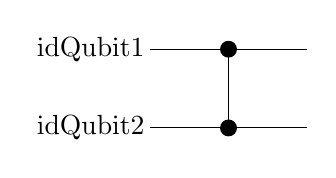
\begin{tikzpicture}[scale=.5] \node[draw=none] at (-3.5, 2) {idQubit1}; \node[draw=none] at (-3.5, 0) {idQubit2}; \draw (-2, 2) -- (2, 2); \draw[fill=black] (0, 2) circle (.2); \draw (0, 2) -- (0, 0); \draw (-2,0) -- (2, 0); \draw[fill=black] (0, 0) circle (.2); \end{tikzpicture} } \]


\begin{DoxyParams}[1]{Parameters}
\mbox{\tt in,out}  & {\em multi\+Qubit} & object representing the set of all qubits \\
\hline
\mbox{\tt in}  & {\em id\+Qubit1,id\+Qubit2} & qubits to operate upon \\
\hline
\end{DoxyParams}

\begin{DoxyExceptions}{Exceptions}
{\em exit\+With\+Error} & if {\ttfamily id\+Qubit1} or {\ttfamily id\+Qubit2} are outside \mbox{[}0, {\ttfamily multi\+Qubit.\+num\+Qubits}), or are equal \\
\hline
\end{DoxyExceptions}


Definition at line 1741 of file Qu\+E\+S\+T.\+c.



References Multi\+Qubit\+::chunk\+Id, extract\+Bit(), Complex\+Array\+::imag, Multi\+Qubit\+::num\+Amps, Multi\+Qubit\+::num\+Qubits, Qu\+E\+S\+T\+Assert(), Complex\+Array\+::real, R\+E\+AL, and Multi\+Qubit\+::state\+Vec.


\begin{DoxyCode}
1742 \{
1743     \textcolor{keywordtype}{long} \textcolor{keywordtype}{long} \textcolor{keywordtype}{int} index;
1744     \textcolor{keywordtype}{long} \textcolor{keywordtype}{long} \textcolor{keywordtype}{int} stateVecSize;
1745     \textcolor{keywordtype}{int} bit1, bit2;
1746 
1747     \textcolor{keyword}{const} \textcolor{keywordtype}{long} \textcolor{keywordtype}{long} \textcolor{keywordtype}{int} chunkSize=multiQubit.\mbox{\hyperlink{structMultiQubit_ae16f47d8b725c914fb7f66b6498d79db}{numAmps}};
1748     \textcolor{keyword}{const} \textcolor{keywordtype}{long} \textcolor{keywordtype}{long} \textcolor{keywordtype}{int} chunkId=multiQubit.\mbox{\hyperlink{structMultiQubit_ab10c88249fa3825d6227ceec01d37e37}{chunkId}};
1749 
1750     \mbox{\hyperlink{QuEST__env__local_8c_a3587b9d533e633ccf1abf9ad2ce45d8d}{QuESTAssert}}(idQubit1 >= 0 && idQubit1 < multiQubit.\mbox{\hyperlink{structMultiQubit_ab5b9795bdc6fb5855e1974dcbbaeb36f}{numQubits}}, 2, \_\_func\_\_);
1751     \mbox{\hyperlink{QuEST__env__local_8c_a3587b9d533e633ccf1abf9ad2ce45d8d}{QuESTAssert}}(idQubit2 >= 0 && idQubit2 < multiQubit.\mbox{\hyperlink{structMultiQubit_ab5b9795bdc6fb5855e1974dcbbaeb36f}{numQubits}}, 1, \_\_func\_\_);
1752     \mbox{\hyperlink{QuEST__env__local_8c_a3587b9d533e633ccf1abf9ad2ce45d8d}{QuESTAssert}}(idQubit1 != idQubit2, 3, \_\_func\_\_);
1753 
1754     \textcolor{comment}{// dimension of the state vector}
1755     stateVecSize = multiQubit.\mbox{\hyperlink{structMultiQubit_ae16f47d8b725c914fb7f66b6498d79db}{numAmps}};
1756     \mbox{\hyperlink{QuEST__precision_8h_a4b654506f18b8bfd61ad2a29a7e38c25}{REAL}} *stateVecReal = multiQubit.\mbox{\hyperlink{structMultiQubit_a45483190d6b01ef6b2f98f2bec9ab94f}{stateVec}}.\mbox{\hyperlink{structComplexArray_a4195cac6c784ea1b6271f1c7dba1548a}{real}};
1757     \mbox{\hyperlink{QuEST__precision_8h_a4b654506f18b8bfd61ad2a29a7e38c25}{REAL}} *stateVecImag = multiQubit.\mbox{\hyperlink{structMultiQubit_a45483190d6b01ef6b2f98f2bec9ab94f}{stateVec}}.\mbox{\hyperlink{structComplexArray_a79dde47c7ae530c79cebfdf57b225968}{imag}};
1758 
1759 \textcolor{preprocessor}{# ifdef \_OPENMP}
1760 \textcolor{preprocessor}{# pragma omp parallel for \(\backslash\)}
1761 \textcolor{preprocessor}{    default  (none)                          \(\backslash\)}
1762 \textcolor{preprocessor}{    shared   (stateVecSize, stateVecReal,stateVecImag ) \(\backslash\)}
1763 \textcolor{preprocessor}{    private  (index,bit1,bit2)                 \(\backslash\)}
1764 \textcolor{preprocessor}{    schedule (static)}
1765 \textcolor{preprocessor}{# endif}
1766     \textcolor{keywordflow}{for} (index=0; index<stateVecSize; index++) \{
1767         bit1 = \mbox{\hyperlink{QuEST_8c_a100463f6ec212c76a5fad99579000505}{extractBit}} (idQubit1, index+chunkId*chunkSize);
1768         bit2 = \mbox{\hyperlink{QuEST_8c_a100463f6ec212c76a5fad99579000505}{extractBit}} (idQubit2, index+chunkId*chunkSize);
1769         \textcolor{keywordflow}{if} (bit1 && bit2) \{
1770             stateVecReal [index] = - stateVecReal [index];
1771             stateVecImag [index] = - stateVecImag [index];
1772         \}
1773     \}
1774 \}
\end{DoxyCode}
\mbox{\Hypertarget{QuEST_8c_ad41f82b41149393a642391b67b3a287e}\label{QuEST_8c_ad41f82b41149393a642391b67b3a287e}} 
\index{Qu\+E\+S\+T.\+c@{Qu\+E\+S\+T.\+c}!controlled\+Rotate\+Around\+Axis@{controlled\+Rotate\+Around\+Axis}}
\index{controlled\+Rotate\+Around\+Axis@{controlled\+Rotate\+Around\+Axis}!Qu\+E\+S\+T.\+c@{Qu\+E\+S\+T.\+c}}
\paragraph{\texorpdfstring{controlled\+Rotate\+Around\+Axis()}{controlledRotateAroundAxis()}}
{\footnotesize\ttfamily void controlled\+Rotate\+Around\+Axis (\begin{DoxyParamCaption}\item[{\mbox{\hyperlink{structMultiQubit}{Multi\+Qubit}}}]{multi\+Qubit,  }\item[{const int}]{control\+Qubit,  }\item[{const int}]{target\+Qubit,  }\item[{\mbox{\hyperlink{QuEST__precision_8h_a4b654506f18b8bfd61ad2a29a7e38c25}{R\+E\+AL}}}]{angle,  }\item[{\mbox{\hyperlink{structVector}{Vector}}}]{axis }\end{DoxyParamCaption})}



Applies a controlled rotation by a given angle around a given vector on the Bloch-\/sphere. 

The vector must not be zero (else an error is thrown), but needn\textquotesingle{}t be unit magnitude.

For angle $\theta$ and axis vector $\vec{n}$, applies $R_{\hat{n}} = \exp \left(- i \frac{\theta}{2} \hat{n} \cdot \vec{\sigma} \right) $ to states where the target qubit is 1 ( $\vec{\sigma}$ is the vector of Pauli matrices).

\[ \setlength{\fboxrule}{0.01pt} \fbox{ 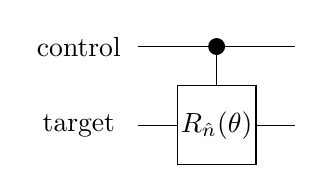
\begin{tikzpicture}[scale=.5] \node[draw=none] at (-3.5, 2) {control}; \node[draw=none] at (-3.5, 0) {target}; \draw (-2, 2) -- (2, 2); \draw[fill=black] (0, 2) circle (.2); \draw (0, 2) -- (0, 1); \draw (-2,0) -- (-1, 0); \draw (1, 0) -- (2, 0); \draw (-1,-1)--(-1,1)--(1,1)--(1,-1)--cycle; \node[draw=none] at (0, 0) {$R_{\hat{n}}(\theta)$}; \end{tikzpicture} } \]


\begin{DoxyParams}[1]{Parameters}
\mbox{\tt in,out}  & {\em multi\+Qubit} & object representing the set of all qubits \\
\hline
\mbox{\tt in}  & {\em control\+Qubit} & qubit with value 1 in the rotated states \\
\hline
\mbox{\tt in}  & {\em target\+Qubit} & qubit to rotate \\
\hline
\mbox{\tt in}  & {\em angle} & angle by which to rotate in radians \\
\hline
\mbox{\tt in}  & {\em axis} & vector around which to rotate (can be non-\/unit; will be normalised) \\
\hline
\end{DoxyParams}

\begin{DoxyExceptions}{Exceptions}
{\em exit\+With\+Error} & if either {\ttfamily control\+Qubit} or {\ttfamily target\+Qubit} are outside \mbox{[}0, {\ttfamily multi\+Qubit.\+num\+Qubits}) or are equal or if {\ttfamily axis} is the zero vector \\
\hline
\end{DoxyExceptions}


Definition at line 452 of file Qu\+E\+S\+T.\+c.



References controlled\+Compact\+Unitary(), Complex\+::imag, Complex\+::real, Vector\+::x, Vector\+::y, and Vector\+::z.



Referenced by controlled\+Rotate\+X(), controlled\+Rotate\+Y(), and controlled\+Rotate\+Z().


\begin{DoxyCode}
452                                                                                                            
                         \{
453 
454     \textcolor{keywordtype}{double} mag = sqrt(pow(axis.\mbox{\hyperlink{structVector_aac7abe171ba4bada50ed72acba6259fc}{x}},2) + pow(axis.\mbox{\hyperlink{structVector_a375ca805d4c808a53d7c4e0c737ae3de}{y}},2) + pow(axis.\mbox{\hyperlink{structVector_ad4e863651be7d6b7e2b28cd7445a0ccf}{z}},2));
455     \mbox{\hyperlink{structVector}{Vector}} unitAxis = \{axis.\mbox{\hyperlink{structVector_aac7abe171ba4bada50ed72acba6259fc}{x}}/mag, axis.\mbox{\hyperlink{structVector_a375ca805d4c808a53d7c4e0c737ae3de}{y}}/mag, axis.\mbox{\hyperlink{structVector_ad4e863651be7d6b7e2b28cd7445a0ccf}{z}}/mag\};
456 
457     \mbox{\hyperlink{structComplex}{Complex}} alpha, beta;
458     alpha.\mbox{\hyperlink{structComplex_a479ad939835457595fcca3ca55c06283}{real}} = cos(angle/2.0);
459     alpha.\mbox{\hyperlink{structComplex_a1151948284b21c0052f203f23ab931d9}{imag}} = -sin(angle/2.0)*unitAxis.\mbox{\hyperlink{structVector_ad4e863651be7d6b7e2b28cd7445a0ccf}{z}};       
460     beta.\mbox{\hyperlink{structComplex_a479ad939835457595fcca3ca55c06283}{real}} = sin(angle/2.0)*unitAxis.\mbox{\hyperlink{structVector_a375ca805d4c808a53d7c4e0c737ae3de}{y}};
461     beta.\mbox{\hyperlink{structComplex_a1151948284b21c0052f203f23ab931d9}{imag}} = -sin(angle/2.0)*unitAxis.\mbox{\hyperlink{structVector_aac7abe171ba4bada50ed72acba6259fc}{x}};
462     \mbox{\hyperlink{QuEST_8h_ab4812953bc457405b3aa05a4c2f64f4a}{controlledCompactUnitary}}(multiQubit, controlQubit, targetQubit, alpha, beta);
463 \}
\end{DoxyCode}
\mbox{\Hypertarget{QuEST_8c_ac6923ac57e67d9a21096e06f6a9012f6}\label{QuEST_8c_ac6923ac57e67d9a21096e06f6a9012f6}} 
\index{Qu\+E\+S\+T.\+c@{Qu\+E\+S\+T.\+c}!controlled\+RotateX@{controlled\+RotateX}}
\index{controlled\+RotateX@{controlled\+RotateX}!Qu\+E\+S\+T.\+c@{Qu\+E\+S\+T.\+c}}
\paragraph{\texorpdfstring{controlled\+Rotate\+X()}{controlledRotateX()}}
{\footnotesize\ttfamily void controlled\+RotateX (\begin{DoxyParamCaption}\item[{\mbox{\hyperlink{structMultiQubit}{Multi\+Qubit}}}]{multi\+Qubit,  }\item[{const int}]{control\+Qubit,  }\item[{const int}]{target\+Qubit,  }\item[{\mbox{\hyperlink{QuEST__precision_8h_a4b654506f18b8bfd61ad2a29a7e38c25}{R\+E\+AL}}}]{angle }\end{DoxyParamCaption})}



Applies a controlled rotation by a given angle around the X-\/axis of the Bloch-\/sphere. 

The target qubit is rotated in states where the control qubit has value 1.

\[ \setlength{\fboxrule}{0.01pt} \fbox{ 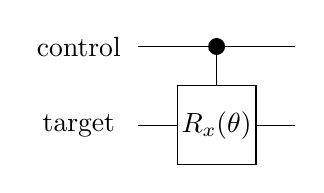
\begin{tikzpicture}[scale=.5] \node[draw=none] at (-3.5, 2) {control}; \node[draw=none] at (-3.5, 0) {target}; \draw (-2, 2) -- (2, 2); \draw[fill=black] (0, 2) circle (.2); \draw (0, 2) -- (0, 1); \draw (-2,0) -- (-1, 0); \draw (1, 0) -- (2, 0); \draw (-1,-1)--(-1,1)--(1,1)--(1,-1)--cycle; \node[draw=none] at (0, 0) {$R_x(\theta)$}; \end{tikzpicture} } \] ~\newline
 
\begin{DoxyParams}[1]{Parameters}
\mbox{\tt in,out}  & {\em multi\+Qubit} & object representing the set of all qubits \\
\hline
\mbox{\tt in}  & {\em control\+Qubit} & qubit which has value 1 in the rotated states \\
\hline
\mbox{\tt in}  & {\em tagret\+Qubit} & qubit to rotate \\
\hline
\mbox{\tt in}  & {\em angle} & angle by which to rotate the target qubit in radians \\
\hline
\end{DoxyParams}

\begin{DoxyExceptions}{Exceptions}
{\em exit\+With\+Error} & if either {\ttfamily control\+Qubit} or {\ttfamily target\+Qubit} are outside \mbox{[}0, {\ttfamily multi\+Qubit.\+num\+Qubits}) or are equal. \\
\hline
\end{DoxyExceptions}


Definition at line 465 of file Qu\+E\+S\+T.\+c.



References controlled\+Rotate\+Around\+Axis().


\begin{DoxyCode}
465                                                                                                         \{
466 
467     \mbox{\hyperlink{structVector}{Vector}} unitAxis = \{1, 0, 0\};
468     \mbox{\hyperlink{QuEST_8c_ad41f82b41149393a642391b67b3a287e}{controlledRotateAroundAxis}}(multiQubit, controlQubit, targetQubit, angle, 
      unitAxis);
469 \}
\end{DoxyCode}
\mbox{\Hypertarget{QuEST_8c_a71e90a2f7292116338c062934f9d1202}\label{QuEST_8c_a71e90a2f7292116338c062934f9d1202}} 
\index{Qu\+E\+S\+T.\+c@{Qu\+E\+S\+T.\+c}!controlled\+RotateY@{controlled\+RotateY}}
\index{controlled\+RotateY@{controlled\+RotateY}!Qu\+E\+S\+T.\+c@{Qu\+E\+S\+T.\+c}}
\paragraph{\texorpdfstring{controlled\+Rotate\+Y()}{controlledRotateY()}}
{\footnotesize\ttfamily void controlled\+RotateY (\begin{DoxyParamCaption}\item[{\mbox{\hyperlink{structMultiQubit}{Multi\+Qubit}}}]{multi\+Qubit,  }\item[{const int}]{control\+Qubit,  }\item[{const int}]{target\+Qubit,  }\item[{\mbox{\hyperlink{QuEST__precision_8h_a4b654506f18b8bfd61ad2a29a7e38c25}{R\+E\+AL}}}]{angle }\end{DoxyParamCaption})}



Applies a controlled rotation by a given angle around the Y-\/axis of the Bloch-\/sphere. 

The target qubit is rotated in states where the control qubit has value 1.

\[ \setlength{\fboxrule}{0.01pt} \fbox{ 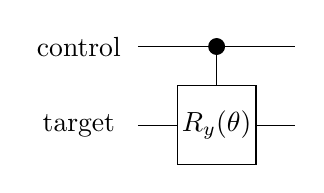
\begin{tikzpicture}[scale=.5] \node[draw=none] at (-3.5, 2) {control}; \node[draw=none] at (-3.5, 0) {target}; \draw (-2, 2) -- (2, 2); \draw[fill=black] (0, 2) circle (.2); \draw (0, 2) -- (0, 1); \draw (-2,0) -- (-1, 0); \draw (1, 0) -- (2, 0); \draw (-1,-1)--(-1,1)--(1,1)--(1,-1)--cycle; \node[draw=none] at (0, 0) {$R_y(\theta)$}; \end{tikzpicture} } \] ~\newline
 
\begin{DoxyParams}[1]{Parameters}
\mbox{\tt in,out}  & {\em multi\+Qubit} & object representing the set of all qubits \\
\hline
\mbox{\tt in}  & {\em control\+Qubit} & qubit which has value 1 in the rotated states \\
\hline
\mbox{\tt in}  & {\em tagret\+Qubit} & qubit to rotate \\
\hline
\mbox{\tt in}  & {\em angle} & angle by which to rotate the target qubit in radians \\
\hline
\end{DoxyParams}

\begin{DoxyExceptions}{Exceptions}
{\em exit\+With\+Error} & if either {\ttfamily control\+Qubit} or {\ttfamily target\+Qubit} are outside \mbox{[}0, {\ttfamily multi\+Qubit.\+num\+Qubits}) or are equal. \\
\hline
\end{DoxyExceptions}


Definition at line 471 of file Qu\+E\+S\+T.\+c.



References controlled\+Rotate\+Around\+Axis().


\begin{DoxyCode}
471                                                                                                         \{
472 
473     \mbox{\hyperlink{structVector}{Vector}} unitAxis = \{0, 1, 0\};
474     \mbox{\hyperlink{QuEST_8c_ad41f82b41149393a642391b67b3a287e}{controlledRotateAroundAxis}}(multiQubit, controlQubit, targetQubit, angle, 
      unitAxis);
475 \}
\end{DoxyCode}
\mbox{\Hypertarget{QuEST_8c_a668e5d2634b02e98bc73675ccb11d61c}\label{QuEST_8c_a668e5d2634b02e98bc73675ccb11d61c}} 
\index{Qu\+E\+S\+T.\+c@{Qu\+E\+S\+T.\+c}!controlled\+RotateZ@{controlled\+RotateZ}}
\index{controlled\+RotateZ@{controlled\+RotateZ}!Qu\+E\+S\+T.\+c@{Qu\+E\+S\+T.\+c}}
\paragraph{\texorpdfstring{controlled\+Rotate\+Z()}{controlledRotateZ()}}
{\footnotesize\ttfamily void controlled\+RotateZ (\begin{DoxyParamCaption}\item[{\mbox{\hyperlink{structMultiQubit}{Multi\+Qubit}}}]{multi\+Qubit,  }\item[{const int}]{control\+Qubit,  }\item[{const int}]{target\+Qubit,  }\item[{\mbox{\hyperlink{QuEST__precision_8h_a4b654506f18b8bfd61ad2a29a7e38c25}{R\+E\+AL}}}]{angle }\end{DoxyParamCaption})}



Applies a controlled rotation by a given angle around the Z-\/axis of the Bloch-\/sphere. 

The target qubit is rotated in states where the control qubit has value 1.

\[ \setlength{\fboxrule}{0.01pt} \fbox{ 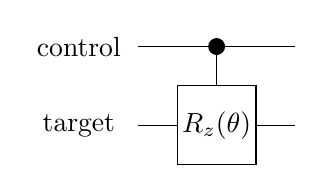
\begin{tikzpicture}[scale=.5] \node[draw=none] at (-3.5, 2) {control}; \node[draw=none] at (-3.5, 0) {target}; \draw (-2, 2) -- (2, 2); \draw[fill=black] (0, 2) circle (.2); \draw (0, 2) -- (0, 1); \draw (-2,0) -- (-1, 0); \draw (1, 0) -- (2, 0); \draw (-1,-1)--(-1,1)--(1,1)--(1,-1)--cycle; \node[draw=none] at (0, 0) {$R_z(\theta)$}; \end{tikzpicture} } \] ~\newline
 
\begin{DoxyParams}[1]{Parameters}
\mbox{\tt in,out}  & {\em multi\+Qubit} & object representing the set of all qubits \\
\hline
\mbox{\tt in}  & {\em control\+Qubit} & qubit which has value 1 in the rotated states \\
\hline
\mbox{\tt in}  & {\em tagret\+Qubit} & qubit to rotate \\
\hline
\mbox{\tt in}  & {\em angle} & angle by which to rotate the target qubit in radians \\
\hline
\end{DoxyParams}

\begin{DoxyExceptions}{Exceptions}
{\em exit\+With\+Error} & if either {\ttfamily control\+Qubit} or {\ttfamily target\+Qubit} are outside \mbox{[}0, {\ttfamily multi\+Qubit.\+num\+Qubits}) or are equal. \\
\hline
\end{DoxyExceptions}


Definition at line 477 of file Qu\+E\+S\+T.\+c.



References controlled\+Rotate\+Around\+Axis().


\begin{DoxyCode}
477                                                                                                         \{
478 
479     \mbox{\hyperlink{structVector}{Vector}} unitAxis = \{0, 0, 1\};
480     \mbox{\hyperlink{QuEST_8c_ad41f82b41149393a642391b67b3a287e}{controlledRotateAroundAxis}}(multiQubit, controlQubit, targetQubit, angle, 
      unitAxis);
481 \}
\end{DoxyCode}
\mbox{\Hypertarget{QuEST_8c_a642093063a1f889f61a1311f6d6f2d3f}\label{QuEST_8c_a642093063a1f889f61a1311f6d6f2d3f}} 
\index{Qu\+E\+S\+T.\+c@{Qu\+E\+S\+T.\+c}!controlled\+Unitary\+Distributed@{controlled\+Unitary\+Distributed}}
\index{controlled\+Unitary\+Distributed@{controlled\+Unitary\+Distributed}!Qu\+E\+S\+T.\+c@{Qu\+E\+S\+T.\+c}}
\paragraph{\texorpdfstring{controlled\+Unitary\+Distributed()}{controlledUnitaryDistributed()}}
{\footnotesize\ttfamily void controlled\+Unitary\+Distributed (\begin{DoxyParamCaption}\item[{\mbox{\hyperlink{structMultiQubit}{Multi\+Qubit}}}]{multi\+Qubit,  }\item[{const int}]{control\+Qubit,  }\item[{const int}]{target\+Qubit,  }\item[{\mbox{\hyperlink{structComplex}{Complex}}}]{rot1,  }\item[{\mbox{\hyperlink{structComplex}{Complex}}}]{rot2,  }\item[{\mbox{\hyperlink{structComplexArray}{Complex\+Array}}}]{state\+Vec\+Up,  }\item[{\mbox{\hyperlink{structComplexArray}{Complex\+Array}}}]{state\+Vec\+Lo,  }\item[{\mbox{\hyperlink{structComplexArray}{Complex\+Array}}}]{state\+Vec\+Out }\end{DoxyParamCaption})}



Rotate a single qubit in the state vector of probability amplitudes, given two complex numbers alpha and beta and a subset of the state vector with upper and lower block values stored seperately. 

Only perform the rotation where the control qubit is one.


\begin{DoxyParams}[1]{Parameters}
\mbox{\tt in,out}  & {\em multi\+Qubit} & object representing the set of qubits \\
\hline
\mbox{\tt in}  & {\em target\+Qubit} & qubit to rotate \\
\hline
\mbox{\tt in}  & {\em control\+Qubit} & qubit to determine whether or not to perform a rotation \\
\hline
\mbox{\tt in}  & {\em rot1} & rotation angle \\
\hline
\mbox{\tt in}  & {\em rot2} & rotation angle \\
\hline
\mbox{\tt in}  & {\em state\+Vec\+Up} & probability amplitudes in upper half of a block \\
\hline
\mbox{\tt in}  & {\em state\+Vec\+Lo} & probability amplitudes in lower half of a block \\
\hline
\mbox{\tt out}  & {\em state\+Vec\+Out} & array section to update (will correspond to either the lower or upper half of a block) \\
\hline
\end{DoxyParams}


Definition at line 985 of file Qu\+E\+S\+T.\+c.



References Multi\+Qubit\+::chunk\+Id, extract\+Bit(), Complex\+Array\+::imag, Complex\+::imag, Multi\+Qubit\+::num\+Amps, Complex\+Array\+::real, Complex\+::real, and R\+E\+AL.



Referenced by controlled\+Unitary().


\begin{DoxyCode}
990 \{
991 
992     \mbox{\hyperlink{QuEST__precision_8h_a4b654506f18b8bfd61ad2a29a7e38c25}{REAL}}   stateRealUp,stateRealLo,stateImagUp,stateImagLo;
993     \textcolor{keywordtype}{long} \textcolor{keywordtype}{long} \textcolor{keywordtype}{int} thisTask;  
994     \textcolor{keyword}{const} \textcolor{keywordtype}{long} \textcolor{keywordtype}{long} \textcolor{keywordtype}{int} numTasks=multiQubit.\mbox{\hyperlink{structMultiQubit_ae16f47d8b725c914fb7f66b6498d79db}{numAmps}};
995     \textcolor{keyword}{const} \textcolor{keywordtype}{long} \textcolor{keywordtype}{long} \textcolor{keywordtype}{int} chunkSize=multiQubit.\mbox{\hyperlink{structMultiQubit_ae16f47d8b725c914fb7f66b6498d79db}{numAmps}};
996     \textcolor{keyword}{const} \textcolor{keywordtype}{long} \textcolor{keywordtype}{long} \textcolor{keywordtype}{int} chunkId=multiQubit.\mbox{\hyperlink{structMultiQubit_ab10c88249fa3825d6227ceec01d37e37}{chunkId}};
997 
998     \textcolor{keywordtype}{int} controlBit;
999 
1000     \mbox{\hyperlink{QuEST__precision_8h_a4b654506f18b8bfd61ad2a29a7e38c25}{REAL}} rot1Real=rot1.\mbox{\hyperlink{structComplex_a479ad939835457595fcca3ca55c06283}{real}}, rot1Imag=rot1.\mbox{\hyperlink{structComplex_a1151948284b21c0052f203f23ab931d9}{imag}};
1001     \mbox{\hyperlink{QuEST__precision_8h_a4b654506f18b8bfd61ad2a29a7e38c25}{REAL}} rot2Real=rot2.\mbox{\hyperlink{structComplex_a479ad939835457595fcca3ca55c06283}{real}}, rot2Imag=rot2.\mbox{\hyperlink{structComplex_a1151948284b21c0052f203f23ab931d9}{imag}};
1002     \mbox{\hyperlink{QuEST__precision_8h_a4b654506f18b8bfd61ad2a29a7e38c25}{REAL}} *stateVecRealUp=stateVecUp.\mbox{\hyperlink{structComplexArray_a4195cac6c784ea1b6271f1c7dba1548a}{real}}, *stateVecImagUp=stateVecUp.
      \mbox{\hyperlink{structComplexArray_a79dde47c7ae530c79cebfdf57b225968}{imag}};
1003     \mbox{\hyperlink{QuEST__precision_8h_a4b654506f18b8bfd61ad2a29a7e38c25}{REAL}} *stateVecRealLo=stateVecLo.\mbox{\hyperlink{structComplexArray_a4195cac6c784ea1b6271f1c7dba1548a}{real}}, *stateVecImagLo=stateVecLo.
      \mbox{\hyperlink{structComplexArray_a79dde47c7ae530c79cebfdf57b225968}{imag}};
1004     \mbox{\hyperlink{QuEST__precision_8h_a4b654506f18b8bfd61ad2a29a7e38c25}{REAL}} *stateVecRealOut=stateVecOut.\mbox{\hyperlink{structComplexArray_a4195cac6c784ea1b6271f1c7dba1548a}{real}}, *stateVecImagOut=stateVecOut.
      \mbox{\hyperlink{structComplexArray_a79dde47c7ae530c79cebfdf57b225968}{imag}};
1005 
1006 \textcolor{preprocessor}{# ifdef \_OPENMP}
1007 \textcolor{preprocessor}{# pragma omp parallel \(\backslash\)}
1008 \textcolor{preprocessor}{    default  (none) \(\backslash\)}
1009 \textcolor{preprocessor}{    shared   (stateVecRealUp,stateVecImagUp,stateVecRealLo,stateVecImagLo,stateVecRealOut,stateVecImagOut, 
      \(\backslash\)}
1010 \textcolor{preprocessor}{            rot1Real,rot1Imag, rot2Real,rot2Imag) \(\backslash\)}
1011 \textcolor{preprocessor}{    private  (thisTask,stateRealUp,stateImagUp,stateRealLo,stateImagLo,controlBit)}
1012 \textcolor{preprocessor}{# endif}
1013     \{
1014 \textcolor{preprocessor}{# ifdef \_OPENMP}
1015 \textcolor{preprocessor}{# pragma omp for schedule (static)}
1016 \textcolor{preprocessor}{# endif}
1017         \textcolor{keywordflow}{for} (thisTask=0; thisTask<numTasks; thisTask++) \{
1018             controlBit = \mbox{\hyperlink{QuEST_8c_a100463f6ec212c76a5fad99579000505}{extractBit}} (controlQubit, thisTask+chunkId*chunkSize);
1019             \textcolor{keywordflow}{if} (controlBit)\{
1020                 \textcolor{comment}{// store current state vector values in temp variables}
1021                 stateRealUp = stateVecRealUp[thisTask];
1022                 stateImagUp = stateVecImagUp[thisTask];
1023 
1024                 stateRealLo = stateVecRealLo[thisTask];
1025                 stateImagLo = stateVecImagLo[thisTask];
1026 
1027                 stateVecRealOut[thisTask] = rot1Real*stateRealUp - rot1Imag*stateImagUp 
1028                     + rot2Real*stateRealLo - rot2Imag*stateImagLo;
1029                 stateVecImagOut[thisTask] = rot1Real*stateImagUp + rot1Imag*stateRealUp 
1030                     + rot2Real*stateImagLo + rot2Imag*stateRealLo;
1031             \}
1032         \}
1033     \}
1034 \}
\end{DoxyCode}
\mbox{\Hypertarget{QuEST_8c_a8a4afcff70195a306c082b8ed8d4e09a}\label{QuEST_8c_a8a4afcff70195a306c082b8ed8d4e09a}} 
\index{Qu\+E\+S\+T.\+c@{Qu\+E\+S\+T.\+c}!controlled\+Unitary\+Local@{controlled\+Unitary\+Local}}
\index{controlled\+Unitary\+Local@{controlled\+Unitary\+Local}!Qu\+E\+S\+T.\+c@{Qu\+E\+S\+T.\+c}}
\paragraph{\texorpdfstring{controlled\+Unitary\+Local()}{controlledUnitaryLocal()}}
{\footnotesize\ttfamily void controlled\+Unitary\+Local (\begin{DoxyParamCaption}\item[{\mbox{\hyperlink{structMultiQubit}{Multi\+Qubit}}}]{multi\+Qubit,  }\item[{const int}]{control\+Qubit,  }\item[{const int}]{target\+Qubit,  }\item[{\mbox{\hyperlink{structComplexMatrix2}{Complex\+Matrix2}}}]{u }\end{DoxyParamCaption})}



Definition at line 843 of file Qu\+E\+S\+T.\+c.



References Multi\+Qubit\+::chunk\+Id, extract\+Bit(), Complex\+Array\+::imag, Complex\+::imag, Multi\+Qubit\+::num\+Amps, Complex\+Matrix2\+::r0c0, Complex\+Matrix2\+::r0c1, Complex\+Matrix2\+::r1c0, Complex\+Matrix2\+::r1c1, Complex\+Array\+::real, Complex\+::real, R\+E\+AL, and Multi\+Qubit\+::state\+Vec.



Referenced by controlled\+Unitary().


\begin{DoxyCode}
845 \{
846     \textcolor{keywordtype}{long} \textcolor{keywordtype}{long} \textcolor{keywordtype}{int} sizeBlock, sizeHalfBlock;
847     \textcolor{keywordtype}{long} \textcolor{keywordtype}{long} \textcolor{keywordtype}{int} thisBlock, \textcolor{comment}{// current block}
848          indexUp,indexLo;    \textcolor{comment}{// current index and corresponding index in lower half block}
849 
850     \mbox{\hyperlink{QuEST__precision_8h_a4b654506f18b8bfd61ad2a29a7e38c25}{REAL}} stateRealUp,stateRealLo,stateImagUp,stateImagLo;
851     \textcolor{keywordtype}{long} \textcolor{keywordtype}{long} \textcolor{keywordtype}{int} thisTask;         
852     \textcolor{keyword}{const} \textcolor{keywordtype}{long} \textcolor{keywordtype}{long} \textcolor{keywordtype}{int} numTasks=multiQubit.\mbox{\hyperlink{structMultiQubit_ae16f47d8b725c914fb7f66b6498d79db}{numAmps}}>>1;
853     \textcolor{keyword}{const} \textcolor{keywordtype}{long} \textcolor{keywordtype}{long} \textcolor{keywordtype}{int} chunkSize=multiQubit.\mbox{\hyperlink{structMultiQubit_ae16f47d8b725c914fb7f66b6498d79db}{numAmps}};
854     \textcolor{keyword}{const} \textcolor{keywordtype}{long} \textcolor{keywordtype}{long} \textcolor{keywordtype}{int} chunkId=multiQubit.\mbox{\hyperlink{structMultiQubit_ab10c88249fa3825d6227ceec01d37e37}{chunkId}};
855 
856     \textcolor{keywordtype}{int} controlBit;
857 
858     \textcolor{comment}{// set dimensions}
859     sizeHalfBlock = 1LL << targetQubit;  
860     sizeBlock     = 2LL * sizeHalfBlock; 
861 
862     \textcolor{comment}{// Can't use multiQubit.stateVec as a private OMP var}
863     \mbox{\hyperlink{QuEST__precision_8h_a4b654506f18b8bfd61ad2a29a7e38c25}{REAL}} *stateVecReal = multiQubit.\mbox{\hyperlink{structMultiQubit_a45483190d6b01ef6b2f98f2bec9ab94f}{stateVec}}.\mbox{\hyperlink{structComplexArray_a4195cac6c784ea1b6271f1c7dba1548a}{real}};
864     \mbox{\hyperlink{QuEST__precision_8h_a4b654506f18b8bfd61ad2a29a7e38c25}{REAL}} *stateVecImag = multiQubit.\mbox{\hyperlink{structMultiQubit_a45483190d6b01ef6b2f98f2bec9ab94f}{stateVec}}.\mbox{\hyperlink{structComplexArray_a79dde47c7ae530c79cebfdf57b225968}{imag}};
865 
866 \textcolor{preprocessor}{# ifdef \_OPENMP}
867 \textcolor{preprocessor}{# pragma omp parallel \(\backslash\)}
868 \textcolor{preprocessor}{    default  (none) \(\backslash\)}
869 \textcolor{preprocessor}{    shared   (sizeBlock,sizeHalfBlock, stateVecReal,stateVecImag, u) \(\backslash\)}
870 \textcolor{preprocessor}{    private  (thisTask,thisBlock ,indexUp,indexLo,
       stateRealUp,stateImagUp,stateRealLo,stateImagLo,controlBit) }
871 \textcolor{preprocessor}{# endif}
872     \{
873 \textcolor{preprocessor}{# ifdef \_OPENMP}
874 \textcolor{preprocessor}{# pragma omp for schedule (static)}
875 \textcolor{preprocessor}{# endif}
876         \textcolor{keywordflow}{for} (thisTask=0; thisTask<numTasks; thisTask++) \{
877 
878             thisBlock   = thisTask / sizeHalfBlock;
879             indexUp     = thisBlock*sizeBlock + thisTask%sizeHalfBlock;
880             indexLo     = indexUp + sizeHalfBlock;
881 
882             controlBit = \mbox{\hyperlink{QuEST_8c_a100463f6ec212c76a5fad99579000505}{extractBit}} (controlQubit, indexUp+chunkId*chunkSize);
883             \textcolor{keywordflow}{if} (controlBit)\{
884                 \textcolor{comment}{// store current state vector values in temp variables}
885                 stateRealUp = stateVecReal[indexUp];
886                 stateImagUp = stateVecImag[indexUp];
887 
888                 stateRealLo = stateVecReal[indexLo];
889                 stateImagLo = stateVecImag[indexLo];
890 
891 
892                 \textcolor{comment}{// state[indexUp] = u00 * state[indexUp] + u01 * state[indexLo]}
893                 stateVecReal[indexUp] = u.\mbox{\hyperlink{structComplexMatrix2_ae72b4458233b077a636beee1892e81ff}{r0c0}}.\mbox{\hyperlink{structComplex_a479ad939835457595fcca3ca55c06283}{real}}*stateRealUp - u.\mbox{\hyperlink{structComplexMatrix2_ae72b4458233b077a636beee1892e81ff}{r0c0}}.
      \mbox{\hyperlink{structComplex_a1151948284b21c0052f203f23ab931d9}{imag}}*stateImagUp 
894                     + u.\mbox{\hyperlink{structComplexMatrix2_a0f3932f055a8b05cef361bce25d51172}{r0c1}}.\mbox{\hyperlink{structComplex_a479ad939835457595fcca3ca55c06283}{real}}*stateRealLo - u.\mbox{\hyperlink{structComplexMatrix2_a0f3932f055a8b05cef361bce25d51172}{r0c1}}.\mbox{\hyperlink{structComplex_a1151948284b21c0052f203f23ab931d9}{imag}}*stateImagLo;
895                 stateVecImag[indexUp] = u.\mbox{\hyperlink{structComplexMatrix2_ae72b4458233b077a636beee1892e81ff}{r0c0}}.\mbox{\hyperlink{structComplex_a479ad939835457595fcca3ca55c06283}{real}}*stateImagUp + u.\mbox{\hyperlink{structComplexMatrix2_ae72b4458233b077a636beee1892e81ff}{r0c0}}.
      \mbox{\hyperlink{structComplex_a1151948284b21c0052f203f23ab931d9}{imag}}*stateRealUp 
896                     + u.\mbox{\hyperlink{structComplexMatrix2_a0f3932f055a8b05cef361bce25d51172}{r0c1}}.\mbox{\hyperlink{structComplex_a479ad939835457595fcca3ca55c06283}{real}}*stateImagLo + u.\mbox{\hyperlink{structComplexMatrix2_a0f3932f055a8b05cef361bce25d51172}{r0c1}}.\mbox{\hyperlink{structComplex_a1151948284b21c0052f203f23ab931d9}{imag}}*stateRealLo;
897 
898                 \textcolor{comment}{// state[indexLo] = u10  * state[indexUp] + u11 * state[indexLo]}
899                 stateVecReal[indexLo] = u.\mbox{\hyperlink{structComplexMatrix2_ab98282015ed2065e53fbc9638e2583ab}{r1c0}}.\mbox{\hyperlink{structComplex_a479ad939835457595fcca3ca55c06283}{real}}*stateRealUp  - u.
      \mbox{\hyperlink{structComplexMatrix2_ab98282015ed2065e53fbc9638e2583ab}{r1c0}}.\mbox{\hyperlink{structComplex_a1151948284b21c0052f203f23ab931d9}{imag}}*stateImagUp 
900                     + u.\mbox{\hyperlink{structComplexMatrix2_a763007c3070802373549ba0350f83c8a}{r1c1}}.\mbox{\hyperlink{structComplex_a479ad939835457595fcca3ca55c06283}{real}}*stateRealLo  -  u.\mbox{\hyperlink{structComplexMatrix2_a763007c3070802373549ba0350f83c8a}{r1c1}}.\mbox{\hyperlink{structComplex_a1151948284b21c0052f203f23ab931d9}{imag}}*stateImagLo;
901                 stateVecImag[indexLo] = u.\mbox{\hyperlink{structComplexMatrix2_ab98282015ed2065e53fbc9638e2583ab}{r1c0}}.\mbox{\hyperlink{structComplex_a479ad939835457595fcca3ca55c06283}{real}}*stateImagUp + u.\mbox{\hyperlink{structComplexMatrix2_ab98282015ed2065e53fbc9638e2583ab}{r1c0}}.
      \mbox{\hyperlink{structComplex_a1151948284b21c0052f203f23ab931d9}{imag}}*stateRealUp 
902                     + u.\mbox{\hyperlink{structComplexMatrix2_a763007c3070802373549ba0350f83c8a}{r1c1}}.\mbox{\hyperlink{structComplex_a479ad939835457595fcca3ca55c06283}{real}}*stateImagLo + u.\mbox{\hyperlink{structComplexMatrix2_a763007c3070802373549ba0350f83c8a}{r1c1}}.\mbox{\hyperlink{structComplex_a1151948284b21c0052f203f23ab931d9}{imag}}*stateRealLo;
903             \}
904         \} 
905     \}
906 
907 \}
\end{DoxyCode}
\mbox{\Hypertarget{QuEST_8c_a9c02591bc64c2918503afa231d90d83f}\label{QuEST_8c_a9c02591bc64c2918503afa231d90d83f}} 
\index{Qu\+E\+S\+T.\+c@{Qu\+E\+S\+T.\+c}!create\+Multi\+Qubit@{create\+Multi\+Qubit}}
\index{create\+Multi\+Qubit@{create\+Multi\+Qubit}!Qu\+E\+S\+T.\+c@{Qu\+E\+S\+T.\+c}}
\paragraph{\texorpdfstring{create\+Multi\+Qubit()}{createMultiQubit()}}
{\footnotesize\ttfamily void create\+Multi\+Qubit (\begin{DoxyParamCaption}\item[{\mbox{\hyperlink{structMultiQubit}{Multi\+Qubit}} $\ast$}]{multi\+Qubit,  }\item[{int}]{num\+Qubits,  }\item[{\mbox{\hyperlink{structQuESTEnv}{Qu\+E\+S\+T\+Env}}}]{env }\end{DoxyParamCaption})}



Create a \mbox{\hyperlink{structMultiQubit}{Multi\+Qubit}} object representing a set of qubits. 

Allocate space for state vector of probability amplitudes, including space for temporary values to be copied from one other chunk if running the distributed version. Define properties related to the size of the set of qubits. init\+State\+Zero should be called after this to initialise the qubits to the zero state.


\begin{DoxyParams}[1]{Parameters}
\mbox{\tt in,out}  & {\em multi\+Qubit} & a pointer to an object representing the set of qubits \\
\hline
\mbox{\tt in}  & {\em num\+Qubits} & number of qubits in the system \\
\hline
\mbox{\tt in}  & {\em env} & object representing the execution environment (local, multinode etc) \\
\hline
\end{DoxyParams}

\begin{DoxyExceptions}{Exceptions}
{\em exit\+With\+Error} & if {\ttfamily num\+Qubits} $<$= 0 \\
\hline
\end{DoxyExceptions}


Definition at line 47 of file Qu\+E\+S\+T.\+c.



References Multi\+Qubit\+::chunk\+Id, Complex\+Array\+::imag, Multi\+Qubit\+::num\+Amps, Multi\+Qubit\+::num\+Chunks, Multi\+Qubit\+::num\+Qubits, Qu\+E\+S\+T\+Env\+::num\+Ranks, Multi\+Qubit\+::pair\+State\+Vec, Qu\+E\+S\+T\+Assert(), Qu\+E\+S\+T\+Env\+::rank, Complex\+Array\+::real, and Multi\+Qubit\+::state\+Vec.



Referenced by main().


\begin{DoxyCode}
48 \{
49     \mbox{\hyperlink{QuEST__env__local_8c_a3587b9d533e633ccf1abf9ad2ce45d8d}{QuESTAssert}}(numQubits>0, 9, \_\_func\_\_);
50     \textcolor{keywordtype}{long} \textcolor{keywordtype}{long} \textcolor{keywordtype}{int} numAmps = 1L << numQubits;
51     \textcolor{keywordtype}{long} \textcolor{keywordtype}{long} \textcolor{keywordtype}{int} numAmpsPerRank = numAmps/env.\mbox{\hyperlink{structQuESTEnv_af22aacd7c9905accae28484785c193b4}{numRanks}};
52 
53     multiQubit->\mbox{\hyperlink{structMultiQubit_a45483190d6b01ef6b2f98f2bec9ab94f}{stateVec}}.\mbox{\hyperlink{structComplexArray_a4195cac6c784ea1b6271f1c7dba1548a}{real}} = malloc(numAmpsPerRank * \textcolor{keyword}{sizeof}(*(multiQubit->
      \mbox{\hyperlink{structMultiQubit_a45483190d6b01ef6b2f98f2bec9ab94f}{stateVec}}.\mbox{\hyperlink{structComplexArray_a4195cac6c784ea1b6271f1c7dba1548a}{real}})));
54     multiQubit->\mbox{\hyperlink{structMultiQubit_a45483190d6b01ef6b2f98f2bec9ab94f}{stateVec}}.\mbox{\hyperlink{structComplexArray_a79dde47c7ae530c79cebfdf57b225968}{imag}} = malloc(numAmpsPerRank * \textcolor{keyword}{sizeof}(*(multiQubit->
      \mbox{\hyperlink{structMultiQubit_a45483190d6b01ef6b2f98f2bec9ab94f}{stateVec}}.\mbox{\hyperlink{structComplexArray_a79dde47c7ae530c79cebfdf57b225968}{imag}})));
55     \textcolor{keywordflow}{if} (env.\mbox{\hyperlink{structQuESTEnv_af22aacd7c9905accae28484785c193b4}{numRanks}}>1)\{
56         multiQubit->\mbox{\hyperlink{structMultiQubit_a76f7db4eab52d2b30f58f973ada809c5}{pairStateVec}}.\mbox{\hyperlink{structComplexArray_a4195cac6c784ea1b6271f1c7dba1548a}{real}} = malloc(numAmpsPerRank * \textcolor{keyword}{sizeof}(*(multiQubit->
      \mbox{\hyperlink{structMultiQubit_a76f7db4eab52d2b30f58f973ada809c5}{pairStateVec}}.\mbox{\hyperlink{structComplexArray_a4195cac6c784ea1b6271f1c7dba1548a}{real}})));
57         multiQubit->\mbox{\hyperlink{structMultiQubit_a76f7db4eab52d2b30f58f973ada809c5}{pairStateVec}}.\mbox{\hyperlink{structComplexArray_a79dde47c7ae530c79cebfdf57b225968}{imag}} = malloc(numAmpsPerRank * \textcolor{keyword}{sizeof}(*(multiQubit->
      \mbox{\hyperlink{structMultiQubit_a76f7db4eab52d2b30f58f973ada809c5}{pairStateVec}}.\mbox{\hyperlink{structComplexArray_a79dde47c7ae530c79cebfdf57b225968}{imag}})));
58     \}
59 
60     \textcolor{keywordflow}{if} ( (!(multiQubit->\mbox{\hyperlink{structMultiQubit_a45483190d6b01ef6b2f98f2bec9ab94f}{stateVec}}.\mbox{\hyperlink{structComplexArray_a4195cac6c784ea1b6271f1c7dba1548a}{real}}) || !(multiQubit->\mbox{\hyperlink{structMultiQubit_a45483190d6b01ef6b2f98f2bec9ab94f}{stateVec}}.
      \mbox{\hyperlink{structComplexArray_a79dde47c7ae530c79cebfdf57b225968}{imag}}))
61             && numAmpsPerRank ) \{
62         printf(\textcolor{stringliteral}{"Could not allocate memory!"});
63         exit (EXIT\_FAILURE);
64     \}
65 
66     \textcolor{keywordflow}{if} ( env.\mbox{\hyperlink{structQuESTEnv_af22aacd7c9905accae28484785c193b4}{numRanks}}>1 && (!(multiQubit->\mbox{\hyperlink{structMultiQubit_a76f7db4eab52d2b30f58f973ada809c5}{pairStateVec}}.\mbox{\hyperlink{structComplexArray_a4195cac6c784ea1b6271f1c7dba1548a}{real}}) || !(multiQubit->
      \mbox{\hyperlink{structMultiQubit_a76f7db4eab52d2b30f58f973ada809c5}{pairStateVec}}.\mbox{\hyperlink{structComplexArray_a79dde47c7ae530c79cebfdf57b225968}{imag}}))
67             && numAmpsPerRank ) \{
68         printf(\textcolor{stringliteral}{"Could not allocate memory!"});
69         exit (EXIT\_FAILURE);
70     \}
71 
72     multiQubit->\mbox{\hyperlink{structMultiQubit_ab5b9795bdc6fb5855e1974dcbbaeb36f}{numQubits}} = numQubits;
73     multiQubit->\mbox{\hyperlink{structMultiQubit_ae16f47d8b725c914fb7f66b6498d79db}{numAmps}} = numAmpsPerRank;
74     multiQubit->\mbox{\hyperlink{structMultiQubit_ab10c88249fa3825d6227ceec01d37e37}{chunkId}} = env.\mbox{\hyperlink{structQuESTEnv_aa648bb336cf8598467cb62db00b9cee8}{rank}};
75     multiQubit->\mbox{\hyperlink{structMultiQubit_acd43f2f57991709c9e94f73662c972b2}{numChunks}} = env.\mbox{\hyperlink{structQuESTEnv_af22aacd7c9905accae28484785c193b4}{numRanks}};
76 
77 \}
\end{DoxyCode}
\mbox{\Hypertarget{QuEST_8c_ae5d6acc322314d7a3d8a2eccf00d3b19}\label{QuEST_8c_ae5d6acc322314d7a3d8a2eccf00d3b19}} 
\index{Qu\+E\+S\+T.\+c@{Qu\+E\+S\+T.\+c}!destroy\+Multi\+Qubit@{destroy\+Multi\+Qubit}}
\index{destroy\+Multi\+Qubit@{destroy\+Multi\+Qubit}!Qu\+E\+S\+T.\+c@{Qu\+E\+S\+T.\+c}}
\paragraph{\texorpdfstring{destroy\+Multi\+Qubit()}{destroyMultiQubit()}}
{\footnotesize\ttfamily void destroy\+Multi\+Qubit (\begin{DoxyParamCaption}\item[{\mbox{\hyperlink{structMultiQubit}{Multi\+Qubit}}}]{multi\+Qubit,  }\item[{\mbox{\hyperlink{structQuESTEnv}{Qu\+E\+S\+T\+Env}}}]{env }\end{DoxyParamCaption})}



Deallocate a \mbox{\hyperlink{structMultiQubit}{Multi\+Qubit}} object representing a set of qubits. 

Free memory allocated to state vector of probability amplitudes, including temporary vector for values copied from another chunk if running the distributed version.


\begin{DoxyParams}[1]{Parameters}
\mbox{\tt in,out}  & {\em multi\+Qubit} & object to be deallocated \\
\hline
\mbox{\tt in}  & {\em env} & object representing the execution environment (local, multinode etc) \\
\hline
\end{DoxyParams}


Definition at line 79 of file Qu\+E\+S\+T.\+c.



References Complex\+Array\+::imag, Qu\+E\+S\+T\+Env\+::num\+Ranks, Multi\+Qubit\+::pair\+State\+Vec, Complex\+Array\+::real, and Multi\+Qubit\+::state\+Vec.



Referenced by main().


\begin{DoxyCode}
79                                                            \{
80     free(multiQubit.\mbox{\hyperlink{structMultiQubit_a45483190d6b01ef6b2f98f2bec9ab94f}{stateVec}}.\mbox{\hyperlink{structComplexArray_a4195cac6c784ea1b6271f1c7dba1548a}{real}});
81     free(multiQubit.\mbox{\hyperlink{structMultiQubit_a45483190d6b01ef6b2f98f2bec9ab94f}{stateVec}}.\mbox{\hyperlink{structComplexArray_a79dde47c7ae530c79cebfdf57b225968}{imag}});
82     \textcolor{keywordflow}{if} (env.\mbox{\hyperlink{structQuESTEnv_af22aacd7c9905accae28484785c193b4}{numRanks}}>1)\{
83         free(multiQubit.\mbox{\hyperlink{structMultiQubit_a76f7db4eab52d2b30f58f973ada809c5}{pairStateVec}}.\mbox{\hyperlink{structComplexArray_a4195cac6c784ea1b6271f1c7dba1548a}{real}});
84         free(multiQubit.\mbox{\hyperlink{structMultiQubit_a76f7db4eab52d2b30f58f973ada809c5}{pairStateVec}}.\mbox{\hyperlink{structComplexArray_a79dde47c7ae530c79cebfdf57b225968}{imag}});
85     \}
86 \}
\end{DoxyCode}
\mbox{\Hypertarget{QuEST_8c_a100463f6ec212c76a5fad99579000505}\label{QuEST_8c_a100463f6ec212c76a5fad99579000505}} 
\index{Qu\+E\+S\+T.\+c@{Qu\+E\+S\+T.\+c}!extract\+Bit@{extract\+Bit}}
\index{extract\+Bit@{extract\+Bit}!Qu\+E\+S\+T.\+c@{Qu\+E\+S\+T.\+c}}
\paragraph{\texorpdfstring{extract\+Bit()}{extractBit()}}
{\footnotesize\ttfamily static int extract\+Bit (\begin{DoxyParamCaption}\item[{const int}]{location\+Of\+Bit\+From\+Right,  }\item[{const long long int}]{the\+Encoded\+Number }\end{DoxyParamCaption})\hspace{0.3cm}{\ttfamily [static]}}



Get the value of the bit at a particular index in a number. 

S\+CB edit\+: new definition of extract\+Bit is much faster $\ast$$\ast$$\ast$ 
\begin{DoxyParams}[1]{Parameters}
\mbox{\tt in}  & {\em location\+Of\+Bit\+From\+Right} & location of bit in the\+Encoded\+Number \\
\hline
\mbox{\tt in}  & {\em the\+Encoded\+Number} & number to search \\
\hline
\end{DoxyParams}
\begin{DoxyReturn}{Returns}
the value of the bit in the\+Encoded\+Number 
\end{DoxyReturn}


Definition at line 1736 of file Qu\+E\+S\+T.\+c.



Referenced by controlled\+Compact\+Unitary\+Distributed(), controlled\+Compact\+Unitary\+Local(), controlled\+Not\+Distributed(), controlled\+Not\+Local(), controlled\+Phase\+Gate(), controlled\+Unitary\+Distributed(), controlled\+Unitary\+Local(), and init\+State\+Of\+Single\+Qubit().


\begin{DoxyCode}
1737 \{
1738     \textcolor{keywordflow}{return} (theEncodedNumber & ( 1LL << locationOfBitFromRight )) >> locationOfBitFromRight;
1739 \}
\end{DoxyCode}
\mbox{\Hypertarget{QuEST_8c_a9ac9bb717a889f09d307eda9f0b65957}\label{QuEST_8c_a9ac9bb717a889f09d307eda9f0b65957}} 
\index{Qu\+E\+S\+T.\+c@{Qu\+E\+S\+T.\+c}!find\+Probability\+Of\+Zero\+Distributed@{find\+Probability\+Of\+Zero\+Distributed}}
\index{find\+Probability\+Of\+Zero\+Distributed@{find\+Probability\+Of\+Zero\+Distributed}!Qu\+E\+S\+T.\+c@{Qu\+E\+S\+T.\+c}}
\paragraph{\texorpdfstring{find\+Probability\+Of\+Zero\+Distributed()}{findProbabilityOfZeroDistributed()}}
{\footnotesize\ttfamily \mbox{\hyperlink{QuEST__precision_8h_a4b654506f18b8bfd61ad2a29a7e38c25}{R\+E\+AL}} find\+Probability\+Of\+Zero\+Distributed (\begin{DoxyParamCaption}\item[{\mbox{\hyperlink{structMultiQubit}{Multi\+Qubit}}}]{multi\+Qubit,  }\item[{const int}]{measure\+Qubit }\end{DoxyParamCaption})}



Measure the probability of a specified qubit being in the zero state across all amplitudes held in this chunk. 

Size of regions to skip is a multiple of chunk\+Size.


\begin{DoxyParams}[1]{Parameters}
\mbox{\tt in}  & {\em multi\+Qubit} & object representing the set of qubits \\
\hline
\mbox{\tt in}  & {\em measure\+Qubit} & qubit to measure \\
\hline
\end{DoxyParams}
\begin{DoxyReturn}{Returns}
probability of qubit measure\+Qubit being zero 
\end{DoxyReturn}


Definition at line 1692 of file Qu\+E\+S\+T.\+c.



References Complex\+Array\+::imag, Multi\+Qubit\+::num\+Amps, Complex\+Array\+::real, R\+E\+AL, and Multi\+Qubit\+::state\+Vec.



Referenced by find\+Probability\+Of\+Outcome().


\begin{DoxyCode}
1694 \{
1695     \textcolor{comment}{// ----- measured probability}
1696     \mbox{\hyperlink{QuEST__precision_8h_a4b654506f18b8bfd61ad2a29a7e38c25}{REAL}}   totalProbability;                                  \textcolor{comment}{// probability (returned) value}
1697     \textcolor{comment}{// ----- temp variables}
1698     \textcolor{keywordtype}{long} \textcolor{keywordtype}{long} \textcolor{keywordtype}{int} thisTask;                                   \textcolor{comment}{// task based approach for expose loop with
       small granularity}
1699     \textcolor{keywordtype}{long} \textcolor{keywordtype}{long} \textcolor{keywordtype}{int} numTasks=multiQubit.\mbox{\hyperlink{structMultiQubit_ae16f47d8b725c914fb7f66b6498d79db}{numAmps}};
1700 
1701     \textcolor{comment}{// ---------------------------------------------------------------- //}
1702     \textcolor{comment}{//            find probability                                      //}
1703     \textcolor{comment}{// ---------------------------------------------------------------- //}
1704 
1705     \textcolor{comment}{// initialise returned value}
1706     totalProbability = 0.0;
1707 
1708     \mbox{\hyperlink{QuEST__precision_8h_a4b654506f18b8bfd61ad2a29a7e38c25}{REAL}} *stateVecReal = multiQubit.\mbox{\hyperlink{structMultiQubit_a45483190d6b01ef6b2f98f2bec9ab94f}{stateVec}}.\mbox{\hyperlink{structComplexArray_a4195cac6c784ea1b6271f1c7dba1548a}{real}};
1709     \mbox{\hyperlink{QuEST__precision_8h_a4b654506f18b8bfd61ad2a29a7e38c25}{REAL}} *stateVecImag = multiQubit.\mbox{\hyperlink{structMultiQubit_a45483190d6b01ef6b2f98f2bec9ab94f}{stateVec}}.\mbox{\hyperlink{structComplexArray_a79dde47c7ae530c79cebfdf57b225968}{imag}};
1710 
1711 \textcolor{preprocessor}{# ifdef \_OPENMP}
1712 \textcolor{preprocessor}{# pragma omp parallel \(\backslash\)}
1713 \textcolor{preprocessor}{    shared    (numTasks,stateVecReal,stateVecImag) \(\backslash\)}
1714 \textcolor{preprocessor}{    private   (thisTask) \(\backslash\)}
1715 \textcolor{preprocessor}{    reduction ( +:totalProbability )}
1716 \textcolor{preprocessor}{# endif}
1717     \{
1718 \textcolor{preprocessor}{# ifdef \_OPENMP}
1719 \textcolor{preprocessor}{# pragma omp for schedule  (static)}
1720 \textcolor{preprocessor}{# endif}
1721         \textcolor{keywordflow}{for} (thisTask=0; thisTask<numTasks; thisTask++) \{
1722             totalProbability += stateVecReal[thisTask]*stateVecReal[thisTask]
1723                 + stateVecImag[thisTask]*stateVecImag[thisTask];
1724         \}
1725     \}
1726 
1727     \textcolor{keywordflow}{return} totalProbability;
1728 \}
\end{DoxyCode}
\mbox{\Hypertarget{QuEST_8c_a7c02cd0e1b4eac19771a0525f023249e}\label{QuEST_8c_a7c02cd0e1b4eac19771a0525f023249e}} 
\index{Qu\+E\+S\+T.\+c@{Qu\+E\+S\+T.\+c}!find\+Probability\+Of\+Zero\+Local@{find\+Probability\+Of\+Zero\+Local}}
\index{find\+Probability\+Of\+Zero\+Local@{find\+Probability\+Of\+Zero\+Local}!Qu\+E\+S\+T.\+c@{Qu\+E\+S\+T.\+c}}
\paragraph{\texorpdfstring{find\+Probability\+Of\+Zero\+Local()}{findProbabilityOfZeroLocal()}}
{\footnotesize\ttfamily \mbox{\hyperlink{QuEST__precision_8h_a4b654506f18b8bfd61ad2a29a7e38c25}{R\+E\+AL}} find\+Probability\+Of\+Zero\+Local (\begin{DoxyParamCaption}\item[{\mbox{\hyperlink{structMultiQubit}{Multi\+Qubit}}}]{multi\+Qubit,  }\item[{const int}]{measure\+Qubit }\end{DoxyParamCaption})}



Measure the total probability of a specified qubit being in the zero state across all amplitudes in this chunk. 

Size of regions to skip is less than the size of one chunk. ~\newline
 
\begin{DoxyParams}[1]{Parameters}
\mbox{\tt in}  & {\em multi\+Qubit} & object representing the set of qubits \\
\hline
\mbox{\tt in}  & {\em measure\+Qubit} & qubit to measure \\
\hline
\end{DoxyParams}
\begin{DoxyReturn}{Returns}
probability of qubit measure\+Qubit being zero 
\end{DoxyReturn}


Definition at line 1636 of file Qu\+E\+S\+T.\+c.



References Complex\+Array\+::imag, Multi\+Qubit\+::num\+Amps, Complex\+Array\+::real, R\+E\+AL, and Multi\+Qubit\+::state\+Vec.



Referenced by find\+Probability\+Of\+Outcome().


\begin{DoxyCode}
1638 \{
1639     \textcolor{comment}{// ----- sizes}
1640     \textcolor{keywordtype}{long} \textcolor{keywordtype}{long} \textcolor{keywordtype}{int} sizeBlock,                                  \textcolor{comment}{// size of blocks}
1641          sizeHalfBlock;                                       \textcolor{comment}{// size of blocks halved}
1642     \textcolor{comment}{// ----- indices}
1643     \textcolor{keywordtype}{long} \textcolor{keywordtype}{long} \textcolor{keywordtype}{int} thisBlock,                                  \textcolor{comment}{// current block}
1644          index;                                               \textcolor{comment}{// current index for first half block}
1645     \textcolor{comment}{// ----- measured probability}
1646     \mbox{\hyperlink{QuEST__precision_8h_a4b654506f18b8bfd61ad2a29a7e38c25}{REAL}}   totalProbability;                                  \textcolor{comment}{// probability (returned) value}
1647     \textcolor{comment}{// ----- temp variables}
1648     \textcolor{keywordtype}{long} \textcolor{keywordtype}{long} \textcolor{keywordtype}{int} thisTask;                                   
1649     \textcolor{keywordtype}{long} \textcolor{keywordtype}{long} \textcolor{keywordtype}{int} numTasks=multiQubit.\mbox{\hyperlink{structMultiQubit_ae16f47d8b725c914fb7f66b6498d79db}{numAmps}}>>1;
1650 
1651     \textcolor{comment}{// ---------------------------------------------------------------- //}
1652     \textcolor{comment}{//            dimensions                                            //}
1653     \textcolor{comment}{// ---------------------------------------------------------------- //}
1654     sizeHalfBlock = 1LL << (measureQubit);                       \textcolor{comment}{// number of state vector elements to sum,}
1655     \textcolor{comment}{// and then the number to skip}
1656     sizeBlock     = 2LL * sizeHalfBlock;                         \textcolor{comment}{// size of blocks (pairs of measure and
       skip entries)}
1657 
1658     \textcolor{comment}{// initialise returned value}
1659     totalProbability = 0.0;
1660 
1661     \mbox{\hyperlink{QuEST__precision_8h_a4b654506f18b8bfd61ad2a29a7e38c25}{REAL}} *stateVecReal = multiQubit.\mbox{\hyperlink{structMultiQubit_a45483190d6b01ef6b2f98f2bec9ab94f}{stateVec}}.\mbox{\hyperlink{structComplexArray_a4195cac6c784ea1b6271f1c7dba1548a}{real}};
1662     \mbox{\hyperlink{QuEST__precision_8h_a4b654506f18b8bfd61ad2a29a7e38c25}{REAL}} *stateVecImag = multiQubit.\mbox{\hyperlink{structMultiQubit_a45483190d6b01ef6b2f98f2bec9ab94f}{stateVec}}.\mbox{\hyperlink{structComplexArray_a79dde47c7ae530c79cebfdf57b225968}{imag}};
1663 
1664 \textcolor{preprocessor}{# ifdef \_OPENMP}
1665 \textcolor{preprocessor}{# pragma omp parallel \(\backslash\)}
1666 \textcolor{preprocessor}{    shared    (numTasks,sizeBlock,sizeHalfBlock, stateVecReal,stateVecImag) \(\backslash\)}
1667 \textcolor{preprocessor}{    private   (thisTask,thisBlock,index) \(\backslash\)}
1668 \textcolor{preprocessor}{    reduction ( +:totalProbability )}
1669 \textcolor{preprocessor}{# endif }
1670     \{
1671 \textcolor{preprocessor}{# ifdef \_OPENMP}
1672 \textcolor{preprocessor}{# pragma omp for schedule  (static)}
1673 \textcolor{preprocessor}{# endif}
1674         \textcolor{keywordflow}{for} (thisTask=0; thisTask<numTasks; thisTask++) \{
1675             thisBlock = thisTask / sizeHalfBlock;
1676             index     = thisBlock*sizeBlock + thisTask%sizeHalfBlock;
1677 
1678             totalProbability += stateVecReal[index]*stateVecReal[index]
1679                 + stateVecImag[index]*stateVecImag[index];
1680         \}
1681     \}
1682     \textcolor{keywordflow}{return} totalProbability;
1683 \}
\end{DoxyCode}
\mbox{\Hypertarget{QuEST_8c_a8f10aabf9f607f19093aee54630caa21}\label{QuEST_8c_a8f10aabf9f607f19093aee54630caa21}} 
\index{Qu\+E\+S\+T.\+c@{Qu\+E\+S\+T.\+c}!get\+Environment\+String@{get\+Environment\+String}}
\index{get\+Environment\+String@{get\+Environment\+String}!Qu\+E\+S\+T.\+c@{Qu\+E\+S\+T.\+c}}
\paragraph{\texorpdfstring{get\+Environment\+String()}{getEnvironmentString()}}
{\footnotesize\ttfamily void get\+Environment\+String (\begin{DoxyParamCaption}\item[{\mbox{\hyperlink{structQuESTEnv}{Qu\+E\+S\+T\+Env}}}]{env,  }\item[{\mbox{\hyperlink{structMultiQubit}{Multi\+Qubit}}}]{multi\+Qubit,  }\item[{char}]{str\mbox{[}200\mbox{]} }\end{DoxyParamCaption})}



Definition at line 139 of file Qu\+E\+S\+T.\+c.



References Multi\+Qubit\+::num\+Qubits, and Qu\+E\+S\+T\+Env\+::num\+Ranks.


\begin{DoxyCode}
139                                                                              \{
140     \textcolor{keywordtype}{int} numThreads=1;
141 \textcolor{preprocessor}{# ifdef \_OPENMP}
142     numThreads=omp\_get\_max\_threads(); 
143 \textcolor{preprocessor}{# endif}
144     sprintf(str, \textcolor{stringliteral}{"%dqubits\_CPU\_%dranksx%dthreads"}, multiQubit.\mbox{\hyperlink{structMultiQubit_ab5b9795bdc6fb5855e1974dcbbaeb36f}{numQubits}}, env.
      \mbox{\hyperlink{structQuESTEnv_af22aacd7c9905accae28484785c193b4}{numRanks}}, numThreads);
145 \}
\end{DoxyCode}
\mbox{\Hypertarget{QuEST_8c_a799b10447d6dbdaf960a4d3eedd22014}\label{QuEST_8c_a799b10447d6dbdaf960a4d3eedd22014}} 
\index{Qu\+E\+S\+T.\+c@{Qu\+E\+S\+T.\+c}!get\+Prob\+El@{get\+Prob\+El}}
\index{get\+Prob\+El@{get\+Prob\+El}!Qu\+E\+S\+T.\+c@{Qu\+E\+S\+T.\+c}}
\paragraph{\texorpdfstring{get\+Prob\+El()}{getProbEl()}}
{\footnotesize\ttfamily \mbox{\hyperlink{QuEST__precision_8h_a4b654506f18b8bfd61ad2a29a7e38c25}{R\+E\+AL}} get\+Prob\+El (\begin{DoxyParamCaption}\item[{\mbox{\hyperlink{structMultiQubit}{Multi\+Qubit}}}]{multi\+Qubit,  }\item[{long long int}]{index }\end{DoxyParamCaption})}



Get the probability of the state at an index in the full state vector. 


\begin{DoxyParams}[1]{Parameters}
\mbox{\tt in}  & {\em multi\+Qubit} & object representing a set of qubits \\
\hline
\mbox{\tt in}  & {\em index} & index in state vector of probability amplitudes \\
\hline
\end{DoxyParams}
\begin{DoxyReturn}{Returns}
real\+El$\ast$real\+El + imag\+El$\ast$imag\+El 
\end{DoxyReturn}

\begin{DoxyExceptions}{Exceptions}
{\em exit\+With\+Error} & if {\ttfamily index} is outside \mbox{[}0, $2^{N}$) where $N = $ {\ttfamily multi\+Qubit.\+num\+Qubits} \\
\hline
\end{DoxyExceptions}


Definition at line 1979 of file Qu\+E\+S\+T.\+c.



References get\+Imag\+Amp\+El(), get\+Real\+Amp\+El(), and R\+E\+AL.



Referenced by main().


\begin{DoxyCode}
1979                                                           \{
1980     \mbox{\hyperlink{QuEST__precision_8h_a4b654506f18b8bfd61ad2a29a7e38c25}{REAL}} real;
1981     \mbox{\hyperlink{QuEST__precision_8h_a4b654506f18b8bfd61ad2a29a7e38c25}{REAL}} imag;
1982     real = \mbox{\hyperlink{QuEST_8h_a317b786f577fa6bc136ea7f0ee7330a7}{getRealAmpEl}}(multiQubit, index);
1983     imag = \mbox{\hyperlink{QuEST_8h_a3615f76fd5f57008d9b74bbd10533dd0}{getImagAmpEl}}(multiQubit, index);
1984     \textcolor{keywordflow}{return} real*real + imag*imag;
1985 \}
\end{DoxyCode}
\mbox{\Hypertarget{QuEST_8c_ae6a897066979fc52d977007d959ca09d}\label{QuEST_8c_ae6a897066979fc52d977007d959ca09d}} 
\index{Qu\+E\+S\+T.\+c@{Qu\+E\+S\+T.\+c}!hadamard\+Distributed@{hadamard\+Distributed}}
\index{hadamard\+Distributed@{hadamard\+Distributed}!Qu\+E\+S\+T.\+c@{Qu\+E\+S\+T.\+c}}
\paragraph{\texorpdfstring{hadamard\+Distributed()}{hadamardDistributed()}}
{\footnotesize\ttfamily void hadamard\+Distributed (\begin{DoxyParamCaption}\item[{\mbox{\hyperlink{structMultiQubit}{Multi\+Qubit}}}]{multi\+Qubit,  }\item[{const int}]{target\+Qubit,  }\item[{\mbox{\hyperlink{structComplexArray}{Complex\+Array}}}]{state\+Vec\+Up,  }\item[{\mbox{\hyperlink{structComplexArray}{Complex\+Array}}}]{state\+Vec\+Lo,  }\item[{\mbox{\hyperlink{structComplexArray}{Complex\+Array}}}]{state\+Vec\+Out,  }\item[{int}]{update\+Upper }\end{DoxyParamCaption})}



Rotate a single qubit by \{\{1,1\},\{1,-\/1\}\}/sqrt2. 

Operate on a subset of the state vector with upper and lower block values stored seperately. This rotation is just swapping upper and lower values, and state\+Vec\+In must already be the correct section for this chunk


\begin{DoxyParams}[1]{Parameters}
\mbox{\tt in,out}  & {\em multi\+Qubit} & object representing the set of qubits \\
\hline
\mbox{\tt in}  & {\em target\+Qubit} & qubit to rotate \\
\hline
\mbox{\tt in}  & {\em state\+Vec\+In} & probability amplitudes in lower or upper half of a block depending on chunk\+Id \\
\hline
\mbox{\tt in}  & {\em update\+Upper} & flag, 1\+: updating upper values, 0\+: updating lower values in block \\
\hline
\mbox{\tt out}  & {\em state\+Vec\+Out} & array section to update (will correspond to either the lower or upper half of a block) \\
\hline
\end{DoxyParams}


Definition at line 1439 of file Qu\+E\+S\+T.\+c.



References Complex\+Array\+::imag, Multi\+Qubit\+::num\+Amps, Complex\+Array\+::real, and R\+E\+AL.



Referenced by hadamard().


\begin{DoxyCode}
1444 \{
1445 
1446     \mbox{\hyperlink{QuEST__precision_8h_a4b654506f18b8bfd61ad2a29a7e38c25}{REAL}}   stateRealUp,stateRealLo,stateImagUp,stateImagLo;
1447     \textcolor{keywordtype}{long} \textcolor{keywordtype}{long} \textcolor{keywordtype}{int} thisTask;  
1448     \textcolor{keyword}{const} \textcolor{keywordtype}{long} \textcolor{keywordtype}{long} \textcolor{keywordtype}{int} numTasks=multiQubit.\mbox{\hyperlink{structMultiQubit_ae16f47d8b725c914fb7f66b6498d79db}{numAmps}};
1449 
1450     \textcolor{keywordtype}{int} sign;
1451     \textcolor{keywordflow}{if} (updateUpper) sign=1;
1452     \textcolor{keywordflow}{else} sign=-1;
1453 
1454     \mbox{\hyperlink{QuEST__precision_8h_a4b654506f18b8bfd61ad2a29a7e38c25}{REAL}} recRoot2 = 1.0/sqrt(2);
1455 
1456     \mbox{\hyperlink{QuEST__precision_8h_a4b654506f18b8bfd61ad2a29a7e38c25}{REAL}} *stateVecRealUp=stateVecUp.\mbox{\hyperlink{structComplexArray_a4195cac6c784ea1b6271f1c7dba1548a}{real}}, *stateVecImagUp=stateVecUp.
      \mbox{\hyperlink{structComplexArray_a79dde47c7ae530c79cebfdf57b225968}{imag}};
1457     \mbox{\hyperlink{QuEST__precision_8h_a4b654506f18b8bfd61ad2a29a7e38c25}{REAL}} *stateVecRealLo=stateVecLo.\mbox{\hyperlink{structComplexArray_a4195cac6c784ea1b6271f1c7dba1548a}{real}}, *stateVecImagLo=stateVecLo.
      \mbox{\hyperlink{structComplexArray_a79dde47c7ae530c79cebfdf57b225968}{imag}};
1458     \mbox{\hyperlink{QuEST__precision_8h_a4b654506f18b8bfd61ad2a29a7e38c25}{REAL}} *stateVecRealOut=stateVecOut.\mbox{\hyperlink{structComplexArray_a4195cac6c784ea1b6271f1c7dba1548a}{real}}, *stateVecImagOut=stateVecOut.
      \mbox{\hyperlink{structComplexArray_a79dde47c7ae530c79cebfdf57b225968}{imag}};
1459 
1460 \textcolor{preprocessor}{# ifdef \_OPENMP}
1461 \textcolor{preprocessor}{# pragma omp parallel \(\backslash\)}
1462 \textcolor{preprocessor}{    default  (none) \(\backslash\)}
1463 \textcolor{preprocessor}{    shared   (stateVecRealUp,stateVecImagUp,stateVecRealLo,stateVecImagLo,stateVecRealOut,stateVecImagOut, 
      \(\backslash\)}
1464 \textcolor{preprocessor}{            recRoot2, sign) \(\backslash\)}
1465 \textcolor{preprocessor}{    private  (thisTask,stateRealUp,stateImagUp,stateRealLo,stateImagLo)}
1466 \textcolor{preprocessor}{# endif}
1467     \{
1468 \textcolor{preprocessor}{# ifdef \_OPENMP}
1469 \textcolor{preprocessor}{# pragma omp for schedule (static)}
1470 \textcolor{preprocessor}{# endif}
1471         \textcolor{keywordflow}{for} (thisTask=0; thisTask<numTasks; thisTask++) \{
1472             \textcolor{comment}{// store current state vector values in temp variables}
1473             stateRealUp = stateVecRealUp[thisTask];
1474             stateImagUp = stateVecImagUp[thisTask];
1475 
1476             stateRealLo = stateVecRealLo[thisTask];
1477             stateImagLo = stateVecImagLo[thisTask];
1478 
1479             stateVecRealOut[thisTask] = recRoot2*(stateRealUp + sign*stateRealLo);
1480             stateVecImagOut[thisTask] = recRoot2*(stateImagUp + sign*stateImagLo);
1481         \}
1482     \}
1483 \}
\end{DoxyCode}
\mbox{\Hypertarget{QuEST_8c_aa9f0718b4dd794a3e1b143e3b153bfc5}\label{QuEST_8c_aa9f0718b4dd794a3e1b143e3b153bfc5}} 
\index{Qu\+E\+S\+T.\+c@{Qu\+E\+S\+T.\+c}!hadamard\+Local@{hadamard\+Local}}
\index{hadamard\+Local@{hadamard\+Local}!Qu\+E\+S\+T.\+c@{Qu\+E\+S\+T.\+c}}
\paragraph{\texorpdfstring{hadamard\+Local()}{hadamardLocal()}}
{\footnotesize\ttfamily void hadamard\+Local (\begin{DoxyParamCaption}\item[{\mbox{\hyperlink{structMultiQubit}{Multi\+Qubit}}}]{multi\+Qubit,  }\item[{const int}]{target\+Qubit }\end{DoxyParamCaption})}



Definition at line 1378 of file Qu\+E\+S\+T.\+c.



References Complex\+Array\+::imag, Multi\+Qubit\+::num\+Amps, Complex\+Array\+::real, R\+E\+AL, and Multi\+Qubit\+::state\+Vec.



Referenced by hadamard().


\begin{DoxyCode}
1379 \{
1380     \textcolor{keywordtype}{long} \textcolor{keywordtype}{long} \textcolor{keywordtype}{int} sizeBlock, sizeHalfBlock;
1381     \textcolor{keywordtype}{long} \textcolor{keywordtype}{long} \textcolor{keywordtype}{int} thisBlock, \textcolor{comment}{// current block}
1382          indexUp,indexLo;    \textcolor{comment}{// current index and corresponding index in lower half block}
1383 
1384     \mbox{\hyperlink{QuEST__precision_8h_a4b654506f18b8bfd61ad2a29a7e38c25}{REAL}} stateRealUp,stateRealLo,stateImagUp,stateImagLo;
1385     \textcolor{keywordtype}{long} \textcolor{keywordtype}{long} \textcolor{keywordtype}{int} thisTask;         
1386     \textcolor{keyword}{const} \textcolor{keywordtype}{long} \textcolor{keywordtype}{long} \textcolor{keywordtype}{int} numTasks=multiQubit.\mbox{\hyperlink{structMultiQubit_ae16f47d8b725c914fb7f66b6498d79db}{numAmps}}>>1;
1387 
1388     \textcolor{comment}{// set dimensions}
1389     sizeHalfBlock = 1LL << targetQubit;  
1390     sizeBlock     = 2LL * sizeHalfBlock; 
1391 
1392     \textcolor{comment}{// Can't use multiQubit.stateVec as a private OMP var}
1393     \mbox{\hyperlink{QuEST__precision_8h_a4b654506f18b8bfd61ad2a29a7e38c25}{REAL}} *stateVecReal = multiQubit.\mbox{\hyperlink{structMultiQubit_a45483190d6b01ef6b2f98f2bec9ab94f}{stateVec}}.\mbox{\hyperlink{structComplexArray_a4195cac6c784ea1b6271f1c7dba1548a}{real}};
1394     \mbox{\hyperlink{QuEST__precision_8h_a4b654506f18b8bfd61ad2a29a7e38c25}{REAL}} *stateVecImag = multiQubit.\mbox{\hyperlink{structMultiQubit_a45483190d6b01ef6b2f98f2bec9ab94f}{stateVec}}.\mbox{\hyperlink{structComplexArray_a79dde47c7ae530c79cebfdf57b225968}{imag}};
1395 
1396     \mbox{\hyperlink{QuEST__precision_8h_a4b654506f18b8bfd61ad2a29a7e38c25}{REAL}} recRoot2 = 1.0/sqrt(2);
1397 
1398 \textcolor{preprocessor}{# ifdef \_OPENMP}
1399 \textcolor{preprocessor}{# pragma omp parallel \(\backslash\)}
1400 \textcolor{preprocessor}{    default  (none) \(\backslash\)}
1401 \textcolor{preprocessor}{    shared   (sizeBlock,sizeHalfBlock, stateVecReal,stateVecImag, recRoot2) \(\backslash\)}
1402 \textcolor{preprocessor}{    private  (thisTask,thisBlock ,indexUp,indexLo, stateRealUp,stateImagUp,stateRealLo,stateImagLo) }
1403 \textcolor{preprocessor}{# endif}
1404     \{
1405 \textcolor{preprocessor}{# ifdef \_OPENMP}
1406 \textcolor{preprocessor}{# pragma omp for schedule (static)}
1407 \textcolor{preprocessor}{# endif}
1408         \textcolor{keywordflow}{for} (thisTask=0; thisTask<numTasks; thisTask++) \{
1409             thisBlock   = thisTask / sizeHalfBlock;
1410             indexUp     = thisBlock*sizeBlock + thisTask%sizeHalfBlock;
1411             indexLo     = indexUp + sizeHalfBlock;
1412 
1413             stateRealUp = stateVecReal[indexUp];
1414             stateImagUp = stateVecImag[indexUp];
1415 
1416             stateRealLo = stateVecReal[indexLo];
1417             stateImagLo = stateVecImag[indexLo];
1418 
1419             stateVecReal[indexUp] = recRoot2*(stateRealUp + stateRealLo);
1420             stateVecImag[indexUp] = recRoot2*(stateImagUp + stateImagLo);
1421 
1422             stateVecReal[indexLo] = recRoot2*(stateRealUp - stateRealLo);
1423             stateVecImag[indexLo] = recRoot2*(stateImagUp - stateImagLo);
1424         \} 
1425     \}
1426 \}
\end{DoxyCode}
\mbox{\Hypertarget{QuEST_8c_ab76254cfde16f0808476649507a1a2fc}\label{QuEST_8c_ab76254cfde16f0808476649507a1a2fc}} 
\index{Qu\+E\+S\+T.\+c@{Qu\+E\+S\+T.\+c}!hash\+String@{hash\+String}}
\index{hash\+String@{hash\+String}!Qu\+E\+S\+T.\+c@{Qu\+E\+S\+T.\+c}}
\paragraph{\texorpdfstring{hash\+String()}{hashString()}}
{\footnotesize\ttfamily unsigned long int hash\+String (\begin{DoxyParamCaption}\item[{char $\ast$}]{str }\end{DoxyParamCaption})}



Definition at line 2019 of file Qu\+E\+S\+T.\+c.



Referenced by Qu\+E\+S\+T\+Seed\+Random\+Default().


\begin{DoxyCode}
2019                                        \{
2020     \textcolor{keywordtype}{unsigned} \textcolor{keywordtype}{long} \textcolor{keywordtype}{int} hash = 5381;
2021     \textcolor{keywordtype}{int} c;
2022 
2023     \textcolor{keywordflow}{while} ((c = *str++))
2024         hash = ((hash << 5) + hash) + c; \textcolor{comment}{/* hash * 33 + c */}
2025 
2026     \textcolor{keywordflow}{return} hash;    
2027 \}
\end{DoxyCode}
\mbox{\Hypertarget{QuEST_8c_aea34d45aaea9e64ad3f7786bfb412d0c}\label{QuEST_8c_aea34d45aaea9e64ad3f7786bfb412d0c}} 
\index{Qu\+E\+S\+T.\+c@{Qu\+E\+S\+T.\+c}!init\+Classical\+State@{init\+Classical\+State}}
\index{init\+Classical\+State@{init\+Classical\+State}!Qu\+E\+S\+T.\+c@{Qu\+E\+S\+T.\+c}}
\paragraph{\texorpdfstring{init\+Classical\+State()}{initClassicalState()}}
{\footnotesize\ttfamily void init\+Classical\+State (\begin{DoxyParamCaption}\item[{\mbox{\hyperlink{structMultiQubit}{Multi\+Qubit}} $\ast$}]{multi\+Qubit,  }\item[{long long int}]{state\+Ind }\end{DoxyParamCaption})}



Initialise a set of $ N $ qubits to the classical state with index {\ttfamily state\+Ind}. 

Note $ | 00 \dots 00 \rangle $ has {\ttfamily state\+Ind} 0, $ | 00 \dots 01 \rangle $ has {\ttfamily state\+Ind} 1, $ | 11 \dots 11 \rangle $ has {\ttfamily state\+Ind} $ 2^N - 1 $, etc. Subsequent calls to get\+Prob\+El will yield 0 for all indices except {\ttfamily state\+Ind}.


\begin{DoxyParams}[1]{Parameters}
\mbox{\tt in,out}  & {\em multi\+Qubit} & a pointer to the object representing the set of qubits to be initialised \\
\hline
\mbox{\tt in}  & {\em state\+Ind} & the index (0 to the number of amplitudes, exclusive) of the state to give probability 1 \\
\hline
\end{DoxyParams}


Definition at line 216 of file Qu\+E\+S\+T.\+c.



References Multi\+Qubit\+::chunk\+Id, Complex\+Array\+::imag, Multi\+Qubit\+::num\+Amps, Complex\+Array\+::real, R\+E\+AL, and Multi\+Qubit\+::state\+Vec.


\begin{DoxyCode}
217 \{
218     \textcolor{keywordtype}{long} \textcolor{keywordtype}{long} \textcolor{keywordtype}{int} stateVecSize;
219     \textcolor{keywordtype}{long} \textcolor{keywordtype}{long} \textcolor{keywordtype}{int} index;
220 
221     \textcolor{comment}{// dimension of the state vector}
222     stateVecSize = multiQubit->\mbox{\hyperlink{structMultiQubit_ae16f47d8b725c914fb7f66b6498d79db}{numAmps}};
223 
224     \textcolor{comment}{// Can't use multiQubit->stateVec as a private OMP var}
225     \mbox{\hyperlink{QuEST__precision_8h_a4b654506f18b8bfd61ad2a29a7e38c25}{REAL}} *stateVecReal = multiQubit->\mbox{\hyperlink{structMultiQubit_a45483190d6b01ef6b2f98f2bec9ab94f}{stateVec}}.\mbox{\hyperlink{structComplexArray_a4195cac6c784ea1b6271f1c7dba1548a}{real}};
226     \mbox{\hyperlink{QuEST__precision_8h_a4b654506f18b8bfd61ad2a29a7e38c25}{REAL}} *stateVecImag = multiQubit->\mbox{\hyperlink{structMultiQubit_a45483190d6b01ef6b2f98f2bec9ab94f}{stateVec}}.\mbox{\hyperlink{structComplexArray_a79dde47c7ae530c79cebfdf57b225968}{imag}};
227 
228     \textcolor{comment}{// initialise the state to |0000..0000>}
229 \textcolor{preprocessor}{# ifdef \_OPENMP}
230 \textcolor{preprocessor}{# pragma omp parallel \(\backslash\)}
231 \textcolor{preprocessor}{    default  (none) \(\backslash\)}
232 \textcolor{preprocessor}{    shared   (stateInd, stateVecSize, stateVecReal, stateVecImag) \(\backslash\)}
233 \textcolor{preprocessor}{    private  (index) }
234 \textcolor{preprocessor}{# endif}
235     \{
236 \textcolor{preprocessor}{# ifdef \_OPENMP}
237 \textcolor{preprocessor}{# pragma omp for schedule (static)}
238 \textcolor{preprocessor}{# endif}
239         \textcolor{keywordflow}{for} (index=0; index<stateVecSize; index++) \{
240             stateVecReal[index] = 0.0;
241             stateVecImag[index] = 0.0;
242         \}
243     \}
244 
245         \textcolor{comment}{// give the specified classical state prob 1}
246     \textcolor{keywordflow}{if} (multiQubit->\mbox{\hyperlink{structMultiQubit_ab10c88249fa3825d6227ceec01d37e37}{chunkId}} == stateInd/stateVecSize)\{
247         stateVecReal[stateInd % stateVecSize] = 1.0;
248         stateVecImag[stateInd % stateVecSize] = 0.0;
249     \}
250 \}
\end{DoxyCode}
\mbox{\Hypertarget{QuEST_8c_a433876ee9f3bcc54af346300f571fc3c}\label{QuEST_8c_a433876ee9f3bcc54af346300f571fc3c}} 
\index{Qu\+E\+S\+T.\+c@{Qu\+E\+S\+T.\+c}!initialize\+State\+From\+Single\+File@{initialize\+State\+From\+Single\+File}}
\index{initialize\+State\+From\+Single\+File@{initialize\+State\+From\+Single\+File}!Qu\+E\+S\+T.\+c@{Qu\+E\+S\+T.\+c}}
\paragraph{\texorpdfstring{initialize\+State\+From\+Single\+File()}{initializeStateFromSingleFile()}}
{\footnotesize\ttfamily void initialize\+State\+From\+Single\+File (\begin{DoxyParamCaption}\item[{\mbox{\hyperlink{structMultiQubit}{Multi\+Qubit}} $\ast$}]{multi\+Qubit,  }\item[{char}]{filename\mbox{[}200\mbox{]},  }\item[{\mbox{\hyperlink{structQuESTEnv}{Qu\+E\+S\+T\+Env}}}]{env }\end{DoxyParamCaption})}

fix -- format needs to work for single precision values 

Definition at line 336 of file Qu\+E\+S\+T.\+c.



References Multi\+Qubit\+::chunk\+Id, Complex\+Array\+::imag, Multi\+Qubit\+::num\+Amps, Multi\+Qubit\+::num\+Chunks, Qu\+E\+S\+T\+Assert(), Complex\+Array\+::real, R\+E\+AL, Multi\+Qubit\+::state\+Vec, and sync\+Qu\+E\+S\+T\+Env().


\begin{DoxyCode}
336                                                                                             \{
337     \textcolor{keywordtype}{long} \textcolor{keywordtype}{long} \textcolor{keywordtype}{int} chunkSize, stateVecSize;
338     \textcolor{keywordtype}{long} \textcolor{keywordtype}{long} \textcolor{keywordtype}{int} indexInChunk, totalIndex;
339 
340     chunkSize = multiQubit->\mbox{\hyperlink{structMultiQubit_ae16f47d8b725c914fb7f66b6498d79db}{numAmps}};
341     stateVecSize = chunkSize*multiQubit->\mbox{\hyperlink{structMultiQubit_acd43f2f57991709c9e94f73662c972b2}{numChunks}};
342 
343     \mbox{\hyperlink{QuEST__precision_8h_a4b654506f18b8bfd61ad2a29a7e38c25}{REAL}} *stateVecReal = multiQubit->\mbox{\hyperlink{structMultiQubit_a45483190d6b01ef6b2f98f2bec9ab94f}{stateVec}}.\mbox{\hyperlink{structComplexArray_a4195cac6c784ea1b6271f1c7dba1548a}{real}};
344     \mbox{\hyperlink{QuEST__precision_8h_a4b654506f18b8bfd61ad2a29a7e38c25}{REAL}} *stateVecImag = multiQubit->\mbox{\hyperlink{structMultiQubit_a45483190d6b01ef6b2f98f2bec9ab94f}{stateVec}}.\mbox{\hyperlink{structComplexArray_a79dde47c7ae530c79cebfdf57b225968}{imag}};
345 
346     FILE *fp;
347     \textcolor{keywordtype}{char} line[200];
348 
349     \textcolor{keywordflow}{for} (\textcolor{keywordtype}{int} rank=0; rank<(multiQubit->\mbox{\hyperlink{structMultiQubit_acd43f2f57991709c9e94f73662c972b2}{numChunks}}); rank++)\{
350         \textcolor{keywordflow}{if} (rank==multiQubit->\mbox{\hyperlink{structMultiQubit_ab10c88249fa3825d6227ceec01d37e37}{chunkId}})\{
351             fp = fopen(filename, \textcolor{stringliteral}{"r"});
352             \mbox{\hyperlink{QuEST__env__local_8c_a3587b9d533e633ccf1abf9ad2ce45d8d}{QuESTAssert}}(fp!=NULL, 11, \_\_func\_\_);
353             indexInChunk = 0; totalIndex = 0;
354             \textcolor{keywordflow}{while} (fgets(line, \textcolor{keyword}{sizeof}(\textcolor{keywordtype}{char})*200, fp) != NULL && totalIndex<stateVecSize)\{
355                 \textcolor{keywordflow}{if} (line[0]!=\textcolor{charliteral}{'#'})\{
356                     \textcolor{keywordtype}{int} chunkId = totalIndex/chunkSize;
357                     \textcolor{keywordflow}{if} (chunkId==multiQubit->\mbox{\hyperlink{structMultiQubit_ab10c88249fa3825d6227ceec01d37e37}{chunkId}})\{
359                         sscanf(line, \textcolor{stringliteral}{"%lf, %lf"}, &(stateVecReal[indexInChunk]), 
360                                 &(stateVecImag[indexInChunk]));
361                         indexInChunk += 1;
362                     \}
363                     totalIndex += 1;
364                 \}
365             \}   
366             fclose(fp);
367         \}
368         \mbox{\hyperlink{QuEST_8h_a8d31fe2d1ad4d01e2a1f5f6b8bc15b77}{syncQuESTEnv}}(env);
369     \}
370 \}
\end{DoxyCode}
\mbox{\Hypertarget{QuEST_8c_a03b3577a891731d505bc4b879fcca9d3}\label{QuEST_8c_a03b3577a891731d505bc4b879fcca9d3}} 
\index{Qu\+E\+S\+T.\+c@{Qu\+E\+S\+T.\+c}!init\+State\+Debug@{init\+State\+Debug}}
\index{init\+State\+Debug@{init\+State\+Debug}!Qu\+E\+S\+T.\+c@{Qu\+E\+S\+T.\+c}}
\paragraph{\texorpdfstring{init\+State\+Debug()}{initStateDebug()}}
{\footnotesize\ttfamily void init\+State\+Debug (\begin{DoxyParamCaption}\item[{\mbox{\hyperlink{structMultiQubit}{Multi\+Qubit}} $\ast$}]{multi\+Qubit }\end{DoxyParamCaption})}



Initialise the state vector of probability amplitudes to an (unphysical) state with each component of each probability amplitude a unique floating point value. 

For debugging processes 
\begin{DoxyParams}[1]{Parameters}
\mbox{\tt in,out}  & {\em multi\+Qubit} & object representing the set of qubits to be initialised \\
\hline
\end{DoxyParams}


Definition at line 304 of file Qu\+E\+S\+T.\+c.



References Multi\+Qubit\+::chunk\+Id, Complex\+Array\+::imag, Multi\+Qubit\+::num\+Amps, Complex\+Array\+::real, R\+E\+AL, and Multi\+Qubit\+::state\+Vec.


\begin{DoxyCode}
305 \{
306     \textcolor{keywordtype}{long} \textcolor{keywordtype}{long} \textcolor{keywordtype}{int} chunkSize;
307     \textcolor{keywordtype}{long} \textcolor{keywordtype}{long} \textcolor{keywordtype}{int} index;
308 
309     \textcolor{comment}{// dimension of the state vector}
310     chunkSize = multiQubit->\mbox{\hyperlink{structMultiQubit_ae16f47d8b725c914fb7f66b6498d79db}{numAmps}};
311 
312     \textcolor{comment}{// Can't use multiQubit->stateVec as a private OMP var}
313     \mbox{\hyperlink{QuEST__precision_8h_a4b654506f18b8bfd61ad2a29a7e38c25}{REAL}} *stateVecReal = multiQubit->\mbox{\hyperlink{structMultiQubit_a45483190d6b01ef6b2f98f2bec9ab94f}{stateVec}}.\mbox{\hyperlink{structComplexArray_a4195cac6c784ea1b6271f1c7dba1548a}{real}};
314     \mbox{\hyperlink{QuEST__precision_8h_a4b654506f18b8bfd61ad2a29a7e38c25}{REAL}} *stateVecImag = multiQubit->\mbox{\hyperlink{structMultiQubit_a45483190d6b01ef6b2f98f2bec9ab94f}{stateVec}}.\mbox{\hyperlink{structComplexArray_a79dde47c7ae530c79cebfdf57b225968}{imag}};
315 
316     \mbox{\hyperlink{QuEST__precision_8h_a4b654506f18b8bfd61ad2a29a7e38c25}{REAL}} chunkOffset = (2.0*chunkSize*multiQubit->\mbox{\hyperlink{structMultiQubit_ab10c88249fa3825d6227ceec01d37e37}{chunkId}})/10.0;
317 
318     \textcolor{comment}{// initialise the state to |0000..0000>}
319 \textcolor{preprocessor}{# ifdef \_OPENMP}
320 \textcolor{preprocessor}{# pragma omp parallel \(\backslash\)}
321 \textcolor{preprocessor}{    default  (none) \(\backslash\)}
322 \textcolor{preprocessor}{    shared   (chunkSize, stateVecReal, stateVecImag, chunkOffset) \(\backslash\)}
323 \textcolor{preprocessor}{    private  (index) }
324 \textcolor{preprocessor}{# endif}
325     \{
326 \textcolor{preprocessor}{# ifdef \_OPENMP}
327 \textcolor{preprocessor}{# pragma omp for schedule (static)}
328 \textcolor{preprocessor}{# endif}
329         \textcolor{keywordflow}{for} (index=0; index<chunkSize; index++) \{
330             stateVecReal[index] = chunkOffset + (index*2.0)/10.0;
331             stateVecImag[index] = chunkOffset + (index*2.0+1.0)/10.0;
332         \}
333     \}
334 \}
\end{DoxyCode}
\mbox{\Hypertarget{QuEST_8c_a7169fd0442cbc3418f3fac4d13363ca2}\label{QuEST_8c_a7169fd0442cbc3418f3fac4d13363ca2}} 
\index{Qu\+E\+S\+T.\+c@{Qu\+E\+S\+T.\+c}!init\+State\+Of\+Single\+Qubit@{init\+State\+Of\+Single\+Qubit}}
\index{init\+State\+Of\+Single\+Qubit@{init\+State\+Of\+Single\+Qubit}!Qu\+E\+S\+T.\+c@{Qu\+E\+S\+T.\+c}}
\paragraph{\texorpdfstring{init\+State\+Of\+Single\+Qubit()}{initStateOfSingleQubit()}}
{\footnotesize\ttfamily void init\+State\+Of\+Single\+Qubit (\begin{DoxyParamCaption}\item[{\mbox{\hyperlink{structMultiQubit}{Multi\+Qubit}} $\ast$}]{multi\+Qubit,  }\item[{int}]{qubit\+Id,  }\item[{int}]{outcome }\end{DoxyParamCaption})}



Initialise the state vector of probability amplitudes such that one qubit is set to \textquotesingle{}outcome\textquotesingle{} and all other qubits are in an equal superposition of zero and one. 


\begin{DoxyParams}[1]{Parameters}
\mbox{\tt in,out}  & {\em multi\+Qubit} & object representing the set of qubits to be initialised \\
\hline
\mbox{\tt in}  & {\em qubit\+Id} & id of qubit to set to state \textquotesingle{}outcome\textquotesingle{} \\
\hline
\mbox{\tt in}  & {\em value} & of qubit \textquotesingle{}qubit\+Id\textquotesingle{} \\
\hline
\end{DoxyParams}


Definition at line 258 of file Qu\+E\+S\+T.\+c.



References Multi\+Qubit\+::chunk\+Id, extract\+Bit(), Complex\+Array\+::imag, Multi\+Qubit\+::num\+Amps, Multi\+Qubit\+::num\+Chunks, Complex\+Array\+::real, R\+E\+AL, and Multi\+Qubit\+::state\+Vec.


\begin{DoxyCode}
259 \{
260     \textcolor{keywordtype}{long} \textcolor{keywordtype}{long} \textcolor{keywordtype}{int} chunkSize, stateVecSize;
261     \textcolor{keywordtype}{long} \textcolor{keywordtype}{long} \textcolor{keywordtype}{int} index;
262     \textcolor{keywordtype}{int} bit;
263     \textcolor{keyword}{const} \textcolor{keywordtype}{long} \textcolor{keywordtype}{long} \textcolor{keywordtype}{int} chunkId=multiQubit->\mbox{\hyperlink{structMultiQubit_ab10c88249fa3825d6227ceec01d37e37}{chunkId}};
264 
265     \textcolor{comment}{// dimension of the state vector}
266     chunkSize = multiQubit->\mbox{\hyperlink{structMultiQubit_ae16f47d8b725c914fb7f66b6498d79db}{numAmps}};
267     stateVecSize = chunkSize*multiQubit->\mbox{\hyperlink{structMultiQubit_acd43f2f57991709c9e94f73662c972b2}{numChunks}};
268     \mbox{\hyperlink{QuEST__precision_8h_a4b654506f18b8bfd61ad2a29a7e38c25}{REAL}} normFactor = 1.0/sqrt((\mbox{\hyperlink{QuEST__precision_8h_a4b654506f18b8bfd61ad2a29a7e38c25}{REAL}})stateVecSize/2.0);
269 
270     \textcolor{comment}{// Can't use multiQubit->stateVec as a private OMP var}
271     \mbox{\hyperlink{QuEST__precision_8h_a4b654506f18b8bfd61ad2a29a7e38c25}{REAL}} *stateVecReal = multiQubit->\mbox{\hyperlink{structMultiQubit_a45483190d6b01ef6b2f98f2bec9ab94f}{stateVec}}.\mbox{\hyperlink{structComplexArray_a4195cac6c784ea1b6271f1c7dba1548a}{real}};
272     \mbox{\hyperlink{QuEST__precision_8h_a4b654506f18b8bfd61ad2a29a7e38c25}{REAL}} *stateVecImag = multiQubit->\mbox{\hyperlink{structMultiQubit_a45483190d6b01ef6b2f98f2bec9ab94f}{stateVec}}.\mbox{\hyperlink{structComplexArray_a79dde47c7ae530c79cebfdf57b225968}{imag}};
273 
274     \textcolor{comment}{// initialise the state to |0000..0000>}
275 \textcolor{preprocessor}{# ifdef \_OPENMP}
276 \textcolor{preprocessor}{# pragma omp parallel \(\backslash\)}
277 \textcolor{preprocessor}{    default  (none) \(\backslash\)}
278 \textcolor{preprocessor}{    shared   (chunkSize, stateVecReal, stateVecImag, normFactor, qubitId, outcome) \(\backslash\)}
279 \textcolor{preprocessor}{    private  (index, bit) }
280 \textcolor{preprocessor}{# endif}
281     \{
282 \textcolor{preprocessor}{# ifdef \_OPENMP}
283 \textcolor{preprocessor}{# pragma omp for schedule (static)}
284 \textcolor{preprocessor}{# endif}
285         \textcolor{keywordflow}{for} (index=0; index<chunkSize; index++) \{
286             bit = \mbox{\hyperlink{QuEST_8c_a100463f6ec212c76a5fad99579000505}{extractBit}}(qubitId, index+chunkId*chunkSize);
287             \textcolor{keywordflow}{if} (bit==outcome) \{
288                 stateVecReal[index] = normFactor;
289                 stateVecImag[index] = 0.0;
290             \} \textcolor{keywordflow}{else} \{
291                 stateVecReal[index] = 0.0;
292                 stateVecImag[index] = 0.0;
293             \}
294         \}
295     \}
296 \}
\end{DoxyCode}
\mbox{\Hypertarget{QuEST_8c_a43bcb279fc9717fbd06a19cdef48b9d8}\label{QuEST_8c_a43bcb279fc9717fbd06a19cdef48b9d8}} 
\index{Qu\+E\+S\+T.\+c@{Qu\+E\+S\+T.\+c}!init\+State\+Plus@{init\+State\+Plus}}
\index{init\+State\+Plus@{init\+State\+Plus}!Qu\+E\+S\+T.\+c@{Qu\+E\+S\+T.\+c}}
\paragraph{\texorpdfstring{init\+State\+Plus()}{initStatePlus()}}
{\footnotesize\ttfamily void init\+State\+Plus (\begin{DoxyParamCaption}\item[{\mbox{\hyperlink{structMultiQubit}{Multi\+Qubit}} $\ast$}]{multi\+Qubit }\end{DoxyParamCaption})}



Initialise a set of $ N $ qubits to the plus state $ {| + \rangle}^{\otimes N} = \frac{1}{\sqrt{2^N}} (| 0 \rangle + | 1 \rangle)^{\otimes N} $. 

This is the product state of $N$ qubits where every classical state is uniformly populated with real coefficient $\frac{1}{\sqrt{2^N}}$. This is equivalent to applying a Hadamard to every qubit in the zero state\+: $ \hat{H}^{\otimes N} {|0\rangle}^{\otimes N} $


\begin{DoxyParams}[1]{Parameters}
\mbox{\tt in,out}  & {\em multi\+Qubit} & a pointer to the object representing the set of qubits to be initialised \\
\hline
\end{DoxyParams}


Definition at line 183 of file Qu\+E\+S\+T.\+c.



References Complex\+Array\+::imag, Multi\+Qubit\+::num\+Amps, Multi\+Qubit\+::num\+Chunks, Complex\+Array\+::real, R\+E\+AL, and Multi\+Qubit\+::state\+Vec.


\begin{DoxyCode}
184 \{
185     \textcolor{keywordtype}{long} \textcolor{keywordtype}{long} \textcolor{keywordtype}{int} chunkSize, stateVecSize;
186     \textcolor{keywordtype}{long} \textcolor{keywordtype}{long} \textcolor{keywordtype}{int} index;
187 
188     \textcolor{comment}{// dimension of the state vector}
189     chunkSize = multiQubit->\mbox{\hyperlink{structMultiQubit_ae16f47d8b725c914fb7f66b6498d79db}{numAmps}};
190     stateVecSize = chunkSize*multiQubit->\mbox{\hyperlink{structMultiQubit_acd43f2f57991709c9e94f73662c972b2}{numChunks}};
191     \mbox{\hyperlink{QuEST__precision_8h_a4b654506f18b8bfd61ad2a29a7e38c25}{REAL}} normFactor = 1.0/sqrt((\mbox{\hyperlink{QuEST__precision_8h_a4b654506f18b8bfd61ad2a29a7e38c25}{REAL}})stateVecSize);
192 
193     \textcolor{comment}{// Can't use multiQubit->stateVec as a private OMP var}
194     \mbox{\hyperlink{QuEST__precision_8h_a4b654506f18b8bfd61ad2a29a7e38c25}{REAL}} *stateVecReal = multiQubit->\mbox{\hyperlink{structMultiQubit_a45483190d6b01ef6b2f98f2bec9ab94f}{stateVec}}.\mbox{\hyperlink{structComplexArray_a4195cac6c784ea1b6271f1c7dba1548a}{real}};
195     \mbox{\hyperlink{QuEST__precision_8h_a4b654506f18b8bfd61ad2a29a7e38c25}{REAL}} *stateVecImag = multiQubit->\mbox{\hyperlink{structMultiQubit_a45483190d6b01ef6b2f98f2bec9ab94f}{stateVec}}.\mbox{\hyperlink{structComplexArray_a79dde47c7ae530c79cebfdf57b225968}{imag}};
196 
197     \textcolor{comment}{// initialise the state to |0000..0000>}
198 \textcolor{preprocessor}{# ifdef \_OPENMP}
199 \textcolor{preprocessor}{# pragma omp parallel \(\backslash\)}
200 \textcolor{preprocessor}{    default  (none) \(\backslash\)}
201 \textcolor{preprocessor}{    shared   (chunkSize, stateVecReal, stateVecImag, normFactor) \(\backslash\)}
202 \textcolor{preprocessor}{    private  (index) }
203 \textcolor{preprocessor}{# endif}
204     \{
205 \textcolor{preprocessor}{# ifdef \_OPENMP}
206 \textcolor{preprocessor}{# pragma omp for schedule (static)}
207 \textcolor{preprocessor}{# endif}
208         \textcolor{keywordflow}{for} (index=0; index<chunkSize; index++) \{
209             stateVecReal[index] = normFactor;
210             stateVecImag[index] = 0.0;
211         \}
212     \}
213 \}
\end{DoxyCode}
\mbox{\Hypertarget{QuEST_8c_acb5b2eff794339090004d29f02a70d9a}\label{QuEST_8c_acb5b2eff794339090004d29f02a70d9a}} 
\index{Qu\+E\+S\+T.\+c@{Qu\+E\+S\+T.\+c}!init\+State\+Zero@{init\+State\+Zero}}
\index{init\+State\+Zero@{init\+State\+Zero}!Qu\+E\+S\+T.\+c@{Qu\+E\+S\+T.\+c}}
\paragraph{\texorpdfstring{init\+State\+Zero()}{initStateZero()}}
{\footnotesize\ttfamily void init\+State\+Zero (\begin{DoxyParamCaption}\item[{\mbox{\hyperlink{structMultiQubit}{Multi\+Qubit}} $\ast$}]{multi\+Qubit }\end{DoxyParamCaption})}



Initialise a set of $ N $ qubits to the classical zero state $ {| 0 \rangle}^{\otimes N} $. 


\begin{DoxyParams}[1]{Parameters}
\mbox{\tt in,out}  & {\em multi\+Qubit} & a pointer to the object representing the set of all qubits to initialise \\
\hline
\end{DoxyParams}


Definition at line 147 of file Qu\+E\+S\+T.\+c.



References Multi\+Qubit\+::chunk\+Id, Complex\+Array\+::imag, Multi\+Qubit\+::num\+Amps, Complex\+Array\+::real, R\+E\+AL, and Multi\+Qubit\+::state\+Vec.



Referenced by main().


\begin{DoxyCode}
148 \{
149     \textcolor{keywordtype}{long} \textcolor{keywordtype}{long} \textcolor{keywordtype}{int} stateVecSize;
150     \textcolor{keywordtype}{long} \textcolor{keywordtype}{long} \textcolor{keywordtype}{int} index;
151 
152     \textcolor{comment}{// dimension of the state vector}
153     stateVecSize = multiQubit->\mbox{\hyperlink{structMultiQubit_ae16f47d8b725c914fb7f66b6498d79db}{numAmps}};
154 
155     \textcolor{comment}{// Can't use multiQubit->stateVec as a private OMP var}
156     \mbox{\hyperlink{QuEST__precision_8h_a4b654506f18b8bfd61ad2a29a7e38c25}{REAL}} *stateVecReal = multiQubit->\mbox{\hyperlink{structMultiQubit_a45483190d6b01ef6b2f98f2bec9ab94f}{stateVec}}.\mbox{\hyperlink{structComplexArray_a4195cac6c784ea1b6271f1c7dba1548a}{real}};
157     \mbox{\hyperlink{QuEST__precision_8h_a4b654506f18b8bfd61ad2a29a7e38c25}{REAL}} *stateVecImag = multiQubit->\mbox{\hyperlink{structMultiQubit_a45483190d6b01ef6b2f98f2bec9ab94f}{stateVec}}.\mbox{\hyperlink{structComplexArray_a79dde47c7ae530c79cebfdf57b225968}{imag}};
158 
159     \textcolor{comment}{// initialise the state to |0000..0000>}
160 \textcolor{preprocessor}{# ifdef \_OPENMP}
161 \textcolor{preprocessor}{# pragma omp parallel \(\backslash\)}
162 \textcolor{preprocessor}{    default  (none) \(\backslash\)}
163 \textcolor{preprocessor}{    shared   (stateVecSize, stateVecReal, stateVecImag) \(\backslash\)}
164 \textcolor{preprocessor}{    private  (index) }
165 \textcolor{preprocessor}{# endif}
166     \{
167 \textcolor{preprocessor}{# ifdef \_OPENMP}
168 \textcolor{preprocessor}{# pragma omp for schedule (static)}
169 \textcolor{preprocessor}{# endif}
170         \textcolor{keywordflow}{for} (index=0; index<stateVecSize; index++) \{
171             stateVecReal[index] = 0.0;
172             stateVecImag[index] = 0.0;
173         \}
174     \}
175 
176     \textcolor{keywordflow}{if} (multiQubit->\mbox{\hyperlink{structMultiQubit_ab10c88249fa3825d6227ceec01d37e37}{chunkId}}==0)\{
177         \textcolor{comment}{// zero state |0000..0000> has probability 1}
178         stateVecReal[0] = 1.0;
179         stateVecImag[0] = 0.0;
180     \}
181 \}
\end{DoxyCode}
\mbox{\Hypertarget{QuEST_8c_afc1835c6b43b6e59ce7df7b13f274fc7}\label{QuEST_8c_afc1835c6b43b6e59ce7df7b13f274fc7}} 
\index{Qu\+E\+S\+T.\+c@{Qu\+E\+S\+T.\+c}!multi\+Controlled\+Phase\+Gate@{multi\+Controlled\+Phase\+Gate}}
\index{multi\+Controlled\+Phase\+Gate@{multi\+Controlled\+Phase\+Gate}!Qu\+E\+S\+T.\+c@{Qu\+E\+S\+T.\+c}}
\paragraph{\texorpdfstring{multi\+Controlled\+Phase\+Gate()}{multiControlledPhaseGate()}}
{\footnotesize\ttfamily void multi\+Controlled\+Phase\+Gate (\begin{DoxyParamCaption}\item[{\mbox{\hyperlink{structMultiQubit}{Multi\+Qubit}}}]{multi\+Qubit,  }\item[{int $\ast$}]{control\+Qubits,  }\item[{int}]{num\+Control\+Qubits }\end{DoxyParamCaption})}



Apply the multiple-\/qubit controlled phase gate, also known as the multiple-\/qubit controlled sigmaZ gate. 

For each state, if all control qubits have value one, multiply the amplitude of that state by -\/1. This applies the many-\/qubit unitary\+: \[ \begin{pmatrix} 1 \\ & 1 \\\ & & \ddots \\ & & & 1 \\ & & & & -1 \end{pmatrix} \] on the control qubits.

\[ \setlength{\fboxrule}{0.01pt} \fbox{ \begin{tikzpicture}[scale=.5] \node[draw=none] at (-3.5, 2) {controls}; \node[draw=none] at (0, 6) {$\vdots$}; \draw (0, 5) -- (0, 4); \draw (-2, 4) -- (2, 4); \draw[fill=black] (0, 4) circle (.2); \draw (0, 4) -- (0, 2); \draw (-2, 2) -- (2, 2); \draw[fill=black] (0, 2) circle (.2); \draw (0, 2) -- (0, 0); \draw (-2,0) -- (2, 0); \draw[fill=black] (0, 0) circle (.2); \end{tikzpicture} } \]


\begin{DoxyParams}[1]{Parameters}
\mbox{\tt in,out}  & {\em multi\+Qubit} & object representing the set of all qubits \\
\hline
\mbox{\tt in}  & {\em control\+Qubits} & array of input qubits \\
\hline
\mbox{\tt in}  & {\em num\+Control\+Qubits} & number of input qubits \\
\hline
\end{DoxyParams}

\begin{DoxyExceptions}{Exceptions}
{\em exit\+With\+Error} & if {\ttfamily num\+Control\+Qubits} is outside \mbox{[}1, {\ttfamily multi\+Qubit.\+num\+Qubits}) \\
\hline
\end{DoxyExceptions}


Definition at line 1776 of file Qu\+E\+S\+T.\+c.



References Multi\+Qubit\+::chunk\+Id, Complex\+Array\+::imag, Multi\+Qubit\+::num\+Amps, Multi\+Qubit\+::num\+Qubits, Qu\+E\+S\+T\+Assert(), Complex\+Array\+::real, R\+E\+AL, and Multi\+Qubit\+::state\+Vec.



Referenced by main().


\begin{DoxyCode}
1777 \{
1778     \textcolor{keywordtype}{long} \textcolor{keywordtype}{long} \textcolor{keywordtype}{int} index;
1779     \textcolor{keywordtype}{long} \textcolor{keywordtype}{long} \textcolor{keywordtype}{int} stateVecSize;
1780 
1781     \textcolor{keyword}{const} \textcolor{keywordtype}{long} \textcolor{keywordtype}{long} \textcolor{keywordtype}{int} chunkSize=multiQubit.\mbox{\hyperlink{structMultiQubit_ae16f47d8b725c914fb7f66b6498d79db}{numAmps}};
1782     \textcolor{keyword}{const} \textcolor{keywordtype}{long} \textcolor{keywordtype}{long} \textcolor{keywordtype}{int} chunkId=multiQubit.\mbox{\hyperlink{structMultiQubit_ab10c88249fa3825d6227ceec01d37e37}{chunkId}};
1783 
1784     \mbox{\hyperlink{QuEST__env__local_8c_a3587b9d533e633ccf1abf9ad2ce45d8d}{QuESTAssert}}(numControlQubits > 0 && numControlQubits <= multiQubit.
      \mbox{\hyperlink{structMultiQubit_ab5b9795bdc6fb5855e1974dcbbaeb36f}{numQubits}}, 4, \_\_func\_\_);
1785     \textcolor{keywordtype}{long} \textcolor{keywordtype}{long} \textcolor{keywordtype}{int} mask=0;
1786     \textcolor{keywordflow}{for} (\textcolor{keywordtype}{int} i=0; i<numControlQubits; i++) mask = mask | (1LL<<controlQubits[i]);
1787     \mbox{\hyperlink{QuEST__env__local_8c_a3587b9d533e633ccf1abf9ad2ce45d8d}{QuESTAssert}}(mask >=0 && mask <= (1LL<<multiQubit.\mbox{\hyperlink{structMultiQubit_ab5b9795bdc6fb5855e1974dcbbaeb36f}{numQubits}})-1, 2, \_\_func\_\_);
1788 
1789     stateVecSize = multiQubit.\mbox{\hyperlink{structMultiQubit_ae16f47d8b725c914fb7f66b6498d79db}{numAmps}};
1790     \mbox{\hyperlink{QuEST__precision_8h_a4b654506f18b8bfd61ad2a29a7e38c25}{REAL}} *stateVecReal = multiQubit.\mbox{\hyperlink{structMultiQubit_a45483190d6b01ef6b2f98f2bec9ab94f}{stateVec}}.\mbox{\hyperlink{structComplexArray_a4195cac6c784ea1b6271f1c7dba1548a}{real}};
1791     \mbox{\hyperlink{QuEST__precision_8h_a4b654506f18b8bfd61ad2a29a7e38c25}{REAL}} *stateVecImag = multiQubit.\mbox{\hyperlink{structMultiQubit_a45483190d6b01ef6b2f98f2bec9ab94f}{stateVec}}.\mbox{\hyperlink{structComplexArray_a79dde47c7ae530c79cebfdf57b225968}{imag}};
1792 
1793 \textcolor{preprocessor}{# ifdef \_OPENMP}
1794 \textcolor{preprocessor}{# pragma omp parallel \(\backslash\)}
1795 \textcolor{preprocessor}{    default  (none)                          \(\backslash\)}
1796 \textcolor{preprocessor}{    shared   (stateVecSize, stateVecReal,stateVecImag, mask ) \(\backslash\)}
1797 \textcolor{preprocessor}{    private  (index)}
1798 \textcolor{preprocessor}{# endif}
1799     \{
1800 \textcolor{preprocessor}{# ifdef \_OPENMP}
1801 \textcolor{preprocessor}{# pragma omp for schedule (static)}
1802 \textcolor{preprocessor}{# endif}
1803         \textcolor{keywordflow}{for} (index=0; index<stateVecSize; index++) \{
1804             \textcolor{keywordflow}{if} (mask == (mask & (index+chunkId*chunkSize)) )\{
1805                 stateVecReal [index] = - stateVecReal [index];
1806                 stateVecImag [index] = - stateVecImag [index];
1807             \}
1808         \}
1809     \}
1810 \}
\end{DoxyCode}
\mbox{\Hypertarget{QuEST_8c_a9dbf856ebeea0cf0a3ee5aae6782f2d2}\label{QuEST_8c_a9dbf856ebeea0cf0a3ee5aae6782f2d2}} 
\index{Qu\+E\+S\+T.\+c@{Qu\+E\+S\+T.\+c}!multi\+Controlled\+Unitary\+Distributed@{multi\+Controlled\+Unitary\+Distributed}}
\index{multi\+Controlled\+Unitary\+Distributed@{multi\+Controlled\+Unitary\+Distributed}!Qu\+E\+S\+T.\+c@{Qu\+E\+S\+T.\+c}}
\paragraph{\texorpdfstring{multi\+Controlled\+Unitary\+Distributed()}{multiControlledUnitaryDistributed()}}
{\footnotesize\ttfamily void multi\+Controlled\+Unitary\+Distributed (\begin{DoxyParamCaption}\item[{\mbox{\hyperlink{structMultiQubit}{Multi\+Qubit}}}]{multi\+Qubit,  }\item[{const int}]{target\+Qubit,  }\item[{long long int}]{mask,  }\item[{\mbox{\hyperlink{structComplex}{Complex}}}]{rot1,  }\item[{\mbox{\hyperlink{structComplex}{Complex}}}]{rot2,  }\item[{\mbox{\hyperlink{structComplexArray}{Complex\+Array}}}]{state\+Vec\+Up,  }\item[{\mbox{\hyperlink{structComplexArray}{Complex\+Array}}}]{state\+Vec\+Lo,  }\item[{\mbox{\hyperlink{structComplexArray}{Complex\+Array}}}]{state\+Vec\+Out }\end{DoxyParamCaption})}



Apply a unitary operation to a single qubit in the state vector of probability amplitudes, given a subset of the state vector with upper and lower block values stored seperately. 

Only perform the rotation where all the control qubits are 1.


\begin{DoxyParams}[1]{Parameters}
\mbox{\tt in,out}  & {\em multi\+Qubit} & object representing the set of qubits \\
\hline
\mbox{\tt in}  & {\em target\+Qubit} & qubit to rotate \\
\hline
\mbox{\tt in}  & {\em control\+Qubit} & qubit to determine whether or not to perform a rotation \\
\hline
\mbox{\tt in}  & {\em rot1} & rotation angle \\
\hline
\mbox{\tt in}  & {\em rot2} & rotation angle \\
\hline
\mbox{\tt in}  & {\em state\+Vec\+Up} & probability amplitudes in upper half of a block \\
\hline
\mbox{\tt in}  & {\em state\+Vec\+Lo} & probability amplitudes in lower half of a block \\
\hline
\mbox{\tt out}  & {\em state\+Vec\+Out} & array section to update (will correspond to either the lower or upper half of a block) \\
\hline
\end{DoxyParams}


Definition at line 1049 of file Qu\+E\+S\+T.\+c.



References Multi\+Qubit\+::chunk\+Id, Complex\+Array\+::imag, Complex\+::imag, Multi\+Qubit\+::num\+Amps, Complex\+Array\+::real, Complex\+::real, and R\+E\+AL.



Referenced by multi\+Controlled\+Unitary().


\begin{DoxyCode}
1056 \{
1057 
1058     \mbox{\hyperlink{QuEST__precision_8h_a4b654506f18b8bfd61ad2a29a7e38c25}{REAL}}   stateRealUp,stateRealLo,stateImagUp,stateImagLo;
1059     \textcolor{keywordtype}{long} \textcolor{keywordtype}{long} \textcolor{keywordtype}{int} thisTask;  
1060     \textcolor{keyword}{const} \textcolor{keywordtype}{long} \textcolor{keywordtype}{long} \textcolor{keywordtype}{int} numTasks=multiQubit.\mbox{\hyperlink{structMultiQubit_ae16f47d8b725c914fb7f66b6498d79db}{numAmps}};
1061     \textcolor{keyword}{const} \textcolor{keywordtype}{long} \textcolor{keywordtype}{long} \textcolor{keywordtype}{int} chunkSize=multiQubit.\mbox{\hyperlink{structMultiQubit_ae16f47d8b725c914fb7f66b6498d79db}{numAmps}};
1062     \textcolor{keyword}{const} \textcolor{keywordtype}{long} \textcolor{keywordtype}{long} \textcolor{keywordtype}{int} chunkId=multiQubit.\mbox{\hyperlink{structMultiQubit_ab10c88249fa3825d6227ceec01d37e37}{chunkId}};
1063 
1064     \mbox{\hyperlink{QuEST__precision_8h_a4b654506f18b8bfd61ad2a29a7e38c25}{REAL}} rot1Real=rot1.\mbox{\hyperlink{structComplex_a479ad939835457595fcca3ca55c06283}{real}}, rot1Imag=rot1.\mbox{\hyperlink{structComplex_a1151948284b21c0052f203f23ab931d9}{imag}};
1065     \mbox{\hyperlink{QuEST__precision_8h_a4b654506f18b8bfd61ad2a29a7e38c25}{REAL}} rot2Real=rot2.\mbox{\hyperlink{structComplex_a479ad939835457595fcca3ca55c06283}{real}}, rot2Imag=rot2.\mbox{\hyperlink{structComplex_a1151948284b21c0052f203f23ab931d9}{imag}};
1066     \mbox{\hyperlink{QuEST__precision_8h_a4b654506f18b8bfd61ad2a29a7e38c25}{REAL}} *stateVecRealUp=stateVecUp.\mbox{\hyperlink{structComplexArray_a4195cac6c784ea1b6271f1c7dba1548a}{real}}, *stateVecImagUp=stateVecUp.
      \mbox{\hyperlink{structComplexArray_a79dde47c7ae530c79cebfdf57b225968}{imag}};
1067     \mbox{\hyperlink{QuEST__precision_8h_a4b654506f18b8bfd61ad2a29a7e38c25}{REAL}} *stateVecRealLo=stateVecLo.\mbox{\hyperlink{structComplexArray_a4195cac6c784ea1b6271f1c7dba1548a}{real}}, *stateVecImagLo=stateVecLo.
      \mbox{\hyperlink{structComplexArray_a79dde47c7ae530c79cebfdf57b225968}{imag}};
1068     \mbox{\hyperlink{QuEST__precision_8h_a4b654506f18b8bfd61ad2a29a7e38c25}{REAL}} *stateVecRealOut=stateVecOut.\mbox{\hyperlink{structComplexArray_a4195cac6c784ea1b6271f1c7dba1548a}{real}}, *stateVecImagOut=stateVecOut.
      \mbox{\hyperlink{structComplexArray_a79dde47c7ae530c79cebfdf57b225968}{imag}};
1069 
1070 \textcolor{preprocessor}{# ifdef \_OPENMP}
1071 \textcolor{preprocessor}{# pragma omp parallel \(\backslash\)}
1072 \textcolor{preprocessor}{    default  (none) \(\backslash\)}
1073 \textcolor{preprocessor}{    shared   (stateVecRealUp,stateVecImagUp,stateVecRealLo,stateVecImagLo,stateVecRealOut,stateVecImagOut, 
      \(\backslash\)}
1074 \textcolor{preprocessor}{            rot1Real,rot1Imag, rot2Real,rot2Imag, mask) \(\backslash\)}
1075 \textcolor{preprocessor}{    private  (thisTask,stateRealUp,stateImagUp,stateRealLo,stateImagLo)}
1076 \textcolor{preprocessor}{# endif}
1077     \{
1078 \textcolor{preprocessor}{# ifdef \_OPENMP}
1079 \textcolor{preprocessor}{# pragma omp for schedule (static)}
1080 \textcolor{preprocessor}{# endif}
1081         \textcolor{keywordflow}{for} (thisTask=0; thisTask<numTasks; thisTask++) \{
1082             \textcolor{keywordflow}{if} (mask == (mask & (thisTask+chunkId*chunkSize)) )\{
1083                 \textcolor{comment}{// store current state vector values in temp variables}
1084                 stateRealUp = stateVecRealUp[thisTask];
1085                 stateImagUp = stateVecImagUp[thisTask];
1086 
1087                 stateRealLo = stateVecRealLo[thisTask];
1088                 stateImagLo = stateVecImagLo[thisTask];
1089 
1090                 stateVecRealOut[thisTask] = rot1Real*stateRealUp - rot1Imag*stateImagUp 
1091                     + rot2Real*stateRealLo - rot2Imag*stateImagLo;
1092                 stateVecImagOut[thisTask] = rot1Real*stateImagUp + rot1Imag*stateRealUp 
1093                     + rot2Real*stateImagLo + rot2Imag*stateRealLo;
1094             \}
1095         \}
1096     \}
1097 \}
\end{DoxyCode}
\mbox{\Hypertarget{QuEST_8c_a1309eabcba3cb97fbc3cd2e606d17766}\label{QuEST_8c_a1309eabcba3cb97fbc3cd2e606d17766}} 
\index{Qu\+E\+S\+T.\+c@{Qu\+E\+S\+T.\+c}!multi\+Controlled\+Unitary\+Local@{multi\+Controlled\+Unitary\+Local}}
\index{multi\+Controlled\+Unitary\+Local@{multi\+Controlled\+Unitary\+Local}!Qu\+E\+S\+T.\+c@{Qu\+E\+S\+T.\+c}}
\paragraph{\texorpdfstring{multi\+Controlled\+Unitary\+Local()}{multiControlledUnitaryLocal()}}
{\footnotesize\ttfamily void multi\+Controlled\+Unitary\+Local (\begin{DoxyParamCaption}\item[{\mbox{\hyperlink{structMultiQubit}{Multi\+Qubit}}}]{multi\+Qubit,  }\item[{const int}]{target\+Qubit,  }\item[{long long int}]{mask,  }\item[{\mbox{\hyperlink{structComplexMatrix2}{Complex\+Matrix2}}}]{u }\end{DoxyParamCaption})}



Definition at line 780 of file Qu\+E\+S\+T.\+c.



References Multi\+Qubit\+::chunk\+Id, Complex\+Array\+::imag, Complex\+::imag, Multi\+Qubit\+::num\+Amps, Complex\+Matrix2\+::r0c0, Complex\+Matrix2\+::r0c1, Complex\+Matrix2\+::r1c0, Complex\+Matrix2\+::r1c1, Complex\+Array\+::real, Complex\+::real, R\+E\+AL, and Multi\+Qubit\+::state\+Vec.



Referenced by multi\+Controlled\+Unitary().


\begin{DoxyCode}
782 \{
783     \textcolor{keywordtype}{long} \textcolor{keywordtype}{long} \textcolor{keywordtype}{int} sizeBlock, sizeHalfBlock;
784     \textcolor{keywordtype}{long} \textcolor{keywordtype}{long} \textcolor{keywordtype}{int} thisBlock, \textcolor{comment}{// current block}
785          indexUp,indexLo;    \textcolor{comment}{// current index and corresponding index in lower half block}
786 
787     \mbox{\hyperlink{QuEST__precision_8h_a4b654506f18b8bfd61ad2a29a7e38c25}{REAL}} stateRealUp,stateRealLo,stateImagUp,stateImagLo;
788     \textcolor{keywordtype}{long} \textcolor{keywordtype}{long} \textcolor{keywordtype}{int} thisTask;         
789     \textcolor{keyword}{const} \textcolor{keywordtype}{long} \textcolor{keywordtype}{long} \textcolor{keywordtype}{int} numTasks=multiQubit.\mbox{\hyperlink{structMultiQubit_ae16f47d8b725c914fb7f66b6498d79db}{numAmps}}>>1;
790     \textcolor{keyword}{const} \textcolor{keywordtype}{long} \textcolor{keywordtype}{long} \textcolor{keywordtype}{int} chunkSize=multiQubit.\mbox{\hyperlink{structMultiQubit_ae16f47d8b725c914fb7f66b6498d79db}{numAmps}};
791     \textcolor{keyword}{const} \textcolor{keywordtype}{long} \textcolor{keywordtype}{long} \textcolor{keywordtype}{int} chunkId=multiQubit.\mbox{\hyperlink{structMultiQubit_ab10c88249fa3825d6227ceec01d37e37}{chunkId}};
792 
793     \textcolor{comment}{// set dimensions}
794     sizeHalfBlock = 1LL << targetQubit;  
795     sizeBlock     = 2LL * sizeHalfBlock; 
796 
797     \textcolor{comment}{// Can't use multiQubit.stateVec as a private OMP var}
798     \mbox{\hyperlink{QuEST__precision_8h_a4b654506f18b8bfd61ad2a29a7e38c25}{REAL}} *stateVecReal = multiQubit.\mbox{\hyperlink{structMultiQubit_a45483190d6b01ef6b2f98f2bec9ab94f}{stateVec}}.\mbox{\hyperlink{structComplexArray_a4195cac6c784ea1b6271f1c7dba1548a}{real}};
799     \mbox{\hyperlink{QuEST__precision_8h_a4b654506f18b8bfd61ad2a29a7e38c25}{REAL}} *stateVecImag = multiQubit.\mbox{\hyperlink{structMultiQubit_a45483190d6b01ef6b2f98f2bec9ab94f}{stateVec}}.\mbox{\hyperlink{structComplexArray_a79dde47c7ae530c79cebfdf57b225968}{imag}};
800 
801 \textcolor{preprocessor}{# ifdef \_OPENMP}
802 \textcolor{preprocessor}{# pragma omp parallel \(\backslash\)}
803 \textcolor{preprocessor}{    default  (none) \(\backslash\)}
804 \textcolor{preprocessor}{    shared   (sizeBlock,sizeHalfBlock, stateVecReal,stateVecImag, u, mask) \(\backslash\)}
805 \textcolor{preprocessor}{    private  (thisTask,thisBlock ,indexUp,indexLo, stateRealUp,stateImagUp,stateRealLo,stateImagLo) }
806 \textcolor{preprocessor}{# endif}
807     \{
808 \textcolor{preprocessor}{# ifdef \_OPENMP}
809 \textcolor{preprocessor}{# pragma omp for schedule (static)}
810 \textcolor{preprocessor}{# endif}
811         \textcolor{keywordflow}{for} (thisTask=0; thisTask<numTasks; thisTask++) \{
812 
813             thisBlock   = thisTask / sizeHalfBlock;
814             indexUp     = thisBlock*sizeBlock + thisTask%sizeHalfBlock;
815             indexLo     = indexUp + sizeHalfBlock;
816 
817             \textcolor{keywordflow}{if} (mask == (mask & (indexUp+chunkId*chunkSize)) )\{
818                 \textcolor{comment}{// store current state vector values in temp variables}
819                 stateRealUp = stateVecReal[indexUp];
820                 stateImagUp = stateVecImag[indexUp];
821 
822                 stateRealLo = stateVecReal[indexLo];
823                 stateImagLo = stateVecImag[indexLo];
824 
825 
826                 \textcolor{comment}{// state[indexUp] = u00 * state[indexUp] + u01 * state[indexLo]}
827                 stateVecReal[indexUp] = u.\mbox{\hyperlink{structComplexMatrix2_ae72b4458233b077a636beee1892e81ff}{r0c0}}.\mbox{\hyperlink{structComplex_a479ad939835457595fcca3ca55c06283}{real}}*stateRealUp - u.\mbox{\hyperlink{structComplexMatrix2_ae72b4458233b077a636beee1892e81ff}{r0c0}}.
      \mbox{\hyperlink{structComplex_a1151948284b21c0052f203f23ab931d9}{imag}}*stateImagUp 
828                     + u.\mbox{\hyperlink{structComplexMatrix2_a0f3932f055a8b05cef361bce25d51172}{r0c1}}.\mbox{\hyperlink{structComplex_a479ad939835457595fcca3ca55c06283}{real}}*stateRealLo - u.\mbox{\hyperlink{structComplexMatrix2_a0f3932f055a8b05cef361bce25d51172}{r0c1}}.\mbox{\hyperlink{structComplex_a1151948284b21c0052f203f23ab931d9}{imag}}*stateImagLo;
829                 stateVecImag[indexUp] = u.\mbox{\hyperlink{structComplexMatrix2_ae72b4458233b077a636beee1892e81ff}{r0c0}}.\mbox{\hyperlink{structComplex_a479ad939835457595fcca3ca55c06283}{real}}*stateImagUp + u.\mbox{\hyperlink{structComplexMatrix2_ae72b4458233b077a636beee1892e81ff}{r0c0}}.
      \mbox{\hyperlink{structComplex_a1151948284b21c0052f203f23ab931d9}{imag}}*stateRealUp 
830                     + u.\mbox{\hyperlink{structComplexMatrix2_a0f3932f055a8b05cef361bce25d51172}{r0c1}}.\mbox{\hyperlink{structComplex_a479ad939835457595fcca3ca55c06283}{real}}*stateImagLo + u.\mbox{\hyperlink{structComplexMatrix2_a0f3932f055a8b05cef361bce25d51172}{r0c1}}.\mbox{\hyperlink{structComplex_a1151948284b21c0052f203f23ab931d9}{imag}}*stateRealLo;
831 
832                 \textcolor{comment}{// state[indexLo] = u10  * state[indexUp] + u11 * state[indexLo]}
833                 stateVecReal[indexLo] = u.\mbox{\hyperlink{structComplexMatrix2_ab98282015ed2065e53fbc9638e2583ab}{r1c0}}.\mbox{\hyperlink{structComplex_a479ad939835457595fcca3ca55c06283}{real}}*stateRealUp  - u.
      \mbox{\hyperlink{structComplexMatrix2_ab98282015ed2065e53fbc9638e2583ab}{r1c0}}.\mbox{\hyperlink{structComplex_a1151948284b21c0052f203f23ab931d9}{imag}}*stateImagUp 
834                     + u.\mbox{\hyperlink{structComplexMatrix2_a763007c3070802373549ba0350f83c8a}{r1c1}}.\mbox{\hyperlink{structComplex_a479ad939835457595fcca3ca55c06283}{real}}*stateRealLo  -  u.\mbox{\hyperlink{structComplexMatrix2_a763007c3070802373549ba0350f83c8a}{r1c1}}.\mbox{\hyperlink{structComplex_a1151948284b21c0052f203f23ab931d9}{imag}}*stateImagLo;
835                 stateVecImag[indexLo] = u.\mbox{\hyperlink{structComplexMatrix2_ab98282015ed2065e53fbc9638e2583ab}{r1c0}}.\mbox{\hyperlink{structComplex_a479ad939835457595fcca3ca55c06283}{real}}*stateImagUp + u.\mbox{\hyperlink{structComplexMatrix2_ab98282015ed2065e53fbc9638e2583ab}{r1c0}}.
      \mbox{\hyperlink{structComplex_a1151948284b21c0052f203f23ab931d9}{imag}}*stateRealUp 
836                     + u.\mbox{\hyperlink{structComplexMatrix2_a763007c3070802373549ba0350f83c8a}{r1c1}}.\mbox{\hyperlink{structComplex_a479ad939835457595fcca3ca55c06283}{real}}*stateImagLo + u.\mbox{\hyperlink{structComplexMatrix2_a763007c3070802373549ba0350f83c8a}{r1c1}}.\mbox{\hyperlink{structComplex_a1151948284b21c0052f203f23ab931d9}{imag}}*stateRealLo;
837             \}
838         \} 
839     \}
840 
841 \}
\end{DoxyCode}
\mbox{\Hypertarget{QuEST_8c_af832ed00b02a0597b7fe0b714032c54a}\label{QuEST_8c_af832ed00b02a0597b7fe0b714032c54a}} 
\index{Qu\+E\+S\+T.\+c@{Qu\+E\+S\+T.\+c}!phase\+Gate\+Distributed@{phase\+Gate\+Distributed}}
\index{phase\+Gate\+Distributed@{phase\+Gate\+Distributed}!Qu\+E\+S\+T.\+c@{Qu\+E\+S\+T.\+c}}
\paragraph{\texorpdfstring{phase\+Gate\+Distributed()}{phaseGateDistributed()}}
{\footnotesize\ttfamily void phase\+Gate\+Distributed (\begin{DoxyParamCaption}\item[{\mbox{\hyperlink{structMultiQubit}{Multi\+Qubit}}}]{multi\+Qubit,  }\item[{const int}]{target\+Qubit,  }\item[{enum \mbox{\hyperlink{QuEST_8h_a5739021c733cecc49647956b2f7338ea}{phase\+Gate\+Type}}}]{type }\end{DoxyParamCaption})}



Definition at line 1561 of file Qu\+E\+S\+T.\+c.



References Complex\+Array\+::imag, Multi\+Qubit\+::num\+Amps, Complex\+Array\+::real, R\+E\+AL, S\+\_\+\+G\+A\+TE, S\+I\+G\+M\+A\+\_\+Z, Multi\+Qubit\+::state\+Vec, and T\+\_\+\+G\+A\+TE.



Referenced by phase\+Gate().


\begin{DoxyCode}
1562 \{
1563     \mbox{\hyperlink{QuEST__precision_8h_a4b654506f18b8bfd61ad2a29a7e38c25}{REAL}} stateRealLo,stateImagLo;
1564     \textcolor{keywordtype}{long} \textcolor{keywordtype}{long} \textcolor{keywordtype}{int} thisTask;         
1565     \textcolor{keyword}{const} \textcolor{keywordtype}{long} \textcolor{keywordtype}{long} \textcolor{keywordtype}{int} numTasks=multiQubit.\mbox{\hyperlink{structMultiQubit_ae16f47d8b725c914fb7f66b6498d79db}{numAmps}};
1566 
1567     \textcolor{comment}{// Can't use multiQubit.stateVec as a private OMP var}
1568     \mbox{\hyperlink{QuEST__precision_8h_a4b654506f18b8bfd61ad2a29a7e38c25}{REAL}} *stateVecReal = multiQubit.\mbox{\hyperlink{structMultiQubit_a45483190d6b01ef6b2f98f2bec9ab94f}{stateVec}}.\mbox{\hyperlink{structComplexArray_a4195cac6c784ea1b6271f1c7dba1548a}{real}};
1569     \mbox{\hyperlink{QuEST__precision_8h_a4b654506f18b8bfd61ad2a29a7e38c25}{REAL}} *stateVecImag = multiQubit.\mbox{\hyperlink{structMultiQubit_a45483190d6b01ef6b2f98f2bec9ab94f}{stateVec}}.\mbox{\hyperlink{structComplexArray_a79dde47c7ae530c79cebfdf57b225968}{imag}};
1570 
1571     \mbox{\hyperlink{QuEST__precision_8h_a4b654506f18b8bfd61ad2a29a7e38c25}{REAL}} recRoot2 = 1.0/sqrt(2);
1572 
1573 \textcolor{preprocessor}{# ifdef \_OPENMP}
1574 \textcolor{preprocessor}{# pragma omp parallel \(\backslash\)}
1575 \textcolor{preprocessor}{    default  (none) \(\backslash\)}
1576 \textcolor{preprocessor}{    shared   (stateVecReal,stateVecImag, recRoot2, type) \(\backslash\)}
1577 \textcolor{preprocessor}{    private  (thisTask,stateRealLo,stateImagLo) }
1578 \textcolor{preprocessor}{# endif}
1579     \{
1580         \textcolor{keywordflow}{if} (type==\mbox{\hyperlink{QuEST_8h_a5739021c733cecc49647956b2f7338eaa754922d1e1846a1961ff2bf163483dac}{SIGMA\_Z}})\{
1581 \textcolor{preprocessor}{# ifdef \_OPENMP}
1582 \textcolor{preprocessor}{# pragma omp for schedule (static)}
1583 \textcolor{preprocessor}{# endif}
1584             \textcolor{keywordflow}{for} (thisTask=0; thisTask<numTasks; thisTask++) \{
1585                 stateVecReal[thisTask] = -stateVecReal[thisTask];
1586                 stateVecImag[thisTask] = -stateVecImag[thisTask];
1587             \} 
1588         \} \textcolor{keywordflow}{else} \textcolor{keywordflow}{if} (type==\mbox{\hyperlink{QuEST_8h_a5739021c733cecc49647956b2f7338eaa06e60f80fa80cce271793d6d31bcc21f}{S\_GATE}})\{
1589 \textcolor{preprocessor}{# ifdef \_OPENMP}
1590 \textcolor{preprocessor}{# pragma omp for schedule (static)}
1591 \textcolor{preprocessor}{# endif}
1592             \textcolor{keywordflow}{for} (thisTask=0; thisTask<numTasks; thisTask++) \{
1593                 stateRealLo = stateVecReal[thisTask];
1594                 stateImagLo = stateVecImag[thisTask];
1595 
1596                 stateVecReal[thisTask] = -stateImagLo;
1597                 stateVecImag[thisTask] = stateRealLo;
1598             \} 
1599         \} \textcolor{keywordflow}{else} \textcolor{keywordflow}{if} (type==\mbox{\hyperlink{QuEST_8h_a5739021c733cecc49647956b2f7338eaa614d07d597a8e320cc556bc0e652e4ab}{T\_GATE}})\{
1600 \textcolor{preprocessor}{# ifdef \_OPENMP}
1601 \textcolor{preprocessor}{# pragma omp for schedule (static)}
1602 \textcolor{preprocessor}{# endif}
1603             \textcolor{keywordflow}{for} (thisTask=0; thisTask<numTasks; thisTask++) \{
1604                 stateRealLo = stateVecReal[thisTask];
1605                 stateImagLo = stateVecImag[thisTask];
1606 
1607                 stateVecReal[thisTask] = recRoot2 * (stateRealLo - stateImagLo);
1608                 stateVecImag[thisTask] = recRoot2 * (stateRealLo + stateImagLo);
1609             \} 
1610         \} \textcolor{keywordflow}{else} printf(\textcolor{stringliteral}{"Type %d is an invalid phase gate\(\backslash\)n"}, type);
1611     \}
1612 \}
\end{DoxyCode}
\mbox{\Hypertarget{QuEST_8c_a3a54566b73ac84c312d7da4f56ffbc3b}\label{QuEST_8c_a3a54566b73ac84c312d7da4f56ffbc3b}} 
\index{Qu\+E\+S\+T.\+c@{Qu\+E\+S\+T.\+c}!phase\+Gate\+Local@{phase\+Gate\+Local}}
\index{phase\+Gate\+Local@{phase\+Gate\+Local}!Qu\+E\+S\+T.\+c@{Qu\+E\+S\+T.\+c}}
\paragraph{\texorpdfstring{phase\+Gate\+Local()}{phaseGateLocal()}}
{\footnotesize\ttfamily void phase\+Gate\+Local (\begin{DoxyParamCaption}\item[{\mbox{\hyperlink{structMultiQubit}{Multi\+Qubit}}}]{multi\+Qubit,  }\item[{const int}]{target\+Qubit,  }\item[{enum \mbox{\hyperlink{QuEST_8h_a5739021c733cecc49647956b2f7338ea}{phase\+Gate\+Type}}}]{type }\end{DoxyParamCaption})}

fix -- can i rewrite this to not use mod?

fix -- can i rewrite this to not use mod?

fix -- can i rewrite this to not use mod? 

Definition at line 1485 of file Qu\+E\+S\+T.\+c.



References Complex\+Array\+::imag, Multi\+Qubit\+::num\+Amps, Complex\+Array\+::real, R\+E\+AL, S\+\_\+\+G\+A\+TE, S\+I\+G\+M\+A\+\_\+Z, Multi\+Qubit\+::state\+Vec, and T\+\_\+\+G\+A\+TE.



Referenced by phase\+Gate().


\begin{DoxyCode}
1486 \{
1487     \textcolor{keywordtype}{long} \textcolor{keywordtype}{long} \textcolor{keywordtype}{int} sizeBlock, sizeHalfBlock;
1488     \textcolor{keywordtype}{long} \textcolor{keywordtype}{long} \textcolor{keywordtype}{int} thisBlock, \textcolor{comment}{// current block}
1489          indexUp,indexLo;    \textcolor{comment}{// current index and corresponding index in lower half block}
1490 
1491     \mbox{\hyperlink{QuEST__precision_8h_a4b654506f18b8bfd61ad2a29a7e38c25}{REAL}} stateRealLo,stateImagLo;
1492     \textcolor{keywordtype}{long} \textcolor{keywordtype}{long} \textcolor{keywordtype}{int} thisTask;         
1493     \textcolor{keyword}{const} \textcolor{keywordtype}{long} \textcolor{keywordtype}{long} \textcolor{keywordtype}{int} numTasks=multiQubit.\mbox{\hyperlink{structMultiQubit_ae16f47d8b725c914fb7f66b6498d79db}{numAmps}}>>1;
1494 
1495     \textcolor{comment}{// set dimensions}
1496     sizeHalfBlock = 1LL << targetQubit;  
1497     sizeBlock     = 2LL * sizeHalfBlock; 
1498 
1499     \textcolor{comment}{// Can't use multiQubit.stateVec as a private OMP var}
1500     \mbox{\hyperlink{QuEST__precision_8h_a4b654506f18b8bfd61ad2a29a7e38c25}{REAL}} *stateVecReal = multiQubit.\mbox{\hyperlink{structMultiQubit_a45483190d6b01ef6b2f98f2bec9ab94f}{stateVec}}.\mbox{\hyperlink{structComplexArray_a4195cac6c784ea1b6271f1c7dba1548a}{real}};
1501     \mbox{\hyperlink{QuEST__precision_8h_a4b654506f18b8bfd61ad2a29a7e38c25}{REAL}} *stateVecImag = multiQubit.\mbox{\hyperlink{structMultiQubit_a45483190d6b01ef6b2f98f2bec9ab94f}{stateVec}}.\mbox{\hyperlink{structComplexArray_a79dde47c7ae530c79cebfdf57b225968}{imag}};
1502 
1503     \mbox{\hyperlink{QuEST__precision_8h_a4b654506f18b8bfd61ad2a29a7e38c25}{REAL}} recRoot2 = 1.0/sqrt(2);
1504 
1505 \textcolor{preprocessor}{# ifdef \_OPENMP}
1506 \textcolor{preprocessor}{# pragma omp parallel \(\backslash\)}
1507 \textcolor{preprocessor}{    default  (none) \(\backslash\)}
1508 \textcolor{preprocessor}{    shared   (sizeBlock,sizeHalfBlock,stateVecReal,stateVecImag,recRoot2,type) \(\backslash\)}
1509 \textcolor{preprocessor}{    private  (thisTask,thisBlock,indexUp,indexLo,stateRealLo,stateImagLo) }
1510 \textcolor{preprocessor}{# endif}
1511     \{
1512         \textcolor{keywordflow}{if} (type==\mbox{\hyperlink{QuEST_8h_a5739021c733cecc49647956b2f7338eaa754922d1e1846a1961ff2bf163483dac}{SIGMA\_Z}})\{
1513 \textcolor{preprocessor}{# ifdef \_OPENMP}
1514 \textcolor{preprocessor}{# pragma omp for schedule (static)}
1515 \textcolor{preprocessor}{# endif}
1516             \textcolor{keywordflow}{for} (thisTask=0; thisTask<numTasks; thisTask++) \{
1518                 thisBlock   = thisTask / sizeHalfBlock;
1519                 indexUp     = thisBlock*sizeBlock + thisTask%sizeHalfBlock;
1520                 indexLo     = indexUp + sizeHalfBlock;
1521 
1522                 stateVecReal[indexLo] = -stateVecReal[indexLo];
1523                 stateVecImag[indexLo] = -stateVecImag[indexLo];
1524             \} 
1525         \} 
1526 
1527         \textcolor{keywordflow}{else} \textcolor{keywordflow}{if} (type==\mbox{\hyperlink{QuEST_8h_a5739021c733cecc49647956b2f7338eaa06e60f80fa80cce271793d6d31bcc21f}{S\_GATE}})\{
1528 \textcolor{preprocessor}{# ifdef \_OPENMP}
1529 \textcolor{preprocessor}{# pragma omp for schedule (static)}
1530 \textcolor{preprocessor}{# endif}
1531             \textcolor{keywordflow}{for} (thisTask=0; thisTask<numTasks; thisTask++) \{
1533                 thisBlock   = thisTask / sizeHalfBlock;
1534                 indexUp     = thisBlock*sizeBlock + thisTask%sizeHalfBlock;
1535                 indexLo     = indexUp + sizeHalfBlock;
1536                 stateRealLo = stateVecReal[indexLo];
1537                 stateImagLo = stateVecImag[indexLo];
1538 
1539                 stateVecReal[indexLo] = -stateImagLo;
1540                 stateVecImag[indexLo] = stateRealLo;
1541             \} 
1542         \} \textcolor{keywordflow}{else} \textcolor{keywordflow}{if} (type==\mbox{\hyperlink{QuEST_8h_a5739021c733cecc49647956b2f7338eaa614d07d597a8e320cc556bc0e652e4ab}{T\_GATE}})\{
1543 \textcolor{preprocessor}{# ifdef \_OPENMP}
1544 \textcolor{preprocessor}{# pragma omp for schedule (static)}
1545 \textcolor{preprocessor}{# endif}
1546             \textcolor{keywordflow}{for} (thisTask=0; thisTask<numTasks; thisTask++) \{
1548                 thisBlock   = thisTask / sizeHalfBlock;
1549                 indexUp     = thisBlock*sizeBlock + thisTask%sizeHalfBlock;
1550                 indexLo     = indexUp + sizeHalfBlock;
1551                 stateRealLo = stateVecReal[indexLo];
1552                 stateImagLo = stateVecImag[indexLo];
1553 
1554                 stateVecReal[indexLo] = recRoot2 * (stateRealLo - stateImagLo);
1555                 stateVecImag[indexLo] = recRoot2 * (stateRealLo + stateImagLo);
1556             \} 
1557         \} \textcolor{keywordflow}{else} printf(\textcolor{stringliteral}{"Type %d is an invalid phase gate\(\backslash\)n"}, type);
1558     \}
1559 \}
\end{DoxyCode}
\mbox{\Hypertarget{QuEST_8c_aedb5ef39da69e7895d714980dc621261}\label{QuEST_8c_aedb5ef39da69e7895d714980dc621261}} 
\index{Qu\+E\+S\+T.\+c@{Qu\+E\+S\+T.\+c}!Qu\+E\+S\+T\+Seed\+Random@{Qu\+E\+S\+T\+Seed\+Random}}
\index{Qu\+E\+S\+T\+Seed\+Random@{Qu\+E\+S\+T\+Seed\+Random}!Qu\+E\+S\+T.\+c@{Qu\+E\+S\+T.\+c}}
\paragraph{\texorpdfstring{Qu\+E\+S\+T\+Seed\+Random()}{QuESTSeedRandom()}}
{\footnotesize\ttfamily void Qu\+E\+S\+T\+Seed\+Random (\begin{DoxyParamCaption}\item[{unsigned long int $\ast$}]{seed\+Array,  }\item[{int}]{num\+Seeds }\end{DoxyParamCaption})}



num\+Seeds $<$= 64 

Seed the Mersenne Twister used for random number generation in the Qu\+E\+ST environment with a user defined seed. 

Definition at line 2012 of file Qu\+E\+S\+T.\+c.



References init\+\_\+by\+\_\+array().


\begin{DoxyCode}
2012                                                                 \{
2013     \textcolor{comment}{// init MT random number generator with user defined list of seeds}
2014     \textcolor{comment}{// for the MPI version, it is ok that all procs will get the same seed as random numbers will only be }
2015     \textcolor{comment}{// used by the master process}
2016     \mbox{\hyperlink{mt19937ar_8c_ac1283f9b1ed571332f5ffe53545ffc16}{init\_by\_array}}(seedArray, numSeeds); 
2017 \}
\end{DoxyCode}
\mbox{\Hypertarget{QuEST_8c_a30b2a5228b8a21419db8aa82fa5e3167}\label{QuEST_8c_a30b2a5228b8a21419db8aa82fa5e3167}} 
\index{Qu\+E\+S\+T.\+c@{Qu\+E\+S\+T.\+c}!Qu\+E\+S\+T\+Seed\+Random\+Default@{Qu\+E\+S\+T\+Seed\+Random\+Default}}
\index{Qu\+E\+S\+T\+Seed\+Random\+Default@{Qu\+E\+S\+T\+Seed\+Random\+Default}!Qu\+E\+S\+T.\+c@{Qu\+E\+S\+T.\+c}}
\paragraph{\texorpdfstring{Qu\+E\+S\+T\+Seed\+Random\+Default()}{QuESTSeedRandomDefault()}}
{\footnotesize\ttfamily void Qu\+E\+S\+T\+Seed\+Random\+Default (\begin{DoxyParamCaption}\item[{void}]{ }\end{DoxyParamCaption})}



Seed the Mersenne Twister used for random number generation in the Qu\+E\+ST environment with an example defualt seed. 

This default seeding function uses the mt19937 init\+\_\+by\+\_\+array function with three keys -- time, pid and hostname. Subsequent calls to mt19937 genrand functions will use this seeding. For a multi process code, the same seed is given to all process, therefore this seeding is only appropriate to use for functions such as measure where all processes require the same random value.

For more information about the MT, see \href{http://www.math.sci.hiroshima-u.ac.jp/~m-mat/MT/MT2002/emt19937ar.html}{\tt http\+://www.\+math.\+sci.\+hiroshima-\/u.\+ac.\+jp/$\sim$m-\/mat/\+M\+T/\+M\+T2002/emt19937ar.\+html} 

Definition at line 1987 of file Qu\+E\+S\+T.\+c.



References hash\+String(), and init\+\_\+by\+\_\+array().


\begin{DoxyCode}
1987                              \{
1988     \textcolor{comment}{// init MT random number generator with three keys -- time, pid and a hash of hostname }
1989     \textcolor{comment}{// for the MPI version, it is ok that all procs will get the same seed as random numbers will only be }
1990     \textcolor{comment}{// used by the master process}
1991 
1992     \textcolor{keyword}{struct }timeval  tv;
1993     gettimeofday(&tv, NULL);
1994 
1995     \textcolor{keywordtype}{double} time\_in\_mill = 
1996         (tv.tv\_sec) * 1000 + (tv.tv\_usec) / 1000 ; \textcolor{comment}{// convert tv\_sec & tv\_usec to millisecond}
1997 
1998     \textcolor{keywordtype}{unsigned} \textcolor{keywordtype}{long} \textcolor{keywordtype}{int} pid = getpid();
1999     \textcolor{keywordtype}{unsigned} \textcolor{keywordtype}{long} \textcolor{keywordtype}{int} msecs = (\textcolor{keywordtype}{unsigned} \textcolor{keywordtype}{long} int) time\_in\_mill;
2000     \textcolor{keywordtype}{char} hostName[MAXHOSTNAMELEN+1];
2001     gethostname(hostName, \textcolor{keyword}{sizeof}(hostName));
2002     \textcolor{keywordtype}{unsigned} \textcolor{keywordtype}{long} \textcolor{keywordtype}{int} hostNameInt = \mbox{\hyperlink{QuEST_8c_ab76254cfde16f0808476649507a1a2fc}{hashString}}(hostName);
2003 
2004     \textcolor{keywordtype}{unsigned} \textcolor{keywordtype}{long} \textcolor{keywordtype}{int} key[3];
2005     key[0] = msecs; key[1] = pid; key[2] = hostNameInt;
2006     \mbox{\hyperlink{mt19937ar_8c_ac1283f9b1ed571332f5ffe53545ffc16}{init\_by\_array}}(key, 3); 
2007 \}
\end{DoxyCode}
\mbox{\Hypertarget{QuEST_8c_aa5e77e0e64f3a4a3d3f5cc7382bffcd9}\label{QuEST_8c_aa5e77e0e64f3a4a3d3f5cc7382bffcd9}} 
\index{Qu\+E\+S\+T.\+c@{Qu\+E\+S\+T.\+c}!report\+Multi\+Qubit\+Params@{report\+Multi\+Qubit\+Params}}
\index{report\+Multi\+Qubit\+Params@{report\+Multi\+Qubit\+Params}!Qu\+E\+S\+T.\+c@{Qu\+E\+S\+T.\+c}}
\paragraph{\texorpdfstring{report\+Multi\+Qubit\+Params()}{reportMultiQubitParams()}}
{\footnotesize\ttfamily void report\+Multi\+Qubit\+Params (\begin{DoxyParamCaption}\item[{\mbox{\hyperlink{structMultiQubit}{Multi\+Qubit}}}]{multi\+Qubit }\end{DoxyParamCaption})}



Report metainformation about a set of qubits\+: number of qubits, number of probability amplitudes. 


\begin{DoxyParams}[1]{Parameters}
\mbox{\tt in,out}  & {\em multi\+Qubit} & object representing the set of qubits \\
\hline
\mbox{\tt in}  & {\em env} & object representing the execution environment (local, multinode etc) \\
\hline
\end{DoxyParams}


Definition at line 128 of file Qu\+E\+S\+T.\+c.



References Multi\+Qubit\+::chunk\+Id, Multi\+Qubit\+::num\+Chunks, and Multi\+Qubit\+::num\+Qubits.



Referenced by main().


\begin{DoxyCode}
128                                                   \{
129     \textcolor{keywordtype}{long} \textcolor{keywordtype}{long} \textcolor{keywordtype}{int} numAmps = 1L << multiQubit.\mbox{\hyperlink{structMultiQubit_ab5b9795bdc6fb5855e1974dcbbaeb36f}{numQubits}};
130     \textcolor{keywordtype}{long} \textcolor{keywordtype}{long} \textcolor{keywordtype}{int} numAmpsPerRank = numAmps/multiQubit.\mbox{\hyperlink{structMultiQubit_acd43f2f57991709c9e94f73662c972b2}{numChunks}};
131     \textcolor{keywordflow}{if} (multiQubit.\mbox{\hyperlink{structMultiQubit_ab10c88249fa3825d6227ceec01d37e37}{chunkId}}==0)\{
132         printf(\textcolor{stringliteral}{"QUBITS:\(\backslash\)n"});
133         printf(\textcolor{stringliteral}{"Number of qubits is %d.\(\backslash\)n"}, multiQubit.\mbox{\hyperlink{structMultiQubit_ab5b9795bdc6fb5855e1974dcbbaeb36f}{numQubits}});
134         printf(\textcolor{stringliteral}{"Number of amps is %lld.\(\backslash\)n"}, numAmps);
135         printf(\textcolor{stringliteral}{"Number of amps per rank is %lld.\(\backslash\)n"}, numAmpsPerRank);
136     \}
137 \}
\end{DoxyCode}
\mbox{\Hypertarget{QuEST_8c_a96f4de9ce7fefc7680a44d601fc3d894}\label{QuEST_8c_a96f4de9ce7fefc7680a44d601fc3d894}} 
\index{Qu\+E\+S\+T.\+c@{Qu\+E\+S\+T.\+c}!report\+State@{report\+State}}
\index{report\+State@{report\+State}!Qu\+E\+S\+T.\+c@{Qu\+E\+S\+T.\+c}}
\paragraph{\texorpdfstring{report\+State()}{reportState()}}
{\footnotesize\ttfamily void report\+State (\begin{DoxyParamCaption}\item[{\mbox{\hyperlink{structMultiQubit}{Multi\+Qubit}}}]{multi\+Qubit }\end{DoxyParamCaption})}



Print the current state vector of probability amplitudes for a set of qubits to file. 

File format\+: \begin{DoxyVerb}real, imag
realComponent1, imagComponent1
realComponent2, imagComponent2
...
realComponentN, imagComponentN
\end{DoxyVerb}


File naming convention\+:

For each node that the program runs on, a file \textquotesingle{}state\+\_\+rank\+\_\+\mbox{[}node\+\_\+rank\mbox{]}.csv\textquotesingle{} is generated. If there is more than one node, ranks after the first do not include the header \begin{DoxyVerb}real, imag
\end{DoxyVerb}
 so that files are easier to combine.


\begin{DoxyParams}[1]{Parameters}
\mbox{\tt in,out}  & {\em multi\+Qubit} & object representing the set of qubits \\
\hline
\end{DoxyParams}


Definition at line 89 of file Qu\+E\+S\+T.\+c.



References Multi\+Qubit\+::chunk\+Id, Complex\+Array\+::imag, Multi\+Qubit\+::num\+Amps, Qu\+E\+S\+T\+Assert(), Complex\+Array\+::real, R\+E\+A\+L\+\_\+\+S\+T\+R\+I\+N\+G\+\_\+\+F\+O\+R\+M\+AT, and Multi\+Qubit\+::state\+Vec.


\begin{DoxyCode}
89                                        \{
90     FILE *state;
91     \textcolor{keywordtype}{char} filename[100];
92     \textcolor{keywordtype}{long} \textcolor{keywordtype}{long} \textcolor{keywordtype}{int} index;
93     sprintf(filename, \textcolor{stringliteral}{"state\_rank\_%d.csv"}, multiQubit.\mbox{\hyperlink{structMultiQubit_ab10c88249fa3825d6227ceec01d37e37}{chunkId}});
94     state = fopen(filename, \textcolor{stringliteral}{"w"});
95     \mbox{\hyperlink{QuEST__env__local_8c_a3587b9d533e633ccf1abf9ad2ce45d8d}{QuESTAssert}}(state!=NULL, 11, \_\_func\_\_);
96     \textcolor{keywordflow}{if} (multiQubit.\mbox{\hyperlink{structMultiQubit_ab10c88249fa3825d6227ceec01d37e37}{chunkId}}==0) fprintf(state, \textcolor{stringliteral}{"real, imag\(\backslash\)n"});
97 
98     \textcolor{keywordflow}{for}(index=0; index<multiQubit.\mbox{\hyperlink{structMultiQubit_ae16f47d8b725c914fb7f66b6498d79db}{numAmps}}; index++)\{
99         fprintf(state, \mbox{\hyperlink{QuEST__precision_8h_ad751ac7ddc8ec19f23fb33083c0da8da}{REAL\_STRING\_FORMAT}} \textcolor{stringliteral}{","} 
      \mbox{\hyperlink{QuEST__precision_8h_ad751ac7ddc8ec19f23fb33083c0da8da}{REAL\_STRING\_FORMAT}} \textcolor{stringliteral}{"\(\backslash\)n"}, multiQubit.\mbox{\hyperlink{structMultiQubit_a45483190d6b01ef6b2f98f2bec9ab94f}{stateVec}}.\mbox{\hyperlink{structComplexArray_a4195cac6c784ea1b6271f1c7dba1548a}{real}}[index], multiQubit.
      \mbox{\hyperlink{structMultiQubit_a45483190d6b01ef6b2f98f2bec9ab94f}{stateVec}}.\mbox{\hyperlink{structComplexArray_a79dde47c7ae530c79cebfdf57b225968}{imag}}[index]);
100     \}
101     fclose(state);
102 \}
\end{DoxyCode}
\mbox{\Hypertarget{QuEST_8c_a842d6884e063a5865a2232cba56b65ac}\label{QuEST_8c_a842d6884e063a5865a2232cba56b65ac}} 
\index{Qu\+E\+S\+T.\+c@{Qu\+E\+S\+T.\+c}!report\+State\+To\+Screen@{report\+State\+To\+Screen}}
\index{report\+State\+To\+Screen@{report\+State\+To\+Screen}!Qu\+E\+S\+T.\+c@{Qu\+E\+S\+T.\+c}}
\paragraph{\texorpdfstring{report\+State\+To\+Screen()}{reportStateToScreen()}}
{\footnotesize\ttfamily void report\+State\+To\+Screen (\begin{DoxyParamCaption}\item[{\mbox{\hyperlink{structMultiQubit}{Multi\+Qubit}}}]{multi\+Qubit,  }\item[{\mbox{\hyperlink{structQuESTEnv}{Qu\+E\+S\+T\+Env}}}]{env,  }\item[{int}]{report\+Rank }\end{DoxyParamCaption})}



Print the current state vector of probability amplitudes for a set of qubits to standard out. 

For debugging purposes. Each rank should print output serially. Only print output for systems $<$= 5 qubits 

Definition at line 104 of file Qu\+E\+S\+T.\+c.



References Multi\+Qubit\+::chunk\+Id, Complex\+Array\+::imag, Multi\+Qubit\+::num\+Amps, Multi\+Qubit\+::num\+Chunks, Multi\+Qubit\+::num\+Qubits, Complex\+Array\+::real, R\+E\+A\+L\+\_\+\+S\+T\+R\+I\+N\+G\+\_\+\+F\+O\+R\+M\+AT, Multi\+Qubit\+::state\+Vec, and sync\+Qu\+E\+S\+T\+Env().


\begin{DoxyCode}
104                                                                              \{
105     \textcolor{keywordtype}{long} \textcolor{keywordtype}{long} \textcolor{keywordtype}{int} index;
106     \textcolor{keywordtype}{int} rank;
107     \textcolor{keywordflow}{if} (multiQubit.\mbox{\hyperlink{structMultiQubit_ab5b9795bdc6fb5855e1974dcbbaeb36f}{numQubits}}<=5)\{
108         \textcolor{keywordflow}{for} (rank=0; rank<multiQubit.\mbox{\hyperlink{structMultiQubit_acd43f2f57991709c9e94f73662c972b2}{numChunks}}; rank++)\{
109             \textcolor{keywordflow}{if} (multiQubit.\mbox{\hyperlink{structMultiQubit_ab10c88249fa3825d6227ceec01d37e37}{chunkId}}==rank)\{
110                 \textcolor{keywordflow}{if} (reportRank) \{
111                     printf(\textcolor{stringliteral}{"Reporting state from rank %d [\(\backslash\)n"}, multiQubit.
      \mbox{\hyperlink{structMultiQubit_ab10c88249fa3825d6227ceec01d37e37}{chunkId}});
112                     printf(\textcolor{stringliteral}{"real, imag\(\backslash\)n"});
113                 \} \textcolor{keywordflow}{else} \textcolor{keywordflow}{if} (rank==0) \{
114                     printf(\textcolor{stringliteral}{"Reporting state [\(\backslash\)n"});
115                     printf(\textcolor{stringliteral}{"real, imag\(\backslash\)n"});
116                 \}
117 
118                 \textcolor{keywordflow}{for}(index=0; index<multiQubit.\mbox{\hyperlink{structMultiQubit_ae16f47d8b725c914fb7f66b6498d79db}{numAmps}}; index++)\{
119                     printf(\mbox{\hyperlink{QuEST__precision_8h_ad751ac7ddc8ec19f23fb33083c0da8da}{REAL\_STRING\_FORMAT}} \textcolor{stringliteral}{", "} 
      \mbox{\hyperlink{QuEST__precision_8h_ad751ac7ddc8ec19f23fb33083c0da8da}{REAL\_STRING\_FORMAT}} \textcolor{stringliteral}{"\(\backslash\)n"}, multiQubit.\mbox{\hyperlink{structMultiQubit_a45483190d6b01ef6b2f98f2bec9ab94f}{stateVec}}.\mbox{\hyperlink{structComplexArray_a4195cac6c784ea1b6271f1c7dba1548a}{real}}[index], multiQubit.
      \mbox{\hyperlink{structMultiQubit_a45483190d6b01ef6b2f98f2bec9ab94f}{stateVec}}.\mbox{\hyperlink{structComplexArray_a79dde47c7ae530c79cebfdf57b225968}{imag}}[index]);
120                 \}
121                 \textcolor{keywordflow}{if} (reportRank || rank==multiQubit.\mbox{\hyperlink{structMultiQubit_acd43f2f57991709c9e94f73662c972b2}{numChunks}}-1) printf(\textcolor{stringliteral}{"]\(\backslash\)n"});
122             \}
123             \mbox{\hyperlink{QuEST_8h_a8d31fe2d1ad4d01e2a1f5f6b8bc15b77}{syncQuESTEnv}}(env);
124         \}
125     \} \textcolor{keywordflow}{else} printf(\textcolor{stringliteral}{"Error: reportStateToScreen will not print output for systems of more than 5 qubits.\(\backslash\)n"});
126 \}
\end{DoxyCode}
\mbox{\Hypertarget{QuEST_8c_a8810423457803005fecd415f4299f40d}\label{QuEST_8c_a8810423457803005fecd415f4299f40d}} 
\index{Qu\+E\+S\+T.\+c@{Qu\+E\+S\+T.\+c}!rotate\+Around\+Axis@{rotate\+Around\+Axis}}
\index{rotate\+Around\+Axis@{rotate\+Around\+Axis}!Qu\+E\+S\+T.\+c@{Qu\+E\+S\+T.\+c}}
\paragraph{\texorpdfstring{rotate\+Around\+Axis()}{rotateAroundAxis()}}
{\footnotesize\ttfamily void rotate\+Around\+Axis (\begin{DoxyParamCaption}\item[{\mbox{\hyperlink{structMultiQubit}{Multi\+Qubit}}}]{multi\+Qubit,  }\item[{const int}]{rot\+Qubit,  }\item[{\mbox{\hyperlink{QuEST__precision_8h_a4b654506f18b8bfd61ad2a29a7e38c25}{R\+E\+AL}}}]{angle,  }\item[{\mbox{\hyperlink{structVector}{Vector}}}]{axis }\end{DoxyParamCaption})}



Rotate a single qubit by a given angle around a given vector on the Bloch-\/sphere. 

The vector must not be zero (else an error is thrown), but needn\textquotesingle{}t be unit magnitude.

For angle $\theta$ and axis vector $\vec{n}$, applies $R_{\hat{n}} = \exp \left(- i \frac{\theta}{2} \hat{n} \cdot \vec{\sigma} \right) $ where $\vec{\sigma}$ is the vector of Pauli matrices.


\begin{DoxyParams}[1]{Parameters}
\mbox{\tt in,out}  & {\em multi\+Qubit} & object representing the set of all qubits \\
\hline
\mbox{\tt in}  & {\em rot\+Qubit} & qubit to rotate \\
\hline
\mbox{\tt in}  & {\em angle} & angle by which to rotate in radians \\
\hline
\mbox{\tt in}  & {\em axis} & vector around which to rotate (can be non-\/unit; will be normalised) \\
\hline
\end{DoxyParams}

\begin{DoxyExceptions}{Exceptions}
{\em exit\+With\+Error} & if {\ttfamily rot\+Qubit} is outside \mbox{[}0, {\ttfamily multi\+Qubit.\+num\+Qubits}), or if {\ttfamily axis} is the zero vector \\
\hline
\end{DoxyExceptions}


Definition at line 421 of file Qu\+E\+S\+T.\+c.



References compact\+Unitary(), Complex\+::imag, Complex\+::real, Vector\+::x, Vector\+::y, and Vector\+::z.



Referenced by main(), rotate\+X(), rotate\+Y(), and rotate\+Z().


\begin{DoxyCode}
421                                                                                          \{
422 
423     \textcolor{keywordtype}{double} mag = sqrt(pow(axis.\mbox{\hyperlink{structVector_aac7abe171ba4bada50ed72acba6259fc}{x}},2) + pow(axis.\mbox{\hyperlink{structVector_a375ca805d4c808a53d7c4e0c737ae3de}{y}},2) + pow(axis.\mbox{\hyperlink{structVector_ad4e863651be7d6b7e2b28cd7445a0ccf}{z}},2));
424     \mbox{\hyperlink{structVector}{Vector}} unitAxis = \{axis.\mbox{\hyperlink{structVector_aac7abe171ba4bada50ed72acba6259fc}{x}}/mag, axis.\mbox{\hyperlink{structVector_a375ca805d4c808a53d7c4e0c737ae3de}{y}}/mag, axis.\mbox{\hyperlink{structVector_ad4e863651be7d6b7e2b28cd7445a0ccf}{z}}/mag\};
425 
426     \mbox{\hyperlink{structComplex}{Complex}} alpha, beta;
427     alpha.\mbox{\hyperlink{structComplex_a479ad939835457595fcca3ca55c06283}{real}} = cos(angle/2.0);
428     alpha.\mbox{\hyperlink{structComplex_a1151948284b21c0052f203f23ab931d9}{imag}} = -sin(angle/2.0)*unitAxis.\mbox{\hyperlink{structVector_ad4e863651be7d6b7e2b28cd7445a0ccf}{z}};       
429     beta.\mbox{\hyperlink{structComplex_a479ad939835457595fcca3ca55c06283}{real}} = sin(angle/2.0)*unitAxis.\mbox{\hyperlink{structVector_a375ca805d4c808a53d7c4e0c737ae3de}{y}};
430     beta.\mbox{\hyperlink{structComplex_a1151948284b21c0052f203f23ab931d9}{imag}} = -sin(angle/2.0)*unitAxis.\mbox{\hyperlink{structVector_aac7abe171ba4bada50ed72acba6259fc}{x}};
431     \mbox{\hyperlink{QuEST_8h_a03b13dfcabd8c59b50dbdd3af44ba8b2}{compactUnitary}}(multiQubit, rotQubit, alpha, beta);
432 \}
\end{DoxyCode}
\mbox{\Hypertarget{QuEST_8c_a6cc7fa705a2f2e6b486b49c5589d5df5}\label{QuEST_8c_a6cc7fa705a2f2e6b486b49c5589d5df5}} 
\index{Qu\+E\+S\+T.\+c@{Qu\+E\+S\+T.\+c}!rotateX@{rotateX}}
\index{rotateX@{rotateX}!Qu\+E\+S\+T.\+c@{Qu\+E\+S\+T.\+c}}
\paragraph{\texorpdfstring{rotate\+X()}{rotateX()}}
{\footnotesize\ttfamily void rotateX (\begin{DoxyParamCaption}\item[{\mbox{\hyperlink{structMultiQubit}{Multi\+Qubit}}}]{multi\+Qubit,  }\item[{const int}]{rot\+Qubit,  }\item[{\mbox{\hyperlink{QuEST__precision_8h_a4b654506f18b8bfd61ad2a29a7e38c25}{R\+E\+AL}}}]{angle }\end{DoxyParamCaption})}



Rotate a single qubit by a given angle around the X-\/axis of the Bloch-\/sphere. 

For angle $\theta$, applies \[ \begin{pmatrix} \cos\theta/2 & -i \sin \theta/2\\ -i \sin \theta/2 & \cos \theta/2 \end{pmatrix} \]

\[ \setlength{\fboxrule}{0.01pt} \fbox{ 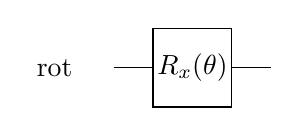
\begin{tikzpicture}[scale=.5] \node[draw=none] at (-3.5, 0) {rot}; \draw (-2,0) -- (-1, 0); \draw (1, 0) -- (2, 0); \draw (-1,-1)--(-1,1)--(1,1)--(1,-1)--cycle; \node[draw=none] at (0, 0) {$R_x(\theta)$}; \end{tikzpicture} } \]


\begin{DoxyParams}[1]{Parameters}
\mbox{\tt in,out}  & {\em multi\+Qubit} & object representing the set of all qubits \\
\hline
\mbox{\tt in}  & {\em rot\+Qubit} & qubit to rotate \\
\hline
\mbox{\tt in}  & {\em angle} & angle by which to rotate in radians \\
\hline
\end{DoxyParams}

\begin{DoxyExceptions}{Exceptions}
{\em exit\+With\+Error} & if {\ttfamily rot\+Qubit} is outside \mbox{[}0, {\ttfamily multi\+Qubit.\+num\+Qubits}). \\
\hline
\end{DoxyExceptions}


Definition at line 434 of file Qu\+E\+S\+T.\+c.



References rotate\+Around\+Axis().


\begin{DoxyCode}
434                                                                    \{
435 
436     \mbox{\hyperlink{structVector}{Vector}} unitAxis = \{1, 0, 0\};
437     \mbox{\hyperlink{QuEST_8c_a8810423457803005fecd415f4299f40d}{rotateAroundAxis}}(multiQubit, rotQubit, angle, unitAxis);
438 \}
\end{DoxyCode}
\mbox{\Hypertarget{QuEST_8c_ace0d3592d38a990e81a434c4e9681500}\label{QuEST_8c_ace0d3592d38a990e81a434c4e9681500}} 
\index{Qu\+E\+S\+T.\+c@{Qu\+E\+S\+T.\+c}!rotateY@{rotateY}}
\index{rotateY@{rotateY}!Qu\+E\+S\+T.\+c@{Qu\+E\+S\+T.\+c}}
\paragraph{\texorpdfstring{rotate\+Y()}{rotateY()}}
{\footnotesize\ttfamily void rotateY (\begin{DoxyParamCaption}\item[{\mbox{\hyperlink{structMultiQubit}{Multi\+Qubit}}}]{multi\+Qubit,  }\item[{const int}]{rot\+Qubit,  }\item[{\mbox{\hyperlink{QuEST__precision_8h_a4b654506f18b8bfd61ad2a29a7e38c25}{R\+E\+AL}}}]{angle }\end{DoxyParamCaption})}



Rotate a single qubit by a given angle around the Y-\/axis of the Bloch-\/sphere. 

For angle $\theta$, applies \[ \begin{pmatrix} \cos\theta/2 & - \sin \theta/2\\ \sin \theta/2 & \cos \theta/2 \end{pmatrix} \] ~\newline
 \[ \setlength{\fboxrule}{0.01pt} \fbox{ 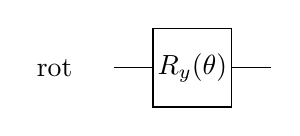
\begin{tikzpicture}[scale=.5] \node[draw=none] at (-3.5, 0) {rot}; \draw (-2,0) -- (-1, 0); \draw (1, 0) -- (2, 0); \draw (-1,-1)--(-1,1)--(1,1)--(1,-1)--cycle; \node[draw=none] at (0, 0) {$R_y(\theta)$}; \end{tikzpicture} } \]


\begin{DoxyParams}[1]{Parameters}
\mbox{\tt in,out}  & {\em multi\+Qubit} & object representing the set of all qubits \\
\hline
\mbox{\tt in}  & {\em rot\+Qubit} & qubit to rotate \\
\hline
\mbox{\tt in}  & {\em angle} & angle by which to rotate in radians \\
\hline
\end{DoxyParams}

\begin{DoxyExceptions}{Exceptions}
{\em exit\+With\+Error} & if {\ttfamily rot\+Qubit} is outside \mbox{[}0, {\ttfamily multi\+Qubit.\+num\+Qubits}). \\
\hline
\end{DoxyExceptions}


Definition at line 440 of file Qu\+E\+S\+T.\+c.



References rotate\+Around\+Axis().



Referenced by main().


\begin{DoxyCode}
440                                                                    \{
441 
442     \mbox{\hyperlink{structVector}{Vector}} unitAxis = \{0, 1, 0\};
443     \mbox{\hyperlink{QuEST_8c_a8810423457803005fecd415f4299f40d}{rotateAroundAxis}}(multiQubit, rotQubit, angle, unitAxis);
444 \}
\end{DoxyCode}
\mbox{\Hypertarget{QuEST_8c_abd621412ad30c1b034f4ce153c4afe10}\label{QuEST_8c_abd621412ad30c1b034f4ce153c4afe10}} 
\index{Qu\+E\+S\+T.\+c@{Qu\+E\+S\+T.\+c}!rotateZ@{rotateZ}}
\index{rotateZ@{rotateZ}!Qu\+E\+S\+T.\+c@{Qu\+E\+S\+T.\+c}}
\paragraph{\texorpdfstring{rotate\+Z()}{rotateZ()}}
{\footnotesize\ttfamily void rotateZ (\begin{DoxyParamCaption}\item[{\mbox{\hyperlink{structMultiQubit}{Multi\+Qubit}}}]{multi\+Qubit,  }\item[{const int}]{rot\+Qubit,  }\item[{\mbox{\hyperlink{QuEST__precision_8h_a4b654506f18b8bfd61ad2a29a7e38c25}{R\+E\+AL}}}]{angle }\end{DoxyParamCaption})}



Rotate a single qubit by a given angle around the Z-\/axis of the Bloch-\/sphere (also known as a phase shift gate). 

For angle $\theta$, applies \[ \begin{pmatrix} \exp(-i \theta/2) & 0 \\ 0 & \exp(i \theta/2) \end{pmatrix} \]

\[ \setlength{\fboxrule}{0.01pt} \fbox{ 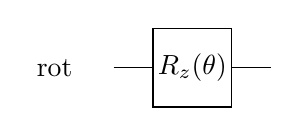
\begin{tikzpicture}[scale=.5] \node[draw=none] at (-3.5, 0) {rot}; \draw (-2,0) -- (-1, 0); \draw (1, 0) -- (2, 0); \draw (-1,-1)--(-1,1)--(1,1)--(1,-1)--cycle; \node[draw=none] at (0, 0) {$R_z(\theta)$}; \end{tikzpicture} } \]


\begin{DoxyParams}[1]{Parameters}
\mbox{\tt in,out}  & {\em multi\+Qubit} & object representing the set of all qubits \\
\hline
\mbox{\tt in}  & {\em rot\+Qubit} & qubit to rotate \\
\hline
\mbox{\tt in}  & {\em angle} & angle by which to rotate in radians \\
\hline
\end{DoxyParams}

\begin{DoxyExceptions}{Exceptions}
{\em exit\+With\+Error} & if {\ttfamily rot\+Qubit} is outside \mbox{[}0, {\ttfamily multi\+Qubit.\+num\+Qubits}). \\
\hline
\end{DoxyExceptions}


Definition at line 446 of file Qu\+E\+S\+T.\+c.



References rotate\+Around\+Axis().


\begin{DoxyCode}
446                                                                    \{
447 
448     \mbox{\hyperlink{structVector}{Vector}} unitAxis = \{0, 0, 1\};
449     \mbox{\hyperlink{QuEST_8c_a8810423457803005fecd415f4299f40d}{rotateAroundAxis}}(multiQubit, rotQubit, angle, unitAxis);
450 \}
\end{DoxyCode}
\mbox{\Hypertarget{QuEST_8c_adda6c47876a7676488ed0565a19eaa65}\label{QuEST_8c_adda6c47876a7676488ed0565a19eaa65}} 
\index{Qu\+E\+S\+T.\+c@{Qu\+E\+S\+T.\+c}!s\+Gate@{s\+Gate}}
\index{s\+Gate@{s\+Gate}!Qu\+E\+S\+T.\+c@{Qu\+E\+S\+T.\+c}}
\paragraph{\texorpdfstring{s\+Gate()}{sGate()}}
{\footnotesize\ttfamily void s\+Gate (\begin{DoxyParamCaption}\item[{\mbox{\hyperlink{structMultiQubit}{Multi\+Qubit}}}]{multi\+Qubit,  }\item[{const int}]{target\+Qubit }\end{DoxyParamCaption})}



Apply the single-\/qubit S gate. 

This is a rotation of $\pi/2$ around the Z-\/axis on the Bloch sphere, or the unitary\+: \[ \begin{pmatrix} 1 & 0 \\ 0 & i \end{pmatrix} \]

\[ \setlength{\fboxrule}{0.01pt} \fbox{ 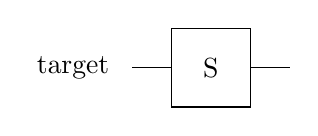
\begin{tikzpicture}[scale=.5] \node[draw=none] at (-3.5, 0) {target}; \draw (-2,0) -- (-1, 0); \draw (1, 0) -- (2, 0); \draw (-1,-1)--(-1,1)--(1,1)--(1,-1)--cycle; \node[draw=none] at (0, 0) {S}; \end{tikzpicture} } \]


\begin{DoxyParams}[1]{Parameters}
\mbox{\tt in,out}  & {\em multi\+Qubit} & object representing the set of all qubits \\
\hline
\mbox{\tt in}  & {\em target\+Qubit} & qubit to operate upon \\
\hline
\end{DoxyParams}

\begin{DoxyExceptions}{Exceptions}
{\em exit\+With\+Error} & if {\ttfamily target\+Qubit} is outside \mbox{[}0, {\ttfamily multi\+Qubit.\+num\+Qubits}) \\
\hline
\end{DoxyExceptions}


Definition at line 1619 of file Qu\+E\+S\+T.\+c.



References phase\+Gate(), and S\+\_\+\+G\+A\+TE.


\begin{DoxyCode}
1620 \{
1621     \mbox{\hyperlink{QuEST__env__local_8c_aae7a8a7f1ccbddb7f76b6c52b746bb43}{phaseGate}}(multiQubit, targetQubit, \mbox{\hyperlink{QuEST_8h_a5739021c733cecc49647956b2f7338eaa06e60f80fa80cce271793d6d31bcc21f}{S\_GATE}});
1622 \} 
\end{DoxyCode}
\mbox{\Hypertarget{QuEST_8c_a2275fff50824fe47485890ff5a857785}\label{QuEST_8c_a2275fff50824fe47485890ff5a857785}} 
\index{Qu\+E\+S\+T.\+c@{Qu\+E\+S\+T.\+c}!sigma\+X\+Distributed@{sigma\+X\+Distributed}}
\index{sigma\+X\+Distributed@{sigma\+X\+Distributed}!Qu\+E\+S\+T.\+c@{Qu\+E\+S\+T.\+c}}
\paragraph{\texorpdfstring{sigma\+X\+Distributed()}{sigmaXDistributed()}}
{\footnotesize\ttfamily void sigma\+X\+Distributed (\begin{DoxyParamCaption}\item[{\mbox{\hyperlink{structMultiQubit}{Multi\+Qubit}}}]{multi\+Qubit,  }\item[{const int}]{target\+Qubit,  }\item[{\mbox{\hyperlink{structComplexArray}{Complex\+Array}}}]{state\+Vec\+In,  }\item[{\mbox{\hyperlink{structComplexArray}{Complex\+Array}}}]{state\+Vec\+Out }\end{DoxyParamCaption})}



Rotate a single qubit by \{\{0,1\},\{1,0\}. 

Operate on a subset of the state vector with upper and lower block values stored seperately. This rotation is just swapping upper and lower values, and state\+Vec\+In must already be the correct section for this chunk

\begin{DoxyRemark}{Remarks}
Qubits are zero-\/based and the ~\newline
the first qubit is the rightmost ~\newline
 
\end{DoxyRemark}

\begin{DoxyParams}[1]{Parameters}
\mbox{\tt in,out}  & {\em multi\+Qubit} & object representing the set of qubits \\
\hline
\mbox{\tt in}  & {\em target\+Qubit} & qubit to rotate \\
\hline
\mbox{\tt in}  & {\em state\+Vec\+In} & probability amplitudes in lower or upper half of a block depending on chunk\+Id \\
\hline
\mbox{\tt out}  & {\em state\+Vec\+Out} & array section to update (will correspond to either the lower or upper half of a block) \\
\hline
\end{DoxyParams}


Definition at line 1158 of file Qu\+E\+S\+T.\+c.



References Complex\+Array\+::imag, Multi\+Qubit\+::num\+Amps, Complex\+Array\+::real, and R\+E\+AL.



Referenced by sigma\+X().


\begin{DoxyCode}
1161 \{
1162 
1163     \textcolor{keywordtype}{long} \textcolor{keywordtype}{long} \textcolor{keywordtype}{int} thisTask;  
1164     \textcolor{keyword}{const} \textcolor{keywordtype}{long} \textcolor{keywordtype}{long} \textcolor{keywordtype}{int} numTasks=multiQubit.\mbox{\hyperlink{structMultiQubit_ae16f47d8b725c914fb7f66b6498d79db}{numAmps}};
1165 
1166     \mbox{\hyperlink{QuEST__precision_8h_a4b654506f18b8bfd61ad2a29a7e38c25}{REAL}} *stateVecRealIn=stateVecIn.\mbox{\hyperlink{structComplexArray_a4195cac6c784ea1b6271f1c7dba1548a}{real}}, *stateVecImagIn=stateVecIn.
      \mbox{\hyperlink{structComplexArray_a79dde47c7ae530c79cebfdf57b225968}{imag}};
1167     \mbox{\hyperlink{QuEST__precision_8h_a4b654506f18b8bfd61ad2a29a7e38c25}{REAL}} *stateVecRealOut=stateVecOut.\mbox{\hyperlink{structComplexArray_a4195cac6c784ea1b6271f1c7dba1548a}{real}}, *stateVecImagOut=stateVecOut.
      \mbox{\hyperlink{structComplexArray_a79dde47c7ae530c79cebfdf57b225968}{imag}};
1168 
1169 \textcolor{preprocessor}{# ifdef \_OPENMP}
1170 \textcolor{preprocessor}{# pragma omp parallel \(\backslash\)}
1171 \textcolor{preprocessor}{    default  (none) \(\backslash\)}
1172 \textcolor{preprocessor}{    shared   (stateVecRealIn,stateVecImagIn,stateVecRealOut,stateVecImagOut) \(\backslash\)}
1173 \textcolor{preprocessor}{    private  (thisTask)}
1174 \textcolor{preprocessor}{# endif}
1175     \{
1176 \textcolor{preprocessor}{# ifdef \_OPENMP}
1177 \textcolor{preprocessor}{# pragma omp for schedule (static)}
1178 \textcolor{preprocessor}{# endif}
1179         \textcolor{keywordflow}{for} (thisTask=0; thisTask<numTasks; thisTask++) \{
1180             stateVecRealOut[thisTask] = stateVecRealIn[thisTask];
1181             stateVecImagOut[thisTask] = stateVecImagIn[thisTask];
1182         \}
1183     \}
1184 \} 
\end{DoxyCode}
\mbox{\Hypertarget{QuEST_8c_a74822fd86bb5d81766e6e8dbdcd62df1}\label{QuEST_8c_a74822fd86bb5d81766e6e8dbdcd62df1}} 
\index{Qu\+E\+S\+T.\+c@{Qu\+E\+S\+T.\+c}!sigma\+X\+Local@{sigma\+X\+Local}}
\index{sigma\+X\+Local@{sigma\+X\+Local}!Qu\+E\+S\+T.\+c@{Qu\+E\+S\+T.\+c}}
\paragraph{\texorpdfstring{sigma\+X\+Local()}{sigmaXLocal()}}
{\footnotesize\ttfamily void sigma\+X\+Local (\begin{DoxyParamCaption}\item[{\mbox{\hyperlink{structMultiQubit}{Multi\+Qubit}}}]{multi\+Qubit,  }\item[{const int}]{target\+Qubit }\end{DoxyParamCaption})}



Definition at line 1099 of file Qu\+E\+S\+T.\+c.



References Complex\+Array\+::imag, Multi\+Qubit\+::num\+Amps, Complex\+Array\+::real, R\+E\+AL, and Multi\+Qubit\+::state\+Vec.



Referenced by sigma\+X().


\begin{DoxyCode}
1100 \{
1101     \textcolor{keywordtype}{long} \textcolor{keywordtype}{long} \textcolor{keywordtype}{int} sizeBlock, sizeHalfBlock;
1102     \textcolor{keywordtype}{long} \textcolor{keywordtype}{long} \textcolor{keywordtype}{int} thisBlock, \textcolor{comment}{// current block}
1103          indexUp,indexLo;    \textcolor{comment}{// current index and corresponding index in lower half block}
1104 
1105     \mbox{\hyperlink{QuEST__precision_8h_a4b654506f18b8bfd61ad2a29a7e38c25}{REAL}} stateRealUp,stateImagUp;
1106     \textcolor{keywordtype}{long} \textcolor{keywordtype}{long} \textcolor{keywordtype}{int} thisTask;         
1107     \textcolor{keyword}{const} \textcolor{keywordtype}{long} \textcolor{keywordtype}{long} \textcolor{keywordtype}{int} numTasks=multiQubit.\mbox{\hyperlink{structMultiQubit_ae16f47d8b725c914fb7f66b6498d79db}{numAmps}}>>1;
1108 
1109     \textcolor{comment}{// set dimensions}
1110     sizeHalfBlock = 1LL << targetQubit;  
1111     sizeBlock     = 2LL * sizeHalfBlock; 
1112 
1113     \textcolor{comment}{// Can't use multiQubit.stateVec as a private OMP var}
1114     \mbox{\hyperlink{QuEST__precision_8h_a4b654506f18b8bfd61ad2a29a7e38c25}{REAL}} *stateVecReal = multiQubit.\mbox{\hyperlink{structMultiQubit_a45483190d6b01ef6b2f98f2bec9ab94f}{stateVec}}.\mbox{\hyperlink{structComplexArray_a4195cac6c784ea1b6271f1c7dba1548a}{real}};
1115     \mbox{\hyperlink{QuEST__precision_8h_a4b654506f18b8bfd61ad2a29a7e38c25}{REAL}} *stateVecImag = multiQubit.\mbox{\hyperlink{structMultiQubit_a45483190d6b01ef6b2f98f2bec9ab94f}{stateVec}}.\mbox{\hyperlink{structComplexArray_a79dde47c7ae530c79cebfdf57b225968}{imag}};
1116 
1117 \textcolor{preprocessor}{# ifdef \_OPENMP}
1118 \textcolor{preprocessor}{# pragma omp parallel \(\backslash\)}
1119 \textcolor{preprocessor}{    default  (none) \(\backslash\)}
1120 \textcolor{preprocessor}{    shared   (sizeBlock,sizeHalfBlock, stateVecReal,stateVecImag) \(\backslash\)}
1121 \textcolor{preprocessor}{    private  (thisTask,thisBlock ,indexUp,indexLo, stateRealUp,stateImagUp) }
1122 \textcolor{preprocessor}{# endif}
1123     \{
1124 \textcolor{preprocessor}{# ifdef \_OPENMP}
1125 \textcolor{preprocessor}{# pragma omp for schedule (static)}
1126 \textcolor{preprocessor}{# endif}
1127         \textcolor{keywordflow}{for} (thisTask=0; thisTask<numTasks; thisTask++) \{
1128             thisBlock   = thisTask / sizeHalfBlock;
1129             indexUp     = thisBlock*sizeBlock + thisTask%sizeHalfBlock;
1130             indexLo     = indexUp + sizeHalfBlock;
1131 
1132             stateRealUp = stateVecReal[indexUp];
1133             stateImagUp = stateVecImag[indexUp];
1134 
1135             stateVecReal[indexUp] = stateVecReal[indexLo];
1136             stateVecImag[indexUp] = stateVecImag[indexLo];
1137 
1138             stateVecReal[indexLo] = stateRealUp;
1139             stateVecImag[indexLo] = stateImagUp;
1140         \} 
1141     \}
1142 
1143 \}
\end{DoxyCode}
\mbox{\Hypertarget{QuEST_8c_af5ef5166f00c0572354b4ac53dcf40cf}\label{QuEST_8c_af5ef5166f00c0572354b4ac53dcf40cf}} 
\index{Qu\+E\+S\+T.\+c@{Qu\+E\+S\+T.\+c}!sigma\+Y\+Distributed@{sigma\+Y\+Distributed}}
\index{sigma\+Y\+Distributed@{sigma\+Y\+Distributed}!Qu\+E\+S\+T.\+c@{Qu\+E\+S\+T.\+c}}
\paragraph{\texorpdfstring{sigma\+Y\+Distributed()}{sigmaYDistributed()}}
{\footnotesize\ttfamily void sigma\+Y\+Distributed (\begin{DoxyParamCaption}\item[{\mbox{\hyperlink{structMultiQubit}{Multi\+Qubit}}}]{multi\+Qubit,  }\item[{const int}]{target\+Qubit,  }\item[{\mbox{\hyperlink{structComplexArray}{Complex\+Array}}}]{state\+Vec\+In,  }\item[{\mbox{\hyperlink{structComplexArray}{Complex\+Array}}}]{state\+Vec\+Out,  }\item[{int}]{update\+Upper }\end{DoxyParamCaption})}



Rotate a single qubit by \{\{0,-\/i\},\{i,0\}. 

Operate on a subset of the state vector with upper and lower block values stored seperately. This rotation is just swapping upper and lower values, and state\+Vec\+In must already be the correct section for this chunk

\begin{DoxyRemark}{Remarks}
Qubits are zero-\/based and the ~\newline
the first qubit is the rightmost ~\newline
 
\end{DoxyRemark}

\begin{DoxyParams}[1]{Parameters}
\mbox{\tt in,out}  & {\em multi\+Qubit} & object representing the set of qubits \\
\hline
\mbox{\tt in}  & {\em target\+Qubit} & qubit to rotate \\
\hline
\mbox{\tt in}  & {\em state\+Vec\+In} & probability amplitudes in lower or upper half of a block depending on chunk\+Id \\
\hline
\mbox{\tt in}  & {\em update\+Upper} & flag, 1\+: updating upper values, 0\+: updating lower values in block \\
\hline
\mbox{\tt out}  & {\em state\+Vec\+Out} & array section to update (will correspond to either the lower or upper half of a block) \\
\hline
\end{DoxyParams}


Definition at line 1345 of file Qu\+E\+S\+T.\+c.



References Complex\+Array\+::imag, Multi\+Qubit\+::num\+Amps, Complex\+Array\+::real, and R\+E\+AL.



Referenced by sigma\+Y().


\begin{DoxyCode}
1349 \{
1350 
1351     \textcolor{keywordtype}{long} \textcolor{keywordtype}{long} \textcolor{keywordtype}{int} thisTask;  
1352     \textcolor{keyword}{const} \textcolor{keywordtype}{long} \textcolor{keywordtype}{long} \textcolor{keywordtype}{int} numTasks=multiQubit.\mbox{\hyperlink{structMultiQubit_ae16f47d8b725c914fb7f66b6498d79db}{numAmps}};
1353 
1354     \mbox{\hyperlink{QuEST__precision_8h_a4b654506f18b8bfd61ad2a29a7e38c25}{REAL}} *stateVecRealIn=stateVecIn.\mbox{\hyperlink{structComplexArray_a4195cac6c784ea1b6271f1c7dba1548a}{real}}, *stateVecImagIn=stateVecIn.
      \mbox{\hyperlink{structComplexArray_a79dde47c7ae530c79cebfdf57b225968}{imag}};
1355     \mbox{\hyperlink{QuEST__precision_8h_a4b654506f18b8bfd61ad2a29a7e38c25}{REAL}} *stateVecRealOut=stateVecOut.\mbox{\hyperlink{structComplexArray_a4195cac6c784ea1b6271f1c7dba1548a}{real}}, *stateVecImagOut=stateVecOut.
      \mbox{\hyperlink{structComplexArray_a79dde47c7ae530c79cebfdf57b225968}{imag}};
1356 
1357     \textcolor{keywordtype}{int} realSign=1, imagSign=1;
1358     \textcolor{keywordflow}{if} (updateUpper) imagSign=-1;
1359     \textcolor{keywordflow}{else} realSign = -1;
1360 
1361 \textcolor{preprocessor}{# ifdef \_OPENMP}
1362 \textcolor{preprocessor}{# pragma omp parallel \(\backslash\)}
1363 \textcolor{preprocessor}{    default  (none) \(\backslash\)}
1364 \textcolor{preprocessor}{    shared   (stateVecRealIn,stateVecImagIn,stateVecRealOut,stateVecImagOut,realSign,imagSign) \(\backslash\)}
1365 \textcolor{preprocessor}{    private  (thisTask)}
1366 \textcolor{preprocessor}{# endif}
1367     \{
1368 \textcolor{preprocessor}{# ifdef \_OPENMP}
1369 \textcolor{preprocessor}{# pragma omp for schedule (static)}
1370 \textcolor{preprocessor}{# endif}
1371         \textcolor{keywordflow}{for} (thisTask=0; thisTask<numTasks; thisTask++) \{
1372             stateVecRealOut[thisTask] = realSign*stateVecImagIn[thisTask];
1373             stateVecImagOut[thisTask] = imagSign*stateVecRealIn[thisTask];
1374         \}
1375     \}
1376 \} 
\end{DoxyCode}
\mbox{\Hypertarget{QuEST_8c_a81fbfaed65a742a7dfd622e17652245e}\label{QuEST_8c_a81fbfaed65a742a7dfd622e17652245e}} 
\index{Qu\+E\+S\+T.\+c@{Qu\+E\+S\+T.\+c}!sigma\+Y\+Local@{sigma\+Y\+Local}}
\index{sigma\+Y\+Local@{sigma\+Y\+Local}!Qu\+E\+S\+T.\+c@{Qu\+E\+S\+T.\+c}}
\paragraph{\texorpdfstring{sigma\+Y\+Local()}{sigmaYLocal()}}
{\footnotesize\ttfamily void sigma\+Y\+Local (\begin{DoxyParamCaption}\item[{\mbox{\hyperlink{structMultiQubit}{Multi\+Qubit}}}]{multi\+Qubit,  }\item[{const int}]{target\+Qubit }\end{DoxyParamCaption})}



Definition at line 1286 of file Qu\+E\+S\+T.\+c.



References Complex\+Array\+::imag, Multi\+Qubit\+::num\+Amps, Complex\+Array\+::real, R\+E\+AL, and Multi\+Qubit\+::state\+Vec.



Referenced by sigma\+Y().


\begin{DoxyCode}
1287 \{
1288     \textcolor{keywordtype}{long} \textcolor{keywordtype}{long} \textcolor{keywordtype}{int} sizeBlock, sizeHalfBlock;
1289     \textcolor{keywordtype}{long} \textcolor{keywordtype}{long} \textcolor{keywordtype}{int} thisBlock, \textcolor{comment}{// current block}
1290          indexUp,indexLo;    \textcolor{comment}{// current index and corresponding index in lower half block}
1291 
1292     \mbox{\hyperlink{QuEST__precision_8h_a4b654506f18b8bfd61ad2a29a7e38c25}{REAL}} stateRealUp,stateImagUp;
1293     \textcolor{keywordtype}{long} \textcolor{keywordtype}{long} \textcolor{keywordtype}{int} thisTask;         
1294     \textcolor{keyword}{const} \textcolor{keywordtype}{long} \textcolor{keywordtype}{long} \textcolor{keywordtype}{int} numTasks=multiQubit.\mbox{\hyperlink{structMultiQubit_ae16f47d8b725c914fb7f66b6498d79db}{numAmps}}>>1;
1295 
1296     \textcolor{comment}{// set dimensions}
1297     sizeHalfBlock = 1LL << targetQubit;  
1298     sizeBlock     = 2LL * sizeHalfBlock; 
1299 
1300     \textcolor{comment}{// Can't use multiQubit.stateVec as a private OMP var}
1301     \mbox{\hyperlink{QuEST__precision_8h_a4b654506f18b8bfd61ad2a29a7e38c25}{REAL}} *stateVecReal = multiQubit.\mbox{\hyperlink{structMultiQubit_a45483190d6b01ef6b2f98f2bec9ab94f}{stateVec}}.\mbox{\hyperlink{structComplexArray_a4195cac6c784ea1b6271f1c7dba1548a}{real}};
1302     \mbox{\hyperlink{QuEST__precision_8h_a4b654506f18b8bfd61ad2a29a7e38c25}{REAL}} *stateVecImag = multiQubit.\mbox{\hyperlink{structMultiQubit_a45483190d6b01ef6b2f98f2bec9ab94f}{stateVec}}.\mbox{\hyperlink{structComplexArray_a79dde47c7ae530c79cebfdf57b225968}{imag}};
1303 
1304 \textcolor{preprocessor}{# ifdef \_OPENMP}
1305 \textcolor{preprocessor}{# pragma omp parallel \(\backslash\)}
1306 \textcolor{preprocessor}{    default  (none) \(\backslash\)}
1307 \textcolor{preprocessor}{    shared   (sizeBlock,sizeHalfBlock, stateVecReal,stateVecImag) \(\backslash\)}
1308 \textcolor{preprocessor}{    private  (thisTask,thisBlock ,indexUp,indexLo, stateRealUp,stateImagUp) }
1309 \textcolor{preprocessor}{# endif}
1310     \{
1311 \textcolor{preprocessor}{# ifdef \_OPENMP}
1312 \textcolor{preprocessor}{# pragma omp for schedule (static)}
1313 \textcolor{preprocessor}{# endif}
1314         \textcolor{keywordflow}{for} (thisTask=0; thisTask<numTasks; thisTask++) \{
1315             thisBlock   = thisTask / sizeHalfBlock;
1316             indexUp     = thisBlock*sizeBlock + thisTask%sizeHalfBlock;
1317             indexLo     = indexUp + sizeHalfBlock;
1318 
1319             stateRealUp = stateVecReal[indexUp];
1320             stateImagUp = stateVecImag[indexUp];
1321 
1322             stateVecReal[indexUp] = stateVecImag[indexLo];
1323             stateVecImag[indexUp] = -stateVecReal[indexLo];
1324 
1325             stateVecReal[indexLo] = -stateImagUp;
1326             stateVecImag[indexLo] = stateRealUp;
1327         \} 
1328     \}
1329 \}
\end{DoxyCode}
\mbox{\Hypertarget{QuEST_8c_aebaab86326779de55d335cfea3efde8f}\label{QuEST_8c_aebaab86326779de55d335cfea3efde8f}} 
\index{Qu\+E\+S\+T.\+c@{Qu\+E\+S\+T.\+c}!sigmaZ@{sigmaZ}}
\index{sigmaZ@{sigmaZ}!Qu\+E\+S\+T.\+c@{Qu\+E\+S\+T.\+c}}
\paragraph{\texorpdfstring{sigma\+Z()}{sigmaZ()}}
{\footnotesize\ttfamily void sigmaZ (\begin{DoxyParamCaption}\item[{\mbox{\hyperlink{structMultiQubit}{Multi\+Qubit}}}]{multi\+Qubit,  }\item[{const int}]{target\+Qubit }\end{DoxyParamCaption})}



Apply the single-\/qubit sigma-\/Z (also known as the Z, Pauli-\/Z or phase-\/flip) gate. 

This is a rotation of $\pi$ around the Z-\/axis (a phase shift) on the Bloch sphere. I.\+e. \[ \begin{pmatrix} 1 & 0 \\ 0 & -1 \end{pmatrix} \] ~\newline
 \[ \setlength{\fboxrule}{0.01pt} \fbox{ 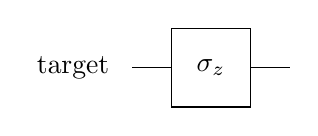
\begin{tikzpicture}[scale=.5] \node[draw=none] at (-3.5, 0) {target}; \draw (-2,0) -- (-1, 0); \draw (1, 0) -- (2, 0); \draw (-1,-1)--(-1,1)--(1,1)--(1,-1)--cycle; \node[draw=none] at (0, 0) {$\sigma_z$}; \end{tikzpicture} } \] ~\newline
 
\begin{DoxyParams}[1]{Parameters}
\mbox{\tt in,out}  & {\em multi\+Qubit} & object representing the set of all qubits \\
\hline
\mbox{\tt in}  & {\em target\+Qubit} & qubit to operate on \\
\hline
\end{DoxyParams}

\begin{DoxyExceptions}{Exceptions}
{\em exit\+With\+Error} & if {\ttfamily target\+Qubit} is outside \mbox{[}0, {\ttfamily multi\+Qubit.\+num\+Qubits}). \\
\hline
\end{DoxyExceptions}


Definition at line 1614 of file Qu\+E\+S\+T.\+c.



References phase\+Gate(), and S\+I\+G\+M\+A\+\_\+Z.


\begin{DoxyCode}
1615 \{
1616     \mbox{\hyperlink{QuEST__env__local_8c_aae7a8a7f1ccbddb7f76b6c52b746bb43}{phaseGate}}(multiQubit, targetQubit, \mbox{\hyperlink{QuEST_8h_a5739021c733cecc49647956b2f7338eaa754922d1e1846a1961ff2bf163483dac}{SIGMA\_Z}});
1617 \}
\end{DoxyCode}
\mbox{\Hypertarget{QuEST_8c_af764ea63a2e870098f4e1ce08562942e}\label{QuEST_8c_af764ea63a2e870098f4e1ce08562942e}} 
\index{Qu\+E\+S\+T.\+c@{Qu\+E\+S\+T.\+c}!t\+Gate@{t\+Gate}}
\index{t\+Gate@{t\+Gate}!Qu\+E\+S\+T.\+c@{Qu\+E\+S\+T.\+c}}
\paragraph{\texorpdfstring{t\+Gate()}{tGate()}}
{\footnotesize\ttfamily void t\+Gate (\begin{DoxyParamCaption}\item[{\mbox{\hyperlink{structMultiQubit}{Multi\+Qubit}}}]{multi\+Qubit,  }\item[{const int}]{target\+Qubit }\end{DoxyParamCaption})}



Apply the single-\/qubit T gate. 

This is a rotation of $\pi/4$ around the Z-\/axis on the Bloch sphere, or the unitary\+: \[ \begin{pmatrix} 1 & 0 \\ 0 & \exp\left(i \frac{\pi}{4}\right) \end{pmatrix} \]

\[ \setlength{\fboxrule}{0.01pt} \fbox{ 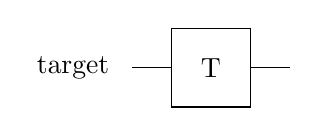
\begin{tikzpicture}[scale=.5] \node[draw=none] at (-3.5, 0) {target}; \draw (-2,0) -- (-1, 0); \draw (1, 0) -- (2, 0); \draw (-1,-1)--(-1,1)--(1,1)--(1,-1)--cycle; \node[draw=none] at (0, 0) {T}; \end{tikzpicture} } \]


\begin{DoxyParams}[1]{Parameters}
\mbox{\tt in,out}  & {\em multi\+Qubit} & object representing the set of all qubits \\
\hline
\mbox{\tt in}  & {\em target\+Qubit} & qubit to operate upon \\
\hline
\end{DoxyParams}

\begin{DoxyExceptions}{Exceptions}
{\em exit\+With\+Error} & if {\ttfamily target\+Qubit} is outside \mbox{[}0, {\ttfamily multi\+Qubit.\+num\+Qubits}) \\
\hline
\end{DoxyExceptions}


Definition at line 1624 of file Qu\+E\+S\+T.\+c.



References phase\+Gate(), and T\+\_\+\+G\+A\+TE.


\begin{DoxyCode}
1625 \{
1626     \mbox{\hyperlink{QuEST__env__local_8c_aae7a8a7f1ccbddb7f76b6c52b746bb43}{phaseGate}}(multiQubit, targetQubit, \mbox{\hyperlink{QuEST_8h_a5739021c733cecc49647956b2f7338eaa614d07d597a8e320cc556bc0e652e4ab}{T\_GATE}});
1627 \}
\end{DoxyCode}
\mbox{\Hypertarget{QuEST_8c_a2343b7240118e89aa615e2c9140b770b}\label{QuEST_8c_a2343b7240118e89aa615e2c9140b770b}} 
\index{Qu\+E\+S\+T.\+c@{Qu\+E\+S\+T.\+c}!unitary\+Distributed@{unitary\+Distributed}}
\index{unitary\+Distributed@{unitary\+Distributed}!Qu\+E\+S\+T.\+c@{Qu\+E\+S\+T.\+c}}
\paragraph{\texorpdfstring{unitary\+Distributed()}{unitaryDistributed()}}
{\footnotesize\ttfamily void unitary\+Distributed (\begin{DoxyParamCaption}\item[{\mbox{\hyperlink{structMultiQubit}{Multi\+Qubit}}}]{multi\+Qubit,  }\item[{const int}]{target\+Qubit,  }\item[{\mbox{\hyperlink{structComplex}{Complex}}}]{rot1,  }\item[{\mbox{\hyperlink{structComplex}{Complex}}}]{rot2,  }\item[{\mbox{\hyperlink{structComplexArray}{Complex\+Array}}}]{state\+Vec\+Up,  }\item[{\mbox{\hyperlink{structComplexArray}{Complex\+Array}}}]{state\+Vec\+Lo,  }\item[{\mbox{\hyperlink{structComplexArray}{Complex\+Array}}}]{state\+Vec\+Out }\end{DoxyParamCaption})}



Apply a unitary operation to a single qubit given a subset of the state vector with upper and lower block values stored seperately. 

\begin{DoxyRemark}{Remarks}
Qubits are zero-\/based and the first qubit is the rightmost ~\newline
 
\end{DoxyRemark}

\begin{DoxyParams}[1]{Parameters}
\mbox{\tt in,out}  & {\em multi\+Qubit} & object representing the set of qubits \\
\hline
\mbox{\tt in}  & {\em target\+Qubit} & qubit to rotate \\
\hline
\mbox{\tt in}  & {\em u} & unitary matrix to apply \\
\hline
\mbox{\tt in}  & {\em state\+Vec\+Up} & probability amplitudes in upper half of a block \\
\hline
\mbox{\tt in}  & {\em state\+Vec\+Lo} & probability amplitudes in lower half of a block \\
\hline
\mbox{\tt out}  & {\em state\+Vec\+Out} & array section to update (will correspond to either the lower or upper half of a block) \\
\hline
\end{DoxyParams}


Definition at line 668 of file Qu\+E\+S\+T.\+c.



References Complex\+Array\+::imag, Complex\+::imag, Multi\+Qubit\+::num\+Amps, Complex\+Array\+::real, Complex\+::real, and R\+E\+AL.



Referenced by unitary().


\begin{DoxyCode}
673 \{
674 
675     \mbox{\hyperlink{QuEST__precision_8h_a4b654506f18b8bfd61ad2a29a7e38c25}{REAL}}   stateRealUp,stateRealLo,stateImagUp,stateImagLo;
676     \textcolor{keywordtype}{long} \textcolor{keywordtype}{long} \textcolor{keywordtype}{int} thisTask;  
677     \textcolor{keyword}{const} \textcolor{keywordtype}{long} \textcolor{keywordtype}{long} \textcolor{keywordtype}{int} numTasks=multiQubit.\mbox{\hyperlink{structMultiQubit_ae16f47d8b725c914fb7f66b6498d79db}{numAmps}};
678 
679     \mbox{\hyperlink{QuEST__precision_8h_a4b654506f18b8bfd61ad2a29a7e38c25}{REAL}} rot1Real=rot1.\mbox{\hyperlink{structComplex_a479ad939835457595fcca3ca55c06283}{real}}, rot1Imag=rot1.\mbox{\hyperlink{structComplex_a1151948284b21c0052f203f23ab931d9}{imag}};
680     \mbox{\hyperlink{QuEST__precision_8h_a4b654506f18b8bfd61ad2a29a7e38c25}{REAL}} rot2Real=rot2.\mbox{\hyperlink{structComplex_a479ad939835457595fcca3ca55c06283}{real}}, rot2Imag=rot2.\mbox{\hyperlink{structComplex_a1151948284b21c0052f203f23ab931d9}{imag}};
681     \mbox{\hyperlink{QuEST__precision_8h_a4b654506f18b8bfd61ad2a29a7e38c25}{REAL}} *stateVecRealUp=stateVecUp.\mbox{\hyperlink{structComplexArray_a4195cac6c784ea1b6271f1c7dba1548a}{real}}, *stateVecImagUp=stateVecUp.
      \mbox{\hyperlink{structComplexArray_a79dde47c7ae530c79cebfdf57b225968}{imag}};
682     \mbox{\hyperlink{QuEST__precision_8h_a4b654506f18b8bfd61ad2a29a7e38c25}{REAL}} *stateVecRealLo=stateVecLo.\mbox{\hyperlink{structComplexArray_a4195cac6c784ea1b6271f1c7dba1548a}{real}}, *stateVecImagLo=stateVecLo.
      \mbox{\hyperlink{structComplexArray_a79dde47c7ae530c79cebfdf57b225968}{imag}};
683     \mbox{\hyperlink{QuEST__precision_8h_a4b654506f18b8bfd61ad2a29a7e38c25}{REAL}} *stateVecRealOut=stateVecOut.\mbox{\hyperlink{structComplexArray_a4195cac6c784ea1b6271f1c7dba1548a}{real}}, *stateVecImagOut=stateVecOut.
      \mbox{\hyperlink{structComplexArray_a79dde47c7ae530c79cebfdf57b225968}{imag}};
684 
685 
686 \textcolor{preprocessor}{# ifdef \_OPENMP}
687 \textcolor{preprocessor}{# pragma omp parallel \(\backslash\)}
688 \textcolor{preprocessor}{    default  (none) \(\backslash\)}
689 \textcolor{preprocessor}{    shared   (stateVecRealUp,stateVecImagUp,stateVecRealLo,stateVecImagLo,stateVecRealOut,stateVecImagOut, 
      \(\backslash\)}
690 \textcolor{preprocessor}{            rot1Real, rot1Imag, rot2Real, rot2Imag) \(\backslash\)}
691 \textcolor{preprocessor}{    private  (thisTask,stateRealUp,stateImagUp,stateRealLo,stateImagLo)}
692 \textcolor{preprocessor}{# endif}
693     \{
694 \textcolor{preprocessor}{# ifdef \_OPENMP}
695 \textcolor{preprocessor}{# pragma omp for schedule (static)}
696 \textcolor{preprocessor}{# endif}
697         \textcolor{keywordflow}{for} (thisTask=0; thisTask<numTasks; thisTask++) \{
698             \textcolor{comment}{// store current state vector values in temp variables}
699             stateRealUp = stateVecRealUp[thisTask];
700             stateImagUp = stateVecImagUp[thisTask];
701 
702             stateRealLo = stateVecRealLo[thisTask];
703             stateImagLo = stateVecImagLo[thisTask];
704 
705             stateVecRealOut[thisTask] = rot1Real*stateRealUp - rot1Imag*stateImagUp 
706                 + rot2Real*stateRealLo - rot2Imag*stateImagLo;
707             stateVecImagOut[thisTask] = rot1Real*stateImagUp + rot1Imag*stateRealUp 
708                 + rot2Real*stateImagLo + rot2Imag*stateRealLo;
709         \}
710     \}
711 \}
\end{DoxyCode}
\mbox{\Hypertarget{QuEST_8c_ac134fb45b0a7248c5d15e16eb7139a35}\label{QuEST_8c_ac134fb45b0a7248c5d15e16eb7139a35}} 
\index{Qu\+E\+S\+T.\+c@{Qu\+E\+S\+T.\+c}!unitary\+Local@{unitary\+Local}}
\index{unitary\+Local@{unitary\+Local}!Qu\+E\+S\+T.\+c@{Qu\+E\+S\+T.\+c}}
\paragraph{\texorpdfstring{unitary\+Local()}{unitaryLocal()}}
{\footnotesize\ttfamily void unitary\+Local (\begin{DoxyParamCaption}\item[{\mbox{\hyperlink{structMultiQubit}{Multi\+Qubit}}}]{multi\+Qubit,  }\item[{const int}]{target\+Qubit,  }\item[{\mbox{\hyperlink{structComplexMatrix2}{Complex\+Matrix2}}}]{u }\end{DoxyParamCaption})}



Definition at line 542 of file Qu\+E\+S\+T.\+c.



References Complex\+Array\+::imag, Complex\+::imag, Multi\+Qubit\+::num\+Amps, Complex\+Matrix2\+::r0c0, Complex\+Matrix2\+::r0c1, Complex\+Matrix2\+::r1c0, Complex\+Matrix2\+::r1c1, Complex\+Array\+::real, Complex\+::real, R\+E\+AL, and Multi\+Qubit\+::state\+Vec.



Referenced by unitary().


\begin{DoxyCode}
543 \{
544     \textcolor{keywordtype}{long} \textcolor{keywordtype}{long} \textcolor{keywordtype}{int} sizeBlock, sizeHalfBlock;
545     \textcolor{keywordtype}{long} \textcolor{keywordtype}{long} \textcolor{keywordtype}{int} thisBlock, \textcolor{comment}{// current block}
546          indexUp,indexLo;    \textcolor{comment}{// current index and corresponding index in lower half block}
547 
548     \mbox{\hyperlink{QuEST__precision_8h_a4b654506f18b8bfd61ad2a29a7e38c25}{REAL}} stateRealUp,stateRealLo,stateImagUp,stateImagLo;
549     \textcolor{keywordtype}{long} \textcolor{keywordtype}{long} \textcolor{keywordtype}{int} thisTask;         
550     \textcolor{keyword}{const} \textcolor{keywordtype}{long} \textcolor{keywordtype}{long} \textcolor{keywordtype}{int} numTasks=multiQubit.\mbox{\hyperlink{structMultiQubit_ae16f47d8b725c914fb7f66b6498d79db}{numAmps}}>>1;
551 
552     \textcolor{comment}{// set dimensions}
553     sizeHalfBlock = 1LL << targetQubit;  
554     sizeBlock     = 2LL * sizeHalfBlock; 
555 
556     \textcolor{comment}{// Can't use multiQubit.stateVec as a private OMP var}
557     \mbox{\hyperlink{QuEST__precision_8h_a4b654506f18b8bfd61ad2a29a7e38c25}{REAL}} *stateVecReal = multiQubit.\mbox{\hyperlink{structMultiQubit_a45483190d6b01ef6b2f98f2bec9ab94f}{stateVec}}.\mbox{\hyperlink{structComplexArray_a4195cac6c784ea1b6271f1c7dba1548a}{real}};
558     \mbox{\hyperlink{QuEST__precision_8h_a4b654506f18b8bfd61ad2a29a7e38c25}{REAL}} *stateVecImag = multiQubit.\mbox{\hyperlink{structMultiQubit_a45483190d6b01ef6b2f98f2bec9ab94f}{stateVec}}.\mbox{\hyperlink{structComplexArray_a79dde47c7ae530c79cebfdf57b225968}{imag}};
559 
560 \textcolor{preprocessor}{# ifdef \_OPENMP}
561 \textcolor{preprocessor}{# pragma omp parallel \(\backslash\)}
562 \textcolor{preprocessor}{    default  (none) \(\backslash\)}
563 \textcolor{preprocessor}{    shared   (sizeBlock,sizeHalfBlock, stateVecReal,stateVecImag, u) \(\backslash\)}
564 \textcolor{preprocessor}{    private  (thisTask,thisBlock ,indexUp,indexLo, stateRealUp,stateImagUp,stateRealLo,stateImagLo) }
565 \textcolor{preprocessor}{# endif}
566     \{
567 \textcolor{preprocessor}{# ifdef \_OPENMP}
568 \textcolor{preprocessor}{# pragma omp for schedule (static)}
569 \textcolor{preprocessor}{# endif}
570         \textcolor{keywordflow}{for} (thisTask=0; thisTask<numTasks; thisTask++) \{
571 
572             thisBlock   = thisTask / sizeHalfBlock;
573             indexUp     = thisBlock*sizeBlock + thisTask%sizeHalfBlock;
574             indexLo     = indexUp + sizeHalfBlock;
575 
576             \textcolor{comment}{// store current state vector values in temp variables}
577             stateRealUp = stateVecReal[indexUp];
578             stateImagUp = stateVecImag[indexUp];
579 
580             stateRealLo = stateVecReal[indexLo];
581             stateImagLo = stateVecImag[indexLo];
582 
583 
584             \textcolor{comment}{// state[indexUp] = u00 * state[indexUp] + u01 * state[indexLo]}
585             stateVecReal[indexUp] = u.\mbox{\hyperlink{structComplexMatrix2_ae72b4458233b077a636beee1892e81ff}{r0c0}}.\mbox{\hyperlink{structComplex_a479ad939835457595fcca3ca55c06283}{real}}*stateRealUp - u.\mbox{\hyperlink{structComplexMatrix2_ae72b4458233b077a636beee1892e81ff}{r0c0}}.
      \mbox{\hyperlink{structComplex_a1151948284b21c0052f203f23ab931d9}{imag}}*stateImagUp 
586                 + u.\mbox{\hyperlink{structComplexMatrix2_a0f3932f055a8b05cef361bce25d51172}{r0c1}}.\mbox{\hyperlink{structComplex_a479ad939835457595fcca3ca55c06283}{real}}*stateRealLo - u.\mbox{\hyperlink{structComplexMatrix2_a0f3932f055a8b05cef361bce25d51172}{r0c1}}.\mbox{\hyperlink{structComplex_a1151948284b21c0052f203f23ab931d9}{imag}}*stateImagLo;
587             stateVecImag[indexUp] = u.\mbox{\hyperlink{structComplexMatrix2_ae72b4458233b077a636beee1892e81ff}{r0c0}}.\mbox{\hyperlink{structComplex_a479ad939835457595fcca3ca55c06283}{real}}*stateImagUp + u.\mbox{\hyperlink{structComplexMatrix2_ae72b4458233b077a636beee1892e81ff}{r0c0}}.
      \mbox{\hyperlink{structComplex_a1151948284b21c0052f203f23ab931d9}{imag}}*stateRealUp 
588                 + u.\mbox{\hyperlink{structComplexMatrix2_a0f3932f055a8b05cef361bce25d51172}{r0c1}}.\mbox{\hyperlink{structComplex_a479ad939835457595fcca3ca55c06283}{real}}*stateImagLo + u.\mbox{\hyperlink{structComplexMatrix2_a0f3932f055a8b05cef361bce25d51172}{r0c1}}.\mbox{\hyperlink{structComplex_a1151948284b21c0052f203f23ab931d9}{imag}}*stateRealLo;
589 
590             \textcolor{comment}{// state[indexLo] = u10  * state[indexUp] + u11 * state[indexLo]}
591             stateVecReal[indexLo] = u.\mbox{\hyperlink{structComplexMatrix2_ab98282015ed2065e53fbc9638e2583ab}{r1c0}}.\mbox{\hyperlink{structComplex_a479ad939835457595fcca3ca55c06283}{real}}*stateRealUp  - u.\mbox{\hyperlink{structComplexMatrix2_ab98282015ed2065e53fbc9638e2583ab}{r1c0}}.
      \mbox{\hyperlink{structComplex_a1151948284b21c0052f203f23ab931d9}{imag}}*stateImagUp 
592                 + u.\mbox{\hyperlink{structComplexMatrix2_a763007c3070802373549ba0350f83c8a}{r1c1}}.\mbox{\hyperlink{structComplex_a479ad939835457595fcca3ca55c06283}{real}}*stateRealLo  -  u.\mbox{\hyperlink{structComplexMatrix2_a763007c3070802373549ba0350f83c8a}{r1c1}}.\mbox{\hyperlink{structComplex_a1151948284b21c0052f203f23ab931d9}{imag}}*stateImagLo;
593             stateVecImag[indexLo] = u.\mbox{\hyperlink{structComplexMatrix2_ab98282015ed2065e53fbc9638e2583ab}{r1c0}}.\mbox{\hyperlink{structComplex_a479ad939835457595fcca3ca55c06283}{real}}*stateImagUp + u.\mbox{\hyperlink{structComplexMatrix2_ab98282015ed2065e53fbc9638e2583ab}{r1c0}}.
      \mbox{\hyperlink{structComplex_a1151948284b21c0052f203f23ab931d9}{imag}}*stateRealUp 
594                 + u.\mbox{\hyperlink{structComplexMatrix2_a763007c3070802373549ba0350f83c8a}{r1c1}}.\mbox{\hyperlink{structComplex_a479ad939835457595fcca3ca55c06283}{real}}*stateImagLo + u.\mbox{\hyperlink{structComplexMatrix2_a763007c3070802373549ba0350f83c8a}{r1c1}}.\mbox{\hyperlink{structComplex_a1151948284b21c0052f203f23ab931d9}{imag}}*stateRealLo;
595 
596         \} 
597     \}
598 \} 
\end{DoxyCode}
\mbox{\Hypertarget{QuEST_8c_ae2b2c14a07dd7d50ff86032a3ca101d7}\label{QuEST_8c_ae2b2c14a07dd7d50ff86032a3ca101d7}} 
\index{Qu\+E\+S\+T.\+c@{Qu\+E\+S\+T.\+c}!validate\+Alpha\+Beta@{validate\+Alpha\+Beta}}
\index{validate\+Alpha\+Beta@{validate\+Alpha\+Beta}!Qu\+E\+S\+T.\+c@{Qu\+E\+S\+T.\+c}}
\paragraph{\texorpdfstring{validate\+Alpha\+Beta()}{validateAlphaBeta()}}
{\footnotesize\ttfamily int validate\+Alpha\+Beta (\begin{DoxyParamCaption}\item[{\mbox{\hyperlink{structComplex}{Complex}}}]{alpha,  }\item[{\mbox{\hyperlink{structComplex}{Complex}}}]{beta }\end{DoxyParamCaption})}



Definition at line 408 of file Qu\+E\+S\+T.\+c.



References Complex\+::imag, Complex\+::real, and R\+E\+A\+L\+\_\+\+E\+PS.



Referenced by compact\+Unitary(), and controlled\+Compact\+Unitary().


\begin{DoxyCode}
408                                                   \{
409     \textcolor{keywordflow}{if} ( fabs(alpha.\mbox{\hyperlink{structComplex_a479ad939835457595fcca3ca55c06283}{real}}*alpha.\mbox{\hyperlink{structComplex_a479ad939835457595fcca3ca55c06283}{real}} 
410                 + alpha.\mbox{\hyperlink{structComplex_a1151948284b21c0052f203f23ab931d9}{imag}}*alpha.\mbox{\hyperlink{structComplex_a1151948284b21c0052f203f23ab931d9}{imag}}
411                 + beta.\mbox{\hyperlink{structComplex_a479ad939835457595fcca3ca55c06283}{real}}*beta.\mbox{\hyperlink{structComplex_a479ad939835457595fcca3ca55c06283}{real}} 
412                 + beta.\mbox{\hyperlink{structComplex_a1151948284b21c0052f203f23ab931d9}{imag}}*beta.\mbox{\hyperlink{structComplex_a1151948284b21c0052f203f23ab931d9}{imag}} - 1) > \mbox{\hyperlink{QuEST__precision_8h_aebb5e6716e06431296af4d1a71744dec}{REAL\_EPS}} ) \textcolor{keywordflow}{return} 0;
413     \textcolor{keywordflow}{else} \textcolor{keywordflow}{return} 1;
414 \}
\end{DoxyCode}
\mbox{\Hypertarget{QuEST_8c_ae4fea133d1a8f09ff8da03038100adb2}\label{QuEST_8c_ae4fea133d1a8f09ff8da03038100adb2}} 
\index{Qu\+E\+S\+T.\+c@{Qu\+E\+S\+T.\+c}!validate\+Matrix\+Is\+Unitary@{validate\+Matrix\+Is\+Unitary}}
\index{validate\+Matrix\+Is\+Unitary@{validate\+Matrix\+Is\+Unitary}!Qu\+E\+S\+T.\+c@{Qu\+E\+S\+T.\+c}}
\paragraph{\texorpdfstring{validate\+Matrix\+Is\+Unitary()}{validateMatrixIsUnitary()}}
{\footnotesize\ttfamily int validate\+Matrix\+Is\+Unitary (\begin{DoxyParamCaption}\item[{\mbox{\hyperlink{structComplexMatrix2}{Complex\+Matrix2}}}]{u }\end{DoxyParamCaption})}



Definition at line 384 of file Qu\+E\+S\+T.\+c.



References Complex\+::imag, Complex\+Matrix2\+::r0c0, Complex\+Matrix2\+::r0c1, Complex\+Matrix2\+::r1c0, Complex\+Matrix2\+::r1c1, Complex\+::real, and R\+E\+A\+L\+\_\+\+E\+PS.



Referenced by controlled\+Unitary(), multi\+Controlled\+Unitary(), and unitary().


\begin{DoxyCode}
384                                              \{
385 
386     \textcolor{keywordflow}{if} ( fabs(u.\mbox{\hyperlink{structComplexMatrix2_ae72b4458233b077a636beee1892e81ff}{r0c0}}.\mbox{\hyperlink{structComplex_a479ad939835457595fcca3ca55c06283}{real}}*u.\mbox{\hyperlink{structComplexMatrix2_ae72b4458233b077a636beee1892e81ff}{r0c0}}.\mbox{\hyperlink{structComplex_a479ad939835457595fcca3ca55c06283}{real}} 
387                 + u.\mbox{\hyperlink{structComplexMatrix2_ae72b4458233b077a636beee1892e81ff}{r0c0}}.\mbox{\hyperlink{structComplex_a1151948284b21c0052f203f23ab931d9}{imag}}*u.\mbox{\hyperlink{structComplexMatrix2_ae72b4458233b077a636beee1892e81ff}{r0c0}}.\mbox{\hyperlink{structComplex_a1151948284b21c0052f203f23ab931d9}{imag}}
388                 + u.\mbox{\hyperlink{structComplexMatrix2_ab98282015ed2065e53fbc9638e2583ab}{r1c0}}.\mbox{\hyperlink{structComplex_a479ad939835457595fcca3ca55c06283}{real}}*u.\mbox{\hyperlink{structComplexMatrix2_ab98282015ed2065e53fbc9638e2583ab}{r1c0}}.\mbox{\hyperlink{structComplex_a479ad939835457595fcca3ca55c06283}{real}}
389                 + u.\mbox{\hyperlink{structComplexMatrix2_ab98282015ed2065e53fbc9638e2583ab}{r1c0}}.\mbox{\hyperlink{structComplex_a1151948284b21c0052f203f23ab931d9}{imag}}*u.\mbox{\hyperlink{structComplexMatrix2_ab98282015ed2065e53fbc9638e2583ab}{r1c0}}.\mbox{\hyperlink{structComplex_a1151948284b21c0052f203f23ab931d9}{imag}} - 1) > \mbox{\hyperlink{QuEST__precision_8h_aebb5e6716e06431296af4d1a71744dec}{REAL\_EPS}} ) \textcolor{keywordflow}{return} 0;
390     \textcolor{keywordflow}{if} ( fabs(u.\mbox{\hyperlink{structComplexMatrix2_a0f3932f055a8b05cef361bce25d51172}{r0c1}}.\mbox{\hyperlink{structComplex_a479ad939835457595fcca3ca55c06283}{real}}*u.\mbox{\hyperlink{structComplexMatrix2_a0f3932f055a8b05cef361bce25d51172}{r0c1}}.\mbox{\hyperlink{structComplex_a479ad939835457595fcca3ca55c06283}{real}} 
391                 + u.\mbox{\hyperlink{structComplexMatrix2_a0f3932f055a8b05cef361bce25d51172}{r0c1}}.\mbox{\hyperlink{structComplex_a1151948284b21c0052f203f23ab931d9}{imag}}*u.\mbox{\hyperlink{structComplexMatrix2_a0f3932f055a8b05cef361bce25d51172}{r0c1}}.\mbox{\hyperlink{structComplex_a1151948284b21c0052f203f23ab931d9}{imag}}
392                 + u.\mbox{\hyperlink{structComplexMatrix2_a763007c3070802373549ba0350f83c8a}{r1c1}}.\mbox{\hyperlink{structComplex_a479ad939835457595fcca3ca55c06283}{real}}*u.\mbox{\hyperlink{structComplexMatrix2_a763007c3070802373549ba0350f83c8a}{r1c1}}.\mbox{\hyperlink{structComplex_a479ad939835457595fcca3ca55c06283}{real}}
393                 + u.\mbox{\hyperlink{structComplexMatrix2_a763007c3070802373549ba0350f83c8a}{r1c1}}.\mbox{\hyperlink{structComplex_a1151948284b21c0052f203f23ab931d9}{imag}}*u.\mbox{\hyperlink{structComplexMatrix2_a763007c3070802373549ba0350f83c8a}{r1c1}}.\mbox{\hyperlink{structComplex_a1151948284b21c0052f203f23ab931d9}{imag}} - 1) > \mbox{\hyperlink{QuEST__precision_8h_aebb5e6716e06431296af4d1a71744dec}{REAL\_EPS}} ) \textcolor{keywordflow}{return} 0;
394 
395     \textcolor{keywordflow}{if} ( fabs(u.\mbox{\hyperlink{structComplexMatrix2_ae72b4458233b077a636beee1892e81ff}{r0c0}}.\mbox{\hyperlink{structComplex_a479ad939835457595fcca3ca55c06283}{real}}*u.\mbox{\hyperlink{structComplexMatrix2_a0f3932f055a8b05cef361bce25d51172}{r0c1}}.\mbox{\hyperlink{structComplex_a479ad939835457595fcca3ca55c06283}{real}} 
396                 + u.\mbox{\hyperlink{structComplexMatrix2_ae72b4458233b077a636beee1892e81ff}{r0c0}}.\mbox{\hyperlink{structComplex_a1151948284b21c0052f203f23ab931d9}{imag}}*u.\mbox{\hyperlink{structComplexMatrix2_a0f3932f055a8b05cef361bce25d51172}{r0c1}}.\mbox{\hyperlink{structComplex_a1151948284b21c0052f203f23ab931d9}{imag}}
397                 + u.\mbox{\hyperlink{structComplexMatrix2_ab98282015ed2065e53fbc9638e2583ab}{r1c0}}.\mbox{\hyperlink{structComplex_a479ad939835457595fcca3ca55c06283}{real}}*u.\mbox{\hyperlink{structComplexMatrix2_a763007c3070802373549ba0350f83c8a}{r1c1}}.\mbox{\hyperlink{structComplex_a479ad939835457595fcca3ca55c06283}{real}}
398                 + u.\mbox{\hyperlink{structComplexMatrix2_ab98282015ed2065e53fbc9638e2583ab}{r1c0}}.\mbox{\hyperlink{structComplex_a1151948284b21c0052f203f23ab931d9}{imag}}*u.\mbox{\hyperlink{structComplexMatrix2_a763007c3070802373549ba0350f83c8a}{r1c1}}.\mbox{\hyperlink{structComplex_a1151948284b21c0052f203f23ab931d9}{imag}}) > \mbox{\hyperlink{QuEST__precision_8h_aebb5e6716e06431296af4d1a71744dec}{REAL\_EPS}} ) \textcolor{keywordflow}{return} 0;
399 
400     \textcolor{keywordflow}{if} ( fabs(u.\mbox{\hyperlink{structComplexMatrix2_a0f3932f055a8b05cef361bce25d51172}{r0c1}}.\mbox{\hyperlink{structComplex_a479ad939835457595fcca3ca55c06283}{real}}*u.\mbox{\hyperlink{structComplexMatrix2_ae72b4458233b077a636beee1892e81ff}{r0c0}}.\mbox{\hyperlink{structComplex_a1151948284b21c0052f203f23ab931d9}{imag}}
401                 - u.\mbox{\hyperlink{structComplexMatrix2_ae72b4458233b077a636beee1892e81ff}{r0c0}}.\mbox{\hyperlink{structComplex_a479ad939835457595fcca3ca55c06283}{real}}*u.\mbox{\hyperlink{structComplexMatrix2_a0f3932f055a8b05cef361bce25d51172}{r0c1}}.\mbox{\hyperlink{structComplex_a1151948284b21c0052f203f23ab931d9}{imag}}
402                 + u.\mbox{\hyperlink{structComplexMatrix2_a763007c3070802373549ba0350f83c8a}{r1c1}}.\mbox{\hyperlink{structComplex_a479ad939835457595fcca3ca55c06283}{real}}*u.\mbox{\hyperlink{structComplexMatrix2_ab98282015ed2065e53fbc9638e2583ab}{r1c0}}.\mbox{\hyperlink{structComplex_a1151948284b21c0052f203f23ab931d9}{imag}}
403                 - u.\mbox{\hyperlink{structComplexMatrix2_ab98282015ed2065e53fbc9638e2583ab}{r1c0}}.\mbox{\hyperlink{structComplex_a479ad939835457595fcca3ca55c06283}{real}}*u.\mbox{\hyperlink{structComplexMatrix2_a763007c3070802373549ba0350f83c8a}{r1c1}}.\mbox{\hyperlink{structComplex_a1151948284b21c0052f203f23ab931d9}{imag}}) > \mbox{\hyperlink{QuEST__precision_8h_aebb5e6716e06431296af4d1a71744dec}{REAL\_EPS}} ) \textcolor{keywordflow}{return} 0;
404 
405     \textcolor{keywordflow}{return} 1;
406 \}
\end{DoxyCode}
\mbox{\Hypertarget{QuEST_8c_a71c14976f63cfcda70026fa20ee531fe}\label{QuEST_8c_a71c14976f63cfcda70026fa20ee531fe}} 
\index{Qu\+E\+S\+T.\+c@{Qu\+E\+S\+T.\+c}!validate\+Unit\+Vector@{validate\+Unit\+Vector}}
\index{validate\+Unit\+Vector@{validate\+Unit\+Vector}!Qu\+E\+S\+T.\+c@{Qu\+E\+S\+T.\+c}}
\paragraph{\texorpdfstring{validate\+Unit\+Vector()}{validateUnitVector()}}
{\footnotesize\ttfamily int validate\+Unit\+Vector (\begin{DoxyParamCaption}\item[{\mbox{\hyperlink{QuEST__precision_8h_a4b654506f18b8bfd61ad2a29a7e38c25}{R\+E\+AL}}}]{ux,  }\item[{\mbox{\hyperlink{QuEST__precision_8h_a4b654506f18b8bfd61ad2a29a7e38c25}{R\+E\+AL}}}]{uy,  }\item[{\mbox{\hyperlink{QuEST__precision_8h_a4b654506f18b8bfd61ad2a29a7e38c25}{R\+E\+AL}}}]{uz }\end{DoxyParamCaption})}



Definition at line 416 of file Qu\+E\+S\+T.\+c.



References R\+E\+A\+L\+\_\+\+E\+PS.


\begin{DoxyCode}
416                                                  \{
417     \textcolor{keywordflow}{if} ( fabs(sqrt(ux*ux + uy*uy + uz*uz) - 1) > \mbox{\hyperlink{QuEST__precision_8h_aebb5e6716e06431296af4d1a71744dec}{REAL\_EPS}} ) \textcolor{keywordflow}{return} 0;
418     \textcolor{keywordflow}{else} \textcolor{keywordflow}{return} 1;
419 \}
\end{DoxyCode}


\subsubsection{Variable Documentation}
\mbox{\Hypertarget{QuEST_8c_aac1637696885c75b73a1ecf381cea713}\label{QuEST_8c_aac1637696885c75b73a1ecf381cea713}} 
\index{Qu\+E\+S\+T.\+c@{Qu\+E\+S\+T.\+c}!error\+Codes@{error\+Codes}}
\index{error\+Codes@{error\+Codes}!Qu\+E\+S\+T.\+c@{Qu\+E\+S\+T.\+c}}
\paragraph{\texorpdfstring{error\+Codes}{errorCodes}}
{\footnotesize\ttfamily const char$\ast$ error\+Codes\mbox{[}$\,$\mbox{]}}

{\bfseries Initial value\+:}
\begin{DoxyCode}
= \{
    \textcolor{stringliteral}{"Success"},                                              
    \textcolor{stringliteral}{"Invalid target qubit. Note qubits are zero indexed."},  
    \textcolor{stringliteral}{"Invalid control qubit. Note qubits are zero indexed."}, 
    \textcolor{stringliteral}{"Control qubit cannot equal target qubit."},             
    \textcolor{stringliteral}{"Invalid number of control qubits"},                     
    \textcolor{stringliteral}{"Invalid unitary matrix."},                              
    \textcolor{stringliteral}{"Invalid rotation arguments."},                          
    \textcolor{stringliteral}{"Invalid system size. Cannot print output for systems greater than 5 qubits."}, 
    \textcolor{stringliteral}{"Can't collapse to state with zero probability."}, 
    \textcolor{stringliteral}{"Invalid number of qubits."}, 
    \textcolor{stringliteral}{"Invalid measurement outcome -- must be either 0 or 1."}, 
    \textcolor{stringliteral}{"Could not open file"} 
\}
\end{DoxyCode}


Definition at line 30 of file Qu\+E\+S\+T.\+c.



Referenced by exit\+With\+Error().


\hypertarget{QuEST_8h}{}\subsection{Qu\+E\+S\+T.\+h File Reference}
\label{QuEST_8h}\index{Qu\+E\+S\+T.\+h@{Qu\+E\+S\+T.\+h}}


The Qu\+E\+ST library A\+PI and objects.  


{\ttfamily \#include \char`\"{}Qu\+E\+S\+T\+\_\+precision.\+h\char`\"{}}\newline
\subsubsection*{Data Structures}
\begin{DoxyCompactItemize}
\item 
struct \mbox{\hyperlink{structComplex}{Complex}}
\begin{DoxyCompactList}\small\item\em Represents one complex number. \end{DoxyCompactList}\item 
struct \mbox{\hyperlink{structComplexArray}{Complex\+Array}}
\begin{DoxyCompactList}\small\item\em Represents an array of complex numbers grouped into an array of real components and an array of coressponding complex components. \end{DoxyCompactList}\item 
struct \mbox{\hyperlink{structComplexMatrix2}{Complex\+Matrix2}}
\begin{DoxyCompactList}\small\item\em Represents a 2x2 matrix of complex numbers. \end{DoxyCompactList}\item 
struct \mbox{\hyperlink{structMultiQubit}{Multi\+Qubit}}
\begin{DoxyCompactList}\small\item\em Represents a system of qubits. \end{DoxyCompactList}\item 
struct \mbox{\hyperlink{structQuESTEnv}{Qu\+E\+S\+T\+Env}}
\begin{DoxyCompactList}\small\item\em Information about the environment the program is running in. \end{DoxyCompactList}\item 
struct \mbox{\hyperlink{structVector}{Vector}}
\begin{DoxyCompactList}\small\item\em Represents a 3-\/vector of real numbers. \end{DoxyCompactList}\end{DoxyCompactItemize}
\subsubsection*{Typedefs}
\begin{DoxyCompactItemize}
\item 
typedef struct \mbox{\hyperlink{structComplex}{Complex}} \mbox{\hyperlink{QuEST_8h_ad59c9e471673c07782e6c403277ffd8d}{Complex}}
\begin{DoxyCompactList}\small\item\em Represents one complex number. \end{DoxyCompactList}\item 
typedef struct \mbox{\hyperlink{structComplexArray}{Complex\+Array}} \mbox{\hyperlink{QuEST_8h_a19e00739fde70a851d068f322cf915c8}{Complex\+Array}}
\begin{DoxyCompactList}\small\item\em Represents an array of complex numbers grouped into an array of real components and an array of coressponding complex components. \end{DoxyCompactList}\item 
typedef struct \mbox{\hyperlink{structComplexMatrix2}{Complex\+Matrix2}} \mbox{\hyperlink{QuEST_8h_aa6e00518bd2c71030c52d5955e506875}{Complex\+Matrix2}}
\begin{DoxyCompactList}\small\item\em Represents a 2x2 matrix of complex numbers. \end{DoxyCompactList}\item 
typedef struct \mbox{\hyperlink{structMultiQubit}{Multi\+Qubit}} \mbox{\hyperlink{QuEST_8h_af4123a681074068eeeee1562758eef61}{Multi\+Qubit}}
\begin{DoxyCompactList}\small\item\em Represents a system of qubits. \end{DoxyCompactList}\item 
typedef struct \mbox{\hyperlink{structQuESTEnv}{Qu\+E\+S\+T\+Env}} \mbox{\hyperlink{QuEST_8h_aedfe2bb713c31d6133e53b1bd72d7a2c}{Qu\+E\+S\+T\+Env}}
\begin{DoxyCompactList}\small\item\em Information about the environment the program is running in. \end{DoxyCompactList}\item 
typedef struct \mbox{\hyperlink{structVector}{Vector}} \mbox{\hyperlink{QuEST_8h_a6ded2cf071c127e518317e3c451af3ef}{Vector}}
\begin{DoxyCompactList}\small\item\em Represents a 3-\/vector of real numbers. \end{DoxyCompactList}\end{DoxyCompactItemize}
\subsubsection*{Enumerations}
\begin{DoxyCompactItemize}
\item 
enum \mbox{\hyperlink{QuEST_8h_a5739021c733cecc49647956b2f7338ea}{phase\+Gate\+Type}} \{ \mbox{\hyperlink{QuEST_8h_a5739021c733cecc49647956b2f7338eaa754922d1e1846a1961ff2bf163483dac}{S\+I\+G\+M\+A\+\_\+Z}} =0, 
\mbox{\hyperlink{QuEST_8h_a5739021c733cecc49647956b2f7338eaa06e60f80fa80cce271793d6d31bcc21f}{S\+\_\+\+G\+A\+TE}} =1, 
\mbox{\hyperlink{QuEST_8h_a5739021c733cecc49647956b2f7338eaa614d07d597a8e320cc556bc0e652e4ab}{T\+\_\+\+G\+A\+TE}} =2
 \}
\end{DoxyCompactItemize}
\subsubsection*{Functions}
\begin{DoxyCompactItemize}
\item 
\mbox{\hyperlink{QuEST__precision_8h_a4b654506f18b8bfd61ad2a29a7e38c25}{R\+E\+AL}} \mbox{\hyperlink{QuEST_8h_a818a4c7cd7252d2b10b896b12fa431d3}{calc\+Total\+Probability}} (\mbox{\hyperlink{structMultiQubit}{Multi\+Qubit}} multi\+Qubit)
\begin{DoxyCompactList}\small\item\em Calculate the probability of being in any state by taking the norm of the entire state vector. \end{DoxyCompactList}\item 
void \mbox{\hyperlink{QuEST_8h_abd4bc926cd3f9b65610bb228d0c59fe0}{close\+Qu\+E\+S\+T\+Env}} (\mbox{\hyperlink{structQuESTEnv}{Qu\+E\+S\+T\+Env}} env)
\begin{DoxyCompactList}\small\item\em Close Qu\+E\+ST environment. \end{DoxyCompactList}\item 
\mbox{\hyperlink{QuEST__precision_8h_a4b654506f18b8bfd61ad2a29a7e38c25}{R\+E\+AL}} \mbox{\hyperlink{QuEST_8h_a07418ebac70fd9ae5d051d089961631d}{collapse\+To\+Outcome}} (\mbox{\hyperlink{structMultiQubit}{Multi\+Qubit}} multi\+Qubit, const int measure\+Qubit, int outcome)
\begin{DoxyCompactList}\small\item\em Updates the state vector to be consistent with measuring the measure qubit in the given outcome (0 or 1), and returns the probability of such a measurement outcome. \end{DoxyCompactList}\item 
void \mbox{\hyperlink{QuEST_8h_a03b13dfcabd8c59b50dbdd3af44ba8b2}{compact\+Unitary}} (\mbox{\hyperlink{structMultiQubit}{Multi\+Qubit}} multi\+Qubit, const int target\+Qubit, \mbox{\hyperlink{structComplex}{Complex}} alpha, \mbox{\hyperlink{structComplex}{Complex}} beta)
\begin{DoxyCompactList}\small\item\em Apply a single-\/qubit unitary parameterised by two given complex scalars. \end{DoxyCompactList}\item 
void \mbox{\hyperlink{QuEST_8h_ab4812953bc457405b3aa05a4c2f64f4a}{controlled\+Compact\+Unitary}} (\mbox{\hyperlink{structMultiQubit}{Multi\+Qubit}} multi\+Qubit, const int control\+Qubit, const int target\+Qubit, \mbox{\hyperlink{structComplex}{Complex}} alpha, \mbox{\hyperlink{structComplex}{Complex}} beta)
\begin{DoxyCompactList}\small\item\em Apply a controlled unitary (single control, single target) parameterised by two given complex scalars. \end{DoxyCompactList}\item 
void \mbox{\hyperlink{QuEST_8h_a67576895bbc65463481a8ea24d9b1e22}{controlled\+Not}} (\mbox{\hyperlink{structMultiQubit}{Multi\+Qubit}} multi\+Qubit, const int control\+Qubit, const int target\+Qubit)
\begin{DoxyCompactList}\small\item\em Apply the controlled not (single control, single target) gate, also known as the c-\/X, c-\/sigma-\/X, c-\/\+Pauli-\/X and c-\/bit-\/flip gate. \end{DoxyCompactList}\item 
void \mbox{\hyperlink{QuEST_8h_a11a96159191cbf1b01a1080e7f045aac}{controlled\+Phase\+Gate}} (\mbox{\hyperlink{structMultiQubit}{Multi\+Qubit}} multi\+Qubit, const int id\+Qubit1, const int id\+Qubit2)
\begin{DoxyCompactList}\small\item\em Apply the (two-\/qubit) controlled phase gate, also known as the controlled sigmaZ gate. \end{DoxyCompactList}\item 
void \mbox{\hyperlink{QuEST_8h_ad41f82b41149393a642391b67b3a287e}{controlled\+Rotate\+Around\+Axis}} (\mbox{\hyperlink{structMultiQubit}{Multi\+Qubit}} multi\+Qubit, const int control\+Qubit, const int target\+Qubit, \mbox{\hyperlink{QuEST__precision_8h_a4b654506f18b8bfd61ad2a29a7e38c25}{R\+E\+AL}} angle, \mbox{\hyperlink{structVector}{Vector}} axis)
\begin{DoxyCompactList}\small\item\em Applies a controlled rotation by a given angle around a given vector on the Bloch-\/sphere. \end{DoxyCompactList}\item 
void \mbox{\hyperlink{QuEST_8h_ac6923ac57e67d9a21096e06f6a9012f6}{controlled\+RotateX}} (\mbox{\hyperlink{structMultiQubit}{Multi\+Qubit}} multi\+Qubit, const int control\+Qubit, const int target\+Qubit, \mbox{\hyperlink{QuEST__precision_8h_a4b654506f18b8bfd61ad2a29a7e38c25}{R\+E\+AL}} angle)
\begin{DoxyCompactList}\small\item\em Applies a controlled rotation by a given angle around the X-\/axis of the Bloch-\/sphere. \end{DoxyCompactList}\item 
void \mbox{\hyperlink{QuEST_8h_a71e90a2f7292116338c062934f9d1202}{controlled\+RotateY}} (\mbox{\hyperlink{structMultiQubit}{Multi\+Qubit}} multi\+Qubit, const int control\+Qubit, const int target\+Qubit, \mbox{\hyperlink{QuEST__precision_8h_a4b654506f18b8bfd61ad2a29a7e38c25}{R\+E\+AL}} angle)
\begin{DoxyCompactList}\small\item\em Applies a controlled rotation by a given angle around the Y-\/axis of the Bloch-\/sphere. \end{DoxyCompactList}\item 
void \mbox{\hyperlink{QuEST_8h_a668e5d2634b02e98bc73675ccb11d61c}{controlled\+RotateZ}} (\mbox{\hyperlink{structMultiQubit}{Multi\+Qubit}} multi\+Qubit, const int control\+Qubit, const int target\+Qubit, \mbox{\hyperlink{QuEST__precision_8h_a4b654506f18b8bfd61ad2a29a7e38c25}{R\+E\+AL}} angle)
\begin{DoxyCompactList}\small\item\em Applies a controlled rotation by a given angle around the Z-\/axis of the Bloch-\/sphere. \end{DoxyCompactList}\item 
void \mbox{\hyperlink{QuEST_8h_a8a701526263392599aa21d0d0f05d9d8}{controlled\+Unitary}} (\mbox{\hyperlink{structMultiQubit}{Multi\+Qubit}} multi\+Qubit, const int control\+Qubit, const int target\+Qubit, \mbox{\hyperlink{structComplexMatrix2}{Complex\+Matrix2}} u)
\begin{DoxyCompactList}\small\item\em Apply a general controlled unitary (single control, single target), which can include a global phase factor. \end{DoxyCompactList}\item 
void \mbox{\hyperlink{QuEST_8h_a9c02591bc64c2918503afa231d90d83f}{create\+Multi\+Qubit}} (\mbox{\hyperlink{structMultiQubit}{Multi\+Qubit}} $\ast$multi\+Qubit, int num\+Qubits, \mbox{\hyperlink{structQuESTEnv}{Qu\+E\+S\+T\+Env}} env)
\begin{DoxyCompactList}\small\item\em Create a \mbox{\hyperlink{structMultiQubit}{Multi\+Qubit}} object representing a set of qubits. \end{DoxyCompactList}\item 
void \mbox{\hyperlink{QuEST_8h_ae5d6acc322314d7a3d8a2eccf00d3b19}{destroy\+Multi\+Qubit}} (\mbox{\hyperlink{structMultiQubit}{Multi\+Qubit}} multi\+Qubit, \mbox{\hyperlink{structQuESTEnv}{Qu\+E\+S\+T\+Env}} env)
\begin{DoxyCompactList}\small\item\em Deallocate a \mbox{\hyperlink{structMultiQubit}{Multi\+Qubit}} object representing a set of qubits. \end{DoxyCompactList}\item 
\mbox{\hyperlink{QuEST__precision_8h_a4b654506f18b8bfd61ad2a29a7e38c25}{R\+E\+AL}} \mbox{\hyperlink{QuEST_8h_ad315c941a51bc053d39ebfa2040fd32e}{find\+Probability\+Of\+Outcome}} (\mbox{\hyperlink{structMultiQubit}{Multi\+Qubit}} multi\+Qubit, const int measure\+Qubit, int outcome)
\begin{DoxyCompactList}\small\item\em Gives the probability of a specified qubit being measured in the given outcome (0 or 1). \end{DoxyCompactList}\item 
void \mbox{\hyperlink{QuEST_8h_a8f10aabf9f607f19093aee54630caa21}{get\+Environment\+String}} (\mbox{\hyperlink{structQuESTEnv}{Qu\+E\+S\+T\+Env}} env, \mbox{\hyperlink{structMultiQubit}{Multi\+Qubit}} multi\+Qubit, char str\mbox{[}200\mbox{]})
\item 
\mbox{\hyperlink{QuEST__precision_8h_a4b654506f18b8bfd61ad2a29a7e38c25}{R\+E\+AL}} \mbox{\hyperlink{QuEST_8h_a3615f76fd5f57008d9b74bbd10533dd0}{get\+Imag\+Amp\+El}} (\mbox{\hyperlink{structMultiQubit}{Multi\+Qubit}} multi\+Qubit, long long int index)
\begin{DoxyCompactList}\small\item\em Get the imaginary component of the complex probability amplitude at an index in the state vector. \end{DoxyCompactList}\item 
int \mbox{\hyperlink{QuEST_8h_ac61ecf4fd9ab2ac8453c4eb5b0d34089}{get\+Num\+Amps}} (\mbox{\hyperlink{structMultiQubit}{Multi\+Qubit}} multi\+Qubit)
\begin{DoxyCompactList}\small\item\em Get the number of probability amplitudes in a multi\+Qubit object, given by 2$^\wedge$num\+Qubits. \end{DoxyCompactList}\item 
int \mbox{\hyperlink{QuEST_8h_a00e13dc88021b61a29fac9f3ab9ee850}{get\+Num\+Qubits}} (\mbox{\hyperlink{structMultiQubit}{Multi\+Qubit}} multi\+Qubit)
\begin{DoxyCompactList}\small\item\em Get the number of qubits in a multi\+Qubit object. \end{DoxyCompactList}\item 
\mbox{\hyperlink{QuEST__precision_8h_a4b654506f18b8bfd61ad2a29a7e38c25}{R\+E\+AL}} \mbox{\hyperlink{QuEST_8h_a799b10447d6dbdaf960a4d3eedd22014}{get\+Prob\+El}} (\mbox{\hyperlink{structMultiQubit}{Multi\+Qubit}} multi\+Qubit, long long int index)
\begin{DoxyCompactList}\small\item\em Get the probability of the state at an index in the full state vector. \end{DoxyCompactList}\item 
\mbox{\hyperlink{QuEST__precision_8h_a4b654506f18b8bfd61ad2a29a7e38c25}{R\+E\+AL}} \mbox{\hyperlink{QuEST_8h_a317b786f577fa6bc136ea7f0ee7330a7}{get\+Real\+Amp\+El}} (\mbox{\hyperlink{structMultiQubit}{Multi\+Qubit}} multi\+Qubit, long long int index)
\begin{DoxyCompactList}\small\item\em Get the real component of the complex probability amplitude at an index in the state vector. \end{DoxyCompactList}\item 
void \mbox{\hyperlink{QuEST_8h_aa09b5dd93de6df1384b8f2c0041749ab}{hadamard}} (\mbox{\hyperlink{structMultiQubit}{Multi\+Qubit}} multi\+Qubit, const int target\+Qubit)
\begin{DoxyCompactList}\small\item\em Apply the single-\/qubit Hadamard gate. \end{DoxyCompactList}\item 
void \mbox{\hyperlink{QuEST_8h_aea34d45aaea9e64ad3f7786bfb412d0c}{init\+Classical\+State}} (\mbox{\hyperlink{structMultiQubit}{Multi\+Qubit}} $\ast$multi\+Qubit, long long int state\+Ind)
\begin{DoxyCompactList}\small\item\em Initialise a set of $ N $ qubits to the classical state with index {\ttfamily state\+Ind}. \end{DoxyCompactList}\item 
void \mbox{\hyperlink{QuEST_8h_ad84a3ce68d1ca02b4e3f741ea45b6054}{init\+Qu\+E\+S\+T\+Env}} (\mbox{\hyperlink{structQuESTEnv}{Qu\+E\+S\+T\+Env}} $\ast$env)
\begin{DoxyCompactList}\small\item\em Initialize the Qu\+E\+ST environment. \end{DoxyCompactList}\item 
void \mbox{\hyperlink{QuEST_8h_a43bcb279fc9717fbd06a19cdef48b9d8}{init\+State\+Plus}} (\mbox{\hyperlink{structMultiQubit}{Multi\+Qubit}} $\ast$multi\+Qubit)
\begin{DoxyCompactList}\small\item\em Initialise a set of $ N $ qubits to the plus state $ {| + \rangle}^{\otimes N} = \frac{1}{\sqrt{2^N}} (| 0 \rangle + | 1 \rangle)^{\otimes N} $. \end{DoxyCompactList}\item 
void \mbox{\hyperlink{QuEST_8h_acb5b2eff794339090004d29f02a70d9a}{init\+State\+Zero}} (\mbox{\hyperlink{structMultiQubit}{Multi\+Qubit}} $\ast$multi\+Qubit)
\begin{DoxyCompactList}\small\item\em Initialise a set of $ N $ qubits to the classical zero state $ {| 0 \rangle}^{\otimes N} $. \end{DoxyCompactList}\item 
int \mbox{\hyperlink{QuEST_8h_ad5774247d836267175c664cd0e451bcb}{measure}} (\mbox{\hyperlink{structMultiQubit}{Multi\+Qubit}} multi\+Qubit, int measure\+Qubit)
\begin{DoxyCompactList}\small\item\em Measures a single qubit, collapsing it randomly to 0 or 1. \end{DoxyCompactList}\item 
int \mbox{\hyperlink{QuEST_8h_a2ac46e470c750bf93c754e06c64b0a7a}{measure\+With\+Stats}} (\mbox{\hyperlink{structMultiQubit}{Multi\+Qubit}} multi\+Qubit, int measure\+Qubit, \mbox{\hyperlink{QuEST__precision_8h_a4b654506f18b8bfd61ad2a29a7e38c25}{R\+E\+AL}} $\ast$state\+Prob)
\begin{DoxyCompactList}\small\item\em Measures a single qubit, collapsing it randomly to 0 or 1, and additionally gives the probability of that outcome. \end{DoxyCompactList}\item 
void \mbox{\hyperlink{QuEST_8h_afc1835c6b43b6e59ce7df7b13f274fc7}{multi\+Controlled\+Phase\+Gate}} (\mbox{\hyperlink{structMultiQubit}{Multi\+Qubit}} multi\+Qubit, int $\ast$control\+Qubits, int num\+Control\+Qubits)
\begin{DoxyCompactList}\small\item\em Apply the multiple-\/qubit controlled phase gate, also known as the multiple-\/qubit controlled sigmaZ gate. \end{DoxyCompactList}\item 
void \mbox{\hyperlink{QuEST_8h_ae395a79690283ed81106afadd7a8cd8a}{multi\+Controlled\+Unitary}} (\mbox{\hyperlink{structMultiQubit}{Multi\+Qubit}} multi\+Qubit, int $\ast$control\+Qubits, const int num\+Control\+Qubits, const int target\+Qubit, \mbox{\hyperlink{structComplexMatrix2}{Complex\+Matrix2}} u)
\begin{DoxyCompactList}\small\item\em Apply a general multiple-\/control single-\/target unitary, which can include a global phase factor. \end{DoxyCompactList}\item 
void \mbox{\hyperlink{QuEST_8h_aedb5ef39da69e7895d714980dc621261}{Qu\+E\+S\+T\+Seed\+Random}} (unsigned long int $\ast$seed\+Array, int num\+Seeds)
\begin{DoxyCompactList}\small\item\em Seed the Mersenne Twister used for random number generation in the Qu\+E\+ST environment with a user defined seed. \end{DoxyCompactList}\item 
void \mbox{\hyperlink{QuEST_8h_ac49f548ee27ae484695f9add1273adb4}{Qu\+E\+S\+T\+Seed\+Random\+Default}} (void)
\begin{DoxyCompactList}\small\item\em Seed the Mersenne Twister used for random number generation in the Qu\+E\+ST environment with an example defualt seed. \end{DoxyCompactList}\item 
void \mbox{\hyperlink{QuEST_8h_aa5e77e0e64f3a4a3d3f5cc7382bffcd9}{report\+Multi\+Qubit\+Params}} (\mbox{\hyperlink{structMultiQubit}{Multi\+Qubit}} multi\+Qubit)
\begin{DoxyCompactList}\small\item\em Report metainformation about a set of qubits\+: number of qubits, number of probability amplitudes. \end{DoxyCompactList}\item 
void \mbox{\hyperlink{QuEST_8h_af8a14ae79c3fb2c0b5f6255cc37bebf9}{report\+Qu\+E\+S\+T\+Env}} (\mbox{\hyperlink{structQuESTEnv}{Qu\+E\+S\+T\+Env}} env)
\begin{DoxyCompactList}\small\item\em Report information about the Qu\+E\+ST environment. \end{DoxyCompactList}\item 
void \mbox{\hyperlink{QuEST_8h_a96f4de9ce7fefc7680a44d601fc3d894}{report\+State}} (\mbox{\hyperlink{structMultiQubit}{Multi\+Qubit}} multi\+Qubit)
\begin{DoxyCompactList}\small\item\em Print the current state vector of probability amplitudes for a set of qubits to file. \end{DoxyCompactList}\item 
void \mbox{\hyperlink{QuEST_8h_a842d6884e063a5865a2232cba56b65ac}{report\+State\+To\+Screen}} (\mbox{\hyperlink{structMultiQubit}{Multi\+Qubit}} multi\+Qubit, \mbox{\hyperlink{structQuESTEnv}{Qu\+E\+S\+T\+Env}} env, int report\+Rank)
\begin{DoxyCompactList}\small\item\em Print the current state vector of probability amplitudes for a set of qubits to standard out. \end{DoxyCompactList}\item 
void \mbox{\hyperlink{QuEST_8h_a8810423457803005fecd415f4299f40d}{rotate\+Around\+Axis}} (\mbox{\hyperlink{structMultiQubit}{Multi\+Qubit}} multi\+Qubit, const int rot\+Qubit, \mbox{\hyperlink{QuEST__precision_8h_a4b654506f18b8bfd61ad2a29a7e38c25}{R\+E\+AL}} angle, \mbox{\hyperlink{structVector}{Vector}} axis)
\begin{DoxyCompactList}\small\item\em Rotate a single qubit by a given angle around a given vector on the Bloch-\/sphere. \end{DoxyCompactList}\item 
void \mbox{\hyperlink{QuEST_8h_a6cc7fa705a2f2e6b486b49c5589d5df5}{rotateX}} (\mbox{\hyperlink{structMultiQubit}{Multi\+Qubit}} multi\+Qubit, const int rot\+Qubit, \mbox{\hyperlink{QuEST__precision_8h_a4b654506f18b8bfd61ad2a29a7e38c25}{R\+E\+AL}} angle)
\begin{DoxyCompactList}\small\item\em Rotate a single qubit by a given angle around the X-\/axis of the Bloch-\/sphere. \end{DoxyCompactList}\item 
void \mbox{\hyperlink{QuEST_8h_ace0d3592d38a990e81a434c4e9681500}{rotateY}} (\mbox{\hyperlink{structMultiQubit}{Multi\+Qubit}} multi\+Qubit, const int rot\+Qubit, \mbox{\hyperlink{QuEST__precision_8h_a4b654506f18b8bfd61ad2a29a7e38c25}{R\+E\+AL}} angle)
\begin{DoxyCompactList}\small\item\em Rotate a single qubit by a given angle around the Y-\/axis of the Bloch-\/sphere. \end{DoxyCompactList}\item 
void \mbox{\hyperlink{QuEST_8h_abd621412ad30c1b034f4ce153c4afe10}{rotateZ}} (\mbox{\hyperlink{structMultiQubit}{Multi\+Qubit}} multi\+Qubit, const int rot\+Qubit, \mbox{\hyperlink{QuEST__precision_8h_a4b654506f18b8bfd61ad2a29a7e38c25}{R\+E\+AL}} angle)
\begin{DoxyCompactList}\small\item\em Rotate a single qubit by a given angle around the Z-\/axis of the Bloch-\/sphere (also known as a phase shift gate). \end{DoxyCompactList}\item 
void \mbox{\hyperlink{QuEST_8h_adda6c47876a7676488ed0565a19eaa65}{s\+Gate}} (\mbox{\hyperlink{structMultiQubit}{Multi\+Qubit}} multi\+Qubit, const int target\+Qubit)
\begin{DoxyCompactList}\small\item\em Apply the single-\/qubit S gate. \end{DoxyCompactList}\item 
void \mbox{\hyperlink{QuEST_8h_a86e396e06b7d527cac20ba0108872423}{sigmaX}} (\mbox{\hyperlink{structMultiQubit}{Multi\+Qubit}} multi\+Qubit, const int target\+Qubit)
\begin{DoxyCompactList}\small\item\em Apply the single-\/qubit sigma-\/X (also known as the X, Pauli-\/X, N\+OT or bit-\/flip) gate. \end{DoxyCompactList}\item 
void \mbox{\hyperlink{QuEST_8h_a1f54d70a42403f7e1c2e2c2007332f61}{sigmaY}} (\mbox{\hyperlink{structMultiQubit}{Multi\+Qubit}} multi\+Qubit, const int target\+Qubit)
\begin{DoxyCompactList}\small\item\em Apply the single-\/qubit sigma-\/Y (also known as the Y or Pauli-\/Y) gate. \end{DoxyCompactList}\item 
void \mbox{\hyperlink{QuEST_8h_aebaab86326779de55d335cfea3efde8f}{sigmaZ}} (\mbox{\hyperlink{structMultiQubit}{Multi\+Qubit}} multi\+Qubit, const int target\+Qubit)
\begin{DoxyCompactList}\small\item\em Apply the single-\/qubit sigma-\/Z (also known as the Z, Pauli-\/Z or phase-\/flip) gate. \end{DoxyCompactList}\item 
void \mbox{\hyperlink{QuEST_8h_a8d31fe2d1ad4d01e2a1f5f6b8bc15b77}{sync\+Qu\+E\+S\+T\+Env}} (\mbox{\hyperlink{structQuESTEnv}{Qu\+E\+S\+T\+Env}} env)
\begin{DoxyCompactList}\small\item\em Guarantees that all code up to the given point has been executed on all nodes (if running in distributed mode) \end{DoxyCompactList}\item 
int \mbox{\hyperlink{QuEST_8h_ac7e38d768a1bd79019f88cc1e6295092}{sync\+Qu\+E\+S\+T\+Success}} (int success\+Code)
\begin{DoxyCompactList}\small\item\em Performs a logical A\+ND on all success\+Codes held by all processes. \end{DoxyCompactList}\item 
void \mbox{\hyperlink{QuEST_8h_af764ea63a2e870098f4e1ce08562942e}{t\+Gate}} (\mbox{\hyperlink{structMultiQubit}{Multi\+Qubit}} multi\+Qubit, const int target\+Qubit)
\begin{DoxyCompactList}\small\item\em Apply the single-\/qubit T gate. \end{DoxyCompactList}\item 
void \mbox{\hyperlink{QuEST_8h_a7a0877e33700f6bad48adb51b7b3fb67}{unitary}} (\mbox{\hyperlink{structMultiQubit}{Multi\+Qubit}} multi\+Qubit, const int target\+Qubit, \mbox{\hyperlink{structComplexMatrix2}{Complex\+Matrix2}} u)
\begin{DoxyCompactList}\small\item\em Apply a general single-\/qubit unitary (including a global phase factor). \end{DoxyCompactList}\end{DoxyCompactItemize}


\subsubsection{Detailed Description}
The Qu\+E\+ST library A\+PI and objects. 



\subsubsection{Typedef Documentation}
\mbox{\Hypertarget{QuEST_8h_ad59c9e471673c07782e6c403277ffd8d}\label{QuEST_8h_ad59c9e471673c07782e6c403277ffd8d}} 
\index{Qu\+E\+S\+T.\+h@{Qu\+E\+S\+T.\+h}!Complex@{Complex}}
\index{Complex@{Complex}!Qu\+E\+S\+T.\+h@{Qu\+E\+S\+T.\+h}}
\paragraph{\texorpdfstring{Complex}{Complex}}
{\footnotesize\ttfamily typedef struct \mbox{\hyperlink{structComplex}{Complex}}  \mbox{\hyperlink{structComplex}{Complex}}}



Represents one complex number. 

\mbox{\Hypertarget{QuEST_8h_a19e00739fde70a851d068f322cf915c8}\label{QuEST_8h_a19e00739fde70a851d068f322cf915c8}} 
\index{Qu\+E\+S\+T.\+h@{Qu\+E\+S\+T.\+h}!Complex\+Array@{Complex\+Array}}
\index{Complex\+Array@{Complex\+Array}!Qu\+E\+S\+T.\+h@{Qu\+E\+S\+T.\+h}}
\paragraph{\texorpdfstring{Complex\+Array}{ComplexArray}}
{\footnotesize\ttfamily typedef struct \mbox{\hyperlink{structComplexArray}{Complex\+Array}}  \mbox{\hyperlink{structComplexArray}{Complex\+Array}}}



Represents an array of complex numbers grouped into an array of real components and an array of coressponding complex components. 

\mbox{\Hypertarget{QuEST_8h_aa6e00518bd2c71030c52d5955e506875}\label{QuEST_8h_aa6e00518bd2c71030c52d5955e506875}} 
\index{Qu\+E\+S\+T.\+h@{Qu\+E\+S\+T.\+h}!Complex\+Matrix2@{Complex\+Matrix2}}
\index{Complex\+Matrix2@{Complex\+Matrix2}!Qu\+E\+S\+T.\+h@{Qu\+E\+S\+T.\+h}}
\paragraph{\texorpdfstring{Complex\+Matrix2}{ComplexMatrix2}}
{\footnotesize\ttfamily typedef struct \mbox{\hyperlink{structComplexMatrix2}{Complex\+Matrix2}}  \mbox{\hyperlink{structComplexMatrix2}{Complex\+Matrix2}}}



Represents a 2x2 matrix of complex numbers. 

\mbox{\Hypertarget{QuEST_8h_af4123a681074068eeeee1562758eef61}\label{QuEST_8h_af4123a681074068eeeee1562758eef61}} 
\index{Qu\+E\+S\+T.\+h@{Qu\+E\+S\+T.\+h}!Multi\+Qubit@{Multi\+Qubit}}
\index{Multi\+Qubit@{Multi\+Qubit}!Qu\+E\+S\+T.\+h@{Qu\+E\+S\+T.\+h}}
\paragraph{\texorpdfstring{Multi\+Qubit}{MultiQubit}}
{\footnotesize\ttfamily typedef struct \mbox{\hyperlink{structMultiQubit}{Multi\+Qubit}}  \mbox{\hyperlink{structMultiQubit}{Multi\+Qubit}}}



Represents a system of qubits. 

Qubits are zero-\/based \mbox{\Hypertarget{QuEST_8h_aedfe2bb713c31d6133e53b1bd72d7a2c}\label{QuEST_8h_aedfe2bb713c31d6133e53b1bd72d7a2c}} 
\index{Qu\+E\+S\+T.\+h@{Qu\+E\+S\+T.\+h}!Qu\+E\+S\+T\+Env@{Qu\+E\+S\+T\+Env}}
\index{Qu\+E\+S\+T\+Env@{Qu\+E\+S\+T\+Env}!Qu\+E\+S\+T.\+h@{Qu\+E\+S\+T.\+h}}
\paragraph{\texorpdfstring{Qu\+E\+S\+T\+Env}{QuESTEnv}}
{\footnotesize\ttfamily typedef struct \mbox{\hyperlink{structQuESTEnv}{Qu\+E\+S\+T\+Env}}  \mbox{\hyperlink{structQuESTEnv}{Qu\+E\+S\+T\+Env}}}



Information about the environment the program is running in. 

In practice, this holds info about M\+PI ranks and helps to hide M\+PI initialization code \mbox{\Hypertarget{QuEST_8h_a6ded2cf071c127e518317e3c451af3ef}\label{QuEST_8h_a6ded2cf071c127e518317e3c451af3ef}} 
\index{Qu\+E\+S\+T.\+h@{Qu\+E\+S\+T.\+h}!Vector@{Vector}}
\index{Vector@{Vector}!Qu\+E\+S\+T.\+h@{Qu\+E\+S\+T.\+h}}
\paragraph{\texorpdfstring{Vector}{Vector}}
{\footnotesize\ttfamily typedef struct \mbox{\hyperlink{structVector}{Vector}}  \mbox{\hyperlink{structVector}{Vector}}}



Represents a 3-\/vector of real numbers. 



\subsubsection{Enumeration Type Documentation}
\mbox{\Hypertarget{QuEST_8h_a5739021c733cecc49647956b2f7338ea}\label{QuEST_8h_a5739021c733cecc49647956b2f7338ea}} 
\index{Qu\+E\+S\+T.\+h@{Qu\+E\+S\+T.\+h}!phase\+Gate\+Type@{phase\+Gate\+Type}}
\index{phase\+Gate\+Type@{phase\+Gate\+Type}!Qu\+E\+S\+T.\+h@{Qu\+E\+S\+T.\+h}}
\paragraph{\texorpdfstring{phase\+Gate\+Type}{phaseGateType}}
{\footnotesize\ttfamily enum \mbox{\hyperlink{QuEST_8h_a5739021c733cecc49647956b2f7338ea}{phase\+Gate\+Type}}}

\begin{DoxyEnumFields}{Enumerator}
\raisebox{\heightof{T}}[0pt][0pt]{\index{S\+I\+G\+M\+A\+\_\+Z@{S\+I\+G\+M\+A\+\_\+Z}!Qu\+E\+S\+T.\+h@{Qu\+E\+S\+T.\+h}}\index{Qu\+E\+S\+T.\+h@{Qu\+E\+S\+T.\+h}!S\+I\+G\+M\+A\+\_\+Z@{S\+I\+G\+M\+A\+\_\+Z}}}\mbox{\Hypertarget{QuEST_8h_a5739021c733cecc49647956b2f7338eaa754922d1e1846a1961ff2bf163483dac}\label{QuEST_8h_a5739021c733cecc49647956b2f7338eaa754922d1e1846a1961ff2bf163483dac}} 
S\+I\+G\+M\+A\+\_\+Z&\\
\hline

\raisebox{\heightof{T}}[0pt][0pt]{\index{S\+\_\+\+G\+A\+TE@{S\+\_\+\+G\+A\+TE}!Qu\+E\+S\+T.\+h@{Qu\+E\+S\+T.\+h}}\index{Qu\+E\+S\+T.\+h@{Qu\+E\+S\+T.\+h}!S\+\_\+\+G\+A\+TE@{S\+\_\+\+G\+A\+TE}}}\mbox{\Hypertarget{QuEST_8h_a5739021c733cecc49647956b2f7338eaa06e60f80fa80cce271793d6d31bcc21f}\label{QuEST_8h_a5739021c733cecc49647956b2f7338eaa06e60f80fa80cce271793d6d31bcc21f}} 
S\+\_\+\+G\+A\+TE&\\
\hline

\raisebox{\heightof{T}}[0pt][0pt]{\index{T\+\_\+\+G\+A\+TE@{T\+\_\+\+G\+A\+TE}!Qu\+E\+S\+T.\+h@{Qu\+E\+S\+T.\+h}}\index{Qu\+E\+S\+T.\+h@{Qu\+E\+S\+T.\+h}!T\+\_\+\+G\+A\+TE@{T\+\_\+\+G\+A\+TE}}}\mbox{\Hypertarget{QuEST_8h_a5739021c733cecc49647956b2f7338eaa614d07d597a8e320cc556bc0e652e4ab}\label{QuEST_8h_a5739021c733cecc49647956b2f7338eaa614d07d597a8e320cc556bc0e652e4ab}} 
T\+\_\+\+G\+A\+TE&\\
\hline

\end{DoxyEnumFields}


Definition at line 81 of file Qu\+E\+S\+T.\+h.


\begin{DoxyCode}
81 \{\mbox{\hyperlink{QuEST_8h_a5739021c733cecc49647956b2f7338eaa754922d1e1846a1961ff2bf163483dac}{SIGMA\_Z}}=0, \mbox{\hyperlink{QuEST_8h_a5739021c733cecc49647956b2f7338eaa06e60f80fa80cce271793d6d31bcc21f}{S\_GATE}}=1, \mbox{\hyperlink{QuEST_8h_a5739021c733cecc49647956b2f7338eaa614d07d597a8e320cc556bc0e652e4ab}{T\_GATE}}=2\};
\end{DoxyCode}


\subsubsection{Function Documentation}
\mbox{\Hypertarget{QuEST_8h_a818a4c7cd7252d2b10b896b12fa431d3}\label{QuEST_8h_a818a4c7cd7252d2b10b896b12fa431d3}} 
\index{Qu\+E\+S\+T.\+h@{Qu\+E\+S\+T.\+h}!calc\+Total\+Probability@{calc\+Total\+Probability}}
\index{calc\+Total\+Probability@{calc\+Total\+Probability}!Qu\+E\+S\+T.\+h@{Qu\+E\+S\+T.\+h}}
\paragraph{\texorpdfstring{calc\+Total\+Probability()}{calcTotalProbability()}}
{\footnotesize\ttfamily \mbox{\hyperlink{QuEST__precision_8h_a4b654506f18b8bfd61ad2a29a7e38c25}{R\+E\+AL}} calc\+Total\+Probability (\begin{DoxyParamCaption}\item[{\mbox{\hyperlink{structMultiQubit}{Multi\+Qubit}}}]{multi\+Qubit }\end{DoxyParamCaption})}



Calculate the probability of being in any state by taking the norm of the entire state vector. 

Should be equal to 1.


\begin{DoxyParams}[1]{Parameters}
\mbox{\tt in}  & {\em multi\+Qubit} & object representing a set of qubits \\
\hline
\end{DoxyParams}
\begin{DoxyReturn}{Returns}
total probability 
\end{DoxyReturn}
\mbox{\Hypertarget{QuEST_8h_abd4bc926cd3f9b65610bb228d0c59fe0}\label{QuEST_8h_abd4bc926cd3f9b65610bb228d0c59fe0}} 
\index{Qu\+E\+S\+T.\+h@{Qu\+E\+S\+T.\+h}!close\+Qu\+E\+S\+T\+Env@{close\+Qu\+E\+S\+T\+Env}}
\index{close\+Qu\+E\+S\+T\+Env@{close\+Qu\+E\+S\+T\+Env}!Qu\+E\+S\+T.\+h@{Qu\+E\+S\+T.\+h}}
\paragraph{\texorpdfstring{close\+Qu\+E\+S\+T\+Env()}{closeQuESTEnv()}}
{\footnotesize\ttfamily void close\+Qu\+E\+S\+T\+Env (\begin{DoxyParamCaption}\item[{\mbox{\hyperlink{structQuESTEnv}{Qu\+E\+S\+T\+Env}}}]{env }\end{DoxyParamCaption})}



Close Qu\+E\+ST environment. 

If something needs to be done to clean up the execution environment, such as finalizing M\+PI when running in distributed mode, it is handled here


\begin{DoxyParams}[1]{Parameters}
\mbox{\tt in}  & {\em env} & object representing the execution environment. A single instance is used for each program \\
\hline
\end{DoxyParams}
\mbox{\Hypertarget{QuEST_8h_a07418ebac70fd9ae5d051d089961631d}\label{QuEST_8h_a07418ebac70fd9ae5d051d089961631d}} 
\index{Qu\+E\+S\+T.\+h@{Qu\+E\+S\+T.\+h}!collapse\+To\+Outcome@{collapse\+To\+Outcome}}
\index{collapse\+To\+Outcome@{collapse\+To\+Outcome}!Qu\+E\+S\+T.\+h@{Qu\+E\+S\+T.\+h}}
\paragraph{\texorpdfstring{collapse\+To\+Outcome()}{collapseToOutcome()}}
{\footnotesize\ttfamily \mbox{\hyperlink{QuEST__precision_8h_a4b654506f18b8bfd61ad2a29a7e38c25}{R\+E\+AL}} collapse\+To\+Outcome (\begin{DoxyParamCaption}\item[{\mbox{\hyperlink{structMultiQubit}{Multi\+Qubit}}}]{multi\+Qubit,  }\item[{const int}]{measure\+Qubit,  }\item[{int}]{outcome }\end{DoxyParamCaption})}



Updates the state vector to be consistent with measuring the measure qubit in the given outcome (0 or 1), and returns the probability of such a measurement outcome. 

This is effectively performing a measurement and forcing the outcome. This is an irreversible change to the state vector, whereby incompatible states in the state vector are given zero amplitude and the remaining states are renormalised. Exits with error if the given outcome has $\sim$zero probability, and so cannot be collapsed into.


\begin{DoxyParams}[1]{Parameters}
\mbox{\tt in,out}  & {\em multi\+Qubit} & object representing the set of all qubits \\
\hline
\mbox{\tt in}  & {\em measure\+Qubit} & qubit to measure \\
\hline
\mbox{\tt in}  & {\em outcome} & to force the measure qubit to enter \\
\hline
\end{DoxyParams}
\begin{DoxyReturn}{Returns}
probability of the (forced) measurement outcome 
\end{DoxyReturn}

\begin{DoxyExceptions}{Exceptions}
{\em exit\+With\+Error} & if {\ttfamily measure\+Qubit} is outside \mbox{[}0, {\ttfamily multi\+Qubit.\+num\+Qubits}), or if {\ttfamily outcome} is not in \{0, 1\}, or if the probability of {\ttfamily outcome} is zero (within machine epsilon) \\
\hline
\end{DoxyExceptions}
\mbox{\Hypertarget{QuEST_8h_a03b13dfcabd8c59b50dbdd3af44ba8b2}\label{QuEST_8h_a03b13dfcabd8c59b50dbdd3af44ba8b2}} 
\index{Qu\+E\+S\+T.\+h@{Qu\+E\+S\+T.\+h}!compact\+Unitary@{compact\+Unitary}}
\index{compact\+Unitary@{compact\+Unitary}!Qu\+E\+S\+T.\+h@{Qu\+E\+S\+T.\+h}}
\paragraph{\texorpdfstring{compact\+Unitary()}{compactUnitary()}}
{\footnotesize\ttfamily void compact\+Unitary (\begin{DoxyParamCaption}\item[{\mbox{\hyperlink{structMultiQubit}{Multi\+Qubit}}}]{multi\+Qubit,  }\item[{const int}]{target\+Qubit,  }\item[{\mbox{\hyperlink{structComplex}{Complex}}}]{alpha,  }\item[{\mbox{\hyperlink{structComplex}{Complex}}}]{beta }\end{DoxyParamCaption})}



Apply a single-\/qubit unitary parameterised by two given complex scalars. 

Given valid complex numbers $\alpha$ and $\beta$, applies the unitary \[ U = \begin{pmatrix} \alpha & -\beta^* \\ \beta & \alpha^* \end{pmatrix} \] which is general up to a global phase factor. ~\newline
Valid $\alpha$, $\beta$ satisfy $|\alpha|^2 + |\beta|^2 = 1$.

\[ \setlength{\fboxrule}{0.01pt} \fbox{ 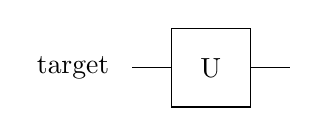
\begin{tikzpicture}[scale=.5] \node[draw=none] at (-3.5, 0) {target}; \draw (-2,0) -- (-1, 0); \draw (1, 0) -- (2, 0); \draw (-1,-1)--(-1,1)--(1,1)--(1,-1)--cycle; \node[draw=none] at (0, 0) {U}; \end{tikzpicture} } \]


\begin{DoxyParams}[1]{Parameters}
\mbox{\tt in,out}  & {\em multi\+Qubit} & object representing the set of all qubits \\
\hline
\mbox{\tt in}  & {\em target\+Qubit} & qubit to operate on \\
\hline
\mbox{\tt in}  & {\em alpha} & complex unitary parameter (row 1, column 1) \\
\hline
\mbox{\tt in}  & {\em beta} & complex unitary parameter (row 2, column 1) \\
\hline
\end{DoxyParams}

\begin{DoxyExceptions}{Exceptions}
{\em exit\+With\+Error} & if {\ttfamily target\+Qubit} is outside \mbox{[}0, {\ttfamily multi\+Qubit.\+num\+Qubits}), or if {\ttfamily alpha}, {\ttfamily beta} don\textquotesingle{}t satisfy $\vert${\ttfamily alpha$\vert$$^\wedge$2} + $\vert${\ttfamily beta$\vert$$^\wedge$2} = 1. \\
\hline
\end{DoxyExceptions}
\mbox{\Hypertarget{QuEST_8h_ab4812953bc457405b3aa05a4c2f64f4a}\label{QuEST_8h_ab4812953bc457405b3aa05a4c2f64f4a}} 
\index{Qu\+E\+S\+T.\+h@{Qu\+E\+S\+T.\+h}!controlled\+Compact\+Unitary@{controlled\+Compact\+Unitary}}
\index{controlled\+Compact\+Unitary@{controlled\+Compact\+Unitary}!Qu\+E\+S\+T.\+h@{Qu\+E\+S\+T.\+h}}
\paragraph{\texorpdfstring{controlled\+Compact\+Unitary()}{controlledCompactUnitary()}}
{\footnotesize\ttfamily void controlled\+Compact\+Unitary (\begin{DoxyParamCaption}\item[{\mbox{\hyperlink{structMultiQubit}{Multi\+Qubit}}}]{multi\+Qubit,  }\item[{const int}]{control\+Qubit,  }\item[{const int}]{target\+Qubit,  }\item[{\mbox{\hyperlink{structComplex}{Complex}}}]{alpha,  }\item[{\mbox{\hyperlink{structComplex}{Complex}}}]{beta }\end{DoxyParamCaption})}



Apply a controlled unitary (single control, single target) parameterised by two given complex scalars. 

Given valid complex numbers $\alpha$ and $\beta$, applies the two-\/qubit unitary \[ \begin{pmatrix} 1 \\ & 1 \\ & & \alpha & -\beta^* \\ & & \beta & \alpha^* \end{pmatrix} \] to the control and target qubits. Valid $\alpha$, $\beta$ satisfy $|\alpha|^2 + |\beta|^2 = 1$. The target unitary is general up to a global phase factor. ~\newline
 \[ \setlength{\fboxrule}{0.01pt} \fbox{ 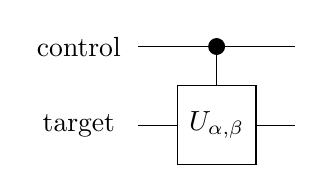
\begin{tikzpicture}[scale=.5] \node[draw=none] at (-3.5, 2) {control}; \node[draw=none] at (-3.5, 0) {target}; \draw (-2, 2) -- (2, 2); \draw[fill=black] (0, 2) circle (.2); \draw (0, 2) -- (0, 1); \draw (-2,0) -- (-1, 0); \draw (1, 0) -- (2, 0); \draw (-1,-1)--(-1,1)--(1,1)--(1,-1)--cycle; \node[draw=none] at (0, 0) {$U_{\alpha, \beta}$}; \end{tikzpicture} } \]


\begin{DoxyParams}[1]{Parameters}
\mbox{\tt in,out}  & {\em multi\+Qubit} & object representing the set of all qubits \\
\hline
\mbox{\tt in}  & {\em control\+Qubit} & apply the target unitary if this qubit has value 1 \\
\hline
\mbox{\tt in}  & {\em target\+Qubit} & qubit on which to apply the target unitary \\
\hline
\mbox{\tt in}  & {\em alpha} & complex unitary parameter (row 1, column 1) \\
\hline
\mbox{\tt in}  & {\em beta} & complex unitary parameter (row 2, column 1) \\
\hline
\end{DoxyParams}

\begin{DoxyExceptions}{Exceptions}
{\em exit\+With\+Error} & if either {\ttfamily control\+Qubit} or {\ttfamily target\+Qubit} are outside \mbox{[}0, {\ttfamily multi\+Qubit.\+num\+Qubits}) or are equal, or if {\ttfamily alpha}, {\ttfamily beta} don\textquotesingle{}t satisfy $\vert${\ttfamily alpha$\vert$$^\wedge$2} + $\vert${\ttfamily beta$\vert$$^\wedge$2} = 1. \\
\hline
\end{DoxyExceptions}
\mbox{\Hypertarget{QuEST_8h_a67576895bbc65463481a8ea24d9b1e22}\label{QuEST_8h_a67576895bbc65463481a8ea24d9b1e22}} 
\index{Qu\+E\+S\+T.\+h@{Qu\+E\+S\+T.\+h}!controlled\+Not@{controlled\+Not}}
\index{controlled\+Not@{controlled\+Not}!Qu\+E\+S\+T.\+h@{Qu\+E\+S\+T.\+h}}
\paragraph{\texorpdfstring{controlled\+Not()}{controlledNot()}}
{\footnotesize\ttfamily void controlled\+Not (\begin{DoxyParamCaption}\item[{\mbox{\hyperlink{structMultiQubit}{Multi\+Qubit}}}]{multi\+Qubit,  }\item[{const int}]{control\+Qubit,  }\item[{const int}]{target\+Qubit }\end{DoxyParamCaption})}



Apply the controlled not (single control, single target) gate, also known as the c-\/X, c-\/sigma-\/X, c-\/\+Pauli-\/X and c-\/bit-\/flip gate. 

This applies sigmaX to the target qubit if the control qubit has value 1. This effects the two-\/qubit unitary \[ \begin{pmatrix} 1 \\ & 1 \\\ & & & 1 \\ & & 1 \end{pmatrix} \] on the control and target qubits.

\[ \setlength{\fboxrule}{0.01pt} \fbox{ 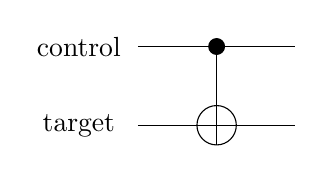
\begin{tikzpicture}[scale=.5] \node[draw=none] at (-3.5, 2) {control}; \node[draw=none] at (-3.5, 0) {target}; \draw (-2, 2) -- (2, 2); \draw[fill=black] (0, 2) circle (.2); \draw (0, 2) -- (0, -.5); \draw (-2,0) -- (2, 0); \draw (0, 0) circle (.5); \end{tikzpicture} } \] ~\newline
 
\begin{DoxyParams}[1]{Parameters}
\mbox{\tt in,out}  & {\em multi\+Qubit} & object representing the set of all qubits \\
\hline
\mbox{\tt in}  & {\em control\+Qubit} & nots the target if this qubit is 1 \\
\hline
\mbox{\tt in}  & {\em target\+Qubit} & qubit to not \\
\hline
\end{DoxyParams}

\begin{DoxyExceptions}{Exceptions}
{\em exit\+With\+Error} & if either {\ttfamily control\+Qubit} or {\ttfamily target\+Qubit} are outside \mbox{[}0, {\ttfamily multi\+Qubit.\+num\+Qubits}), or are equal. \\
\hline
\end{DoxyExceptions}
\mbox{\Hypertarget{QuEST_8h_a11a96159191cbf1b01a1080e7f045aac}\label{QuEST_8h_a11a96159191cbf1b01a1080e7f045aac}} 
\index{Qu\+E\+S\+T.\+h@{Qu\+E\+S\+T.\+h}!controlled\+Phase\+Gate@{controlled\+Phase\+Gate}}
\index{controlled\+Phase\+Gate@{controlled\+Phase\+Gate}!Qu\+E\+S\+T.\+h@{Qu\+E\+S\+T.\+h}}
\paragraph{\texorpdfstring{controlled\+Phase\+Gate()}{controlledPhaseGate()}}
{\footnotesize\ttfamily void controlled\+Phase\+Gate (\begin{DoxyParamCaption}\item[{\mbox{\hyperlink{structMultiQubit}{Multi\+Qubit}}}]{multi\+Qubit,  }\item[{const int}]{id\+Qubit1,  }\item[{const int}]{id\+Qubit2 }\end{DoxyParamCaption})}



Apply the (two-\/qubit) controlled phase gate, also known as the controlled sigmaZ gate. 

For each state, if both input qubits have value one, multiply the amplitude of that state by -\/1. This applies the two-\/qubit unitary\+: \[ \begin{pmatrix} 1 \\ & 1 \\\ & & 1 \\ & & & -1 \end{pmatrix} \]

\[ \setlength{\fboxrule}{0.01pt} \fbox{ 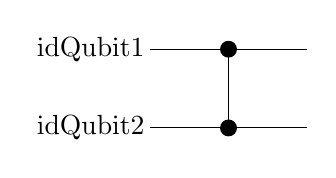
\begin{tikzpicture}[scale=.5] \node[draw=none] at (-3.5, 2) {idQubit1}; \node[draw=none] at (-3.5, 0) {idQubit2}; \draw (-2, 2) -- (2, 2); \draw[fill=black] (0, 2) circle (.2); \draw (0, 2) -- (0, 0); \draw (-2,0) -- (2, 0); \draw[fill=black] (0, 0) circle (.2); \end{tikzpicture} } \]


\begin{DoxyParams}[1]{Parameters}
\mbox{\tt in,out}  & {\em multi\+Qubit} & object representing the set of all qubits \\
\hline
\mbox{\tt in}  & {\em id\+Qubit1,id\+Qubit2} & qubits to operate upon \\
\hline
\end{DoxyParams}

\begin{DoxyExceptions}{Exceptions}
{\em exit\+With\+Error} & if {\ttfamily id\+Qubit1} or {\ttfamily id\+Qubit2} are outside \mbox{[}0, {\ttfamily multi\+Qubit.\+num\+Qubits}), or are equal \\
\hline
\end{DoxyExceptions}
\mbox{\Hypertarget{QuEST_8h_ad41f82b41149393a642391b67b3a287e}\label{QuEST_8h_ad41f82b41149393a642391b67b3a287e}} 
\index{Qu\+E\+S\+T.\+h@{Qu\+E\+S\+T.\+h}!controlled\+Rotate\+Around\+Axis@{controlled\+Rotate\+Around\+Axis}}
\index{controlled\+Rotate\+Around\+Axis@{controlled\+Rotate\+Around\+Axis}!Qu\+E\+S\+T.\+h@{Qu\+E\+S\+T.\+h}}
\paragraph{\texorpdfstring{controlled\+Rotate\+Around\+Axis()}{controlledRotateAroundAxis()}}
{\footnotesize\ttfamily void controlled\+Rotate\+Around\+Axis (\begin{DoxyParamCaption}\item[{\mbox{\hyperlink{structMultiQubit}{Multi\+Qubit}}}]{multi\+Qubit,  }\item[{const int}]{control\+Qubit,  }\item[{const int}]{target\+Qubit,  }\item[{\mbox{\hyperlink{QuEST__precision_8h_a4b654506f18b8bfd61ad2a29a7e38c25}{R\+E\+AL}}}]{angle,  }\item[{\mbox{\hyperlink{structVector}{Vector}}}]{axis }\end{DoxyParamCaption})}



Applies a controlled rotation by a given angle around a given vector on the Bloch-\/sphere. 

The vector must not be zero (else an error is thrown), but needn\textquotesingle{}t be unit magnitude.

For angle $\theta$ and axis vector $\vec{n}$, applies $R_{\hat{n}} = \exp \left(- i \frac{\theta}{2} \hat{n} \cdot \vec{\sigma} \right) $ to states where the target qubit is 1 ( $\vec{\sigma}$ is the vector of Pauli matrices).

\[ \setlength{\fboxrule}{0.01pt} \fbox{ 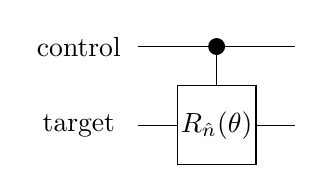
\begin{tikzpicture}[scale=.5] \node[draw=none] at (-3.5, 2) {control}; \node[draw=none] at (-3.5, 0) {target}; \draw (-2, 2) -- (2, 2); \draw[fill=black] (0, 2) circle (.2); \draw (0, 2) -- (0, 1); \draw (-2,0) -- (-1, 0); \draw (1, 0) -- (2, 0); \draw (-1,-1)--(-1,1)--(1,1)--(1,-1)--cycle; \node[draw=none] at (0, 0) {$R_{\hat{n}}(\theta)$}; \end{tikzpicture} } \]


\begin{DoxyParams}[1]{Parameters}
\mbox{\tt in,out}  & {\em multi\+Qubit} & object representing the set of all qubits \\
\hline
\mbox{\tt in}  & {\em control\+Qubit} & qubit with value 1 in the rotated states \\
\hline
\mbox{\tt in}  & {\em target\+Qubit} & qubit to rotate \\
\hline
\mbox{\tt in}  & {\em angle} & angle by which to rotate in radians \\
\hline
\mbox{\tt in}  & {\em axis} & vector around which to rotate (can be non-\/unit; will be normalised) \\
\hline
\end{DoxyParams}

\begin{DoxyExceptions}{Exceptions}
{\em exit\+With\+Error} & if either {\ttfamily control\+Qubit} or {\ttfamily target\+Qubit} are outside \mbox{[}0, {\ttfamily multi\+Qubit.\+num\+Qubits}) or are equal or if {\ttfamily axis} is the zero vector \\
\hline
\end{DoxyExceptions}
\mbox{\Hypertarget{QuEST_8h_ac6923ac57e67d9a21096e06f6a9012f6}\label{QuEST_8h_ac6923ac57e67d9a21096e06f6a9012f6}} 
\index{Qu\+E\+S\+T.\+h@{Qu\+E\+S\+T.\+h}!controlled\+RotateX@{controlled\+RotateX}}
\index{controlled\+RotateX@{controlled\+RotateX}!Qu\+E\+S\+T.\+h@{Qu\+E\+S\+T.\+h}}
\paragraph{\texorpdfstring{controlled\+Rotate\+X()}{controlledRotateX()}}
{\footnotesize\ttfamily void controlled\+RotateX (\begin{DoxyParamCaption}\item[{\mbox{\hyperlink{structMultiQubit}{Multi\+Qubit}}}]{multi\+Qubit,  }\item[{const int}]{control\+Qubit,  }\item[{const int}]{target\+Qubit,  }\item[{\mbox{\hyperlink{QuEST__precision_8h_a4b654506f18b8bfd61ad2a29a7e38c25}{R\+E\+AL}}}]{angle }\end{DoxyParamCaption})}



Applies a controlled rotation by a given angle around the X-\/axis of the Bloch-\/sphere. 

The target qubit is rotated in states where the control qubit has value 1.

\[ \setlength{\fboxrule}{0.01pt} \fbox{ 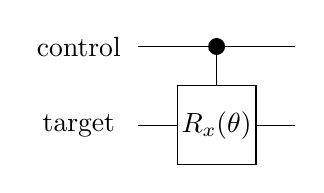
\begin{tikzpicture}[scale=.5] \node[draw=none] at (-3.5, 2) {control}; \node[draw=none] at (-3.5, 0) {target}; \draw (-2, 2) -- (2, 2); \draw[fill=black] (0, 2) circle (.2); \draw (0, 2) -- (0, 1); \draw (-2,0) -- (-1, 0); \draw (1, 0) -- (2, 0); \draw (-1,-1)--(-1,1)--(1,1)--(1,-1)--cycle; \node[draw=none] at (0, 0) {$R_x(\theta)$}; \end{tikzpicture} } \] ~\newline
 
\begin{DoxyParams}[1]{Parameters}
\mbox{\tt in,out}  & {\em multi\+Qubit} & object representing the set of all qubits \\
\hline
\mbox{\tt in}  & {\em control\+Qubit} & qubit which has value 1 in the rotated states \\
\hline
\mbox{\tt in}  & {\em tagret\+Qubit} & qubit to rotate \\
\hline
\mbox{\tt in}  & {\em angle} & angle by which to rotate the target qubit in radians \\
\hline
\end{DoxyParams}

\begin{DoxyExceptions}{Exceptions}
{\em exit\+With\+Error} & if either {\ttfamily control\+Qubit} or {\ttfamily target\+Qubit} are outside \mbox{[}0, {\ttfamily multi\+Qubit.\+num\+Qubits}) or are equal. \\
\hline
\end{DoxyExceptions}
\mbox{\Hypertarget{QuEST_8h_a71e90a2f7292116338c062934f9d1202}\label{QuEST_8h_a71e90a2f7292116338c062934f9d1202}} 
\index{Qu\+E\+S\+T.\+h@{Qu\+E\+S\+T.\+h}!controlled\+RotateY@{controlled\+RotateY}}
\index{controlled\+RotateY@{controlled\+RotateY}!Qu\+E\+S\+T.\+h@{Qu\+E\+S\+T.\+h}}
\paragraph{\texorpdfstring{controlled\+Rotate\+Y()}{controlledRotateY()}}
{\footnotesize\ttfamily void controlled\+RotateY (\begin{DoxyParamCaption}\item[{\mbox{\hyperlink{structMultiQubit}{Multi\+Qubit}}}]{multi\+Qubit,  }\item[{const int}]{control\+Qubit,  }\item[{const int}]{target\+Qubit,  }\item[{\mbox{\hyperlink{QuEST__precision_8h_a4b654506f18b8bfd61ad2a29a7e38c25}{R\+E\+AL}}}]{angle }\end{DoxyParamCaption})}



Applies a controlled rotation by a given angle around the Y-\/axis of the Bloch-\/sphere. 

The target qubit is rotated in states where the control qubit has value 1.

\[ \setlength{\fboxrule}{0.01pt} \fbox{ 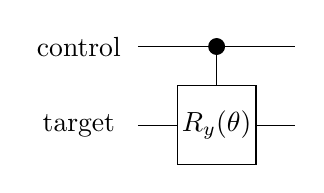
\begin{tikzpicture}[scale=.5] \node[draw=none] at (-3.5, 2) {control}; \node[draw=none] at (-3.5, 0) {target}; \draw (-2, 2) -- (2, 2); \draw[fill=black] (0, 2) circle (.2); \draw (0, 2) -- (0, 1); \draw (-2,0) -- (-1, 0); \draw (1, 0) -- (2, 0); \draw (-1,-1)--(-1,1)--(1,1)--(1,-1)--cycle; \node[draw=none] at (0, 0) {$R_y(\theta)$}; \end{tikzpicture} } \] ~\newline
 
\begin{DoxyParams}[1]{Parameters}
\mbox{\tt in,out}  & {\em multi\+Qubit} & object representing the set of all qubits \\
\hline
\mbox{\tt in}  & {\em control\+Qubit} & qubit which has value 1 in the rotated states \\
\hline
\mbox{\tt in}  & {\em tagret\+Qubit} & qubit to rotate \\
\hline
\mbox{\tt in}  & {\em angle} & angle by which to rotate the target qubit in radians \\
\hline
\end{DoxyParams}

\begin{DoxyExceptions}{Exceptions}
{\em exit\+With\+Error} & if either {\ttfamily control\+Qubit} or {\ttfamily target\+Qubit} are outside \mbox{[}0, {\ttfamily multi\+Qubit.\+num\+Qubits}) or are equal. \\
\hline
\end{DoxyExceptions}
\mbox{\Hypertarget{QuEST_8h_a668e5d2634b02e98bc73675ccb11d61c}\label{QuEST_8h_a668e5d2634b02e98bc73675ccb11d61c}} 
\index{Qu\+E\+S\+T.\+h@{Qu\+E\+S\+T.\+h}!controlled\+RotateZ@{controlled\+RotateZ}}
\index{controlled\+RotateZ@{controlled\+RotateZ}!Qu\+E\+S\+T.\+h@{Qu\+E\+S\+T.\+h}}
\paragraph{\texorpdfstring{controlled\+Rotate\+Z()}{controlledRotateZ()}}
{\footnotesize\ttfamily void controlled\+RotateZ (\begin{DoxyParamCaption}\item[{\mbox{\hyperlink{structMultiQubit}{Multi\+Qubit}}}]{multi\+Qubit,  }\item[{const int}]{control\+Qubit,  }\item[{const int}]{target\+Qubit,  }\item[{\mbox{\hyperlink{QuEST__precision_8h_a4b654506f18b8bfd61ad2a29a7e38c25}{R\+E\+AL}}}]{angle }\end{DoxyParamCaption})}



Applies a controlled rotation by a given angle around the Z-\/axis of the Bloch-\/sphere. 

The target qubit is rotated in states where the control qubit has value 1.

\[ \setlength{\fboxrule}{0.01pt} \fbox{ 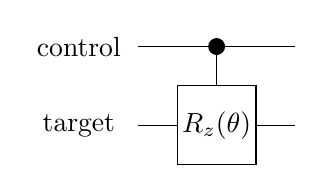
\begin{tikzpicture}[scale=.5] \node[draw=none] at (-3.5, 2) {control}; \node[draw=none] at (-3.5, 0) {target}; \draw (-2, 2) -- (2, 2); \draw[fill=black] (0, 2) circle (.2); \draw (0, 2) -- (0, 1); \draw (-2,0) -- (-1, 0); \draw (1, 0) -- (2, 0); \draw (-1,-1)--(-1,1)--(1,1)--(1,-1)--cycle; \node[draw=none] at (0, 0) {$R_z(\theta)$}; \end{tikzpicture} } \] ~\newline
 
\begin{DoxyParams}[1]{Parameters}
\mbox{\tt in,out}  & {\em multi\+Qubit} & object representing the set of all qubits \\
\hline
\mbox{\tt in}  & {\em control\+Qubit} & qubit which has value 1 in the rotated states \\
\hline
\mbox{\tt in}  & {\em tagret\+Qubit} & qubit to rotate \\
\hline
\mbox{\tt in}  & {\em angle} & angle by which to rotate the target qubit in radians \\
\hline
\end{DoxyParams}

\begin{DoxyExceptions}{Exceptions}
{\em exit\+With\+Error} & if either {\ttfamily control\+Qubit} or {\ttfamily target\+Qubit} are outside \mbox{[}0, {\ttfamily multi\+Qubit.\+num\+Qubits}) or are equal. \\
\hline
\end{DoxyExceptions}
\mbox{\Hypertarget{QuEST_8h_a8a701526263392599aa21d0d0f05d9d8}\label{QuEST_8h_a8a701526263392599aa21d0d0f05d9d8}} 
\index{Qu\+E\+S\+T.\+h@{Qu\+E\+S\+T.\+h}!controlled\+Unitary@{controlled\+Unitary}}
\index{controlled\+Unitary@{controlled\+Unitary}!Qu\+E\+S\+T.\+h@{Qu\+E\+S\+T.\+h}}
\paragraph{\texorpdfstring{controlled\+Unitary()}{controlledUnitary()}}
{\footnotesize\ttfamily void controlled\+Unitary (\begin{DoxyParamCaption}\item[{\mbox{\hyperlink{structMultiQubit}{Multi\+Qubit}}}]{multi\+Qubit,  }\item[{const int}]{control\+Qubit,  }\item[{const int}]{target\+Qubit,  }\item[{\mbox{\hyperlink{structComplexMatrix2}{Complex\+Matrix2}}}]{u }\end{DoxyParamCaption})}



Apply a general controlled unitary (single control, single target), which can include a global phase factor. 

The given unitary is applied to the target qubit if the control qubit has value 1, effecting the two-\/qubit unitary \[ \begin{pmatrix} 1 \\ & 1 \\ & & u_{00} & u_{01}\\ & & u_{10} & u_{11} \end{pmatrix} \] on the control and target qubits.

\[ \setlength{\fboxrule}{0.01pt} \fbox{ 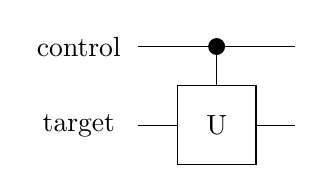
\begin{tikzpicture}[scale=.5] \node[draw=none] at (-3.5, 2) {control}; \node[draw=none] at (-3.5, 0) {target}; \draw (-2, 2) -- (2, 2); \draw[fill=black] (0, 2) circle (.2); \draw (0, 2) -- (0, 1); \draw (-2,0) -- (-1, 0); \draw (1, 0) -- (2, 0); \draw (-1,-1)--(-1,1)--(1,1)--(1,-1)--cycle; \node[draw=none] at (0, 0) {U}; \end{tikzpicture} } \]


\begin{DoxyParams}[1]{Parameters}
\mbox{\tt in,out}  & {\em multi\+Qubit} & object representing the set of all qubits \\
\hline
\mbox{\tt in}  & {\em control\+Qubit} & apply unitary if this qubit is 1 \\
\hline
\mbox{\tt in}  & {\em target\+Qubit} & qubit to operate on \\
\hline
\mbox{\tt in}  & {\em u} & single-\/qubit unitary matrix to apply \\
\hline
\end{DoxyParams}

\begin{DoxyExceptions}{Exceptions}
{\em exit\+With\+Error} & if either {\ttfamily control\+Qubit} or {\ttfamily target\+Qubit} are outside \mbox{[}0, {\ttfamily multi\+Qubit.\+num\+Qubits}) or are equal, or if {\ttfamily u} is not unitary. \\
\hline
\end{DoxyExceptions}
\mbox{\Hypertarget{QuEST_8h_a9c02591bc64c2918503afa231d90d83f}\label{QuEST_8h_a9c02591bc64c2918503afa231d90d83f}} 
\index{Qu\+E\+S\+T.\+h@{Qu\+E\+S\+T.\+h}!create\+Multi\+Qubit@{create\+Multi\+Qubit}}
\index{create\+Multi\+Qubit@{create\+Multi\+Qubit}!Qu\+E\+S\+T.\+h@{Qu\+E\+S\+T.\+h}}
\paragraph{\texorpdfstring{create\+Multi\+Qubit()}{createMultiQubit()}}
{\footnotesize\ttfamily void create\+Multi\+Qubit (\begin{DoxyParamCaption}\item[{\mbox{\hyperlink{structMultiQubit}{Multi\+Qubit}} $\ast$}]{multi\+Qubit,  }\item[{int}]{num\+Qubits,  }\item[{\mbox{\hyperlink{structQuESTEnv}{Qu\+E\+S\+T\+Env}}}]{env }\end{DoxyParamCaption})}



Create a \mbox{\hyperlink{structMultiQubit}{Multi\+Qubit}} object representing a set of qubits. 

Allocate space for state vector of probability amplitudes, including space for temporary values to be copied from one other chunk if running the distributed version. Define properties related to the size of the set of qubits. init\+State\+Zero should be called after this to initialise the qubits to the zero state.


\begin{DoxyParams}[1]{Parameters}
\mbox{\tt in,out}  & {\em multi\+Qubit} & a pointer to an object representing the set of qubits \\
\hline
\mbox{\tt in}  & {\em num\+Qubits} & number of qubits in the system \\
\hline
\mbox{\tt in}  & {\em env} & object representing the execution environment (local, multinode etc) \\
\hline
\end{DoxyParams}

\begin{DoxyExceptions}{Exceptions}
{\em exit\+With\+Error} & if {\ttfamily num\+Qubits} $<$= 0 \\
\hline
\end{DoxyExceptions}
\mbox{\Hypertarget{QuEST_8h_ae5d6acc322314d7a3d8a2eccf00d3b19}\label{QuEST_8h_ae5d6acc322314d7a3d8a2eccf00d3b19}} 
\index{Qu\+E\+S\+T.\+h@{Qu\+E\+S\+T.\+h}!destroy\+Multi\+Qubit@{destroy\+Multi\+Qubit}}
\index{destroy\+Multi\+Qubit@{destroy\+Multi\+Qubit}!Qu\+E\+S\+T.\+h@{Qu\+E\+S\+T.\+h}}
\paragraph{\texorpdfstring{destroy\+Multi\+Qubit()}{destroyMultiQubit()}}
{\footnotesize\ttfamily void destroy\+Multi\+Qubit (\begin{DoxyParamCaption}\item[{\mbox{\hyperlink{structMultiQubit}{Multi\+Qubit}}}]{multi\+Qubit,  }\item[{\mbox{\hyperlink{structQuESTEnv}{Qu\+E\+S\+T\+Env}}}]{env }\end{DoxyParamCaption})}



Deallocate a \mbox{\hyperlink{structMultiQubit}{Multi\+Qubit}} object representing a set of qubits. 

Free memory allocated to state vector of probability amplitudes, including temporary vector for values copied from another chunk if running the distributed version.


\begin{DoxyParams}[1]{Parameters}
\mbox{\tt in,out}  & {\em multi\+Qubit} & object to be deallocated \\
\hline
\mbox{\tt in}  & {\em env} & object representing the execution environment (local, multinode etc) \\
\hline
\end{DoxyParams}
\mbox{\Hypertarget{QuEST_8h_ad315c941a51bc053d39ebfa2040fd32e}\label{QuEST_8h_ad315c941a51bc053d39ebfa2040fd32e}} 
\index{Qu\+E\+S\+T.\+h@{Qu\+E\+S\+T.\+h}!find\+Probability\+Of\+Outcome@{find\+Probability\+Of\+Outcome}}
\index{find\+Probability\+Of\+Outcome@{find\+Probability\+Of\+Outcome}!Qu\+E\+S\+T.\+h@{Qu\+E\+S\+T.\+h}}
\paragraph{\texorpdfstring{find\+Probability\+Of\+Outcome()}{findProbabilityOfOutcome()}}
{\footnotesize\ttfamily \mbox{\hyperlink{QuEST__precision_8h_a4b654506f18b8bfd61ad2a29a7e38c25}{R\+E\+AL}} find\+Probability\+Of\+Outcome (\begin{DoxyParamCaption}\item[{\mbox{\hyperlink{structMultiQubit}{Multi\+Qubit}}}]{multi\+Qubit,  }\item[{const int}]{measure\+Qubit,  }\item[{int}]{outcome }\end{DoxyParamCaption})}



Gives the probability of a specified qubit being measured in the given outcome (0 or 1). 

This performs no actual measurement and does not change the state of the qubits.


\begin{DoxyParams}[1]{Parameters}
\mbox{\tt in}  & {\em multi\+Qubit} & object representing the set of all qubits \\
\hline
\mbox{\tt in}  & {\em measure\+Qubit} & qubit to study \\
\hline
\mbox{\tt in}  & {\em outcome} & for which to find the probability of the qubit being measured in \\
\hline
\end{DoxyParams}
\begin{DoxyReturn}{Returns}
probability of qubit measure\+Qubit being measured in the given outcome 
\end{DoxyReturn}

\begin{DoxyExceptions}{Exceptions}
{\em exit\+With\+Error} & if {\ttfamily measure\+Qubit} is outside \mbox{[}0, {\ttfamily multi\+Qubit.\+num\+Qubits}), or if {\ttfamily outcome} is not in \{0, 1\}. \\
\hline
\end{DoxyExceptions}
\mbox{\Hypertarget{QuEST_8h_a8f10aabf9f607f19093aee54630caa21}\label{QuEST_8h_a8f10aabf9f607f19093aee54630caa21}} 
\index{Qu\+E\+S\+T.\+h@{Qu\+E\+S\+T.\+h}!get\+Environment\+String@{get\+Environment\+String}}
\index{get\+Environment\+String@{get\+Environment\+String}!Qu\+E\+S\+T.\+h@{Qu\+E\+S\+T.\+h}}
\paragraph{\texorpdfstring{get\+Environment\+String()}{getEnvironmentString()}}
{\footnotesize\ttfamily void get\+Environment\+String (\begin{DoxyParamCaption}\item[{\mbox{\hyperlink{structQuESTEnv}{Qu\+E\+S\+T\+Env}}}]{env,  }\item[{\mbox{\hyperlink{structMultiQubit}{Multi\+Qubit}}}]{multi\+Qubit,  }\item[{char}]{str\mbox{[}200\mbox{]} }\end{DoxyParamCaption})}

\mbox{\Hypertarget{QuEST_8h_a3615f76fd5f57008d9b74bbd10533dd0}\label{QuEST_8h_a3615f76fd5f57008d9b74bbd10533dd0}} 
\index{Qu\+E\+S\+T.\+h@{Qu\+E\+S\+T.\+h}!get\+Imag\+Amp\+El@{get\+Imag\+Amp\+El}}
\index{get\+Imag\+Amp\+El@{get\+Imag\+Amp\+El}!Qu\+E\+S\+T.\+h@{Qu\+E\+S\+T.\+h}}
\paragraph{\texorpdfstring{get\+Imag\+Amp\+El()}{getImagAmpEl()}}
{\footnotesize\ttfamily \mbox{\hyperlink{QuEST__precision_8h_a4b654506f18b8bfd61ad2a29a7e38c25}{R\+E\+AL}} get\+Imag\+Amp\+El (\begin{DoxyParamCaption}\item[{\mbox{\hyperlink{structMultiQubit}{Multi\+Qubit}}}]{multi\+Qubit,  }\item[{long long int}]{index }\end{DoxyParamCaption})}



Get the imaginary component of the complex probability amplitude at an index in the state vector. 

For debugging purposes.


\begin{DoxyParams}[1]{Parameters}
\mbox{\tt in}  & {\em multi\+Qubit} & object representing a set of qubits \\
\hline
\mbox{\tt in}  & {\em index} & index in state vector of probability amplitudes \\
\hline
\end{DoxyParams}
\begin{DoxyReturn}{Returns}
imaginary component at that index 
\end{DoxyReturn}

\begin{DoxyExceptions}{Exceptions}
{\em exit\+With\+Error} & if {\ttfamily index} is outside \mbox{[}0, $2^{N}$) where $N = $ {\ttfamily multi\+Qubit.\+num\+Qubits} \\
\hline
\end{DoxyExceptions}
\mbox{\Hypertarget{QuEST_8h_ac61ecf4fd9ab2ac8453c4eb5b0d34089}\label{QuEST_8h_ac61ecf4fd9ab2ac8453c4eb5b0d34089}} 
\index{Qu\+E\+S\+T.\+h@{Qu\+E\+S\+T.\+h}!get\+Num\+Amps@{get\+Num\+Amps}}
\index{get\+Num\+Amps@{get\+Num\+Amps}!Qu\+E\+S\+T.\+h@{Qu\+E\+S\+T.\+h}}
\paragraph{\texorpdfstring{get\+Num\+Amps()}{getNumAmps()}}
{\footnotesize\ttfamily int get\+Num\+Amps (\begin{DoxyParamCaption}\item[{\mbox{\hyperlink{structMultiQubit}{Multi\+Qubit}}}]{multi\+Qubit }\end{DoxyParamCaption})}



Get the number of probability amplitudes in a multi\+Qubit object, given by 2$^\wedge$num\+Qubits. 

\mbox{\Hypertarget{QuEST_8h_a00e13dc88021b61a29fac9f3ab9ee850}\label{QuEST_8h_a00e13dc88021b61a29fac9f3ab9ee850}} 
\index{Qu\+E\+S\+T.\+h@{Qu\+E\+S\+T.\+h}!get\+Num\+Qubits@{get\+Num\+Qubits}}
\index{get\+Num\+Qubits@{get\+Num\+Qubits}!Qu\+E\+S\+T.\+h@{Qu\+E\+S\+T.\+h}}
\paragraph{\texorpdfstring{get\+Num\+Qubits()}{getNumQubits()}}
{\footnotesize\ttfamily int get\+Num\+Qubits (\begin{DoxyParamCaption}\item[{\mbox{\hyperlink{structMultiQubit}{Multi\+Qubit}}}]{multi\+Qubit }\end{DoxyParamCaption})}



Get the number of qubits in a multi\+Qubit object. 

\mbox{\Hypertarget{QuEST_8h_a799b10447d6dbdaf960a4d3eedd22014}\label{QuEST_8h_a799b10447d6dbdaf960a4d3eedd22014}} 
\index{Qu\+E\+S\+T.\+h@{Qu\+E\+S\+T.\+h}!get\+Prob\+El@{get\+Prob\+El}}
\index{get\+Prob\+El@{get\+Prob\+El}!Qu\+E\+S\+T.\+h@{Qu\+E\+S\+T.\+h}}
\paragraph{\texorpdfstring{get\+Prob\+El()}{getProbEl()}}
{\footnotesize\ttfamily \mbox{\hyperlink{QuEST__precision_8h_a4b654506f18b8bfd61ad2a29a7e38c25}{R\+E\+AL}} get\+Prob\+El (\begin{DoxyParamCaption}\item[{\mbox{\hyperlink{structMultiQubit}{Multi\+Qubit}}}]{multi\+Qubit,  }\item[{long long int}]{index }\end{DoxyParamCaption})}



Get the probability of the state at an index in the full state vector. 


\begin{DoxyParams}[1]{Parameters}
\mbox{\tt in}  & {\em multi\+Qubit} & object representing a set of qubits \\
\hline
\mbox{\tt in}  & {\em index} & index in state vector of probability amplitudes \\
\hline
\end{DoxyParams}
\begin{DoxyReturn}{Returns}
real\+El$\ast$real\+El + imag\+El$\ast$imag\+El 
\end{DoxyReturn}

\begin{DoxyExceptions}{Exceptions}
{\em exit\+With\+Error} & if {\ttfamily index} is outside \mbox{[}0, $2^{N}$) where $N = $ {\ttfamily multi\+Qubit.\+num\+Qubits} \\
\hline
\end{DoxyExceptions}
\mbox{\Hypertarget{QuEST_8h_a317b786f577fa6bc136ea7f0ee7330a7}\label{QuEST_8h_a317b786f577fa6bc136ea7f0ee7330a7}} 
\index{Qu\+E\+S\+T.\+h@{Qu\+E\+S\+T.\+h}!get\+Real\+Amp\+El@{get\+Real\+Amp\+El}}
\index{get\+Real\+Amp\+El@{get\+Real\+Amp\+El}!Qu\+E\+S\+T.\+h@{Qu\+E\+S\+T.\+h}}
\paragraph{\texorpdfstring{get\+Real\+Amp\+El()}{getRealAmpEl()}}
{\footnotesize\ttfamily \mbox{\hyperlink{QuEST__precision_8h_a4b654506f18b8bfd61ad2a29a7e38c25}{R\+E\+AL}} get\+Real\+Amp\+El (\begin{DoxyParamCaption}\item[{\mbox{\hyperlink{structMultiQubit}{Multi\+Qubit}}}]{multi\+Qubit,  }\item[{long long int}]{index }\end{DoxyParamCaption})}



Get the real component of the complex probability amplitude at an index in the state vector. 

For debugging purposes.


\begin{DoxyParams}[1]{Parameters}
\mbox{\tt in}  & {\em multi\+Qubit} & object representing a set of qubits \\
\hline
\mbox{\tt in}  & {\em index} & index in state vector of probability amplitudes \\
\hline
\end{DoxyParams}
\begin{DoxyReturn}{Returns}
real component at that index 
\end{DoxyReturn}

\begin{DoxyExceptions}{Exceptions}
{\em exit\+With\+Error} & if {\ttfamily index} is outside \mbox{[}0, $2^{N}$) where $N = $ {\ttfamily multi\+Qubit.\+num\+Qubits} \\
\hline
\end{DoxyExceptions}
\mbox{\Hypertarget{QuEST_8h_aa09b5dd93de6df1384b8f2c0041749ab}\label{QuEST_8h_aa09b5dd93de6df1384b8f2c0041749ab}} 
\index{Qu\+E\+S\+T.\+h@{Qu\+E\+S\+T.\+h}!hadamard@{hadamard}}
\index{hadamard@{hadamard}!Qu\+E\+S\+T.\+h@{Qu\+E\+S\+T.\+h}}
\paragraph{\texorpdfstring{hadamard()}{hadamard()}}
{\footnotesize\ttfamily void hadamard (\begin{DoxyParamCaption}\item[{\mbox{\hyperlink{structMultiQubit}{Multi\+Qubit}}}]{multi\+Qubit,  }\item[{const int}]{target\+Qubit }\end{DoxyParamCaption})}



Apply the single-\/qubit Hadamard gate. 

This takes $|0\rangle$ to $|+\rangle$ and $|1\rangle$ to $|-\rangle$, and is equivalent to a rotation of $\pi$ around the x-\/axis then $\pi/2$ about the y-\/axis on the Bloch-\/sphere. I.\+e. \[ \frac{1}{\sqrt{2}} \begin{pmatrix} 1 & 1 \\ 1 & -1 \end{pmatrix} \] ~\newline
 \[ \setlength{\fboxrule}{0.01pt} \fbox{ 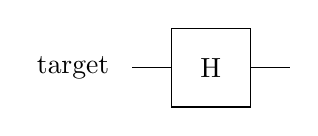
\begin{tikzpicture}[scale=.5] \node[draw=none] at (-3.5, 0) {target}; \draw (-2,0) -- (-1, 0); \draw (1, 0) -- (2, 0); \draw (-1,-1)--(-1,1)--(1,1)--(1,-1)--cycle; \node[draw=none] at (0, 0) {H}; \end{tikzpicture} } \] ~\newline
 
\begin{DoxyParams}[1]{Parameters}
\mbox{\tt in,out}  & {\em multi\+Qubit} & object representing the set of all qubits \\
\hline
\mbox{\tt in}  & {\em target\+Qubit} & qubit to operate on \\
\hline
\end{DoxyParams}

\begin{DoxyExceptions}{Exceptions}
{\em exit\+With\+Error} & if {\ttfamily target\+Qubit} is outside \mbox{[}0, {\ttfamily multi\+Qubit.\+num\+Qubits}). \\
\hline
\end{DoxyExceptions}
\mbox{\Hypertarget{QuEST_8h_aea34d45aaea9e64ad3f7786bfb412d0c}\label{QuEST_8h_aea34d45aaea9e64ad3f7786bfb412d0c}} 
\index{Qu\+E\+S\+T.\+h@{Qu\+E\+S\+T.\+h}!init\+Classical\+State@{init\+Classical\+State}}
\index{init\+Classical\+State@{init\+Classical\+State}!Qu\+E\+S\+T.\+h@{Qu\+E\+S\+T.\+h}}
\paragraph{\texorpdfstring{init\+Classical\+State()}{initClassicalState()}}
{\footnotesize\ttfamily void init\+Classical\+State (\begin{DoxyParamCaption}\item[{\mbox{\hyperlink{structMultiQubit}{Multi\+Qubit}} $\ast$}]{multi\+Qubit,  }\item[{long long int}]{state\+Ind }\end{DoxyParamCaption})}



Initialise a set of $ N $ qubits to the classical state with index {\ttfamily state\+Ind}. 

Note $ | 00 \dots 00 \rangle $ has {\ttfamily state\+Ind} 0, $ | 00 \dots 01 \rangle $ has {\ttfamily state\+Ind} 1, $ | 11 \dots 11 \rangle $ has {\ttfamily state\+Ind} $ 2^N - 1 $, etc. Subsequent calls to get\+Prob\+El will yield 0 for all indices except {\ttfamily state\+Ind}.


\begin{DoxyParams}[1]{Parameters}
\mbox{\tt in,out}  & {\em multi\+Qubit} & a pointer to the object representing the set of qubits to be initialised \\
\hline
\mbox{\tt in}  & {\em state\+Ind} & the index (0 to the number of amplitudes, exclusive) of the state to give probability 1 \\
\hline
\end{DoxyParams}
\mbox{\Hypertarget{QuEST_8h_ad84a3ce68d1ca02b4e3f741ea45b6054}\label{QuEST_8h_ad84a3ce68d1ca02b4e3f741ea45b6054}} 
\index{Qu\+E\+S\+T.\+h@{Qu\+E\+S\+T.\+h}!init\+Qu\+E\+S\+T\+Env@{init\+Qu\+E\+S\+T\+Env}}
\index{init\+Qu\+E\+S\+T\+Env@{init\+Qu\+E\+S\+T\+Env}!Qu\+E\+S\+T.\+h@{Qu\+E\+S\+T.\+h}}
\paragraph{\texorpdfstring{init\+Qu\+E\+S\+T\+Env()}{initQuESTEnv()}}
{\footnotesize\ttfamily void init\+Qu\+E\+S\+T\+Env (\begin{DoxyParamCaption}\item[{\mbox{\hyperlink{structQuESTEnv}{Qu\+E\+S\+T\+Env}} $\ast$}]{env }\end{DoxyParamCaption})}



Initialize the Qu\+E\+ST environment. 

If something needs to be done to set up the execution environment, such as initializing M\+PI when running in distributed mode, it is handled here


\begin{DoxyParams}[1]{Parameters}
\mbox{\tt in,out}  & {\em env} & object representing the execution environment. A single instance is used for each program \\
\hline
\end{DoxyParams}
\mbox{\Hypertarget{QuEST_8h_a43bcb279fc9717fbd06a19cdef48b9d8}\label{QuEST_8h_a43bcb279fc9717fbd06a19cdef48b9d8}} 
\index{Qu\+E\+S\+T.\+h@{Qu\+E\+S\+T.\+h}!init\+State\+Plus@{init\+State\+Plus}}
\index{init\+State\+Plus@{init\+State\+Plus}!Qu\+E\+S\+T.\+h@{Qu\+E\+S\+T.\+h}}
\paragraph{\texorpdfstring{init\+State\+Plus()}{initStatePlus()}}
{\footnotesize\ttfamily void init\+State\+Plus (\begin{DoxyParamCaption}\item[{\mbox{\hyperlink{structMultiQubit}{Multi\+Qubit}} $\ast$}]{multi\+Qubit }\end{DoxyParamCaption})}



Initialise a set of $ N $ qubits to the plus state $ {| + \rangle}^{\otimes N} = \frac{1}{\sqrt{2^N}} (| 0 \rangle + | 1 \rangle)^{\otimes N} $. 

This is the product state of $N$ qubits where every classical state is uniformly populated with real coefficient $\frac{1}{\sqrt{2^N}}$. This is equivalent to applying a Hadamard to every qubit in the zero state\+: $ \hat{H}^{\otimes N} {|0\rangle}^{\otimes N} $


\begin{DoxyParams}[1]{Parameters}
\mbox{\tt in,out}  & {\em multi\+Qubit} & a pointer to the object representing the set of qubits to be initialised \\
\hline
\end{DoxyParams}
\mbox{\Hypertarget{QuEST_8h_acb5b2eff794339090004d29f02a70d9a}\label{QuEST_8h_acb5b2eff794339090004d29f02a70d9a}} 
\index{Qu\+E\+S\+T.\+h@{Qu\+E\+S\+T.\+h}!init\+State\+Zero@{init\+State\+Zero}}
\index{init\+State\+Zero@{init\+State\+Zero}!Qu\+E\+S\+T.\+h@{Qu\+E\+S\+T.\+h}}
\paragraph{\texorpdfstring{init\+State\+Zero()}{initStateZero()}}
{\footnotesize\ttfamily void init\+State\+Zero (\begin{DoxyParamCaption}\item[{\mbox{\hyperlink{structMultiQubit}{Multi\+Qubit}} $\ast$}]{multi\+Qubit }\end{DoxyParamCaption})}



Initialise a set of $ N $ qubits to the classical zero state $ {| 0 \rangle}^{\otimes N} $. 


\begin{DoxyParams}[1]{Parameters}
\mbox{\tt in,out}  & {\em multi\+Qubit} & a pointer to the object representing the set of all qubits to initialise \\
\hline
\end{DoxyParams}
\mbox{\Hypertarget{QuEST_8h_ad5774247d836267175c664cd0e451bcb}\label{QuEST_8h_ad5774247d836267175c664cd0e451bcb}} 
\index{Qu\+E\+S\+T.\+h@{Qu\+E\+S\+T.\+h}!measure@{measure}}
\index{measure@{measure}!Qu\+E\+S\+T.\+h@{Qu\+E\+S\+T.\+h}}
\paragraph{\texorpdfstring{measure()}{measure()}}
{\footnotesize\ttfamily int measure (\begin{DoxyParamCaption}\item[{\mbox{\hyperlink{structMultiQubit}{Multi\+Qubit}}}]{multi\+Qubit,  }\item[{int}]{measure\+Qubit }\end{DoxyParamCaption})}



Measures a single qubit, collapsing it randomly to 0 or 1. 

Outcome probabilities are weighted by the state vector, which is irreversibly changed after collapse to be consistent with the outcome.


\begin{DoxyParams}[1]{Parameters}
\mbox{\tt in,out}  & {\em multi\+Qubit} & object representing the set of all qubits \\
\hline
\mbox{\tt in}  & {\em measure\+Qubit} & qubit to measure \\
\hline
\end{DoxyParams}
\begin{DoxyReturn}{Returns}
the measurement outcome, 0 or 1 
\end{DoxyReturn}

\begin{DoxyExceptions}{Exceptions}
{\em exit\+With\+Error} & if {\ttfamily measure\+Qubit} is outside \mbox{[}0, {\ttfamily multi\+Qubit.\+num\+Qubits}) \\
\hline
\end{DoxyExceptions}
\mbox{\Hypertarget{QuEST_8h_a2ac46e470c750bf93c754e06c64b0a7a}\label{QuEST_8h_a2ac46e470c750bf93c754e06c64b0a7a}} 
\index{Qu\+E\+S\+T.\+h@{Qu\+E\+S\+T.\+h}!measure\+With\+Stats@{measure\+With\+Stats}}
\index{measure\+With\+Stats@{measure\+With\+Stats}!Qu\+E\+S\+T.\+h@{Qu\+E\+S\+T.\+h}}
\paragraph{\texorpdfstring{measure\+With\+Stats()}{measureWithStats()}}
{\footnotesize\ttfamily int measure\+With\+Stats (\begin{DoxyParamCaption}\item[{\mbox{\hyperlink{structMultiQubit}{Multi\+Qubit}}}]{multi\+Qubit,  }\item[{int}]{measure\+Qubit,  }\item[{\mbox{\hyperlink{QuEST__precision_8h_a4b654506f18b8bfd61ad2a29a7e38c25}{R\+E\+AL}} $\ast$}]{state\+Prob }\end{DoxyParamCaption})}



Measures a single qubit, collapsing it randomly to 0 or 1, and additionally gives the probability of that outcome. 

Outcome probabilities are weighted by the state vector, which is irreversibly changed after collapse to be consistent with the outcome.


\begin{DoxyParams}[1]{Parameters}
\mbox{\tt in,out}  & {\em multi\+Qubit} & object representing the set of all qubits \\
\hline
\mbox{\tt in}  & {\em measure\+Qubit} & qubit to measure \\
\hline
\mbox{\tt out}  & {\em state\+Prob} & a pointer to a R\+E\+AL which is set to the probability of the occurred outcome \\
\hline
\end{DoxyParams}
\begin{DoxyReturn}{Returns}
the measurement outcome, 0 or 1 
\end{DoxyReturn}

\begin{DoxyExceptions}{Exceptions}
{\em exit\+With\+Error} & if {\ttfamily measure\+Qubit} is outside \mbox{[}0, {\ttfamily multi\+Qubit.\+num\+Qubits}) \\
\hline
\end{DoxyExceptions}
\mbox{\Hypertarget{QuEST_8h_afc1835c6b43b6e59ce7df7b13f274fc7}\label{QuEST_8h_afc1835c6b43b6e59ce7df7b13f274fc7}} 
\index{Qu\+E\+S\+T.\+h@{Qu\+E\+S\+T.\+h}!multi\+Controlled\+Phase\+Gate@{multi\+Controlled\+Phase\+Gate}}
\index{multi\+Controlled\+Phase\+Gate@{multi\+Controlled\+Phase\+Gate}!Qu\+E\+S\+T.\+h@{Qu\+E\+S\+T.\+h}}
\paragraph{\texorpdfstring{multi\+Controlled\+Phase\+Gate()}{multiControlledPhaseGate()}}
{\footnotesize\ttfamily void multi\+Controlled\+Phase\+Gate (\begin{DoxyParamCaption}\item[{\mbox{\hyperlink{structMultiQubit}{Multi\+Qubit}}}]{multi\+Qubit,  }\item[{int $\ast$}]{control\+Qubits,  }\item[{int}]{num\+Control\+Qubits }\end{DoxyParamCaption})}



Apply the multiple-\/qubit controlled phase gate, also known as the multiple-\/qubit controlled sigmaZ gate. 

For each state, if all control qubits have value one, multiply the amplitude of that state by -\/1. This applies the many-\/qubit unitary\+: \[ \begin{pmatrix} 1 \\ & 1 \\\ & & \ddots \\ & & & 1 \\ & & & & -1 \end{pmatrix} \] on the control qubits.

\[ \setlength{\fboxrule}{0.01pt} \fbox{ \begin{tikzpicture}[scale=.5] \node[draw=none] at (-3.5, 2) {controls}; \node[draw=none] at (0, 6) {$\vdots$}; \draw (0, 5) -- (0, 4); \draw (-2, 4) -- (2, 4); \draw[fill=black] (0, 4) circle (.2); \draw (0, 4) -- (0, 2); \draw (-2, 2) -- (2, 2); \draw[fill=black] (0, 2) circle (.2); \draw (0, 2) -- (0, 0); \draw (-2,0) -- (2, 0); \draw[fill=black] (0, 0) circle (.2); \end{tikzpicture} } \]


\begin{DoxyParams}[1]{Parameters}
\mbox{\tt in,out}  & {\em multi\+Qubit} & object representing the set of all qubits \\
\hline
\mbox{\tt in}  & {\em control\+Qubits} & array of input qubits \\
\hline
\mbox{\tt in}  & {\em num\+Control\+Qubits} & number of input qubits \\
\hline
\end{DoxyParams}

\begin{DoxyExceptions}{Exceptions}
{\em exit\+With\+Error} & if {\ttfamily num\+Control\+Qubits} is outside \mbox{[}1, {\ttfamily multi\+Qubit.\+num\+Qubits}) \\
\hline
\end{DoxyExceptions}
\mbox{\Hypertarget{QuEST_8h_ae395a79690283ed81106afadd7a8cd8a}\label{QuEST_8h_ae395a79690283ed81106afadd7a8cd8a}} 
\index{Qu\+E\+S\+T.\+h@{Qu\+E\+S\+T.\+h}!multi\+Controlled\+Unitary@{multi\+Controlled\+Unitary}}
\index{multi\+Controlled\+Unitary@{multi\+Controlled\+Unitary}!Qu\+E\+S\+T.\+h@{Qu\+E\+S\+T.\+h}}
\paragraph{\texorpdfstring{multi\+Controlled\+Unitary()}{multiControlledUnitary()}}
{\footnotesize\ttfamily void multi\+Controlled\+Unitary (\begin{DoxyParamCaption}\item[{\mbox{\hyperlink{structMultiQubit}{Multi\+Qubit}}}]{multi\+Qubit,  }\item[{int $\ast$}]{control\+Qubits,  }\item[{const int}]{num\+Control\+Qubits,  }\item[{const int}]{target\+Qubit,  }\item[{\mbox{\hyperlink{structComplexMatrix2}{Complex\+Matrix2}}}]{u }\end{DoxyParamCaption})}



Apply a general multiple-\/control single-\/target unitary, which can include a global phase factor. 

Any number of control qubits can be specified, and if all have value 1, the given unitary is applied to the target qubit. This effects the many-\/qubit unitary \[ \begin{pmatrix} 1 \\ & 1 \\\ & & \ddots \\ & & & u_{00} & u_{01}\\ & & & u_{10} & u_{11} \end{pmatrix} \] on the control and target qubits. The given 2x2 Complex\+Matrix must be unitary, otherwise an error is thrown.

\[ \setlength{\fboxrule}{0.01pt} \fbox{ 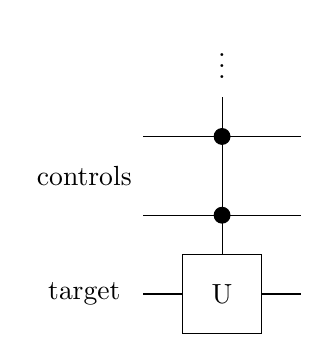
\begin{tikzpicture}[scale=.5] \node[draw=none] at (-3.5, 3) {controls}; \node[draw=none] at (-3.5, 0) {target}; \node[draw=none] at (0, 6) {$\vdots$}; \draw (0, 5) -- (0, 4); \draw (-2, 4) -- (2, 4); \draw[fill=black] (0, 4) circle (.2); \draw (0, 4) -- (0, 2); \draw (-2, 2) -- (2, 2); \draw[fill=black] (0, 2) circle (.2); \draw (0, 2) -- (0, 1); \draw (-2,0) -- (-1, 0); \draw (1, 0) -- (2, 0); \draw (-1,-1)--(-1,1)--(1,1)--(1,-1)--cycle; \node[draw=none] at (0, 0) {U}; \end{tikzpicture} } \]


\begin{DoxyParams}[1]{Parameters}
\mbox{\tt in,out}  & {\em multi\+Qubit} & object representing the set of all qubits \\
\hline
\mbox{\tt in}  & {\em control\+Qubits} & applies unitary if all qubits in this array equal 1 \\
\hline
\mbox{\tt in}  & {\em num\+Control\+Qubits} & number of control qubits \\
\hline
\mbox{\tt in}  & {\em target\+Qubit} & qubit to operate on \\
\hline
\mbox{\tt in}  & {\em u} & single-\/qubit unitary matrix to apply \\
\hline
\end{DoxyParams}

\begin{DoxyExceptions}{Exceptions}
{\em exit\+With\+Error} & if {\ttfamily num\+Control\+Qubits} is outside \mbox{[}1, {\ttfamily multi\+Qubit.\+num\+Qubits}\mbox{]}), or if any qubit index ({\ttfamily target\+Qubit} or one in {\ttfamily control\+Qubits}) is outside \mbox{[}0, {\ttfamily multi\+Qubit.\+num\+Qubits}\mbox{]}), or if {\ttfamily control\+Qubits} contains {\ttfamily target\+Qubit}, or if {\ttfamily u} is not unitary. \\
\hline
\end{DoxyExceptions}
\mbox{\Hypertarget{QuEST_8h_aedb5ef39da69e7895d714980dc621261}\label{QuEST_8h_aedb5ef39da69e7895d714980dc621261}} 
\index{Qu\+E\+S\+T.\+h@{Qu\+E\+S\+T.\+h}!Qu\+E\+S\+T\+Seed\+Random@{Qu\+E\+S\+T\+Seed\+Random}}
\index{Qu\+E\+S\+T\+Seed\+Random@{Qu\+E\+S\+T\+Seed\+Random}!Qu\+E\+S\+T.\+h@{Qu\+E\+S\+T.\+h}}
\paragraph{\texorpdfstring{Qu\+E\+S\+T\+Seed\+Random()}{QuESTSeedRandom()}}
{\footnotesize\ttfamily void Qu\+E\+S\+T\+Seed\+Random (\begin{DoxyParamCaption}\item[{unsigned long int $\ast$}]{seed\+Array,  }\item[{int}]{num\+Seeds }\end{DoxyParamCaption})}



Seed the Mersenne Twister used for random number generation in the Qu\+E\+ST environment with a user defined seed. 

This function uses the mt19937 init\+\_\+by\+\_\+array function with num\+Seeds keys supplied by the user. Subsequent calls to mt19937 genrand functions will use this seeding. For a multi process code, the same seed is given to all process, therefore this seeding is only appropriate to use for functions such as measure where all processes require the same random value.


\begin{DoxyParams}[1]{Parameters}
\mbox{\tt in}  & {\em seed\+Array} & Array of integers to use as seed. This allows the MT to be initialised with more than a 32-\/bit integer if required \\
\hline
\mbox{\tt in}  & {\em num\+Seeds} & Length of seed\+Array\\
\hline
\end{DoxyParams}
For more information about the MT, see \href{http://www.math.sci.hiroshima-u.ac.jp/~m-mat/MT/MT2002/emt19937ar.html}{\tt http\+://www.\+math.\+sci.\+hiroshima-\/u.\+ac.\+jp/$\sim$m-\/mat/\+M\+T/\+M\+T2002/emt19937ar.\+html} \mbox{\Hypertarget{QuEST_8h_ac49f548ee27ae484695f9add1273adb4}\label{QuEST_8h_ac49f548ee27ae484695f9add1273adb4}} 
\index{Qu\+E\+S\+T.\+h@{Qu\+E\+S\+T.\+h}!Qu\+E\+S\+T\+Seed\+Random\+Default@{Qu\+E\+S\+T\+Seed\+Random\+Default}}
\index{Qu\+E\+S\+T\+Seed\+Random\+Default@{Qu\+E\+S\+T\+Seed\+Random\+Default}!Qu\+E\+S\+T.\+h@{Qu\+E\+S\+T.\+h}}
\paragraph{\texorpdfstring{Qu\+E\+S\+T\+Seed\+Random\+Default()}{QuESTSeedRandomDefault()}}
{\footnotesize\ttfamily void Qu\+E\+S\+T\+Seed\+Random\+Default (\begin{DoxyParamCaption}\item[{void}]{ }\end{DoxyParamCaption})}



Seed the Mersenne Twister used for random number generation in the Qu\+E\+ST environment with an example defualt seed. 

This default seeding function uses the mt19937 init\+\_\+by\+\_\+array function with three keys -- time, pid and hostname. Subsequent calls to mt19937 genrand functions will use this seeding. For a multi process code, the same seed is given to all process, therefore this seeding is only appropriate to use for functions such as measure where all processes require the same random value.

For more information about the MT, see \href{http://www.math.sci.hiroshima-u.ac.jp/~m-mat/MT/MT2002/emt19937ar.html}{\tt http\+://www.\+math.\+sci.\+hiroshima-\/u.\+ac.\+jp/$\sim$m-\/mat/\+M\+T/\+M\+T2002/emt19937ar.\+html} \mbox{\Hypertarget{QuEST_8h_aa5e77e0e64f3a4a3d3f5cc7382bffcd9}\label{QuEST_8h_aa5e77e0e64f3a4a3d3f5cc7382bffcd9}} 
\index{Qu\+E\+S\+T.\+h@{Qu\+E\+S\+T.\+h}!report\+Multi\+Qubit\+Params@{report\+Multi\+Qubit\+Params}}
\index{report\+Multi\+Qubit\+Params@{report\+Multi\+Qubit\+Params}!Qu\+E\+S\+T.\+h@{Qu\+E\+S\+T.\+h}}
\paragraph{\texorpdfstring{report\+Multi\+Qubit\+Params()}{reportMultiQubitParams()}}
{\footnotesize\ttfamily void report\+Multi\+Qubit\+Params (\begin{DoxyParamCaption}\item[{\mbox{\hyperlink{structMultiQubit}{Multi\+Qubit}}}]{multi\+Qubit }\end{DoxyParamCaption})}



Report metainformation about a set of qubits\+: number of qubits, number of probability amplitudes. 


\begin{DoxyParams}[1]{Parameters}
\mbox{\tt in,out}  & {\em multi\+Qubit} & object representing the set of qubits \\
\hline
\mbox{\tt in}  & {\em env} & object representing the execution environment (local, multinode etc) \\
\hline
\end{DoxyParams}
\mbox{\Hypertarget{QuEST_8h_af8a14ae79c3fb2c0b5f6255cc37bebf9}\label{QuEST_8h_af8a14ae79c3fb2c0b5f6255cc37bebf9}} 
\index{Qu\+E\+S\+T.\+h@{Qu\+E\+S\+T.\+h}!report\+Qu\+E\+S\+T\+Env@{report\+Qu\+E\+S\+T\+Env}}
\index{report\+Qu\+E\+S\+T\+Env@{report\+Qu\+E\+S\+T\+Env}!Qu\+E\+S\+T.\+h@{Qu\+E\+S\+T.\+h}}
\paragraph{\texorpdfstring{report\+Qu\+E\+S\+T\+Env()}{reportQuESTEnv()}}
{\footnotesize\ttfamily void report\+Qu\+E\+S\+T\+Env (\begin{DoxyParamCaption}\item[{\mbox{\hyperlink{structQuESTEnv}{Qu\+E\+S\+T\+Env}}}]{env }\end{DoxyParamCaption})}



Report information about the Qu\+E\+ST environment. 


\begin{DoxyParams}[1]{Parameters}
\mbox{\tt in}  & {\em env} & object representing the execution environment. A single instance is used for each program \\
\hline
\end{DoxyParams}
\mbox{\Hypertarget{QuEST_8h_a96f4de9ce7fefc7680a44d601fc3d894}\label{QuEST_8h_a96f4de9ce7fefc7680a44d601fc3d894}} 
\index{Qu\+E\+S\+T.\+h@{Qu\+E\+S\+T.\+h}!report\+State@{report\+State}}
\index{report\+State@{report\+State}!Qu\+E\+S\+T.\+h@{Qu\+E\+S\+T.\+h}}
\paragraph{\texorpdfstring{report\+State()}{reportState()}}
{\footnotesize\ttfamily void report\+State (\begin{DoxyParamCaption}\item[{\mbox{\hyperlink{structMultiQubit}{Multi\+Qubit}}}]{multi\+Qubit }\end{DoxyParamCaption})}



Print the current state vector of probability amplitudes for a set of qubits to file. 

File format\+: \begin{DoxyVerb}real, imag
realComponent1, imagComponent1
realComponent2, imagComponent2
...
realComponentN, imagComponentN
\end{DoxyVerb}


File naming convention\+:

For each node that the program runs on, a file \textquotesingle{}state\+\_\+rank\+\_\+\mbox{[}node\+\_\+rank\mbox{]}.csv\textquotesingle{} is generated. If there is more than one node, ranks after the first do not include the header \begin{DoxyVerb}real, imag
\end{DoxyVerb}
 so that files are easier to combine.


\begin{DoxyParams}[1]{Parameters}
\mbox{\tt in,out}  & {\em multi\+Qubit} & object representing the set of qubits \\
\hline
\end{DoxyParams}
\mbox{\Hypertarget{QuEST_8h_a842d6884e063a5865a2232cba56b65ac}\label{QuEST_8h_a842d6884e063a5865a2232cba56b65ac}} 
\index{Qu\+E\+S\+T.\+h@{Qu\+E\+S\+T.\+h}!report\+State\+To\+Screen@{report\+State\+To\+Screen}}
\index{report\+State\+To\+Screen@{report\+State\+To\+Screen}!Qu\+E\+S\+T.\+h@{Qu\+E\+S\+T.\+h}}
\paragraph{\texorpdfstring{report\+State\+To\+Screen()}{reportStateToScreen()}}
{\footnotesize\ttfamily void report\+State\+To\+Screen (\begin{DoxyParamCaption}\item[{\mbox{\hyperlink{structMultiQubit}{Multi\+Qubit}}}]{multi\+Qubit,  }\item[{\mbox{\hyperlink{structQuESTEnv}{Qu\+E\+S\+T\+Env}}}]{env,  }\item[{int}]{report\+Rank }\end{DoxyParamCaption})}



Print the current state vector of probability amplitudes for a set of qubits to standard out. 

For debugging purposes. Each rank should print output serially. Only print output for systems $<$= 5 qubits \mbox{\Hypertarget{QuEST_8h_a8810423457803005fecd415f4299f40d}\label{QuEST_8h_a8810423457803005fecd415f4299f40d}} 
\index{Qu\+E\+S\+T.\+h@{Qu\+E\+S\+T.\+h}!rotate\+Around\+Axis@{rotate\+Around\+Axis}}
\index{rotate\+Around\+Axis@{rotate\+Around\+Axis}!Qu\+E\+S\+T.\+h@{Qu\+E\+S\+T.\+h}}
\paragraph{\texorpdfstring{rotate\+Around\+Axis()}{rotateAroundAxis()}}
{\footnotesize\ttfamily void rotate\+Around\+Axis (\begin{DoxyParamCaption}\item[{\mbox{\hyperlink{structMultiQubit}{Multi\+Qubit}}}]{multi\+Qubit,  }\item[{const int}]{rot\+Qubit,  }\item[{\mbox{\hyperlink{QuEST__precision_8h_a4b654506f18b8bfd61ad2a29a7e38c25}{R\+E\+AL}}}]{angle,  }\item[{\mbox{\hyperlink{structVector}{Vector}}}]{axis }\end{DoxyParamCaption})}



Rotate a single qubit by a given angle around a given vector on the Bloch-\/sphere. 

The vector must not be zero (else an error is thrown), but needn\textquotesingle{}t be unit magnitude.

For angle $\theta$ and axis vector $\vec{n}$, applies $R_{\hat{n}} = \exp \left(- i \frac{\theta}{2} \hat{n} \cdot \vec{\sigma} \right) $ where $\vec{\sigma}$ is the vector of Pauli matrices.


\begin{DoxyParams}[1]{Parameters}
\mbox{\tt in,out}  & {\em multi\+Qubit} & object representing the set of all qubits \\
\hline
\mbox{\tt in}  & {\em rot\+Qubit} & qubit to rotate \\
\hline
\mbox{\tt in}  & {\em angle} & angle by which to rotate in radians \\
\hline
\mbox{\tt in}  & {\em axis} & vector around which to rotate (can be non-\/unit; will be normalised) \\
\hline
\end{DoxyParams}

\begin{DoxyExceptions}{Exceptions}
{\em exit\+With\+Error} & if {\ttfamily rot\+Qubit} is outside \mbox{[}0, {\ttfamily multi\+Qubit.\+num\+Qubits}), or if {\ttfamily axis} is the zero vector \\
\hline
\end{DoxyExceptions}
\mbox{\Hypertarget{QuEST_8h_a6cc7fa705a2f2e6b486b49c5589d5df5}\label{QuEST_8h_a6cc7fa705a2f2e6b486b49c5589d5df5}} 
\index{Qu\+E\+S\+T.\+h@{Qu\+E\+S\+T.\+h}!rotateX@{rotateX}}
\index{rotateX@{rotateX}!Qu\+E\+S\+T.\+h@{Qu\+E\+S\+T.\+h}}
\paragraph{\texorpdfstring{rotate\+X()}{rotateX()}}
{\footnotesize\ttfamily void rotateX (\begin{DoxyParamCaption}\item[{\mbox{\hyperlink{structMultiQubit}{Multi\+Qubit}}}]{multi\+Qubit,  }\item[{const int}]{rot\+Qubit,  }\item[{\mbox{\hyperlink{QuEST__precision_8h_a4b654506f18b8bfd61ad2a29a7e38c25}{R\+E\+AL}}}]{angle }\end{DoxyParamCaption})}



Rotate a single qubit by a given angle around the X-\/axis of the Bloch-\/sphere. 

For angle $\theta$, applies \[ \begin{pmatrix} \cos\theta/2 & -i \sin \theta/2\\ -i \sin \theta/2 & \cos \theta/2 \end{pmatrix} \]

\[ \setlength{\fboxrule}{0.01pt} \fbox{ 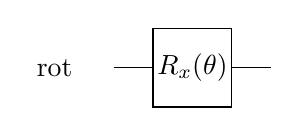
\begin{tikzpicture}[scale=.5] \node[draw=none] at (-3.5, 0) {rot}; \draw (-2,0) -- (-1, 0); \draw (1, 0) -- (2, 0); \draw (-1,-1)--(-1,1)--(1,1)--(1,-1)--cycle; \node[draw=none] at (0, 0) {$R_x(\theta)$}; \end{tikzpicture} } \]


\begin{DoxyParams}[1]{Parameters}
\mbox{\tt in,out}  & {\em multi\+Qubit} & object representing the set of all qubits \\
\hline
\mbox{\tt in}  & {\em rot\+Qubit} & qubit to rotate \\
\hline
\mbox{\tt in}  & {\em angle} & angle by which to rotate in radians \\
\hline
\end{DoxyParams}

\begin{DoxyExceptions}{Exceptions}
{\em exit\+With\+Error} & if {\ttfamily rot\+Qubit} is outside \mbox{[}0, {\ttfamily multi\+Qubit.\+num\+Qubits}). \\
\hline
\end{DoxyExceptions}
\mbox{\Hypertarget{QuEST_8h_ace0d3592d38a990e81a434c4e9681500}\label{QuEST_8h_ace0d3592d38a990e81a434c4e9681500}} 
\index{Qu\+E\+S\+T.\+h@{Qu\+E\+S\+T.\+h}!rotateY@{rotateY}}
\index{rotateY@{rotateY}!Qu\+E\+S\+T.\+h@{Qu\+E\+S\+T.\+h}}
\paragraph{\texorpdfstring{rotate\+Y()}{rotateY()}}
{\footnotesize\ttfamily void rotateY (\begin{DoxyParamCaption}\item[{\mbox{\hyperlink{structMultiQubit}{Multi\+Qubit}}}]{multi\+Qubit,  }\item[{const int}]{rot\+Qubit,  }\item[{\mbox{\hyperlink{QuEST__precision_8h_a4b654506f18b8bfd61ad2a29a7e38c25}{R\+E\+AL}}}]{angle }\end{DoxyParamCaption})}



Rotate a single qubit by a given angle around the Y-\/axis of the Bloch-\/sphere. 

For angle $\theta$, applies \[ \begin{pmatrix} \cos\theta/2 & - \sin \theta/2\\ \sin \theta/2 & \cos \theta/2 \end{pmatrix} \] ~\newline
 \[ \setlength{\fboxrule}{0.01pt} \fbox{ 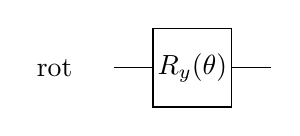
\begin{tikzpicture}[scale=.5] \node[draw=none] at (-3.5, 0) {rot}; \draw (-2,0) -- (-1, 0); \draw (1, 0) -- (2, 0); \draw (-1,-1)--(-1,1)--(1,1)--(1,-1)--cycle; \node[draw=none] at (0, 0) {$R_y(\theta)$}; \end{tikzpicture} } \]


\begin{DoxyParams}[1]{Parameters}
\mbox{\tt in,out}  & {\em multi\+Qubit} & object representing the set of all qubits \\
\hline
\mbox{\tt in}  & {\em rot\+Qubit} & qubit to rotate \\
\hline
\mbox{\tt in}  & {\em angle} & angle by which to rotate in radians \\
\hline
\end{DoxyParams}

\begin{DoxyExceptions}{Exceptions}
{\em exit\+With\+Error} & if {\ttfamily rot\+Qubit} is outside \mbox{[}0, {\ttfamily multi\+Qubit.\+num\+Qubits}). \\
\hline
\end{DoxyExceptions}
\mbox{\Hypertarget{QuEST_8h_abd621412ad30c1b034f4ce153c4afe10}\label{QuEST_8h_abd621412ad30c1b034f4ce153c4afe10}} 
\index{Qu\+E\+S\+T.\+h@{Qu\+E\+S\+T.\+h}!rotateZ@{rotateZ}}
\index{rotateZ@{rotateZ}!Qu\+E\+S\+T.\+h@{Qu\+E\+S\+T.\+h}}
\paragraph{\texorpdfstring{rotate\+Z()}{rotateZ()}}
{\footnotesize\ttfamily void rotateZ (\begin{DoxyParamCaption}\item[{\mbox{\hyperlink{structMultiQubit}{Multi\+Qubit}}}]{multi\+Qubit,  }\item[{const int}]{rot\+Qubit,  }\item[{\mbox{\hyperlink{QuEST__precision_8h_a4b654506f18b8bfd61ad2a29a7e38c25}{R\+E\+AL}}}]{angle }\end{DoxyParamCaption})}



Rotate a single qubit by a given angle around the Z-\/axis of the Bloch-\/sphere (also known as a phase shift gate). 

For angle $\theta$, applies \[ \begin{pmatrix} \exp(-i \theta/2) & 0 \\ 0 & \exp(i \theta/2) \end{pmatrix} \]

\[ \setlength{\fboxrule}{0.01pt} \fbox{ 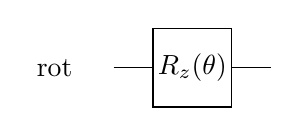
\begin{tikzpicture}[scale=.5] \node[draw=none] at (-3.5, 0) {rot}; \draw (-2,0) -- (-1, 0); \draw (1, 0) -- (2, 0); \draw (-1,-1)--(-1,1)--(1,1)--(1,-1)--cycle; \node[draw=none] at (0, 0) {$R_z(\theta)$}; \end{tikzpicture} } \]


\begin{DoxyParams}[1]{Parameters}
\mbox{\tt in,out}  & {\em multi\+Qubit} & object representing the set of all qubits \\
\hline
\mbox{\tt in}  & {\em rot\+Qubit} & qubit to rotate \\
\hline
\mbox{\tt in}  & {\em angle} & angle by which to rotate in radians \\
\hline
\end{DoxyParams}

\begin{DoxyExceptions}{Exceptions}
{\em exit\+With\+Error} & if {\ttfamily rot\+Qubit} is outside \mbox{[}0, {\ttfamily multi\+Qubit.\+num\+Qubits}). \\
\hline
\end{DoxyExceptions}
\mbox{\Hypertarget{QuEST_8h_adda6c47876a7676488ed0565a19eaa65}\label{QuEST_8h_adda6c47876a7676488ed0565a19eaa65}} 
\index{Qu\+E\+S\+T.\+h@{Qu\+E\+S\+T.\+h}!s\+Gate@{s\+Gate}}
\index{s\+Gate@{s\+Gate}!Qu\+E\+S\+T.\+h@{Qu\+E\+S\+T.\+h}}
\paragraph{\texorpdfstring{s\+Gate()}{sGate()}}
{\footnotesize\ttfamily void s\+Gate (\begin{DoxyParamCaption}\item[{\mbox{\hyperlink{structMultiQubit}{Multi\+Qubit}}}]{multi\+Qubit,  }\item[{const int}]{target\+Qubit }\end{DoxyParamCaption})}



Apply the single-\/qubit S gate. 

This is a rotation of $\pi/2$ around the Z-\/axis on the Bloch sphere, or the unitary\+: \[ \begin{pmatrix} 1 & 0 \\ 0 & i \end{pmatrix} \]

\[ \setlength{\fboxrule}{0.01pt} \fbox{ 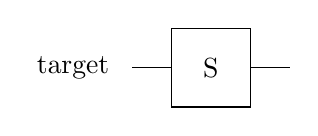
\begin{tikzpicture}[scale=.5] \node[draw=none] at (-3.5, 0) {target}; \draw (-2,0) -- (-1, 0); \draw (1, 0) -- (2, 0); \draw (-1,-1)--(-1,1)--(1,1)--(1,-1)--cycle; \node[draw=none] at (0, 0) {S}; \end{tikzpicture} } \]


\begin{DoxyParams}[1]{Parameters}
\mbox{\tt in,out}  & {\em multi\+Qubit} & object representing the set of all qubits \\
\hline
\mbox{\tt in}  & {\em target\+Qubit} & qubit to operate upon \\
\hline
\end{DoxyParams}

\begin{DoxyExceptions}{Exceptions}
{\em exit\+With\+Error} & if {\ttfamily target\+Qubit} is outside \mbox{[}0, {\ttfamily multi\+Qubit.\+num\+Qubits}) \\
\hline
\end{DoxyExceptions}
\mbox{\Hypertarget{QuEST_8h_a86e396e06b7d527cac20ba0108872423}\label{QuEST_8h_a86e396e06b7d527cac20ba0108872423}} 
\index{Qu\+E\+S\+T.\+h@{Qu\+E\+S\+T.\+h}!sigmaX@{sigmaX}}
\index{sigmaX@{sigmaX}!Qu\+E\+S\+T.\+h@{Qu\+E\+S\+T.\+h}}
\paragraph{\texorpdfstring{sigma\+X()}{sigmaX()}}
{\footnotesize\ttfamily void sigmaX (\begin{DoxyParamCaption}\item[{\mbox{\hyperlink{structMultiQubit}{Multi\+Qubit}}}]{multi\+Qubit,  }\item[{const int}]{target\+Qubit }\end{DoxyParamCaption})}



Apply the single-\/qubit sigma-\/X (also known as the X, Pauli-\/X, N\+OT or bit-\/flip) gate. 

This is a rotation of $\pi$ around the x-\/axis on the Bloch sphere. I.\+e. \[ \begin{pmatrix} 0 & 1 \\ 1 & 0 \end{pmatrix} \] ~\newline
 \[ \setlength{\fboxrule}{0.01pt} \fbox{ 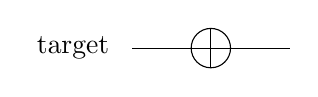
\begin{tikzpicture}[scale=.5] \node[draw=none] at (-3.5, 0) {target}; \draw (-2,0) -- (2, 0); \draw (0, 0) circle (.5); \draw (0, .5) -- (0, -.5); \end{tikzpicture} } \] ~\newline
 
\begin{DoxyParams}[1]{Parameters}
\mbox{\tt in,out}  & {\em multi\+Qubit} & object representing the set of all qubits \\
\hline
\mbox{\tt in}  & {\em target\+Qubit} & qubit to operate on \\
\hline
\end{DoxyParams}

\begin{DoxyExceptions}{Exceptions}
{\em exit\+With\+Error} & if {\ttfamily target\+Qubit} is outside \mbox{[}0, {\ttfamily multi\+Qubit.\+num\+Qubits}). \\
\hline
\end{DoxyExceptions}
\mbox{\Hypertarget{QuEST_8h_a1f54d70a42403f7e1c2e2c2007332f61}\label{QuEST_8h_a1f54d70a42403f7e1c2e2c2007332f61}} 
\index{Qu\+E\+S\+T.\+h@{Qu\+E\+S\+T.\+h}!sigmaY@{sigmaY}}
\index{sigmaY@{sigmaY}!Qu\+E\+S\+T.\+h@{Qu\+E\+S\+T.\+h}}
\paragraph{\texorpdfstring{sigma\+Y()}{sigmaY()}}
{\footnotesize\ttfamily void sigmaY (\begin{DoxyParamCaption}\item[{\mbox{\hyperlink{structMultiQubit}{Multi\+Qubit}}}]{multi\+Qubit,  }\item[{const int}]{target\+Qubit }\end{DoxyParamCaption})}



Apply the single-\/qubit sigma-\/Y (also known as the Y or Pauli-\/Y) gate. 

This is a rotation of $\pi$ around the Y-\/axis on the Bloch sphere. I.\+e. \[ \begin{pmatrix} 0 & -i \\ i & 0 \end{pmatrix} \] ~\newline
 \[ \setlength{\fboxrule}{0.01pt} \fbox{ 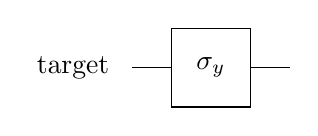
\begin{tikzpicture}[scale=.5] \node[draw=none] at (-3.5, 0) {target}; \draw (-2,0) -- (-1, 0); \draw (1, 0) -- (2, 0); \draw (-1,-1)--(-1,1)--(1,1)--(1,-1)--cycle; \node[draw=none] at (0, 0) {$\sigma_y$}; \end{tikzpicture} } \] ~\newline
 
\begin{DoxyParams}[1]{Parameters}
\mbox{\tt in,out}  & {\em multi\+Qubit} & object representing the set of all qubits \\
\hline
\mbox{\tt in}  & {\em target\+Qubit} & qubit to operate on \\
\hline
\end{DoxyParams}

\begin{DoxyExceptions}{Exceptions}
{\em exit\+With\+Error} & if {\ttfamily target\+Qubit} is outside \mbox{[}0, {\ttfamily multi\+Qubit.\+num\+Qubits}). \\
\hline
\end{DoxyExceptions}
\mbox{\Hypertarget{QuEST_8h_aebaab86326779de55d335cfea3efde8f}\label{QuEST_8h_aebaab86326779de55d335cfea3efde8f}} 
\index{Qu\+E\+S\+T.\+h@{Qu\+E\+S\+T.\+h}!sigmaZ@{sigmaZ}}
\index{sigmaZ@{sigmaZ}!Qu\+E\+S\+T.\+h@{Qu\+E\+S\+T.\+h}}
\paragraph{\texorpdfstring{sigma\+Z()}{sigmaZ()}}
{\footnotesize\ttfamily void sigmaZ (\begin{DoxyParamCaption}\item[{\mbox{\hyperlink{structMultiQubit}{Multi\+Qubit}}}]{multi\+Qubit,  }\item[{const int}]{target\+Qubit }\end{DoxyParamCaption})}



Apply the single-\/qubit sigma-\/Z (also known as the Z, Pauli-\/Z or phase-\/flip) gate. 

This is a rotation of $\pi$ around the Z-\/axis (a phase shift) on the Bloch sphere. I.\+e. \[ \begin{pmatrix} 1 & 0 \\ 0 & -1 \end{pmatrix} \] ~\newline
 \[ \setlength{\fboxrule}{0.01pt} \fbox{ 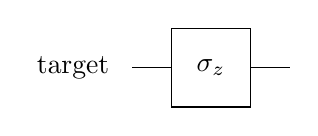
\begin{tikzpicture}[scale=.5] \node[draw=none] at (-3.5, 0) {target}; \draw (-2,0) -- (-1, 0); \draw (1, 0) -- (2, 0); \draw (-1,-1)--(-1,1)--(1,1)--(1,-1)--cycle; \node[draw=none] at (0, 0) {$\sigma_z$}; \end{tikzpicture} } \] ~\newline
 
\begin{DoxyParams}[1]{Parameters}
\mbox{\tt in,out}  & {\em multi\+Qubit} & object representing the set of all qubits \\
\hline
\mbox{\tt in}  & {\em target\+Qubit} & qubit to operate on \\
\hline
\end{DoxyParams}

\begin{DoxyExceptions}{Exceptions}
{\em exit\+With\+Error} & if {\ttfamily target\+Qubit} is outside \mbox{[}0, {\ttfamily multi\+Qubit.\+num\+Qubits}). \\
\hline
\end{DoxyExceptions}
\mbox{\Hypertarget{QuEST_8h_a8d31fe2d1ad4d01e2a1f5f6b8bc15b77}\label{QuEST_8h_a8d31fe2d1ad4d01e2a1f5f6b8bc15b77}} 
\index{Qu\+E\+S\+T.\+h@{Qu\+E\+S\+T.\+h}!sync\+Qu\+E\+S\+T\+Env@{sync\+Qu\+E\+S\+T\+Env}}
\index{sync\+Qu\+E\+S\+T\+Env@{sync\+Qu\+E\+S\+T\+Env}!Qu\+E\+S\+T.\+h@{Qu\+E\+S\+T.\+h}}
\paragraph{\texorpdfstring{sync\+Qu\+E\+S\+T\+Env()}{syncQuESTEnv()}}
{\footnotesize\ttfamily void sync\+Qu\+E\+S\+T\+Env (\begin{DoxyParamCaption}\item[{\mbox{\hyperlink{structQuESTEnv}{Qu\+E\+S\+T\+Env}}}]{env }\end{DoxyParamCaption})}



Guarantees that all code up to the given point has been executed on all nodes (if running in distributed mode) 


\begin{DoxyParams}[1]{Parameters}
\mbox{\tt in}  & {\em env} & object representing the execution environment. A single instance is used for each program \\
\hline
\end{DoxyParams}
\mbox{\Hypertarget{QuEST_8h_ac7e38d768a1bd79019f88cc1e6295092}\label{QuEST_8h_ac7e38d768a1bd79019f88cc1e6295092}} 
\index{Qu\+E\+S\+T.\+h@{Qu\+E\+S\+T.\+h}!sync\+Qu\+E\+S\+T\+Success@{sync\+Qu\+E\+S\+T\+Success}}
\index{sync\+Qu\+E\+S\+T\+Success@{sync\+Qu\+E\+S\+T\+Success}!Qu\+E\+S\+T.\+h@{Qu\+E\+S\+T.\+h}}
\paragraph{\texorpdfstring{sync\+Qu\+E\+S\+T\+Success()}{syncQuESTSuccess()}}
{\footnotesize\ttfamily int sync\+Qu\+E\+S\+T\+Success (\begin{DoxyParamCaption}\item[{int}]{success\+Code }\end{DoxyParamCaption})}



Performs a logical A\+ND on all success\+Codes held by all processes. 

If any one process has a zero success\+Code all processes will return a zero success code.


\begin{DoxyParams}[1]{Parameters}
\mbox{\tt in}  & {\em env} & object representing the execution environment. A single instance is used for each program \\
\hline
\mbox{\tt in}  & {\em success\+Code} & 1 if process task succeeded, 0 if process task failed \\
\hline
\end{DoxyParams}
\begin{DoxyReturn}{Returns}
1 if all processes succeeded, 0 if any one process failed 
\end{DoxyReturn}
\mbox{\Hypertarget{QuEST_8h_af764ea63a2e870098f4e1ce08562942e}\label{QuEST_8h_af764ea63a2e870098f4e1ce08562942e}} 
\index{Qu\+E\+S\+T.\+h@{Qu\+E\+S\+T.\+h}!t\+Gate@{t\+Gate}}
\index{t\+Gate@{t\+Gate}!Qu\+E\+S\+T.\+h@{Qu\+E\+S\+T.\+h}}
\paragraph{\texorpdfstring{t\+Gate()}{tGate()}}
{\footnotesize\ttfamily void t\+Gate (\begin{DoxyParamCaption}\item[{\mbox{\hyperlink{structMultiQubit}{Multi\+Qubit}}}]{multi\+Qubit,  }\item[{const int}]{target\+Qubit }\end{DoxyParamCaption})}



Apply the single-\/qubit T gate. 

This is a rotation of $\pi/4$ around the Z-\/axis on the Bloch sphere, or the unitary\+: \[ \begin{pmatrix} 1 & 0 \\ 0 & \exp\left(i \frac{\pi}{4}\right) \end{pmatrix} \]

\[ \setlength{\fboxrule}{0.01pt} \fbox{ 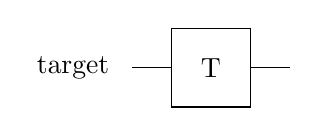
\begin{tikzpicture}[scale=.5] \node[draw=none] at (-3.5, 0) {target}; \draw (-2,0) -- (-1, 0); \draw (1, 0) -- (2, 0); \draw (-1,-1)--(-1,1)--(1,1)--(1,-1)--cycle; \node[draw=none] at (0, 0) {T}; \end{tikzpicture} } \]


\begin{DoxyParams}[1]{Parameters}
\mbox{\tt in,out}  & {\em multi\+Qubit} & object representing the set of all qubits \\
\hline
\mbox{\tt in}  & {\em target\+Qubit} & qubit to operate upon \\
\hline
\end{DoxyParams}

\begin{DoxyExceptions}{Exceptions}
{\em exit\+With\+Error} & if {\ttfamily target\+Qubit} is outside \mbox{[}0, {\ttfamily multi\+Qubit.\+num\+Qubits}) \\
\hline
\end{DoxyExceptions}
\mbox{\Hypertarget{QuEST_8h_a7a0877e33700f6bad48adb51b7b3fb67}\label{QuEST_8h_a7a0877e33700f6bad48adb51b7b3fb67}} 
\index{Qu\+E\+S\+T.\+h@{Qu\+E\+S\+T.\+h}!unitary@{unitary}}
\index{unitary@{unitary}!Qu\+E\+S\+T.\+h@{Qu\+E\+S\+T.\+h}}
\paragraph{\texorpdfstring{unitary()}{unitary()}}
{\footnotesize\ttfamily void unitary (\begin{DoxyParamCaption}\item[{\mbox{\hyperlink{structMultiQubit}{Multi\+Qubit}}}]{multi\+Qubit,  }\item[{const int}]{target\+Qubit,  }\item[{\mbox{\hyperlink{structComplexMatrix2}{Complex\+Matrix2}}}]{u }\end{DoxyParamCaption})}



Apply a general single-\/qubit unitary (including a global phase factor). 

The passed 2x2 Complex\+Matrix must be unitary, otherwise an error is thrown.

\[ \setlength{\fboxrule}{0.01pt} \fbox{ 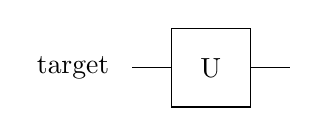
\begin{tikzpicture}[scale=.5] \node[draw=none] at (-3.5, 0) {target}; \draw (-2,0) -- (-1, 0); \draw (1, 0) -- (2, 0); \draw (-1,-1)--(-1,1)--(1,1)--(1,-1)--cycle; \node[draw=none] at (0, 0) {U}; \end{tikzpicture} } \]


\begin{DoxyParams}[1]{Parameters}
\mbox{\tt in,out}  & {\em multi\+Qubit} & object representing the set of all qubits \\
\hline
\mbox{\tt in}  & {\em target\+Qubit} & qubit to operate on \\
\hline
\mbox{\tt in}  & {\em u} & unitary matrix to apply \\
\hline
\end{DoxyParams}

\begin{DoxyExceptions}{Exceptions}
{\em exit\+With\+Error} & if {\ttfamily target\+Qubit} is outside \mbox{[}0, {\ttfamily multi\+Qubit.\+num\+Qubits}), or matrix {\ttfamily u} is not unitary. \\
\hline
\end{DoxyExceptions}

\hypertarget{QuEST__debug_8h}{}\subsection{Qu\+E\+S\+T\+\_\+debug.\+h File Reference}
\label{QuEST__debug_8h}\index{Qu\+E\+S\+T\+\_\+debug.\+h@{Qu\+E\+S\+T\+\_\+debug.\+h}}


Developer functions used for unit testing and debugging.  


{\ttfamily \#include \char`\"{}Qu\+E\+S\+T\+\_\+precision.\+h\char`\"{}}\newline
\subsubsection*{Functions}
\begin{DoxyCompactItemize}
\item 
void \mbox{\hyperlink{QuEST__debug_8h_a7169fd0442cbc3418f3fac4d13363ca2}{init\+State\+Of\+Single\+Qubit}} (\mbox{\hyperlink{structMultiQubit}{Multi\+Qubit}} $\ast$multi\+Qubit, int qubit\+Id, int outcome)
\begin{DoxyCompactList}\small\item\em Initialise the state vector of probability amplitudes such that one qubit is set to \textquotesingle{}outcome\textquotesingle{} and all other qubits are in an equal superposition of zero and one. \end{DoxyCompactList}\item 
void \mbox{\hyperlink{QuEST__debug_8h_a03b3577a891731d505bc4b879fcca9d3}{init\+State\+Debug}} (\mbox{\hyperlink{structMultiQubit}{Multi\+Qubit}} $\ast$multi\+Qubit)
\begin{DoxyCompactList}\small\item\em Initialise the state vector of probability amplitudes to an (unphysical) state with each component of each probability amplitude a unique floating point value. \end{DoxyCompactList}\item 
void \mbox{\hyperlink{QuEST__debug_8h_a433876ee9f3bcc54af346300f571fc3c}{initialize\+State\+From\+Single\+File}} (\mbox{\hyperlink{structMultiQubit}{Multi\+Qubit}} $\ast$multi\+Qubit, char filename\mbox{[}200\mbox{]}, \mbox{\hyperlink{structQuESTEnv}{Qu\+E\+S\+T\+Env}} env)
\item 
int \mbox{\hyperlink{QuEST__debug_8h_a793584932ae384c82e7e42db7d35d18d}{compare\+States}} (\mbox{\hyperlink{structMultiQubit}{Multi\+Qubit}} mq1, \mbox{\hyperlink{structMultiQubit}{Multi\+Qubit}} mq2, \mbox{\hyperlink{QuEST__precision_8h_a4b654506f18b8bfd61ad2a29a7e38c25}{R\+E\+AL}} precision)
\item 
void \mbox{\hyperlink{QuEST__debug_8h_a62da5b58d8ce84e6f4d24be1b872294e}{report\+Node\+List}} (\mbox{\hyperlink{structQuESTEnv}{Qu\+E\+S\+T\+Env}} env)
\begin{DoxyCompactList}\small\item\em Report a list of C\+PU hostnames and the rank that is running on each if running with M\+PI enabled and an error message otherwise. \end{DoxyCompactList}\end{DoxyCompactItemize}


\subsubsection{Detailed Description}
Developer functions used for unit testing and debugging. 

Not part of the public A\+PI. May contain functions that are incomplete or untested. 

\subsubsection{Function Documentation}
\mbox{\Hypertarget{QuEST__debug_8h_a793584932ae384c82e7e42db7d35d18d}\label{QuEST__debug_8h_a793584932ae384c82e7e42db7d35d18d}} 
\index{Qu\+E\+S\+T\+\_\+debug.\+h@{Qu\+E\+S\+T\+\_\+debug.\+h}!compare\+States@{compare\+States}}
\index{compare\+States@{compare\+States}!Qu\+E\+S\+T\+\_\+debug.\+h@{Qu\+E\+S\+T\+\_\+debug.\+h}}
\paragraph{\texorpdfstring{compare\+States()}{compareStates()}}
{\footnotesize\ttfamily int compare\+States (\begin{DoxyParamCaption}\item[{\mbox{\hyperlink{structMultiQubit}{Multi\+Qubit}}}]{mq1,  }\item[{\mbox{\hyperlink{structMultiQubit}{Multi\+Qubit}}}]{mq2,  }\item[{\mbox{\hyperlink{QuEST__precision_8h_a4b654506f18b8bfd61ad2a29a7e38c25}{R\+E\+AL}}}]{precision }\end{DoxyParamCaption})}



Definition at line 372 of file Qu\+E\+S\+T.\+c.



References Complex\+Array\+::imag, Multi\+Qubit\+::num\+Amps, Complex\+Array\+::real, R\+E\+AL, and Multi\+Qubit\+::state\+Vec.


\begin{DoxyCode}
372                                                                  \{
373     \mbox{\hyperlink{QuEST__precision_8h_a4b654506f18b8bfd61ad2a29a7e38c25}{REAL}} diff;
374     \textcolor{keywordtype}{int} chunkSize = mq1.\mbox{\hyperlink{structMultiQubit_ae16f47d8b725c914fb7f66b6498d79db}{numAmps}};
375     \textcolor{keywordflow}{for} (\textcolor{keywordtype}{int} i=0; i<chunkSize; i++)\{
376         diff = fabs(mq1.\mbox{\hyperlink{structMultiQubit_a45483190d6b01ef6b2f98f2bec9ab94f}{stateVec}}.\mbox{\hyperlink{structComplexArray_a4195cac6c784ea1b6271f1c7dba1548a}{real}}[i] - mq2.\mbox{\hyperlink{structMultiQubit_a45483190d6b01ef6b2f98f2bec9ab94f}{stateVec}}.\mbox{\hyperlink{structComplexArray_a4195cac6c784ea1b6271f1c7dba1548a}{real}}[i]);
377         \textcolor{keywordflow}{if} (diff>precision) \textcolor{keywordflow}{return} 0;
378         diff = fabs(mq1.\mbox{\hyperlink{structMultiQubit_a45483190d6b01ef6b2f98f2bec9ab94f}{stateVec}}.\mbox{\hyperlink{structComplexArray_a79dde47c7ae530c79cebfdf57b225968}{imag}}[i] - mq2.\mbox{\hyperlink{structMultiQubit_a45483190d6b01ef6b2f98f2bec9ab94f}{stateVec}}.\mbox{\hyperlink{structComplexArray_a79dde47c7ae530c79cebfdf57b225968}{imag}}[i]);
379         \textcolor{keywordflow}{if} (diff>precision) \textcolor{keywordflow}{return} 0;
380     \}
381     \textcolor{keywordflow}{return} 1;
382 \}
\end{DoxyCode}
\mbox{\Hypertarget{QuEST__debug_8h_a433876ee9f3bcc54af346300f571fc3c}\label{QuEST__debug_8h_a433876ee9f3bcc54af346300f571fc3c}} 
\index{Qu\+E\+S\+T\+\_\+debug.\+h@{Qu\+E\+S\+T\+\_\+debug.\+h}!initialize\+State\+From\+Single\+File@{initialize\+State\+From\+Single\+File}}
\index{initialize\+State\+From\+Single\+File@{initialize\+State\+From\+Single\+File}!Qu\+E\+S\+T\+\_\+debug.\+h@{Qu\+E\+S\+T\+\_\+debug.\+h}}
\paragraph{\texorpdfstring{initialize\+State\+From\+Single\+File()}{initializeStateFromSingleFile()}}
{\footnotesize\ttfamily void initialize\+State\+From\+Single\+File (\begin{DoxyParamCaption}\item[{\mbox{\hyperlink{structMultiQubit}{Multi\+Qubit}} $\ast$}]{multi\+Qubit,  }\item[{char}]{filename\mbox{[}200\mbox{]},  }\item[{\mbox{\hyperlink{structQuESTEnv}{Qu\+E\+S\+T\+Env}}}]{env }\end{DoxyParamCaption})}

fix -- format needs to work for single precision values 

Definition at line 336 of file Qu\+E\+S\+T.\+c.



References Multi\+Qubit\+::chunk\+Id, Complex\+Array\+::imag, Multi\+Qubit\+::num\+Amps, Multi\+Qubit\+::num\+Chunks, Qu\+E\+S\+T\+Assert(), Complex\+Array\+::real, R\+E\+AL, Multi\+Qubit\+::state\+Vec, and sync\+Qu\+E\+S\+T\+Env().


\begin{DoxyCode}
336                                                                                             \{
337     \textcolor{keywordtype}{long} \textcolor{keywordtype}{long} \textcolor{keywordtype}{int} chunkSize, stateVecSize;
338     \textcolor{keywordtype}{long} \textcolor{keywordtype}{long} \textcolor{keywordtype}{int} indexInChunk, totalIndex;
339 
340     chunkSize = multiQubit->\mbox{\hyperlink{structMultiQubit_ae16f47d8b725c914fb7f66b6498d79db}{numAmps}};
341     stateVecSize = chunkSize*multiQubit->\mbox{\hyperlink{structMultiQubit_acd43f2f57991709c9e94f73662c972b2}{numChunks}};
342 
343     \mbox{\hyperlink{QuEST__precision_8h_a4b654506f18b8bfd61ad2a29a7e38c25}{REAL}} *stateVecReal = multiQubit->\mbox{\hyperlink{structMultiQubit_a45483190d6b01ef6b2f98f2bec9ab94f}{stateVec}}.\mbox{\hyperlink{structComplexArray_a4195cac6c784ea1b6271f1c7dba1548a}{real}};
344     \mbox{\hyperlink{QuEST__precision_8h_a4b654506f18b8bfd61ad2a29a7e38c25}{REAL}} *stateVecImag = multiQubit->\mbox{\hyperlink{structMultiQubit_a45483190d6b01ef6b2f98f2bec9ab94f}{stateVec}}.\mbox{\hyperlink{structComplexArray_a79dde47c7ae530c79cebfdf57b225968}{imag}};
345 
346     FILE *fp;
347     \textcolor{keywordtype}{char} line[200];
348 
349     \textcolor{keywordflow}{for} (\textcolor{keywordtype}{int} rank=0; rank<(multiQubit->\mbox{\hyperlink{structMultiQubit_acd43f2f57991709c9e94f73662c972b2}{numChunks}}); rank++)\{
350         \textcolor{keywordflow}{if} (rank==multiQubit->\mbox{\hyperlink{structMultiQubit_ab10c88249fa3825d6227ceec01d37e37}{chunkId}})\{
351             fp = fopen(filename, \textcolor{stringliteral}{"r"});
352             \mbox{\hyperlink{QuEST__env__local_8c_a3587b9d533e633ccf1abf9ad2ce45d8d}{QuESTAssert}}(fp!=NULL, 11, \_\_func\_\_);
353             indexInChunk = 0; totalIndex = 0;
354             \textcolor{keywordflow}{while} (fgets(line, \textcolor{keyword}{sizeof}(\textcolor{keywordtype}{char})*200, fp) != NULL && totalIndex<stateVecSize)\{
355                 \textcolor{keywordflow}{if} (line[0]!=\textcolor{charliteral}{'#'})\{
356                     \textcolor{keywordtype}{int} chunkId = totalIndex/chunkSize;
357                     \textcolor{keywordflow}{if} (chunkId==multiQubit->\mbox{\hyperlink{structMultiQubit_ab10c88249fa3825d6227ceec01d37e37}{chunkId}})\{
359                         sscanf(line, \textcolor{stringliteral}{"%lf, %lf"}, &(stateVecReal[indexInChunk]), 
360                                 &(stateVecImag[indexInChunk]));
361                         indexInChunk += 1;
362                     \}
363                     totalIndex += 1;
364                 \}
365             \}   
366             fclose(fp);
367         \}
368         \mbox{\hyperlink{QuEST_8h_a8d31fe2d1ad4d01e2a1f5f6b8bc15b77}{syncQuESTEnv}}(env);
369     \}
370 \}
\end{DoxyCode}
\mbox{\Hypertarget{QuEST__debug_8h_a03b3577a891731d505bc4b879fcca9d3}\label{QuEST__debug_8h_a03b3577a891731d505bc4b879fcca9d3}} 
\index{Qu\+E\+S\+T\+\_\+debug.\+h@{Qu\+E\+S\+T\+\_\+debug.\+h}!init\+State\+Debug@{init\+State\+Debug}}
\index{init\+State\+Debug@{init\+State\+Debug}!Qu\+E\+S\+T\+\_\+debug.\+h@{Qu\+E\+S\+T\+\_\+debug.\+h}}
\paragraph{\texorpdfstring{init\+State\+Debug()}{initStateDebug()}}
{\footnotesize\ttfamily void init\+State\+Debug (\begin{DoxyParamCaption}\item[{\mbox{\hyperlink{structMultiQubit}{Multi\+Qubit}} $\ast$}]{multi\+Qubit }\end{DoxyParamCaption})}



Initialise the state vector of probability amplitudes to an (unphysical) state with each component of each probability amplitude a unique floating point value. 

For debugging processes 
\begin{DoxyParams}[1]{Parameters}
\mbox{\tt in,out}  & {\em multi\+Qubit} & object representing the set of qubits to be initialised \\
\hline
\end{DoxyParams}


Definition at line 304 of file Qu\+E\+S\+T.\+c.



References Multi\+Qubit\+::chunk\+Id, Complex\+Array\+::imag, Multi\+Qubit\+::num\+Amps, Complex\+Array\+::real, R\+E\+AL, and Multi\+Qubit\+::state\+Vec.


\begin{DoxyCode}
305 \{
306     \textcolor{keywordtype}{long} \textcolor{keywordtype}{long} \textcolor{keywordtype}{int} chunkSize;
307     \textcolor{keywordtype}{long} \textcolor{keywordtype}{long} \textcolor{keywordtype}{int} index;
308 
309     \textcolor{comment}{// dimension of the state vector}
310     chunkSize = multiQubit->\mbox{\hyperlink{structMultiQubit_ae16f47d8b725c914fb7f66b6498d79db}{numAmps}};
311 
312     \textcolor{comment}{// Can't use multiQubit->stateVec as a private OMP var}
313     \mbox{\hyperlink{QuEST__precision_8h_a4b654506f18b8bfd61ad2a29a7e38c25}{REAL}} *stateVecReal = multiQubit->\mbox{\hyperlink{structMultiQubit_a45483190d6b01ef6b2f98f2bec9ab94f}{stateVec}}.\mbox{\hyperlink{structComplexArray_a4195cac6c784ea1b6271f1c7dba1548a}{real}};
314     \mbox{\hyperlink{QuEST__precision_8h_a4b654506f18b8bfd61ad2a29a7e38c25}{REAL}} *stateVecImag = multiQubit->\mbox{\hyperlink{structMultiQubit_a45483190d6b01ef6b2f98f2bec9ab94f}{stateVec}}.\mbox{\hyperlink{structComplexArray_a79dde47c7ae530c79cebfdf57b225968}{imag}};
315 
316     \mbox{\hyperlink{QuEST__precision_8h_a4b654506f18b8bfd61ad2a29a7e38c25}{REAL}} chunkOffset = (2.0*chunkSize*multiQubit->\mbox{\hyperlink{structMultiQubit_ab10c88249fa3825d6227ceec01d37e37}{chunkId}})/10.0;
317 
318     \textcolor{comment}{// initialise the state to |0000..0000>}
319 \textcolor{preprocessor}{# ifdef \_OPENMP}
320 \textcolor{preprocessor}{# pragma omp parallel \(\backslash\)}
321 \textcolor{preprocessor}{    default  (none) \(\backslash\)}
322 \textcolor{preprocessor}{    shared   (chunkSize, stateVecReal, stateVecImag, chunkOffset) \(\backslash\)}
323 \textcolor{preprocessor}{    private  (index) }
324 \textcolor{preprocessor}{# endif}
325     \{
326 \textcolor{preprocessor}{# ifdef \_OPENMP}
327 \textcolor{preprocessor}{# pragma omp for schedule (static)}
328 \textcolor{preprocessor}{# endif}
329         \textcolor{keywordflow}{for} (index=0; index<chunkSize; index++) \{
330             stateVecReal[index] = chunkOffset + (index*2.0)/10.0;
331             stateVecImag[index] = chunkOffset + (index*2.0+1.0)/10.0;
332         \}
333     \}
334 \}
\end{DoxyCode}
\mbox{\Hypertarget{QuEST__debug_8h_a7169fd0442cbc3418f3fac4d13363ca2}\label{QuEST__debug_8h_a7169fd0442cbc3418f3fac4d13363ca2}} 
\index{Qu\+E\+S\+T\+\_\+debug.\+h@{Qu\+E\+S\+T\+\_\+debug.\+h}!init\+State\+Of\+Single\+Qubit@{init\+State\+Of\+Single\+Qubit}}
\index{init\+State\+Of\+Single\+Qubit@{init\+State\+Of\+Single\+Qubit}!Qu\+E\+S\+T\+\_\+debug.\+h@{Qu\+E\+S\+T\+\_\+debug.\+h}}
\paragraph{\texorpdfstring{init\+State\+Of\+Single\+Qubit()}{initStateOfSingleQubit()}}
{\footnotesize\ttfamily void init\+State\+Of\+Single\+Qubit (\begin{DoxyParamCaption}\item[{\mbox{\hyperlink{structMultiQubit}{Multi\+Qubit}} $\ast$}]{multi\+Qubit,  }\item[{int}]{qubit\+Id,  }\item[{int}]{outcome }\end{DoxyParamCaption})}



Initialise the state vector of probability amplitudes such that one qubit is set to \textquotesingle{}outcome\textquotesingle{} and all other qubits are in an equal superposition of zero and one. 


\begin{DoxyParams}[1]{Parameters}
\mbox{\tt in,out}  & {\em multi\+Qubit} & object representing the set of qubits to be initialised \\
\hline
\mbox{\tt in}  & {\em qubit\+Id} & id of qubit to set to state \textquotesingle{}outcome\textquotesingle{} \\
\hline
\mbox{\tt in}  & {\em value} & of qubit \textquotesingle{}qubit\+Id\textquotesingle{} \\
\hline
\end{DoxyParams}


Definition at line 258 of file Qu\+E\+S\+T.\+c.



References Multi\+Qubit\+::chunk\+Id, extract\+Bit(), Complex\+Array\+::imag, Multi\+Qubit\+::num\+Amps, Multi\+Qubit\+::num\+Chunks, Complex\+Array\+::real, R\+E\+AL, and Multi\+Qubit\+::state\+Vec.


\begin{DoxyCode}
259 \{
260     \textcolor{keywordtype}{long} \textcolor{keywordtype}{long} \textcolor{keywordtype}{int} chunkSize, stateVecSize;
261     \textcolor{keywordtype}{long} \textcolor{keywordtype}{long} \textcolor{keywordtype}{int} index;
262     \textcolor{keywordtype}{int} bit;
263     \textcolor{keyword}{const} \textcolor{keywordtype}{long} \textcolor{keywordtype}{long} \textcolor{keywordtype}{int} chunkId=multiQubit->\mbox{\hyperlink{structMultiQubit_ab10c88249fa3825d6227ceec01d37e37}{chunkId}};
264 
265     \textcolor{comment}{// dimension of the state vector}
266     chunkSize = multiQubit->\mbox{\hyperlink{structMultiQubit_ae16f47d8b725c914fb7f66b6498d79db}{numAmps}};
267     stateVecSize = chunkSize*multiQubit->\mbox{\hyperlink{structMultiQubit_acd43f2f57991709c9e94f73662c972b2}{numChunks}};
268     \mbox{\hyperlink{QuEST__precision_8h_a4b654506f18b8bfd61ad2a29a7e38c25}{REAL}} normFactor = 1.0/sqrt((\mbox{\hyperlink{QuEST__precision_8h_a4b654506f18b8bfd61ad2a29a7e38c25}{REAL}})stateVecSize/2.0);
269 
270     \textcolor{comment}{// Can't use multiQubit->stateVec as a private OMP var}
271     \mbox{\hyperlink{QuEST__precision_8h_a4b654506f18b8bfd61ad2a29a7e38c25}{REAL}} *stateVecReal = multiQubit->\mbox{\hyperlink{structMultiQubit_a45483190d6b01ef6b2f98f2bec9ab94f}{stateVec}}.\mbox{\hyperlink{structComplexArray_a4195cac6c784ea1b6271f1c7dba1548a}{real}};
272     \mbox{\hyperlink{QuEST__precision_8h_a4b654506f18b8bfd61ad2a29a7e38c25}{REAL}} *stateVecImag = multiQubit->\mbox{\hyperlink{structMultiQubit_a45483190d6b01ef6b2f98f2bec9ab94f}{stateVec}}.\mbox{\hyperlink{structComplexArray_a79dde47c7ae530c79cebfdf57b225968}{imag}};
273 
274     \textcolor{comment}{// initialise the state to |0000..0000>}
275 \textcolor{preprocessor}{# ifdef \_OPENMP}
276 \textcolor{preprocessor}{# pragma omp parallel \(\backslash\)}
277 \textcolor{preprocessor}{    default  (none) \(\backslash\)}
278 \textcolor{preprocessor}{    shared   (chunkSize, stateVecReal, stateVecImag, normFactor, qubitId, outcome) \(\backslash\)}
279 \textcolor{preprocessor}{    private  (index, bit) }
280 \textcolor{preprocessor}{# endif}
281     \{
282 \textcolor{preprocessor}{# ifdef \_OPENMP}
283 \textcolor{preprocessor}{# pragma omp for schedule (static)}
284 \textcolor{preprocessor}{# endif}
285         \textcolor{keywordflow}{for} (index=0; index<chunkSize; index++) \{
286             bit = \mbox{\hyperlink{QuEST_8c_a100463f6ec212c76a5fad99579000505}{extractBit}}(qubitId, index+chunkId*chunkSize);
287             \textcolor{keywordflow}{if} (bit==outcome) \{
288                 stateVecReal[index] = normFactor;
289                 stateVecImag[index] = 0.0;
290             \} \textcolor{keywordflow}{else} \{
291                 stateVecReal[index] = 0.0;
292                 stateVecImag[index] = 0.0;
293             \}
294         \}
295     \}
296 \}
\end{DoxyCode}
\mbox{\Hypertarget{QuEST__debug_8h_a62da5b58d8ce84e6f4d24be1b872294e}\label{QuEST__debug_8h_a62da5b58d8ce84e6f4d24be1b872294e}} 
\index{Qu\+E\+S\+T\+\_\+debug.\+h@{Qu\+E\+S\+T\+\_\+debug.\+h}!report\+Node\+List@{report\+Node\+List}}
\index{report\+Node\+List@{report\+Node\+List}!Qu\+E\+S\+T\+\_\+debug.\+h@{Qu\+E\+S\+T\+\_\+debug.\+h}}
\paragraph{\texorpdfstring{report\+Node\+List()}{reportNodeList()}}
{\footnotesize\ttfamily void report\+Node\+List (\begin{DoxyParamCaption}\item[{\mbox{\hyperlink{structQuESTEnv}{Qu\+E\+S\+T\+Env}}}]{env }\end{DoxyParamCaption})}



Report a list of C\+PU hostnames and the rank that is running on each if running with M\+PI enabled and an error message otherwise. 

For debugging purposes. 
\begin{DoxyParams}[1]{Parameters}
\mbox{\tt in}  & {\em env} & object representing the execution environment. A single instance is used for each program \\
\hline
\end{DoxyParams}


Definition at line 53 of file Qu\+E\+S\+T\+\_\+env\+\_\+local.\+c.



References Qu\+E\+S\+T\+Env\+::rank.


\begin{DoxyCode}
53                                  \{
54     printf(\textcolor{stringliteral}{"Hostname unknown: running locally\(\backslash\)n"});
55 \}
\end{DoxyCode}

\hypertarget{QuEST__env__local_8c}{}\subsection{Qu\+E\+S\+T\+\_\+env\+\_\+local.\+c File Reference}
\label{QuEST__env__local_8c}\index{Qu\+E\+S\+T\+\_\+env\+\_\+local.\+c@{Qu\+E\+S\+T\+\_\+env\+\_\+local.\+c}}


An implementation of the A\+PI in qubits.\+h for a local (non-\/\+M\+PI) environment.  


{\ttfamily \#include \char`\"{}../\+Qu\+E\+S\+T.\+h\char`\"{}}\newline
{\ttfamily \#include \char`\"{}../\+Qu\+E\+S\+T\+\_\+precision.\+h\char`\"{}}\newline
{\ttfamily \#include \char`\"{}../mt19937ar.\+h\char`\"{}}\newline
{\ttfamily \#include \char`\"{}Qu\+E\+S\+T\+\_\+internal.\+h\char`\"{}}\newline
{\ttfamily \#include $<$stdlib.\+h$>$}\newline
{\ttfamily \#include $<$stdio.\+h$>$}\newline
{\ttfamily \#include $<$math.\+h$>$}\newline
{\ttfamily \#include $<$time.\+h$>$}\newline
{\ttfamily \#include $<$sys/types.\+h$>$}\newline
\subsubsection*{Functions}
\begin{DoxyCompactItemize}
\item 
\mbox{\hyperlink{QuEST__precision_8h_a4b654506f18b8bfd61ad2a29a7e38c25}{R\+E\+AL}} \mbox{\hyperlink{QuEST__env__local_8c_a818a4c7cd7252d2b10b896b12fa431d3}{calc\+Total\+Probability}} (\mbox{\hyperlink{structMultiQubit}{Multi\+Qubit}} multi\+Qubit)
\begin{DoxyCompactList}\small\item\em Calculate the probability of being in any state by taking the norm of the entire state vector. \end{DoxyCompactList}\item 
void \mbox{\hyperlink{QuEST__env__local_8c_abd4bc926cd3f9b65610bb228d0c59fe0}{close\+Qu\+E\+S\+T\+Env}} (\mbox{\hyperlink{structQuESTEnv}{Qu\+E\+S\+T\+Env}} \mbox{\hyperlink{runTests_8c_a5fd8ba97fcae3408ae6221dfc3cc1f93}{env}})
\begin{DoxyCompactList}\small\item\em Close Qu\+E\+ST environment. \end{DoxyCompactList}\item 
\mbox{\hyperlink{QuEST__precision_8h_a4b654506f18b8bfd61ad2a29a7e38c25}{R\+E\+AL}} \mbox{\hyperlink{QuEST__env__local_8c_a07418ebac70fd9ae5d051d089961631d}{collapse\+To\+Outcome}} (\mbox{\hyperlink{structMultiQubit}{Multi\+Qubit}} multi\+Qubit, const int measure\+Qubit, int outcome)
\begin{DoxyCompactList}\small\item\em Updates the state vector to be consistent with measuring the measure qubit in the given outcome (0 or 1), and returns the probability of such a measurement outcome. \end{DoxyCompactList}\item 
void \mbox{\hyperlink{QuEST__env__local_8c_a03b13dfcabd8c59b50dbdd3af44ba8b2}{compact\+Unitary}} (\mbox{\hyperlink{structMultiQubit}{Multi\+Qubit}} multi\+Qubit, const int target\+Qubit, \mbox{\hyperlink{structComplex}{Complex}} alpha, \mbox{\hyperlink{structComplex}{Complex}} beta)
\begin{DoxyCompactList}\small\item\em Apply a single-\/qubit unitary parameterised by two given complex scalars. \end{DoxyCompactList}\item 
void \mbox{\hyperlink{QuEST__env__local_8c_ab4812953bc457405b3aa05a4c2f64f4a}{controlled\+Compact\+Unitary}} (\mbox{\hyperlink{structMultiQubit}{Multi\+Qubit}} multi\+Qubit, const int control\+Qubit, const int target\+Qubit, \mbox{\hyperlink{structComplex}{Complex}} alpha, \mbox{\hyperlink{structComplex}{Complex}} beta)
\begin{DoxyCompactList}\small\item\em Apply a controlled unitary (single control, single target) parameterised by two given complex scalars. \end{DoxyCompactList}\item 
void \mbox{\hyperlink{QuEST__env__local_8c_a67576895bbc65463481a8ea24d9b1e22}{controlled\+Not}} (\mbox{\hyperlink{structMultiQubit}{Multi\+Qubit}} multi\+Qubit, const int control\+Qubit, const int target\+Qubit)
\begin{DoxyCompactList}\small\item\em Apply the controlled not (single control, single target) gate, also known as the c-\/X, c-\/sigma-\/X, c-\/\+Pauli-\/X and c-\/bit-\/flip gate. \end{DoxyCompactList}\item 
void \mbox{\hyperlink{QuEST__env__local_8c_a8a701526263392599aa21d0d0f05d9d8}{controlled\+Unitary}} (\mbox{\hyperlink{structMultiQubit}{Multi\+Qubit}} multi\+Qubit, const int control\+Qubit, const int target\+Qubit, \mbox{\hyperlink{structComplexMatrix2}{Complex\+Matrix2}} u)
\begin{DoxyCompactList}\small\item\em Apply a general controlled unitary (single control, single target), which can include a global phase factor. \end{DoxyCompactList}\item 
void \mbox{\hyperlink{QuEST__env__local_8c_ae5f9019826f35e8b51b1716cfe397b45}{exit\+With\+Error}} (int error\+Code, const char $\ast$func)
\item 
\mbox{\hyperlink{QuEST__precision_8h_a4b654506f18b8bfd61ad2a29a7e38c25}{R\+E\+AL}} \mbox{\hyperlink{QuEST__env__local_8c_ad315c941a51bc053d39ebfa2040fd32e}{find\+Probability\+Of\+Outcome}} (\mbox{\hyperlink{structMultiQubit}{Multi\+Qubit}} multi\+Qubit, const int measure\+Qubit, int outcome)
\begin{DoxyCompactList}\small\item\em Gives the probability of a specified qubit being measured in the given outcome (0 or 1). \end{DoxyCompactList}\item 
\mbox{\hyperlink{QuEST__precision_8h_a4b654506f18b8bfd61ad2a29a7e38c25}{R\+E\+AL}} \mbox{\hyperlink{QuEST__env__local_8c_a3615f76fd5f57008d9b74bbd10533dd0}{get\+Imag\+Amp\+El}} (\mbox{\hyperlink{structMultiQubit}{Multi\+Qubit}} multi\+Qubit, long long int index)
\begin{DoxyCompactList}\small\item\em Get the imaginary component of the complex probability amplitude at an index in the state vector. \end{DoxyCompactList}\item 
\mbox{\hyperlink{QuEST__precision_8h_a4b654506f18b8bfd61ad2a29a7e38c25}{R\+E\+AL}} \mbox{\hyperlink{QuEST__env__local_8c_a317b786f577fa6bc136ea7f0ee7330a7}{get\+Real\+Amp\+El}} (\mbox{\hyperlink{structMultiQubit}{Multi\+Qubit}} multi\+Qubit, long long int index)
\begin{DoxyCompactList}\small\item\em Get the real component of the complex probability amplitude at an index in the state vector. \end{DoxyCompactList}\item 
void \mbox{\hyperlink{QuEST__env__local_8c_aa09b5dd93de6df1384b8f2c0041749ab}{hadamard}} (\mbox{\hyperlink{structMultiQubit}{Multi\+Qubit}} multi\+Qubit, const int target\+Qubit)
\begin{DoxyCompactList}\small\item\em Apply the single-\/qubit Hadamard gate. \end{DoxyCompactList}\item 
void \mbox{\hyperlink{QuEST__env__local_8c_ad84a3ce68d1ca02b4e3f741ea45b6054}{init\+Qu\+E\+S\+T\+Env}} (\mbox{\hyperlink{structQuESTEnv}{Qu\+E\+S\+T\+Env}} $\ast$\mbox{\hyperlink{runTests_8c_a5fd8ba97fcae3408ae6221dfc3cc1f93}{env}})
\begin{DoxyCompactList}\small\item\em Initialize the Qu\+E\+ST environment. \end{DoxyCompactList}\item 
int \mbox{\hyperlink{QuEST__env__local_8c_ad5774247d836267175c664cd0e451bcb}{measure}} (\mbox{\hyperlink{structMultiQubit}{Multi\+Qubit}} multi\+Qubit, int measure\+Qubit)
\begin{DoxyCompactList}\small\item\em Measures a single qubit, collapsing it randomly to 0 or 1. \end{DoxyCompactList}\item 
int \mbox{\hyperlink{QuEST__env__local_8c_a2ac46e470c750bf93c754e06c64b0a7a}{measure\+With\+Stats}} (\mbox{\hyperlink{structMultiQubit}{Multi\+Qubit}} multi\+Qubit, int measure\+Qubit, \mbox{\hyperlink{QuEST__precision_8h_a4b654506f18b8bfd61ad2a29a7e38c25}{R\+E\+AL}} $\ast$state\+Prob)
\begin{DoxyCompactList}\small\item\em Measures a single qubit, collapsing it randomly to 0 or 1, and additionally gives the probability of that outcome. \end{DoxyCompactList}\item 
void \mbox{\hyperlink{QuEST__env__local_8c_ae395a79690283ed81106afadd7a8cd8a}{multi\+Controlled\+Unitary}} (\mbox{\hyperlink{structMultiQubit}{Multi\+Qubit}} multi\+Qubit, int $\ast$control\+Qubits, const int num\+Control\+Qubits, const int target\+Qubit, \mbox{\hyperlink{structComplexMatrix2}{Complex\+Matrix2}} u)
\begin{DoxyCompactList}\small\item\em Apply a general multiple-\/control single-\/target unitary, which can include a global phase factor. \end{DoxyCompactList}\item 
void \mbox{\hyperlink{QuEST__env__local_8c_aae7a8a7f1ccbddb7f76b6c52b746bb43}{phase\+Gate}} (\mbox{\hyperlink{structMultiQubit}{Multi\+Qubit}} multi\+Qubit, const int target\+Qubit, enum \mbox{\hyperlink{QuEST_8h_a5739021c733cecc49647956b2f7338ea}{phase\+Gate\+Type}} type)
\item 
void \mbox{\hyperlink{QuEST__env__local_8c_a3587b9d533e633ccf1abf9ad2ce45d8d}{Qu\+E\+S\+T\+Assert}} (int is\+Valid, int error\+Code, const char $\ast$func)
\item 
void \mbox{\hyperlink{QuEST__env__local_8c_a62da5b58d8ce84e6f4d24be1b872294e}{report\+Node\+List}} (\mbox{\hyperlink{structQuESTEnv}{Qu\+E\+S\+T\+Env}} \mbox{\hyperlink{runTests_8c_a5fd8ba97fcae3408ae6221dfc3cc1f93}{env}})
\begin{DoxyCompactList}\small\item\em Report a list of C\+PU hostnames and the rank that is running on each if running with M\+PI enabled and an error message otherwise. \end{DoxyCompactList}\item 
void \mbox{\hyperlink{QuEST__env__local_8c_af8a14ae79c3fb2c0b5f6255cc37bebf9}{report\+Qu\+E\+S\+T\+Env}} (\mbox{\hyperlink{structQuESTEnv}{Qu\+E\+S\+T\+Env}} \mbox{\hyperlink{runTests_8c_a5fd8ba97fcae3408ae6221dfc3cc1f93}{env}})
\begin{DoxyCompactList}\small\item\em Report information about the Qu\+E\+ST environment. \end{DoxyCompactList}\item 
void \mbox{\hyperlink{QuEST__env__local_8c_a86e396e06b7d527cac20ba0108872423}{sigmaX}} (\mbox{\hyperlink{structMultiQubit}{Multi\+Qubit}} multi\+Qubit, const int target\+Qubit)
\begin{DoxyCompactList}\small\item\em Apply the single-\/qubit sigma-\/X (also known as the X, Pauli-\/X, N\+OT or bit-\/flip) gate. \end{DoxyCompactList}\item 
void \mbox{\hyperlink{QuEST__env__local_8c_a1f54d70a42403f7e1c2e2c2007332f61}{sigmaY}} (\mbox{\hyperlink{structMultiQubit}{Multi\+Qubit}} multi\+Qubit, const int target\+Qubit)
\begin{DoxyCompactList}\small\item\em Apply the single-\/qubit sigma-\/Y (also known as the Y or Pauli-\/Y) gate. \end{DoxyCompactList}\item 
void \mbox{\hyperlink{QuEST__env__local_8c_a8d31fe2d1ad4d01e2a1f5f6b8bc15b77}{sync\+Qu\+E\+S\+T\+Env}} (\mbox{\hyperlink{structQuESTEnv}{Qu\+E\+S\+T\+Env}} \mbox{\hyperlink{runTests_8c_a5fd8ba97fcae3408ae6221dfc3cc1f93}{env}})
\begin{DoxyCompactList}\small\item\em Guarantees that all code up to the given point has been executed on all nodes (if running in distributed mode) \end{DoxyCompactList}\item 
int \mbox{\hyperlink{QuEST__env__local_8c_ac7e38d768a1bd79019f88cc1e6295092}{sync\+Qu\+E\+S\+T\+Success}} (int success\+Code)
\begin{DoxyCompactList}\small\item\em Performs a logical A\+ND on all success\+Codes held by all processes. \end{DoxyCompactList}\item 
void \mbox{\hyperlink{QuEST__env__local_8c_a7a0877e33700f6bad48adb51b7b3fb67}{unitary}} (\mbox{\hyperlink{structMultiQubit}{Multi\+Qubit}} multi\+Qubit, const int target\+Qubit, \mbox{\hyperlink{structComplexMatrix2}{Complex\+Matrix2}} u)
\begin{DoxyCompactList}\small\item\em Apply a general single-\/qubit unitary (including a global phase factor). \end{DoxyCompactList}\end{DoxyCompactItemize}


\subsubsection{Detailed Description}
An implementation of the A\+PI in qubits.\+h for a local (non-\/\+M\+PI) environment. 



\subsubsection{Function Documentation}
\mbox{\Hypertarget{QuEST__env__local_8c_a818a4c7cd7252d2b10b896b12fa431d3}\label{QuEST__env__local_8c_a818a4c7cd7252d2b10b896b12fa431d3}} 
\index{Qu\+E\+S\+T\+\_\+env\+\_\+local.\+c@{Qu\+E\+S\+T\+\_\+env\+\_\+local.\+c}!calc\+Total\+Probability@{calc\+Total\+Probability}}
\index{calc\+Total\+Probability@{calc\+Total\+Probability}!Qu\+E\+S\+T\+\_\+env\+\_\+local.\+c@{Qu\+E\+S\+T\+\_\+env\+\_\+local.\+c}}
\paragraph{\texorpdfstring{calc\+Total\+Probability()}{calcTotalProbability()}}
{\footnotesize\ttfamily \mbox{\hyperlink{QuEST__precision_8h_a4b654506f18b8bfd61ad2a29a7e38c25}{R\+E\+AL}} calc\+Total\+Probability (\begin{DoxyParamCaption}\item[{\mbox{\hyperlink{structMultiQubit}{Multi\+Qubit}}}]{multi\+Qubit }\end{DoxyParamCaption})}



Calculate the probability of being in any state by taking the norm of the entire state vector. 

Should be equal to 1.


\begin{DoxyParams}[1]{Parameters}
\mbox{\tt in}  & {\em multi\+Qubit} & object representing a set of qubits \\
\hline
\end{DoxyParams}
\begin{DoxyReturn}{Returns}
total probability 
\end{DoxyReturn}


Definition at line 60 of file Qu\+E\+S\+T\+\_\+env\+\_\+local.\+c.



Referenced by test\+\_\+compact\+Unitary(), and test\+\_\+unitary().


\begin{DoxyCode}
60                                                 \{
61     \textcolor{comment}{// implemented using Kahan summation for greater accuracy at a slight floating}
62     \textcolor{comment}{// point operation overhead. For more details see
       https://en.wikipedia.org/wiki/Kahan\_summation\_algorithm}
63     \mbox{\hyperlink{QuEST__precision_8h_a4b654506f18b8bfd61ad2a29a7e38c25}{REAL}} pTotal=0; 
64     \mbox{\hyperlink{QuEST__precision_8h_a4b654506f18b8bfd61ad2a29a7e38c25}{REAL}} y, t, c;
65     \textcolor{keywordtype}{long} \textcolor{keywordtype}{long} \textcolor{keywordtype}{int} index;
66     \textcolor{keywordtype}{long} \textcolor{keywordtype}{long} \textcolor{keywordtype}{int} numAmpsPerRank = multiQubit.\mbox{\hyperlink{structMultiQubit_a1cad83601a78635dd278259c7ed54f18}{numAmpsPerChunk}};
67     c = 0.0;
68     \textcolor{keywordflow}{for} (index=0; index<numAmpsPerRank; index++)\{ 
69         \textcolor{comment}{// Perform pTotal+=multiQubit.stateVec.real[index]*multiQubit.stateVec.real[index]; by Kahan}
70 
71         y = multiQubit.\mbox{\hyperlink{structMultiQubit_a45483190d6b01ef6b2f98f2bec9ab94f}{stateVec}}.\mbox{\hyperlink{structComplexArray_a4195cac6c784ea1b6271f1c7dba1548a}{real}}[index]*multiQubit.\mbox{\hyperlink{structMultiQubit_a45483190d6b01ef6b2f98f2bec9ab94f}{stateVec}}.
      \mbox{\hyperlink{structComplexArray_a4195cac6c784ea1b6271f1c7dba1548a}{real}}[index] - c;
72         t = pTotal + y;
73         \textcolor{comment}{// Don't change the bracketing on the following line}
74         c = ( t - pTotal ) - y;
75         pTotal = t;
76 
77         \textcolor{comment}{// Perform pTotal+=multiQubit.stateVec.imag[index]*multiQubit.stateVec.imag[index]; by Kahan}
78 
79         y = multiQubit.\mbox{\hyperlink{structMultiQubit_a45483190d6b01ef6b2f98f2bec9ab94f}{stateVec}}.\mbox{\hyperlink{structComplexArray_a79dde47c7ae530c79cebfdf57b225968}{imag}}[index]*multiQubit.\mbox{\hyperlink{structMultiQubit_a45483190d6b01ef6b2f98f2bec9ab94f}{stateVec}}.
      \mbox{\hyperlink{structComplexArray_a79dde47c7ae530c79cebfdf57b225968}{imag}}[index] - c;
80         t = pTotal + y;
81         \textcolor{comment}{// Don't change the bracketing on the following line}
82         c = ( t - pTotal ) - y;
83         pTotal = t;
84 
85 
86     \} 
87     \textcolor{keywordflow}{return} pTotal;
88 \}
\end{DoxyCode}
\mbox{\Hypertarget{QuEST__env__local_8c_abd4bc926cd3f9b65610bb228d0c59fe0}\label{QuEST__env__local_8c_abd4bc926cd3f9b65610bb228d0c59fe0}} 
\index{Qu\+E\+S\+T\+\_\+env\+\_\+local.\+c@{Qu\+E\+S\+T\+\_\+env\+\_\+local.\+c}!close\+Qu\+E\+S\+T\+Env@{close\+Qu\+E\+S\+T\+Env}}
\index{close\+Qu\+E\+S\+T\+Env@{close\+Qu\+E\+S\+T\+Env}!Qu\+E\+S\+T\+\_\+env\+\_\+local.\+c@{Qu\+E\+S\+T\+\_\+env\+\_\+local.\+c}}
\paragraph{\texorpdfstring{close\+Qu\+E\+S\+T\+Env()}{closeQuESTEnv()}}
{\footnotesize\ttfamily void close\+Qu\+E\+S\+T\+Env (\begin{DoxyParamCaption}\item[{\mbox{\hyperlink{structQuESTEnv}{Qu\+E\+S\+T\+Env}}}]{env }\end{DoxyParamCaption})}



Close Qu\+E\+ST environment. 

If something needs to be done to clean up the execution environment, such as finalizing M\+PI when running in distributed mode, it is handled here


\begin{DoxyParams}[1]{Parameters}
\mbox{\tt in}  & {\em env} & object representing the execution environment. A single instance is used for each program \\
\hline
\end{DoxyParams}


Definition at line 39 of file Qu\+E\+S\+T\+\_\+env\+\_\+local.\+c.



Referenced by main().


\begin{DoxyCode}
39                                 \{
40     \textcolor{comment}{// MPI finalize goes here in MPI version. Call this function anyway for consistency}
41 \}
\end{DoxyCode}
\mbox{\Hypertarget{QuEST__env__local_8c_a07418ebac70fd9ae5d051d089961631d}\label{QuEST__env__local_8c_a07418ebac70fd9ae5d051d089961631d}} 
\index{Qu\+E\+S\+T\+\_\+env\+\_\+local.\+c@{Qu\+E\+S\+T\+\_\+env\+\_\+local.\+c}!collapse\+To\+Outcome@{collapse\+To\+Outcome}}
\index{collapse\+To\+Outcome@{collapse\+To\+Outcome}!Qu\+E\+S\+T\+\_\+env\+\_\+local.\+c@{Qu\+E\+S\+T\+\_\+env\+\_\+local.\+c}}
\paragraph{\texorpdfstring{collapse\+To\+Outcome()}{collapseToOutcome()}}
{\footnotesize\ttfamily \mbox{\hyperlink{QuEST__precision_8h_a4b654506f18b8bfd61ad2a29a7e38c25}{R\+E\+AL}} collapse\+To\+Outcome (\begin{DoxyParamCaption}\item[{\mbox{\hyperlink{structMultiQubit}{Multi\+Qubit}}}]{multi\+Qubit,  }\item[{const int}]{measure\+Qubit,  }\item[{int}]{outcome }\end{DoxyParamCaption})}



Updates the state vector to be consistent with measuring the measure qubit in the given outcome (0 or 1), and returns the probability of such a measurement outcome. 

This is effectively performing a measurement and forcing the outcome. This is an irreversible change to the state vector, whereby incompatible states in the state vector are given zero amplitude and the remaining states are renormalised. Exits with error if the given outcome has $\sim$zero probability, and so cannot be collapsed into.


\begin{DoxyParams}[1]{Parameters}
\mbox{\tt in,out}  & {\em multi\+Qubit} & object representing the set of all qubits \\
\hline
\mbox{\tt in}  & {\em measure\+Qubit} & qubit to measure \\
\hline
\mbox{\tt in}  & {\em outcome} & to force the measure qubit to enter \\
\hline
\end{DoxyParams}
\begin{DoxyReturn}{Returns}
probability of the (forced) measurement outcome 
\end{DoxyReturn}

\begin{DoxyExceptions}{Exceptions}
{\em exit\+With\+Error} & if {\ttfamily measure\+Qubit} is outside \mbox{[}0, {\ttfamily multi\+Qubit.\+num\+Qubits}), or if {\ttfamily outcome} is not in \{0, 1\}, or if the probability of {\ttfamily outcome} is zero (within machine epsilon) \\
\hline
\end{DoxyExceptions}


Definition at line 192 of file Qu\+E\+S\+T\+\_\+env\+\_\+local.\+c.



Referenced by test\+\_\+collapse\+To\+Outcome().


\begin{DoxyCode}
193 \{
194     \mbox{\hyperlink{QuEST__env__local_8c_a3587b9d533e633ccf1abf9ad2ce45d8d}{QuESTAssert}}(measureQubit >= 0 && measureQubit < multiQubit.
      \mbox{\hyperlink{structMultiQubit_ab5b9795bdc6fb5855e1974dcbbaeb36f}{numQubits}}, 2, \_\_func\_\_);
195     \mbox{\hyperlink{QuEST__env__local_8c_a3587b9d533e633ccf1abf9ad2ce45d8d}{QuESTAssert}}((outcome==0 || outcome==1), 10, \_\_func\_\_);
196     \mbox{\hyperlink{QuEST__precision_8h_a4b654506f18b8bfd61ad2a29a7e38c25}{REAL}} stateProb;
197     stateProb = \mbox{\hyperlink{QuEST__env__local_8c_ad315c941a51bc053d39ebfa2040fd32e}{findProbabilityOfOutcome}}(multiQubit, measureQubit, outcome);
198     \mbox{\hyperlink{QuEST__env__local_8c_a3587b9d533e633ccf1abf9ad2ce45d8d}{QuESTAssert}}(fabs(stateProb)>\mbox{\hyperlink{QuEST__precision_8h_aebb5e6716e06431296af4d1a71744dec}{REAL\_EPS}}, 8, \_\_func\_\_);
199     \mbox{\hyperlink{QuEST_8c_a01d9a8b7ff0e09ec399e158389783aa9}{collapseToOutcomeLocal}}(multiQubit, measureQubit, stateProb, outcome);
200     \textcolor{keywordflow}{return} stateProb;
201 \}
\end{DoxyCode}
\mbox{\Hypertarget{QuEST__env__local_8c_a03b13dfcabd8c59b50dbdd3af44ba8b2}\label{QuEST__env__local_8c_a03b13dfcabd8c59b50dbdd3af44ba8b2}} 
\index{Qu\+E\+S\+T\+\_\+env\+\_\+local.\+c@{Qu\+E\+S\+T\+\_\+env\+\_\+local.\+c}!compact\+Unitary@{compact\+Unitary}}
\index{compact\+Unitary@{compact\+Unitary}!Qu\+E\+S\+T\+\_\+env\+\_\+local.\+c@{Qu\+E\+S\+T\+\_\+env\+\_\+local.\+c}}
\paragraph{\texorpdfstring{compact\+Unitary()}{compactUnitary()}}
{\footnotesize\ttfamily void compact\+Unitary (\begin{DoxyParamCaption}\item[{\mbox{\hyperlink{structMultiQubit}{Multi\+Qubit}}}]{multi\+Qubit,  }\item[{const int}]{target\+Qubit,  }\item[{\mbox{\hyperlink{structComplex}{Complex}}}]{alpha,  }\item[{\mbox{\hyperlink{structComplex}{Complex}}}]{beta }\end{DoxyParamCaption})}



Apply a single-\/qubit unitary parameterised by two given complex scalars. 

Given valid complex numbers $\alpha$ and $\beta$, applies the unitary \[ U = \begin{pmatrix} \alpha & -\beta^* \\ \beta & \alpha^* \end{pmatrix} \] which is general up to a global phase factor. ~\newline
Valid $\alpha$, $\beta$ satisfy $|\alpha|^2 + |\beta|^2 = 1$.

\[ \setlength{\fboxrule}{0.01pt} \fbox{ 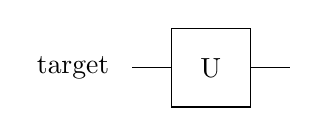
\begin{tikzpicture}[scale=.5] \node[draw=none] at (-3.5, 0) {target}; \draw (-2,0) -- (-1, 0); \draw (1, 0) -- (2, 0); \draw (-1,-1)--(-1,1)--(1,1)--(1,-1)--cycle; \node[draw=none] at (0, 0) {U}; \end{tikzpicture} } \]


\begin{DoxyParams}[1]{Parameters}
\mbox{\tt in,out}  & {\em multi\+Qubit} & object representing the set of all qubits \\
\hline
\mbox{\tt in}  & {\em target\+Qubit} & qubit to operate on \\
\hline
\mbox{\tt in}  & {\em alpha} & complex unitary parameter (row 1, column 1) \\
\hline
\mbox{\tt in}  & {\em beta} & complex unitary parameter (row 2, column 1) \\
\hline
\end{DoxyParams}

\begin{DoxyExceptions}{Exceptions}
{\em exit\+With\+Error} & if {\ttfamily target\+Qubit} is outside \mbox{[}0, {\ttfamily multi\+Qubit.\+num\+Qubits}), or if {\ttfamily alpha}, {\ttfamily beta} don\textquotesingle{}t satisfy $\vert${\ttfamily alpha$\vert$$^\wedge$2} + $\vert${\ttfamily beta$\vert$$^\wedge$2} = 1. \\
\hline
\end{DoxyExceptions}


Definition at line 98 of file Qu\+E\+S\+T\+\_\+env\+\_\+local.\+c.



Referenced by main(), rotate\+Around\+Axis(), test\+\_\+compact\+Unitary(), and test\+\_\+unitary().


\begin{DoxyCode}
99 \{
100     \mbox{\hyperlink{QuEST__env__local_8c_a3587b9d533e633ccf1abf9ad2ce45d8d}{QuESTAssert}}(targetQubit >= 0 && targetQubit < multiQubit.
      \mbox{\hyperlink{structMultiQubit_ab5b9795bdc6fb5855e1974dcbbaeb36f}{numQubits}}, 1, \_\_func\_\_);
101     \mbox{\hyperlink{QuEST__env__local_8c_a3587b9d533e633ccf1abf9ad2ce45d8d}{QuESTAssert}}(\mbox{\hyperlink{QuEST_8c_ae2b2c14a07dd7d50ff86032a3ca101d7}{validateAlphaBeta}}(alpha, beta), 6, \_\_func\_\_);
102 
103     \textcolor{comment}{// all values required to update state vector lie in this rank}
104     \mbox{\hyperlink{QuEST_8c_a9cee2d8716667a3318420a3b672f5b92}{compactUnitaryLocal}}(multiQubit, targetQubit, alpha, beta);
105 \}
\end{DoxyCode}
\mbox{\Hypertarget{QuEST__env__local_8c_ab4812953bc457405b3aa05a4c2f64f4a}\label{QuEST__env__local_8c_ab4812953bc457405b3aa05a4c2f64f4a}} 
\index{Qu\+E\+S\+T\+\_\+env\+\_\+local.\+c@{Qu\+E\+S\+T\+\_\+env\+\_\+local.\+c}!controlled\+Compact\+Unitary@{controlled\+Compact\+Unitary}}
\index{controlled\+Compact\+Unitary@{controlled\+Compact\+Unitary}!Qu\+E\+S\+T\+\_\+env\+\_\+local.\+c@{Qu\+E\+S\+T\+\_\+env\+\_\+local.\+c}}
\paragraph{\texorpdfstring{controlled\+Compact\+Unitary()}{controlledCompactUnitary()}}
{\footnotesize\ttfamily void controlled\+Compact\+Unitary (\begin{DoxyParamCaption}\item[{\mbox{\hyperlink{structMultiQubit}{Multi\+Qubit}}}]{multi\+Qubit,  }\item[{const int}]{control\+Qubit,  }\item[{const int}]{target\+Qubit,  }\item[{\mbox{\hyperlink{structComplex}{Complex}}}]{alpha,  }\item[{\mbox{\hyperlink{structComplex}{Complex}}}]{beta }\end{DoxyParamCaption})}



Apply a controlled unitary (single control, single target) parameterised by two given complex scalars. 

Given valid complex numbers $\alpha$ and $\beta$, applies the two-\/qubit unitary \[ \begin{pmatrix} 1 \\ & 1 \\ & & \alpha & -\beta^* \\ & & \beta & \alpha^* \end{pmatrix} \] to the control and target qubits. Valid $\alpha$, $\beta$ satisfy $|\alpha|^2 + |\beta|^2 = 1$. The target unitary is general up to a global phase factor. ~\newline
 \[ \setlength{\fboxrule}{0.01pt} \fbox{ 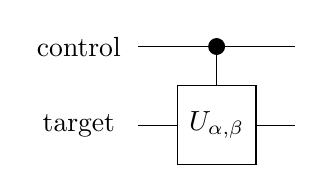
\begin{tikzpicture}[scale=.5] \node[draw=none] at (-3.5, 2) {control}; \node[draw=none] at (-3.5, 0) {target}; \draw (-2, 2) -- (2, 2); \draw[fill=black] (0, 2) circle (.2); \draw (0, 2) -- (0, 1); \draw (-2,0) -- (-1, 0); \draw (1, 0) -- (2, 0); \draw (-1,-1)--(-1,1)--(1,1)--(1,-1)--cycle; \node[draw=none] at (0, 0) {$U_{\alpha, \beta}$}; \end{tikzpicture} } \]


\begin{DoxyParams}[1]{Parameters}
\mbox{\tt in,out}  & {\em multi\+Qubit} & object representing the set of all qubits \\
\hline
\mbox{\tt in}  & {\em control\+Qubit} & apply the target unitary if this qubit has value 1 \\
\hline
\mbox{\tt in}  & {\em target\+Qubit} & qubit on which to apply the target unitary \\
\hline
\mbox{\tt in}  & {\em alpha} & complex unitary parameter (row 1, column 1) \\
\hline
\mbox{\tt in}  & {\em beta} & complex unitary parameter (row 2, column 1) \\
\hline
\end{DoxyParams}

\begin{DoxyExceptions}{Exceptions}
{\em exit\+With\+Error} & if either {\ttfamily control\+Qubit} or {\ttfamily target\+Qubit} are outside \mbox{[}0, {\ttfamily multi\+Qubit.\+num\+Qubits}) or are equal, or if {\ttfamily alpha}, {\ttfamily beta} don\textquotesingle{}t satisfy $\vert${\ttfamily alpha$\vert$$^\wedge$2} + $\vert${\ttfamily beta$\vert$$^\wedge$2} = 1. \\
\hline
\end{DoxyExceptions}


Definition at line 116 of file Qu\+E\+S\+T\+\_\+env\+\_\+local.\+c.



Referenced by controlled\+Rotate\+Around\+Axis(), main(), test\+\_\+controlled\+Compact\+Unitary(), test\+\_\+controlled\+Unitary(), and test\+\_\+multi\+Controlled\+Unitary().


\begin{DoxyCode}
117 \{
118     \mbox{\hyperlink{QuEST__env__local_8c_a3587b9d533e633ccf1abf9ad2ce45d8d}{QuESTAssert}}(targetQubit >= 0 && targetQubit < multiQubit.
      \mbox{\hyperlink{structMultiQubit_ab5b9795bdc6fb5855e1974dcbbaeb36f}{numQubits}}, 1, \_\_func\_\_);
119     \mbox{\hyperlink{QuEST__env__local_8c_a3587b9d533e633ccf1abf9ad2ce45d8d}{QuESTAssert}}(controlQubit >= 0 && controlQubit < multiQubit.
      \mbox{\hyperlink{structMultiQubit_ab5b9795bdc6fb5855e1974dcbbaeb36f}{numQubits}}, 2, \_\_func\_\_);
120     \mbox{\hyperlink{QuEST__env__local_8c_a3587b9d533e633ccf1abf9ad2ce45d8d}{QuESTAssert}}(controlQubit != targetQubit, 3, \_\_func\_\_);
121     \mbox{\hyperlink{QuEST__env__local_8c_a3587b9d533e633ccf1abf9ad2ce45d8d}{QuESTAssert}}(\mbox{\hyperlink{QuEST_8c_ae2b2c14a07dd7d50ff86032a3ca101d7}{validateAlphaBeta}}(alpha, beta), 6, \_\_func\_\_);
122 
123 
124     \mbox{\hyperlink{QuEST_8c_afc77657651d52c47403b44b923a098a8}{controlledCompactUnitaryLocal}}(multiQubit, controlQubit, targetQubit, alpha
      , beta);
125 \}
\end{DoxyCode}
\mbox{\Hypertarget{QuEST__env__local_8c_a67576895bbc65463481a8ea24d9b1e22}\label{QuEST__env__local_8c_a67576895bbc65463481a8ea24d9b1e22}} 
\index{Qu\+E\+S\+T\+\_\+env\+\_\+local.\+c@{Qu\+E\+S\+T\+\_\+env\+\_\+local.\+c}!controlled\+Not@{controlled\+Not}}
\index{controlled\+Not@{controlled\+Not}!Qu\+E\+S\+T\+\_\+env\+\_\+local.\+c@{Qu\+E\+S\+T\+\_\+env\+\_\+local.\+c}}
\paragraph{\texorpdfstring{controlled\+Not()}{controlledNot()}}
{\footnotesize\ttfamily void controlled\+Not (\begin{DoxyParamCaption}\item[{\mbox{\hyperlink{structMultiQubit}{Multi\+Qubit}}}]{multi\+Qubit,  }\item[{const int}]{control\+Qubit,  }\item[{const int}]{target\+Qubit }\end{DoxyParamCaption})}



Apply the controlled not (single control, single target) gate, also known as the c-\/X, c-\/sigma-\/X, c-\/\+Pauli-\/X and c-\/bit-\/flip gate. 

This applies sigmaX to the target qubit if the control qubit has value 1. This effects the two-\/qubit unitary \[ \begin{pmatrix} 1 \\ & 1 \\\ & & & 1 \\ & & 1 \end{pmatrix} \] on the control and target qubits.

\[ \setlength{\fboxrule}{0.01pt} \fbox{ 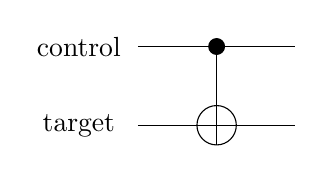
\begin{tikzpicture}[scale=.5] \node[draw=none] at (-3.5, 2) {control}; \node[draw=none] at (-3.5, 0) {target}; \draw (-2, 2) -- (2, 2); \draw[fill=black] (0, 2) circle (.2); \draw (0, 2) -- (0, -.5); \draw (-2,0) -- (2, 0); \draw (0, 0) circle (.5); \end{tikzpicture} } \] ~\newline
 
\begin{DoxyParams}[1]{Parameters}
\mbox{\tt in,out}  & {\em multi\+Qubit} & object representing the set of all qubits \\
\hline
\mbox{\tt in}  & {\em control\+Qubit} & nots the target if this qubit is 1 \\
\hline
\mbox{\tt in}  & {\em target\+Qubit} & qubit to not \\
\hline
\end{DoxyParams}

\begin{DoxyExceptions}{Exceptions}
{\em exit\+With\+Error} & if either {\ttfamily control\+Qubit} or {\ttfamily target\+Qubit} are outside \mbox{[}0, {\ttfamily multi\+Qubit.\+num\+Qubits}), or are equal. \\
\hline
\end{DoxyExceptions}


Definition at line 175 of file Qu\+E\+S\+T\+\_\+env\+\_\+local.\+c.



Referenced by main(), and test\+\_\+controlled\+Not().


\begin{DoxyCode}
176 \{
177     \mbox{\hyperlink{QuEST__env__local_8c_a3587b9d533e633ccf1abf9ad2ce45d8d}{QuESTAssert}}(targetQubit >= 0 && targetQubit < multiQubit.
      \mbox{\hyperlink{structMultiQubit_ab5b9795bdc6fb5855e1974dcbbaeb36f}{numQubits}}, 1, \_\_func\_\_);
178     \mbox{\hyperlink{QuEST__env__local_8c_a3587b9d533e633ccf1abf9ad2ce45d8d}{QuESTAssert}}(controlQubit >= 0 && controlQubit < multiQubit.
      \mbox{\hyperlink{structMultiQubit_ab5b9795bdc6fb5855e1974dcbbaeb36f}{numQubits}}, 2, \_\_func\_\_);
179     \mbox{\hyperlink{QuEST__env__local_8c_a3587b9d533e633ccf1abf9ad2ce45d8d}{QuESTAssert}}(controlQubit != targetQubit, 3, \_\_func\_\_);
180     \mbox{\hyperlink{QuEST_8c_ad357a43e80e3baf013975b1b70942f4c}{controlledNotLocal}}(multiQubit, controlQubit, targetQubit);
181 \}
\end{DoxyCode}
\mbox{\Hypertarget{QuEST__env__local_8c_a8a701526263392599aa21d0d0f05d9d8}\label{QuEST__env__local_8c_a8a701526263392599aa21d0d0f05d9d8}} 
\index{Qu\+E\+S\+T\+\_\+env\+\_\+local.\+c@{Qu\+E\+S\+T\+\_\+env\+\_\+local.\+c}!controlled\+Unitary@{controlled\+Unitary}}
\index{controlled\+Unitary@{controlled\+Unitary}!Qu\+E\+S\+T\+\_\+env\+\_\+local.\+c@{Qu\+E\+S\+T\+\_\+env\+\_\+local.\+c}}
\paragraph{\texorpdfstring{controlled\+Unitary()}{controlledUnitary()}}
{\footnotesize\ttfamily void controlled\+Unitary (\begin{DoxyParamCaption}\item[{\mbox{\hyperlink{structMultiQubit}{Multi\+Qubit}}}]{multi\+Qubit,  }\item[{const int}]{control\+Qubit,  }\item[{const int}]{target\+Qubit,  }\item[{\mbox{\hyperlink{structComplexMatrix2}{Complex\+Matrix2}}}]{u }\end{DoxyParamCaption})}



Apply a general controlled unitary (single control, single target), which can include a global phase factor. 

The given unitary is applied to the target qubit if the control qubit has value 1, effecting the two-\/qubit unitary \[ \begin{pmatrix} 1 \\ & 1 \\ & & u_{00} & u_{01}\\ & & u_{10} & u_{11} \end{pmatrix} \] on the control and target qubits.

\[ \setlength{\fboxrule}{0.01pt} \fbox{ 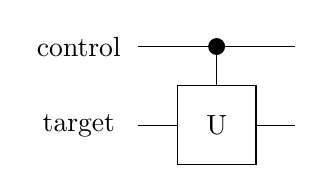
\begin{tikzpicture}[scale=.5] \node[draw=none] at (-3.5, 2) {control}; \node[draw=none] at (-3.5, 0) {target}; \draw (-2, 2) -- (2, 2); \draw[fill=black] (0, 2) circle (.2); \draw (0, 2) -- (0, 1); \draw (-2,0) -- (-1, 0); \draw (1, 0) -- (2, 0); \draw (-1,-1)--(-1,1)--(1,1)--(1,-1)--cycle; \node[draw=none] at (0, 0) {U}; \end{tikzpicture} } \]


\begin{DoxyParams}[1]{Parameters}
\mbox{\tt in,out}  & {\em multi\+Qubit} & object representing the set of all qubits \\
\hline
\mbox{\tt in}  & {\em control\+Qubit} & apply unitary if this qubit is 1 \\
\hline
\mbox{\tt in}  & {\em target\+Qubit} & qubit to operate on \\
\hline
\mbox{\tt in}  & {\em u} & single-\/qubit unitary matrix to apply \\
\hline
\end{DoxyParams}

\begin{DoxyExceptions}{Exceptions}
{\em exit\+With\+Error} & if either {\ttfamily control\+Qubit} or {\ttfamily target\+Qubit} are outside \mbox{[}0, {\ttfamily multi\+Qubit.\+num\+Qubits}) or are equal, or if {\ttfamily u} is not unitary. \\
\hline
\end{DoxyExceptions}


Definition at line 127 of file Qu\+E\+S\+T\+\_\+env\+\_\+local.\+c.



Referenced by test\+\_\+controlled\+Unitary().


\begin{DoxyCode}
128 \{
129     \mbox{\hyperlink{QuEST__env__local_8c_a3587b9d533e633ccf1abf9ad2ce45d8d}{QuESTAssert}}(targetQubit >= 0 && targetQubit < multiQubit.
      \mbox{\hyperlink{structMultiQubit_ab5b9795bdc6fb5855e1974dcbbaeb36f}{numQubits}}, 1, \_\_func\_\_);
130     \mbox{\hyperlink{QuEST__env__local_8c_a3587b9d533e633ccf1abf9ad2ce45d8d}{QuESTAssert}}(controlQubit >= 0 && controlQubit < multiQubit.
      \mbox{\hyperlink{structMultiQubit_ab5b9795bdc6fb5855e1974dcbbaeb36f}{numQubits}}, 2, \_\_func\_\_);
131     \mbox{\hyperlink{QuEST__env__local_8c_a3587b9d533e633ccf1abf9ad2ce45d8d}{QuESTAssert}}(controlQubit != targetQubit, 3, \_\_func\_\_);
132     \mbox{\hyperlink{QuEST__env__local_8c_a3587b9d533e633ccf1abf9ad2ce45d8d}{QuESTAssert}}(\mbox{\hyperlink{QuEST_8c_ae4fea133d1a8f09ff8da03038100adb2}{validateMatrixIsUnitary}}(u), 5, \_\_func\_\_);
133 
134     \mbox{\hyperlink{QuEST_8c_a8a4afcff70195a306c082b8ed8d4e09a}{controlledUnitaryLocal}}(multiQubit, controlQubit, targetQubit, u);
135 \}
\end{DoxyCode}
\mbox{\Hypertarget{QuEST__env__local_8c_ae5f9019826f35e8b51b1716cfe397b45}\label{QuEST__env__local_8c_ae5f9019826f35e8b51b1716cfe397b45}} 
\index{Qu\+E\+S\+T\+\_\+env\+\_\+local.\+c@{Qu\+E\+S\+T\+\_\+env\+\_\+local.\+c}!exit\+With\+Error@{exit\+With\+Error}}
\index{exit\+With\+Error@{exit\+With\+Error}!Qu\+E\+S\+T\+\_\+env\+\_\+local.\+c@{Qu\+E\+S\+T\+\_\+env\+\_\+local.\+c}}
\paragraph{\texorpdfstring{exit\+With\+Error()}{exitWithError()}}
{\footnotesize\ttfamily void exit\+With\+Error (\begin{DoxyParamCaption}\item[{int}]{error\+Code,  }\item[{const char $\ast$}]{func }\end{DoxyParamCaption})}



Definition at line 232 of file Qu\+E\+S\+T\+\_\+env\+\_\+local.\+c.



Referenced by Qu\+E\+S\+T\+Assert().


\begin{DoxyCode}
232                                                    \{
233     printf(\textcolor{stringliteral}{"!!!\(\backslash\)n"});
234     printf(\textcolor{stringliteral}{"QuEST Error in function %s: %s\(\backslash\)n"}, func, \mbox{\hyperlink{QuEST_8c_aac1637696885c75b73a1ecf381cea713}{errorCodes}}[errorCode]);
235     printf(\textcolor{stringliteral}{"!!!\(\backslash\)n"});
236     printf(\textcolor{stringliteral}{"exiting..\(\backslash\)n"});
237     exit(errorCode);
238 \}
\end{DoxyCode}
\mbox{\Hypertarget{QuEST__env__local_8c_ad315c941a51bc053d39ebfa2040fd32e}\label{QuEST__env__local_8c_ad315c941a51bc053d39ebfa2040fd32e}} 
\index{Qu\+E\+S\+T\+\_\+env\+\_\+local.\+c@{Qu\+E\+S\+T\+\_\+env\+\_\+local.\+c}!find\+Probability\+Of\+Outcome@{find\+Probability\+Of\+Outcome}}
\index{find\+Probability\+Of\+Outcome@{find\+Probability\+Of\+Outcome}!Qu\+E\+S\+T\+\_\+env\+\_\+local.\+c@{Qu\+E\+S\+T\+\_\+env\+\_\+local.\+c}}
\paragraph{\texorpdfstring{find\+Probability\+Of\+Outcome()}{findProbabilityOfOutcome()}}
{\footnotesize\ttfamily \mbox{\hyperlink{QuEST__precision_8h_a4b654506f18b8bfd61ad2a29a7e38c25}{R\+E\+AL}} find\+Probability\+Of\+Outcome (\begin{DoxyParamCaption}\item[{\mbox{\hyperlink{structMultiQubit}{Multi\+Qubit}}}]{multi\+Qubit,  }\item[{const int}]{measure\+Qubit,  }\item[{int}]{outcome }\end{DoxyParamCaption})}



Gives the probability of a specified qubit being measured in the given outcome (0 or 1). 

This performs no actual measurement and does not change the state of the qubits.


\begin{DoxyParams}[1]{Parameters}
\mbox{\tt in}  & {\em multi\+Qubit} & object representing the set of all qubits \\
\hline
\mbox{\tt in}  & {\em measure\+Qubit} & qubit to study \\
\hline
\mbox{\tt in}  & {\em outcome} & for which to find the probability of the qubit being measured in \\
\hline
\end{DoxyParams}
\begin{DoxyReturn}{Returns}
probability of qubit measure\+Qubit being measured in the given outcome 
\end{DoxyReturn}

\begin{DoxyExceptions}{Exceptions}
{\em exit\+With\+Error} & if {\ttfamily measure\+Qubit} is outside \mbox{[}0, {\ttfamily multi\+Qubit.\+num\+Qubits}), or if {\ttfamily outcome} is not in \{0, 1\}. \\
\hline
\end{DoxyExceptions}


Definition at line 183 of file Qu\+E\+S\+T\+\_\+env\+\_\+local.\+c.



Referenced by collapse\+To\+Outcome(), main(), measure\+With\+Stats(), and test\+\_\+find\+Probability\+Of\+Outcome().


\begin{DoxyCode}
184 \{
185     \mbox{\hyperlink{QuEST__env__local_8c_a3587b9d533e633ccf1abf9ad2ce45d8d}{QuESTAssert}}(measureQubit >= 0 && measureQubit < multiQubit.
      \mbox{\hyperlink{structMultiQubit_ab5b9795bdc6fb5855e1974dcbbaeb36f}{numQubits}}, 2, \_\_func\_\_);
186     \mbox{\hyperlink{QuEST__precision_8h_a4b654506f18b8bfd61ad2a29a7e38c25}{REAL}} stateProb=0;
187     stateProb = \mbox{\hyperlink{QuEST_8c_a7c02cd0e1b4eac19771a0525f023249e}{findProbabilityOfZeroLocal}}(multiQubit, measureQubit);
188     \textcolor{keywordflow}{if} (outcome==1) stateProb = 1.0 - stateProb;
189     \textcolor{keywordflow}{return} stateProb;
190 \}
\end{DoxyCode}
\mbox{\Hypertarget{QuEST__env__local_8c_a3615f76fd5f57008d9b74bbd10533dd0}\label{QuEST__env__local_8c_a3615f76fd5f57008d9b74bbd10533dd0}} 
\index{Qu\+E\+S\+T\+\_\+env\+\_\+local.\+c@{Qu\+E\+S\+T\+\_\+env\+\_\+local.\+c}!get\+Imag\+Amp\+El@{get\+Imag\+Amp\+El}}
\index{get\+Imag\+Amp\+El@{get\+Imag\+Amp\+El}!Qu\+E\+S\+T\+\_\+env\+\_\+local.\+c@{Qu\+E\+S\+T\+\_\+env\+\_\+local.\+c}}
\paragraph{\texorpdfstring{get\+Imag\+Amp\+El()}{getImagAmpEl()}}
{\footnotesize\ttfamily \mbox{\hyperlink{QuEST__precision_8h_a4b654506f18b8bfd61ad2a29a7e38c25}{R\+E\+AL}} get\+Imag\+Amp\+El (\begin{DoxyParamCaption}\item[{\mbox{\hyperlink{structMultiQubit}{Multi\+Qubit}}}]{multi\+Qubit,  }\item[{long long int}]{index }\end{DoxyParamCaption})}



Get the imaginary component of the complex probability amplitude at an index in the state vector. 

For debugging purposes.


\begin{DoxyParams}[1]{Parameters}
\mbox{\tt in}  & {\em multi\+Qubit} & object representing a set of qubits \\
\hline
\mbox{\tt in}  & {\em index} & index in state vector of probability amplitudes \\
\hline
\end{DoxyParams}
\begin{DoxyReturn}{Returns}
imaginary component at that index 
\end{DoxyReturn}

\begin{DoxyExceptions}{Exceptions}
{\em exit\+With\+Error} & if {\ttfamily index} is outside \mbox{[}0, $2^{N}$) where $N = $ {\ttfamily multi\+Qubit.\+num\+Qubits} \\
\hline
\end{DoxyExceptions}


Definition at line 94 of file Qu\+E\+S\+T\+\_\+env\+\_\+local.\+c.



Referenced by get\+Prob\+El(), and test\+\_\+get\+Imag\+Amp\+El().


\begin{DoxyCode}
94                                                              \{
95     \textcolor{keywordflow}{return} multiQubit.\mbox{\hyperlink{structMultiQubit_a45483190d6b01ef6b2f98f2bec9ab94f}{stateVec}}.\mbox{\hyperlink{structComplexArray_a79dde47c7ae530c79cebfdf57b225968}{imag}}[index];
96 \}
\end{DoxyCode}
\mbox{\Hypertarget{QuEST__env__local_8c_a317b786f577fa6bc136ea7f0ee7330a7}\label{QuEST__env__local_8c_a317b786f577fa6bc136ea7f0ee7330a7}} 
\index{Qu\+E\+S\+T\+\_\+env\+\_\+local.\+c@{Qu\+E\+S\+T\+\_\+env\+\_\+local.\+c}!get\+Real\+Amp\+El@{get\+Real\+Amp\+El}}
\index{get\+Real\+Amp\+El@{get\+Real\+Amp\+El}!Qu\+E\+S\+T\+\_\+env\+\_\+local.\+c@{Qu\+E\+S\+T\+\_\+env\+\_\+local.\+c}}
\paragraph{\texorpdfstring{get\+Real\+Amp\+El()}{getRealAmpEl()}}
{\footnotesize\ttfamily \mbox{\hyperlink{QuEST__precision_8h_a4b654506f18b8bfd61ad2a29a7e38c25}{R\+E\+AL}} get\+Real\+Amp\+El (\begin{DoxyParamCaption}\item[{\mbox{\hyperlink{structMultiQubit}{Multi\+Qubit}}}]{multi\+Qubit,  }\item[{long long int}]{index }\end{DoxyParamCaption})}



Get the real component of the complex probability amplitude at an index in the state vector. 

For debugging purposes.


\begin{DoxyParams}[1]{Parameters}
\mbox{\tt in}  & {\em multi\+Qubit} & object representing a set of qubits \\
\hline
\mbox{\tt in}  & {\em index} & index in state vector of probability amplitudes \\
\hline
\end{DoxyParams}
\begin{DoxyReturn}{Returns}
real component at that index 
\end{DoxyReturn}

\begin{DoxyExceptions}{Exceptions}
{\em exit\+With\+Error} & if {\ttfamily index} is outside \mbox{[}0, $2^{N}$) where $N = $ {\ttfamily multi\+Qubit.\+num\+Qubits} \\
\hline
\end{DoxyExceptions}


Definition at line 90 of file Qu\+E\+S\+T\+\_\+env\+\_\+local.\+c.



Referenced by get\+Prob\+El(), and test\+\_\+get\+Real\+Amp\+El().


\begin{DoxyCode}
90                                                              \{
91     \textcolor{keywordflow}{return} multiQubit.\mbox{\hyperlink{structMultiQubit_a45483190d6b01ef6b2f98f2bec9ab94f}{stateVec}}.\mbox{\hyperlink{structComplexArray_a4195cac6c784ea1b6271f1c7dba1548a}{real}}[index];
92 \}
\end{DoxyCode}
\mbox{\Hypertarget{QuEST__env__local_8c_aa09b5dd93de6df1384b8f2c0041749ab}\label{QuEST__env__local_8c_aa09b5dd93de6df1384b8f2c0041749ab}} 
\index{Qu\+E\+S\+T\+\_\+env\+\_\+local.\+c@{Qu\+E\+S\+T\+\_\+env\+\_\+local.\+c}!hadamard@{hadamard}}
\index{hadamard@{hadamard}!Qu\+E\+S\+T\+\_\+env\+\_\+local.\+c@{Qu\+E\+S\+T\+\_\+env\+\_\+local.\+c}}
\paragraph{\texorpdfstring{hadamard()}{hadamard()}}
{\footnotesize\ttfamily void hadamard (\begin{DoxyParamCaption}\item[{\mbox{\hyperlink{structMultiQubit}{Multi\+Qubit}}}]{multi\+Qubit,  }\item[{const int}]{target\+Qubit }\end{DoxyParamCaption})}



Apply the single-\/qubit Hadamard gate. 

This takes $|0\rangle$ to $|+\rangle$ and $|1\rangle$ to $|-\rangle$, and is equivalent to a rotation of $\pi$ around the x-\/axis then $\pi/2$ about the y-\/axis on the Bloch-\/sphere. I.\+e. \[ \frac{1}{\sqrt{2}} \begin{pmatrix} 1 & 1 \\ 1 & -1 \end{pmatrix} \] ~\newline
 \[ \setlength{\fboxrule}{0.01pt} \fbox{ 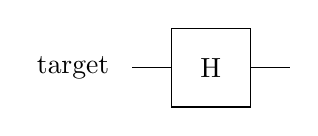
\begin{tikzpicture}[scale=.5] \node[draw=none] at (-3.5, 0) {target}; \draw (-2,0) -- (-1, 0); \draw (1, 0) -- (2, 0); \draw (-1,-1)--(-1,1)--(1,1)--(1,-1)--cycle; \node[draw=none] at (0, 0) {H}; \end{tikzpicture} } \] ~\newline
 
\begin{DoxyParams}[1]{Parameters}
\mbox{\tt in,out}  & {\em multi\+Qubit} & object representing the set of all qubits \\
\hline
\mbox{\tt in}  & {\em target\+Qubit} & qubit to operate on \\
\hline
\end{DoxyParams}

\begin{DoxyExceptions}{Exceptions}
{\em exit\+With\+Error} & if {\ttfamily target\+Qubit} is outside \mbox{[}0, {\ttfamily multi\+Qubit.\+num\+Qubits}). \\
\hline
\end{DoxyExceptions}


Definition at line 169 of file Qu\+E\+S\+T\+\_\+env\+\_\+local.\+c.



Referenced by main(), and test\+\_\+hadamard().


\begin{DoxyCode}
170 \{
171     \mbox{\hyperlink{QuEST__env__local_8c_a3587b9d533e633ccf1abf9ad2ce45d8d}{QuESTAssert}}(targetQubit >= 0 && targetQubit < multiQubit.
      \mbox{\hyperlink{structMultiQubit_ab5b9795bdc6fb5855e1974dcbbaeb36f}{numQubits}}, 1, \_\_func\_\_);
172     \mbox{\hyperlink{QuEST_8c_aa9f0718b4dd794a3e1b143e3b153bfc5}{hadamardLocal}}(multiQubit, targetQubit);
173 \}
\end{DoxyCode}
\mbox{\Hypertarget{QuEST__env__local_8c_ad84a3ce68d1ca02b4e3f741ea45b6054}\label{QuEST__env__local_8c_ad84a3ce68d1ca02b4e3f741ea45b6054}} 
\index{Qu\+E\+S\+T\+\_\+env\+\_\+local.\+c@{Qu\+E\+S\+T\+\_\+env\+\_\+local.\+c}!init\+Qu\+E\+S\+T\+Env@{init\+Qu\+E\+S\+T\+Env}}
\index{init\+Qu\+E\+S\+T\+Env@{init\+Qu\+E\+S\+T\+Env}!Qu\+E\+S\+T\+\_\+env\+\_\+local.\+c@{Qu\+E\+S\+T\+\_\+env\+\_\+local.\+c}}
\paragraph{\texorpdfstring{init\+Qu\+E\+S\+T\+Env()}{initQuESTEnv()}}
{\footnotesize\ttfamily void init\+Qu\+E\+S\+T\+Env (\begin{DoxyParamCaption}\item[{\mbox{\hyperlink{structQuESTEnv}{Qu\+E\+S\+T\+Env}} $\ast$}]{env }\end{DoxyParamCaption})}



Initialize the Qu\+E\+ST environment. 

If something needs to be done to set up the execution environment, such as initializing M\+PI when running in distributed mode, it is handled here


\begin{DoxyParams}[1]{Parameters}
\mbox{\tt in,out}  & {\em env} & object representing the execution environment. A single instance is used for each program \\
\hline
\end{DoxyParams}


Definition at line 23 of file Qu\+E\+S\+T\+\_\+env\+\_\+local.\+c.



Referenced by main().


\begin{DoxyCode}
23                                 \{
24     \textcolor{comment}{// init MPI environment}
25     \mbox{\hyperlink{runTests_8c_a5fd8ba97fcae3408ae6221dfc3cc1f93}{env}}->\mbox{\hyperlink{structQuESTEnv_aa648bb336cf8598467cb62db00b9cee8}{rank}}=0;
26     \mbox{\hyperlink{runTests_8c_a5fd8ba97fcae3408ae6221dfc3cc1f93}{env}}->\mbox{\hyperlink{structQuESTEnv_af22aacd7c9905accae28484785c193b4}{numRanks}}=1;
27         
28         \mbox{\hyperlink{QuEST_8c_ab0ab3ec70938712c26988a6aa51263a0}{seedQuESTDefault}}();
29 \}
\end{DoxyCode}
\mbox{\Hypertarget{QuEST__env__local_8c_ad5774247d836267175c664cd0e451bcb}\label{QuEST__env__local_8c_ad5774247d836267175c664cd0e451bcb}} 
\index{Qu\+E\+S\+T\+\_\+env\+\_\+local.\+c@{Qu\+E\+S\+T\+\_\+env\+\_\+local.\+c}!measure@{measure}}
\index{measure@{measure}!Qu\+E\+S\+T\+\_\+env\+\_\+local.\+c@{Qu\+E\+S\+T\+\_\+env\+\_\+local.\+c}}
\paragraph{\texorpdfstring{measure()}{measure()}}
{\footnotesize\ttfamily int measure (\begin{DoxyParamCaption}\item[{\mbox{\hyperlink{structMultiQubit}{Multi\+Qubit}}}]{multi\+Qubit,  }\item[{int}]{measure\+Qubit }\end{DoxyParamCaption})}



Measures a single qubit, collapsing it randomly to 0 or 1. 

Outcome probabilities are weighted by the state vector, which is irreversibly changed after collapse to be consistent with the outcome.


\begin{DoxyParams}[1]{Parameters}
\mbox{\tt in,out}  & {\em multi\+Qubit} & object representing the set of all qubits \\
\hline
\mbox{\tt in}  & {\em measure\+Qubit} & qubit to measure \\
\hline
\end{DoxyParams}
\begin{DoxyReturn}{Returns}
the measurement outcome, 0 or 1 
\end{DoxyReturn}

\begin{DoxyExceptions}{Exceptions}
{\em exit\+With\+Error} & if {\ttfamily measure\+Qubit} is outside \mbox{[}0, {\ttfamily multi\+Qubit.\+num\+Qubits}) \\
\hline
\end{DoxyExceptions}


Definition at line 203 of file Qu\+E\+S\+T\+\_\+env\+\_\+local.\+c.



Referenced by main(), and test\+\_\+measure().


\begin{DoxyCode}
203                                                     \{
204     \mbox{\hyperlink{QuEST__env__local_8c_a3587b9d533e633ccf1abf9ad2ce45d8d}{QuESTAssert}}(measureQubit >= 0 && measureQubit < multiQubit.
      \mbox{\hyperlink{structMultiQubit_ab5b9795bdc6fb5855e1974dcbbaeb36f}{numQubits}}, 2, \_\_func\_\_);
205     \mbox{\hyperlink{QuEST__precision_8h_a4b654506f18b8bfd61ad2a29a7e38c25}{REAL}} stateProb;
206     \textcolor{keywordflow}{return} \mbox{\hyperlink{QuEST__env__local_8c_a2ac46e470c750bf93c754e06c64b0a7a}{measureWithStats}}(multiQubit, measureQubit, &stateProb);
207 \}
\end{DoxyCode}
\mbox{\Hypertarget{QuEST__env__local_8c_a2ac46e470c750bf93c754e06c64b0a7a}\label{QuEST__env__local_8c_a2ac46e470c750bf93c754e06c64b0a7a}} 
\index{Qu\+E\+S\+T\+\_\+env\+\_\+local.\+c@{Qu\+E\+S\+T\+\_\+env\+\_\+local.\+c}!measure\+With\+Stats@{measure\+With\+Stats}}
\index{measure\+With\+Stats@{measure\+With\+Stats}!Qu\+E\+S\+T\+\_\+env\+\_\+local.\+c@{Qu\+E\+S\+T\+\_\+env\+\_\+local.\+c}}
\paragraph{\texorpdfstring{measure\+With\+Stats()}{measureWithStats()}}
{\footnotesize\ttfamily int measure\+With\+Stats (\begin{DoxyParamCaption}\item[{\mbox{\hyperlink{structMultiQubit}{Multi\+Qubit}}}]{multi\+Qubit,  }\item[{int}]{measure\+Qubit,  }\item[{\mbox{\hyperlink{QuEST__precision_8h_a4b654506f18b8bfd61ad2a29a7e38c25}{R\+E\+AL}} $\ast$}]{state\+Prob }\end{DoxyParamCaption})}



Measures a single qubit, collapsing it randomly to 0 or 1, and additionally gives the probability of that outcome. 

Outcome probabilities are weighted by the state vector, which is irreversibly changed after collapse to be consistent with the outcome.


\begin{DoxyParams}[1]{Parameters}
\mbox{\tt in,out}  & {\em multi\+Qubit} & object representing the set of all qubits \\
\hline
\mbox{\tt in}  & {\em measure\+Qubit} & qubit to measure \\
\hline
\mbox{\tt out}  & {\em state\+Prob} & a pointer to a R\+E\+AL which is set to the probability of the occurred outcome \\
\hline
\end{DoxyParams}
\begin{DoxyReturn}{Returns}
the measurement outcome, 0 or 1 
\end{DoxyReturn}

\begin{DoxyExceptions}{Exceptions}
{\em exit\+With\+Error} & if {\ttfamily measure\+Qubit} is outside \mbox{[}0, {\ttfamily multi\+Qubit.\+num\+Qubits}) \\
\hline
\end{DoxyExceptions}


Definition at line 209 of file Qu\+E\+S\+T\+\_\+env\+\_\+local.\+c.



Referenced by main(), measure(), and test\+\_\+measure\+With\+Stats().


\begin{DoxyCode}
209                                                                               \{
210     \mbox{\hyperlink{QuEST__env__local_8c_a3587b9d533e633ccf1abf9ad2ce45d8d}{QuESTAssert}}(measureQubit >= 0 && measureQubit < multiQubit.
      \mbox{\hyperlink{structMultiQubit_ab5b9795bdc6fb5855e1974dcbbaeb36f}{numQubits}}, 2, \_\_func\_\_);
211 
212     \textcolor{keywordtype}{int} outcome;
213     \textcolor{comment}{// find probability of qubit being in state 1}
214     \mbox{\hyperlink{QuEST__precision_8h_a4b654506f18b8bfd61ad2a29a7e38c25}{REAL}} stateProbInternal = \mbox{\hyperlink{QuEST__env__local_8c_ad315c941a51bc053d39ebfa2040fd32e}{findProbabilityOfOutcome}}(multiQubit, measureQubit,
       1);
215 
216     \textcolor{comment}{// we can't collapse to a state that has a probability too close to zero}
217     \textcolor{keywordflow}{if} (stateProbInternal<\mbox{\hyperlink{QuEST__precision_8h_aebb5e6716e06431296af4d1a71744dec}{REAL\_EPS}}) outcome=0;
218     \textcolor{keywordflow}{else} \textcolor{keywordflow}{if} (1-stateProbInternal<\mbox{\hyperlink{QuEST__precision_8h_aebb5e6716e06431296af4d1a71744dec}{REAL\_EPS}}) outcome=1;
219     \textcolor{keywordflow}{else} \{
220         \textcolor{comment}{// ok. both P(0) and P(1) are large enough to resolve}
221         \textcolor{comment}{// generate random float on [0,1]}
222         \textcolor{keywordtype}{float} randNum = \mbox{\hyperlink{mt19937ar_8c_ac94ab75771800274ed1a2bedeca86f04}{genrand\_real1}}();
223         \textcolor{keywordflow}{if} (randNum<=stateProbInternal) outcome = 1;
224         \textcolor{keywordflow}{else} outcome = 0;
225     \} 
226     \textcolor{keywordflow}{if} (outcome==0) stateProbInternal = 1-stateProbInternal;
227     \mbox{\hyperlink{QuEST_8c_a01d9a8b7ff0e09ec399e158389783aa9}{collapseToOutcomeLocal}}(multiQubit, measureQubit, stateProbInternal, outcome);
228     *stateProb = stateProbInternal;
229     \textcolor{keywordflow}{return} outcome;
230 \}
\end{DoxyCode}
\mbox{\Hypertarget{QuEST__env__local_8c_ae395a79690283ed81106afadd7a8cd8a}\label{QuEST__env__local_8c_ae395a79690283ed81106afadd7a8cd8a}} 
\index{Qu\+E\+S\+T\+\_\+env\+\_\+local.\+c@{Qu\+E\+S\+T\+\_\+env\+\_\+local.\+c}!multi\+Controlled\+Unitary@{multi\+Controlled\+Unitary}}
\index{multi\+Controlled\+Unitary@{multi\+Controlled\+Unitary}!Qu\+E\+S\+T\+\_\+env\+\_\+local.\+c@{Qu\+E\+S\+T\+\_\+env\+\_\+local.\+c}}
\paragraph{\texorpdfstring{multi\+Controlled\+Unitary()}{multiControlledUnitary()}}
{\footnotesize\ttfamily void multi\+Controlled\+Unitary (\begin{DoxyParamCaption}\item[{\mbox{\hyperlink{structMultiQubit}{Multi\+Qubit}}}]{multi\+Qubit,  }\item[{int $\ast$}]{control\+Qubits,  }\item[{const int}]{num\+Control\+Qubits,  }\item[{const int}]{target\+Qubit,  }\item[{\mbox{\hyperlink{structComplexMatrix2}{Complex\+Matrix2}}}]{u }\end{DoxyParamCaption})}



Apply a general multiple-\/control single-\/target unitary, which can include a global phase factor. 

Any number of control qubits can be specified, and if all have value 1, the given unitary is applied to the target qubit. This effects the many-\/qubit unitary \[ \begin{pmatrix} 1 \\ & 1 \\\ & & \ddots \\ & & & u_{00} & u_{01}\\ & & & u_{10} & u_{11} \end{pmatrix} \] on the control and target qubits. The given 2x2 Complex\+Matrix must be unitary, otherwise an error is thrown.

\[ \setlength{\fboxrule}{0.01pt} \fbox{ 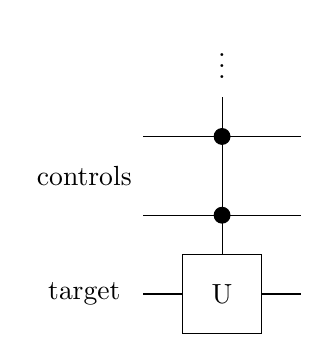
\begin{tikzpicture}[scale=.5] \node[draw=none] at (-3.5, 3) {controls}; \node[draw=none] at (-3.5, 0) {target}; \node[draw=none] at (0, 6) {$\vdots$}; \draw (0, 5) -- (0, 4); \draw (-2, 4) -- (2, 4); \draw[fill=black] (0, 4) circle (.2); \draw (0, 4) -- (0, 2); \draw (-2, 2) -- (2, 2); \draw[fill=black] (0, 2) circle (.2); \draw (0, 2) -- (0, 1); \draw (-2,0) -- (-1, 0); \draw (1, 0) -- (2, 0); \draw (-1,-1)--(-1,1)--(1,1)--(1,-1)--cycle; \node[draw=none] at (0, 0) {U}; \end{tikzpicture} } \]


\begin{DoxyParams}[1]{Parameters}
\mbox{\tt in,out}  & {\em multi\+Qubit} & object representing the set of all qubits \\
\hline
\mbox{\tt in}  & {\em control\+Qubits} & applies unitary if all qubits in this array equal 1 \\
\hline
\mbox{\tt in}  & {\em num\+Control\+Qubits} & number of control qubits \\
\hline
\mbox{\tt in}  & {\em target\+Qubit} & qubit to operate on \\
\hline
\mbox{\tt in}  & {\em u} & single-\/qubit unitary matrix to apply \\
\hline
\end{DoxyParams}

\begin{DoxyExceptions}{Exceptions}
{\em exit\+With\+Error} & if {\ttfamily num\+Control\+Qubits} is outside \mbox{[}1, {\ttfamily multi\+Qubit.\+num\+Qubits}\mbox{]}), or if any qubit index ({\ttfamily target\+Qubit} or one in {\ttfamily control\+Qubits}) is outside \mbox{[}0, {\ttfamily multi\+Qubit.\+num\+Qubits}\mbox{]}), or if {\ttfamily control\+Qubits} contains {\ttfamily target\+Qubit}, or if {\ttfamily u} is not unitary. \\
\hline
\end{DoxyExceptions}


Definition at line 137 of file Qu\+E\+S\+T\+\_\+env\+\_\+local.\+c.



Referenced by main(), and test\+\_\+multi\+Controlled\+Unitary().


\begin{DoxyCode}
138 \{
139     \mbox{\hyperlink{QuEST__env__local_8c_a3587b9d533e633ccf1abf9ad2ce45d8d}{QuESTAssert}}(targetQubit >= 0 && targetQubit < multiQubit.
      \mbox{\hyperlink{structMultiQubit_ab5b9795bdc6fb5855e1974dcbbaeb36f}{numQubits}}, 1, \_\_func\_\_);
140     \mbox{\hyperlink{QuEST__env__local_8c_a3587b9d533e633ccf1abf9ad2ce45d8d}{QuESTAssert}}(numControlQubits > 0 && numControlQubits <= multiQubit.
      \mbox{\hyperlink{structMultiQubit_ab5b9795bdc6fb5855e1974dcbbaeb36f}{numQubits}}, 4, \_\_func\_\_);
141     \mbox{\hyperlink{QuEST__env__local_8c_a3587b9d533e633ccf1abf9ad2ce45d8d}{QuESTAssert}}(\mbox{\hyperlink{QuEST_8c_ae4fea133d1a8f09ff8da03038100adb2}{validateMatrixIsUnitary}}(u), 5, \_\_func\_\_);
142 
143     \textcolor{keywordtype}{long} \textcolor{keywordtype}{long} \textcolor{keywordtype}{int} mask=0; 
144     \textcolor{keywordflow}{for} (\textcolor{keywordtype}{int} i=0; i<numControlQubits; i++) mask = mask | (1LL<<controlQubits[i]);
145     \mbox{\hyperlink{QuEST__env__local_8c_a3587b9d533e633ccf1abf9ad2ce45d8d}{QuESTAssert}}(mask >=0 && mask <= (1LL<<multiQubit.\mbox{\hyperlink{structMultiQubit_ab5b9795bdc6fb5855e1974dcbbaeb36f}{numQubits}})-1, 2, \_\_func\_\_);
146     \mbox{\hyperlink{QuEST__env__local_8c_a3587b9d533e633ccf1abf9ad2ce45d8d}{QuESTAssert}}((mask & (1LL<<targetQubit)) != (1LL<<targetQubit), 3, \_\_func\_\_);
147 
148     \mbox{\hyperlink{QuEST_8c_a1309eabcba3cb97fbc3cd2e606d17766}{multiControlledUnitaryLocal}}(multiQubit, targetQubit, mask, u);
149 \}
\end{DoxyCode}
\mbox{\Hypertarget{QuEST__env__local_8c_aae7a8a7f1ccbddb7f76b6c52b746bb43}\label{QuEST__env__local_8c_aae7a8a7f1ccbddb7f76b6c52b746bb43}} 
\index{Qu\+E\+S\+T\+\_\+env\+\_\+local.\+c@{Qu\+E\+S\+T\+\_\+env\+\_\+local.\+c}!phase\+Gate@{phase\+Gate}}
\index{phase\+Gate@{phase\+Gate}!Qu\+E\+S\+T\+\_\+env\+\_\+local.\+c@{Qu\+E\+S\+T\+\_\+env\+\_\+local.\+c}}
\paragraph{\texorpdfstring{phase\+Gate()}{phaseGate()}}
{\footnotesize\ttfamily void phase\+Gate (\begin{DoxyParamCaption}\item[{\mbox{\hyperlink{structMultiQubit}{Multi\+Qubit}}}]{multi\+Qubit,  }\item[{const int}]{target\+Qubit,  }\item[{enum \mbox{\hyperlink{QuEST_8h_a5739021c733cecc49647956b2f7338ea}{phase\+Gate\+Type}}}]{type }\end{DoxyParamCaption})}



Definition at line 163 of file Qu\+E\+S\+T\+\_\+env\+\_\+local.\+c.



Referenced by s\+Gate(), sigma\+Z(), and t\+Gate().


\begin{DoxyCode}
164 \{
165     \mbox{\hyperlink{QuEST__env__local_8c_a3587b9d533e633ccf1abf9ad2ce45d8d}{QuESTAssert}}(targetQubit >= 0 && targetQubit < multiQubit.
      \mbox{\hyperlink{structMultiQubit_ab5b9795bdc6fb5855e1974dcbbaeb36f}{numQubits}}, 1, \_\_func\_\_);
166     \mbox{\hyperlink{QuEST_8c_a3a54566b73ac84c312d7da4f56ffbc3b}{phaseGateLocal}}(multiQubit, targetQubit, type);
167 \}
\end{DoxyCode}
\mbox{\Hypertarget{QuEST__env__local_8c_a3587b9d533e633ccf1abf9ad2ce45d8d}\label{QuEST__env__local_8c_a3587b9d533e633ccf1abf9ad2ce45d8d}} 
\index{Qu\+E\+S\+T\+\_\+env\+\_\+local.\+c@{Qu\+E\+S\+T\+\_\+env\+\_\+local.\+c}!Qu\+E\+S\+T\+Assert@{Qu\+E\+S\+T\+Assert}}
\index{Qu\+E\+S\+T\+Assert@{Qu\+E\+S\+T\+Assert}!Qu\+E\+S\+T\+\_\+env\+\_\+local.\+c@{Qu\+E\+S\+T\+\_\+env\+\_\+local.\+c}}
\paragraph{\texorpdfstring{Qu\+E\+S\+T\+Assert()}{QuESTAssert()}}
{\footnotesize\ttfamily void Qu\+E\+S\+T\+Assert (\begin{DoxyParamCaption}\item[{int}]{is\+Valid,  }\item[{int}]{error\+Code,  }\item[{const char $\ast$}]{func }\end{DoxyParamCaption})}



Definition at line 240 of file Qu\+E\+S\+T\+\_\+env\+\_\+local.\+c.



Referenced by collapse\+To\+Outcome(), compact\+Unitary(), controlled\+Compact\+Unitary(), controlled\+Not(), controlled\+Phase\+Gate(), controlled\+Unitary(), create\+Multi\+Qubit(), find\+Probability\+Of\+Outcome(), hadamard(), initialize\+State\+From\+Single\+File(), measure(), measure\+With\+Stats(), multi\+Controlled\+Phase\+Gate(), multi\+Controlled\+Unitary(), phase\+Gate(), report\+State(), sigma\+X(), sigma\+Y(), and unitary().


\begin{DoxyCode}
240                                                               \{
241     \textcolor{keywordflow}{if} (!isValid) \mbox{\hyperlink{QuEST__env__local_8c_ae5f9019826f35e8b51b1716cfe397b45}{exitWithError}}(errorCode, func);
242 \}
\end{DoxyCode}
\mbox{\Hypertarget{QuEST__env__local_8c_a62da5b58d8ce84e6f4d24be1b872294e}\label{QuEST__env__local_8c_a62da5b58d8ce84e6f4d24be1b872294e}} 
\index{Qu\+E\+S\+T\+\_\+env\+\_\+local.\+c@{Qu\+E\+S\+T\+\_\+env\+\_\+local.\+c}!report\+Node\+List@{report\+Node\+List}}
\index{report\+Node\+List@{report\+Node\+List}!Qu\+E\+S\+T\+\_\+env\+\_\+local.\+c@{Qu\+E\+S\+T\+\_\+env\+\_\+local.\+c}}
\paragraph{\texorpdfstring{report\+Node\+List()}{reportNodeList()}}
{\footnotesize\ttfamily void report\+Node\+List (\begin{DoxyParamCaption}\item[{\mbox{\hyperlink{structQuESTEnv}{Qu\+E\+S\+T\+Env}}}]{env }\end{DoxyParamCaption})}



Report a list of C\+PU hostnames and the rank that is running on each if running with M\+PI enabled and an error message otherwise. 

For debugging purposes. 
\begin{DoxyParams}[1]{Parameters}
\mbox{\tt in}  & {\em env} & object representing the execution environment. A single instance is used for each program \\
\hline
\end{DoxyParams}


Definition at line 56 of file Qu\+E\+S\+T\+\_\+env\+\_\+local.\+c.


\begin{DoxyCode}
56                                  \{
57     printf(\textcolor{stringliteral}{"Hostname unknown: running locally\(\backslash\)n"});
58 \}
\end{DoxyCode}
\mbox{\Hypertarget{QuEST__env__local_8c_af8a14ae79c3fb2c0b5f6255cc37bebf9}\label{QuEST__env__local_8c_af8a14ae79c3fb2c0b5f6255cc37bebf9}} 
\index{Qu\+E\+S\+T\+\_\+env\+\_\+local.\+c@{Qu\+E\+S\+T\+\_\+env\+\_\+local.\+c}!report\+Qu\+E\+S\+T\+Env@{report\+Qu\+E\+S\+T\+Env}}
\index{report\+Qu\+E\+S\+T\+Env@{report\+Qu\+E\+S\+T\+Env}!Qu\+E\+S\+T\+\_\+env\+\_\+local.\+c@{Qu\+E\+S\+T\+\_\+env\+\_\+local.\+c}}
\paragraph{\texorpdfstring{report\+Qu\+E\+S\+T\+Env()}{reportQuESTEnv()}}
{\footnotesize\ttfamily void report\+Qu\+E\+S\+T\+Env (\begin{DoxyParamCaption}\item[{\mbox{\hyperlink{structQuESTEnv}{Qu\+E\+S\+T\+Env}}}]{env }\end{DoxyParamCaption})}



Report information about the Qu\+E\+ST environment. 


\begin{DoxyParams}[1]{Parameters}
\mbox{\tt in}  & {\em env} & object representing the execution environment. A single instance is used for each program \\
\hline
\end{DoxyParams}


Definition at line 43 of file Qu\+E\+S\+T\+\_\+env\+\_\+local.\+c.



Referenced by main().


\begin{DoxyCode}
43                                  \{
44     printf(\textcolor{stringliteral}{"EXECUTION ENVIRONMENT:\(\backslash\)n"});
45     printf(\textcolor{stringliteral}{"Running locally on one node\(\backslash\)n"});
46     printf(\textcolor{stringliteral}{"Number of ranks is %d\(\backslash\)n"}, \mbox{\hyperlink{runTests_8c_a5fd8ba97fcae3408ae6221dfc3cc1f93}{env}}.\mbox{\hyperlink{structQuESTEnv_af22aacd7c9905accae28484785c193b4}{numRanks}});
47 \textcolor{preprocessor}{# ifdef \_OPENMP}
48     printf(\textcolor{stringliteral}{"OpenMP enabled\(\backslash\)n"});
49     printf(\textcolor{stringliteral}{"Number of threads available is %d\(\backslash\)n"}, omp\_get\_max\_threads());
50 \textcolor{preprocessor}{# else}
51     printf(\textcolor{stringliteral}{"OpenMP disabled\(\backslash\)n"});
52 \textcolor{preprocessor}{# endif}
53     printf(\textcolor{stringliteral}{"Precision: size of REAL is %ld bytes\(\backslash\)n"}, \textcolor{keyword}{sizeof}(\mbox{\hyperlink{QuEST__precision_8h_a4b654506f18b8bfd61ad2a29a7e38c25}{REAL}}));
54 \}
\end{DoxyCode}
\mbox{\Hypertarget{QuEST__env__local_8c_a86e396e06b7d527cac20ba0108872423}\label{QuEST__env__local_8c_a86e396e06b7d527cac20ba0108872423}} 
\index{Qu\+E\+S\+T\+\_\+env\+\_\+local.\+c@{Qu\+E\+S\+T\+\_\+env\+\_\+local.\+c}!sigmaX@{sigmaX}}
\index{sigmaX@{sigmaX}!Qu\+E\+S\+T\+\_\+env\+\_\+local.\+c@{Qu\+E\+S\+T\+\_\+env\+\_\+local.\+c}}
\paragraph{\texorpdfstring{sigma\+X()}{sigmaX()}}
{\footnotesize\ttfamily void sigmaX (\begin{DoxyParamCaption}\item[{\mbox{\hyperlink{structMultiQubit}{Multi\+Qubit}}}]{multi\+Qubit,  }\item[{const int}]{target\+Qubit }\end{DoxyParamCaption})}



Apply the single-\/qubit sigma-\/X (also known as the X, Pauli-\/X, N\+OT or bit-\/flip) gate. 

This is a rotation of $\pi$ around the x-\/axis on the Bloch sphere. I.\+e. \[ \begin{pmatrix} 0 & 1 \\ 1 & 0 \end{pmatrix} \] ~\newline
 \[ \setlength{\fboxrule}{0.01pt} \fbox{ 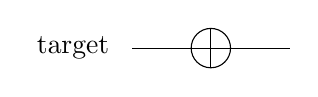
\begin{tikzpicture}[scale=.5] \node[draw=none] at (-3.5, 0) {target}; \draw (-2,0) -- (2, 0); \draw (0, 0) circle (.5); \draw (0, .5) -- (0, -.5); \end{tikzpicture} } \] ~\newline
 
\begin{DoxyParams}[1]{Parameters}
\mbox{\tt in,out}  & {\em multi\+Qubit} & object representing the set of all qubits \\
\hline
\mbox{\tt in}  & {\em target\+Qubit} & qubit to operate on \\
\hline
\end{DoxyParams}

\begin{DoxyExceptions}{Exceptions}
{\em exit\+With\+Error} & if {\ttfamily target\+Qubit} is outside \mbox{[}0, {\ttfamily multi\+Qubit.\+num\+Qubits}). \\
\hline
\end{DoxyExceptions}


Definition at line 151 of file Qu\+E\+S\+T\+\_\+env\+\_\+local.\+c.



Referenced by main(), and test\+\_\+sigma\+X().


\begin{DoxyCode}
152 \{
153     \mbox{\hyperlink{QuEST__env__local_8c_a3587b9d533e633ccf1abf9ad2ce45d8d}{QuESTAssert}}(targetQubit >= 0 && targetQubit < multiQubit.
      \mbox{\hyperlink{structMultiQubit_ab5b9795bdc6fb5855e1974dcbbaeb36f}{numQubits}}, 1, \_\_func\_\_);
154     \mbox{\hyperlink{QuEST_8c_a74822fd86bb5d81766e6e8dbdcd62df1}{sigmaXLocal}}(multiQubit, targetQubit);
155 \}
\end{DoxyCode}
\mbox{\Hypertarget{QuEST__env__local_8c_a1f54d70a42403f7e1c2e2c2007332f61}\label{QuEST__env__local_8c_a1f54d70a42403f7e1c2e2c2007332f61}} 
\index{Qu\+E\+S\+T\+\_\+env\+\_\+local.\+c@{Qu\+E\+S\+T\+\_\+env\+\_\+local.\+c}!sigmaY@{sigmaY}}
\index{sigmaY@{sigmaY}!Qu\+E\+S\+T\+\_\+env\+\_\+local.\+c@{Qu\+E\+S\+T\+\_\+env\+\_\+local.\+c}}
\paragraph{\texorpdfstring{sigma\+Y()}{sigmaY()}}
{\footnotesize\ttfamily void sigmaY (\begin{DoxyParamCaption}\item[{\mbox{\hyperlink{structMultiQubit}{Multi\+Qubit}}}]{multi\+Qubit,  }\item[{const int}]{target\+Qubit }\end{DoxyParamCaption})}



Apply the single-\/qubit sigma-\/Y (also known as the Y or Pauli-\/Y) gate. 

This is a rotation of $\pi$ around the Y-\/axis on the Bloch sphere. I.\+e. \[ \begin{pmatrix} 0 & -i \\ i & 0 \end{pmatrix} \] ~\newline
 \[ \setlength{\fboxrule}{0.01pt} \fbox{ 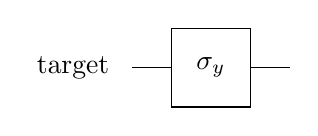
\begin{tikzpicture}[scale=.5] \node[draw=none] at (-3.5, 0) {target}; \draw (-2,0) -- (-1, 0); \draw (1, 0) -- (2, 0); \draw (-1,-1)--(-1,1)--(1,1)--(1,-1)--cycle; \node[draw=none] at (0, 0) {$\sigma_y$}; \end{tikzpicture} } \] ~\newline
 
\begin{DoxyParams}[1]{Parameters}
\mbox{\tt in,out}  & {\em multi\+Qubit} & object representing the set of all qubits \\
\hline
\mbox{\tt in}  & {\em target\+Qubit} & qubit to operate on \\
\hline
\end{DoxyParams}

\begin{DoxyExceptions}{Exceptions}
{\em exit\+With\+Error} & if {\ttfamily target\+Qubit} is outside \mbox{[}0, {\ttfamily multi\+Qubit.\+num\+Qubits}). \\
\hline
\end{DoxyExceptions}


Definition at line 157 of file Qu\+E\+S\+T\+\_\+env\+\_\+local.\+c.



Referenced by test\+\_\+sigma\+Y().


\begin{DoxyCode}
158 \{
159     \mbox{\hyperlink{QuEST__env__local_8c_a3587b9d533e633ccf1abf9ad2ce45d8d}{QuESTAssert}}(targetQubit >= 0 && targetQubit < multiQubit.
      \mbox{\hyperlink{structMultiQubit_ab5b9795bdc6fb5855e1974dcbbaeb36f}{numQubits}}, 1, \_\_func\_\_);
160     \mbox{\hyperlink{QuEST_8c_a81fbfaed65a742a7dfd622e17652245e}{sigmaYLocal}}(multiQubit, targetQubit);
161 \}
\end{DoxyCode}
\mbox{\Hypertarget{QuEST__env__local_8c_a8d31fe2d1ad4d01e2a1f5f6b8bc15b77}\label{QuEST__env__local_8c_a8d31fe2d1ad4d01e2a1f5f6b8bc15b77}} 
\index{Qu\+E\+S\+T\+\_\+env\+\_\+local.\+c@{Qu\+E\+S\+T\+\_\+env\+\_\+local.\+c}!sync\+Qu\+E\+S\+T\+Env@{sync\+Qu\+E\+S\+T\+Env}}
\index{sync\+Qu\+E\+S\+T\+Env@{sync\+Qu\+E\+S\+T\+Env}!Qu\+E\+S\+T\+\_\+env\+\_\+local.\+c@{Qu\+E\+S\+T\+\_\+env\+\_\+local.\+c}}
\paragraph{\texorpdfstring{sync\+Qu\+E\+S\+T\+Env()}{syncQuESTEnv()}}
{\footnotesize\ttfamily void sync\+Qu\+E\+S\+T\+Env (\begin{DoxyParamCaption}\item[{\mbox{\hyperlink{structQuESTEnv}{Qu\+E\+S\+T\+Env}}}]{env }\end{DoxyParamCaption})}



Guarantees that all code up to the given point has been executed on all nodes (if running in distributed mode) 


\begin{DoxyParams}[1]{Parameters}
\mbox{\tt in}  & {\em env} & object representing the execution environment. A single instance is used for each program \\
\hline
\end{DoxyParams}


Definition at line 31 of file Qu\+E\+S\+T\+\_\+env\+\_\+local.\+c.



Referenced by initialize\+State\+From\+Single\+File(), report\+State\+To\+Screen(), and test\+\_\+controlled\+Not().


\begin{DoxyCode}
31                                \{
32     \textcolor{comment}{// MPI Barrier goes here in MPI version. }
33 \} 
\end{DoxyCode}
\mbox{\Hypertarget{QuEST__env__local_8c_ac7e38d768a1bd79019f88cc1e6295092}\label{QuEST__env__local_8c_ac7e38d768a1bd79019f88cc1e6295092}} 
\index{Qu\+E\+S\+T\+\_\+env\+\_\+local.\+c@{Qu\+E\+S\+T\+\_\+env\+\_\+local.\+c}!sync\+Qu\+E\+S\+T\+Success@{sync\+Qu\+E\+S\+T\+Success}}
\index{sync\+Qu\+E\+S\+T\+Success@{sync\+Qu\+E\+S\+T\+Success}!Qu\+E\+S\+T\+\_\+env\+\_\+local.\+c@{Qu\+E\+S\+T\+\_\+env\+\_\+local.\+c}}
\paragraph{\texorpdfstring{sync\+Qu\+E\+S\+T\+Success()}{syncQuESTSuccess()}}
{\footnotesize\ttfamily int sync\+Qu\+E\+S\+T\+Success (\begin{DoxyParamCaption}\item[{int}]{success\+Code }\end{DoxyParamCaption})}



Performs a logical A\+ND on all success\+Codes held by all processes. 

If any one process has a zero success\+Code all processes will return a zero success code.


\begin{DoxyParams}[1]{Parameters}
\mbox{\tt in}  & {\em env} & object representing the execution environment. A single instance is used for each program \\
\hline
\mbox{\tt in}  & {\em success\+Code} & 1 if process task succeeded, 0 if process task failed \\
\hline
\end{DoxyParams}
\begin{DoxyReturn}{Returns}
1 if all processes succeeded, 0 if any one process failed 
\end{DoxyReturn}


Definition at line 35 of file Qu\+E\+S\+T\+\_\+env\+\_\+local.\+c.



Referenced by main().


\begin{DoxyCode}
35                                      \{
36     \textcolor{keywordflow}{return} successCode;
37 \}
\end{DoxyCode}
\mbox{\Hypertarget{QuEST__env__local_8c_a7a0877e33700f6bad48adb51b7b3fb67}\label{QuEST__env__local_8c_a7a0877e33700f6bad48adb51b7b3fb67}} 
\index{Qu\+E\+S\+T\+\_\+env\+\_\+local.\+c@{Qu\+E\+S\+T\+\_\+env\+\_\+local.\+c}!unitary@{unitary}}
\index{unitary@{unitary}!Qu\+E\+S\+T\+\_\+env\+\_\+local.\+c@{Qu\+E\+S\+T\+\_\+env\+\_\+local.\+c}}
\paragraph{\texorpdfstring{unitary()}{unitary()}}
{\footnotesize\ttfamily void unitary (\begin{DoxyParamCaption}\item[{\mbox{\hyperlink{structMultiQubit}{Multi\+Qubit}}}]{multi\+Qubit,  }\item[{const int}]{target\+Qubit,  }\item[{\mbox{\hyperlink{structComplexMatrix2}{Complex\+Matrix2}}}]{u }\end{DoxyParamCaption})}



Apply a general single-\/qubit unitary (including a global phase factor). 

The passed 2x2 Complex\+Matrix must be unitary, otherwise an error is thrown.

\[ \setlength{\fboxrule}{0.01pt} \fbox{ 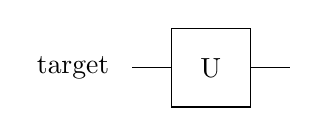
\begin{tikzpicture}[scale=.5] \node[draw=none] at (-3.5, 0) {target}; \draw (-2,0) -- (-1, 0); \draw (1, 0) -- (2, 0); \draw (-1,-1)--(-1,1)--(1,1)--(1,-1)--cycle; \node[draw=none] at (0, 0) {U}; \end{tikzpicture} } \]


\begin{DoxyParams}[1]{Parameters}
\mbox{\tt in,out}  & {\em multi\+Qubit} & object representing the set of all qubits \\
\hline
\mbox{\tt in}  & {\em target\+Qubit} & qubit to operate on \\
\hline
\mbox{\tt in}  & {\em u} & unitary matrix to apply \\
\hline
\end{DoxyParams}

\begin{DoxyExceptions}{Exceptions}
{\em exit\+With\+Error} & if {\ttfamily target\+Qubit} is outside \mbox{[}0, {\ttfamily multi\+Qubit.\+num\+Qubits}), or matrix {\ttfamily u} is not unitary. \\
\hline
\end{DoxyExceptions}


Definition at line 107 of file Qu\+E\+S\+T\+\_\+env\+\_\+local.\+c.



Referenced by main(), and test\+\_\+unitary().


\begin{DoxyCode}
108 \{
109     \mbox{\hyperlink{QuEST__env__local_8c_a3587b9d533e633ccf1abf9ad2ce45d8d}{QuESTAssert}}(targetQubit >= 0 && targetQubit < multiQubit.
      \mbox{\hyperlink{structMultiQubit_ab5b9795bdc6fb5855e1974dcbbaeb36f}{numQubits}}, 1, \_\_func\_\_);
110     \mbox{\hyperlink{QuEST__env__local_8c_a3587b9d533e633ccf1abf9ad2ce45d8d}{QuESTAssert}}(\mbox{\hyperlink{QuEST_8c_ae4fea133d1a8f09ff8da03038100adb2}{validateMatrixIsUnitary}}(u), 5, \_\_func\_\_);
111 
112     \textcolor{comment}{// all values required to update state vector lie in this rank}
113     \mbox{\hyperlink{QuEST_8c_ac134fb45b0a7248c5d15e16eb7139a35}{unitaryLocal}}(multiQubit, targetQubit, u);
114 \}
\end{DoxyCode}

\hypertarget{QuEST__env__mpi_8c}{}\subsection{Qu\+E\+S\+T\+\_\+env\+\_\+mpi.\+c File Reference}
\label{QuEST__env__mpi_8c}\index{Qu\+E\+S\+T\+\_\+env\+\_\+mpi.\+c@{Qu\+E\+S\+T\+\_\+env\+\_\+mpi.\+c}}


An implementation of the A\+PI in qubits.\+h for an M\+PI environment.  


{\ttfamily \#include \char`\"{}../\+Qu\+E\+S\+T.\+h\char`\"{}}\newline
{\ttfamily \#include \char`\"{}../\+Qu\+E\+S\+T\+\_\+precision.\+h\char`\"{}}\newline
{\ttfamily \#include \char`\"{}../mt19937ar.\+h\char`\"{}}\newline
{\ttfamily \#include \char`\"{}Qu\+E\+S\+T\+\_\+internal.\+h\char`\"{}}\newline
{\ttfamily \#include $<$unistd.\+h$>$}\newline
{\ttfamily \#include $<$mpi.\+h$>$}\newline
{\ttfamily \#include $<$stdlib.\+h$>$}\newline
{\ttfamily \#include $<$stdio.\+h$>$}\newline
{\ttfamily \#include $<$math.\+h$>$}\newline
{\ttfamily \#include $<$time.\+h$>$}\newline
{\ttfamily \#include $<$sys/types.\+h$>$}\newline
\subsubsection*{Macros}
\begin{DoxyCompactItemize}
\item 
\#define \mbox{\hyperlink{QuEST__env__mpi_8c_ad3d8a3bd0c0b677acef144f2c2ef6d73}{\+\_\+\+B\+S\+D\+\_\+\+S\+O\+U\+R\+CE}}
\end{DoxyCompactItemize}
\subsubsection*{Functions}
\begin{DoxyCompactItemize}
\item 
\mbox{\hyperlink{QuEST__precision_8h_a4b654506f18b8bfd61ad2a29a7e38c25}{R\+E\+AL}} \mbox{\hyperlink{QuEST__env__mpi_8c_a818a4c7cd7252d2b10b896b12fa431d3}{calc\+Total\+Probability}} (\mbox{\hyperlink{structMultiQubit}{Multi\+Qubit}} multi\+Qubit)
\begin{DoxyCompactList}\small\item\em Calculate the probability of being in any state by taking the norm of the entire state vector. \end{DoxyCompactList}\item 
static int \mbox{\hyperlink{QuEST__env__mpi_8c_a0552889d6f57d9e0ed8b209bf426482d}{chunk\+Is\+Upper}} (int chunk\+Id, long long int chunk\+Size, int target\+Qubit)
\begin{DoxyCompactList}\small\item\em Returns whether a given chunk in position chunk\+Id is in the upper or lower half of a block. \end{DoxyCompactList}\item 
void \mbox{\hyperlink{QuEST__env__mpi_8c_abd4bc926cd3f9b65610bb228d0c59fe0}{close\+Qu\+E\+S\+T\+Env}} (\mbox{\hyperlink{structQuESTEnv}{Qu\+E\+S\+T\+Env}} \mbox{\hyperlink{runTests_8c_a5fd8ba97fcae3408ae6221dfc3cc1f93}{env}})
\begin{DoxyCompactList}\small\item\em Close Qu\+E\+ST environment. \end{DoxyCompactList}\item 
\mbox{\hyperlink{QuEST__precision_8h_a4b654506f18b8bfd61ad2a29a7e38c25}{R\+E\+AL}} \mbox{\hyperlink{QuEST__env__mpi_8c_a07418ebac70fd9ae5d051d089961631d}{collapse\+To\+Outcome}} (\mbox{\hyperlink{structMultiQubit}{Multi\+Qubit}} multi\+Qubit, const int measure\+Qubit, int outcome)
\begin{DoxyCompactList}\small\item\em Updates the state vector to be consistent with measuring the measure qubit in the given outcome (0 or 1), and returns the probability of such a measurement outcome. \end{DoxyCompactList}\item 
void \mbox{\hyperlink{QuEST__env__mpi_8c_a03b13dfcabd8c59b50dbdd3af44ba8b2}{compact\+Unitary}} (\mbox{\hyperlink{structMultiQubit}{Multi\+Qubit}} multi\+Qubit, const int target\+Qubit, \mbox{\hyperlink{structComplex}{Complex}} alpha, \mbox{\hyperlink{structComplex}{Complex}} beta)
\begin{DoxyCompactList}\small\item\em Apply a single-\/qubit unitary parameterised by two given complex scalars. \end{DoxyCompactList}\item 
void \mbox{\hyperlink{QuEST__env__mpi_8c_ab4812953bc457405b3aa05a4c2f64f4a}{controlled\+Compact\+Unitary}} (\mbox{\hyperlink{structMultiQubit}{Multi\+Qubit}} multi\+Qubit, const int control\+Qubit, const int target\+Qubit, \mbox{\hyperlink{structComplex}{Complex}} alpha, \mbox{\hyperlink{structComplex}{Complex}} beta)
\begin{DoxyCompactList}\small\item\em Apply a controlled unitary (single control, single target) parameterised by two given complex scalars. \end{DoxyCompactList}\item 
void \mbox{\hyperlink{QuEST__env__mpi_8c_a67576895bbc65463481a8ea24d9b1e22}{controlled\+Not}} (\mbox{\hyperlink{structMultiQubit}{Multi\+Qubit}} multi\+Qubit, const int control\+Qubit, const int target\+Qubit)
\begin{DoxyCompactList}\small\item\em Apply the controlled not (single control, single target) gate, also known as the c-\/X, c-\/sigma-\/X, c-\/\+Pauli-\/X and c-\/bit-\/flip gate. \end{DoxyCompactList}\item 
void \mbox{\hyperlink{QuEST__env__mpi_8c_a8a701526263392599aa21d0d0f05d9d8}{controlled\+Unitary}} (\mbox{\hyperlink{structMultiQubit}{Multi\+Qubit}} multi\+Qubit, const int control\+Qubit, const int target\+Qubit, \mbox{\hyperlink{structComplexMatrix2}{Complex\+Matrix2}} u)
\begin{DoxyCompactList}\small\item\em Apply a general controlled unitary (single control, single target), which can include a global phase factor. \end{DoxyCompactList}\item 
void \mbox{\hyperlink{QuEST__env__mpi_8c_a7682c9a3fd592d34ec15ba8fa172f104}{exchange\+State\+Vectors}} (\mbox{\hyperlink{structMultiQubit}{Multi\+Qubit}} multi\+Qubit, int pair\+Rank)
\item 
void \mbox{\hyperlink{QuEST__env__mpi_8c_ae5f9019826f35e8b51b1716cfe397b45}{exit\+With\+Error}} (int error\+Code, const char $\ast$func)
\item 
\mbox{\hyperlink{QuEST__precision_8h_a4b654506f18b8bfd61ad2a29a7e38c25}{R\+E\+AL}} \mbox{\hyperlink{QuEST__env__mpi_8c_ad315c941a51bc053d39ebfa2040fd32e}{find\+Probability\+Of\+Outcome}} (\mbox{\hyperlink{structMultiQubit}{Multi\+Qubit}} multi\+Qubit, const int measure\+Qubit, int outcome)
\begin{DoxyCompactList}\small\item\em Gives the probability of a specified qubit being measured in the given outcome (0 or 1). \end{DoxyCompactList}\item 
static int \mbox{\hyperlink{QuEST__env__mpi_8c_a8605e6a6295174cb4661156eaa709ec4}{get\+Chunk\+Id\+From\+Index}} (\mbox{\hyperlink{structMultiQubit}{Multi\+Qubit}} multi\+Qubit, long long int index)
\item 
static int \mbox{\hyperlink{QuEST__env__mpi_8c_a7dba097f23f5d48dfdc9f3250444e2e4}{get\+Chunk\+Pair\+Id}} (int \mbox{\hyperlink{QuEST__env__mpi_8c_a0552889d6f57d9e0ed8b209bf426482d}{chunk\+Is\+Upper}}, int chunk\+Id, long long int chunk\+Size, int target\+Qubit)
\begin{DoxyCompactList}\small\item\em get position of corresponding chunk, holding values required to update values in my chunk (with chunk\+Id) when rotating target\+Qubit. \end{DoxyCompactList}\item 
\mbox{\hyperlink{QuEST__precision_8h_a4b654506f18b8bfd61ad2a29a7e38c25}{R\+E\+AL}} \mbox{\hyperlink{QuEST__env__mpi_8c_a3615f76fd5f57008d9b74bbd10533dd0}{get\+Imag\+Amp\+El}} (\mbox{\hyperlink{structMultiQubit}{Multi\+Qubit}} multi\+Qubit, long long int index)
\begin{DoxyCompactList}\small\item\em Get the imaginary component of the complex probability amplitude at an index in the state vector. \end{DoxyCompactList}\item 
\mbox{\hyperlink{QuEST__precision_8h_a4b654506f18b8bfd61ad2a29a7e38c25}{R\+E\+AL}} \mbox{\hyperlink{QuEST__env__mpi_8c_a317b786f577fa6bc136ea7f0ee7330a7}{get\+Real\+Amp\+El}} (\mbox{\hyperlink{structMultiQubit}{Multi\+Qubit}} multi\+Qubit, long long int index)
\begin{DoxyCompactList}\small\item\em Get the real component of the complex probability amplitude at an index in the state vector. \end{DoxyCompactList}\item 
static void \mbox{\hyperlink{QuEST__env__mpi_8c_adb4b0373425b282abed27742d0ce0872}{get\+Rot\+Angle}} (int \mbox{\hyperlink{QuEST__env__mpi_8c_a0552889d6f57d9e0ed8b209bf426482d}{chunk\+Is\+Upper}}, \mbox{\hyperlink{structComplex}{Complex}} $\ast$rot1, \mbox{\hyperlink{structComplex}{Complex}} $\ast$rot2, \mbox{\hyperlink{structComplex}{Complex}} alpha, \mbox{\hyperlink{structComplex}{Complex}} beta)
\begin{DoxyCompactList}\small\item\em Get rotation values for a given chunk. \end{DoxyCompactList}\item 
static void \mbox{\hyperlink{QuEST__env__mpi_8c_a5c9b2f129bdffaaba9857f6eddecbb17}{get\+Rot\+Angle\+From\+Unitary\+Matrix}} (int \mbox{\hyperlink{QuEST__env__mpi_8c_a0552889d6f57d9e0ed8b209bf426482d}{chunk\+Is\+Upper}}, \mbox{\hyperlink{structComplex}{Complex}} $\ast$rot1, \mbox{\hyperlink{structComplex}{Complex}} $\ast$rot2, \mbox{\hyperlink{structComplexMatrix2}{Complex\+Matrix2}} u)
\begin{DoxyCompactList}\small\item\em Get rotation values for a given chunk given a unitary matrix. \end{DoxyCompactList}\item 
void \mbox{\hyperlink{QuEST__env__mpi_8c_aa09b5dd93de6df1384b8f2c0041749ab}{hadamard}} (\mbox{\hyperlink{structMultiQubit}{Multi\+Qubit}} multi\+Qubit, const int target\+Qubit)
\begin{DoxyCompactList}\small\item\em Apply the single-\/qubit Hadamard gate. \end{DoxyCompactList}\item 
static int \mbox{\hyperlink{QuEST__env__mpi_8c_a4d043bb0cee54a5f94faf3ffc34a6790}{half\+Matrix\+Block\+Fits\+In\+Chunk}} (long long int chunk\+Size, int target\+Qubit)
\begin{DoxyCompactList}\small\item\em return whether the current qubit rotation will use blocks that fit within a single chunk. \end{DoxyCompactList}\item 
void \mbox{\hyperlink{QuEST__env__mpi_8c_ad84a3ce68d1ca02b4e3f741ea45b6054}{init\+Qu\+E\+S\+T\+Env}} (\mbox{\hyperlink{structQuESTEnv}{Qu\+E\+S\+T\+Env}} $\ast$\mbox{\hyperlink{runTests_8c_a5fd8ba97fcae3408ae6221dfc3cc1f93}{env}})
\begin{DoxyCompactList}\small\item\em Initialize the Qu\+E\+ST environment. \end{DoxyCompactList}\item 
static int \mbox{\hyperlink{QuEST__env__mpi_8c_af0ea25f00987af4c53f17c9cca62ab41}{is\+Chunk\+To\+Skip\+In\+Find\+P\+Zero}} (int chunk\+Id, long long int chunk\+Size, int measure\+Qubit)
\begin{DoxyCompactList}\small\item\em Find chunks to skip when calculating probability of qubit being zero. \end{DoxyCompactList}\item 
int \mbox{\hyperlink{QuEST__env__mpi_8c_ad5774247d836267175c664cd0e451bcb}{measure}} (\mbox{\hyperlink{structMultiQubit}{Multi\+Qubit}} multi\+Qubit, int measure\+Qubit)
\begin{DoxyCompactList}\small\item\em Measures a single qubit, collapsing it randomly to 0 or 1. \end{DoxyCompactList}\item 
int \mbox{\hyperlink{QuEST__env__mpi_8c_a2ac46e470c750bf93c754e06c64b0a7a}{measure\+With\+Stats}} (\mbox{\hyperlink{structMultiQubit}{Multi\+Qubit}} multi\+Qubit, int measure\+Qubit, \mbox{\hyperlink{QuEST__precision_8h_a4b654506f18b8bfd61ad2a29a7e38c25}{R\+E\+AL}} $\ast$state\+Prob)
\begin{DoxyCompactList}\small\item\em Measures a single qubit, collapsing it randomly to 0 or 1, and additionally gives the probability of that outcome. \end{DoxyCompactList}\item 
void \mbox{\hyperlink{QuEST__env__mpi_8c_ae395a79690283ed81106afadd7a8cd8a}{multi\+Controlled\+Unitary}} (\mbox{\hyperlink{structMultiQubit}{Multi\+Qubit}} multi\+Qubit, int $\ast$control\+Qubits, const int num\+Control\+Qubits, const int target\+Qubit, \mbox{\hyperlink{structComplexMatrix2}{Complex\+Matrix2}} u)
\begin{DoxyCompactList}\small\item\em Apply a general multiple-\/control single-\/target unitary, which can include a global phase factor. \end{DoxyCompactList}\item 
void \mbox{\hyperlink{QuEST__env__mpi_8c_aae7a8a7f1ccbddb7f76b6c52b746bb43}{phase\+Gate}} (\mbox{\hyperlink{structMultiQubit}{Multi\+Qubit}} multi\+Qubit, const int target\+Qubit, enum \mbox{\hyperlink{QuEST_8h_a5739021c733cecc49647956b2f7338ea}{phase\+Gate\+Type}} type)
\item 
void \mbox{\hyperlink{QuEST__env__mpi_8c_a3587b9d533e633ccf1abf9ad2ce45d8d}{Qu\+E\+S\+T\+Assert}} (int is\+Valid, int error\+Code, const char $\ast$func)
\item 
void \mbox{\hyperlink{QuEST__env__mpi_8c_a62da5b58d8ce84e6f4d24be1b872294e}{report\+Node\+List}} (\mbox{\hyperlink{structQuESTEnv}{Qu\+E\+S\+T\+Env}} \mbox{\hyperlink{runTests_8c_a5fd8ba97fcae3408ae6221dfc3cc1f93}{env}})
\begin{DoxyCompactList}\small\item\em Report a list of C\+PU hostnames and the rank that is running on each if running with M\+PI enabled and an error message otherwise. \end{DoxyCompactList}\item 
void \mbox{\hyperlink{QuEST__env__mpi_8c_af8a14ae79c3fb2c0b5f6255cc37bebf9}{report\+Qu\+E\+S\+T\+Env}} (\mbox{\hyperlink{structQuESTEnv}{Qu\+E\+S\+T\+Env}} \mbox{\hyperlink{runTests_8c_a5fd8ba97fcae3408ae6221dfc3cc1f93}{env}})
\begin{DoxyCompactList}\small\item\em Report information about the Qu\+E\+ST environment. \end{DoxyCompactList}\item 
void \mbox{\hyperlink{QuEST__env__mpi_8c_a86e396e06b7d527cac20ba0108872423}{sigmaX}} (\mbox{\hyperlink{structMultiQubit}{Multi\+Qubit}} multi\+Qubit, const int target\+Qubit)
\begin{DoxyCompactList}\small\item\em Apply the single-\/qubit sigma-\/X (also known as the X, Pauli-\/X, N\+OT or bit-\/flip) gate. \end{DoxyCompactList}\item 
void \mbox{\hyperlink{QuEST__env__mpi_8c_a1f54d70a42403f7e1c2e2c2007332f61}{sigmaY}} (\mbox{\hyperlink{structMultiQubit}{Multi\+Qubit}} multi\+Qubit, const int target\+Qubit)
\begin{DoxyCompactList}\small\item\em Apply the single-\/qubit sigma-\/Y (also known as the Y or Pauli-\/Y) gate. \end{DoxyCompactList}\item 
void \mbox{\hyperlink{QuEST__env__mpi_8c_a8d31fe2d1ad4d01e2a1f5f6b8bc15b77}{sync\+Qu\+E\+S\+T\+Env}} (\mbox{\hyperlink{structQuESTEnv}{Qu\+E\+S\+T\+Env}} \mbox{\hyperlink{runTests_8c_a5fd8ba97fcae3408ae6221dfc3cc1f93}{env}})
\begin{DoxyCompactList}\small\item\em Guarantees that all code up to the given point has been executed on all nodes (if running in distributed mode) \end{DoxyCompactList}\item 
int \mbox{\hyperlink{QuEST__env__mpi_8c_ac7e38d768a1bd79019f88cc1e6295092}{sync\+Qu\+E\+S\+T\+Success}} (int success\+Code)
\begin{DoxyCompactList}\small\item\em Performs a logical A\+ND on all success\+Codes held by all processes. \end{DoxyCompactList}\item 
void \mbox{\hyperlink{QuEST__env__mpi_8c_a7a0877e33700f6bad48adb51b7b3fb67}{unitary}} (\mbox{\hyperlink{structMultiQubit}{Multi\+Qubit}} multi\+Qubit, const int target\+Qubit, \mbox{\hyperlink{structComplexMatrix2}{Complex\+Matrix2}} u)
\begin{DoxyCompactList}\small\item\em Apply a general single-\/qubit unitary (including a global phase factor). \end{DoxyCompactList}\end{DoxyCompactItemize}


\subsubsection{Detailed Description}
An implementation of the A\+PI in qubits.\+h for an M\+PI environment. 



\subsubsection{Macro Definition Documentation}
\mbox{\Hypertarget{QuEST__env__mpi_8c_ad3d8a3bd0c0b677acef144f2c2ef6d73}\label{QuEST__env__mpi_8c_ad3d8a3bd0c0b677acef144f2c2ef6d73}} 
\index{Qu\+E\+S\+T\+\_\+env\+\_\+mpi.\+c@{Qu\+E\+S\+T\+\_\+env\+\_\+mpi.\+c}!\+\_\+\+B\+S\+D\+\_\+\+S\+O\+U\+R\+CE@{\+\_\+\+B\+S\+D\+\_\+\+S\+O\+U\+R\+CE}}
\index{\+\_\+\+B\+S\+D\+\_\+\+S\+O\+U\+R\+CE@{\+\_\+\+B\+S\+D\+\_\+\+S\+O\+U\+R\+CE}!Qu\+E\+S\+T\+\_\+env\+\_\+mpi.\+c@{Qu\+E\+S\+T\+\_\+env\+\_\+mpi.\+c}}
\paragraph{\texorpdfstring{\+\_\+\+B\+S\+D\+\_\+\+S\+O\+U\+R\+CE}{\_BSD\_SOURCE}}
{\footnotesize\ttfamily \#define \+\_\+\+B\+S\+D\+\_\+\+S\+O\+U\+R\+CE}



Definition at line 13 of file Qu\+E\+S\+T\+\_\+env\+\_\+mpi.\+c.



\subsubsection{Function Documentation}
\mbox{\Hypertarget{QuEST__env__mpi_8c_a818a4c7cd7252d2b10b896b12fa431d3}\label{QuEST__env__mpi_8c_a818a4c7cd7252d2b10b896b12fa431d3}} 
\index{Qu\+E\+S\+T\+\_\+env\+\_\+mpi.\+c@{Qu\+E\+S\+T\+\_\+env\+\_\+mpi.\+c}!calc\+Total\+Probability@{calc\+Total\+Probability}}
\index{calc\+Total\+Probability@{calc\+Total\+Probability}!Qu\+E\+S\+T\+\_\+env\+\_\+mpi.\+c@{Qu\+E\+S\+T\+\_\+env\+\_\+mpi.\+c}}
\paragraph{\texorpdfstring{calc\+Total\+Probability()}{calcTotalProbability()}}
{\footnotesize\ttfamily \mbox{\hyperlink{QuEST__precision_8h_a4b654506f18b8bfd61ad2a29a7e38c25}{R\+E\+AL}} calc\+Total\+Probability (\begin{DoxyParamCaption}\item[{\mbox{\hyperlink{structMultiQubit}{Multi\+Qubit}}}]{multi\+Qubit }\end{DoxyParamCaption})}



Calculate the probability of being in any state by taking the norm of the entire state vector. 

Should be equal to 1.


\begin{DoxyParams}[1]{Parameters}
\mbox{\tt in}  & {\em multi\+Qubit} & object representing a set of qubits \\
\hline
\end{DoxyParams}
\begin{DoxyReturn}{Returns}
total probability 
\end{DoxyReturn}


Definition at line 112 of file Qu\+E\+S\+T\+\_\+env\+\_\+mpi.\+c.



References Complex\+Array\+::imag, M\+P\+I\+\_\+\+Qu\+E\+S\+T\+\_\+\+R\+E\+AL, Multi\+Qubit\+::num\+Amps\+Per\+Chunk, Multi\+Qubit\+::num\+Chunks, Complex\+Array\+::real, R\+E\+AL, and Multi\+Qubit\+::state\+Vec.


\begin{DoxyCode}
112                                                 \{
113     \textcolor{comment}{// Implemented using Kahan summation for greater accuracy at a slight floating}
114     \textcolor{comment}{//   point operation overhead. For more details see
       https://en.wikipedia.org/wiki/Kahan\_summation\_algorithm}
115     \mbox{\hyperlink{QuEST__precision_8h_a4b654506f18b8bfd61ad2a29a7e38c25}{REAL}} pTotal=0; 
116     \mbox{\hyperlink{QuEST__precision_8h_a4b654506f18b8bfd61ad2a29a7e38c25}{REAL}} y, t, c;
117     \mbox{\hyperlink{QuEST__precision_8h_a4b654506f18b8bfd61ad2a29a7e38c25}{REAL}} allRankTotals=0;
118     \textcolor{keywordtype}{long} \textcolor{keywordtype}{long} \textcolor{keywordtype}{int} index;
119     \textcolor{keywordtype}{long} \textcolor{keywordtype}{long} \textcolor{keywordtype}{int} numAmpsPerRank = multiQubit.\mbox{\hyperlink{structMultiQubit_a1cad83601a78635dd278259c7ed54f18}{numAmpsPerChunk}};
120     c = 0.0;
121     \textcolor{keywordflow}{for} (index=0; index<numAmpsPerRank; index++)\{ 
122         \textcolor{comment}{// Perform pTotal+=multiQubit.stateVec.real[index]*multiQubit.stateVec.real[index]; by Kahan}
123         y = multiQubit.\mbox{\hyperlink{structMultiQubit_a45483190d6b01ef6b2f98f2bec9ab94f}{stateVec}}.\mbox{\hyperlink{structComplexArray_a4195cac6c784ea1b6271f1c7dba1548a}{real}}[index]*multiQubit.\mbox{\hyperlink{structMultiQubit_a45483190d6b01ef6b2f98f2bec9ab94f}{stateVec}}.
      \mbox{\hyperlink{structComplexArray_a4195cac6c784ea1b6271f1c7dba1548a}{real}}[index] - c;
124         t = pTotal + y;
125         \textcolor{comment}{// Don't change the bracketing on the following line}
126         c = ( t - pTotal ) - y;
127         pTotal = t;
128         \textcolor{comment}{// Perform pTotal+=multiQubit.stateVec.imag[index]*multiQubit.stateVec.imag[index]; by Kahan}
129         y = multiQubit.\mbox{\hyperlink{structMultiQubit_a45483190d6b01ef6b2f98f2bec9ab94f}{stateVec}}.\mbox{\hyperlink{structComplexArray_a79dde47c7ae530c79cebfdf57b225968}{imag}}[index]*multiQubit.\mbox{\hyperlink{structMultiQubit_a45483190d6b01ef6b2f98f2bec9ab94f}{stateVec}}.
      \mbox{\hyperlink{structComplexArray_a79dde47c7ae530c79cebfdf57b225968}{imag}}[index] - c;
130         t = pTotal + y;
131         \textcolor{comment}{// Don't change the bracketing on the following line}
132         c = ( t - pTotal ) - y;
133         pTotal = t;
134     \} 
135     \textcolor{keywordflow}{if} (multiQubit.\mbox{\hyperlink{structMultiQubit_acd43f2f57991709c9e94f73662c972b2}{numChunks}}>1) MPI\_Allreduce(&pTotal, &allRankTotals, 1, 
      \mbox{\hyperlink{QuEST__precision_8h_a750ad290949ef7dc4afdfbd8231a5057}{MPI\_QuEST\_REAL}}, MPI\_SUM, MPI\_COMM\_WORLD);
136     \textcolor{keywordflow}{else} allRankTotals=pTotal;
137 
138     \textcolor{keywordflow}{return} allRankTotals;
139 \}
\end{DoxyCode}
\mbox{\Hypertarget{QuEST__env__mpi_8c_a0552889d6f57d9e0ed8b209bf426482d}\label{QuEST__env__mpi_8c_a0552889d6f57d9e0ed8b209bf426482d}} 
\index{Qu\+E\+S\+T\+\_\+env\+\_\+mpi.\+c@{Qu\+E\+S\+T\+\_\+env\+\_\+mpi.\+c}!chunk\+Is\+Upper@{chunk\+Is\+Upper}}
\index{chunk\+Is\+Upper@{chunk\+Is\+Upper}!Qu\+E\+S\+T\+\_\+env\+\_\+mpi.\+c@{Qu\+E\+S\+T\+\_\+env\+\_\+mpi.\+c}}
\paragraph{\texorpdfstring{chunk\+Is\+Upper()}{chunkIsUpper()}}
{\footnotesize\ttfamily static int chunk\+Is\+Upper (\begin{DoxyParamCaption}\item[{int}]{chunk\+Id,  }\item[{long long int}]{chunk\+Size,  }\item[{int}]{target\+Qubit }\end{DoxyParamCaption})\hspace{0.3cm}{\ttfamily [static]}}



Returns whether a given chunk in position chunk\+Id is in the upper or lower half of a block. 


\begin{DoxyParams}[1]{Parameters}
\mbox{\tt in}  & {\em chunk\+Id} & id of chunk in state vector \\
\hline
\mbox{\tt in}  & {\em chunk\+Size} & number of amps in chunk \\
\hline
\mbox{\tt in}  & {\em target\+Qubit} & qubit being rotated \\
\hline
\end{DoxyParams}
\begin{DoxyReturn}{Returns}
1\+: chunk is in upper half of block, 0\+: chunk is in lower half of block fix -- is this the same as is\+Chunk\+To\+Skip? 
\end{DoxyReturn}


Definition at line 150 of file Qu\+E\+S\+T\+\_\+env\+\_\+mpi.\+c.



Referenced by compact\+Unitary(), controlled\+Compact\+Unitary(), controlled\+Not(), controlled\+Unitary(), get\+Chunk\+Pair\+Id(), get\+Rot\+Angle(), get\+Rot\+Angle\+From\+Unitary\+Matrix(), hadamard(), multi\+Controlled\+Unitary(), phase\+Gate(), sigma\+X(), sigma\+Y(), and unitary().


\begin{DoxyCode}
151 \{       
152     \textcolor{keywordtype}{long} \textcolor{keywordtype}{long} \textcolor{keywordtype}{int} sizeHalfBlock = 1LL << (targetQubit);
153     \textcolor{keywordtype}{long} \textcolor{keywordtype}{long} \textcolor{keywordtype}{int} sizeBlock = sizeHalfBlock*2;
154     \textcolor{keywordtype}{long} \textcolor{keywordtype}{long} \textcolor{keywordtype}{int} posInBlock = (chunkId*chunkSize) % sizeBlock;
155     \textcolor{keywordflow}{return} posInBlock<sizeHalfBlock;
156 \}
\end{DoxyCode}
\mbox{\Hypertarget{QuEST__env__mpi_8c_abd4bc926cd3f9b65610bb228d0c59fe0}\label{QuEST__env__mpi_8c_abd4bc926cd3f9b65610bb228d0c59fe0}} 
\index{Qu\+E\+S\+T\+\_\+env\+\_\+mpi.\+c@{Qu\+E\+S\+T\+\_\+env\+\_\+mpi.\+c}!close\+Qu\+E\+S\+T\+Env@{close\+Qu\+E\+S\+T\+Env}}
\index{close\+Qu\+E\+S\+T\+Env@{close\+Qu\+E\+S\+T\+Env}!Qu\+E\+S\+T\+\_\+env\+\_\+mpi.\+c@{Qu\+E\+S\+T\+\_\+env\+\_\+mpi.\+c}}
\paragraph{\texorpdfstring{close\+Qu\+E\+S\+T\+Env()}{closeQuESTEnv()}}
{\footnotesize\ttfamily void close\+Qu\+E\+S\+T\+Env (\begin{DoxyParamCaption}\item[{\mbox{\hyperlink{structQuESTEnv}{Qu\+E\+S\+T\+Env}}}]{env }\end{DoxyParamCaption})}



Close Qu\+E\+ST environment. 

If something needs to be done to clean up the execution environment, such as finalizing M\+PI when running in distributed mode, it is handled here


\begin{DoxyParams}[1]{Parameters}
\mbox{\tt in}  & {\em env} & object representing the execution environment. A single instance is used for each program \\
\hline
\end{DoxyParams}


Definition at line 60 of file Qu\+E\+S\+T\+\_\+env\+\_\+mpi.\+c.


\begin{DoxyCode}
60                                 \{
61     \textcolor{keywordtype}{int} finalized;
62     MPI\_Finalized(&finalized);
63     \textcolor{keywordflow}{if} (!finalized) MPI\_Finalize();
64     \textcolor{keywordflow}{else} printf(\textcolor{stringliteral}{"ERROR: Trying to close QuESTEnv multiple times. Ignoring\(\backslash\)n"});
65 \}
\end{DoxyCode}
\mbox{\Hypertarget{QuEST__env__mpi_8c_a07418ebac70fd9ae5d051d089961631d}\label{QuEST__env__mpi_8c_a07418ebac70fd9ae5d051d089961631d}} 
\index{Qu\+E\+S\+T\+\_\+env\+\_\+mpi.\+c@{Qu\+E\+S\+T\+\_\+env\+\_\+mpi.\+c}!collapse\+To\+Outcome@{collapse\+To\+Outcome}}
\index{collapse\+To\+Outcome@{collapse\+To\+Outcome}!Qu\+E\+S\+T\+\_\+env\+\_\+mpi.\+c@{Qu\+E\+S\+T\+\_\+env\+\_\+mpi.\+c}}
\paragraph{\texorpdfstring{collapse\+To\+Outcome()}{collapseToOutcome()}}
{\footnotesize\ttfamily \mbox{\hyperlink{QuEST__precision_8h_a4b654506f18b8bfd61ad2a29a7e38c25}{R\+E\+AL}} collapse\+To\+Outcome (\begin{DoxyParamCaption}\item[{\mbox{\hyperlink{structMultiQubit}{Multi\+Qubit}}}]{multi\+Qubit,  }\item[{const int}]{measure\+Qubit,  }\item[{int}]{outcome }\end{DoxyParamCaption})}



Updates the state vector to be consistent with measuring the measure qubit in the given outcome (0 or 1), and returns the probability of such a measurement outcome. 

This is effectively performing a measurement and forcing the outcome. This is an irreversible change to the state vector, whereby incompatible states in the state vector are given zero amplitude and the remaining states are renormalised. Exits with error if the given outcome has $\sim$zero probability, and so cannot be collapsed into.


\begin{DoxyParams}[1]{Parameters}
\mbox{\tt in,out}  & {\em multi\+Qubit} & object representing the set of all qubits \\
\hline
\mbox{\tt in}  & {\em measure\+Qubit} & qubit to measure \\
\hline
\mbox{\tt in}  & {\em outcome} & to force the measure qubit to enter \\
\hline
\end{DoxyParams}
\begin{DoxyReturn}{Returns}
probability of the (forced) measurement outcome 
\end{DoxyReturn}

\begin{DoxyExceptions}{Exceptions}
{\em exit\+With\+Error} & if {\ttfamily measure\+Qubit} is outside \mbox{[}0, {\ttfamily multi\+Qubit.\+num\+Qubits}), or if {\ttfamily outcome} is not in \{0, 1\}, or if the probability of {\ttfamily outcome} is zero (within machine epsilon) \\
\hline
\end{DoxyExceptions}


Definition at line 678 of file Qu\+E\+S\+T\+\_\+env\+\_\+mpi.\+c.



References Multi\+Qubit\+::chunk\+Id, collapse\+To\+Outcome\+Distributed\+Renorm(), collapse\+To\+Outcome\+Distributed\+Set\+Zero(), collapse\+To\+Outcome\+Local(), find\+Probability\+Of\+Outcome(), half\+Matrix\+Block\+Fits\+In\+Chunk(), is\+Chunk\+To\+Skip\+In\+Find\+P\+Zero(), Multi\+Qubit\+::num\+Amps\+Per\+Chunk, Multi\+Qubit\+::num\+Qubits, Qu\+E\+S\+T\+Assert(), R\+E\+AL, and R\+E\+A\+L\+\_\+\+E\+PS.


\begin{DoxyCode}
679 \{
680     \mbox{\hyperlink{QuEST__env__mpi_8c_a3587b9d533e633ccf1abf9ad2ce45d8d}{QuESTAssert}}(measureQubit >= 0 && measureQubit < multiQubit.
      \mbox{\hyperlink{structMultiQubit_ab5b9795bdc6fb5855e1974dcbbaeb36f}{numQubits}}, 2, \_\_func\_\_);
681     \mbox{\hyperlink{QuEST__env__mpi_8c_a3587b9d533e633ccf1abf9ad2ce45d8d}{QuESTAssert}}((outcome==0 || outcome==1), 10, \_\_func\_\_);
682 
683     \mbox{\hyperlink{QuEST__precision_8h_a4b654506f18b8bfd61ad2a29a7e38c25}{REAL}} totalStateProb=\mbox{\hyperlink{QuEST__env__mpi_8c_ad315c941a51bc053d39ebfa2040fd32e}{findProbabilityOfOutcome}}(multiQubit, measureQubit, 
      outcome);
684     \mbox{\hyperlink{QuEST__env__mpi_8c_a3587b9d533e633ccf1abf9ad2ce45d8d}{QuESTAssert}}(fabs(totalStateProb)>\mbox{\hyperlink{QuEST__precision_8h_aebb5e6716e06431296af4d1a71744dec}{REAL\_EPS}}, 8, \_\_func\_\_);
685 
686     \textcolor{keywordtype}{int} skipValuesWithinRank = \mbox{\hyperlink{QuEST__env__mpi_8c_a4d043bb0cee54a5f94faf3ffc34a6790}{halfMatrixBlockFitsInChunk}}(multiQubit.
      \mbox{\hyperlink{structMultiQubit_a1cad83601a78635dd278259c7ed54f18}{numAmpsPerChunk}}, measureQubit);
687     \textcolor{keywordflow}{if} (skipValuesWithinRank) \{
688         \mbox{\hyperlink{QuEST_8c_a01d9a8b7ff0e09ec399e158389783aa9}{collapseToOutcomeLocal}}(multiQubit, measureQubit, totalStateProb, outcome);
689     \} \textcolor{keywordflow}{else} \{
690         \textcolor{keywordflow}{if} (!\mbox{\hyperlink{QuEST__env__mpi_8c_af0ea25f00987af4c53f17c9cca62ab41}{isChunkToSkipInFindPZero}}(multiQubit.\mbox{\hyperlink{structMultiQubit_ab10c88249fa3825d6227ceec01d37e37}{chunkId}}, multiQubit.
      \mbox{\hyperlink{structMultiQubit_a1cad83601a78635dd278259c7ed54f18}{numAmpsPerChunk}}, measureQubit))\{
691             \textcolor{comment}{// chunk has amps for q=0}
692             \textcolor{keywordflow}{if} (outcome==0) \mbox{\hyperlink{QuEST_8c_a7a1f63ec3c42d9ad72f1f01c14a885db}{collapseToOutcomeDistributedRenorm}}(multiQubit
      , measureQubit, 
693                     totalStateProb);
694             \textcolor{keywordflow}{else} \mbox{\hyperlink{QuEST_8c_a78908fe8e75a21fd4f7fa7dff05d6be1}{collapseToOutcomeDistributedSetZero}}(multiQubit, 
      measureQubit);
695         \} \textcolor{keywordflow}{else} \{
696             \textcolor{comment}{// chunk has amps for q=1}
697             \textcolor{keywordflow}{if} (outcome==1) \mbox{\hyperlink{QuEST_8c_a7a1f63ec3c42d9ad72f1f01c14a885db}{collapseToOutcomeDistributedRenorm}}(multiQubit
      , measureQubit, 
698                     totalStateProb);
699             \textcolor{keywordflow}{else} \mbox{\hyperlink{QuEST_8c_a78908fe8e75a21fd4f7fa7dff05d6be1}{collapseToOutcomeDistributedSetZero}}(multiQubit, 
      measureQubit);
700         \}
701     \}
702     \textcolor{keywordflow}{return} totalStateProb;
703 \}
\end{DoxyCode}
\mbox{\Hypertarget{QuEST__env__mpi_8c_a03b13dfcabd8c59b50dbdd3af44ba8b2}\label{QuEST__env__mpi_8c_a03b13dfcabd8c59b50dbdd3af44ba8b2}} 
\index{Qu\+E\+S\+T\+\_\+env\+\_\+mpi.\+c@{Qu\+E\+S\+T\+\_\+env\+\_\+mpi.\+c}!compact\+Unitary@{compact\+Unitary}}
\index{compact\+Unitary@{compact\+Unitary}!Qu\+E\+S\+T\+\_\+env\+\_\+mpi.\+c@{Qu\+E\+S\+T\+\_\+env\+\_\+mpi.\+c}}
\paragraph{\texorpdfstring{compact\+Unitary()}{compactUnitary()}}
{\footnotesize\ttfamily void compact\+Unitary (\begin{DoxyParamCaption}\item[{\mbox{\hyperlink{structMultiQubit}{Multi\+Qubit}}}]{multi\+Qubit,  }\item[{const int}]{target\+Qubit,  }\item[{\mbox{\hyperlink{structComplex}{Complex}}}]{alpha,  }\item[{\mbox{\hyperlink{structComplex}{Complex}}}]{beta }\end{DoxyParamCaption})}



Apply a single-\/qubit unitary parameterised by two given complex scalars. 

Given valid complex numbers $\alpha$ and $\beta$, applies the unitary \[ U = \begin{pmatrix} \alpha & -\beta^* \\ \beta & \alpha^* \end{pmatrix} \] which is general up to a global phase factor. ~\newline
Valid $\alpha$, $\beta$ satisfy $|\alpha|^2 + |\beta|^2 = 1$.

\[ \setlength{\fboxrule}{0.01pt} \fbox{ 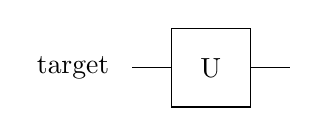
\begin{tikzpicture}[scale=.5] \node[draw=none] at (-3.5, 0) {target}; \draw (-2,0) -- (-1, 0); \draw (1, 0) -- (2, 0); \draw (-1,-1)--(-1,1)--(1,1)--(1,-1)--cycle; \node[draw=none] at (0, 0) {U}; \end{tikzpicture} } \]


\begin{DoxyParams}[1]{Parameters}
\mbox{\tt in,out}  & {\em multi\+Qubit} & object representing the set of all qubits \\
\hline
\mbox{\tt in}  & {\em target\+Qubit} & qubit to operate on \\
\hline
\mbox{\tt in}  & {\em alpha} & complex unitary parameter (row 1, column 1) \\
\hline
\mbox{\tt in}  & {\em beta} & complex unitary parameter (row 2, column 1) \\
\hline
\end{DoxyParams}

\begin{DoxyExceptions}{Exceptions}
{\em exit\+With\+Error} & if {\ttfamily target\+Qubit} is outside \mbox{[}0, {\ttfamily multi\+Qubit.\+num\+Qubits}), or if {\ttfamily alpha}, {\ttfamily beta} don\textquotesingle{}t satisfy $\vert${\ttfamily alpha$\vert$$^\wedge$2} + $\vert${\ttfamily beta$\vert$$^\wedge$2} = 1. \\
\hline
\end{DoxyExceptions}


Definition at line 272 of file Qu\+E\+S\+T\+\_\+env\+\_\+mpi.\+c.



References Multi\+Qubit\+::chunk\+Id, chunk\+Is\+Upper(), compact\+Unitary\+Distributed(), compact\+Unitary\+Local(), exchange\+State\+Vectors(), get\+Chunk\+Pair\+Id(), get\+Rot\+Angle(), half\+Matrix\+Block\+Fits\+In\+Chunk(), Multi\+Qubit\+::num\+Amps\+Per\+Chunk, Multi\+Qubit\+::num\+Qubits, Multi\+Qubit\+::pair\+State\+Vec, Qu\+E\+S\+T\+Assert(), Multi\+Qubit\+::state\+Vec, and validate\+Alpha\+Beta().


\begin{DoxyCode}
273 \{
274     \mbox{\hyperlink{QuEST__env__mpi_8c_a3587b9d533e633ccf1abf9ad2ce45d8d}{QuESTAssert}}(targetQubit >= 0 && targetQubit < multiQubit.
      \mbox{\hyperlink{structMultiQubit_ab5b9795bdc6fb5855e1974dcbbaeb36f}{numQubits}}, 1, \_\_func\_\_);
275     \mbox{\hyperlink{QuEST__env__mpi_8c_a3587b9d533e633ccf1abf9ad2ce45d8d}{QuESTAssert}}(\mbox{\hyperlink{QuEST_8c_ae2b2c14a07dd7d50ff86032a3ca101d7}{validateAlphaBeta}}(alpha, beta), 6, \_\_func\_\_);
276 
277     \textcolor{comment}{// flag to require memory exchange. 1: an entire block fits on one rank, 0: at most half a block fits
       on one rank}
278     \textcolor{keywordtype}{int} useLocalDataOnly = \mbox{\hyperlink{QuEST__env__mpi_8c_a4d043bb0cee54a5f94faf3ffc34a6790}{halfMatrixBlockFitsInChunk}}(multiQubit.
      \mbox{\hyperlink{structMultiQubit_a1cad83601a78635dd278259c7ed54f18}{numAmpsPerChunk}}, targetQubit);
279     \mbox{\hyperlink{structComplex}{Complex}} rot1, rot2;
280 
281     \textcolor{comment}{// rank's chunk is in upper half of block }
282     \textcolor{keywordtype}{int} rankIsUpper;
283     \textcolor{keywordtype}{int} pairRank; \textcolor{comment}{// rank of corresponding chunk}
284 
285     \textcolor{keywordflow}{if} (useLocalDataOnly)\{
286         \textcolor{comment}{// all values required to update state vector lie in this rank}
287         \mbox{\hyperlink{QuEST_8c_a9cee2d8716667a3318420a3b672f5b92}{compactUnitaryLocal}}(multiQubit, targetQubit, alpha, beta);
288     \} \textcolor{keywordflow}{else} \{
289         \textcolor{comment}{// need to get corresponding chunk of state vector from other rank}
290         rankIsUpper = \mbox{\hyperlink{QuEST__env__mpi_8c_a0552889d6f57d9e0ed8b209bf426482d}{chunkIsUpper}}(multiQubit.\mbox{\hyperlink{structMultiQubit_ab10c88249fa3825d6227ceec01d37e37}{chunkId}}, multiQubit.
      \mbox{\hyperlink{structMultiQubit_a1cad83601a78635dd278259c7ed54f18}{numAmpsPerChunk}}, targetQubit);
291         \mbox{\hyperlink{QuEST__env__mpi_8c_adb4b0373425b282abed27742d0ce0872}{getRotAngle}}(rankIsUpper, &rot1, &rot2, alpha, beta);
292         pairRank = \mbox{\hyperlink{QuEST__env__mpi_8c_a7dba097f23f5d48dfdc9f3250444e2e4}{getChunkPairId}}(rankIsUpper, multiQubit.\mbox{\hyperlink{structMultiQubit_ab10c88249fa3825d6227ceec01d37e37}{chunkId}}, multiQubit.
      \mbox{\hyperlink{structMultiQubit_a1cad83601a78635dd278259c7ed54f18}{numAmpsPerChunk}}, targetQubit);
293         \textcolor{comment}{// get corresponding values from my pair}
294         \mbox{\hyperlink{QuEST__env__mpi_8c_a7682c9a3fd592d34ec15ba8fa172f104}{exchangeStateVectors}}(multiQubit, pairRank);
295 
296         \textcolor{comment}{// this rank's values are either in the upper of lower half of the block. }
297         \textcolor{comment}{// send values to compactUnitaryDistributed in the correct order}
298         \textcolor{keywordflow}{if} (rankIsUpper)\{
299             \mbox{\hyperlink{QuEST_8c_a20ee1878a63ae6112e8845f4a8787592}{compactUnitaryDistributed}}(multiQubit,targetQubit,rot1,rot2,
300                     multiQubit.\mbox{\hyperlink{structMultiQubit_a45483190d6b01ef6b2f98f2bec9ab94f}{stateVec}}, \textcolor{comment}{//upper}
301                     multiQubit.\mbox{\hyperlink{structMultiQubit_a76f7db4eab52d2b30f58f973ada809c5}{pairStateVec}}, \textcolor{comment}{//lower}
302                     multiQubit.\mbox{\hyperlink{structMultiQubit_a45483190d6b01ef6b2f98f2bec9ab94f}{stateVec}}); \textcolor{comment}{//output}
303         \} \textcolor{keywordflow}{else} \{
304             \mbox{\hyperlink{QuEST_8c_a20ee1878a63ae6112e8845f4a8787592}{compactUnitaryDistributed}}(multiQubit,targetQubit,rot1,rot2,
305                     multiQubit.\mbox{\hyperlink{structMultiQubit_a76f7db4eab52d2b30f58f973ada809c5}{pairStateVec}}, \textcolor{comment}{//upper}
306                     multiQubit.\mbox{\hyperlink{structMultiQubit_a45483190d6b01ef6b2f98f2bec9ab94f}{stateVec}}, \textcolor{comment}{//lower}
307                     multiQubit.\mbox{\hyperlink{structMultiQubit_a45483190d6b01ef6b2f98f2bec9ab94f}{stateVec}}); \textcolor{comment}{//output}
308         \}
309     \}
310 \}
\end{DoxyCode}
\mbox{\Hypertarget{QuEST__env__mpi_8c_ab4812953bc457405b3aa05a4c2f64f4a}\label{QuEST__env__mpi_8c_ab4812953bc457405b3aa05a4c2f64f4a}} 
\index{Qu\+E\+S\+T\+\_\+env\+\_\+mpi.\+c@{Qu\+E\+S\+T\+\_\+env\+\_\+mpi.\+c}!controlled\+Compact\+Unitary@{controlled\+Compact\+Unitary}}
\index{controlled\+Compact\+Unitary@{controlled\+Compact\+Unitary}!Qu\+E\+S\+T\+\_\+env\+\_\+mpi.\+c@{Qu\+E\+S\+T\+\_\+env\+\_\+mpi.\+c}}
\paragraph{\texorpdfstring{controlled\+Compact\+Unitary()}{controlledCompactUnitary()}}
{\footnotesize\ttfamily void controlled\+Compact\+Unitary (\begin{DoxyParamCaption}\item[{\mbox{\hyperlink{structMultiQubit}{Multi\+Qubit}}}]{multi\+Qubit,  }\item[{const int}]{control\+Qubit,  }\item[{const int}]{target\+Qubit,  }\item[{\mbox{\hyperlink{structComplex}{Complex}}}]{alpha,  }\item[{\mbox{\hyperlink{structComplex}{Complex}}}]{beta }\end{DoxyParamCaption})}



Apply a controlled unitary (single control, single target) parameterised by two given complex scalars. 

Given valid complex numbers $\alpha$ and $\beta$, applies the two-\/qubit unitary \[ \begin{pmatrix} 1 \\ & 1 \\ & & \alpha & -\beta^* \\ & & \beta & \alpha^* \end{pmatrix} \] to the control and target qubits. Valid $\alpha$, $\beta$ satisfy $|\alpha|^2 + |\beta|^2 = 1$. The target unitary is general up to a global phase factor. ~\newline
 \[ \setlength{\fboxrule}{0.01pt} \fbox{ 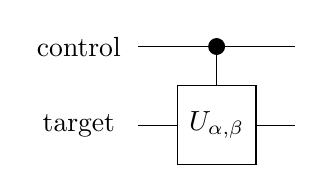
\begin{tikzpicture}[scale=.5] \node[draw=none] at (-3.5, 2) {control}; \node[draw=none] at (-3.5, 0) {target}; \draw (-2, 2) -- (2, 2); \draw[fill=black] (0, 2) circle (.2); \draw (0, 2) -- (0, 1); \draw (-2,0) -- (-1, 0); \draw (1, 0) -- (2, 0); \draw (-1,-1)--(-1,1)--(1,1)--(1,-1)--cycle; \node[draw=none] at (0, 0) {$U_{\alpha, \beta}$}; \end{tikzpicture} } \]


\begin{DoxyParams}[1]{Parameters}
\mbox{\tt in,out}  & {\em multi\+Qubit} & object representing the set of all qubits \\
\hline
\mbox{\tt in}  & {\em control\+Qubit} & apply the target unitary if this qubit has value 1 \\
\hline
\mbox{\tt in}  & {\em target\+Qubit} & qubit on which to apply the target unitary \\
\hline
\mbox{\tt in}  & {\em alpha} & complex unitary parameter (row 1, column 1) \\
\hline
\mbox{\tt in}  & {\em beta} & complex unitary parameter (row 2, column 1) \\
\hline
\end{DoxyParams}

\begin{DoxyExceptions}{Exceptions}
{\em exit\+With\+Error} & if either {\ttfamily control\+Qubit} or {\ttfamily target\+Qubit} are outside \mbox{[}0, {\ttfamily multi\+Qubit.\+num\+Qubits}) or are equal, or if {\ttfamily alpha}, {\ttfamily beta} don\textquotesingle{}t satisfy $\vert${\ttfamily alpha$\vert$$^\wedge$2} + $\vert${\ttfamily beta$\vert$$^\wedge$2} = 1. \\
\hline
\end{DoxyExceptions}


Definition at line 354 of file Qu\+E\+S\+T\+\_\+env\+\_\+mpi.\+c.



References Multi\+Qubit\+::chunk\+Id, chunk\+Is\+Upper(), controlled\+Compact\+Unitary\+Distributed(), controlled\+Compact\+Unitary\+Local(), exchange\+State\+Vectors(), get\+Chunk\+Pair\+Id(), get\+Rot\+Angle(), half\+Matrix\+Block\+Fits\+In\+Chunk(), Multi\+Qubit\+::num\+Amps\+Per\+Chunk, Multi\+Qubit\+::num\+Qubits, Multi\+Qubit\+::pair\+State\+Vec, Qu\+E\+S\+T\+Assert(), Multi\+Qubit\+::state\+Vec, and validate\+Alpha\+Beta().


\begin{DoxyCode}
355 \{
356     \mbox{\hyperlink{QuEST__env__mpi_8c_a3587b9d533e633ccf1abf9ad2ce45d8d}{QuESTAssert}}(targetQubit >= 0 && targetQubit < multiQubit.
      \mbox{\hyperlink{structMultiQubit_ab5b9795bdc6fb5855e1974dcbbaeb36f}{numQubits}}, 1, \_\_func\_\_);
357     \mbox{\hyperlink{QuEST__env__mpi_8c_a3587b9d533e633ccf1abf9ad2ce45d8d}{QuESTAssert}}(controlQubit >= 0 && controlQubit < multiQubit.
      \mbox{\hyperlink{structMultiQubit_ab5b9795bdc6fb5855e1974dcbbaeb36f}{numQubits}}, 2, \_\_func\_\_);
358     \mbox{\hyperlink{QuEST__env__mpi_8c_a3587b9d533e633ccf1abf9ad2ce45d8d}{QuESTAssert}}(controlQubit != targetQubit, 3, \_\_func\_\_);
359     \mbox{\hyperlink{QuEST__env__mpi_8c_a3587b9d533e633ccf1abf9ad2ce45d8d}{QuESTAssert}}(\mbox{\hyperlink{QuEST_8c_ae2b2c14a07dd7d50ff86032a3ca101d7}{validateAlphaBeta}}(alpha, beta), 6, \_\_func\_\_);
360 
361     \textcolor{comment}{// flag to require memory exchange. 1: an entire block fits on one rank, 0: at most half a block fits
       on one rank}
362     \textcolor{keywordtype}{int} useLocalDataOnly = \mbox{\hyperlink{QuEST__env__mpi_8c_a4d043bb0cee54a5f94faf3ffc34a6790}{halfMatrixBlockFitsInChunk}}(multiQubit.
      \mbox{\hyperlink{structMultiQubit_a1cad83601a78635dd278259c7ed54f18}{numAmpsPerChunk}}, targetQubit);
363     \mbox{\hyperlink{structComplex}{Complex}} rot1, rot2;
364 
365     \textcolor{comment}{// rank's chunk is in upper half of block }
366     \textcolor{keywordtype}{int} rankIsUpper;
367     \textcolor{keywordtype}{int} pairRank; \textcolor{comment}{// rank of corresponding chunk}
368 
369     \textcolor{keywordflow}{if} (useLocalDataOnly)\{
370         \textcolor{comment}{// all values required to update state vector lie in this rank}
371         \mbox{\hyperlink{QuEST_8c_afc77657651d52c47403b44b923a098a8}{controlledCompactUnitaryLocal}}(multiQubit, controlQubit, targetQubit, 
      alpha, beta);
372     \} \textcolor{keywordflow}{else} \{
373         \textcolor{comment}{// need to get corresponding chunk of state vector from other rank}
374         rankIsUpper = \mbox{\hyperlink{QuEST__env__mpi_8c_a0552889d6f57d9e0ed8b209bf426482d}{chunkIsUpper}}(multiQubit.\mbox{\hyperlink{structMultiQubit_ab10c88249fa3825d6227ceec01d37e37}{chunkId}}, multiQubit.
      \mbox{\hyperlink{structMultiQubit_a1cad83601a78635dd278259c7ed54f18}{numAmpsPerChunk}}, targetQubit);
375         \mbox{\hyperlink{QuEST__env__mpi_8c_adb4b0373425b282abed27742d0ce0872}{getRotAngle}}(rankIsUpper, &rot1, &rot2, alpha, beta);
376         pairRank = \mbox{\hyperlink{QuEST__env__mpi_8c_a7dba097f23f5d48dfdc9f3250444e2e4}{getChunkPairId}}(rankIsUpper, multiQubit.\mbox{\hyperlink{structMultiQubit_ab10c88249fa3825d6227ceec01d37e37}{chunkId}}, multiQubit.
      \mbox{\hyperlink{structMultiQubit_a1cad83601a78635dd278259c7ed54f18}{numAmpsPerChunk}}, targetQubit);
377         \textcolor{comment}{//printf("%d rank has pair rank: %d\(\backslash\)n", multiQubit.rank, pairRank);}
378         \textcolor{comment}{// get corresponding values from my pair}
379         \mbox{\hyperlink{QuEST__env__mpi_8c_a7682c9a3fd592d34ec15ba8fa172f104}{exchangeStateVectors}}(multiQubit, pairRank);
380 
381         \textcolor{comment}{// this rank's values are either in the upper of lower half of the block. send values to
       controlledCompactUnitaryDistributed}
382         \textcolor{comment}{// in the correct order}
383         \textcolor{keywordflow}{if} (rankIsUpper)\{
384             \mbox{\hyperlink{QuEST_8c_a717855e835e3161e08c18cdc15325d27}{controlledCompactUnitaryDistributed}}(multiQubit,controlQubit,
      targetQubit,rot1,rot2,
385                     multiQubit.\mbox{\hyperlink{structMultiQubit_a45483190d6b01ef6b2f98f2bec9ab94f}{stateVec}}, \textcolor{comment}{//upper}
386                     multiQubit.\mbox{\hyperlink{structMultiQubit_a76f7db4eab52d2b30f58f973ada809c5}{pairStateVec}}, \textcolor{comment}{//lower}
387                     multiQubit.\mbox{\hyperlink{structMultiQubit_a45483190d6b01ef6b2f98f2bec9ab94f}{stateVec}}); \textcolor{comment}{//output}
388         \} \textcolor{keywordflow}{else} \{
389             \mbox{\hyperlink{QuEST_8c_a717855e835e3161e08c18cdc15325d27}{controlledCompactUnitaryDistributed}}(multiQubit,controlQubit,
      targetQubit,rot1,rot2,
390                     multiQubit.\mbox{\hyperlink{structMultiQubit_a76f7db4eab52d2b30f58f973ada809c5}{pairStateVec}}, \textcolor{comment}{//upper}
391                     multiQubit.\mbox{\hyperlink{structMultiQubit_a45483190d6b01ef6b2f98f2bec9ab94f}{stateVec}}, \textcolor{comment}{//lower}
392                     multiQubit.\mbox{\hyperlink{structMultiQubit_a45483190d6b01ef6b2f98f2bec9ab94f}{stateVec}}); \textcolor{comment}{//output}
393         \}
394     \}
395 \}
\end{DoxyCode}
\mbox{\Hypertarget{QuEST__env__mpi_8c_a67576895bbc65463481a8ea24d9b1e22}\label{QuEST__env__mpi_8c_a67576895bbc65463481a8ea24d9b1e22}} 
\index{Qu\+E\+S\+T\+\_\+env\+\_\+mpi.\+c@{Qu\+E\+S\+T\+\_\+env\+\_\+mpi.\+c}!controlled\+Not@{controlled\+Not}}
\index{controlled\+Not@{controlled\+Not}!Qu\+E\+S\+T\+\_\+env\+\_\+mpi.\+c@{Qu\+E\+S\+T\+\_\+env\+\_\+mpi.\+c}}
\paragraph{\texorpdfstring{controlled\+Not()}{controlledNot()}}
{\footnotesize\ttfamily void controlled\+Not (\begin{DoxyParamCaption}\item[{\mbox{\hyperlink{structMultiQubit}{Multi\+Qubit}}}]{multi\+Qubit,  }\item[{const int}]{control\+Qubit,  }\item[{const int}]{target\+Qubit }\end{DoxyParamCaption})}



Apply the controlled not (single control, single target) gate, also known as the c-\/X, c-\/sigma-\/X, c-\/\+Pauli-\/X and c-\/bit-\/flip gate. 

This applies sigmaX to the target qubit if the control qubit has value 1. This effects the two-\/qubit unitary \[ \begin{pmatrix} 1 \\ & 1 \\\ & & & 1 \\ & & 1 \end{pmatrix} \] on the control and target qubits.

\[ \setlength{\fboxrule}{0.01pt} \fbox{ 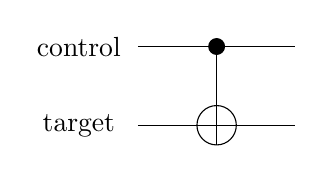
\begin{tikzpicture}[scale=.5] \node[draw=none] at (-3.5, 2) {control}; \node[draw=none] at (-3.5, 0) {target}; \draw (-2, 2) -- (2, 2); \draw[fill=black] (0, 2) circle (.2); \draw (0, 2) -- (0, -.5); \draw (-2,0) -- (2, 0); \draw (0, 0) circle (.5); \end{tikzpicture} } \] ~\newline
 
\begin{DoxyParams}[1]{Parameters}
\mbox{\tt in,out}  & {\em multi\+Qubit} & object representing the set of all qubits \\
\hline
\mbox{\tt in}  & {\em control\+Qubit} & nots the target if this qubit is 1 \\
\hline
\mbox{\tt in}  & {\em target\+Qubit} & qubit to not \\
\hline
\end{DoxyParams}

\begin{DoxyExceptions}{Exceptions}
{\em exit\+With\+Error} & if either {\ttfamily control\+Qubit} or {\ttfamily target\+Qubit} are outside \mbox{[}0, {\ttfamily multi\+Qubit.\+num\+Qubits}), or are equal. \\
\hline
\end{DoxyExceptions}


Definition at line 516 of file Qu\+E\+S\+T\+\_\+env\+\_\+mpi.\+c.



References Multi\+Qubit\+::chunk\+Id, chunk\+Is\+Upper(), controlled\+Not\+Distributed(), controlled\+Not\+Local(), exchange\+State\+Vectors(), get\+Chunk\+Pair\+Id(), half\+Matrix\+Block\+Fits\+In\+Chunk(), Multi\+Qubit\+::num\+Amps\+Per\+Chunk, Multi\+Qubit\+::num\+Qubits, Multi\+Qubit\+::pair\+State\+Vec, Qu\+E\+S\+T\+Assert(), and Multi\+Qubit\+::state\+Vec.


\begin{DoxyCode}
517 \{
518     \mbox{\hyperlink{QuEST__env__mpi_8c_a3587b9d533e633ccf1abf9ad2ce45d8d}{QuESTAssert}}(targetQubit >= 0 && targetQubit < multiQubit.
      \mbox{\hyperlink{structMultiQubit_ab5b9795bdc6fb5855e1974dcbbaeb36f}{numQubits}}, 1, \_\_func\_\_);
519     \mbox{\hyperlink{QuEST__env__mpi_8c_a3587b9d533e633ccf1abf9ad2ce45d8d}{QuESTAssert}}(controlQubit >= 0 && controlQubit < multiQubit.
      \mbox{\hyperlink{structMultiQubit_ab5b9795bdc6fb5855e1974dcbbaeb36f}{numQubits}}, 2, \_\_func\_\_);
520     \mbox{\hyperlink{QuEST__env__mpi_8c_a3587b9d533e633ccf1abf9ad2ce45d8d}{QuESTAssert}}(controlQubit != targetQubit, 3, \_\_func\_\_);
521 
522     \textcolor{comment}{// flag to require memory exchange. 1: an entire block fits on one rank, 0: at most half a block fits
       on one rank}
523     \textcolor{keywordtype}{int} useLocalDataOnly = \mbox{\hyperlink{QuEST__env__mpi_8c_a4d043bb0cee54a5f94faf3ffc34a6790}{halfMatrixBlockFitsInChunk}}(multiQubit.
      \mbox{\hyperlink{structMultiQubit_a1cad83601a78635dd278259c7ed54f18}{numAmpsPerChunk}}, targetQubit);
524 
525     \textcolor{comment}{// rank's chunk is in upper half of block }
526     \textcolor{keywordtype}{int} rankIsUpper;
527     \textcolor{keywordtype}{int} pairRank; \textcolor{comment}{// rank of corresponding chunk}
528 
529     \textcolor{keywordflow}{if} (useLocalDataOnly)\{
530         \textcolor{comment}{// all values required to update state vector lie in this rank}
531         \mbox{\hyperlink{QuEST_8c_ad357a43e80e3baf013975b1b70942f4c}{controlledNotLocal}}(multiQubit, controlQubit, targetQubit);
532     \} \textcolor{keywordflow}{else} \{
533         \textcolor{comment}{// need to get corresponding chunk of state vector from other rank}
534         rankIsUpper = \mbox{\hyperlink{QuEST__env__mpi_8c_a0552889d6f57d9e0ed8b209bf426482d}{chunkIsUpper}}(multiQubit.\mbox{\hyperlink{structMultiQubit_ab10c88249fa3825d6227ceec01d37e37}{chunkId}}, multiQubit.
      \mbox{\hyperlink{structMultiQubit_a1cad83601a78635dd278259c7ed54f18}{numAmpsPerChunk}}, targetQubit);
535         pairRank = \mbox{\hyperlink{QuEST__env__mpi_8c_a7dba097f23f5d48dfdc9f3250444e2e4}{getChunkPairId}}(rankIsUpper, multiQubit.\mbox{\hyperlink{structMultiQubit_ab10c88249fa3825d6227ceec01d37e37}{chunkId}}, multiQubit.
      \mbox{\hyperlink{structMultiQubit_a1cad83601a78635dd278259c7ed54f18}{numAmpsPerChunk}}, targetQubit);
536         \textcolor{comment}{//printf("%d rank has pair rank: %d\(\backslash\)n", multiQubit.rank, pairRank);}
537         \textcolor{comment}{// get corresponding values from my pair}
538         \mbox{\hyperlink{QuEST__env__mpi_8c_a7682c9a3fd592d34ec15ba8fa172f104}{exchangeStateVectors}}(multiQubit, pairRank);
539         \textcolor{comment}{// this rank's values are either in the upper of lower half of the block. send values to
       controlledNot}
540         \textcolor{comment}{// in the correct order}
541         \textcolor{keywordflow}{if} (rankIsUpper)\{
542             \mbox{\hyperlink{QuEST_8c_a05875a70b539a3efb28d027823403f34}{controlledNotDistributed}}(multiQubit,controlQubit,targetQubit,
543                     multiQubit.\mbox{\hyperlink{structMultiQubit_a76f7db4eab52d2b30f58f973ada809c5}{pairStateVec}}, \textcolor{comment}{//in}
544                     multiQubit.\mbox{\hyperlink{structMultiQubit_a45483190d6b01ef6b2f98f2bec9ab94f}{stateVec}}); \textcolor{comment}{//out}
545         \} \textcolor{keywordflow}{else} \{
546             \mbox{\hyperlink{QuEST_8c_a05875a70b539a3efb28d027823403f34}{controlledNotDistributed}}(multiQubit,controlQubit,targetQubit,
547                     multiQubit.\mbox{\hyperlink{structMultiQubit_a76f7db4eab52d2b30f58f973ada809c5}{pairStateVec}}, \textcolor{comment}{//in}
548                     multiQubit.\mbox{\hyperlink{structMultiQubit_a45483190d6b01ef6b2f98f2bec9ab94f}{stateVec}}); \textcolor{comment}{//out}
549         \}
550     \}
551 \}
\end{DoxyCode}
\mbox{\Hypertarget{QuEST__env__mpi_8c_a8a701526263392599aa21d0d0f05d9d8}\label{QuEST__env__mpi_8c_a8a701526263392599aa21d0d0f05d9d8}} 
\index{Qu\+E\+S\+T\+\_\+env\+\_\+mpi.\+c@{Qu\+E\+S\+T\+\_\+env\+\_\+mpi.\+c}!controlled\+Unitary@{controlled\+Unitary}}
\index{controlled\+Unitary@{controlled\+Unitary}!Qu\+E\+S\+T\+\_\+env\+\_\+mpi.\+c@{Qu\+E\+S\+T\+\_\+env\+\_\+mpi.\+c}}
\paragraph{\texorpdfstring{controlled\+Unitary()}{controlledUnitary()}}
{\footnotesize\ttfamily void controlled\+Unitary (\begin{DoxyParamCaption}\item[{\mbox{\hyperlink{structMultiQubit}{Multi\+Qubit}}}]{multi\+Qubit,  }\item[{const int}]{control\+Qubit,  }\item[{const int}]{target\+Qubit,  }\item[{\mbox{\hyperlink{structComplexMatrix2}{Complex\+Matrix2}}}]{u }\end{DoxyParamCaption})}



Apply a general controlled unitary (single control, single target), which can include a global phase factor. 

The given unitary is applied to the target qubit if the control qubit has value 1, effecting the two-\/qubit unitary \[ \begin{pmatrix} 1 \\ & 1 \\ & & u_{00} & u_{01}\\ & & u_{10} & u_{11} \end{pmatrix} \] on the control and target qubits.

\[ \setlength{\fboxrule}{0.01pt} \fbox{ 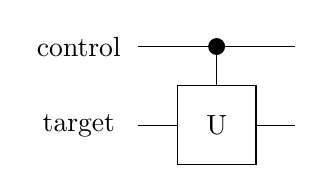
\begin{tikzpicture}[scale=.5] \node[draw=none] at (-3.5, 2) {control}; \node[draw=none] at (-3.5, 0) {target}; \draw (-2, 2) -- (2, 2); \draw[fill=black] (0, 2) circle (.2); \draw (0, 2) -- (0, 1); \draw (-2,0) -- (-1, 0); \draw (1, 0) -- (2, 0); \draw (-1,-1)--(-1,1)--(1,1)--(1,-1)--cycle; \node[draw=none] at (0, 0) {U}; \end{tikzpicture} } \]


\begin{DoxyParams}[1]{Parameters}
\mbox{\tt in,out}  & {\em multi\+Qubit} & object representing the set of all qubits \\
\hline
\mbox{\tt in}  & {\em control\+Qubit} & apply unitary if this qubit is 1 \\
\hline
\mbox{\tt in}  & {\em target\+Qubit} & qubit to operate on \\
\hline
\mbox{\tt in}  & {\em u} & single-\/qubit unitary matrix to apply \\
\hline
\end{DoxyParams}

\begin{DoxyExceptions}{Exceptions}
{\em exit\+With\+Error} & if either {\ttfamily control\+Qubit} or {\ttfamily target\+Qubit} are outside \mbox{[}0, {\ttfamily multi\+Qubit.\+num\+Qubits}) or are equal, or if {\ttfamily u} is not unitary. \\
\hline
\end{DoxyExceptions}


Definition at line 397 of file Qu\+E\+S\+T\+\_\+env\+\_\+mpi.\+c.



References Multi\+Qubit\+::chunk\+Id, chunk\+Is\+Upper(), controlled\+Unitary\+Distributed(), controlled\+Unitary\+Local(), exchange\+State\+Vectors(), get\+Chunk\+Pair\+Id(), get\+Rot\+Angle\+From\+Unitary\+Matrix(), half\+Matrix\+Block\+Fits\+In\+Chunk(), Multi\+Qubit\+::num\+Amps\+Per\+Chunk, Multi\+Qubit\+::num\+Qubits, Multi\+Qubit\+::pair\+State\+Vec, Qu\+E\+S\+T\+Assert(), Multi\+Qubit\+::state\+Vec, and validate\+Matrix\+Is\+Unitary().


\begin{DoxyCode}
399 \{
400     \mbox{\hyperlink{QuEST__env__mpi_8c_a3587b9d533e633ccf1abf9ad2ce45d8d}{QuESTAssert}}(targetQubit >= 0 && targetQubit < multiQubit.
      \mbox{\hyperlink{structMultiQubit_ab5b9795bdc6fb5855e1974dcbbaeb36f}{numQubits}}, 1, \_\_func\_\_);
401     \mbox{\hyperlink{QuEST__env__mpi_8c_a3587b9d533e633ccf1abf9ad2ce45d8d}{QuESTAssert}}(controlQubit >= 0 && controlQubit < multiQubit.
      \mbox{\hyperlink{structMultiQubit_ab5b9795bdc6fb5855e1974dcbbaeb36f}{numQubits}}, 2, \_\_func\_\_);
402     \mbox{\hyperlink{QuEST__env__mpi_8c_a3587b9d533e633ccf1abf9ad2ce45d8d}{QuESTAssert}}(controlQubit != targetQubit, 3, \_\_func\_\_);
403     \mbox{\hyperlink{QuEST__env__mpi_8c_a3587b9d533e633ccf1abf9ad2ce45d8d}{QuESTAssert}}(\mbox{\hyperlink{QuEST_8c_ae4fea133d1a8f09ff8da03038100adb2}{validateMatrixIsUnitary}}(u), 5, \_\_func\_\_);
404 
405     \textcolor{comment}{// flag to require memory exchange. 1: an entire block fits on one rank, 0: at most half a block fits
       on one rank}
406     \textcolor{keywordtype}{int} useLocalDataOnly = \mbox{\hyperlink{QuEST__env__mpi_8c_a4d043bb0cee54a5f94faf3ffc34a6790}{halfMatrixBlockFitsInChunk}}(multiQubit.
      \mbox{\hyperlink{structMultiQubit_a1cad83601a78635dd278259c7ed54f18}{numAmpsPerChunk}}, targetQubit);
407     \mbox{\hyperlink{structComplex}{Complex}} rot1, rot2;
408 
409     \textcolor{comment}{// rank's chunk is in upper half of block }
410     \textcolor{keywordtype}{int} rankIsUpper;
411     \textcolor{keywordtype}{int} pairRank; \textcolor{comment}{// rank of corresponding chunk}
412 
413     \textcolor{keywordflow}{if} (useLocalDataOnly)\{
414         \textcolor{comment}{// all values required to update state vector lie in this rank}
415         \mbox{\hyperlink{QuEST_8c_a8a4afcff70195a306c082b8ed8d4e09a}{controlledUnitaryLocal}}(multiQubit, controlQubit, targetQubit, u);
416     \} \textcolor{keywordflow}{else} \{
417         \textcolor{comment}{// need to get corresponding chunk of state vector from other rank}
418         rankIsUpper = \mbox{\hyperlink{QuEST__env__mpi_8c_a0552889d6f57d9e0ed8b209bf426482d}{chunkIsUpper}}(multiQubit.\mbox{\hyperlink{structMultiQubit_ab10c88249fa3825d6227ceec01d37e37}{chunkId}}, multiQubit.
      \mbox{\hyperlink{structMultiQubit_a1cad83601a78635dd278259c7ed54f18}{numAmpsPerChunk}}, targetQubit);
419         \mbox{\hyperlink{QuEST__env__mpi_8c_a5c9b2f129bdffaaba9857f6eddecbb17}{getRotAngleFromUnitaryMatrix}}(rankIsUpper, &rot1, &rot2, u);
420         pairRank = \mbox{\hyperlink{QuEST__env__mpi_8c_a7dba097f23f5d48dfdc9f3250444e2e4}{getChunkPairId}}(rankIsUpper, multiQubit.\mbox{\hyperlink{structMultiQubit_ab10c88249fa3825d6227ceec01d37e37}{chunkId}}, multiQubit.
      \mbox{\hyperlink{structMultiQubit_a1cad83601a78635dd278259c7ed54f18}{numAmpsPerChunk}}, targetQubit);
421         \textcolor{comment}{//printf("%d rank has pair rank: %d\(\backslash\)n", multiQubit.rank, pairRank);}
422         \textcolor{comment}{// get corresponding values from my pair}
423         \mbox{\hyperlink{QuEST__env__mpi_8c_a7682c9a3fd592d34ec15ba8fa172f104}{exchangeStateVectors}}(multiQubit, pairRank);
424 
425         \textcolor{comment}{// this rank's values are either in the upper of lower half of the block. send values to
       controlledUnitaryDistributed}
426         \textcolor{comment}{// in the correct order}
427         \textcolor{keywordflow}{if} (rankIsUpper)\{
428             \mbox{\hyperlink{QuEST_8c_a642093063a1f889f61a1311f6d6f2d3f}{controlledUnitaryDistributed}}(multiQubit,controlQubit,targetQubit,
      rot1,rot2,
429                     multiQubit.\mbox{\hyperlink{structMultiQubit_a45483190d6b01ef6b2f98f2bec9ab94f}{stateVec}}, \textcolor{comment}{//upper}
430                     multiQubit.\mbox{\hyperlink{structMultiQubit_a76f7db4eab52d2b30f58f973ada809c5}{pairStateVec}}, \textcolor{comment}{//lower}
431                     multiQubit.\mbox{\hyperlink{structMultiQubit_a45483190d6b01ef6b2f98f2bec9ab94f}{stateVec}}); \textcolor{comment}{//output}
432         \} \textcolor{keywordflow}{else} \{
433             \mbox{\hyperlink{QuEST_8c_a642093063a1f889f61a1311f6d6f2d3f}{controlledUnitaryDistributed}}(multiQubit,controlQubit,targetQubit,
      rot1,rot2,
434                     multiQubit.\mbox{\hyperlink{structMultiQubit_a76f7db4eab52d2b30f58f973ada809c5}{pairStateVec}}, \textcolor{comment}{//upper}
435                     multiQubit.\mbox{\hyperlink{structMultiQubit_a45483190d6b01ef6b2f98f2bec9ab94f}{stateVec}}, \textcolor{comment}{//lower}
436                     multiQubit.\mbox{\hyperlink{structMultiQubit_a45483190d6b01ef6b2f98f2bec9ab94f}{stateVec}}); \textcolor{comment}{//output}
437         \}
438     \}
439 \}
\end{DoxyCode}
\mbox{\Hypertarget{QuEST__env__mpi_8c_a7682c9a3fd592d34ec15ba8fa172f104}\label{QuEST__env__mpi_8c_a7682c9a3fd592d34ec15ba8fa172f104}} 
\index{Qu\+E\+S\+T\+\_\+env\+\_\+mpi.\+c@{Qu\+E\+S\+T\+\_\+env\+\_\+mpi.\+c}!exchange\+State\+Vectors@{exchange\+State\+Vectors}}
\index{exchange\+State\+Vectors@{exchange\+State\+Vectors}!Qu\+E\+S\+T\+\_\+env\+\_\+mpi.\+c@{Qu\+E\+S\+T\+\_\+env\+\_\+mpi.\+c}}
\paragraph{\texorpdfstring{exchange\+State\+Vectors()}{exchangeStateVectors()}}
{\footnotesize\ttfamily void exchange\+State\+Vectors (\begin{DoxyParamCaption}\item[{\mbox{\hyperlink{structMultiQubit}{Multi\+Qubit}}}]{multi\+Qubit,  }\item[{int}]{pair\+Rank }\end{DoxyParamCaption})}



Definition at line 242 of file Qu\+E\+S\+T\+\_\+env\+\_\+mpi.\+c.



References Complex\+Array\+::imag, M\+P\+I\+\_\+\+Qu\+E\+S\+T\+\_\+\+R\+E\+AL, Multi\+Qubit\+::num\+Amps\+Per\+Chunk, Multi\+Qubit\+::pair\+State\+Vec, Complex\+Array\+::real, R\+E\+AL, and Multi\+Qubit\+::state\+Vec.



Referenced by compact\+Unitary(), controlled\+Compact\+Unitary(), controlled\+Not(), controlled\+Unitary(), hadamard(), multi\+Controlled\+Unitary(), sigma\+X(), sigma\+Y(), and unitary().


\begin{DoxyCode}
242                                                               \{
243     \textcolor{comment}{// MPI send/receive vars}
244     \textcolor{keywordtype}{int} TAG=100;
245     MPI\_Status status;
246 
247     \textcolor{comment}{// Multiple messages are required as MPI uses int rather than long long int for count}
248     \textcolor{comment}{// For openmpi, messages are further restricted to 2GB in size -- do this for all cases}
249     \textcolor{comment}{// to be safe}
250     \textcolor{keywordtype}{long} \textcolor{keywordtype}{long} \textcolor{keywordtype}{int} maxMessageCount = 1LL<<29;
251     \textcolor{keywordflow}{if} (\textcolor{keyword}{sizeof}(\mbox{\hyperlink{QuEST__precision_8h_a4b654506f18b8bfd61ad2a29a7e38c25}{REAL}})==8) maxMessageCount = (1LL<<28);
252     \textcolor{keywordflow}{else} \textcolor{keywordflow}{if} (\textcolor{keyword}{sizeof}(\mbox{\hyperlink{QuEST__precision_8h_a4b654506f18b8bfd61ad2a29a7e38c25}{REAL}})==16) maxMessageCount = (1LL<<27);
253 
254     \textcolor{keywordflow}{if} (multiQubit.\mbox{\hyperlink{structMultiQubit_a1cad83601a78635dd278259c7ed54f18}{numAmpsPerChunk}}<maxMessageCount) maxMessageCount = multiQubit.
      \mbox{\hyperlink{structMultiQubit_a1cad83601a78635dd278259c7ed54f18}{numAmpsPerChunk}};
255     \textcolor{keywordtype}{int} numMessages = multiQubit.\mbox{\hyperlink{structMultiQubit_a1cad83601a78635dd278259c7ed54f18}{numAmpsPerChunk}}/maxMessageCount;
256     \textcolor{keywordtype}{int} i;
257     \textcolor{keywordtype}{long} \textcolor{keywordtype}{long} \textcolor{keywordtype}{int} offset;
258     \textcolor{comment}{// send my state vector to pairRank's multiQubit.pairStateVec}
259     \textcolor{comment}{// receive pairRank's state vector into multiQubit.pairStateVec}
260     \textcolor{keywordflow}{for} (i=0; i<numMessages; i++)\{
261         offset = i*maxMessageCount;
262         MPI\_Sendrecv(&multiQubit.\mbox{\hyperlink{structMultiQubit_a45483190d6b01ef6b2f98f2bec9ab94f}{stateVec}}.\mbox{\hyperlink{structComplexArray_a4195cac6c784ea1b6271f1c7dba1548a}{real}}[offset], maxMessageCount, 
      \mbox{\hyperlink{QuEST__precision_8h_a750ad290949ef7dc4afdfbd8231a5057}{MPI\_QuEST\_REAL}}, pairRank, TAG,
263                 &multiQubit.\mbox{\hyperlink{structMultiQubit_a76f7db4eab52d2b30f58f973ada809c5}{pairStateVec}}.\mbox{\hyperlink{structComplexArray_a4195cac6c784ea1b6271f1c7dba1548a}{real}}[offset], maxMessageCount, 
      \mbox{\hyperlink{QuEST__precision_8h_a750ad290949ef7dc4afdfbd8231a5057}{MPI\_QuEST\_REAL}},
264                 pairRank, TAG, MPI\_COMM\_WORLD, &status);
265         \textcolor{comment}{//printf("rank: %d err: %d\(\backslash\)n", multiQubit.rank, err);}
266         MPI\_Sendrecv(&multiQubit.\mbox{\hyperlink{structMultiQubit_a45483190d6b01ef6b2f98f2bec9ab94f}{stateVec}}.\mbox{\hyperlink{structComplexArray_a79dde47c7ae530c79cebfdf57b225968}{imag}}[offset], maxMessageCount, 
      \mbox{\hyperlink{QuEST__precision_8h_a750ad290949ef7dc4afdfbd8231a5057}{MPI\_QuEST\_REAL}}, pairRank, TAG,
267                 &multiQubit.\mbox{\hyperlink{structMultiQubit_a76f7db4eab52d2b30f58f973ada809c5}{pairStateVec}}.\mbox{\hyperlink{structComplexArray_a79dde47c7ae530c79cebfdf57b225968}{imag}}[offset], maxMessageCount, 
      \mbox{\hyperlink{QuEST__precision_8h_a750ad290949ef7dc4afdfbd8231a5057}{MPI\_QuEST\_REAL}},
268                 pairRank, TAG, MPI\_COMM\_WORLD, &status);
269     \}
270 \}
\end{DoxyCode}
\mbox{\Hypertarget{QuEST__env__mpi_8c_ae5f9019826f35e8b51b1716cfe397b45}\label{QuEST__env__mpi_8c_ae5f9019826f35e8b51b1716cfe397b45}} 
\index{Qu\+E\+S\+T\+\_\+env\+\_\+mpi.\+c@{Qu\+E\+S\+T\+\_\+env\+\_\+mpi.\+c}!exit\+With\+Error@{exit\+With\+Error}}
\index{exit\+With\+Error@{exit\+With\+Error}!Qu\+E\+S\+T\+\_\+env\+\_\+mpi.\+c@{Qu\+E\+S\+T\+\_\+env\+\_\+mpi.\+c}}
\paragraph{\texorpdfstring{exit\+With\+Error()}{exitWithError()}}
{\footnotesize\ttfamily void exit\+With\+Error (\begin{DoxyParamCaption}\item[{int}]{error\+Code,  }\item[{const char $\ast$}]{func }\end{DoxyParamCaption})}



Definition at line 752 of file Qu\+E\+S\+T\+\_\+env\+\_\+mpi.\+c.



References error\+Codes.



Referenced by Qu\+E\+S\+T\+Assert().


\begin{DoxyCode}
752                                                    \{
753     printf(\textcolor{stringliteral}{"!!!\(\backslash\)n"});
754     printf(\textcolor{stringliteral}{"QuEST Error in function %s: %s\(\backslash\)n"}, func, \mbox{\hyperlink{QuEST_8c_aac1637696885c75b73a1ecf381cea713}{errorCodes}}[errorCode]);
755     printf(\textcolor{stringliteral}{"!!!\(\backslash\)n"});
756     printf(\textcolor{stringliteral}{"exiting..\(\backslash\)n"});
757     MPI\_Abort(MPI\_COMM\_WORLD, errorCode);
758 \}
\end{DoxyCode}
\mbox{\Hypertarget{QuEST__env__mpi_8c_ad315c941a51bc053d39ebfa2040fd32e}\label{QuEST__env__mpi_8c_ad315c941a51bc053d39ebfa2040fd32e}} 
\index{Qu\+E\+S\+T\+\_\+env\+\_\+mpi.\+c@{Qu\+E\+S\+T\+\_\+env\+\_\+mpi.\+c}!find\+Probability\+Of\+Outcome@{find\+Probability\+Of\+Outcome}}
\index{find\+Probability\+Of\+Outcome@{find\+Probability\+Of\+Outcome}!Qu\+E\+S\+T\+\_\+env\+\_\+mpi.\+c@{Qu\+E\+S\+T\+\_\+env\+\_\+mpi.\+c}}
\paragraph{\texorpdfstring{find\+Probability\+Of\+Outcome()}{findProbabilityOfOutcome()}}
{\footnotesize\ttfamily \mbox{\hyperlink{QuEST__precision_8h_a4b654506f18b8bfd61ad2a29a7e38c25}{R\+E\+AL}} find\+Probability\+Of\+Outcome (\begin{DoxyParamCaption}\item[{\mbox{\hyperlink{structMultiQubit}{Multi\+Qubit}}}]{multi\+Qubit,  }\item[{const int}]{measure\+Qubit,  }\item[{int}]{outcome }\end{DoxyParamCaption})}



Gives the probability of a specified qubit being measured in the given outcome (0 or 1). 

This performs no actual measurement and does not change the state of the qubits.


\begin{DoxyParams}[1]{Parameters}
\mbox{\tt in}  & {\em multi\+Qubit} & object representing the set of all qubits \\
\hline
\mbox{\tt in}  & {\em measure\+Qubit} & qubit to study \\
\hline
\mbox{\tt in}  & {\em outcome} & for which to find the probability of the qubit being measured in \\
\hline
\end{DoxyParams}
\begin{DoxyReturn}{Returns}
probability of qubit measure\+Qubit being measured in the given outcome 
\end{DoxyReturn}

\begin{DoxyExceptions}{Exceptions}
{\em exit\+With\+Error} & if {\ttfamily measure\+Qubit} is outside \mbox{[}0, {\ttfamily multi\+Qubit.\+num\+Qubits}), or if {\ttfamily outcome} is not in \{0, 1\}. \\
\hline
\end{DoxyExceptions}


Definition at line 659 of file Qu\+E\+S\+T\+\_\+env\+\_\+mpi.\+c.



References Multi\+Qubit\+::chunk\+Id, find\+Probability\+Of\+Zero\+Distributed(), find\+Probability\+Of\+Zero\+Local(), half\+Matrix\+Block\+Fits\+In\+Chunk(), is\+Chunk\+To\+Skip\+In\+Find\+P\+Zero(), M\+P\+I\+\_\+\+Qu\+E\+S\+T\+\_\+\+R\+E\+AL, Multi\+Qubit\+::num\+Amps\+Per\+Chunk, Multi\+Qubit\+::num\+Qubits, Qu\+E\+S\+T\+Assert(), and R\+E\+AL.



Referenced by collapse\+To\+Outcome(), and measure\+With\+Stats().


\begin{DoxyCode}
660 \{
661     \mbox{\hyperlink{QuEST__env__mpi_8c_a3587b9d533e633ccf1abf9ad2ce45d8d}{QuESTAssert}}(measureQubit >= 0 && measureQubit < multiQubit.
      \mbox{\hyperlink{structMultiQubit_ab5b9795bdc6fb5855e1974dcbbaeb36f}{numQubits}}, 2, \_\_func\_\_);
662 
663     \mbox{\hyperlink{QuEST__precision_8h_a4b654506f18b8bfd61ad2a29a7e38c25}{REAL}} stateProb=0, totalStateProb=0;
664     \textcolor{keywordtype}{int} skipValuesWithinRank = \mbox{\hyperlink{QuEST__env__mpi_8c_a4d043bb0cee54a5f94faf3ffc34a6790}{halfMatrixBlockFitsInChunk}}(multiQubit.
      \mbox{\hyperlink{structMultiQubit_a1cad83601a78635dd278259c7ed54f18}{numAmpsPerChunk}}, measureQubit);
665     \textcolor{keywordflow}{if} (skipValuesWithinRank) \{
666         stateProb = \mbox{\hyperlink{QuEST_8c_a7c02cd0e1b4eac19771a0525f023249e}{findProbabilityOfZeroLocal}}(multiQubit, measureQubit);
667     \} \textcolor{keywordflow}{else} \{
668         \textcolor{keywordflow}{if} (!\mbox{\hyperlink{QuEST__env__mpi_8c_af0ea25f00987af4c53f17c9cca62ab41}{isChunkToSkipInFindPZero}}(multiQubit.\mbox{\hyperlink{structMultiQubit_ab10c88249fa3825d6227ceec01d37e37}{chunkId}}, multiQubit.
      \mbox{\hyperlink{structMultiQubit_a1cad83601a78635dd278259c7ed54f18}{numAmpsPerChunk}}, measureQubit))\{
669             stateProb = \mbox{\hyperlink{QuEST_8c_a9ac9bb717a889f09d307eda9f0b65957}{findProbabilityOfZeroDistributed}}(multiQubit, 
      measureQubit);
670         \} \textcolor{keywordflow}{else} stateProb = 0;
671     \}
672     MPI\_Allreduce(&stateProb, &totalStateProb, 1, \mbox{\hyperlink{QuEST__precision_8h_a750ad290949ef7dc4afdfbd8231a5057}{MPI\_QuEST\_REAL}}, MPI\_SUM, MPI\_COMM\_WORLD);
673     \textcolor{keywordflow}{if} (outcome==1) totalStateProb = 1.0 - totalStateProb;
674     \textcolor{keywordflow}{return} totalStateProb;
675 \}
\end{DoxyCode}
\mbox{\Hypertarget{QuEST__env__mpi_8c_a8605e6a6295174cb4661156eaa709ec4}\label{QuEST__env__mpi_8c_a8605e6a6295174cb4661156eaa709ec4}} 
\index{Qu\+E\+S\+T\+\_\+env\+\_\+mpi.\+c@{Qu\+E\+S\+T\+\_\+env\+\_\+mpi.\+c}!get\+Chunk\+Id\+From\+Index@{get\+Chunk\+Id\+From\+Index}}
\index{get\+Chunk\+Id\+From\+Index@{get\+Chunk\+Id\+From\+Index}!Qu\+E\+S\+T\+\_\+env\+\_\+mpi.\+c@{Qu\+E\+S\+T\+\_\+env\+\_\+mpi.\+c}}
\paragraph{\texorpdfstring{get\+Chunk\+Id\+From\+Index()}{getChunkIdFromIndex()}}
{\footnotesize\ttfamily int get\+Chunk\+Id\+From\+Index (\begin{DoxyParamCaption}\item[{\mbox{\hyperlink{structMultiQubit}{Multi\+Qubit}}}]{multi\+Qubit,  }\item[{long long int}]{index }\end{DoxyParamCaption})\hspace{0.3cm}{\ttfamily [static]}}



Definition at line 88 of file Qu\+E\+S\+T\+\_\+env\+\_\+mpi.\+c.



References Multi\+Qubit\+::num\+Amps\+Per\+Chunk.



Referenced by get\+Imag\+Amp\+El(), and get\+Real\+Amp\+El().


\begin{DoxyCode}
88                                                                    \{
89     \textcolor{keywordflow}{return} index/multiQubit.\mbox{\hyperlink{structMultiQubit_a1cad83601a78635dd278259c7ed54f18}{numAmpsPerChunk}}; \textcolor{comment}{// this is numAmpsPerChunk}
90 \}
\end{DoxyCode}
\mbox{\Hypertarget{QuEST__env__mpi_8c_a7dba097f23f5d48dfdc9f3250444e2e4}\label{QuEST__env__mpi_8c_a7dba097f23f5d48dfdc9f3250444e2e4}} 
\index{Qu\+E\+S\+T\+\_\+env\+\_\+mpi.\+c@{Qu\+E\+S\+T\+\_\+env\+\_\+mpi.\+c}!get\+Chunk\+Pair\+Id@{get\+Chunk\+Pair\+Id}}
\index{get\+Chunk\+Pair\+Id@{get\+Chunk\+Pair\+Id}!Qu\+E\+S\+T\+\_\+env\+\_\+mpi.\+c@{Qu\+E\+S\+T\+\_\+env\+\_\+mpi.\+c}}
\paragraph{\texorpdfstring{get\+Chunk\+Pair\+Id()}{getChunkPairId()}}
{\footnotesize\ttfamily static int get\+Chunk\+Pair\+Id (\begin{DoxyParamCaption}\item[{int}]{chunk\+Is\+Upper,  }\item[{int}]{chunk\+Id,  }\item[{long long int}]{chunk\+Size,  }\item[{int}]{target\+Qubit }\end{DoxyParamCaption})\hspace{0.3cm}{\ttfamily [static]}}



get position of corresponding chunk, holding values required to update values in my chunk (with chunk\+Id) when rotating target\+Qubit. 


\begin{DoxyParams}[1]{Parameters}
\mbox{\tt in}  & {\em chunk\+Is\+Upper} & 1\+: chunk is in upper half of block, 0\+: chunk is in lower half \\
\hline
\mbox{\tt in}  & {\em chunk\+Id} & id of chunk in state vector \\
\hline
\mbox{\tt in}  & {\em chunk\+Size} & number of amps in chunk \\
\hline
\mbox{\tt in}  & {\em target\+Qubit} & qubit being rotated \\
\hline
\end{DoxyParams}
\begin{DoxyReturn}{Returns}
chunk\+Id of chunk required to rotate target\+Qubit 
\end{DoxyReturn}


Definition at line 217 of file Qu\+E\+S\+T\+\_\+env\+\_\+mpi.\+c.



References chunk\+Is\+Upper().



Referenced by compact\+Unitary(), controlled\+Compact\+Unitary(), controlled\+Not(), controlled\+Unitary(), hadamard(), multi\+Controlled\+Unitary(), sigma\+X(), sigma\+Y(), and unitary().


\begin{DoxyCode}
218 \{
219     \textcolor{keywordtype}{long} \textcolor{keywordtype}{long} \textcolor{keywordtype}{int} sizeHalfBlock = 1LL << (targetQubit);
220     \textcolor{keywordtype}{int} chunksPerHalfBlock = sizeHalfBlock/chunkSize;
221     \textcolor{keywordflow}{if} (\mbox{\hyperlink{QuEST__env__mpi_8c_a0552889d6f57d9e0ed8b209bf426482d}{chunkIsUpper}})\{
222         \textcolor{keywordflow}{return} chunkId + chunksPerHalfBlock;
223     \} \textcolor{keywordflow}{else} \{
224         \textcolor{keywordflow}{return} chunkId - chunksPerHalfBlock;
225     \}
226 \}
\end{DoxyCode}
\mbox{\Hypertarget{QuEST__env__mpi_8c_a3615f76fd5f57008d9b74bbd10533dd0}\label{QuEST__env__mpi_8c_a3615f76fd5f57008d9b74bbd10533dd0}} 
\index{Qu\+E\+S\+T\+\_\+env\+\_\+mpi.\+c@{Qu\+E\+S\+T\+\_\+env\+\_\+mpi.\+c}!get\+Imag\+Amp\+El@{get\+Imag\+Amp\+El}}
\index{get\+Imag\+Amp\+El@{get\+Imag\+Amp\+El}!Qu\+E\+S\+T\+\_\+env\+\_\+mpi.\+c@{Qu\+E\+S\+T\+\_\+env\+\_\+mpi.\+c}}
\paragraph{\texorpdfstring{get\+Imag\+Amp\+El()}{getImagAmpEl()}}
{\footnotesize\ttfamily \mbox{\hyperlink{QuEST__precision_8h_a4b654506f18b8bfd61ad2a29a7e38c25}{R\+E\+AL}} get\+Imag\+Amp\+El (\begin{DoxyParamCaption}\item[{\mbox{\hyperlink{structMultiQubit}{Multi\+Qubit}}}]{multi\+Qubit,  }\item[{long long int}]{index }\end{DoxyParamCaption})}



Get the imaginary component of the complex probability amplitude at an index in the state vector. 

For debugging purposes.


\begin{DoxyParams}[1]{Parameters}
\mbox{\tt in}  & {\em multi\+Qubit} & object representing a set of qubits \\
\hline
\mbox{\tt in}  & {\em index} & index in state vector of probability amplitudes \\
\hline
\end{DoxyParams}
\begin{DoxyReturn}{Returns}
imaginary component at that index 
\end{DoxyReturn}

\begin{DoxyExceptions}{Exceptions}
{\em exit\+With\+Error} & if {\ttfamily index} is outside \mbox{[}0, $2^{N}$) where $N = $ {\ttfamily multi\+Qubit.\+num\+Qubits} \\
\hline
\end{DoxyExceptions}


Definition at line 102 of file Qu\+E\+S\+T\+\_\+env\+\_\+mpi.\+c.



References Multi\+Qubit\+::chunk\+Id, get\+Chunk\+Id\+From\+Index(), Complex\+Array\+::imag, M\+P\+I\+\_\+\+Qu\+E\+S\+T\+\_\+\+R\+E\+AL, Multi\+Qubit\+::num\+Amps\+Per\+Chunk, R\+E\+AL, and Multi\+Qubit\+::state\+Vec.


\begin{DoxyCode}
102                                                              \{
103     \textcolor{keywordtype}{int} chunkId = \mbox{\hyperlink{QuEST__env__mpi_8c_a8605e6a6295174cb4661156eaa709ec4}{getChunkIdFromIndex}}(multiQubit, index);
104     \mbox{\hyperlink{QuEST__precision_8h_a4b654506f18b8bfd61ad2a29a7e38c25}{REAL}} el; 
105     \textcolor{keywordflow}{if} (multiQubit.\mbox{\hyperlink{structMultiQubit_ab10c88249fa3825d6227ceec01d37e37}{chunkId}}==chunkId)\{
106         el = multiQubit.\mbox{\hyperlink{structMultiQubit_a45483190d6b01ef6b2f98f2bec9ab94f}{stateVec}}.\mbox{\hyperlink{structComplexArray_a79dde47c7ae530c79cebfdf57b225968}{imag}}[index-chunkId*multiQubit.
      \mbox{\hyperlink{structMultiQubit_a1cad83601a78635dd278259c7ed54f18}{numAmpsPerChunk}}];
107     \}
108     MPI\_Bcast(&el, 1, \mbox{\hyperlink{QuEST__precision_8h_a750ad290949ef7dc4afdfbd8231a5057}{MPI\_QuEST\_REAL}}, chunkId, MPI\_COMM\_WORLD);
109     \textcolor{keywordflow}{return} el; 
110 \}
\end{DoxyCode}
\mbox{\Hypertarget{QuEST__env__mpi_8c_a317b786f577fa6bc136ea7f0ee7330a7}\label{QuEST__env__mpi_8c_a317b786f577fa6bc136ea7f0ee7330a7}} 
\index{Qu\+E\+S\+T\+\_\+env\+\_\+mpi.\+c@{Qu\+E\+S\+T\+\_\+env\+\_\+mpi.\+c}!get\+Real\+Amp\+El@{get\+Real\+Amp\+El}}
\index{get\+Real\+Amp\+El@{get\+Real\+Amp\+El}!Qu\+E\+S\+T\+\_\+env\+\_\+mpi.\+c@{Qu\+E\+S\+T\+\_\+env\+\_\+mpi.\+c}}
\paragraph{\texorpdfstring{get\+Real\+Amp\+El()}{getRealAmpEl()}}
{\footnotesize\ttfamily \mbox{\hyperlink{QuEST__precision_8h_a4b654506f18b8bfd61ad2a29a7e38c25}{R\+E\+AL}} get\+Real\+Amp\+El (\begin{DoxyParamCaption}\item[{\mbox{\hyperlink{structMultiQubit}{Multi\+Qubit}}}]{multi\+Qubit,  }\item[{long long int}]{index }\end{DoxyParamCaption})}



Get the real component of the complex probability amplitude at an index in the state vector. 

For debugging purposes.


\begin{DoxyParams}[1]{Parameters}
\mbox{\tt in}  & {\em multi\+Qubit} & object representing a set of qubits \\
\hline
\mbox{\tt in}  & {\em index} & index in state vector of probability amplitudes \\
\hline
\end{DoxyParams}
\begin{DoxyReturn}{Returns}
real component at that index 
\end{DoxyReturn}

\begin{DoxyExceptions}{Exceptions}
{\em exit\+With\+Error} & if {\ttfamily index} is outside \mbox{[}0, $2^{N}$) where $N = $ {\ttfamily multi\+Qubit.\+num\+Qubits} \\
\hline
\end{DoxyExceptions}


Definition at line 92 of file Qu\+E\+S\+T\+\_\+env\+\_\+mpi.\+c.



References Multi\+Qubit\+::chunk\+Id, get\+Chunk\+Id\+From\+Index(), M\+P\+I\+\_\+\+Qu\+E\+S\+T\+\_\+\+R\+E\+AL, Multi\+Qubit\+::num\+Amps\+Per\+Chunk, Complex\+Array\+::real, R\+E\+AL, and Multi\+Qubit\+::state\+Vec.


\begin{DoxyCode}
92                                                              \{
93     \textcolor{keywordtype}{int} chunkId = \mbox{\hyperlink{QuEST__env__mpi_8c_a8605e6a6295174cb4661156eaa709ec4}{getChunkIdFromIndex}}(multiQubit, index);
94     \mbox{\hyperlink{QuEST__precision_8h_a4b654506f18b8bfd61ad2a29a7e38c25}{REAL}} el; 
95     \textcolor{keywordflow}{if} (multiQubit.\mbox{\hyperlink{structMultiQubit_ab10c88249fa3825d6227ceec01d37e37}{chunkId}}==chunkId)\{
96         el = multiQubit.\mbox{\hyperlink{structMultiQubit_a45483190d6b01ef6b2f98f2bec9ab94f}{stateVec}}.\mbox{\hyperlink{structComplexArray_a4195cac6c784ea1b6271f1c7dba1548a}{real}}[index-chunkId*multiQubit.
      \mbox{\hyperlink{structMultiQubit_a1cad83601a78635dd278259c7ed54f18}{numAmpsPerChunk}}];
97     \}
98     MPI\_Bcast(&el, 1, \mbox{\hyperlink{QuEST__precision_8h_a750ad290949ef7dc4afdfbd8231a5057}{MPI\_QuEST\_REAL}}, chunkId, MPI\_COMM\_WORLD);
99     \textcolor{keywordflow}{return} el; 
100 \} 
\end{DoxyCode}
\mbox{\Hypertarget{QuEST__env__mpi_8c_adb4b0373425b282abed27742d0ce0872}\label{QuEST__env__mpi_8c_adb4b0373425b282abed27742d0ce0872}} 
\index{Qu\+E\+S\+T\+\_\+env\+\_\+mpi.\+c@{Qu\+E\+S\+T\+\_\+env\+\_\+mpi.\+c}!get\+Rot\+Angle@{get\+Rot\+Angle}}
\index{get\+Rot\+Angle@{get\+Rot\+Angle}!Qu\+E\+S\+T\+\_\+env\+\_\+mpi.\+c@{Qu\+E\+S\+T\+\_\+env\+\_\+mpi.\+c}}
\paragraph{\texorpdfstring{get\+Rot\+Angle()}{getRotAngle()}}
{\footnotesize\ttfamily static void get\+Rot\+Angle (\begin{DoxyParamCaption}\item[{int}]{chunk\+Is\+Upper,  }\item[{\mbox{\hyperlink{structComplex}{Complex}} $\ast$}]{rot1,  }\item[{\mbox{\hyperlink{structComplex}{Complex}} $\ast$}]{rot2,  }\item[{\mbox{\hyperlink{structComplex}{Complex}}}]{alpha,  }\item[{\mbox{\hyperlink{structComplex}{Complex}}}]{beta }\end{DoxyParamCaption})\hspace{0.3cm}{\ttfamily [static]}}



Get rotation values for a given chunk. 


\begin{DoxyParams}[1]{Parameters}
\mbox{\tt in}  & {\em chunk\+Is\+Upper} & 1\+: chunk is in upper half of block, 0\+: chunk is in lower half\\
\hline
\mbox{\tt out}  & {\em rot1,rot2} & rotation values to use, allocated for upper/lower such that \begin{DoxyVerb}stateUpper = rot1 * stateUpper + conj(rot2)  * stateLower
\end{DoxyVerb}
 or \begin{DoxyVerb}stateLower = rot1 * stateUpper + conj(rot2)  * stateLower
\end{DoxyVerb}
\\
\hline
\mbox{\tt in}  & {\em alpha,beta} & initial rotation values \\
\hline
\end{DoxyParams}


Definition at line 172 of file Qu\+E\+S\+T\+\_\+env\+\_\+mpi.\+c.



References chunk\+Is\+Upper(), Complex\+::imag, and Complex\+::real.



Referenced by compact\+Unitary(), and controlled\+Compact\+Unitary().


\begin{DoxyCode}
173 \{
174     \textcolor{keywordflow}{if} (\mbox{\hyperlink{QuEST__env__mpi_8c_a0552889d6f57d9e0ed8b209bf426482d}{chunkIsUpper}})\{
175         *rot1=alpha;
176         rot2->\mbox{\hyperlink{structComplex_a479ad939835457595fcca3ca55c06283}{real}}=-beta.\mbox{\hyperlink{structComplex_a479ad939835457595fcca3ca55c06283}{real}};
177         rot2->\mbox{\hyperlink{structComplex_a1151948284b21c0052f203f23ab931d9}{imag}}=-beta.\mbox{\hyperlink{structComplex_a1151948284b21c0052f203f23ab931d9}{imag}};
178     \} \textcolor{keywordflow}{else} \{
179         *rot1=beta;
180         *rot2=alpha;
181     \}
182 \}
\end{DoxyCode}
\mbox{\Hypertarget{QuEST__env__mpi_8c_a5c9b2f129bdffaaba9857f6eddecbb17}\label{QuEST__env__mpi_8c_a5c9b2f129bdffaaba9857f6eddecbb17}} 
\index{Qu\+E\+S\+T\+\_\+env\+\_\+mpi.\+c@{Qu\+E\+S\+T\+\_\+env\+\_\+mpi.\+c}!get\+Rot\+Angle\+From\+Unitary\+Matrix@{get\+Rot\+Angle\+From\+Unitary\+Matrix}}
\index{get\+Rot\+Angle\+From\+Unitary\+Matrix@{get\+Rot\+Angle\+From\+Unitary\+Matrix}!Qu\+E\+S\+T\+\_\+env\+\_\+mpi.\+c@{Qu\+E\+S\+T\+\_\+env\+\_\+mpi.\+c}}
\paragraph{\texorpdfstring{get\+Rot\+Angle\+From\+Unitary\+Matrix()}{getRotAngleFromUnitaryMatrix()}}
{\footnotesize\ttfamily static void get\+Rot\+Angle\+From\+Unitary\+Matrix (\begin{DoxyParamCaption}\item[{int}]{chunk\+Is\+Upper,  }\item[{\mbox{\hyperlink{structComplex}{Complex}} $\ast$}]{rot1,  }\item[{\mbox{\hyperlink{structComplex}{Complex}} $\ast$}]{rot2,  }\item[{\mbox{\hyperlink{structComplexMatrix2}{Complex\+Matrix2}}}]{u }\end{DoxyParamCaption})\hspace{0.3cm}{\ttfamily [static]}}



Get rotation values for a given chunk given a unitary matrix. 


\begin{DoxyParams}[1]{Parameters}
\mbox{\tt in}  & {\em chunk\+Is\+Upper} & 1\+: chunk is in upper half of block, 0\+: chunk is in lower half\\
\hline
\mbox{\tt out}  & {\em rot1,rot2} & rotation values to use, allocated for upper/lower such that \begin{DoxyVerb}stateUpper = rot1 * stateUpper + conj(rot2)  * stateLower
\end{DoxyVerb}
 or \begin{DoxyVerb}stateLower = rot1 * stateUpper + conj(rot2)  * stateLower
\end{DoxyVerb}
 \\
\hline
\mbox{\tt in}  & {\em u} & unitary matrix operation \\
\hline
\end{DoxyParams}


Definition at line 197 of file Qu\+E\+S\+T\+\_\+env\+\_\+mpi.\+c.



References chunk\+Is\+Upper(), Complex\+Matrix2\+::r0c0, Complex\+Matrix2\+::r0c1, Complex\+Matrix2\+::r1c0, and Complex\+Matrix2\+::r1c1.



Referenced by controlled\+Unitary(), multi\+Controlled\+Unitary(), and unitary().


\begin{DoxyCode}
198 \{
199     \textcolor{keywordflow}{if} (\mbox{\hyperlink{QuEST__env__mpi_8c_a0552889d6f57d9e0ed8b209bf426482d}{chunkIsUpper}})\{
200         *rot1=u.\mbox{\hyperlink{structComplexMatrix2_ae72b4458233b077a636beee1892e81ff}{r0c0}};
201         *rot2=u.\mbox{\hyperlink{structComplexMatrix2_a0f3932f055a8b05cef361bce25d51172}{r0c1}};
202     \} \textcolor{keywordflow}{else} \{
203         *rot1=u.\mbox{\hyperlink{structComplexMatrix2_ab98282015ed2065e53fbc9638e2583ab}{r1c0}};
204         *rot2=u.\mbox{\hyperlink{structComplexMatrix2_a763007c3070802373549ba0350f83c8a}{r1c1}};
205     \}
206 \}
\end{DoxyCode}
\mbox{\Hypertarget{QuEST__env__mpi_8c_aa09b5dd93de6df1384b8f2c0041749ab}\label{QuEST__env__mpi_8c_aa09b5dd93de6df1384b8f2c0041749ab}} 
\index{Qu\+E\+S\+T\+\_\+env\+\_\+mpi.\+c@{Qu\+E\+S\+T\+\_\+env\+\_\+mpi.\+c}!hadamard@{hadamard}}
\index{hadamard@{hadamard}!Qu\+E\+S\+T\+\_\+env\+\_\+mpi.\+c@{Qu\+E\+S\+T\+\_\+env\+\_\+mpi.\+c}}
\paragraph{\texorpdfstring{hadamard()}{hadamard()}}
{\footnotesize\ttfamily void hadamard (\begin{DoxyParamCaption}\item[{\mbox{\hyperlink{structMultiQubit}{Multi\+Qubit}}}]{multi\+Qubit,  }\item[{const int}]{target\+Qubit }\end{DoxyParamCaption})}



Apply the single-\/qubit Hadamard gate. 

This takes $|0\rangle$ to $|+\rangle$ and $|1\rangle$ to $|-\rangle$, and is equivalent to a rotation of $\pi$ around the x-\/axis then $\pi/2$ about the y-\/axis on the Bloch-\/sphere. I.\+e. \[ \frac{1}{\sqrt{2}} \begin{pmatrix} 1 & 1 \\ 1 & -1 \end{pmatrix} \] ~\newline
 \[ \setlength{\fboxrule}{0.01pt} \fbox{ 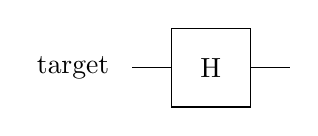
\begin{tikzpicture}[scale=.5] \node[draw=none] at (-3.5, 0) {target}; \draw (-2,0) -- (-1, 0); \draw (1, 0) -- (2, 0); \draw (-1,-1)--(-1,1)--(1,1)--(1,-1)--cycle; \node[draw=none] at (0, 0) {H}; \end{tikzpicture} } \] ~\newline
 
\begin{DoxyParams}[1]{Parameters}
\mbox{\tt in,out}  & {\em multi\+Qubit} & object representing the set of all qubits \\
\hline
\mbox{\tt in}  & {\em target\+Qubit} & qubit to operate on \\
\hline
\end{DoxyParams}

\begin{DoxyExceptions}{Exceptions}
{\em exit\+With\+Error} & if {\ttfamily target\+Qubit} is outside \mbox{[}0, {\ttfamily multi\+Qubit.\+num\+Qubits}). \\
\hline
\end{DoxyExceptions}


Definition at line 602 of file Qu\+E\+S\+T\+\_\+env\+\_\+mpi.\+c.



References Multi\+Qubit\+::chunk\+Id, chunk\+Is\+Upper(), exchange\+State\+Vectors(), get\+Chunk\+Pair\+Id(), hadamard\+Distributed(), hadamard\+Local(), half\+Matrix\+Block\+Fits\+In\+Chunk(), Multi\+Qubit\+::num\+Amps\+Per\+Chunk, Multi\+Qubit\+::num\+Qubits, Multi\+Qubit\+::pair\+State\+Vec, Qu\+E\+S\+T\+Assert(), and Multi\+Qubit\+::state\+Vec.


\begin{DoxyCode}
603 \{
604     \mbox{\hyperlink{QuEST__env__mpi_8c_a3587b9d533e633ccf1abf9ad2ce45d8d}{QuESTAssert}}(targetQubit >= 0 && targetQubit < multiQubit.
      \mbox{\hyperlink{structMultiQubit_ab5b9795bdc6fb5855e1974dcbbaeb36f}{numQubits}}, 1, \_\_func\_\_);
605 
606     \textcolor{comment}{// flag to require memory exchange. 1: an entire block fits on one rank, 0: at most half a block fits
       on one rank}
607     \textcolor{keywordtype}{int} useLocalDataOnly = \mbox{\hyperlink{QuEST__env__mpi_8c_a4d043bb0cee54a5f94faf3ffc34a6790}{halfMatrixBlockFitsInChunk}}(multiQubit.
      \mbox{\hyperlink{structMultiQubit_a1cad83601a78635dd278259c7ed54f18}{numAmpsPerChunk}}, targetQubit);
608 
609     \textcolor{comment}{// rank's chunk is in upper half of block }
610     \textcolor{keywordtype}{int} rankIsUpper;
611     \textcolor{keywordtype}{int} pairRank; \textcolor{comment}{// rank of corresponding chunk}
612 
613     \textcolor{keywordflow}{if} (useLocalDataOnly)\{
614         \textcolor{comment}{// all values required to update state vector lie in this rank}
615         \mbox{\hyperlink{QuEST_8c_aa9f0718b4dd794a3e1b143e3b153bfc5}{hadamardLocal}}(multiQubit, targetQubit);
616     \} \textcolor{keywordflow}{else} \{
617         \textcolor{comment}{// need to get corresponding chunk of state vector from other rank}
618         rankIsUpper = \mbox{\hyperlink{QuEST__env__mpi_8c_a0552889d6f57d9e0ed8b209bf426482d}{chunkIsUpper}}(multiQubit.\mbox{\hyperlink{structMultiQubit_ab10c88249fa3825d6227ceec01d37e37}{chunkId}}, multiQubit.
      \mbox{\hyperlink{structMultiQubit_a1cad83601a78635dd278259c7ed54f18}{numAmpsPerChunk}}, targetQubit);
619         pairRank = \mbox{\hyperlink{QuEST__env__mpi_8c_a7dba097f23f5d48dfdc9f3250444e2e4}{getChunkPairId}}(rankIsUpper, multiQubit.\mbox{\hyperlink{structMultiQubit_ab10c88249fa3825d6227ceec01d37e37}{chunkId}}, multiQubit.
      \mbox{\hyperlink{structMultiQubit_a1cad83601a78635dd278259c7ed54f18}{numAmpsPerChunk}}, targetQubit);
620         \textcolor{comment}{//printf("%d rank has pair rank: %d\(\backslash\)n", multiQubit.rank, pairRank);}
621         \textcolor{comment}{// get corresponding values from my pair}
622         \mbox{\hyperlink{QuEST__env__mpi_8c_a7682c9a3fd592d34ec15ba8fa172f104}{exchangeStateVectors}}(multiQubit, pairRank);
623         \textcolor{comment}{// this rank's values are either in the upper of lower half of the block. send values to
       hadamardDistributed}
624         \textcolor{comment}{// in the correct order}
625         \textcolor{keywordflow}{if} (rankIsUpper)\{
626             \mbox{\hyperlink{QuEST_8c_ae6a897066979fc52d977007d959ca09d}{hadamardDistributed}}(multiQubit,targetQubit,
627                     multiQubit.\mbox{\hyperlink{structMultiQubit_a45483190d6b01ef6b2f98f2bec9ab94f}{stateVec}}, \textcolor{comment}{//upper}
628                     multiQubit.\mbox{\hyperlink{structMultiQubit_a76f7db4eab52d2b30f58f973ada809c5}{pairStateVec}}, \textcolor{comment}{//lower}
629                     multiQubit.\mbox{\hyperlink{structMultiQubit_a45483190d6b01ef6b2f98f2bec9ab94f}{stateVec}}, rankIsUpper); \textcolor{comment}{//output}
630         \} \textcolor{keywordflow}{else} \{
631             \mbox{\hyperlink{QuEST_8c_ae6a897066979fc52d977007d959ca09d}{hadamardDistributed}}(multiQubit,targetQubit,
632                     multiQubit.\mbox{\hyperlink{structMultiQubit_a76f7db4eab52d2b30f58f973ada809c5}{pairStateVec}}, \textcolor{comment}{//upper}
633                     multiQubit.\mbox{\hyperlink{structMultiQubit_a45483190d6b01ef6b2f98f2bec9ab94f}{stateVec}}, \textcolor{comment}{//lower}
634                     multiQubit.\mbox{\hyperlink{structMultiQubit_a45483190d6b01ef6b2f98f2bec9ab94f}{stateVec}}, rankIsUpper); \textcolor{comment}{//output}
635         \}
636     \}
637 \}
\end{DoxyCode}
\mbox{\Hypertarget{QuEST__env__mpi_8c_a4d043bb0cee54a5f94faf3ffc34a6790}\label{QuEST__env__mpi_8c_a4d043bb0cee54a5f94faf3ffc34a6790}} 
\index{Qu\+E\+S\+T\+\_\+env\+\_\+mpi.\+c@{Qu\+E\+S\+T\+\_\+env\+\_\+mpi.\+c}!half\+Matrix\+Block\+Fits\+In\+Chunk@{half\+Matrix\+Block\+Fits\+In\+Chunk}}
\index{half\+Matrix\+Block\+Fits\+In\+Chunk@{half\+Matrix\+Block\+Fits\+In\+Chunk}!Qu\+E\+S\+T\+\_\+env\+\_\+mpi.\+c@{Qu\+E\+S\+T\+\_\+env\+\_\+mpi.\+c}}
\paragraph{\texorpdfstring{half\+Matrix\+Block\+Fits\+In\+Chunk()}{halfMatrixBlockFitsInChunk()}}
{\footnotesize\ttfamily static int half\+Matrix\+Block\+Fits\+In\+Chunk (\begin{DoxyParamCaption}\item[{long long int}]{chunk\+Size,  }\item[{int}]{target\+Qubit }\end{DoxyParamCaption})\hspace{0.3cm}{\ttfamily [static]}}



return whether the current qubit rotation will use blocks that fit within a single chunk. 


\begin{DoxyParams}[1]{Parameters}
\mbox{\tt in}  & {\em chunk\+Size} & number of amps in chunk \\
\hline
\mbox{\tt in}  & {\em target\+Qubit} & qubit being rotated \\
\hline
\end{DoxyParams}
\begin{DoxyReturn}{Returns}
1\+: one chunk fits in one block 0\+: chunk is larger than block 
\end{DoxyReturn}


Definition at line 235 of file Qu\+E\+S\+T\+\_\+env\+\_\+mpi.\+c.



Referenced by collapse\+To\+Outcome(), compact\+Unitary(), controlled\+Compact\+Unitary(), controlled\+Not(), controlled\+Unitary(), find\+Probability\+Of\+Outcome(), hadamard(), measure\+With\+Stats(), multi\+Controlled\+Unitary(), phase\+Gate(), sigma\+X(), sigma\+Y(), and unitary().


\begin{DoxyCode}
236 \{
237     \textcolor{keywordtype}{long} \textcolor{keywordtype}{long} \textcolor{keywordtype}{int} sizeHalfBlock = 1LL << (targetQubit);
238     \textcolor{keywordflow}{if} (chunkSize > sizeHalfBlock) \textcolor{keywordflow}{return} 1;
239     \textcolor{keywordflow}{else} \textcolor{keywordflow}{return} 0;
240 \}
\end{DoxyCode}
\mbox{\Hypertarget{QuEST__env__mpi_8c_ad84a3ce68d1ca02b4e3f741ea45b6054}\label{QuEST__env__mpi_8c_ad84a3ce68d1ca02b4e3f741ea45b6054}} 
\index{Qu\+E\+S\+T\+\_\+env\+\_\+mpi.\+c@{Qu\+E\+S\+T\+\_\+env\+\_\+mpi.\+c}!init\+Qu\+E\+S\+T\+Env@{init\+Qu\+E\+S\+T\+Env}}
\index{init\+Qu\+E\+S\+T\+Env@{init\+Qu\+E\+S\+T\+Env}!Qu\+E\+S\+T\+\_\+env\+\_\+mpi.\+c@{Qu\+E\+S\+T\+\_\+env\+\_\+mpi.\+c}}
\paragraph{\texorpdfstring{init\+Qu\+E\+S\+T\+Env()}{initQuESTEnv()}}
{\footnotesize\ttfamily void init\+Qu\+E\+S\+T\+Env (\begin{DoxyParamCaption}\item[{\mbox{\hyperlink{structQuESTEnv}{Qu\+E\+S\+T\+Env}} $\ast$}]{env }\end{DoxyParamCaption})}



Initialize the Qu\+E\+ST environment. 

If something needs to be done to set up the execution environment, such as initializing M\+PI when running in distributed mode, it is handled here


\begin{DoxyParams}[1]{Parameters}
\mbox{\tt in,out}  & {\em env} & object representing the execution environment. A single instance is used for each program \\
\hline
\end{DoxyParams}


Definition at line 33 of file Qu\+E\+S\+T\+\_\+env\+\_\+mpi.\+c.



References env, Qu\+E\+S\+T\+Env\+::num\+Ranks, Qu\+E\+S\+T\+Env\+::rank, and seed\+Qu\+E\+S\+T\+Default().


\begin{DoxyCode}
33                                 \{
34     \textcolor{comment}{// init MPI environment}
35     \textcolor{keywordtype}{int} rank, numRanks, initialized;
36     MPI\_Initialized(&initialized);
37     \textcolor{keywordflow}{if} (!initialized)\{
38         MPI\_Init(NULL, NULL);
39         MPI\_Comm\_size(MPI\_COMM\_WORLD, &numRanks);
40         MPI\_Comm\_rank(MPI\_COMM\_WORLD, &rank);
41 
42         \mbox{\hyperlink{runTests_8c_a5fd8ba97fcae3408ae6221dfc3cc1f93}{env}}->\mbox{\hyperlink{structQuESTEnv_aa648bb336cf8598467cb62db00b9cee8}{rank}}=rank;
43         \mbox{\hyperlink{runTests_8c_a5fd8ba97fcae3408ae6221dfc3cc1f93}{env}}->\mbox{\hyperlink{structQuESTEnv_af22aacd7c9905accae28484785c193b4}{numRanks}}=numRanks;
44 
45     \} \textcolor{keywordflow}{else} printf(\textcolor{stringliteral}{"ERROR: Trying to initialize QuESTEnv multiple times. Ignoring\(\backslash\)n"});
46         
47         \mbox{\hyperlink{QuEST_8c_ab0ab3ec70938712c26988a6aa51263a0}{seedQuESTDefault}}();
48 \}
\end{DoxyCode}
\mbox{\Hypertarget{QuEST__env__mpi_8c_af0ea25f00987af4c53f17c9cca62ab41}\label{QuEST__env__mpi_8c_af0ea25f00987af4c53f17c9cca62ab41}} 
\index{Qu\+E\+S\+T\+\_\+env\+\_\+mpi.\+c@{Qu\+E\+S\+T\+\_\+env\+\_\+mpi.\+c}!is\+Chunk\+To\+Skip\+In\+Find\+P\+Zero@{is\+Chunk\+To\+Skip\+In\+Find\+P\+Zero}}
\index{is\+Chunk\+To\+Skip\+In\+Find\+P\+Zero@{is\+Chunk\+To\+Skip\+In\+Find\+P\+Zero}!Qu\+E\+S\+T\+\_\+env\+\_\+mpi.\+c@{Qu\+E\+S\+T\+\_\+env\+\_\+mpi.\+c}}
\paragraph{\texorpdfstring{is\+Chunk\+To\+Skip\+In\+Find\+P\+Zero()}{isChunkToSkipInFindPZero()}}
{\footnotesize\ttfamily static int is\+Chunk\+To\+Skip\+In\+Find\+P\+Zero (\begin{DoxyParamCaption}\item[{int}]{chunk\+Id,  }\item[{long long int}]{chunk\+Size,  }\item[{int}]{measure\+Qubit }\end{DoxyParamCaption})\hspace{0.3cm}{\ttfamily [static]}}



Find chunks to skip when calculating probability of qubit being zero. 

When calculating probability of a bit q being zero, sum up 2$^\wedge$q values, then skip 2$^\wedge$q values, etc. This function finds if an entire chunk is in the range of values to be skipped


\begin{DoxyParams}[1]{Parameters}
\mbox{\tt in}  & {\em chunk\+Id} & id of chunk in state vector \\
\hline
\mbox{\tt in}  & {\em chunk\+Size} & number of amps in chunk \\
\hline
\mbox{\tt in}  & {\em measure\+Qubi} & qubit being measured \\
\hline
\end{DoxyParams}
\begin{DoxyReturn}{Returns}
int -- 1\+: skip, 0\+: don\textquotesingle{}t skip 
\end{DoxyReturn}


Definition at line 650 of file Qu\+E\+S\+T\+\_\+env\+\_\+mpi.\+c.



Referenced by collapse\+To\+Outcome(), find\+Probability\+Of\+Outcome(), and measure\+With\+Stats().


\begin{DoxyCode}
651 \{
652     \textcolor{keywordtype}{long} \textcolor{keywordtype}{long} \textcolor{keywordtype}{int} sizeHalfBlock = 1LL << (measureQubit);
653     \textcolor{keywordtype}{int} numChunksToSkip = sizeHalfBlock/chunkSize;
654     \textcolor{comment}{// calculate probability by summing over numChunksToSkip, then skipping numChunksToSkip, etc}
655     \textcolor{keywordtype}{int} bitToCheck = chunkId & numChunksToSkip;
656     \textcolor{keywordflow}{return} bitToCheck;
657 \}
\end{DoxyCode}
\mbox{\Hypertarget{QuEST__env__mpi_8c_ad5774247d836267175c664cd0e451bcb}\label{QuEST__env__mpi_8c_ad5774247d836267175c664cd0e451bcb}} 
\index{Qu\+E\+S\+T\+\_\+env\+\_\+mpi.\+c@{Qu\+E\+S\+T\+\_\+env\+\_\+mpi.\+c}!measure@{measure}}
\index{measure@{measure}!Qu\+E\+S\+T\+\_\+env\+\_\+mpi.\+c@{Qu\+E\+S\+T\+\_\+env\+\_\+mpi.\+c}}
\paragraph{\texorpdfstring{measure()}{measure()}}
{\footnotesize\ttfamily int measure (\begin{DoxyParamCaption}\item[{\mbox{\hyperlink{structMultiQubit}{Multi\+Qubit}}}]{multi\+Qubit,  }\item[{int}]{measure\+Qubit }\end{DoxyParamCaption})}



Measures a single qubit, collapsing it randomly to 0 or 1. 

Outcome probabilities are weighted by the state vector, which is irreversibly changed after collapse to be consistent with the outcome.


\begin{DoxyParams}[1]{Parameters}
\mbox{\tt in,out}  & {\em multi\+Qubit} & object representing the set of all qubits \\
\hline
\mbox{\tt in}  & {\em measure\+Qubit} & qubit to measure \\
\hline
\end{DoxyParams}
\begin{DoxyReturn}{Returns}
the measurement outcome, 0 or 1 
\end{DoxyReturn}

\begin{DoxyExceptions}{Exceptions}
{\em exit\+With\+Error} & if {\ttfamily measure\+Qubit} is outside \mbox{[}0, {\ttfamily multi\+Qubit.\+num\+Qubits}) \\
\hline
\end{DoxyExceptions}


Definition at line 706 of file Qu\+E\+S\+T\+\_\+env\+\_\+mpi.\+c.



References measure\+With\+Stats(), Multi\+Qubit\+::num\+Qubits, Qu\+E\+S\+T\+Assert(), and R\+E\+AL.


\begin{DoxyCode}
706                                                     \{
707     \mbox{\hyperlink{QuEST__env__mpi_8c_a3587b9d533e633ccf1abf9ad2ce45d8d}{QuESTAssert}}(measureQubit >= 0 && measureQubit < multiQubit.
      \mbox{\hyperlink{structMultiQubit_ab5b9795bdc6fb5855e1974dcbbaeb36f}{numQubits}}, 2, \_\_func\_\_);
708     \mbox{\hyperlink{QuEST__precision_8h_a4b654506f18b8bfd61ad2a29a7e38c25}{REAL}} stateProb; 
709     \textcolor{keywordflow}{return} \mbox{\hyperlink{QuEST__env__mpi_8c_a2ac46e470c750bf93c754e06c64b0a7a}{measureWithStats}}(multiQubit, measureQubit, &stateProb); 
710 \}
\end{DoxyCode}
\mbox{\Hypertarget{QuEST__env__mpi_8c_a2ac46e470c750bf93c754e06c64b0a7a}\label{QuEST__env__mpi_8c_a2ac46e470c750bf93c754e06c64b0a7a}} 
\index{Qu\+E\+S\+T\+\_\+env\+\_\+mpi.\+c@{Qu\+E\+S\+T\+\_\+env\+\_\+mpi.\+c}!measure\+With\+Stats@{measure\+With\+Stats}}
\index{measure\+With\+Stats@{measure\+With\+Stats}!Qu\+E\+S\+T\+\_\+env\+\_\+mpi.\+c@{Qu\+E\+S\+T\+\_\+env\+\_\+mpi.\+c}}
\paragraph{\texorpdfstring{measure\+With\+Stats()}{measureWithStats()}}
{\footnotesize\ttfamily int measure\+With\+Stats (\begin{DoxyParamCaption}\item[{\mbox{\hyperlink{structMultiQubit}{Multi\+Qubit}}}]{multi\+Qubit,  }\item[{int}]{measure\+Qubit,  }\item[{\mbox{\hyperlink{QuEST__precision_8h_a4b654506f18b8bfd61ad2a29a7e38c25}{R\+E\+AL}} $\ast$}]{state\+Prob }\end{DoxyParamCaption})}



Measures a single qubit, collapsing it randomly to 0 or 1, and additionally gives the probability of that outcome. 

Outcome probabilities are weighted by the state vector, which is irreversibly changed after collapse to be consistent with the outcome.


\begin{DoxyParams}[1]{Parameters}
\mbox{\tt in,out}  & {\em multi\+Qubit} & object representing the set of all qubits \\
\hline
\mbox{\tt in}  & {\em measure\+Qubit} & qubit to measure \\
\hline
\mbox{\tt out}  & {\em state\+Prob} & a pointer to a R\+E\+AL which is set to the probability of the occurred outcome \\
\hline
\end{DoxyParams}
\begin{DoxyReturn}{Returns}
the measurement outcome, 0 or 1 
\end{DoxyReturn}

\begin{DoxyExceptions}{Exceptions}
{\em exit\+With\+Error} & if {\ttfamily measure\+Qubit} is outside \mbox{[}0, {\ttfamily multi\+Qubit.\+num\+Qubits}) \\
\hline
\end{DoxyExceptions}


Definition at line 712 of file Qu\+E\+S\+T\+\_\+env\+\_\+mpi.\+c.



References Multi\+Qubit\+::chunk\+Id, collapse\+To\+Outcome\+Distributed\+Renorm(), collapse\+To\+Outcome\+Distributed\+Set\+Zero(), collapse\+To\+Outcome\+Local(), find\+Probability\+Of\+Outcome(), genrand\+\_\+real1(), half\+Matrix\+Block\+Fits\+In\+Chunk(), is\+Chunk\+To\+Skip\+In\+Find\+P\+Zero(), Multi\+Qubit\+::num\+Amps\+Per\+Chunk, Multi\+Qubit\+::num\+Qubits, Qu\+E\+S\+T\+Assert(), R\+E\+AL, and R\+E\+A\+L\+\_\+\+E\+PS.



Referenced by measure().


\begin{DoxyCode}
712                                                                               \{
713     \mbox{\hyperlink{QuEST__env__mpi_8c_a3587b9d533e633ccf1abf9ad2ce45d8d}{QuESTAssert}}(measureQubit >= 0 && measureQubit < multiQubit.
      \mbox{\hyperlink{structMultiQubit_ab5b9795bdc6fb5855e1974dcbbaeb36f}{numQubits}}, 2, \_\_func\_\_);
714 
715     \textcolor{keywordtype}{int} outcome;
716     \textcolor{comment}{// find probability of qubit being in state 1}
717     \mbox{\hyperlink{QuEST__precision_8h_a4b654506f18b8bfd61ad2a29a7e38c25}{REAL}} stateProbInternal = \mbox{\hyperlink{QuEST__env__mpi_8c_ad315c941a51bc053d39ebfa2040fd32e}{findProbabilityOfOutcome}}(multiQubit, measureQubit,
       1);
718 
719     \textcolor{comment}{// we can't collapse to a state that has a probability too close to zero}
720     \textcolor{keywordflow}{if} (stateProbInternal<\mbox{\hyperlink{QuEST__precision_8h_aebb5e6716e06431296af4d1a71744dec}{REAL\_EPS}}) outcome=0;
721     \textcolor{keywordflow}{else} \textcolor{keywordflow}{if} (1-stateProbInternal<\mbox{\hyperlink{QuEST__precision_8h_aebb5e6716e06431296af4d1a71744dec}{REAL\_EPS}}) outcome=1;
722     \textcolor{keywordflow}{else} \{
723         \textcolor{comment}{// ok. both P(0) and P(1) are large enough to resolve}
724         \textcolor{comment}{// generate random float on [0,1]}
725         \textcolor{keywordtype}{float} randNum = \mbox{\hyperlink{mt19937ar_8c_ac94ab75771800274ed1a2bedeca86f04}{genrand\_real1}}();
726         \textcolor{keywordflow}{if} (randNum<=stateProbInternal) outcome = 1;
727         \textcolor{keywordflow}{else} outcome = 0;
728     \} 
729     \textcolor{keywordflow}{if} (outcome==0) stateProbInternal = 1-stateProbInternal;
730 
731     \textcolor{keywordtype}{int} skipValuesWithinRank = \mbox{\hyperlink{QuEST__env__mpi_8c_a4d043bb0cee54a5f94faf3ffc34a6790}{halfMatrixBlockFitsInChunk}}(multiQubit.
      \mbox{\hyperlink{structMultiQubit_a1cad83601a78635dd278259c7ed54f18}{numAmpsPerChunk}}, measureQubit);
732     \textcolor{keywordflow}{if} (skipValuesWithinRank) \{
733         \mbox{\hyperlink{QuEST_8c_a01d9a8b7ff0e09ec399e158389783aa9}{collapseToOutcomeLocal}}(multiQubit, measureQubit, stateProbInternal, outcome);
734     \} \textcolor{keywordflow}{else} \{
735         \textcolor{keywordflow}{if} (!\mbox{\hyperlink{QuEST__env__mpi_8c_af0ea25f00987af4c53f17c9cca62ab41}{isChunkToSkipInFindPZero}}(multiQubit.\mbox{\hyperlink{structMultiQubit_ab10c88249fa3825d6227ceec01d37e37}{chunkId}}, multiQubit.
      \mbox{\hyperlink{structMultiQubit_a1cad83601a78635dd278259c7ed54f18}{numAmpsPerChunk}}, measureQubit))\{
736             \textcolor{comment}{// chunk has amps for q=0}
737             \textcolor{keywordflow}{if} (outcome==0) \mbox{\hyperlink{QuEST_8c_a7a1f63ec3c42d9ad72f1f01c14a885db}{collapseToOutcomeDistributedRenorm}}(multiQubit
      , measureQubit, 
738                     stateProbInternal);
739             \textcolor{keywordflow}{else} \mbox{\hyperlink{QuEST_8c_a78908fe8e75a21fd4f7fa7dff05d6be1}{collapseToOutcomeDistributedSetZero}}(multiQubit, 
      measureQubit);
740         \} \textcolor{keywordflow}{else} \{
741             \textcolor{comment}{// chunk has amps for q=1}
742             \textcolor{keywordflow}{if} (outcome==1) \mbox{\hyperlink{QuEST_8c_a7a1f63ec3c42d9ad72f1f01c14a885db}{collapseToOutcomeDistributedRenorm}}(multiQubit
      , measureQubit, 
743                     stateProbInternal);
744             \textcolor{keywordflow}{else} \mbox{\hyperlink{QuEST_8c_a78908fe8e75a21fd4f7fa7dff05d6be1}{collapseToOutcomeDistributedSetZero}}(multiQubit, 
      measureQubit);
745         \}
746     \}
747 
748     *stateProb = stateProbInternal;
749     \textcolor{keywordflow}{return} outcome;
750 \}
\end{DoxyCode}
\mbox{\Hypertarget{QuEST__env__mpi_8c_ae395a79690283ed81106afadd7a8cd8a}\label{QuEST__env__mpi_8c_ae395a79690283ed81106afadd7a8cd8a}} 
\index{Qu\+E\+S\+T\+\_\+env\+\_\+mpi.\+c@{Qu\+E\+S\+T\+\_\+env\+\_\+mpi.\+c}!multi\+Controlled\+Unitary@{multi\+Controlled\+Unitary}}
\index{multi\+Controlled\+Unitary@{multi\+Controlled\+Unitary}!Qu\+E\+S\+T\+\_\+env\+\_\+mpi.\+c@{Qu\+E\+S\+T\+\_\+env\+\_\+mpi.\+c}}
\paragraph{\texorpdfstring{multi\+Controlled\+Unitary()}{multiControlledUnitary()}}
{\footnotesize\ttfamily void multi\+Controlled\+Unitary (\begin{DoxyParamCaption}\item[{\mbox{\hyperlink{structMultiQubit}{Multi\+Qubit}}}]{multi\+Qubit,  }\item[{int $\ast$}]{control\+Qubits,  }\item[{const int}]{num\+Control\+Qubits,  }\item[{const int}]{target\+Qubit,  }\item[{\mbox{\hyperlink{structComplexMatrix2}{Complex\+Matrix2}}}]{u }\end{DoxyParamCaption})}



Apply a general multiple-\/control single-\/target unitary, which can include a global phase factor. 

Any number of control qubits can be specified, and if all have value 1, the given unitary is applied to the target qubit. This effects the many-\/qubit unitary \[ \begin{pmatrix} 1 \\ & 1 \\\ & & \ddots \\ & & & u_{00} & u_{01}\\ & & & u_{10} & u_{11} \end{pmatrix} \] on the control and target qubits. The given 2x2 Complex\+Matrix must be unitary, otherwise an error is thrown.

\[ \setlength{\fboxrule}{0.01pt} \fbox{ 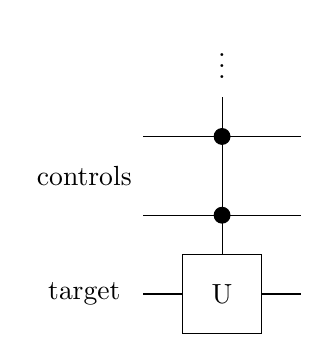
\begin{tikzpicture}[scale=.5] \node[draw=none] at (-3.5, 3) {controls}; \node[draw=none] at (-3.5, 0) {target}; \node[draw=none] at (0, 6) {$\vdots$}; \draw (0, 5) -- (0, 4); \draw (-2, 4) -- (2, 4); \draw[fill=black] (0, 4) circle (.2); \draw (0, 4) -- (0, 2); \draw (-2, 2) -- (2, 2); \draw[fill=black] (0, 2) circle (.2); \draw (0, 2) -- (0, 1); \draw (-2,0) -- (-1, 0); \draw (1, 0) -- (2, 0); \draw (-1,-1)--(-1,1)--(1,1)--(1,-1)--cycle; \node[draw=none] at (0, 0) {U}; \end{tikzpicture} } \]


\begin{DoxyParams}[1]{Parameters}
\mbox{\tt in,out}  & {\em multi\+Qubit} & object representing the set of all qubits \\
\hline
\mbox{\tt in}  & {\em control\+Qubits} & applies unitary if all qubits in this array equal 1 \\
\hline
\mbox{\tt in}  & {\em num\+Control\+Qubits} & number of control qubits \\
\hline
\mbox{\tt in}  & {\em target\+Qubit} & qubit to operate on \\
\hline
\mbox{\tt in}  & {\em u} & single-\/qubit unitary matrix to apply \\
\hline
\end{DoxyParams}

\begin{DoxyExceptions}{Exceptions}
{\em exit\+With\+Error} & if {\ttfamily num\+Control\+Qubits} is outside \mbox{[}1, {\ttfamily multi\+Qubit.\+num\+Qubits}\mbox{]}), or if any qubit index ({\ttfamily target\+Qubit} or one in {\ttfamily control\+Qubits}) is outside \mbox{[}0, {\ttfamily multi\+Qubit.\+num\+Qubits}\mbox{]}), or if {\ttfamily control\+Qubits} contains {\ttfamily target\+Qubit}, or if {\ttfamily u} is not unitary. \\
\hline
\end{DoxyExceptions}


Definition at line 441 of file Qu\+E\+S\+T\+\_\+env\+\_\+mpi.\+c.



References Multi\+Qubit\+::chunk\+Id, chunk\+Is\+Upper(), exchange\+State\+Vectors(), get\+Chunk\+Pair\+Id(), get\+Rot\+Angle\+From\+Unitary\+Matrix(), half\+Matrix\+Block\+Fits\+In\+Chunk(), multi\+Controlled\+Unitary\+Distributed(), multi\+Controlled\+Unitary\+Local(), Multi\+Qubit\+::num\+Amps\+Per\+Chunk, Multi\+Qubit\+::num\+Qubits, Multi\+Qubit\+::pair\+State\+Vec, Qu\+E\+S\+T\+Assert(), Multi\+Qubit\+::state\+Vec, and validate\+Matrix\+Is\+Unitary().


\begin{DoxyCode}
442 \{
443     \mbox{\hyperlink{QuEST__env__mpi_8c_a3587b9d533e633ccf1abf9ad2ce45d8d}{QuESTAssert}}(targetQubit >= 0 && targetQubit < multiQubit.
      \mbox{\hyperlink{structMultiQubit_ab5b9795bdc6fb5855e1974dcbbaeb36f}{numQubits}}, 1, \_\_func\_\_);
444     \mbox{\hyperlink{QuEST__env__mpi_8c_a3587b9d533e633ccf1abf9ad2ce45d8d}{QuESTAssert}}(numControlQubits > 0 && numControlQubits <= multiQubit.
      \mbox{\hyperlink{structMultiQubit_ab5b9795bdc6fb5855e1974dcbbaeb36f}{numQubits}}, 4, \_\_func\_\_);
445     \mbox{\hyperlink{QuEST__env__mpi_8c_a3587b9d533e633ccf1abf9ad2ce45d8d}{QuESTAssert}}(\mbox{\hyperlink{QuEST_8c_ae4fea133d1a8f09ff8da03038100adb2}{validateMatrixIsUnitary}}(u), 5, \_\_func\_\_);
446 
447     \textcolor{keywordtype}{long} \textcolor{keywordtype}{long} \textcolor{keywordtype}{int} mask=0;
448     \textcolor{keywordflow}{for} (\textcolor{keywordtype}{int} i=0; i<numControlQubits; i++) mask = mask | (1LL<<controlQubits[i]);
449     \mbox{\hyperlink{QuEST__env__mpi_8c_a3587b9d533e633ccf1abf9ad2ce45d8d}{QuESTAssert}}(mask >=0 && mask <= (1LL<<multiQubit.\mbox{\hyperlink{structMultiQubit_ab5b9795bdc6fb5855e1974dcbbaeb36f}{numQubits}})-1, 2, \_\_func\_\_);
450     \mbox{\hyperlink{QuEST__env__mpi_8c_a3587b9d533e633ccf1abf9ad2ce45d8d}{QuESTAssert}}((mask & (1LL<<targetQubit)) != (1LL<<targetQubit), 3, \_\_func\_\_);
451 
452     \textcolor{comment}{// flag to require memory exchange. 1: an entire block fits on one rank, 0: at most half a block fits
       on one rank}
453     \textcolor{keywordtype}{int} useLocalDataOnly = \mbox{\hyperlink{QuEST__env__mpi_8c_a4d043bb0cee54a5f94faf3ffc34a6790}{halfMatrixBlockFitsInChunk}}(multiQubit.
      \mbox{\hyperlink{structMultiQubit_a1cad83601a78635dd278259c7ed54f18}{numAmpsPerChunk}}, targetQubit);
454     \mbox{\hyperlink{structComplex}{Complex}} rot1, rot2;
455 
456     \textcolor{comment}{// rank's chunk is in upper half of block }
457     \textcolor{keywordtype}{int} rankIsUpper;
458     \textcolor{keywordtype}{int} pairRank; \textcolor{comment}{// rank of corresponding chunk}
459 
460     \textcolor{keywordflow}{if} (useLocalDataOnly)\{
461         \textcolor{comment}{// all values required to update state vector lie in this rank}
462         \mbox{\hyperlink{QuEST_8c_a1309eabcba3cb97fbc3cd2e606d17766}{multiControlledUnitaryLocal}}(multiQubit, targetQubit, mask, u);
463     \} \textcolor{keywordflow}{else} \{
464         \textcolor{comment}{// need to get corresponding chunk of state vector from other rank}
465         rankIsUpper = \mbox{\hyperlink{QuEST__env__mpi_8c_a0552889d6f57d9e0ed8b209bf426482d}{chunkIsUpper}}(multiQubit.\mbox{\hyperlink{structMultiQubit_ab10c88249fa3825d6227ceec01d37e37}{chunkId}}, multiQubit.
      \mbox{\hyperlink{structMultiQubit_a1cad83601a78635dd278259c7ed54f18}{numAmpsPerChunk}}, targetQubit);
466         \mbox{\hyperlink{QuEST__env__mpi_8c_a5c9b2f129bdffaaba9857f6eddecbb17}{getRotAngleFromUnitaryMatrix}}(rankIsUpper, &rot1, &rot2, u);
467         pairRank = \mbox{\hyperlink{QuEST__env__mpi_8c_a7dba097f23f5d48dfdc9f3250444e2e4}{getChunkPairId}}(rankIsUpper, multiQubit.\mbox{\hyperlink{structMultiQubit_ab10c88249fa3825d6227ceec01d37e37}{chunkId}}, multiQubit.
      \mbox{\hyperlink{structMultiQubit_a1cad83601a78635dd278259c7ed54f18}{numAmpsPerChunk}}, targetQubit);
468         \textcolor{comment}{//printf("%d rank has pair rank: %d\(\backslash\)n", multiQubit.rank, pairRank);}
469         \textcolor{comment}{// get corresponding values from my pair}
470         \mbox{\hyperlink{QuEST__env__mpi_8c_a7682c9a3fd592d34ec15ba8fa172f104}{exchangeStateVectors}}(multiQubit, pairRank);
471 
472         \textcolor{comment}{// this rank's values are either in the upper of lower half of the block. send values to
       multiControlledUnitaryDistributed}
473         \textcolor{comment}{// in the correct order}
474         \textcolor{keywordflow}{if} (rankIsUpper)\{
475             \mbox{\hyperlink{QuEST_8c_a9dbf856ebeea0cf0a3ee5aae6782f2d2}{multiControlledUnitaryDistributed}}(multiQubit,targetQubit,mask,
      rot1,rot2,
476                     multiQubit.\mbox{\hyperlink{structMultiQubit_a45483190d6b01ef6b2f98f2bec9ab94f}{stateVec}}, \textcolor{comment}{//upper}
477                     multiQubit.\mbox{\hyperlink{structMultiQubit_a76f7db4eab52d2b30f58f973ada809c5}{pairStateVec}}, \textcolor{comment}{//lower}
478                     multiQubit.\mbox{\hyperlink{structMultiQubit_a45483190d6b01ef6b2f98f2bec9ab94f}{stateVec}}); \textcolor{comment}{//output}
479         \} \textcolor{keywordflow}{else} \{
480             \mbox{\hyperlink{QuEST_8c_a9dbf856ebeea0cf0a3ee5aae6782f2d2}{multiControlledUnitaryDistributed}}(multiQubit,targetQubit,mask,
      rot1,rot2,
481                     multiQubit.\mbox{\hyperlink{structMultiQubit_a76f7db4eab52d2b30f58f973ada809c5}{pairStateVec}}, \textcolor{comment}{//upper}
482                     multiQubit.\mbox{\hyperlink{structMultiQubit_a45483190d6b01ef6b2f98f2bec9ab94f}{stateVec}}, \textcolor{comment}{//lower}
483                     multiQubit.\mbox{\hyperlink{structMultiQubit_a45483190d6b01ef6b2f98f2bec9ab94f}{stateVec}}); \textcolor{comment}{//output}
484         \}
485     \}
486 \}
\end{DoxyCode}
\mbox{\Hypertarget{QuEST__env__mpi_8c_aae7a8a7f1ccbddb7f76b6c52b746bb43}\label{QuEST__env__mpi_8c_aae7a8a7f1ccbddb7f76b6c52b746bb43}} 
\index{Qu\+E\+S\+T\+\_\+env\+\_\+mpi.\+c@{Qu\+E\+S\+T\+\_\+env\+\_\+mpi.\+c}!phase\+Gate@{phase\+Gate}}
\index{phase\+Gate@{phase\+Gate}!Qu\+E\+S\+T\+\_\+env\+\_\+mpi.\+c@{Qu\+E\+S\+T\+\_\+env\+\_\+mpi.\+c}}
\paragraph{\texorpdfstring{phase\+Gate()}{phaseGate()}}
{\footnotesize\ttfamily void phase\+Gate (\begin{DoxyParamCaption}\item[{\mbox{\hyperlink{structMultiQubit}{Multi\+Qubit}}}]{multi\+Qubit,  }\item[{const int}]{target\+Qubit,  }\item[{enum \mbox{\hyperlink{QuEST_8h_a5739021c733cecc49647956b2f7338ea}{phase\+Gate\+Type}}}]{type }\end{DoxyParamCaption})}



Definition at line 584 of file Qu\+E\+S\+T\+\_\+env\+\_\+mpi.\+c.



References Multi\+Qubit\+::chunk\+Id, chunk\+Is\+Upper(), half\+Matrix\+Block\+Fits\+In\+Chunk(), Multi\+Qubit\+::num\+Amps\+Per\+Chunk, Multi\+Qubit\+::num\+Qubits, phase\+Gate\+Distributed(), phase\+Gate\+Local(), and Qu\+E\+S\+T\+Assert().


\begin{DoxyCode}
585 \{
586     \mbox{\hyperlink{QuEST__env__mpi_8c_a3587b9d533e633ccf1abf9ad2ce45d8d}{QuESTAssert}}(targetQubit >= 0 && targetQubit < multiQubit.
      \mbox{\hyperlink{structMultiQubit_ab5b9795bdc6fb5855e1974dcbbaeb36f}{numQubits}}, 1, \_\_func\_\_);
587 
588     \textcolor{comment}{// flag to require memory exchange. 1: an entire block fits on one rank, 0: at most half a block fits
       on one rank}
589     \textcolor{keywordtype}{int} useLocalDataOnly = \mbox{\hyperlink{QuEST__env__mpi_8c_a4d043bb0cee54a5f94faf3ffc34a6790}{halfMatrixBlockFitsInChunk}}(multiQubit.
      \mbox{\hyperlink{structMultiQubit_a1cad83601a78635dd278259c7ed54f18}{numAmpsPerChunk}}, targetQubit);
590 
591     \textcolor{comment}{// rank's chunk is in upper half of block }
592     \textcolor{keywordtype}{int} rankIsUpper;
593 
594     \textcolor{keywordflow}{if} (useLocalDataOnly)\{
595         \mbox{\hyperlink{QuEST_8c_a3a54566b73ac84c312d7da4f56ffbc3b}{phaseGateLocal}}(multiQubit, targetQubit, type);
596     \} \textcolor{keywordflow}{else} \{
597         rankIsUpper = \mbox{\hyperlink{QuEST__env__mpi_8c_a0552889d6f57d9e0ed8b209bf426482d}{chunkIsUpper}}(multiQubit.\mbox{\hyperlink{structMultiQubit_ab10c88249fa3825d6227ceec01d37e37}{chunkId}}, multiQubit.
      \mbox{\hyperlink{structMultiQubit_a1cad83601a78635dd278259c7ed54f18}{numAmpsPerChunk}}, targetQubit);
598         \textcolor{keywordflow}{if} (!rankIsUpper) \mbox{\hyperlink{QuEST_8c_af832ed00b02a0597b7fe0b714032c54a}{phaseGateDistributed}}(multiQubit, targetQubit, type);
599     \}
600 \}
\end{DoxyCode}
\mbox{\Hypertarget{QuEST__env__mpi_8c_a3587b9d533e633ccf1abf9ad2ce45d8d}\label{QuEST__env__mpi_8c_a3587b9d533e633ccf1abf9ad2ce45d8d}} 
\index{Qu\+E\+S\+T\+\_\+env\+\_\+mpi.\+c@{Qu\+E\+S\+T\+\_\+env\+\_\+mpi.\+c}!Qu\+E\+S\+T\+Assert@{Qu\+E\+S\+T\+Assert}}
\index{Qu\+E\+S\+T\+Assert@{Qu\+E\+S\+T\+Assert}!Qu\+E\+S\+T\+\_\+env\+\_\+mpi.\+c@{Qu\+E\+S\+T\+\_\+env\+\_\+mpi.\+c}}
\paragraph{\texorpdfstring{Qu\+E\+S\+T\+Assert()}{QuESTAssert()}}
{\footnotesize\ttfamily void Qu\+E\+S\+T\+Assert (\begin{DoxyParamCaption}\item[{int}]{is\+Valid,  }\item[{int}]{error\+Code,  }\item[{const char $\ast$}]{func }\end{DoxyParamCaption})}



Definition at line 760 of file Qu\+E\+S\+T\+\_\+env\+\_\+mpi.\+c.



References exit\+With\+Error().



Referenced by collapse\+To\+Outcome(), compact\+Unitary(), controlled\+Compact\+Unitary(), controlled\+Not(), controlled\+Unitary(), find\+Probability\+Of\+Outcome(), hadamard(), measure(), measure\+With\+Stats(), multi\+Controlled\+Unitary(), phase\+Gate(), sigma\+X(), sigma\+Y(), and unitary().


\begin{DoxyCode}
760                                                               \{
761     \textcolor{keywordflow}{if} (!isValid) \mbox{\hyperlink{QuEST__env__mpi_8c_ae5f9019826f35e8b51b1716cfe397b45}{exitWithError}}(errorCode, func);
762 \}
\end{DoxyCode}
\mbox{\Hypertarget{QuEST__env__mpi_8c_a62da5b58d8ce84e6f4d24be1b872294e}\label{QuEST__env__mpi_8c_a62da5b58d8ce84e6f4d24be1b872294e}} 
\index{Qu\+E\+S\+T\+\_\+env\+\_\+mpi.\+c@{Qu\+E\+S\+T\+\_\+env\+\_\+mpi.\+c}!report\+Node\+List@{report\+Node\+List}}
\index{report\+Node\+List@{report\+Node\+List}!Qu\+E\+S\+T\+\_\+env\+\_\+mpi.\+c@{Qu\+E\+S\+T\+\_\+env\+\_\+mpi.\+c}}
\paragraph{\texorpdfstring{report\+Node\+List()}{reportNodeList()}}
{\footnotesize\ttfamily void report\+Node\+List (\begin{DoxyParamCaption}\item[{\mbox{\hyperlink{structQuESTEnv}{Qu\+E\+S\+T\+Env}}}]{env }\end{DoxyParamCaption})}



Report a list of C\+PU hostnames and the rank that is running on each if running with M\+PI enabled and an error message otherwise. 

For debugging purposes. 
\begin{DoxyParams}[1]{Parameters}
\mbox{\tt in}  & {\em env} & object representing the execution environment. A single instance is used for each program \\
\hline
\end{DoxyParams}


Definition at line 82 of file Qu\+E\+S\+T\+\_\+env\+\_\+mpi.\+c.



References env, and Qu\+E\+S\+T\+Env\+::rank.


\begin{DoxyCode}
82                                  \{
83     \textcolor{keywordtype}{char} hostName[256];
84     gethostname(hostName, 255);
85     printf(\textcolor{stringliteral}{"hostname on rank %d: %s\(\backslash\)n"}, \mbox{\hyperlink{runTests_8c_a5fd8ba97fcae3408ae6221dfc3cc1f93}{env}}.\mbox{\hyperlink{structQuESTEnv_aa648bb336cf8598467cb62db00b9cee8}{rank}}, hostName);
86 \}
\end{DoxyCode}
\mbox{\Hypertarget{QuEST__env__mpi_8c_af8a14ae79c3fb2c0b5f6255cc37bebf9}\label{QuEST__env__mpi_8c_af8a14ae79c3fb2c0b5f6255cc37bebf9}} 
\index{Qu\+E\+S\+T\+\_\+env\+\_\+mpi.\+c@{Qu\+E\+S\+T\+\_\+env\+\_\+mpi.\+c}!report\+Qu\+E\+S\+T\+Env@{report\+Qu\+E\+S\+T\+Env}}
\index{report\+Qu\+E\+S\+T\+Env@{report\+Qu\+E\+S\+T\+Env}!Qu\+E\+S\+T\+\_\+env\+\_\+mpi.\+c@{Qu\+E\+S\+T\+\_\+env\+\_\+mpi.\+c}}
\paragraph{\texorpdfstring{report\+Qu\+E\+S\+T\+Env()}{reportQuESTEnv()}}
{\footnotesize\ttfamily void report\+Qu\+E\+S\+T\+Env (\begin{DoxyParamCaption}\item[{\mbox{\hyperlink{structQuESTEnv}{Qu\+E\+S\+T\+Env}}}]{env }\end{DoxyParamCaption})}



Report information about the Qu\+E\+ST environment. 


\begin{DoxyParams}[1]{Parameters}
\mbox{\tt in}  & {\em env} & object representing the execution environment. A single instance is used for each program \\
\hline
\end{DoxyParams}


Definition at line 67 of file Qu\+E\+S\+T\+\_\+env\+\_\+mpi.\+c.



References env, Qu\+E\+S\+T\+Env\+::num\+Ranks, Qu\+E\+S\+T\+Env\+::rank, and R\+E\+AL.


\begin{DoxyCode}
67                                  \{
68     \textcolor{keywordflow}{if} (\mbox{\hyperlink{runTests_8c_a5fd8ba97fcae3408ae6221dfc3cc1f93}{env}}.\mbox{\hyperlink{structQuESTEnv_aa648bb336cf8598467cb62db00b9cee8}{rank}}==0)\{
69         printf(\textcolor{stringliteral}{"EXECUTION ENVIRONMENT:\(\backslash\)n"}); 
70         printf(\textcolor{stringliteral}{"Running distributed (MPI) version\(\backslash\)n"});
71         printf(\textcolor{stringliteral}{"Number of ranks is %d\(\backslash\)n"}, \mbox{\hyperlink{runTests_8c_a5fd8ba97fcae3408ae6221dfc3cc1f93}{env}}.\mbox{\hyperlink{structQuESTEnv_af22aacd7c9905accae28484785c193b4}{numRanks}});
72 \textcolor{preprocessor}{# ifdef \_OPENMP}
73         printf(\textcolor{stringliteral}{"OpenMP enabled\(\backslash\)n"});
74         printf(\textcolor{stringliteral}{"Number of threads available is %d\(\backslash\)n"}, omp\_get\_max\_threads());
75 \textcolor{preprocessor}{# else}
76         printf(\textcolor{stringliteral}{"OpenMP disabled\(\backslash\)n"});
77 \textcolor{preprocessor}{# endif }
78         printf(\textcolor{stringliteral}{"Precision: size of REAL is %ld bytes\(\backslash\)n"}, \textcolor{keyword}{sizeof}(\mbox{\hyperlink{QuEST__precision_8h_a4b654506f18b8bfd61ad2a29a7e38c25}{REAL}}));
79     \}
80 \}
\end{DoxyCode}
\mbox{\Hypertarget{QuEST__env__mpi_8c_a86e396e06b7d527cac20ba0108872423}\label{QuEST__env__mpi_8c_a86e396e06b7d527cac20ba0108872423}} 
\index{Qu\+E\+S\+T\+\_\+env\+\_\+mpi.\+c@{Qu\+E\+S\+T\+\_\+env\+\_\+mpi.\+c}!sigmaX@{sigmaX}}
\index{sigmaX@{sigmaX}!Qu\+E\+S\+T\+\_\+env\+\_\+mpi.\+c@{Qu\+E\+S\+T\+\_\+env\+\_\+mpi.\+c}}
\paragraph{\texorpdfstring{sigma\+X()}{sigmaX()}}
{\footnotesize\ttfamily void sigmaX (\begin{DoxyParamCaption}\item[{\mbox{\hyperlink{structMultiQubit}{Multi\+Qubit}}}]{multi\+Qubit,  }\item[{const int}]{target\+Qubit }\end{DoxyParamCaption})}



Apply the single-\/qubit sigma-\/X (also known as the X, Pauli-\/X, N\+OT or bit-\/flip) gate. 

This is a rotation of $\pi$ around the x-\/axis on the Bloch sphere. I.\+e. \[ \begin{pmatrix} 0 & 1 \\ 1 & 0 \end{pmatrix} \] ~\newline
 \[ \setlength{\fboxrule}{0.01pt} \fbox{ 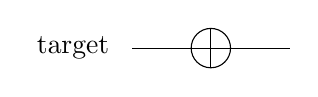
\begin{tikzpicture}[scale=.5] \node[draw=none] at (-3.5, 0) {target}; \draw (-2,0) -- (2, 0); \draw (0, 0) circle (.5); \draw (0, .5) -- (0, -.5); \end{tikzpicture} } \] ~\newline
 
\begin{DoxyParams}[1]{Parameters}
\mbox{\tt in,out}  & {\em multi\+Qubit} & object representing the set of all qubits \\
\hline
\mbox{\tt in}  & {\em target\+Qubit} & qubit to operate on \\
\hline
\end{DoxyParams}

\begin{DoxyExceptions}{Exceptions}
{\em exit\+With\+Error} & if {\ttfamily target\+Qubit} is outside \mbox{[}0, {\ttfamily multi\+Qubit.\+num\+Qubits}). \\
\hline
\end{DoxyExceptions}


Definition at line 487 of file Qu\+E\+S\+T\+\_\+env\+\_\+mpi.\+c.



References Multi\+Qubit\+::chunk\+Id, chunk\+Is\+Upper(), exchange\+State\+Vectors(), get\+Chunk\+Pair\+Id(), half\+Matrix\+Block\+Fits\+In\+Chunk(), Multi\+Qubit\+::num\+Amps\+Per\+Chunk, Multi\+Qubit\+::num\+Qubits, Multi\+Qubit\+::pair\+State\+Vec, Qu\+E\+S\+T\+Assert(), sigma\+X\+Distributed(), sigma\+X\+Local(), and Multi\+Qubit\+::state\+Vec.


\begin{DoxyCode}
488 \{
489     \mbox{\hyperlink{QuEST__env__mpi_8c_a3587b9d533e633ccf1abf9ad2ce45d8d}{QuESTAssert}}(targetQubit >= 0 && targetQubit < multiQubit.
      \mbox{\hyperlink{structMultiQubit_ab5b9795bdc6fb5855e1974dcbbaeb36f}{numQubits}}, 1, \_\_func\_\_);
490 
491     \textcolor{comment}{// flag to require memory exchange. 1: an entire block fits on one rank, 0: at most half a block fits
       on one rank}
492     \textcolor{keywordtype}{int} useLocalDataOnly = \mbox{\hyperlink{QuEST__env__mpi_8c_a4d043bb0cee54a5f94faf3ffc34a6790}{halfMatrixBlockFitsInChunk}}(multiQubit.
      \mbox{\hyperlink{structMultiQubit_a1cad83601a78635dd278259c7ed54f18}{numAmpsPerChunk}}, targetQubit);
493 
494     \textcolor{comment}{// rank's chunk is in upper half of block }
495     \textcolor{keywordtype}{int} rankIsUpper;
496     \textcolor{keywordtype}{int} pairRank; \textcolor{comment}{// rank of corresponding chunk}
497 
498     \textcolor{keywordflow}{if} (useLocalDataOnly)\{
499         \textcolor{comment}{// all values required to update state vector lie in this rank}
500         \mbox{\hyperlink{QuEST_8c_a74822fd86bb5d81766e6e8dbdcd62df1}{sigmaXLocal}}(multiQubit, targetQubit);
501     \} \textcolor{keywordflow}{else} \{
502         \textcolor{comment}{// need to get corresponding chunk of state vector from other rank}
503         rankIsUpper = \mbox{\hyperlink{QuEST__env__mpi_8c_a0552889d6f57d9e0ed8b209bf426482d}{chunkIsUpper}}(multiQubit.\mbox{\hyperlink{structMultiQubit_ab10c88249fa3825d6227ceec01d37e37}{chunkId}}, multiQubit.
      \mbox{\hyperlink{structMultiQubit_a1cad83601a78635dd278259c7ed54f18}{numAmpsPerChunk}}, targetQubit);
504         pairRank = \mbox{\hyperlink{QuEST__env__mpi_8c_a7dba097f23f5d48dfdc9f3250444e2e4}{getChunkPairId}}(rankIsUpper, multiQubit.\mbox{\hyperlink{structMultiQubit_ab10c88249fa3825d6227ceec01d37e37}{chunkId}}, multiQubit.
      \mbox{\hyperlink{structMultiQubit_a1cad83601a78635dd278259c7ed54f18}{numAmpsPerChunk}}, targetQubit);
505         \textcolor{comment}{//printf("%d rank has pair rank: %d\(\backslash\)n", multiQubit.rank, pairRank);}
506         \textcolor{comment}{// get corresponding values from my pair}
507         \mbox{\hyperlink{QuEST__env__mpi_8c_a7682c9a3fd592d34ec15ba8fa172f104}{exchangeStateVectors}}(multiQubit, pairRank);
508         \textcolor{comment}{// this rank's values are either in the upper of lower half of the block. sigmaX just replaces}
509         \textcolor{comment}{// this rank's values with pair values}
510         \mbox{\hyperlink{QuEST_8c_a2275fff50824fe47485890ff5a857785}{sigmaXDistributed}}(multiQubit, targetQubit,
511                 multiQubit.\mbox{\hyperlink{structMultiQubit_a76f7db4eab52d2b30f58f973ada809c5}{pairStateVec}}, \textcolor{comment}{// in}
512                 multiQubit.\mbox{\hyperlink{structMultiQubit_a45483190d6b01ef6b2f98f2bec9ab94f}{stateVec}}); \textcolor{comment}{// out}
513     \}
514 \}
\end{DoxyCode}
\mbox{\Hypertarget{QuEST__env__mpi_8c_a1f54d70a42403f7e1c2e2c2007332f61}\label{QuEST__env__mpi_8c_a1f54d70a42403f7e1c2e2c2007332f61}} 
\index{Qu\+E\+S\+T\+\_\+env\+\_\+mpi.\+c@{Qu\+E\+S\+T\+\_\+env\+\_\+mpi.\+c}!sigmaY@{sigmaY}}
\index{sigmaY@{sigmaY}!Qu\+E\+S\+T\+\_\+env\+\_\+mpi.\+c@{Qu\+E\+S\+T\+\_\+env\+\_\+mpi.\+c}}
\paragraph{\texorpdfstring{sigma\+Y()}{sigmaY()}}
{\footnotesize\ttfamily void sigmaY (\begin{DoxyParamCaption}\item[{\mbox{\hyperlink{structMultiQubit}{Multi\+Qubit}}}]{multi\+Qubit,  }\item[{const int}]{target\+Qubit }\end{DoxyParamCaption})}



Apply the single-\/qubit sigma-\/Y (also known as the Y or Pauli-\/Y) gate. 

This is a rotation of $\pi$ around the Y-\/axis on the Bloch sphere. I.\+e. \[ \begin{pmatrix} 0 & -i \\ i & 0 \end{pmatrix} \] ~\newline
 \[ \setlength{\fboxrule}{0.01pt} \fbox{ 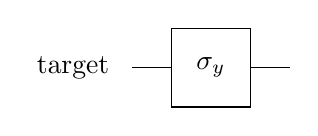
\begin{tikzpicture}[scale=.5] \node[draw=none] at (-3.5, 0) {target}; \draw (-2,0) -- (-1, 0); \draw (1, 0) -- (2, 0); \draw (-1,-1)--(-1,1)--(1,1)--(1,-1)--cycle; \node[draw=none] at (0, 0) {$\sigma_y$}; \end{tikzpicture} } \] ~\newline
 
\begin{DoxyParams}[1]{Parameters}
\mbox{\tt in,out}  & {\em multi\+Qubit} & object representing the set of all qubits \\
\hline
\mbox{\tt in}  & {\em target\+Qubit} & qubit to operate on \\
\hline
\end{DoxyParams}

\begin{DoxyExceptions}{Exceptions}
{\em exit\+With\+Error} & if {\ttfamily target\+Qubit} is outside \mbox{[}0, {\ttfamily multi\+Qubit.\+num\+Qubits}). \\
\hline
\end{DoxyExceptions}
fix -- put duplicate code (sigmaX, sigmaY) in seperate function 

Definition at line 553 of file Qu\+E\+S\+T\+\_\+env\+\_\+mpi.\+c.



References Multi\+Qubit\+::chunk\+Id, chunk\+Is\+Upper(), exchange\+State\+Vectors(), get\+Chunk\+Pair\+Id(), half\+Matrix\+Block\+Fits\+In\+Chunk(), Multi\+Qubit\+::num\+Amps\+Per\+Chunk, Multi\+Qubit\+::num\+Qubits, Multi\+Qubit\+::pair\+State\+Vec, Qu\+E\+S\+T\+Assert(), sigma\+Y\+Distributed(), sigma\+Y\+Local(), and Multi\+Qubit\+::state\+Vec.


\begin{DoxyCode}
554 \{
555     \mbox{\hyperlink{QuEST__env__mpi_8c_a3587b9d533e633ccf1abf9ad2ce45d8d}{QuESTAssert}}(targetQubit >= 0 && targetQubit < multiQubit.
      \mbox{\hyperlink{structMultiQubit_ab5b9795bdc6fb5855e1974dcbbaeb36f}{numQubits}}, 1, \_\_func\_\_);
556 
557     \textcolor{comment}{// flag to require memory exchange. 1: an entire block fits on one rank, 0: at most half a block fits
       on one rank}
558     \textcolor{keywordtype}{int} useLocalDataOnly = \mbox{\hyperlink{QuEST__env__mpi_8c_a4d043bb0cee54a5f94faf3ffc34a6790}{halfMatrixBlockFitsInChunk}}(multiQubit.
      \mbox{\hyperlink{structMultiQubit_a1cad83601a78635dd278259c7ed54f18}{numAmpsPerChunk}}, targetQubit);
559 
560     \textcolor{comment}{// rank's chunk is in upper half of block }
561     \textcolor{keywordtype}{int} rankIsUpper;
562     \textcolor{keywordtype}{int} pairRank; \textcolor{comment}{// rank of corresponding chunk}
563 
564     \textcolor{keywordflow}{if} (useLocalDataOnly)\{
565         \textcolor{comment}{// all values required to update state vector lie in this rank}
566         \mbox{\hyperlink{QuEST_8c_a81fbfaed65a742a7dfd622e17652245e}{sigmaYLocal}}(multiQubit, targetQubit);
567     \} \textcolor{keywordflow}{else} \{
569         \textcolor{comment}{// need to get corresponding chunk of state vector from other rank}
570         rankIsUpper = \mbox{\hyperlink{QuEST__env__mpi_8c_a0552889d6f57d9e0ed8b209bf426482d}{chunkIsUpper}}(multiQubit.\mbox{\hyperlink{structMultiQubit_ab10c88249fa3825d6227ceec01d37e37}{chunkId}}, multiQubit.
      \mbox{\hyperlink{structMultiQubit_a1cad83601a78635dd278259c7ed54f18}{numAmpsPerChunk}}, targetQubit);
571         pairRank = \mbox{\hyperlink{QuEST__env__mpi_8c_a7dba097f23f5d48dfdc9f3250444e2e4}{getChunkPairId}}(rankIsUpper, multiQubit.\mbox{\hyperlink{structMultiQubit_ab10c88249fa3825d6227ceec01d37e37}{chunkId}}, multiQubit.
      \mbox{\hyperlink{structMultiQubit_a1cad83601a78635dd278259c7ed54f18}{numAmpsPerChunk}}, targetQubit);
572         \textcolor{comment}{//printf("%d rank has pair rank: %d\(\backslash\)n", multiQubit.rank, pairRank);}
573         \textcolor{comment}{// get corresponding values from my pair}
574         \mbox{\hyperlink{QuEST__env__mpi_8c_a7682c9a3fd592d34ec15ba8fa172f104}{exchangeStateVectors}}(multiQubit, pairRank);
575         \textcolor{comment}{// this rank's values are either in the upper of lower half of the block. sigmaX just replaces}
576         \textcolor{comment}{// this rank's values with pair values}
577         \mbox{\hyperlink{QuEST_8c_af5ef5166f00c0572354b4ac53dcf40cf}{sigmaYDistributed}}(multiQubit,targetQubit,
578                 multiQubit.\mbox{\hyperlink{structMultiQubit_a76f7db4eab52d2b30f58f973ada809c5}{pairStateVec}}, \textcolor{comment}{// in}
579                 multiQubit.\mbox{\hyperlink{structMultiQubit_a45483190d6b01ef6b2f98f2bec9ab94f}{stateVec}}, \textcolor{comment}{// out}
580                 rankIsUpper);
581     \}
582 \}
\end{DoxyCode}
\mbox{\Hypertarget{QuEST__env__mpi_8c_a8d31fe2d1ad4d01e2a1f5f6b8bc15b77}\label{QuEST__env__mpi_8c_a8d31fe2d1ad4d01e2a1f5f6b8bc15b77}} 
\index{Qu\+E\+S\+T\+\_\+env\+\_\+mpi.\+c@{Qu\+E\+S\+T\+\_\+env\+\_\+mpi.\+c}!sync\+Qu\+E\+S\+T\+Env@{sync\+Qu\+E\+S\+T\+Env}}
\index{sync\+Qu\+E\+S\+T\+Env@{sync\+Qu\+E\+S\+T\+Env}!Qu\+E\+S\+T\+\_\+env\+\_\+mpi.\+c@{Qu\+E\+S\+T\+\_\+env\+\_\+mpi.\+c}}
\paragraph{\texorpdfstring{sync\+Qu\+E\+S\+T\+Env()}{syncQuESTEnv()}}
{\footnotesize\ttfamily void sync\+Qu\+E\+S\+T\+Env (\begin{DoxyParamCaption}\item[{\mbox{\hyperlink{structQuESTEnv}{Qu\+E\+S\+T\+Env}}}]{env }\end{DoxyParamCaption})}



Guarantees that all code up to the given point has been executed on all nodes (if running in distributed mode) 


\begin{DoxyParams}[1]{Parameters}
\mbox{\tt in}  & {\em env} & object representing the execution environment. A single instance is used for each program \\
\hline
\end{DoxyParams}


Definition at line 50 of file Qu\+E\+S\+T\+\_\+env\+\_\+mpi.\+c.


\begin{DoxyCode}
50                                \{
51     MPI\_Barrier(MPI\_COMM\_WORLD);
52 \}
\end{DoxyCode}
\mbox{\Hypertarget{QuEST__env__mpi_8c_ac7e38d768a1bd79019f88cc1e6295092}\label{QuEST__env__mpi_8c_ac7e38d768a1bd79019f88cc1e6295092}} 
\index{Qu\+E\+S\+T\+\_\+env\+\_\+mpi.\+c@{Qu\+E\+S\+T\+\_\+env\+\_\+mpi.\+c}!sync\+Qu\+E\+S\+T\+Success@{sync\+Qu\+E\+S\+T\+Success}}
\index{sync\+Qu\+E\+S\+T\+Success@{sync\+Qu\+E\+S\+T\+Success}!Qu\+E\+S\+T\+\_\+env\+\_\+mpi.\+c@{Qu\+E\+S\+T\+\_\+env\+\_\+mpi.\+c}}
\paragraph{\texorpdfstring{sync\+Qu\+E\+S\+T\+Success()}{syncQuESTSuccess()}}
{\footnotesize\ttfamily int sync\+Qu\+E\+S\+T\+Success (\begin{DoxyParamCaption}\item[{int}]{success\+Code }\end{DoxyParamCaption})}



Performs a logical A\+ND on all success\+Codes held by all processes. 

If any one process has a zero success\+Code all processes will return a zero success code.


\begin{DoxyParams}[1]{Parameters}
\mbox{\tt in}  & {\em env} & object representing the execution environment. A single instance is used for each program \\
\hline
\mbox{\tt in}  & {\em success\+Code} & 1 if process task succeeded, 0 if process task failed \\
\hline
\end{DoxyParams}
\begin{DoxyReturn}{Returns}
1 if all processes succeeded, 0 if any one process failed 
\end{DoxyReturn}


Definition at line 54 of file Qu\+E\+S\+T\+\_\+env\+\_\+mpi.\+c.


\begin{DoxyCode}
54                                      \{
55     \textcolor{keywordtype}{int} totalSuccess;
56     MPI\_Allreduce(&successCode, &totalSuccess, 1, MPI\_INT, MPI\_LAND, MPI\_COMM\_WORLD);
57     \textcolor{keywordflow}{return} totalSuccess;
58 \}
\end{DoxyCode}
\mbox{\Hypertarget{QuEST__env__mpi_8c_a7a0877e33700f6bad48adb51b7b3fb67}\label{QuEST__env__mpi_8c_a7a0877e33700f6bad48adb51b7b3fb67}} 
\index{Qu\+E\+S\+T\+\_\+env\+\_\+mpi.\+c@{Qu\+E\+S\+T\+\_\+env\+\_\+mpi.\+c}!unitary@{unitary}}
\index{unitary@{unitary}!Qu\+E\+S\+T\+\_\+env\+\_\+mpi.\+c@{Qu\+E\+S\+T\+\_\+env\+\_\+mpi.\+c}}
\paragraph{\texorpdfstring{unitary()}{unitary()}}
{\footnotesize\ttfamily void unitary (\begin{DoxyParamCaption}\item[{\mbox{\hyperlink{structMultiQubit}{Multi\+Qubit}}}]{multi\+Qubit,  }\item[{const int}]{target\+Qubit,  }\item[{\mbox{\hyperlink{structComplexMatrix2}{Complex\+Matrix2}}}]{u }\end{DoxyParamCaption})}



Apply a general single-\/qubit unitary (including a global phase factor). 

The passed 2x2 Complex\+Matrix must be unitary, otherwise an error is thrown.

\[ \setlength{\fboxrule}{0.01pt} \fbox{ \begin{tikzpicture}[scale=.5] \node[draw=none] at (-3.5, 0) {target}; \draw (-2,0) -- (-1, 0); \draw (1, 0) -- (2, 0); \draw (-1,-1)--(-1,1)--(1,1)--(1,-1)--cycle; \node[draw=none] at (0, 0) {U}; \end{tikzpicture} } \]


\begin{DoxyParams}[1]{Parameters}
\mbox{\tt in,out}  & {\em multi\+Qubit} & object representing the set of all qubits \\
\hline
\mbox{\tt in}  & {\em target\+Qubit} & qubit to operate on \\
\hline
\mbox{\tt in}  & {\em u} & unitary matrix to apply \\
\hline
\end{DoxyParams}

\begin{DoxyExceptions}{Exceptions}
{\em exit\+With\+Error} & if {\ttfamily target\+Qubit} is outside \mbox{[}0, {\ttfamily multi\+Qubit.\+num\+Qubits}), or matrix {\ttfamily u} is not unitary. \\
\hline
\end{DoxyExceptions}


Definition at line 312 of file Qu\+E\+S\+T\+\_\+env\+\_\+mpi.\+c.



References Multi\+Qubit\+::chunk\+Id, chunk\+Is\+Upper(), exchange\+State\+Vectors(), get\+Chunk\+Pair\+Id(), get\+Rot\+Angle\+From\+Unitary\+Matrix(), half\+Matrix\+Block\+Fits\+In\+Chunk(), Multi\+Qubit\+::num\+Amps\+Per\+Chunk, Multi\+Qubit\+::num\+Qubits, Multi\+Qubit\+::pair\+State\+Vec, Qu\+E\+S\+T\+Assert(), Multi\+Qubit\+::state\+Vec, unitary\+Distributed(), unitary\+Local(), and validate\+Matrix\+Is\+Unitary().


\begin{DoxyCode}
313 \{
314     \mbox{\hyperlink{QuEST__env__mpi_8c_a3587b9d533e633ccf1abf9ad2ce45d8d}{QuESTAssert}}(targetQubit >= 0 && targetQubit < multiQubit.
      \mbox{\hyperlink{structMultiQubit_ab5b9795bdc6fb5855e1974dcbbaeb36f}{numQubits}}, 1, \_\_func\_\_);
315     \mbox{\hyperlink{QuEST__env__mpi_8c_a3587b9d533e633ccf1abf9ad2ce45d8d}{QuESTAssert}}(\mbox{\hyperlink{QuEST_8c_ae4fea133d1a8f09ff8da03038100adb2}{validateMatrixIsUnitary}}(u), 5, \_\_func\_\_);
316 
317     \textcolor{comment}{// flag to require memory exchange. 1: an entire block fits on one rank, 0: at most half a block fits
       on one rank}
318     \textcolor{keywordtype}{int} useLocalDataOnly = \mbox{\hyperlink{QuEST__env__mpi_8c_a4d043bb0cee54a5f94faf3ffc34a6790}{halfMatrixBlockFitsInChunk}}(multiQubit.
      \mbox{\hyperlink{structMultiQubit_a1cad83601a78635dd278259c7ed54f18}{numAmpsPerChunk}}, targetQubit);
319     \mbox{\hyperlink{structComplex}{Complex}} rot1, rot2;
320 
321     \textcolor{comment}{// rank's chunk is in upper half of block }
322     \textcolor{keywordtype}{int} rankIsUpper;
323     \textcolor{keywordtype}{int} pairRank; \textcolor{comment}{// rank of corresponding chunk}
324 
325     \textcolor{keywordflow}{if} (useLocalDataOnly)\{
326         \textcolor{comment}{// all values required to update state vector lie in this rank}
327         \mbox{\hyperlink{QuEST_8c_ac134fb45b0a7248c5d15e16eb7139a35}{unitaryLocal}}(multiQubit, targetQubit, u);
328     \} \textcolor{keywordflow}{else} \{
329         \textcolor{comment}{// need to get corresponding chunk of state vector from other rank}
330         rankIsUpper = \mbox{\hyperlink{QuEST__env__mpi_8c_a0552889d6f57d9e0ed8b209bf426482d}{chunkIsUpper}}(multiQubit.\mbox{\hyperlink{structMultiQubit_ab10c88249fa3825d6227ceec01d37e37}{chunkId}}, multiQubit.
      \mbox{\hyperlink{structMultiQubit_a1cad83601a78635dd278259c7ed54f18}{numAmpsPerChunk}}, targetQubit);
331         \mbox{\hyperlink{QuEST__env__mpi_8c_a5c9b2f129bdffaaba9857f6eddecbb17}{getRotAngleFromUnitaryMatrix}}(rankIsUpper, &rot1, &rot2, u);
332         pairRank = \mbox{\hyperlink{QuEST__env__mpi_8c_a7dba097f23f5d48dfdc9f3250444e2e4}{getChunkPairId}}(rankIsUpper, multiQubit.\mbox{\hyperlink{structMultiQubit_ab10c88249fa3825d6227ceec01d37e37}{chunkId}}, multiQubit.
      \mbox{\hyperlink{structMultiQubit_a1cad83601a78635dd278259c7ed54f18}{numAmpsPerChunk}}, targetQubit);
333         \textcolor{comment}{// get corresponding values from my pair}
334         \mbox{\hyperlink{QuEST__env__mpi_8c_a7682c9a3fd592d34ec15ba8fa172f104}{exchangeStateVectors}}(multiQubit, pairRank);
335 
336         \textcolor{comment}{// this rank's values are either in the upper of lower half of the block. }
337         \textcolor{comment}{// send values to compactUnitaryDistributed in the correct order}
338         \textcolor{keywordflow}{if} (rankIsUpper)\{
339             \mbox{\hyperlink{QuEST_8c_a2343b7240118e89aa615e2c9140b770b}{unitaryDistributed}}(multiQubit,targetQubit,rot1,rot2,
340                     multiQubit.\mbox{\hyperlink{structMultiQubit_a45483190d6b01ef6b2f98f2bec9ab94f}{stateVec}}, \textcolor{comment}{//upper}
341                     multiQubit.\mbox{\hyperlink{structMultiQubit_a76f7db4eab52d2b30f58f973ada809c5}{pairStateVec}}, \textcolor{comment}{//lower}
342                     multiQubit.\mbox{\hyperlink{structMultiQubit_a45483190d6b01ef6b2f98f2bec9ab94f}{stateVec}}); \textcolor{comment}{//output}
343         \} \textcolor{keywordflow}{else} \{
344             \mbox{\hyperlink{QuEST_8c_a2343b7240118e89aa615e2c9140b770b}{unitaryDistributed}}(multiQubit,targetQubit,rot1,rot2,
345                     multiQubit.\mbox{\hyperlink{structMultiQubit_a76f7db4eab52d2b30f58f973ada809c5}{pairStateVec}}, \textcolor{comment}{//upper}
346                     multiQubit.\mbox{\hyperlink{structMultiQubit_a45483190d6b01ef6b2f98f2bec9ab94f}{stateVec}}, \textcolor{comment}{//lower}
347                     multiQubit.\mbox{\hyperlink{structMultiQubit_a45483190d6b01ef6b2f98f2bec9ab94f}{stateVec}}); \textcolor{comment}{//output}
348         \}
349     \}
350 
351 
352 \}
\end{DoxyCode}

\hypertarget{QuEST__internal_8h}{}\subsection{Qu\+E\+S\+T\+\_\+internal.\+h File Reference}
\label{QuEST__internal_8h}\index{Qu\+E\+S\+T\+\_\+internal.\+h@{Qu\+E\+S\+T\+\_\+internal.\+h}}


Internal functions used to implement the public facing A\+PI in qubits.\+h.  


{\ttfamily \#include \char`\"{}Qu\+E\+S\+T\+\_\+precision.\+h\char`\"{}}\newline
\subsubsection*{Functions}
\begin{DoxyCompactItemize}
\item 
\mbox{\hyperlink{QuEST__precision_8h_a4b654506f18b8bfd61ad2a29a7e38c25}{R\+E\+AL}} \mbox{\hyperlink{QuEST__internal_8h_a7a1f63ec3c42d9ad72f1f01c14a885db}{collapse\+To\+Outcome\+Distributed\+Renorm}} (\mbox{\hyperlink{structMultiQubit}{Multi\+Qubit}} multi\+Qubit, const int measure\+Qubit, const \mbox{\hyperlink{QuEST__precision_8h_a4b654506f18b8bfd61ad2a29a7e38c25}{R\+E\+AL}} total\+Probability)
\begin{DoxyCompactList}\small\item\em Renormalise parts of the state vector where measure\+Qubit=0 or 1, based on the total probability of that qubit being in state 0 or 1. \end{DoxyCompactList}\item 
void \mbox{\hyperlink{QuEST__internal_8h_a78908fe8e75a21fd4f7fa7dff05d6be1}{collapse\+To\+Outcome\+Distributed\+Set\+Zero}} (\mbox{\hyperlink{structMultiQubit}{Multi\+Qubit}} multi\+Qubit, const int measure\+Qubit)
\begin{DoxyCompactList}\small\item\em Set all amplitudes in one chunk to 0. \end{DoxyCompactList}\item 
void \mbox{\hyperlink{QuEST__internal_8h_a01d9a8b7ff0e09ec399e158389783aa9}{collapse\+To\+Outcome\+Local}} (\mbox{\hyperlink{structMultiQubit}{Multi\+Qubit}} multi\+Qubit, int measure\+Qubit, \mbox{\hyperlink{QuEST__precision_8h_a4b654506f18b8bfd61ad2a29a7e38c25}{R\+E\+AL}} total\+Probability, int outcome)
\begin{DoxyCompactList}\small\item\em Update the state vector to be consistent with measuring measure\+Qubit=0 if outcome=0 and measure\+Qubit=1 if outcome=1. \end{DoxyCompactList}\item 
void \mbox{\hyperlink{QuEST__internal_8h_a20ee1878a63ae6112e8845f4a8787592}{compact\+Unitary\+Distributed}} (\mbox{\hyperlink{structMultiQubit}{Multi\+Qubit}} multi\+Qubit, const int target\+Qubit, \mbox{\hyperlink{structComplex}{Complex}} rot1, \mbox{\hyperlink{structComplex}{Complex}} rot2, \mbox{\hyperlink{structComplexArray}{Complex\+Array}} state\+Vec\+Up, \mbox{\hyperlink{structComplexArray}{Complex\+Array}} state\+Vec\+Lo, \mbox{\hyperlink{structComplexArray}{Complex\+Array}} state\+Vec\+Out)
\begin{DoxyCompactList}\small\item\em Rotate a single qubit in the state vector of probability amplitudes, given two complex numbers alpha and beta, and a subset of the state vector with upper and lower block values stored seperately. \end{DoxyCompactList}\item 
void \mbox{\hyperlink{QuEST__internal_8h_a9cee2d8716667a3318420a3b672f5b92}{compact\+Unitary\+Local}} (\mbox{\hyperlink{structMultiQubit}{Multi\+Qubit}} multi\+Qubit, const int target\+Qubit, \mbox{\hyperlink{structComplex}{Complex}} alpha, \mbox{\hyperlink{structComplex}{Complex}} beta)
\item 
void \mbox{\hyperlink{QuEST__internal_8h_a717855e835e3161e08c18cdc15325d27}{controlled\+Compact\+Unitary\+Distributed}} (\mbox{\hyperlink{structMultiQubit}{Multi\+Qubit}} multi\+Qubit, const int control\+Qubit, const int target\+Qubit, \mbox{\hyperlink{structComplex}{Complex}} rot1, \mbox{\hyperlink{structComplex}{Complex}} rot2, \mbox{\hyperlink{structComplexArray}{Complex\+Array}} state\+Vec\+Up, \mbox{\hyperlink{structComplexArray}{Complex\+Array}} state\+Vec\+Lo, \mbox{\hyperlink{structComplexArray}{Complex\+Array}} state\+Vec\+Out)
\begin{DoxyCompactList}\small\item\em Rotate a single qubit in the state vector of probability amplitudes, given two complex numbers alpha and beta and a subset of the state vector with upper and lower block values stored seperately. \end{DoxyCompactList}\item 
void \mbox{\hyperlink{QuEST__internal_8h_afc77657651d52c47403b44b923a098a8}{controlled\+Compact\+Unitary\+Local}} (\mbox{\hyperlink{structMultiQubit}{Multi\+Qubit}} multi\+Qubit, const int control\+Qubit, const int target\+Qubit, \mbox{\hyperlink{structComplex}{Complex}} alpha, \mbox{\hyperlink{structComplex}{Complex}} beta)
\item 
void \mbox{\hyperlink{QuEST__internal_8h_a05875a70b539a3efb28d027823403f34}{controlled\+Not\+Distributed}} (\mbox{\hyperlink{structMultiQubit}{Multi\+Qubit}} multi\+Qubit, const int control\+Qubit, const int target\+Qubit, \mbox{\hyperlink{structComplexArray}{Complex\+Array}} state\+Vec\+In, \mbox{\hyperlink{structComplexArray}{Complex\+Array}} state\+Vec\+Out)
\begin{DoxyCompactList}\small\item\em Rotate a single qubit by \{\{0,1\},\{1,0\}. \end{DoxyCompactList}\item 
void \mbox{\hyperlink{QuEST__internal_8h_ad357a43e80e3baf013975b1b70942f4c}{controlled\+Not\+Local}} (\mbox{\hyperlink{structMultiQubit}{Multi\+Qubit}} multi\+Qubit, const int control\+Qubit, const int target\+Qubit)
\item 
void \mbox{\hyperlink{QuEST__internal_8h_a642093063a1f889f61a1311f6d6f2d3f}{controlled\+Unitary\+Distributed}} (\mbox{\hyperlink{structMultiQubit}{Multi\+Qubit}} multi\+Qubit, const int control\+Qubit, const int target\+Qubit, \mbox{\hyperlink{structComplex}{Complex}} rot1, \mbox{\hyperlink{structComplex}{Complex}} rot2, \mbox{\hyperlink{structComplexArray}{Complex\+Array}} state\+Vec\+Up, \mbox{\hyperlink{structComplexArray}{Complex\+Array}} state\+Vec\+Lo, \mbox{\hyperlink{structComplexArray}{Complex\+Array}} state\+Vec\+Out)
\begin{DoxyCompactList}\small\item\em Rotate a single qubit in the state vector of probability amplitudes, given two complex numbers alpha and beta and a subset of the state vector with upper and lower block values stored seperately. \end{DoxyCompactList}\item 
void \mbox{\hyperlink{QuEST__internal_8h_a8a4afcff70195a306c082b8ed8d4e09a}{controlled\+Unitary\+Local}} (\mbox{\hyperlink{structMultiQubit}{Multi\+Qubit}} multi\+Qubit, const int control\+Qubit, const int target\+Qubit, \mbox{\hyperlink{structComplexMatrix2}{Complex\+Matrix2}} u)
\item 
void \mbox{\hyperlink{QuEST__internal_8h_ae5f9019826f35e8b51b1716cfe397b45}{exit\+With\+Error}} (int error\+Code, const char $\ast$func)
\item 
\mbox{\hyperlink{QuEST__precision_8h_a4b654506f18b8bfd61ad2a29a7e38c25}{R\+E\+AL}} \mbox{\hyperlink{QuEST__internal_8h_a9ac9bb717a889f09d307eda9f0b65957}{find\+Probability\+Of\+Zero\+Distributed}} (\mbox{\hyperlink{structMultiQubit}{Multi\+Qubit}} multi\+Qubit, const int measure\+Qubit)
\begin{DoxyCompactList}\small\item\em Measure the probability of a specified qubit being in the zero state across all amplitudes held in this chunk. \end{DoxyCompactList}\item 
\mbox{\hyperlink{QuEST__precision_8h_a4b654506f18b8bfd61ad2a29a7e38c25}{R\+E\+AL}} \mbox{\hyperlink{QuEST__internal_8h_a7c02cd0e1b4eac19771a0525f023249e}{find\+Probability\+Of\+Zero\+Local}} (\mbox{\hyperlink{structMultiQubit}{Multi\+Qubit}} multi\+Qubit, const int measure\+Qubit)
\begin{DoxyCompactList}\small\item\em Measure the total probability of a specified qubit being in the zero state across all amplitudes in this chunk. \end{DoxyCompactList}\item 
void \mbox{\hyperlink{QuEST__internal_8h_ae6a897066979fc52d977007d959ca09d}{hadamard\+Distributed}} (\mbox{\hyperlink{structMultiQubit}{Multi\+Qubit}} multi\+Qubit, const int target\+Qubit, \mbox{\hyperlink{structComplexArray}{Complex\+Array}} state\+Vec\+Up, \mbox{\hyperlink{structComplexArray}{Complex\+Array}} state\+Vec\+Lo, \mbox{\hyperlink{structComplexArray}{Complex\+Array}} state\+Vec\+Out, int update\+Upper)
\begin{DoxyCompactList}\small\item\em Rotate a single qubit by \{\{1,1\},\{1,-\/1\}\}/sqrt2. \end{DoxyCompactList}\item 
void \mbox{\hyperlink{QuEST__internal_8h_aa9f0718b4dd794a3e1b143e3b153bfc5}{hadamard\+Local}} (\mbox{\hyperlink{structMultiQubit}{Multi\+Qubit}} multi\+Qubit, const int target\+Qubit)
\item 
unsigned long int \mbox{\hyperlink{QuEST__internal_8h_ab76254cfde16f0808476649507a1a2fc}{hash\+String}} (char $\ast$str)
\item 
void \mbox{\hyperlink{QuEST__internal_8h_a9dbf856ebeea0cf0a3ee5aae6782f2d2}{multi\+Controlled\+Unitary\+Distributed}} (\mbox{\hyperlink{structMultiQubit}{Multi\+Qubit}} multi\+Qubit, const int target\+Qubit, long long int mask, \mbox{\hyperlink{structComplex}{Complex}} rot1, \mbox{\hyperlink{structComplex}{Complex}} rot2, \mbox{\hyperlink{structComplexArray}{Complex\+Array}} state\+Vec\+Up, \mbox{\hyperlink{structComplexArray}{Complex\+Array}} state\+Vec\+Lo, \mbox{\hyperlink{structComplexArray}{Complex\+Array}} state\+Vec\+Out)
\begin{DoxyCompactList}\small\item\em Apply a unitary operation to a single qubit in the state vector of probability amplitudes, given a subset of the state vector with upper and lower block values stored seperately. \end{DoxyCompactList}\item 
void \mbox{\hyperlink{QuEST__internal_8h_a1309eabcba3cb97fbc3cd2e606d17766}{multi\+Controlled\+Unitary\+Local}} (\mbox{\hyperlink{structMultiQubit}{Multi\+Qubit}} multi\+Qubit, const int target\+Qubit, long long int mask, \mbox{\hyperlink{structComplexMatrix2}{Complex\+Matrix2}} u)
\item 
void \mbox{\hyperlink{QuEST__internal_8h_aae7a8a7f1ccbddb7f76b6c52b746bb43}{phase\+Gate}} (\mbox{\hyperlink{structMultiQubit}{Multi\+Qubit}} multi\+Qubit, const int target\+Qubit, enum \mbox{\hyperlink{QuEST_8h_a5739021c733cecc49647956b2f7338ea}{phase\+Gate\+Type}} type)
\item 
void \mbox{\hyperlink{QuEST__internal_8h_af832ed00b02a0597b7fe0b714032c54a}{phase\+Gate\+Distributed}} (\mbox{\hyperlink{structMultiQubit}{Multi\+Qubit}} multi\+Qubit, const int target\+Qubit, enum \mbox{\hyperlink{QuEST_8h_a5739021c733cecc49647956b2f7338ea}{phase\+Gate\+Type}} type)
\item 
void \mbox{\hyperlink{QuEST__internal_8h_a3a54566b73ac84c312d7da4f56ffbc3b}{phase\+Gate\+Local}} (\mbox{\hyperlink{structMultiQubit}{Multi\+Qubit}} multi\+Qubit, const int target\+Qubit, enum \mbox{\hyperlink{QuEST_8h_a5739021c733cecc49647956b2f7338ea}{phase\+Gate\+Type}} type)
\item 
void \mbox{\hyperlink{QuEST__internal_8h_a3587b9d533e633ccf1abf9ad2ce45d8d}{Qu\+E\+S\+T\+Assert}} (int is\+Valid, int error\+Code, const char $\ast$func)
\item 
void \mbox{\hyperlink{QuEST__internal_8h_a2275fff50824fe47485890ff5a857785}{sigma\+X\+Distributed}} (\mbox{\hyperlink{structMultiQubit}{Multi\+Qubit}} multi\+Qubit, const int target\+Qubit, \mbox{\hyperlink{structComplexArray}{Complex\+Array}} state\+Vec\+In, \mbox{\hyperlink{structComplexArray}{Complex\+Array}} state\+Vec\+Out)
\begin{DoxyCompactList}\small\item\em Rotate a single qubit by \{\{0,1\},\{1,0\}. \end{DoxyCompactList}\item 
void \mbox{\hyperlink{QuEST__internal_8h_a74822fd86bb5d81766e6e8dbdcd62df1}{sigma\+X\+Local}} (\mbox{\hyperlink{structMultiQubit}{Multi\+Qubit}} multi\+Qubit, const int target\+Qubit)
\item 
void \mbox{\hyperlink{QuEST__internal_8h_af5ef5166f00c0572354b4ac53dcf40cf}{sigma\+Y\+Distributed}} (\mbox{\hyperlink{structMultiQubit}{Multi\+Qubit}} multi\+Qubit, const int target\+Qubit, \mbox{\hyperlink{structComplexArray}{Complex\+Array}} state\+Vec\+In, \mbox{\hyperlink{structComplexArray}{Complex\+Array}} state\+Vec\+Out, int update\+Upper)
\begin{DoxyCompactList}\small\item\em Rotate a single qubit by \{\{0,-\/i\},\{i,0\}. \end{DoxyCompactList}\item 
void \mbox{\hyperlink{QuEST__internal_8h_a81fbfaed65a742a7dfd622e17652245e}{sigma\+Y\+Local}} (\mbox{\hyperlink{structMultiQubit}{Multi\+Qubit}} multi\+Qubit, const int target\+Qubit)
\item 
void \mbox{\hyperlink{QuEST__internal_8h_a2343b7240118e89aa615e2c9140b770b}{unitary\+Distributed}} (\mbox{\hyperlink{structMultiQubit}{Multi\+Qubit}} multi\+Qubit, const int target\+Qubit, \mbox{\hyperlink{structComplex}{Complex}} rot1, \mbox{\hyperlink{structComplex}{Complex}} rot2, \mbox{\hyperlink{structComplexArray}{Complex\+Array}} state\+Vec\+Up, \mbox{\hyperlink{structComplexArray}{Complex\+Array}} state\+Vec\+Lo, \mbox{\hyperlink{structComplexArray}{Complex\+Array}} state\+Vec\+Out)
\begin{DoxyCompactList}\small\item\em Apply a unitary operation to a single qubit given a subset of the state vector with upper and lower block values stored seperately. \end{DoxyCompactList}\item 
void \mbox{\hyperlink{QuEST__internal_8h_ac134fb45b0a7248c5d15e16eb7139a35}{unitary\+Local}} (\mbox{\hyperlink{structMultiQubit}{Multi\+Qubit}} multi\+Qubit, const int target\+Qubit, \mbox{\hyperlink{structComplexMatrix2}{Complex\+Matrix2}} u)
\item 
int \mbox{\hyperlink{QuEST__internal_8h_ae2b2c14a07dd7d50ff86032a3ca101d7}{validate\+Alpha\+Beta}} (\mbox{\hyperlink{structComplex}{Complex}} alpha, \mbox{\hyperlink{structComplex}{Complex}} beta)
\item 
int \mbox{\hyperlink{QuEST__internal_8h_ae4fea133d1a8f09ff8da03038100adb2}{validate\+Matrix\+Is\+Unitary}} (\mbox{\hyperlink{structComplexMatrix2}{Complex\+Matrix2}} u)
\item 
int \mbox{\hyperlink{QuEST__internal_8h_a71c14976f63cfcda70026fa20ee531fe}{validate\+Unit\+Vector}} (\mbox{\hyperlink{QuEST__precision_8h_a4b654506f18b8bfd61ad2a29a7e38c25}{R\+E\+AL}} ux, \mbox{\hyperlink{QuEST__precision_8h_a4b654506f18b8bfd61ad2a29a7e38c25}{R\+E\+AL}} uy, \mbox{\hyperlink{QuEST__precision_8h_a4b654506f18b8bfd61ad2a29a7e38c25}{R\+E\+AL}} uz)
\end{DoxyCompactItemize}
\subsubsection*{Variables}
\begin{DoxyCompactItemize}
\item 
const char $\ast$ \mbox{\hyperlink{QuEST__internal_8h_aac1637696885c75b73a1ecf381cea713}{error\+Codes}} \mbox{[}$\,$\mbox{]}
\end{DoxyCompactItemize}


\subsubsection{Detailed Description}
Internal functions used to implement the public facing A\+PI in qubits.\+h. 

Do not call these functions directly. In general, qubits\+\_\+env\+\_\+local.\+c and qubits\+\_\+env\+\_\+mpi.\+c will implement the public A\+PI by choosing the correct function or combination of functions to use from those included here. 

\subsubsection{Function Documentation}
\mbox{\Hypertarget{QuEST__internal_8h_a7a1f63ec3c42d9ad72f1f01c14a885db}\label{QuEST__internal_8h_a7a1f63ec3c42d9ad72f1f01c14a885db}} 
\index{Qu\+E\+S\+T\+\_\+internal.\+h@{Qu\+E\+S\+T\+\_\+internal.\+h}!collapse\+To\+Outcome\+Distributed\+Renorm@{collapse\+To\+Outcome\+Distributed\+Renorm}}
\index{collapse\+To\+Outcome\+Distributed\+Renorm@{collapse\+To\+Outcome\+Distributed\+Renorm}!Qu\+E\+S\+T\+\_\+internal.\+h@{Qu\+E\+S\+T\+\_\+internal.\+h}}
\paragraph{\texorpdfstring{collapse\+To\+Outcome\+Distributed\+Renorm()}{collapseToOutcomeDistributedRenorm()}}
{\footnotesize\ttfamily \mbox{\hyperlink{QuEST__precision_8h_a4b654506f18b8bfd61ad2a29a7e38c25}{R\+E\+AL}} collapse\+To\+Outcome\+Distributed\+Renorm (\begin{DoxyParamCaption}\item[{\mbox{\hyperlink{structMultiQubit}{Multi\+Qubit}}}]{multi\+Qubit,  }\item[{const int}]{measure\+Qubit,  }\item[{const \mbox{\hyperlink{QuEST__precision_8h_a4b654506f18b8bfd61ad2a29a7e38c25}{R\+E\+AL}}}]{total\+Probability }\end{DoxyParamCaption})}



Renormalise parts of the state vector where measure\+Qubit=0 or 1, based on the total probability of that qubit being in state 0 or 1. 

Measure in Zero performs an irreversible change to the state vector\+: it updates the vector according to the event that the value \textquotesingle{}outcome\textquotesingle{} has been measured on the qubit indicated by measure\+Qubit (where this label starts from 0, of course). It achieves this by setting all inconsistent amplitudes to 0 and then renormalising based on the total probability of measuring measure\+Qubit=0 if outcome=0 and measure\+Qubit=1 if outcome=1. In the distributed version, one block (with measure\+Qubit=0 in the first half of the block and measure\+Qubit=1 in the second half of the block) is spread over multiple chunks, meaning that each chunks performs only renormalisation or only setting amplitudes to 0. This function handles the renormalisation.


\begin{DoxyParams}[1]{Parameters}
\mbox{\tt in,out}  & {\em multi\+Qubit} & object representing the set of qubits \\
\hline
\mbox{\tt in}  & {\em measure\+Qubit} & qubit to measure \\
\hline
\mbox{\tt in}  & {\em total\+Probability} & probability of qubit measure\+Qubit being zero \\
\hline
\end{DoxyParams}


Definition at line 1922 of file Qu\+E\+S\+T.\+c.



References Complex\+Array\+::imag, Multi\+Qubit\+::num\+Amps\+Divided\+By\+Num\+Chunks, Complex\+Array\+::real, R\+E\+AL, and Multi\+Qubit\+::state\+Vec.



Referenced by collapse\+To\+Outcome(), and measure\+With\+Stats().


\begin{DoxyCode}
1923 \{
1924     \textcolor{comment}{// ----- temp variables}
1925     \textcolor{keywordtype}{long} \textcolor{keywordtype}{long} \textcolor{keywordtype}{int} thisTask;                                   
1926     \textcolor{keywordtype}{long} \textcolor{keywordtype}{long} \textcolor{keywordtype}{int} numTasks=multiQubit.\mbox{\hyperlink{structMultiQubit_a04c9f5254af58e4c4a54712eb32e7082}{numAmpsDividedByNumChunks}};
1927 
1928     \mbox{\hyperlink{QuEST__precision_8h_a4b654506f18b8bfd61ad2a29a7e38c25}{REAL}} renorm=1/sqrt(totalProbability);
1929 
1930     \mbox{\hyperlink{QuEST__precision_8h_a4b654506f18b8bfd61ad2a29a7e38c25}{REAL}} *stateVecReal = multiQubit.\mbox{\hyperlink{structMultiQubit_a45483190d6b01ef6b2f98f2bec9ab94f}{stateVec}}.\mbox{\hyperlink{structComplexArray_a4195cac6c784ea1b6271f1c7dba1548a}{real}};
1931     \mbox{\hyperlink{QuEST__precision_8h_a4b654506f18b8bfd61ad2a29a7e38c25}{REAL}} *stateVecImag = multiQubit.\mbox{\hyperlink{structMultiQubit_a45483190d6b01ef6b2f98f2bec9ab94f}{stateVec}}.\mbox{\hyperlink{structComplexArray_a79dde47c7ae530c79cebfdf57b225968}{imag}};
1932 
1933 \textcolor{preprocessor}{# ifdef \_OPENMP}
1934 \textcolor{preprocessor}{# pragma omp parallel \(\backslash\)}
1935 \textcolor{preprocessor}{    shared    (numTasks,stateVecReal,stateVecImag) \(\backslash\)}
1936 \textcolor{preprocessor}{    private   (thisTask)}
1937 \textcolor{preprocessor}{# endif}
1938     \{
1939 \textcolor{preprocessor}{# ifdef \_OPENMP}
1940 \textcolor{preprocessor}{# pragma omp for schedule  (static)}
1941 \textcolor{preprocessor}{# endif}
1942         \textcolor{keywordflow}{for} (thisTask=0; thisTask<numTasks; thisTask++) \{
1943             stateVecReal[thisTask] = stateVecReal[thisTask]*renorm;
1944             stateVecImag[thisTask] = stateVecImag[thisTask]*renorm;
1945         \}
1946     \}
1947     \textcolor{keywordflow}{return} totalProbability;
1948 \}
\end{DoxyCode}
\mbox{\Hypertarget{QuEST__internal_8h_a78908fe8e75a21fd4f7fa7dff05d6be1}\label{QuEST__internal_8h_a78908fe8e75a21fd4f7fa7dff05d6be1}} 
\index{Qu\+E\+S\+T\+\_\+internal.\+h@{Qu\+E\+S\+T\+\_\+internal.\+h}!collapse\+To\+Outcome\+Distributed\+Set\+Zero@{collapse\+To\+Outcome\+Distributed\+Set\+Zero}}
\index{collapse\+To\+Outcome\+Distributed\+Set\+Zero@{collapse\+To\+Outcome\+Distributed\+Set\+Zero}!Qu\+E\+S\+T\+\_\+internal.\+h@{Qu\+E\+S\+T\+\_\+internal.\+h}}
\paragraph{\texorpdfstring{collapse\+To\+Outcome\+Distributed\+Set\+Zero()}{collapseToOutcomeDistributedSetZero()}}
{\footnotesize\ttfamily void collapse\+To\+Outcome\+Distributed\+Set\+Zero (\begin{DoxyParamCaption}\item[{\mbox{\hyperlink{structMultiQubit}{Multi\+Qubit}}}]{multi\+Qubit,  }\item[{const int}]{measure\+Qubit }\end{DoxyParamCaption})}



Set all amplitudes in one chunk to 0. 

Measure in Zero performs an irreversible change to the state vector\+: it updates the vector according to the event that a zero have been measured on the qubit indicated by measure\+Qubit (where this label starts from 0, of course). It achieves this by setting all inconsistent amplitudes to 0 and then renormalising based on the total probability of measuring measure\+Qubit=0 or 1. In the distributed version, one block (with measure\+Qubit=0 in the first half of the block and measure\+Qubit=1 in the second half of the block) is spread over multiple chunks, meaning that each chunks performs only renormalisation or only setting amplitudes to 0. This function handles setting amplitudes to 0.


\begin{DoxyParams}[1]{Parameters}
\mbox{\tt in,out}  & {\em multi\+Qubit} & object representing the set of qubits \\
\hline
\mbox{\tt in}  & {\em measure\+Qubit} & qubit to measure \\
\hline
\end{DoxyParams}


Definition at line 1962 of file Qu\+E\+S\+T.\+c.



References Complex\+Array\+::imag, Multi\+Qubit\+::num\+Amps\+Divided\+By\+Num\+Chunks, Complex\+Array\+::real, R\+E\+AL, and Multi\+Qubit\+::state\+Vec.



Referenced by collapse\+To\+Outcome(), and measure\+With\+Stats().


\begin{DoxyCode}
1963 \{
1964     \textcolor{comment}{// ----- temp variables}
1965     \textcolor{keywordtype}{long} \textcolor{keywordtype}{long} \textcolor{keywordtype}{int} thisTask;                                   
1966     \textcolor{keywordtype}{long} \textcolor{keywordtype}{long} \textcolor{keywordtype}{int} numTasks=multiQubit.\mbox{\hyperlink{structMultiQubit_a04c9f5254af58e4c4a54712eb32e7082}{numAmpsDividedByNumChunks}};
1967 
1968     \textcolor{comment}{// ---------------------------------------------------------------- //}
1969     \textcolor{comment}{//            find probability                                      //}
1970     \textcolor{comment}{// ---------------------------------------------------------------- //}
1971 
1972     \mbox{\hyperlink{QuEST__precision_8h_a4b654506f18b8bfd61ad2a29a7e38c25}{REAL}} *stateVecReal = multiQubit.\mbox{\hyperlink{structMultiQubit_a45483190d6b01ef6b2f98f2bec9ab94f}{stateVec}}.\mbox{\hyperlink{structComplexArray_a4195cac6c784ea1b6271f1c7dba1548a}{real}};
1973     \mbox{\hyperlink{QuEST__precision_8h_a4b654506f18b8bfd61ad2a29a7e38c25}{REAL}} *stateVecImag = multiQubit.\mbox{\hyperlink{structMultiQubit_a45483190d6b01ef6b2f98f2bec9ab94f}{stateVec}}.\mbox{\hyperlink{structComplexArray_a79dde47c7ae530c79cebfdf57b225968}{imag}};
1974 
1975 \textcolor{preprocessor}{# ifdef \_OPENMP}
1976 \textcolor{preprocessor}{# pragma omp parallel \(\backslash\)}
1977 \textcolor{preprocessor}{    shared    (numTasks,stateVecReal,stateVecImag) \(\backslash\)}
1978 \textcolor{preprocessor}{    private   (thisTask)}
1979 \textcolor{preprocessor}{# endif}
1980     \{
1981 \textcolor{preprocessor}{# ifdef \_OPENMP}
1982 \textcolor{preprocessor}{# pragma omp for schedule  (static)}
1983 \textcolor{preprocessor}{# endif}
1984         \textcolor{keywordflow}{for} (thisTask=0; thisTask<numTasks; thisTask++) \{
1985             stateVecReal[thisTask] = 0;
1986             stateVecImag[thisTask] = 0;
1987         \}
1988     \}
1989 \}
\end{DoxyCode}
\mbox{\Hypertarget{QuEST__internal_8h_a01d9a8b7ff0e09ec399e158389783aa9}\label{QuEST__internal_8h_a01d9a8b7ff0e09ec399e158389783aa9}} 
\index{Qu\+E\+S\+T\+\_\+internal.\+h@{Qu\+E\+S\+T\+\_\+internal.\+h}!collapse\+To\+Outcome\+Local@{collapse\+To\+Outcome\+Local}}
\index{collapse\+To\+Outcome\+Local@{collapse\+To\+Outcome\+Local}!Qu\+E\+S\+T\+\_\+internal.\+h@{Qu\+E\+S\+T\+\_\+internal.\+h}}
\paragraph{\texorpdfstring{collapse\+To\+Outcome\+Local()}{collapseToOutcomeLocal()}}
{\footnotesize\ttfamily void collapse\+To\+Outcome\+Local (\begin{DoxyParamCaption}\item[{\mbox{\hyperlink{structMultiQubit}{Multi\+Qubit}}}]{multi\+Qubit,  }\item[{int}]{measure\+Qubit,  }\item[{\mbox{\hyperlink{QuEST__precision_8h_a4b654506f18b8bfd61ad2a29a7e38c25}{R\+E\+AL}}}]{total\+Probability,  }\item[{int}]{outcome }\end{DoxyParamCaption})}



Update the state vector to be consistent with measuring measure\+Qubit=0 if outcome=0 and measure\+Qubit=1 if outcome=1. 

Performs an irreversible change to the state vector\+: it updates the vector according to the event that an outcome have been measured on the qubit indicated by measure\+Qubit (where this label starts from 0, of course). It achieves this by setting all inconsistent amplitudes to 0 and then renormalising based on the total probability of measuring measure\+Qubit=0 or 1 according to the value of outcome. In the local version, one or more blocks (with measure\+Qubit=0 in the first half of the block and measure\+Qubit=1 in the second half of the block) fit entirely into one chunk.


\begin{DoxyParams}[1]{Parameters}
\mbox{\tt in,out}  & {\em multi\+Qubit} & object representing the set of qubits \\
\hline
\mbox{\tt in}  & {\em measure\+Qubit} & qubit to measure \\
\hline
\mbox{\tt in}  & {\em total\+Probability} & probability of qubit measure\+Qubit being either zero or one \\
\hline
\mbox{\tt in}  & {\em outcome} & to measure the probability of and set the state to -- either zero or one \\
\hline
\end{DoxyParams}


Definition at line 1840 of file Qu\+E\+S\+T.\+c.



References Complex\+Array\+::imag, Multi\+Qubit\+::num\+Amps\+Divided\+By\+Num\+Chunks, Complex\+Array\+::real, R\+E\+AL, and Multi\+Qubit\+::state\+Vec.



Referenced by collapse\+To\+Outcome(), and measure\+With\+Stats().


\begin{DoxyCode}
1841 \{
1842     \textcolor{comment}{// ----- sizes}
1843     \textcolor{keywordtype}{long} \textcolor{keywordtype}{long} \textcolor{keywordtype}{int} sizeBlock,                                  \textcolor{comment}{// size of blocks}
1844          sizeHalfBlock;                                       \textcolor{comment}{// size of blocks halved}
1845     \textcolor{comment}{// ----- indices}
1846     \textcolor{keywordtype}{long} \textcolor{keywordtype}{long} \textcolor{keywordtype}{int} thisBlock,                                  \textcolor{comment}{// current block}
1847          index;                                               \textcolor{comment}{// current index for first half block}
1848     \textcolor{comment}{// ----- measured probability}
1849     \mbox{\hyperlink{QuEST__precision_8h_a4b654506f18b8bfd61ad2a29a7e38c25}{REAL}}   renorm;                                            \textcolor{comment}{// probability (returned) value}
1850     \textcolor{comment}{// ----- temp variables}
1851     \textcolor{keywordtype}{long} \textcolor{keywordtype}{long} \textcolor{keywordtype}{int} thisTask;                                   \textcolor{comment}{// task based approach for expose loop with
       small granularity}
1852     \textcolor{comment}{// (good for shared memory parallelism)}
1853     \textcolor{keywordtype}{long} \textcolor{keywordtype}{long} \textcolor{keywordtype}{int} numTasks=multiQubit.\mbox{\hyperlink{structMultiQubit_a04c9f5254af58e4c4a54712eb32e7082}{numAmpsDividedByNumChunks}}>>1;
1854 
1855     \textcolor{comment}{// ---------------------------------------------------------------- //}
1856     \textcolor{comment}{//            dimensions                                            //}
1857     \textcolor{comment}{// ---------------------------------------------------------------- //}
1858     sizeHalfBlock = 1LL << (measureQubit);                       \textcolor{comment}{// number of state vector elements to sum,}
1859     \textcolor{comment}{// and then the number to skip}
1860     sizeBlock     = 2LL * sizeHalfBlock;                         \textcolor{comment}{// size of blocks (pairs of measure and
       skip entries)}
1861 
1862     renorm=1/sqrt(totalProbability);
1863     \mbox{\hyperlink{QuEST__precision_8h_a4b654506f18b8bfd61ad2a29a7e38c25}{REAL}} *stateVecReal = multiQubit.\mbox{\hyperlink{structMultiQubit_a45483190d6b01ef6b2f98f2bec9ab94f}{stateVec}}.\mbox{\hyperlink{structComplexArray_a4195cac6c784ea1b6271f1c7dba1548a}{real}};
1864     \mbox{\hyperlink{QuEST__precision_8h_a4b654506f18b8bfd61ad2a29a7e38c25}{REAL}} *stateVecImag = multiQubit.\mbox{\hyperlink{structMultiQubit_a45483190d6b01ef6b2f98f2bec9ab94f}{stateVec}}.\mbox{\hyperlink{structComplexArray_a79dde47c7ae530c79cebfdf57b225968}{imag}};
1865 
1866 
1867 \textcolor{preprocessor}{# ifdef \_OPENMP}
1868 \textcolor{preprocessor}{# pragma omp parallel \(\backslash\)}
1869 \textcolor{preprocessor}{    default (none) \(\backslash\)}
1870 \textcolor{preprocessor}{    shared    (numTasks,sizeBlock,sizeHalfBlock, stateVecReal,stateVecImag,renorm,outcome) \(\backslash\)}
1871 \textcolor{preprocessor}{    private   (thisTask,thisBlock,index)}
1872 \textcolor{preprocessor}{# endif}
1873     \{
1874         \textcolor{keywordflow}{if} (outcome==0)\{
1875             \textcolor{comment}{// measure qubit is 0}
1876 \textcolor{preprocessor}{# ifdef \_OPENMP}
1877 \textcolor{preprocessor}{# pragma omp for schedule  (static)}
1878 \textcolor{preprocessor}{# endif}
1879             \textcolor{keywordflow}{for} (thisTask=0; thisTask<numTasks; thisTask++) \{
1880                 thisBlock = thisTask / sizeHalfBlock;
1881                 index     = thisBlock*sizeBlock + thisTask%sizeHalfBlock;
1882                 stateVecReal[index]=stateVecReal[index]*renorm;
1883                 stateVecImag[index]=stateVecImag[index]*renorm;
1884 
1885                 stateVecReal[index+sizeHalfBlock]=0;
1886                 stateVecImag[index+sizeHalfBlock]=0;
1887             \}
1888         \} \textcolor{keywordflow}{else} \{
1889             \textcolor{comment}{// measure qubit is 1}
1890 \textcolor{preprocessor}{# ifdef \_OPENMP}
1891 \textcolor{preprocessor}{# pragma omp for schedule  (static)}
1892 \textcolor{preprocessor}{# endif}
1893             \textcolor{keywordflow}{for} (thisTask=0; thisTask<numTasks; thisTask++) \{
1894                 thisBlock = thisTask / sizeHalfBlock;
1895                 index     = thisBlock*sizeBlock + thisTask%sizeHalfBlock;
1896                 stateVecReal[index]=0;
1897                 stateVecImag[index]=0;
1898 
1899                 stateVecReal[index+sizeHalfBlock]=stateVecReal[index+sizeHalfBlock]*renorm;
1900                 stateVecImag[index+sizeHalfBlock]=stateVecImag[index+sizeHalfBlock]*renorm;
1901             \}
1902         \}
1903     \}
1904 
1905 \}
\end{DoxyCode}
\mbox{\Hypertarget{QuEST__internal_8h_a20ee1878a63ae6112e8845f4a8787592}\label{QuEST__internal_8h_a20ee1878a63ae6112e8845f4a8787592}} 
\index{Qu\+E\+S\+T\+\_\+internal.\+h@{Qu\+E\+S\+T\+\_\+internal.\+h}!compact\+Unitary\+Distributed@{compact\+Unitary\+Distributed}}
\index{compact\+Unitary\+Distributed@{compact\+Unitary\+Distributed}!Qu\+E\+S\+T\+\_\+internal.\+h@{Qu\+E\+S\+T\+\_\+internal.\+h}}
\paragraph{\texorpdfstring{compact\+Unitary\+Distributed()}{compactUnitaryDistributed()}}
{\footnotesize\ttfamily void compact\+Unitary\+Distributed (\begin{DoxyParamCaption}\item[{\mbox{\hyperlink{structMultiQubit}{Multi\+Qubit}}}]{multi\+Qubit,  }\item[{const int}]{target\+Qubit,  }\item[{\mbox{\hyperlink{structComplex}{Complex}}}]{rot1,  }\item[{\mbox{\hyperlink{structComplex}{Complex}}}]{rot2,  }\item[{\mbox{\hyperlink{structComplexArray}{Complex\+Array}}}]{state\+Vec\+Up,  }\item[{\mbox{\hyperlink{structComplexArray}{Complex\+Array}}}]{state\+Vec\+Lo,  }\item[{\mbox{\hyperlink{structComplexArray}{Complex\+Array}}}]{state\+Vec\+Out }\end{DoxyParamCaption})}



Rotate a single qubit in the state vector of probability amplitudes, given two complex numbers alpha and beta, and a subset of the state vector with upper and lower block values stored seperately. 


\begin{DoxyParams}[1]{Parameters}
\mbox{\tt in,out}  & {\em multi\+Qubit} & object representing the set of qubits \\
\hline
\mbox{\tt in}  & {\em target\+Qubit} & qubit to rotate \\
\hline
\mbox{\tt in}  & {\em rot1} & rotation angle \\
\hline
\mbox{\tt in}  & {\em rot2} & rotation angle \\
\hline
\mbox{\tt in}  & {\em state\+Vec\+Up} & probability amplitudes in upper half of a block \\
\hline
\mbox{\tt in}  & {\em state\+Vec\+Lo} & probability amplitudes in lower half of a block \\
\hline
\mbox{\tt out}  & {\em state\+Vec\+Out} & array section to update (will correspond to either the lower or upper half of a block) \\
\hline
\end{DoxyParams}


Definition at line 624 of file Qu\+E\+S\+T.\+c.



References Complex\+Array\+::imag, Complex\+::imag, Multi\+Qubit\+::num\+Amps\+Divided\+By\+Num\+Chunks, Complex\+Array\+::real, R\+E\+AL, and Complex\+::real.



Referenced by compact\+Unitary().


\begin{DoxyCode}
629 \{
630 
631     \mbox{\hyperlink{QuEST__precision_8h_a4b654506f18b8bfd61ad2a29a7e38c25}{REAL}}   stateRealUp,stateRealLo,stateImagUp,stateImagLo;
632     \textcolor{keywordtype}{long} \textcolor{keywordtype}{long} \textcolor{keywordtype}{int} thisTask;  
633     \textcolor{keyword}{const} \textcolor{keywordtype}{long} \textcolor{keywordtype}{long} \textcolor{keywordtype}{int} numTasks=multiQubit.\mbox{\hyperlink{structMultiQubit_a04c9f5254af58e4c4a54712eb32e7082}{numAmpsDividedByNumChunks}};
634 
635     \mbox{\hyperlink{QuEST__precision_8h_a4b654506f18b8bfd61ad2a29a7e38c25}{REAL}} rot1Real=rot1.\mbox{\hyperlink{structComplex_a479ad939835457595fcca3ca55c06283}{real}}, rot1Imag=rot1.\mbox{\hyperlink{structComplex_a1151948284b21c0052f203f23ab931d9}{imag}};
636     \mbox{\hyperlink{QuEST__precision_8h_a4b654506f18b8bfd61ad2a29a7e38c25}{REAL}} rot2Real=rot2.\mbox{\hyperlink{structComplex_a479ad939835457595fcca3ca55c06283}{real}}, rot2Imag=rot2.\mbox{\hyperlink{structComplex_a1151948284b21c0052f203f23ab931d9}{imag}};
637     \mbox{\hyperlink{QuEST__precision_8h_a4b654506f18b8bfd61ad2a29a7e38c25}{REAL}} *stateVecRealUp=stateVecUp.\mbox{\hyperlink{structComplexArray_a4195cac6c784ea1b6271f1c7dba1548a}{real}}, *stateVecImagUp=stateVecUp.
      \mbox{\hyperlink{structComplexArray_a79dde47c7ae530c79cebfdf57b225968}{imag}};
638     \mbox{\hyperlink{QuEST__precision_8h_a4b654506f18b8bfd61ad2a29a7e38c25}{REAL}} *stateVecRealLo=stateVecLo.\mbox{\hyperlink{structComplexArray_a4195cac6c784ea1b6271f1c7dba1548a}{real}}, *stateVecImagLo=stateVecLo.
      \mbox{\hyperlink{structComplexArray_a79dde47c7ae530c79cebfdf57b225968}{imag}};
639     \mbox{\hyperlink{QuEST__precision_8h_a4b654506f18b8bfd61ad2a29a7e38c25}{REAL}} *stateVecRealOut=stateVecOut.\mbox{\hyperlink{structComplexArray_a4195cac6c784ea1b6271f1c7dba1548a}{real}}, *stateVecImagOut=stateVecOut.
      \mbox{\hyperlink{structComplexArray_a79dde47c7ae530c79cebfdf57b225968}{imag}};
640 
641 \textcolor{preprocessor}{# ifdef \_OPENMP}
642 \textcolor{preprocessor}{# pragma omp parallel \(\backslash\)}
643 \textcolor{preprocessor}{    default  (none) \(\backslash\)}
644 \textcolor{preprocessor}{    shared   (stateVecRealUp,stateVecImagUp,stateVecRealLo,stateVecImagLo,stateVecRealOut,stateVecImagOut, 
      \(\backslash\)}
645 \textcolor{preprocessor}{            rot1Real,rot1Imag, rot2Real,rot2Imag) \(\backslash\)}
646 \textcolor{preprocessor}{    private  (thisTask,stateRealUp,stateImagUp,stateRealLo,stateImagLo)}
647 \textcolor{preprocessor}{# endif}
648     \{
649 \textcolor{preprocessor}{# ifdef \_OPENMP}
650 \textcolor{preprocessor}{# pragma omp for schedule (static)}
651 \textcolor{preprocessor}{# endif}
652         \textcolor{keywordflow}{for} (thisTask=0; thisTask<numTasks; thisTask++) \{
653             \textcolor{comment}{// store current state vector values in temp variables}
654             stateRealUp = stateVecRealUp[thisTask];
655             stateImagUp = stateVecImagUp[thisTask];
656 
657             stateRealLo = stateVecRealLo[thisTask];
658             stateImagLo = stateVecImagLo[thisTask];
659 
660             \textcolor{comment}{// state[indexUp] = alpha * state[indexUp] - conj(beta)  * state[indexLo]}
661             stateVecRealOut[thisTask] = rot1Real*stateRealUp - rot1Imag*stateImagUp + rot2Real*stateRealLo 
      + rot2Imag*stateImagLo;
662             stateVecImagOut[thisTask] = rot1Real*stateImagUp + rot1Imag*stateRealUp + rot2Real*stateImagLo 
      - rot2Imag*stateRealLo;
663         \}
664     \}
665 \}
\end{DoxyCode}
\mbox{\Hypertarget{QuEST__internal_8h_a9cee2d8716667a3318420a3b672f5b92}\label{QuEST__internal_8h_a9cee2d8716667a3318420a3b672f5b92}} 
\index{Qu\+E\+S\+T\+\_\+internal.\+h@{Qu\+E\+S\+T\+\_\+internal.\+h}!compact\+Unitary\+Local@{compact\+Unitary\+Local}}
\index{compact\+Unitary\+Local@{compact\+Unitary\+Local}!Qu\+E\+S\+T\+\_\+internal.\+h@{Qu\+E\+S\+T\+\_\+internal.\+h}}
\paragraph{\texorpdfstring{compact\+Unitary\+Local()}{compactUnitaryLocal()}}
{\footnotesize\ttfamily void compact\+Unitary\+Local (\begin{DoxyParamCaption}\item[{\mbox{\hyperlink{structMultiQubit}{Multi\+Qubit}}}]{multi\+Qubit,  }\item[{const int}]{target\+Qubit,  }\item[{\mbox{\hyperlink{structComplex}{Complex}}}]{alpha,  }\item[{\mbox{\hyperlink{structComplex}{Complex}}}]{beta }\end{DoxyParamCaption})}



Definition at line 495 of file Qu\+E\+S\+T.\+c.



References Complex\+Array\+::imag, Complex\+::imag, Multi\+Qubit\+::num\+Amps\+Divided\+By\+Num\+Chunks, Complex\+Array\+::real, R\+E\+AL, Complex\+::real, and Multi\+Qubit\+::state\+Vec.



Referenced by compact\+Unitary().


\begin{DoxyCode}
496 \{
497     \textcolor{keywordtype}{long} \textcolor{keywordtype}{long} \textcolor{keywordtype}{int} sizeBlock, sizeHalfBlock;
498     \textcolor{keywordtype}{long} \textcolor{keywordtype}{long} \textcolor{keywordtype}{int} thisBlock, \textcolor{comment}{// current block}
499          indexUp,indexLo;    \textcolor{comment}{// current index and corresponding index in lower half block}
500 
501     \mbox{\hyperlink{QuEST__precision_8h_a4b654506f18b8bfd61ad2a29a7e38c25}{REAL}} stateRealUp,stateRealLo,stateImagUp,stateImagLo;
502     \textcolor{keywordtype}{long} \textcolor{keywordtype}{long} \textcolor{keywordtype}{int} thisTask;         
503     \textcolor{keyword}{const} \textcolor{keywordtype}{long} \textcolor{keywordtype}{long} \textcolor{keywordtype}{int} numTasks=multiQubit.\mbox{\hyperlink{structMultiQubit_a04c9f5254af58e4c4a54712eb32e7082}{numAmpsDividedByNumChunks}}>>1;
504 
505     \textcolor{comment}{// set dimensions}
506     sizeHalfBlock = 1LL << targetQubit;  
507     sizeBlock     = 2LL * sizeHalfBlock; 
508 
509     \textcolor{comment}{// Can't use multiQubit.stateVec as a private OMP var}
510     \mbox{\hyperlink{QuEST__precision_8h_a4b654506f18b8bfd61ad2a29a7e38c25}{REAL}} *stateVecReal = multiQubit.\mbox{\hyperlink{structMultiQubit_a45483190d6b01ef6b2f98f2bec9ab94f}{stateVec}}.\mbox{\hyperlink{structComplexArray_a4195cac6c784ea1b6271f1c7dba1548a}{real}};
511     \mbox{\hyperlink{QuEST__precision_8h_a4b654506f18b8bfd61ad2a29a7e38c25}{REAL}} *stateVecImag = multiQubit.\mbox{\hyperlink{structMultiQubit_a45483190d6b01ef6b2f98f2bec9ab94f}{stateVec}}.\mbox{\hyperlink{structComplexArray_a79dde47c7ae530c79cebfdf57b225968}{imag}};
512     \mbox{\hyperlink{QuEST__precision_8h_a4b654506f18b8bfd61ad2a29a7e38c25}{REAL}} alphaImag=alpha.\mbox{\hyperlink{structComplex_a1151948284b21c0052f203f23ab931d9}{imag}}, alphaReal=alpha.\mbox{\hyperlink{structComplex_a479ad939835457595fcca3ca55c06283}{real}};
513     \mbox{\hyperlink{QuEST__precision_8h_a4b654506f18b8bfd61ad2a29a7e38c25}{REAL}} betaImag=beta.\mbox{\hyperlink{structComplex_a1151948284b21c0052f203f23ab931d9}{imag}}, betaReal=beta.\mbox{\hyperlink{structComplex_a479ad939835457595fcca3ca55c06283}{real}};
514 
515 \textcolor{preprocessor}{# ifdef \_OPENMP}
516 \textcolor{preprocessor}{# pragma omp parallel \(\backslash\)}
517 \textcolor{preprocessor}{    default  (none) \(\backslash\)}
518 \textcolor{preprocessor}{    shared   (sizeBlock,sizeHalfBlock, stateVecReal,stateVecImag, alphaReal,alphaImag, betaReal,betaImag) \(\backslash\)}
519 \textcolor{preprocessor}{    private  (thisTask,thisBlock ,indexUp,indexLo, stateRealUp,stateImagUp,stateRealLo,stateImagLo) }
520 \textcolor{preprocessor}{# endif}
521     \{
522 \textcolor{preprocessor}{# ifdef \_OPENMP}
523 \textcolor{preprocessor}{# pragma omp for schedule (static)}
524 \textcolor{preprocessor}{# endif}
525         \textcolor{keywordflow}{for} (thisTask=0; thisTask<numTasks; thisTask++) \{
526 
527             thisBlock   = thisTask / sizeHalfBlock;
528             indexUp     = thisBlock*sizeBlock + thisTask%sizeHalfBlock;
529             indexLo     = indexUp + sizeHalfBlock;
530 
531             \textcolor{comment}{// store current state vector values in temp variables}
532             stateRealUp = stateVecReal[indexUp];
533             stateImagUp = stateVecImag[indexUp];
534 
535             stateRealLo = stateVecReal[indexLo];
536             stateImagLo = stateVecImag[indexLo];
537 
538             \textcolor{comment}{// state[indexUp] = alpha * state[indexUp] - conj(beta)  * state[indexLo]}
539             stateVecReal[indexUp] = alphaReal*stateRealUp - alphaImag*stateImagUp 
540                 - betaReal*stateRealLo - betaImag*stateImagLo;
541             stateVecImag[indexUp] = alphaReal*stateImagUp + alphaImag*stateRealUp 
542                 - betaReal*stateImagLo + betaImag*stateRealLo;
543 
544             \textcolor{comment}{// state[indexLo] = beta  * state[indexUp] + conj(alpha) * state[indexLo]}
545             stateVecReal[indexLo] = betaReal*stateRealUp - betaImag*stateImagUp 
546                 + alphaReal*stateRealLo + alphaImag*stateImagLo;
547             stateVecImag[indexLo] = betaReal*stateImagUp + betaImag*stateRealUp 
548                 + alphaReal*stateImagLo - alphaImag*stateRealLo;
549         \} 
550     \}
551 
552 \} 
\end{DoxyCode}
\mbox{\Hypertarget{QuEST__internal_8h_a717855e835e3161e08c18cdc15325d27}\label{QuEST__internal_8h_a717855e835e3161e08c18cdc15325d27}} 
\index{Qu\+E\+S\+T\+\_\+internal.\+h@{Qu\+E\+S\+T\+\_\+internal.\+h}!controlled\+Compact\+Unitary\+Distributed@{controlled\+Compact\+Unitary\+Distributed}}
\index{controlled\+Compact\+Unitary\+Distributed@{controlled\+Compact\+Unitary\+Distributed}!Qu\+E\+S\+T\+\_\+internal.\+h@{Qu\+E\+S\+T\+\_\+internal.\+h}}
\paragraph{\texorpdfstring{controlled\+Compact\+Unitary\+Distributed()}{controlledCompactUnitaryDistributed()}}
{\footnotesize\ttfamily void controlled\+Compact\+Unitary\+Distributed (\begin{DoxyParamCaption}\item[{\mbox{\hyperlink{structMultiQubit}{Multi\+Qubit}}}]{multi\+Qubit,  }\item[{const int}]{control\+Qubit,  }\item[{const int}]{target\+Qubit,  }\item[{\mbox{\hyperlink{structComplex}{Complex}}}]{rot1,  }\item[{\mbox{\hyperlink{structComplex}{Complex}}}]{rot2,  }\item[{\mbox{\hyperlink{structComplexArray}{Complex\+Array}}}]{state\+Vec\+Up,  }\item[{\mbox{\hyperlink{structComplexArray}{Complex\+Array}}}]{state\+Vec\+Lo,  }\item[{\mbox{\hyperlink{structComplexArray}{Complex\+Array}}}]{state\+Vec\+Out }\end{DoxyParamCaption})}



Rotate a single qubit in the state vector of probability amplitudes, given two complex numbers alpha and beta and a subset of the state vector with upper and lower block values stored seperately. 

Only perform the rotation where the control qubit is one.


\begin{DoxyParams}[1]{Parameters}
\mbox{\tt in,out}  & {\em multi\+Qubit} & object representing the set of qubits \\
\hline
\mbox{\tt in}  & {\em target\+Qubit} & qubit to rotate \\
\hline
\mbox{\tt in}  & {\em control\+Qubit} & qubit to determine whether or not to perform a rotation \\
\hline
\mbox{\tt in}  & {\em rot1} & rotation angle \\
\hline
\mbox{\tt in}  & {\em rot2} & rotation angle \\
\hline
\mbox{\tt in}  & {\em state\+Vec\+Up} & probability amplitudes in upper half of a block \\
\hline
\mbox{\tt in}  & {\em state\+Vec\+Lo} & probability amplitudes in lower half of a block \\
\hline
\mbox{\tt out}  & {\em state\+Vec\+Out} & array section to update (will correspond to either the lower or upper half of a block) \\
\hline
\end{DoxyParams}


Definition at line 934 of file Qu\+E\+S\+T.\+c.



References Multi\+Qubit\+::chunk\+Id, extract\+Bit(), Complex\+Array\+::imag, Complex\+::imag, Multi\+Qubit\+::num\+Amps\+Divided\+By\+Num\+Chunks, Complex\+Array\+::real, R\+E\+AL, and Complex\+::real.



Referenced by controlled\+Compact\+Unitary().


\begin{DoxyCode}
939 \{
940 
941     \mbox{\hyperlink{QuEST__precision_8h_a4b654506f18b8bfd61ad2a29a7e38c25}{REAL}}   stateRealUp,stateRealLo,stateImagUp,stateImagLo;
942     \textcolor{keywordtype}{long} \textcolor{keywordtype}{long} \textcolor{keywordtype}{int} thisTask;  
943     \textcolor{keyword}{const} \textcolor{keywordtype}{long} \textcolor{keywordtype}{long} \textcolor{keywordtype}{int} numTasks=multiQubit.\mbox{\hyperlink{structMultiQubit_a04c9f5254af58e4c4a54712eb32e7082}{numAmpsDividedByNumChunks}};
944     \textcolor{keyword}{const} \textcolor{keywordtype}{long} \textcolor{keywordtype}{long} \textcolor{keywordtype}{int} chunkSize=multiQubit.\mbox{\hyperlink{structMultiQubit_a04c9f5254af58e4c4a54712eb32e7082}{numAmpsDividedByNumChunks}};
945     \textcolor{keyword}{const} \textcolor{keywordtype}{long} \textcolor{keywordtype}{long} \textcolor{keywordtype}{int} chunkId=multiQubit.\mbox{\hyperlink{structMultiQubit_ab10c88249fa3825d6227ceec01d37e37}{chunkId}};
946 
947     \textcolor{keywordtype}{int} controlBit;
948 
949     \mbox{\hyperlink{QuEST__precision_8h_a4b654506f18b8bfd61ad2a29a7e38c25}{REAL}} rot1Real=rot1.\mbox{\hyperlink{structComplex_a479ad939835457595fcca3ca55c06283}{real}}, rot1Imag=rot1.\mbox{\hyperlink{structComplex_a1151948284b21c0052f203f23ab931d9}{imag}};
950     \mbox{\hyperlink{QuEST__precision_8h_a4b654506f18b8bfd61ad2a29a7e38c25}{REAL}} rot2Real=rot2.\mbox{\hyperlink{structComplex_a479ad939835457595fcca3ca55c06283}{real}}, rot2Imag=rot2.\mbox{\hyperlink{structComplex_a1151948284b21c0052f203f23ab931d9}{imag}};
951     \mbox{\hyperlink{QuEST__precision_8h_a4b654506f18b8bfd61ad2a29a7e38c25}{REAL}} *stateVecRealUp=stateVecUp.\mbox{\hyperlink{structComplexArray_a4195cac6c784ea1b6271f1c7dba1548a}{real}}, *stateVecImagUp=stateVecUp.
      \mbox{\hyperlink{structComplexArray_a79dde47c7ae530c79cebfdf57b225968}{imag}};
952     \mbox{\hyperlink{QuEST__precision_8h_a4b654506f18b8bfd61ad2a29a7e38c25}{REAL}} *stateVecRealLo=stateVecLo.\mbox{\hyperlink{structComplexArray_a4195cac6c784ea1b6271f1c7dba1548a}{real}}, *stateVecImagLo=stateVecLo.
      \mbox{\hyperlink{structComplexArray_a79dde47c7ae530c79cebfdf57b225968}{imag}};
953     \mbox{\hyperlink{QuEST__precision_8h_a4b654506f18b8bfd61ad2a29a7e38c25}{REAL}} *stateVecRealOut=stateVecOut.\mbox{\hyperlink{structComplexArray_a4195cac6c784ea1b6271f1c7dba1548a}{real}}, *stateVecImagOut=stateVecOut.
      \mbox{\hyperlink{structComplexArray_a79dde47c7ae530c79cebfdf57b225968}{imag}};
954 
955 \textcolor{preprocessor}{# ifdef \_OPENMP}
956 \textcolor{preprocessor}{# pragma omp parallel \(\backslash\)}
957 \textcolor{preprocessor}{    default  (none) \(\backslash\)}
958 \textcolor{preprocessor}{    shared   (stateVecRealUp,stateVecImagUp,stateVecRealLo,stateVecImagLo,stateVecRealOut,stateVecImagOut, 
      \(\backslash\)}
959 \textcolor{preprocessor}{            rot1Real,rot1Imag, rot2Real,rot2Imag) \(\backslash\)}
960 \textcolor{preprocessor}{    private  (thisTask,stateRealUp,stateImagUp,stateRealLo,stateImagLo,controlBit)}
961 \textcolor{preprocessor}{# endif}
962     \{
963 \textcolor{preprocessor}{# ifdef \_OPENMP}
964 \textcolor{preprocessor}{# pragma omp for schedule (static)}
965 \textcolor{preprocessor}{# endif}
966         \textcolor{keywordflow}{for} (thisTask=0; thisTask<numTasks; thisTask++) \{
967             controlBit = \mbox{\hyperlink{QuEST_8c_a100463f6ec212c76a5fad99579000505}{extractBit}} (controlQubit, thisTask+chunkId*chunkSize);
968             \textcolor{keywordflow}{if} (controlBit)\{
969                 \textcolor{comment}{// store current state vector values in temp variables}
970                 stateRealUp = stateVecRealUp[thisTask];
971                 stateImagUp = stateVecImagUp[thisTask];
972 
973                 stateRealLo = stateVecRealLo[thisTask];
974                 stateImagLo = stateVecImagLo[thisTask];
975 
976                 \textcolor{comment}{// state[indexUp] = alpha * state[indexUp] - conj(beta)  * state[indexLo]}
977                 stateVecRealOut[thisTask] = rot1Real*stateRealUp - rot1Imag*stateImagUp + rot2Real*
      stateRealLo + rot2Imag*stateImagLo;
978                 stateVecImagOut[thisTask] = rot1Real*stateImagUp + rot1Imag*stateRealUp + rot2Real*
      stateImagLo - rot2Imag*stateRealLo;
979             \}
980         \}
981     \}
982 \}
\end{DoxyCode}
\mbox{\Hypertarget{QuEST__internal_8h_afc77657651d52c47403b44b923a098a8}\label{QuEST__internal_8h_afc77657651d52c47403b44b923a098a8}} 
\index{Qu\+E\+S\+T\+\_\+internal.\+h@{Qu\+E\+S\+T\+\_\+internal.\+h}!controlled\+Compact\+Unitary\+Local@{controlled\+Compact\+Unitary\+Local}}
\index{controlled\+Compact\+Unitary\+Local@{controlled\+Compact\+Unitary\+Local}!Qu\+E\+S\+T\+\_\+internal.\+h@{Qu\+E\+S\+T\+\_\+internal.\+h}}
\paragraph{\texorpdfstring{controlled\+Compact\+Unitary\+Local()}{controlledCompactUnitaryLocal()}}
{\footnotesize\ttfamily void controlled\+Compact\+Unitary\+Local (\begin{DoxyParamCaption}\item[{\mbox{\hyperlink{structMultiQubit}{Multi\+Qubit}}}]{multi\+Qubit,  }\item[{const int}]{control\+Qubit,  }\item[{const int}]{target\+Qubit,  }\item[{\mbox{\hyperlink{structComplex}{Complex}}}]{alpha,  }\item[{\mbox{\hyperlink{structComplex}{Complex}}}]{beta }\end{DoxyParamCaption})}



Definition at line 725 of file Qu\+E\+S\+T.\+c.



References Multi\+Qubit\+::chunk\+Id, extract\+Bit(), Complex\+Array\+::imag, Complex\+::imag, Multi\+Qubit\+::num\+Amps\+Divided\+By\+Num\+Chunks, Complex\+Array\+::real, R\+E\+AL, Complex\+::real, and Multi\+Qubit\+::state\+Vec.



Referenced by controlled\+Compact\+Unitary().


\begin{DoxyCode}
727 \{
728     \textcolor{keywordtype}{long} \textcolor{keywordtype}{long} \textcolor{keywordtype}{int} sizeBlock, sizeHalfBlock;
729     \textcolor{keywordtype}{long} \textcolor{keywordtype}{long} \textcolor{keywordtype}{int} thisBlock, \textcolor{comment}{// current block}
730          indexUp,indexLo;    \textcolor{comment}{// current index and corresponding index in lower half block}
731 
732     \mbox{\hyperlink{QuEST__precision_8h_a4b654506f18b8bfd61ad2a29a7e38c25}{REAL}} stateRealUp,stateRealLo,stateImagUp,stateImagLo;
733     \textcolor{keywordtype}{long} \textcolor{keywordtype}{long} \textcolor{keywordtype}{int} thisTask;         
734     \textcolor{keyword}{const} \textcolor{keywordtype}{long} \textcolor{keywordtype}{long} \textcolor{keywordtype}{int} numTasks=multiQubit.\mbox{\hyperlink{structMultiQubit_a04c9f5254af58e4c4a54712eb32e7082}{numAmpsDividedByNumChunks}}>>1;
735     \textcolor{keyword}{const} \textcolor{keywordtype}{long} \textcolor{keywordtype}{long} \textcolor{keywordtype}{int} chunkSize=multiQubit.\mbox{\hyperlink{structMultiQubit_a04c9f5254af58e4c4a54712eb32e7082}{numAmpsDividedByNumChunks}};
736     \textcolor{keyword}{const} \textcolor{keywordtype}{long} \textcolor{keywordtype}{long} \textcolor{keywordtype}{int} chunkId=multiQubit.\mbox{\hyperlink{structMultiQubit_ab10c88249fa3825d6227ceec01d37e37}{chunkId}};
737 
738     \textcolor{keywordtype}{int} controlBit;
739 
740     \textcolor{comment}{// set dimensions}
741     sizeHalfBlock = 1LL << targetQubit;  
742     sizeBlock     = 2LL * sizeHalfBlock; 
743 
744     \textcolor{comment}{// Can't use multiQubit.stateVec as a private OMP var}
745     \mbox{\hyperlink{QuEST__precision_8h_a4b654506f18b8bfd61ad2a29a7e38c25}{REAL}} *stateVecReal = multiQubit.\mbox{\hyperlink{structMultiQubit_a45483190d6b01ef6b2f98f2bec9ab94f}{stateVec}}.\mbox{\hyperlink{structComplexArray_a4195cac6c784ea1b6271f1c7dba1548a}{real}};
746     \mbox{\hyperlink{QuEST__precision_8h_a4b654506f18b8bfd61ad2a29a7e38c25}{REAL}} *stateVecImag = multiQubit.\mbox{\hyperlink{structMultiQubit_a45483190d6b01ef6b2f98f2bec9ab94f}{stateVec}}.\mbox{\hyperlink{structComplexArray_a79dde47c7ae530c79cebfdf57b225968}{imag}};
747     \mbox{\hyperlink{QuEST__precision_8h_a4b654506f18b8bfd61ad2a29a7e38c25}{REAL}} alphaImag=alpha.\mbox{\hyperlink{structComplex_a1151948284b21c0052f203f23ab931d9}{imag}}, alphaReal=alpha.\mbox{\hyperlink{structComplex_a479ad939835457595fcca3ca55c06283}{real}};
748     \mbox{\hyperlink{QuEST__precision_8h_a4b654506f18b8bfd61ad2a29a7e38c25}{REAL}} betaImag=beta.\mbox{\hyperlink{structComplex_a1151948284b21c0052f203f23ab931d9}{imag}}, betaReal=beta.\mbox{\hyperlink{structComplex_a479ad939835457595fcca3ca55c06283}{real}};
749 
750 \textcolor{preprocessor}{# ifdef \_OPENMP}
751 \textcolor{preprocessor}{# pragma omp parallel \(\backslash\)}
752 \textcolor{preprocessor}{    default  (none) \(\backslash\)}
753 \textcolor{preprocessor}{    shared   (sizeBlock,sizeHalfBlock, stateVecReal,stateVecImag, alphaReal,alphaImag, betaReal,betaImag) \(\backslash\)}
754 \textcolor{preprocessor}{    private  (thisTask,thisBlock ,indexUp,indexLo,
       stateRealUp,stateImagUp,stateRealLo,stateImagLo,controlBit) }
755 \textcolor{preprocessor}{# endif}
756     \{
757 \textcolor{preprocessor}{# ifdef \_OPENMP}
758 \textcolor{preprocessor}{# pragma omp for schedule (static)}
759 \textcolor{preprocessor}{# endif}
760         \textcolor{keywordflow}{for} (thisTask=0; thisTask<numTasks; thisTask++) \{
761 
762             thisBlock   = thisTask / sizeHalfBlock;
763             indexUp     = thisBlock*sizeBlock + thisTask%sizeHalfBlock;
764             indexLo     = indexUp + sizeHalfBlock;
765 
766             controlBit = \mbox{\hyperlink{QuEST_8c_a100463f6ec212c76a5fad99579000505}{extractBit}} (controlQubit, indexUp+chunkId*chunkSize);
767             \textcolor{keywordflow}{if} (controlBit)\{
768                 \textcolor{comment}{// store current state vector values in temp variables}
769                 stateRealUp = stateVecReal[indexUp];
770                 stateImagUp = stateVecImag[indexUp];
771 
772                 stateRealLo = stateVecReal[indexLo];
773                 stateImagLo = stateVecImag[indexLo];
774 
775                 \textcolor{comment}{// state[indexUp] = alpha * state[indexUp] - conj(beta)  * state[indexLo]}
776                 stateVecReal[indexUp] = alphaReal*stateRealUp - alphaImag*stateImagUp 
777                     - betaReal*stateRealLo - betaImag*stateImagLo;
778                 stateVecImag[indexUp] = alphaReal*stateImagUp + alphaImag*stateRealUp 
779                     - betaReal*stateImagLo + betaImag*stateRealLo;
780 
781                 \textcolor{comment}{// state[indexLo] = beta  * state[indexUp] + conj(alpha) * state[indexLo]}
782                 stateVecReal[indexLo] = betaReal*stateRealUp - betaImag*stateImagUp 
783                     + alphaReal*stateRealLo + alphaImag*stateImagLo;
784                 stateVecImag[indexLo] = betaReal*stateImagUp + betaImag*stateRealUp 
785                     + alphaReal*stateImagLo - alphaImag*stateRealLo;
786             \}
787         \} 
788     \}
789 
790 \} 
\end{DoxyCode}
\mbox{\Hypertarget{QuEST__internal_8h_a05875a70b539a3efb28d027823403f34}\label{QuEST__internal_8h_a05875a70b539a3efb28d027823403f34}} 
\index{Qu\+E\+S\+T\+\_\+internal.\+h@{Qu\+E\+S\+T\+\_\+internal.\+h}!controlled\+Not\+Distributed@{controlled\+Not\+Distributed}}
\index{controlled\+Not\+Distributed@{controlled\+Not\+Distributed}!Qu\+E\+S\+T\+\_\+internal.\+h@{Qu\+E\+S\+T\+\_\+internal.\+h}}
\paragraph{\texorpdfstring{controlled\+Not\+Distributed()}{controlledNotDistributed()}}
{\footnotesize\ttfamily void controlled\+Not\+Distributed (\begin{DoxyParamCaption}\item[{\mbox{\hyperlink{structMultiQubit}{Multi\+Qubit}}}]{multi\+Qubit,  }\item[{const int}]{control\+Qubit,  }\item[{const int}]{target\+Qubit,  }\item[{\mbox{\hyperlink{structComplexArray}{Complex\+Array}}}]{state\+Vec\+In,  }\item[{\mbox{\hyperlink{structComplexArray}{Complex\+Array}}}]{state\+Vec\+Out }\end{DoxyParamCaption})}



Rotate a single qubit by \{\{0,1\},\{1,0\}. 

Operate on a subset of the state vector with upper and lower block values stored seperately. This rotation is just swapping upper and lower values, and state\+Vec\+In must already be the correct section for this chunk. Only perform the rotation for elements where control\+Qubit is one.


\begin{DoxyParams}[1]{Parameters}
\mbox{\tt in,out}  & {\em multi\+Qubit} & object representing the set of qubits \\
\hline
\mbox{\tt in}  & {\em target\+Qubit} & qubit to rotate \\
\hline
\mbox{\tt in}  & {\em state\+Vec\+In} & probability amplitudes in lower or upper half of a block depending on chunk\+Id \\
\hline
\mbox{\tt out}  & {\em state\+Vec\+Out} & array section to update (will correspond to either the lower or upper half of a block) \\
\hline
\end{DoxyParams}


Definition at line 1263 of file Qu\+E\+S\+T.\+c.



References Multi\+Qubit\+::chunk\+Id, extract\+Bit(), Complex\+Array\+::imag, Multi\+Qubit\+::num\+Amps\+Divided\+By\+Num\+Chunks, Complex\+Array\+::real, and R\+E\+AL.



Referenced by controlled\+Not().


\begin{DoxyCode}
1266 \{
1267 
1268     \textcolor{keywordtype}{long} \textcolor{keywordtype}{long} \textcolor{keywordtype}{int} thisTask;  
1269     \textcolor{keyword}{const} \textcolor{keywordtype}{long} \textcolor{keywordtype}{long} \textcolor{keywordtype}{int} numTasks=multiQubit.\mbox{\hyperlink{structMultiQubit_a04c9f5254af58e4c4a54712eb32e7082}{numAmpsDividedByNumChunks}};
1270     \textcolor{keyword}{const} \textcolor{keywordtype}{long} \textcolor{keywordtype}{long} \textcolor{keywordtype}{int} chunkSize=multiQubit.\mbox{\hyperlink{structMultiQubit_a04c9f5254af58e4c4a54712eb32e7082}{numAmpsDividedByNumChunks}};
1271     \textcolor{keyword}{const} \textcolor{keywordtype}{long} \textcolor{keywordtype}{long} \textcolor{keywordtype}{int} chunkId=multiQubit.\mbox{\hyperlink{structMultiQubit_ab10c88249fa3825d6227ceec01d37e37}{chunkId}};
1272 
1273     \textcolor{keywordtype}{int} controlBit;
1274 
1275     \mbox{\hyperlink{QuEST__precision_8h_a4b654506f18b8bfd61ad2a29a7e38c25}{REAL}} *stateVecRealIn=stateVecIn.\mbox{\hyperlink{structComplexArray_a4195cac6c784ea1b6271f1c7dba1548a}{real}}, *stateVecImagIn=stateVecIn.
      \mbox{\hyperlink{structComplexArray_a79dde47c7ae530c79cebfdf57b225968}{imag}};
1276     \mbox{\hyperlink{QuEST__precision_8h_a4b654506f18b8bfd61ad2a29a7e38c25}{REAL}} *stateVecRealOut=stateVecOut.\mbox{\hyperlink{structComplexArray_a4195cac6c784ea1b6271f1c7dba1548a}{real}}, *stateVecImagOut=stateVecOut.
      \mbox{\hyperlink{structComplexArray_a79dde47c7ae530c79cebfdf57b225968}{imag}};
1277 
1278 \textcolor{preprocessor}{# ifdef \_OPENMP}
1279 \textcolor{preprocessor}{# pragma omp parallel \(\backslash\)}
1280 \textcolor{preprocessor}{    default  (none) \(\backslash\)}
1281 \textcolor{preprocessor}{    shared   (stateVecRealIn,stateVecImagIn,stateVecRealOut,stateVecImagOut) \(\backslash\)}
1282 \textcolor{preprocessor}{    private  (thisTask,controlBit)}
1283 \textcolor{preprocessor}{# endif}
1284     \{
1285 \textcolor{preprocessor}{# ifdef \_OPENMP}
1286 \textcolor{preprocessor}{# pragma omp for schedule (static)}
1287 \textcolor{preprocessor}{# endif}
1288         \textcolor{keywordflow}{for} (thisTask=0; thisTask<numTasks; thisTask++) \{
1289             controlBit = \mbox{\hyperlink{QuEST_8c_a100463f6ec212c76a5fad99579000505}{extractBit}} (controlQubit, thisTask+chunkId*chunkSize);
1290             \textcolor{keywordflow}{if} (controlBit)\{
1291                 stateVecRealOut[thisTask] = stateVecRealIn[thisTask];
1292                 stateVecImagOut[thisTask] = stateVecImagIn[thisTask];
1293             \}
1294         \}
1295     \}
1296 \} 
\end{DoxyCode}
\mbox{\Hypertarget{QuEST__internal_8h_ad357a43e80e3baf013975b1b70942f4c}\label{QuEST__internal_8h_ad357a43e80e3baf013975b1b70942f4c}} 
\index{Qu\+E\+S\+T\+\_\+internal.\+h@{Qu\+E\+S\+T\+\_\+internal.\+h}!controlled\+Not\+Local@{controlled\+Not\+Local}}
\index{controlled\+Not\+Local@{controlled\+Not\+Local}!Qu\+E\+S\+T\+\_\+internal.\+h@{Qu\+E\+S\+T\+\_\+internal.\+h}}
\paragraph{\texorpdfstring{controlled\+Not\+Local()}{controlledNotLocal()}}
{\footnotesize\ttfamily void controlled\+Not\+Local (\begin{DoxyParamCaption}\item[{\mbox{\hyperlink{structMultiQubit}{Multi\+Qubit}}}]{multi\+Qubit,  }\item[{const int}]{control\+Qubit,  }\item[{const int}]{target\+Qubit }\end{DoxyParamCaption})}



Definition at line 1198 of file Qu\+E\+S\+T.\+c.



References Multi\+Qubit\+::chunk\+Id, extract\+Bit(), Complex\+Array\+::imag, Multi\+Qubit\+::num\+Amps\+Divided\+By\+Num\+Chunks, Complex\+Array\+::real, R\+E\+AL, and Multi\+Qubit\+::state\+Vec.



Referenced by controlled\+Not().


\begin{DoxyCode}
1199 \{
1200     \textcolor{keywordtype}{long} \textcolor{keywordtype}{long} \textcolor{keywordtype}{int} sizeBlock, sizeHalfBlock;
1201     \textcolor{keywordtype}{long} \textcolor{keywordtype}{long} \textcolor{keywordtype}{int} thisBlock, \textcolor{comment}{// current block}
1202          indexUp,indexLo;    \textcolor{comment}{// current index and corresponding index in lower half block}
1203 
1204     \mbox{\hyperlink{QuEST__precision_8h_a4b654506f18b8bfd61ad2a29a7e38c25}{REAL}} stateRealUp,stateImagUp;
1205     \textcolor{keywordtype}{long} \textcolor{keywordtype}{long} \textcolor{keywordtype}{int} thisTask;         
1206     \textcolor{keyword}{const} \textcolor{keywordtype}{long} \textcolor{keywordtype}{long} \textcolor{keywordtype}{int} numTasks=multiQubit.\mbox{\hyperlink{structMultiQubit_a04c9f5254af58e4c4a54712eb32e7082}{numAmpsDividedByNumChunks}}>>1;
1207     \textcolor{keyword}{const} \textcolor{keywordtype}{long} \textcolor{keywordtype}{long} \textcolor{keywordtype}{int} chunkSize=multiQubit.\mbox{\hyperlink{structMultiQubit_a04c9f5254af58e4c4a54712eb32e7082}{numAmpsDividedByNumChunks}};
1208     \textcolor{keyword}{const} \textcolor{keywordtype}{long} \textcolor{keywordtype}{long} \textcolor{keywordtype}{int} chunkId=multiQubit.\mbox{\hyperlink{structMultiQubit_ab10c88249fa3825d6227ceec01d37e37}{chunkId}};
1209 
1210     \textcolor{keywordtype}{int} controlBit;
1211 
1212     \textcolor{comment}{// set dimensions}
1213     sizeHalfBlock = 1LL << targetQubit;  
1214     sizeBlock     = 2LL * sizeHalfBlock; 
1215 
1216 
1217     \textcolor{comment}{// Can't use multiQubit.stateVec as a private OMP var}
1218     \mbox{\hyperlink{QuEST__precision_8h_a4b654506f18b8bfd61ad2a29a7e38c25}{REAL}} *stateVecReal = multiQubit.\mbox{\hyperlink{structMultiQubit_a45483190d6b01ef6b2f98f2bec9ab94f}{stateVec}}.\mbox{\hyperlink{structComplexArray_a4195cac6c784ea1b6271f1c7dba1548a}{real}};
1219     \mbox{\hyperlink{QuEST__precision_8h_a4b654506f18b8bfd61ad2a29a7e38c25}{REAL}} *stateVecImag = multiQubit.\mbox{\hyperlink{structMultiQubit_a45483190d6b01ef6b2f98f2bec9ab94f}{stateVec}}.\mbox{\hyperlink{structComplexArray_a79dde47c7ae530c79cebfdf57b225968}{imag}};
1220 
1221 \textcolor{preprocessor}{# ifdef \_OPENMP}
1222 \textcolor{preprocessor}{# pragma omp parallel \(\backslash\)}
1223 \textcolor{preprocessor}{    default  (none) \(\backslash\)}
1224 \textcolor{preprocessor}{    shared   (sizeBlock,sizeHalfBlock, stateVecReal,stateVecImag) \(\backslash\)}
1225 \textcolor{preprocessor}{    private  (thisTask,thisBlock ,indexUp,indexLo, stateRealUp,stateImagUp,controlBit) }
1226 \textcolor{preprocessor}{# endif}
1227     \{
1228 \textcolor{preprocessor}{# ifdef \_OPENMP}
1229 \textcolor{preprocessor}{# pragma omp for schedule (static)}
1230 \textcolor{preprocessor}{# endif}
1231         \textcolor{keywordflow}{for} (thisTask=0; thisTask<numTasks; thisTask++) \{
1232             thisBlock   = thisTask / sizeHalfBlock;
1233             indexUp     = thisBlock*sizeBlock + thisTask%sizeHalfBlock;
1234             indexLo     = indexUp + sizeHalfBlock;
1235 
1236             controlBit = \mbox{\hyperlink{QuEST_8c_a100463f6ec212c76a5fad99579000505}{extractBit}}(controlQubit, indexUp+chunkId*chunkSize);
1237             \textcolor{keywordflow}{if} (controlBit)\{
1238                 stateRealUp = stateVecReal[indexUp];
1239                 stateImagUp = stateVecImag[indexUp];
1240 
1241                 stateVecReal[indexUp] = stateVecReal[indexLo];
1242                 stateVecImag[indexUp] = stateVecImag[indexLo];
1243 
1244                 stateVecReal[indexLo] = stateRealUp;
1245                 stateVecImag[indexLo] = stateImagUp;
1246             \}
1247         \} 
1248     \}
1249 
1250 \}
\end{DoxyCode}
\mbox{\Hypertarget{QuEST__internal_8h_a642093063a1f889f61a1311f6d6f2d3f}\label{QuEST__internal_8h_a642093063a1f889f61a1311f6d6f2d3f}} 
\index{Qu\+E\+S\+T\+\_\+internal.\+h@{Qu\+E\+S\+T\+\_\+internal.\+h}!controlled\+Unitary\+Distributed@{controlled\+Unitary\+Distributed}}
\index{controlled\+Unitary\+Distributed@{controlled\+Unitary\+Distributed}!Qu\+E\+S\+T\+\_\+internal.\+h@{Qu\+E\+S\+T\+\_\+internal.\+h}}
\paragraph{\texorpdfstring{controlled\+Unitary\+Distributed()}{controlledUnitaryDistributed()}}
{\footnotesize\ttfamily void controlled\+Unitary\+Distributed (\begin{DoxyParamCaption}\item[{\mbox{\hyperlink{structMultiQubit}{Multi\+Qubit}}}]{multi\+Qubit,  }\item[{const int}]{control\+Qubit,  }\item[{const int}]{target\+Qubit,  }\item[{\mbox{\hyperlink{structComplex}{Complex}}}]{rot1,  }\item[{\mbox{\hyperlink{structComplex}{Complex}}}]{rot2,  }\item[{\mbox{\hyperlink{structComplexArray}{Complex\+Array}}}]{state\+Vec\+Up,  }\item[{\mbox{\hyperlink{structComplexArray}{Complex\+Array}}}]{state\+Vec\+Lo,  }\item[{\mbox{\hyperlink{structComplexArray}{Complex\+Array}}}]{state\+Vec\+Out }\end{DoxyParamCaption})}



Rotate a single qubit in the state vector of probability amplitudes, given two complex numbers alpha and beta and a subset of the state vector with upper and lower block values stored seperately. 

Only perform the rotation where the control qubit is one.


\begin{DoxyParams}[1]{Parameters}
\mbox{\tt in,out}  & {\em multi\+Qubit} & object representing the set of qubits \\
\hline
\mbox{\tt in}  & {\em target\+Qubit} & qubit to rotate \\
\hline
\mbox{\tt in}  & {\em control\+Qubit} & qubit to determine whether or not to perform a rotation \\
\hline
\mbox{\tt in}  & {\em rot1} & rotation angle \\
\hline
\mbox{\tt in}  & {\em rot2} & rotation angle \\
\hline
\mbox{\tt in}  & {\em state\+Vec\+Up} & probability amplitudes in upper half of a block \\
\hline
\mbox{\tt in}  & {\em state\+Vec\+Lo} & probability amplitudes in lower half of a block \\
\hline
\mbox{\tt out}  & {\em state\+Vec\+Out} & array section to update (will correspond to either the lower or upper half of a block) \\
\hline
\end{DoxyParams}


Definition at line 997 of file Qu\+E\+S\+T.\+c.



References Multi\+Qubit\+::chunk\+Id, extract\+Bit(), Complex\+Array\+::imag, Complex\+::imag, Multi\+Qubit\+::num\+Amps\+Divided\+By\+Num\+Chunks, Complex\+Array\+::real, R\+E\+AL, and Complex\+::real.



Referenced by controlled\+Unitary().


\begin{DoxyCode}
1002 \{
1003 
1004     \mbox{\hyperlink{QuEST__precision_8h_a4b654506f18b8bfd61ad2a29a7e38c25}{REAL}}   stateRealUp,stateRealLo,stateImagUp,stateImagLo;
1005     \textcolor{keywordtype}{long} \textcolor{keywordtype}{long} \textcolor{keywordtype}{int} thisTask;  
1006     \textcolor{keyword}{const} \textcolor{keywordtype}{long} \textcolor{keywordtype}{long} \textcolor{keywordtype}{int} numTasks=multiQubit.\mbox{\hyperlink{structMultiQubit_a04c9f5254af58e4c4a54712eb32e7082}{numAmpsDividedByNumChunks}};
1007     \textcolor{keyword}{const} \textcolor{keywordtype}{long} \textcolor{keywordtype}{long} \textcolor{keywordtype}{int} chunkSize=multiQubit.\mbox{\hyperlink{structMultiQubit_a04c9f5254af58e4c4a54712eb32e7082}{numAmpsDividedByNumChunks}};
1008     \textcolor{keyword}{const} \textcolor{keywordtype}{long} \textcolor{keywordtype}{long} \textcolor{keywordtype}{int} chunkId=multiQubit.\mbox{\hyperlink{structMultiQubit_ab10c88249fa3825d6227ceec01d37e37}{chunkId}};
1009 
1010     \textcolor{keywordtype}{int} controlBit;
1011 
1012     \mbox{\hyperlink{QuEST__precision_8h_a4b654506f18b8bfd61ad2a29a7e38c25}{REAL}} rot1Real=rot1.\mbox{\hyperlink{structComplex_a479ad939835457595fcca3ca55c06283}{real}}, rot1Imag=rot1.\mbox{\hyperlink{structComplex_a1151948284b21c0052f203f23ab931d9}{imag}};
1013     \mbox{\hyperlink{QuEST__precision_8h_a4b654506f18b8bfd61ad2a29a7e38c25}{REAL}} rot2Real=rot2.\mbox{\hyperlink{structComplex_a479ad939835457595fcca3ca55c06283}{real}}, rot2Imag=rot2.\mbox{\hyperlink{structComplex_a1151948284b21c0052f203f23ab931d9}{imag}};
1014     \mbox{\hyperlink{QuEST__precision_8h_a4b654506f18b8bfd61ad2a29a7e38c25}{REAL}} *stateVecRealUp=stateVecUp.\mbox{\hyperlink{structComplexArray_a4195cac6c784ea1b6271f1c7dba1548a}{real}}, *stateVecImagUp=stateVecUp.
      \mbox{\hyperlink{structComplexArray_a79dde47c7ae530c79cebfdf57b225968}{imag}};
1015     \mbox{\hyperlink{QuEST__precision_8h_a4b654506f18b8bfd61ad2a29a7e38c25}{REAL}} *stateVecRealLo=stateVecLo.\mbox{\hyperlink{structComplexArray_a4195cac6c784ea1b6271f1c7dba1548a}{real}}, *stateVecImagLo=stateVecLo.
      \mbox{\hyperlink{structComplexArray_a79dde47c7ae530c79cebfdf57b225968}{imag}};
1016     \mbox{\hyperlink{QuEST__precision_8h_a4b654506f18b8bfd61ad2a29a7e38c25}{REAL}} *stateVecRealOut=stateVecOut.\mbox{\hyperlink{structComplexArray_a4195cac6c784ea1b6271f1c7dba1548a}{real}}, *stateVecImagOut=stateVecOut.
      \mbox{\hyperlink{structComplexArray_a79dde47c7ae530c79cebfdf57b225968}{imag}};
1017 
1018 \textcolor{preprocessor}{# ifdef \_OPENMP}
1019 \textcolor{preprocessor}{# pragma omp parallel \(\backslash\)}
1020 \textcolor{preprocessor}{    default  (none) \(\backslash\)}
1021 \textcolor{preprocessor}{    shared   (stateVecRealUp,stateVecImagUp,stateVecRealLo,stateVecImagLo,stateVecRealOut,stateVecImagOut, 
      \(\backslash\)}
1022 \textcolor{preprocessor}{            rot1Real,rot1Imag, rot2Real,rot2Imag) \(\backslash\)}
1023 \textcolor{preprocessor}{    private  (thisTask,stateRealUp,stateImagUp,stateRealLo,stateImagLo,controlBit)}
1024 \textcolor{preprocessor}{# endif}
1025     \{
1026 \textcolor{preprocessor}{# ifdef \_OPENMP}
1027 \textcolor{preprocessor}{# pragma omp for schedule (static)}
1028 \textcolor{preprocessor}{# endif}
1029         \textcolor{keywordflow}{for} (thisTask=0; thisTask<numTasks; thisTask++) \{
1030             controlBit = \mbox{\hyperlink{QuEST_8c_a100463f6ec212c76a5fad99579000505}{extractBit}} (controlQubit, thisTask+chunkId*chunkSize);
1031             \textcolor{keywordflow}{if} (controlBit)\{
1032                 \textcolor{comment}{// store current state vector values in temp variables}
1033                 stateRealUp = stateVecRealUp[thisTask];
1034                 stateImagUp = stateVecImagUp[thisTask];
1035 
1036                 stateRealLo = stateVecRealLo[thisTask];
1037                 stateImagLo = stateVecImagLo[thisTask];
1038 
1039                 stateVecRealOut[thisTask] = rot1Real*stateRealUp - rot1Imag*stateImagUp 
1040                     + rot2Real*stateRealLo - rot2Imag*stateImagLo;
1041                 stateVecImagOut[thisTask] = rot1Real*stateImagUp + rot1Imag*stateRealUp 
1042                     + rot2Real*stateImagLo + rot2Imag*stateRealLo;
1043             \}
1044         \}
1045     \}
1046 \}
\end{DoxyCode}
\mbox{\Hypertarget{QuEST__internal_8h_a8a4afcff70195a306c082b8ed8d4e09a}\label{QuEST__internal_8h_a8a4afcff70195a306c082b8ed8d4e09a}} 
\index{Qu\+E\+S\+T\+\_\+internal.\+h@{Qu\+E\+S\+T\+\_\+internal.\+h}!controlled\+Unitary\+Local@{controlled\+Unitary\+Local}}
\index{controlled\+Unitary\+Local@{controlled\+Unitary\+Local}!Qu\+E\+S\+T\+\_\+internal.\+h@{Qu\+E\+S\+T\+\_\+internal.\+h}}
\paragraph{\texorpdfstring{controlled\+Unitary\+Local()}{controlledUnitaryLocal()}}
{\footnotesize\ttfamily void controlled\+Unitary\+Local (\begin{DoxyParamCaption}\item[{\mbox{\hyperlink{structMultiQubit}{Multi\+Qubit}}}]{multi\+Qubit,  }\item[{const int}]{control\+Qubit,  }\item[{const int}]{target\+Qubit,  }\item[{\mbox{\hyperlink{structComplexMatrix2}{Complex\+Matrix2}}}]{u }\end{DoxyParamCaption})}



Definition at line 855 of file Qu\+E\+S\+T.\+c.



References Multi\+Qubit\+::chunk\+Id, extract\+Bit(), Complex\+Array\+::imag, Complex\+::imag, Multi\+Qubit\+::num\+Amps\+Divided\+By\+Num\+Chunks, Complex\+Matrix2\+::r0c0, Complex\+Matrix2\+::r0c1, Complex\+Matrix2\+::r1c0, Complex\+Matrix2\+::r1c1, Complex\+Array\+::real, R\+E\+AL, Complex\+::real, and Multi\+Qubit\+::state\+Vec.



Referenced by controlled\+Unitary().


\begin{DoxyCode}
857 \{
858     \textcolor{keywordtype}{long} \textcolor{keywordtype}{long} \textcolor{keywordtype}{int} sizeBlock, sizeHalfBlock;
859     \textcolor{keywordtype}{long} \textcolor{keywordtype}{long} \textcolor{keywordtype}{int} thisBlock, \textcolor{comment}{// current block}
860          indexUp,indexLo;    \textcolor{comment}{// current index and corresponding index in lower half block}
861 
862     \mbox{\hyperlink{QuEST__precision_8h_a4b654506f18b8bfd61ad2a29a7e38c25}{REAL}} stateRealUp,stateRealLo,stateImagUp,stateImagLo;
863     \textcolor{keywordtype}{long} \textcolor{keywordtype}{long} \textcolor{keywordtype}{int} thisTask;         
864     \textcolor{keyword}{const} \textcolor{keywordtype}{long} \textcolor{keywordtype}{long} \textcolor{keywordtype}{int} numTasks=multiQubit.\mbox{\hyperlink{structMultiQubit_a04c9f5254af58e4c4a54712eb32e7082}{numAmpsDividedByNumChunks}}>>1;
865     \textcolor{keyword}{const} \textcolor{keywordtype}{long} \textcolor{keywordtype}{long} \textcolor{keywordtype}{int} chunkSize=multiQubit.\mbox{\hyperlink{structMultiQubit_a04c9f5254af58e4c4a54712eb32e7082}{numAmpsDividedByNumChunks}};
866     \textcolor{keyword}{const} \textcolor{keywordtype}{long} \textcolor{keywordtype}{long} \textcolor{keywordtype}{int} chunkId=multiQubit.\mbox{\hyperlink{structMultiQubit_ab10c88249fa3825d6227ceec01d37e37}{chunkId}};
867 
868     \textcolor{keywordtype}{int} controlBit;
869 
870     \textcolor{comment}{// set dimensions}
871     sizeHalfBlock = 1LL << targetQubit;  
872     sizeBlock     = 2LL * sizeHalfBlock; 
873 
874     \textcolor{comment}{// Can't use multiQubit.stateVec as a private OMP var}
875     \mbox{\hyperlink{QuEST__precision_8h_a4b654506f18b8bfd61ad2a29a7e38c25}{REAL}} *stateVecReal = multiQubit.\mbox{\hyperlink{structMultiQubit_a45483190d6b01ef6b2f98f2bec9ab94f}{stateVec}}.\mbox{\hyperlink{structComplexArray_a4195cac6c784ea1b6271f1c7dba1548a}{real}};
876     \mbox{\hyperlink{QuEST__precision_8h_a4b654506f18b8bfd61ad2a29a7e38c25}{REAL}} *stateVecImag = multiQubit.\mbox{\hyperlink{structMultiQubit_a45483190d6b01ef6b2f98f2bec9ab94f}{stateVec}}.\mbox{\hyperlink{structComplexArray_a79dde47c7ae530c79cebfdf57b225968}{imag}};
877 
878 \textcolor{preprocessor}{# ifdef \_OPENMP}
879 \textcolor{preprocessor}{# pragma omp parallel \(\backslash\)}
880 \textcolor{preprocessor}{    default  (none) \(\backslash\)}
881 \textcolor{preprocessor}{    shared   (sizeBlock,sizeHalfBlock, stateVecReal,stateVecImag, u) \(\backslash\)}
882 \textcolor{preprocessor}{    private  (thisTask,thisBlock ,indexUp,indexLo,
       stateRealUp,stateImagUp,stateRealLo,stateImagLo,controlBit) }
883 \textcolor{preprocessor}{# endif}
884     \{
885 \textcolor{preprocessor}{# ifdef \_OPENMP}
886 \textcolor{preprocessor}{# pragma omp for schedule (static)}
887 \textcolor{preprocessor}{# endif}
888         \textcolor{keywordflow}{for} (thisTask=0; thisTask<numTasks; thisTask++) \{
889 
890             thisBlock   = thisTask / sizeHalfBlock;
891             indexUp     = thisBlock*sizeBlock + thisTask%sizeHalfBlock;
892             indexLo     = indexUp + sizeHalfBlock;
893 
894             controlBit = \mbox{\hyperlink{QuEST_8c_a100463f6ec212c76a5fad99579000505}{extractBit}} (controlQubit, indexUp+chunkId*chunkSize);
895             \textcolor{keywordflow}{if} (controlBit)\{
896                 \textcolor{comment}{// store current state vector values in temp variables}
897                 stateRealUp = stateVecReal[indexUp];
898                 stateImagUp = stateVecImag[indexUp];
899 
900                 stateRealLo = stateVecReal[indexLo];
901                 stateImagLo = stateVecImag[indexLo];
902 
903 
904                 \textcolor{comment}{// state[indexUp] = u00 * state[indexUp] + u01 * state[indexLo]}
905                 stateVecReal[indexUp] = u.\mbox{\hyperlink{structComplexMatrix2_ae72b4458233b077a636beee1892e81ff}{r0c0}}.\mbox{\hyperlink{structComplex_a479ad939835457595fcca3ca55c06283}{real}}*stateRealUp - u.\mbox{\hyperlink{structComplexMatrix2_ae72b4458233b077a636beee1892e81ff}{r0c0}}.
      \mbox{\hyperlink{structComplex_a1151948284b21c0052f203f23ab931d9}{imag}}*stateImagUp 
906                     + u.\mbox{\hyperlink{structComplexMatrix2_a0f3932f055a8b05cef361bce25d51172}{r0c1}}.\mbox{\hyperlink{structComplex_a479ad939835457595fcca3ca55c06283}{real}}*stateRealLo - u.\mbox{\hyperlink{structComplexMatrix2_a0f3932f055a8b05cef361bce25d51172}{r0c1}}.\mbox{\hyperlink{structComplex_a1151948284b21c0052f203f23ab931d9}{imag}}*stateImagLo;
907                 stateVecImag[indexUp] = u.\mbox{\hyperlink{structComplexMatrix2_ae72b4458233b077a636beee1892e81ff}{r0c0}}.\mbox{\hyperlink{structComplex_a479ad939835457595fcca3ca55c06283}{real}}*stateImagUp + u.\mbox{\hyperlink{structComplexMatrix2_ae72b4458233b077a636beee1892e81ff}{r0c0}}.
      \mbox{\hyperlink{structComplex_a1151948284b21c0052f203f23ab931d9}{imag}}*stateRealUp 
908                     + u.\mbox{\hyperlink{structComplexMatrix2_a0f3932f055a8b05cef361bce25d51172}{r0c1}}.\mbox{\hyperlink{structComplex_a479ad939835457595fcca3ca55c06283}{real}}*stateImagLo + u.\mbox{\hyperlink{structComplexMatrix2_a0f3932f055a8b05cef361bce25d51172}{r0c1}}.\mbox{\hyperlink{structComplex_a1151948284b21c0052f203f23ab931d9}{imag}}*stateRealLo;
909 
910                 \textcolor{comment}{// state[indexLo] = u10  * state[indexUp] + u11 * state[indexLo]}
911                 stateVecReal[indexLo] = u.\mbox{\hyperlink{structComplexMatrix2_ab98282015ed2065e53fbc9638e2583ab}{r1c0}}.\mbox{\hyperlink{structComplex_a479ad939835457595fcca3ca55c06283}{real}}*stateRealUp  - u.
      \mbox{\hyperlink{structComplexMatrix2_ab98282015ed2065e53fbc9638e2583ab}{r1c0}}.\mbox{\hyperlink{structComplex_a1151948284b21c0052f203f23ab931d9}{imag}}*stateImagUp 
912                     + u.\mbox{\hyperlink{structComplexMatrix2_a763007c3070802373549ba0350f83c8a}{r1c1}}.\mbox{\hyperlink{structComplex_a479ad939835457595fcca3ca55c06283}{real}}*stateRealLo  -  u.\mbox{\hyperlink{structComplexMatrix2_a763007c3070802373549ba0350f83c8a}{r1c1}}.\mbox{\hyperlink{structComplex_a1151948284b21c0052f203f23ab931d9}{imag}}*stateImagLo;
913                 stateVecImag[indexLo] = u.\mbox{\hyperlink{structComplexMatrix2_ab98282015ed2065e53fbc9638e2583ab}{r1c0}}.\mbox{\hyperlink{structComplex_a479ad939835457595fcca3ca55c06283}{real}}*stateImagUp + u.\mbox{\hyperlink{structComplexMatrix2_ab98282015ed2065e53fbc9638e2583ab}{r1c0}}.
      \mbox{\hyperlink{structComplex_a1151948284b21c0052f203f23ab931d9}{imag}}*stateRealUp 
914                     + u.\mbox{\hyperlink{structComplexMatrix2_a763007c3070802373549ba0350f83c8a}{r1c1}}.\mbox{\hyperlink{structComplex_a479ad939835457595fcca3ca55c06283}{real}}*stateImagLo + u.\mbox{\hyperlink{structComplexMatrix2_a763007c3070802373549ba0350f83c8a}{r1c1}}.\mbox{\hyperlink{structComplex_a1151948284b21c0052f203f23ab931d9}{imag}}*stateRealLo;
915             \}
916         \} 
917     \}
918 
919 \}
\end{DoxyCode}
\mbox{\Hypertarget{QuEST__internal_8h_ae5f9019826f35e8b51b1716cfe397b45}\label{QuEST__internal_8h_ae5f9019826f35e8b51b1716cfe397b45}} 
\index{Qu\+E\+S\+T\+\_\+internal.\+h@{Qu\+E\+S\+T\+\_\+internal.\+h}!exit\+With\+Error@{exit\+With\+Error}}
\index{exit\+With\+Error@{exit\+With\+Error}!Qu\+E\+S\+T\+\_\+internal.\+h@{Qu\+E\+S\+T\+\_\+internal.\+h}}
\paragraph{\texorpdfstring{exit\+With\+Error()}{exitWithError()}}
{\footnotesize\ttfamily void exit\+With\+Error (\begin{DoxyParamCaption}\item[{int}]{error\+Code,  }\item[{const char $\ast$}]{func }\end{DoxyParamCaption})}



Definition at line 234 of file Qu\+E\+S\+T\+\_\+env\+\_\+local.\+c.



References error\+Codes.



Referenced by Qu\+E\+S\+T\+Assert().


\begin{DoxyCode}
234                                                    \{
235     printf(\textcolor{stringliteral}{"!!!\(\backslash\)n"});
236     printf(\textcolor{stringliteral}{"QuEST Error in function %s: %s\(\backslash\)n"}, func, \mbox{\hyperlink{QuEST_8c_aac1637696885c75b73a1ecf381cea713}{errorCodes}}[errorCode]);
237     printf(\textcolor{stringliteral}{"!!!\(\backslash\)n"});
238     printf(\textcolor{stringliteral}{"exiting..\(\backslash\)n"});
239     exit(errorCode);
240 \}
\end{DoxyCode}
\mbox{\Hypertarget{QuEST__internal_8h_a9ac9bb717a889f09d307eda9f0b65957}\label{QuEST__internal_8h_a9ac9bb717a889f09d307eda9f0b65957}} 
\index{Qu\+E\+S\+T\+\_\+internal.\+h@{Qu\+E\+S\+T\+\_\+internal.\+h}!find\+Probability\+Of\+Zero\+Distributed@{find\+Probability\+Of\+Zero\+Distributed}}
\index{find\+Probability\+Of\+Zero\+Distributed@{find\+Probability\+Of\+Zero\+Distributed}!Qu\+E\+S\+T\+\_\+internal.\+h@{Qu\+E\+S\+T\+\_\+internal.\+h}}
\paragraph{\texorpdfstring{find\+Probability\+Of\+Zero\+Distributed()}{findProbabilityOfZeroDistributed()}}
{\footnotesize\ttfamily \mbox{\hyperlink{QuEST__precision_8h_a4b654506f18b8bfd61ad2a29a7e38c25}{R\+E\+AL}} find\+Probability\+Of\+Zero\+Distributed (\begin{DoxyParamCaption}\item[{\mbox{\hyperlink{structMultiQubit}{Multi\+Qubit}}}]{multi\+Qubit,  }\item[{const int}]{measure\+Qubit }\end{DoxyParamCaption})}



Measure the probability of a specified qubit being in the zero state across all amplitudes held in this chunk. 

Size of regions to skip is a multiple of chunk\+Size.


\begin{DoxyParams}[1]{Parameters}
\mbox{\tt in}  & {\em multi\+Qubit} & object representing the set of qubits \\
\hline
\mbox{\tt in}  & {\em measure\+Qubit} & qubit to measure \\
\hline
\end{DoxyParams}
\begin{DoxyReturn}{Returns}
probability of qubit measure\+Qubit being zero 
\end{DoxyReturn}


Definition at line 1704 of file Qu\+E\+S\+T.\+c.



References Complex\+Array\+::imag, Multi\+Qubit\+::num\+Amps\+Divided\+By\+Num\+Chunks, Complex\+Array\+::real, R\+E\+AL, and Multi\+Qubit\+::state\+Vec.



Referenced by find\+Probability\+Of\+Outcome().


\begin{DoxyCode}
1706 \{
1707     \textcolor{comment}{// ----- measured probability}
1708     \mbox{\hyperlink{QuEST__precision_8h_a4b654506f18b8bfd61ad2a29a7e38c25}{REAL}}   totalProbability;                                  \textcolor{comment}{// probability (returned) value}
1709     \textcolor{comment}{// ----- temp variables}
1710     \textcolor{keywordtype}{long} \textcolor{keywordtype}{long} \textcolor{keywordtype}{int} thisTask;                                   \textcolor{comment}{// task based approach for expose loop with
       small granularity}
1711     \textcolor{keywordtype}{long} \textcolor{keywordtype}{long} \textcolor{keywordtype}{int} numTasks=multiQubit.\mbox{\hyperlink{structMultiQubit_a04c9f5254af58e4c4a54712eb32e7082}{numAmpsDividedByNumChunks}};
1712 
1713     \textcolor{comment}{// ---------------------------------------------------------------- //}
1714     \textcolor{comment}{//            find probability                                      //}
1715     \textcolor{comment}{// ---------------------------------------------------------------- //}
1716 
1717     \textcolor{comment}{// initialise returned value}
1718     totalProbability = 0.0;
1719 
1720     \mbox{\hyperlink{QuEST__precision_8h_a4b654506f18b8bfd61ad2a29a7e38c25}{REAL}} *stateVecReal = multiQubit.\mbox{\hyperlink{structMultiQubit_a45483190d6b01ef6b2f98f2bec9ab94f}{stateVec}}.\mbox{\hyperlink{structComplexArray_a4195cac6c784ea1b6271f1c7dba1548a}{real}};
1721     \mbox{\hyperlink{QuEST__precision_8h_a4b654506f18b8bfd61ad2a29a7e38c25}{REAL}} *stateVecImag = multiQubit.\mbox{\hyperlink{structMultiQubit_a45483190d6b01ef6b2f98f2bec9ab94f}{stateVec}}.\mbox{\hyperlink{structComplexArray_a79dde47c7ae530c79cebfdf57b225968}{imag}};
1722 
1723 \textcolor{preprocessor}{# ifdef \_OPENMP}
1724 \textcolor{preprocessor}{# pragma omp parallel \(\backslash\)}
1725 \textcolor{preprocessor}{    shared    (numTasks,stateVecReal,stateVecImag) \(\backslash\)}
1726 \textcolor{preprocessor}{    private   (thisTask) \(\backslash\)}
1727 \textcolor{preprocessor}{    reduction ( +:totalProbability )}
1728 \textcolor{preprocessor}{# endif}
1729     \{
1730 \textcolor{preprocessor}{# ifdef \_OPENMP}
1731 \textcolor{preprocessor}{# pragma omp for schedule  (static)}
1732 \textcolor{preprocessor}{# endif}
1733         \textcolor{keywordflow}{for} (thisTask=0; thisTask<numTasks; thisTask++) \{
1734             totalProbability += stateVecReal[thisTask]*stateVecReal[thisTask]
1735                 + stateVecImag[thisTask]*stateVecImag[thisTask];
1736         \}
1737     \}
1738 
1739     \textcolor{keywordflow}{return} totalProbability;
1740 \}
\end{DoxyCode}
\mbox{\Hypertarget{QuEST__internal_8h_a7c02cd0e1b4eac19771a0525f023249e}\label{QuEST__internal_8h_a7c02cd0e1b4eac19771a0525f023249e}} 
\index{Qu\+E\+S\+T\+\_\+internal.\+h@{Qu\+E\+S\+T\+\_\+internal.\+h}!find\+Probability\+Of\+Zero\+Local@{find\+Probability\+Of\+Zero\+Local}}
\index{find\+Probability\+Of\+Zero\+Local@{find\+Probability\+Of\+Zero\+Local}!Qu\+E\+S\+T\+\_\+internal.\+h@{Qu\+E\+S\+T\+\_\+internal.\+h}}
\paragraph{\texorpdfstring{find\+Probability\+Of\+Zero\+Local()}{findProbabilityOfZeroLocal()}}
{\footnotesize\ttfamily \mbox{\hyperlink{QuEST__precision_8h_a4b654506f18b8bfd61ad2a29a7e38c25}{R\+E\+AL}} find\+Probability\+Of\+Zero\+Local (\begin{DoxyParamCaption}\item[{\mbox{\hyperlink{structMultiQubit}{Multi\+Qubit}}}]{multi\+Qubit,  }\item[{const int}]{measure\+Qubit }\end{DoxyParamCaption})}



Measure the total probability of a specified qubit being in the zero state across all amplitudes in this chunk. 

Size of regions to skip is less than the size of one chunk. ~\newline
 
\begin{DoxyParams}[1]{Parameters}
\mbox{\tt in}  & {\em multi\+Qubit} & object representing the set of qubits \\
\hline
\mbox{\tt in}  & {\em measure\+Qubit} & qubit to measure \\
\hline
\end{DoxyParams}
\begin{DoxyReturn}{Returns}
probability of qubit measure\+Qubit being zero 
\end{DoxyReturn}


Definition at line 1648 of file Qu\+E\+S\+T.\+c.



References Complex\+Array\+::imag, Multi\+Qubit\+::num\+Amps\+Divided\+By\+Num\+Chunks, Complex\+Array\+::real, R\+E\+AL, and Multi\+Qubit\+::state\+Vec.



Referenced by find\+Probability\+Of\+Outcome().


\begin{DoxyCode}
1650 \{
1651     \textcolor{comment}{// ----- sizes}
1652     \textcolor{keywordtype}{long} \textcolor{keywordtype}{long} \textcolor{keywordtype}{int} sizeBlock,                                  \textcolor{comment}{// size of blocks}
1653          sizeHalfBlock;                                       \textcolor{comment}{// size of blocks halved}
1654     \textcolor{comment}{// ----- indices}
1655     \textcolor{keywordtype}{long} \textcolor{keywordtype}{long} \textcolor{keywordtype}{int} thisBlock,                                  \textcolor{comment}{// current block}
1656          index;                                               \textcolor{comment}{// current index for first half block}
1657     \textcolor{comment}{// ----- measured probability}
1658     \mbox{\hyperlink{QuEST__precision_8h_a4b654506f18b8bfd61ad2a29a7e38c25}{REAL}}   totalProbability;                                  \textcolor{comment}{// probability (returned) value}
1659     \textcolor{comment}{// ----- temp variables}
1660     \textcolor{keywordtype}{long} \textcolor{keywordtype}{long} \textcolor{keywordtype}{int} thisTask;                                   
1661     \textcolor{keywordtype}{long} \textcolor{keywordtype}{long} \textcolor{keywordtype}{int} numTasks=multiQubit.\mbox{\hyperlink{structMultiQubit_a04c9f5254af58e4c4a54712eb32e7082}{numAmpsDividedByNumChunks}}>>1;
1662 
1663     \textcolor{comment}{// ---------------------------------------------------------------- //}
1664     \textcolor{comment}{//            dimensions                                            //}
1665     \textcolor{comment}{// ---------------------------------------------------------------- //}
1666     sizeHalfBlock = 1LL << (measureQubit);                       \textcolor{comment}{// number of state vector elements to sum,}
1667     \textcolor{comment}{// and then the number to skip}
1668     sizeBlock     = 2LL * sizeHalfBlock;                         \textcolor{comment}{// size of blocks (pairs of measure and
       skip entries)}
1669 
1670     \textcolor{comment}{// initialise returned value}
1671     totalProbability = 0.0;
1672 
1673     \mbox{\hyperlink{QuEST__precision_8h_a4b654506f18b8bfd61ad2a29a7e38c25}{REAL}} *stateVecReal = multiQubit.\mbox{\hyperlink{structMultiQubit_a45483190d6b01ef6b2f98f2bec9ab94f}{stateVec}}.\mbox{\hyperlink{structComplexArray_a4195cac6c784ea1b6271f1c7dba1548a}{real}};
1674     \mbox{\hyperlink{QuEST__precision_8h_a4b654506f18b8bfd61ad2a29a7e38c25}{REAL}} *stateVecImag = multiQubit.\mbox{\hyperlink{structMultiQubit_a45483190d6b01ef6b2f98f2bec9ab94f}{stateVec}}.\mbox{\hyperlink{structComplexArray_a79dde47c7ae530c79cebfdf57b225968}{imag}};
1675 
1676 \textcolor{preprocessor}{# ifdef \_OPENMP}
1677 \textcolor{preprocessor}{# pragma omp parallel \(\backslash\)}
1678 \textcolor{preprocessor}{    shared    (numTasks,sizeBlock,sizeHalfBlock, stateVecReal,stateVecImag) \(\backslash\)}
1679 \textcolor{preprocessor}{    private   (thisTask,thisBlock,index) \(\backslash\)}
1680 \textcolor{preprocessor}{    reduction ( +:totalProbability )}
1681 \textcolor{preprocessor}{# endif }
1682     \{
1683 \textcolor{preprocessor}{# ifdef \_OPENMP}
1684 \textcolor{preprocessor}{# pragma omp for schedule  (static)}
1685 \textcolor{preprocessor}{# endif}
1686         \textcolor{keywordflow}{for} (thisTask=0; thisTask<numTasks; thisTask++) \{
1687             thisBlock = thisTask / sizeHalfBlock;
1688             index     = thisBlock*sizeBlock + thisTask%sizeHalfBlock;
1689 
1690             totalProbability += stateVecReal[index]*stateVecReal[index]
1691                 + stateVecImag[index]*stateVecImag[index];
1692         \}
1693     \}
1694     \textcolor{keywordflow}{return} totalProbability;
1695 \}
\end{DoxyCode}
\mbox{\Hypertarget{QuEST__internal_8h_ae6a897066979fc52d977007d959ca09d}\label{QuEST__internal_8h_ae6a897066979fc52d977007d959ca09d}} 
\index{Qu\+E\+S\+T\+\_\+internal.\+h@{Qu\+E\+S\+T\+\_\+internal.\+h}!hadamard\+Distributed@{hadamard\+Distributed}}
\index{hadamard\+Distributed@{hadamard\+Distributed}!Qu\+E\+S\+T\+\_\+internal.\+h@{Qu\+E\+S\+T\+\_\+internal.\+h}}
\paragraph{\texorpdfstring{hadamard\+Distributed()}{hadamardDistributed()}}
{\footnotesize\ttfamily void hadamard\+Distributed (\begin{DoxyParamCaption}\item[{\mbox{\hyperlink{structMultiQubit}{Multi\+Qubit}}}]{multi\+Qubit,  }\item[{const int}]{target\+Qubit,  }\item[{\mbox{\hyperlink{structComplexArray}{Complex\+Array}}}]{state\+Vec\+Up,  }\item[{\mbox{\hyperlink{structComplexArray}{Complex\+Array}}}]{state\+Vec\+Lo,  }\item[{\mbox{\hyperlink{structComplexArray}{Complex\+Array}}}]{state\+Vec\+Out,  }\item[{int}]{update\+Upper }\end{DoxyParamCaption})}



Rotate a single qubit by \{\{1,1\},\{1,-\/1\}\}/sqrt2. 

Operate on a subset of the state vector with upper and lower block values stored seperately. This rotation is just swapping upper and lower values, and state\+Vec\+In must already be the correct section for this chunk


\begin{DoxyParams}[1]{Parameters}
\mbox{\tt in,out}  & {\em multi\+Qubit} & object representing the set of qubits \\
\hline
\mbox{\tt in}  & {\em target\+Qubit} & qubit to rotate \\
\hline
\mbox{\tt in}  & {\em state\+Vec\+In} & probability amplitudes in lower or upper half of a block depending on chunk\+Id \\
\hline
\mbox{\tt in}  & {\em update\+Upper} & flag, 1\+: updating upper values, 0\+: updating lower values in block \\
\hline
\mbox{\tt out}  & {\em state\+Vec\+Out} & array section to update (will correspond to either the lower or upper half of a block) \\
\hline
\end{DoxyParams}


Definition at line 1451 of file Qu\+E\+S\+T.\+c.



References Complex\+Array\+::imag, Multi\+Qubit\+::num\+Amps\+Divided\+By\+Num\+Chunks, Complex\+Array\+::real, and R\+E\+AL.



Referenced by hadamard().


\begin{DoxyCode}
1456 \{
1457 
1458     \mbox{\hyperlink{QuEST__precision_8h_a4b654506f18b8bfd61ad2a29a7e38c25}{REAL}}   stateRealUp,stateRealLo,stateImagUp,stateImagLo;
1459     \textcolor{keywordtype}{long} \textcolor{keywordtype}{long} \textcolor{keywordtype}{int} thisTask;  
1460     \textcolor{keyword}{const} \textcolor{keywordtype}{long} \textcolor{keywordtype}{long} \textcolor{keywordtype}{int} numTasks=multiQubit.\mbox{\hyperlink{structMultiQubit_a04c9f5254af58e4c4a54712eb32e7082}{numAmpsDividedByNumChunks}};
1461 
1462     \textcolor{keywordtype}{int} sign;
1463     \textcolor{keywordflow}{if} (updateUpper) sign=1;
1464     \textcolor{keywordflow}{else} sign=-1;
1465 
1466     \mbox{\hyperlink{QuEST__precision_8h_a4b654506f18b8bfd61ad2a29a7e38c25}{REAL}} recRoot2 = 1.0/sqrt(2);
1467 
1468     \mbox{\hyperlink{QuEST__precision_8h_a4b654506f18b8bfd61ad2a29a7e38c25}{REAL}} *stateVecRealUp=stateVecUp.\mbox{\hyperlink{structComplexArray_a4195cac6c784ea1b6271f1c7dba1548a}{real}}, *stateVecImagUp=stateVecUp.
      \mbox{\hyperlink{structComplexArray_a79dde47c7ae530c79cebfdf57b225968}{imag}};
1469     \mbox{\hyperlink{QuEST__precision_8h_a4b654506f18b8bfd61ad2a29a7e38c25}{REAL}} *stateVecRealLo=stateVecLo.\mbox{\hyperlink{structComplexArray_a4195cac6c784ea1b6271f1c7dba1548a}{real}}, *stateVecImagLo=stateVecLo.
      \mbox{\hyperlink{structComplexArray_a79dde47c7ae530c79cebfdf57b225968}{imag}};
1470     \mbox{\hyperlink{QuEST__precision_8h_a4b654506f18b8bfd61ad2a29a7e38c25}{REAL}} *stateVecRealOut=stateVecOut.\mbox{\hyperlink{structComplexArray_a4195cac6c784ea1b6271f1c7dba1548a}{real}}, *stateVecImagOut=stateVecOut.
      \mbox{\hyperlink{structComplexArray_a79dde47c7ae530c79cebfdf57b225968}{imag}};
1471 
1472 \textcolor{preprocessor}{# ifdef \_OPENMP}
1473 \textcolor{preprocessor}{# pragma omp parallel \(\backslash\)}
1474 \textcolor{preprocessor}{    default  (none) \(\backslash\)}
1475 \textcolor{preprocessor}{    shared   (stateVecRealUp,stateVecImagUp,stateVecRealLo,stateVecImagLo,stateVecRealOut,stateVecImagOut, 
      \(\backslash\)}
1476 \textcolor{preprocessor}{            recRoot2, sign) \(\backslash\)}
1477 \textcolor{preprocessor}{    private  (thisTask,stateRealUp,stateImagUp,stateRealLo,stateImagLo)}
1478 \textcolor{preprocessor}{# endif}
1479     \{
1480 \textcolor{preprocessor}{# ifdef \_OPENMP}
1481 \textcolor{preprocessor}{# pragma omp for schedule (static)}
1482 \textcolor{preprocessor}{# endif}
1483         \textcolor{keywordflow}{for} (thisTask=0; thisTask<numTasks; thisTask++) \{
1484             \textcolor{comment}{// store current state vector values in temp variables}
1485             stateRealUp = stateVecRealUp[thisTask];
1486             stateImagUp = stateVecImagUp[thisTask];
1487 
1488             stateRealLo = stateVecRealLo[thisTask];
1489             stateImagLo = stateVecImagLo[thisTask];
1490 
1491             stateVecRealOut[thisTask] = recRoot2*(stateRealUp + sign*stateRealLo);
1492             stateVecImagOut[thisTask] = recRoot2*(stateImagUp + sign*stateImagLo);
1493         \}
1494     \}
1495 \}
\end{DoxyCode}
\mbox{\Hypertarget{QuEST__internal_8h_aa9f0718b4dd794a3e1b143e3b153bfc5}\label{QuEST__internal_8h_aa9f0718b4dd794a3e1b143e3b153bfc5}} 
\index{Qu\+E\+S\+T\+\_\+internal.\+h@{Qu\+E\+S\+T\+\_\+internal.\+h}!hadamard\+Local@{hadamard\+Local}}
\index{hadamard\+Local@{hadamard\+Local}!Qu\+E\+S\+T\+\_\+internal.\+h@{Qu\+E\+S\+T\+\_\+internal.\+h}}
\paragraph{\texorpdfstring{hadamard\+Local()}{hadamardLocal()}}
{\footnotesize\ttfamily void hadamard\+Local (\begin{DoxyParamCaption}\item[{\mbox{\hyperlink{structMultiQubit}{Multi\+Qubit}}}]{multi\+Qubit,  }\item[{const int}]{target\+Qubit }\end{DoxyParamCaption})}



Definition at line 1390 of file Qu\+E\+S\+T.\+c.



References Complex\+Array\+::imag, Multi\+Qubit\+::num\+Amps\+Divided\+By\+Num\+Chunks, Complex\+Array\+::real, R\+E\+AL, and Multi\+Qubit\+::state\+Vec.



Referenced by hadamard().


\begin{DoxyCode}
1391 \{
1392     \textcolor{keywordtype}{long} \textcolor{keywordtype}{long} \textcolor{keywordtype}{int} sizeBlock, sizeHalfBlock;
1393     \textcolor{keywordtype}{long} \textcolor{keywordtype}{long} \textcolor{keywordtype}{int} thisBlock, \textcolor{comment}{// current block}
1394          indexUp,indexLo;    \textcolor{comment}{// current index and corresponding index in lower half block}
1395 
1396     \mbox{\hyperlink{QuEST__precision_8h_a4b654506f18b8bfd61ad2a29a7e38c25}{REAL}} stateRealUp,stateRealLo,stateImagUp,stateImagLo;
1397     \textcolor{keywordtype}{long} \textcolor{keywordtype}{long} \textcolor{keywordtype}{int} thisTask;         
1398     \textcolor{keyword}{const} \textcolor{keywordtype}{long} \textcolor{keywordtype}{long} \textcolor{keywordtype}{int} numTasks=multiQubit.\mbox{\hyperlink{structMultiQubit_a04c9f5254af58e4c4a54712eb32e7082}{numAmpsDividedByNumChunks}}>>1;
1399 
1400     \textcolor{comment}{// set dimensions}
1401     sizeHalfBlock = 1LL << targetQubit;  
1402     sizeBlock     = 2LL * sizeHalfBlock; 
1403 
1404     \textcolor{comment}{// Can't use multiQubit.stateVec as a private OMP var}
1405     \mbox{\hyperlink{QuEST__precision_8h_a4b654506f18b8bfd61ad2a29a7e38c25}{REAL}} *stateVecReal = multiQubit.\mbox{\hyperlink{structMultiQubit_a45483190d6b01ef6b2f98f2bec9ab94f}{stateVec}}.\mbox{\hyperlink{structComplexArray_a4195cac6c784ea1b6271f1c7dba1548a}{real}};
1406     \mbox{\hyperlink{QuEST__precision_8h_a4b654506f18b8bfd61ad2a29a7e38c25}{REAL}} *stateVecImag = multiQubit.\mbox{\hyperlink{structMultiQubit_a45483190d6b01ef6b2f98f2bec9ab94f}{stateVec}}.\mbox{\hyperlink{structComplexArray_a79dde47c7ae530c79cebfdf57b225968}{imag}};
1407 
1408     \mbox{\hyperlink{QuEST__precision_8h_a4b654506f18b8bfd61ad2a29a7e38c25}{REAL}} recRoot2 = 1.0/sqrt(2);
1409 
1410 \textcolor{preprocessor}{# ifdef \_OPENMP}
1411 \textcolor{preprocessor}{# pragma omp parallel \(\backslash\)}
1412 \textcolor{preprocessor}{    default  (none) \(\backslash\)}
1413 \textcolor{preprocessor}{    shared   (sizeBlock,sizeHalfBlock, stateVecReal,stateVecImag, recRoot2) \(\backslash\)}
1414 \textcolor{preprocessor}{    private  (thisTask,thisBlock ,indexUp,indexLo, stateRealUp,stateImagUp,stateRealLo,stateImagLo) }
1415 \textcolor{preprocessor}{# endif}
1416     \{
1417 \textcolor{preprocessor}{# ifdef \_OPENMP}
1418 \textcolor{preprocessor}{# pragma omp for schedule (static)}
1419 \textcolor{preprocessor}{# endif}
1420         \textcolor{keywordflow}{for} (thisTask=0; thisTask<numTasks; thisTask++) \{
1421             thisBlock   = thisTask / sizeHalfBlock;
1422             indexUp     = thisBlock*sizeBlock + thisTask%sizeHalfBlock;
1423             indexLo     = indexUp + sizeHalfBlock;
1424 
1425             stateRealUp = stateVecReal[indexUp];
1426             stateImagUp = stateVecImag[indexUp];
1427 
1428             stateRealLo = stateVecReal[indexLo];
1429             stateImagLo = stateVecImag[indexLo];
1430 
1431             stateVecReal[indexUp] = recRoot2*(stateRealUp + stateRealLo);
1432             stateVecImag[indexUp] = recRoot2*(stateImagUp + stateImagLo);
1433 
1434             stateVecReal[indexLo] = recRoot2*(stateRealUp - stateRealLo);
1435             stateVecImag[indexLo] = recRoot2*(stateImagUp - stateImagLo);
1436         \} 
1437     \}
1438 \}
\end{DoxyCode}
\mbox{\Hypertarget{QuEST__internal_8h_ab76254cfde16f0808476649507a1a2fc}\label{QuEST__internal_8h_ab76254cfde16f0808476649507a1a2fc}} 
\index{Qu\+E\+S\+T\+\_\+internal.\+h@{Qu\+E\+S\+T\+\_\+internal.\+h}!hash\+String@{hash\+String}}
\index{hash\+String@{hash\+String}!Qu\+E\+S\+T\+\_\+internal.\+h@{Qu\+E\+S\+T\+\_\+internal.\+h}}
\paragraph{\texorpdfstring{hash\+String()}{hashString()}}
{\footnotesize\ttfamily unsigned long int hash\+String (\begin{DoxyParamCaption}\item[{char $\ast$}]{str }\end{DoxyParamCaption})}



Definition at line 2031 of file Qu\+E\+S\+T.\+c.



Referenced by Qu\+E\+S\+T\+Seed\+Random\+Default().


\begin{DoxyCode}
2031                                        \{
2032     \textcolor{keywordtype}{unsigned} \textcolor{keywordtype}{long} \textcolor{keywordtype}{int} hash = 5381;
2033     \textcolor{keywordtype}{int} c;
2034 
2035     \textcolor{keywordflow}{while} ((c = *str++))
2036         hash = ((hash << 5) + hash) + c; \textcolor{comment}{/* hash * 33 + c */}
2037 
2038     \textcolor{keywordflow}{return} hash;    
2039 \}
\end{DoxyCode}
\mbox{\Hypertarget{QuEST__internal_8h_a9dbf856ebeea0cf0a3ee5aae6782f2d2}\label{QuEST__internal_8h_a9dbf856ebeea0cf0a3ee5aae6782f2d2}} 
\index{Qu\+E\+S\+T\+\_\+internal.\+h@{Qu\+E\+S\+T\+\_\+internal.\+h}!multi\+Controlled\+Unitary\+Distributed@{multi\+Controlled\+Unitary\+Distributed}}
\index{multi\+Controlled\+Unitary\+Distributed@{multi\+Controlled\+Unitary\+Distributed}!Qu\+E\+S\+T\+\_\+internal.\+h@{Qu\+E\+S\+T\+\_\+internal.\+h}}
\paragraph{\texorpdfstring{multi\+Controlled\+Unitary\+Distributed()}{multiControlledUnitaryDistributed()}}
{\footnotesize\ttfamily void multi\+Controlled\+Unitary\+Distributed (\begin{DoxyParamCaption}\item[{\mbox{\hyperlink{structMultiQubit}{Multi\+Qubit}}}]{multi\+Qubit,  }\item[{const int}]{target\+Qubit,  }\item[{long long int}]{mask,  }\item[{\mbox{\hyperlink{structComplex}{Complex}}}]{rot1,  }\item[{\mbox{\hyperlink{structComplex}{Complex}}}]{rot2,  }\item[{\mbox{\hyperlink{structComplexArray}{Complex\+Array}}}]{state\+Vec\+Up,  }\item[{\mbox{\hyperlink{structComplexArray}{Complex\+Array}}}]{state\+Vec\+Lo,  }\item[{\mbox{\hyperlink{structComplexArray}{Complex\+Array}}}]{state\+Vec\+Out }\end{DoxyParamCaption})}



Apply a unitary operation to a single qubit in the state vector of probability amplitudes, given a subset of the state vector with upper and lower block values stored seperately. 

Only perform the rotation where all the control qubits are 1.


\begin{DoxyParams}[1]{Parameters}
\mbox{\tt in,out}  & {\em multi\+Qubit} & object representing the set of qubits \\
\hline
\mbox{\tt in}  & {\em target\+Qubit} & qubit to rotate \\
\hline
\mbox{\tt in}  & {\em control\+Qubit} & qubit to determine whether or not to perform a rotation \\
\hline
\mbox{\tt in}  & {\em rot1} & rotation angle \\
\hline
\mbox{\tt in}  & {\em rot2} & rotation angle \\
\hline
\mbox{\tt in}  & {\em state\+Vec\+Up} & probability amplitudes in upper half of a block \\
\hline
\mbox{\tt in}  & {\em state\+Vec\+Lo} & probability amplitudes in lower half of a block \\
\hline
\mbox{\tt out}  & {\em state\+Vec\+Out} & array section to update (will correspond to either the lower or upper half of a block) \\
\hline
\end{DoxyParams}


Definition at line 1061 of file Qu\+E\+S\+T.\+c.



References Multi\+Qubit\+::chunk\+Id, Complex\+Array\+::imag, Complex\+::imag, Multi\+Qubit\+::num\+Amps\+Divided\+By\+Num\+Chunks, Complex\+Array\+::real, R\+E\+AL, and Complex\+::real.



Referenced by multi\+Controlled\+Unitary().


\begin{DoxyCode}
1068 \{
1069 
1070     \mbox{\hyperlink{QuEST__precision_8h_a4b654506f18b8bfd61ad2a29a7e38c25}{REAL}}   stateRealUp,stateRealLo,stateImagUp,stateImagLo;
1071     \textcolor{keywordtype}{long} \textcolor{keywordtype}{long} \textcolor{keywordtype}{int} thisTask;  
1072     \textcolor{keyword}{const} \textcolor{keywordtype}{long} \textcolor{keywordtype}{long} \textcolor{keywordtype}{int} numTasks=multiQubit.\mbox{\hyperlink{structMultiQubit_a04c9f5254af58e4c4a54712eb32e7082}{numAmpsDividedByNumChunks}};
1073     \textcolor{keyword}{const} \textcolor{keywordtype}{long} \textcolor{keywordtype}{long} \textcolor{keywordtype}{int} chunkSize=multiQubit.\mbox{\hyperlink{structMultiQubit_a04c9f5254af58e4c4a54712eb32e7082}{numAmpsDividedByNumChunks}};
1074     \textcolor{keyword}{const} \textcolor{keywordtype}{long} \textcolor{keywordtype}{long} \textcolor{keywordtype}{int} chunkId=multiQubit.\mbox{\hyperlink{structMultiQubit_ab10c88249fa3825d6227ceec01d37e37}{chunkId}};
1075 
1076     \mbox{\hyperlink{QuEST__precision_8h_a4b654506f18b8bfd61ad2a29a7e38c25}{REAL}} rot1Real=rot1.\mbox{\hyperlink{structComplex_a479ad939835457595fcca3ca55c06283}{real}}, rot1Imag=rot1.\mbox{\hyperlink{structComplex_a1151948284b21c0052f203f23ab931d9}{imag}};
1077     \mbox{\hyperlink{QuEST__precision_8h_a4b654506f18b8bfd61ad2a29a7e38c25}{REAL}} rot2Real=rot2.\mbox{\hyperlink{structComplex_a479ad939835457595fcca3ca55c06283}{real}}, rot2Imag=rot2.\mbox{\hyperlink{structComplex_a1151948284b21c0052f203f23ab931d9}{imag}};
1078     \mbox{\hyperlink{QuEST__precision_8h_a4b654506f18b8bfd61ad2a29a7e38c25}{REAL}} *stateVecRealUp=stateVecUp.\mbox{\hyperlink{structComplexArray_a4195cac6c784ea1b6271f1c7dba1548a}{real}}, *stateVecImagUp=stateVecUp.
      \mbox{\hyperlink{structComplexArray_a79dde47c7ae530c79cebfdf57b225968}{imag}};
1079     \mbox{\hyperlink{QuEST__precision_8h_a4b654506f18b8bfd61ad2a29a7e38c25}{REAL}} *stateVecRealLo=stateVecLo.\mbox{\hyperlink{structComplexArray_a4195cac6c784ea1b6271f1c7dba1548a}{real}}, *stateVecImagLo=stateVecLo.
      \mbox{\hyperlink{structComplexArray_a79dde47c7ae530c79cebfdf57b225968}{imag}};
1080     \mbox{\hyperlink{QuEST__precision_8h_a4b654506f18b8bfd61ad2a29a7e38c25}{REAL}} *stateVecRealOut=stateVecOut.\mbox{\hyperlink{structComplexArray_a4195cac6c784ea1b6271f1c7dba1548a}{real}}, *stateVecImagOut=stateVecOut.
      \mbox{\hyperlink{structComplexArray_a79dde47c7ae530c79cebfdf57b225968}{imag}};
1081 
1082 \textcolor{preprocessor}{# ifdef \_OPENMP}
1083 \textcolor{preprocessor}{# pragma omp parallel \(\backslash\)}
1084 \textcolor{preprocessor}{    default  (none) \(\backslash\)}
1085 \textcolor{preprocessor}{    shared   (stateVecRealUp,stateVecImagUp,stateVecRealLo,stateVecImagLo,stateVecRealOut,stateVecImagOut, 
      \(\backslash\)}
1086 \textcolor{preprocessor}{            rot1Real,rot1Imag, rot2Real,rot2Imag, mask) \(\backslash\)}
1087 \textcolor{preprocessor}{    private  (thisTask,stateRealUp,stateImagUp,stateRealLo,stateImagLo)}
1088 \textcolor{preprocessor}{# endif}
1089     \{
1090 \textcolor{preprocessor}{# ifdef \_OPENMP}
1091 \textcolor{preprocessor}{# pragma omp for schedule (static)}
1092 \textcolor{preprocessor}{# endif}
1093         \textcolor{keywordflow}{for} (thisTask=0; thisTask<numTasks; thisTask++) \{
1094             \textcolor{keywordflow}{if} (mask == (mask & (thisTask+chunkId*chunkSize)) )\{
1095                 \textcolor{comment}{// store current state vector values in temp variables}
1096                 stateRealUp = stateVecRealUp[thisTask];
1097                 stateImagUp = stateVecImagUp[thisTask];
1098 
1099                 stateRealLo = stateVecRealLo[thisTask];
1100                 stateImagLo = stateVecImagLo[thisTask];
1101 
1102                 stateVecRealOut[thisTask] = rot1Real*stateRealUp - rot1Imag*stateImagUp 
1103                     + rot2Real*stateRealLo - rot2Imag*stateImagLo;
1104                 stateVecImagOut[thisTask] = rot1Real*stateImagUp + rot1Imag*stateRealUp 
1105                     + rot2Real*stateImagLo + rot2Imag*stateRealLo;
1106             \}
1107         \}
1108     \}
1109 \}
\end{DoxyCode}
\mbox{\Hypertarget{QuEST__internal_8h_a1309eabcba3cb97fbc3cd2e606d17766}\label{QuEST__internal_8h_a1309eabcba3cb97fbc3cd2e606d17766}} 
\index{Qu\+E\+S\+T\+\_\+internal.\+h@{Qu\+E\+S\+T\+\_\+internal.\+h}!multi\+Controlled\+Unitary\+Local@{multi\+Controlled\+Unitary\+Local}}
\index{multi\+Controlled\+Unitary\+Local@{multi\+Controlled\+Unitary\+Local}!Qu\+E\+S\+T\+\_\+internal.\+h@{Qu\+E\+S\+T\+\_\+internal.\+h}}
\paragraph{\texorpdfstring{multi\+Controlled\+Unitary\+Local()}{multiControlledUnitaryLocal()}}
{\footnotesize\ttfamily void multi\+Controlled\+Unitary\+Local (\begin{DoxyParamCaption}\item[{\mbox{\hyperlink{structMultiQubit}{Multi\+Qubit}}}]{multi\+Qubit,  }\item[{const int}]{target\+Qubit,  }\item[{long long int}]{mask,  }\item[{\mbox{\hyperlink{structComplexMatrix2}{Complex\+Matrix2}}}]{u }\end{DoxyParamCaption})}



Definition at line 792 of file Qu\+E\+S\+T.\+c.



References Multi\+Qubit\+::chunk\+Id, Complex\+Array\+::imag, Complex\+::imag, Multi\+Qubit\+::num\+Amps\+Divided\+By\+Num\+Chunks, Complex\+Matrix2\+::r0c0, Complex\+Matrix2\+::r0c1, Complex\+Matrix2\+::r1c0, Complex\+Matrix2\+::r1c1, Complex\+Array\+::real, R\+E\+AL, Complex\+::real, and Multi\+Qubit\+::state\+Vec.



Referenced by multi\+Controlled\+Unitary().


\begin{DoxyCode}
794 \{
795     \textcolor{keywordtype}{long} \textcolor{keywordtype}{long} \textcolor{keywordtype}{int} sizeBlock, sizeHalfBlock;
796     \textcolor{keywordtype}{long} \textcolor{keywordtype}{long} \textcolor{keywordtype}{int} thisBlock, \textcolor{comment}{// current block}
797          indexUp,indexLo;    \textcolor{comment}{// current index and corresponding index in lower half block}
798 
799     \mbox{\hyperlink{QuEST__precision_8h_a4b654506f18b8bfd61ad2a29a7e38c25}{REAL}} stateRealUp,stateRealLo,stateImagUp,stateImagLo;
800     \textcolor{keywordtype}{long} \textcolor{keywordtype}{long} \textcolor{keywordtype}{int} thisTask;         
801     \textcolor{keyword}{const} \textcolor{keywordtype}{long} \textcolor{keywordtype}{long} \textcolor{keywordtype}{int} numTasks=multiQubit.\mbox{\hyperlink{structMultiQubit_a04c9f5254af58e4c4a54712eb32e7082}{numAmpsDividedByNumChunks}}>>1;
802     \textcolor{keyword}{const} \textcolor{keywordtype}{long} \textcolor{keywordtype}{long} \textcolor{keywordtype}{int} chunkSize=multiQubit.\mbox{\hyperlink{structMultiQubit_a04c9f5254af58e4c4a54712eb32e7082}{numAmpsDividedByNumChunks}};
803     \textcolor{keyword}{const} \textcolor{keywordtype}{long} \textcolor{keywordtype}{long} \textcolor{keywordtype}{int} chunkId=multiQubit.\mbox{\hyperlink{structMultiQubit_ab10c88249fa3825d6227ceec01d37e37}{chunkId}};
804 
805     \textcolor{comment}{// set dimensions}
806     sizeHalfBlock = 1LL << targetQubit;  
807     sizeBlock     = 2LL * sizeHalfBlock; 
808 
809     \textcolor{comment}{// Can't use multiQubit.stateVec as a private OMP var}
810     \mbox{\hyperlink{QuEST__precision_8h_a4b654506f18b8bfd61ad2a29a7e38c25}{REAL}} *stateVecReal = multiQubit.\mbox{\hyperlink{structMultiQubit_a45483190d6b01ef6b2f98f2bec9ab94f}{stateVec}}.\mbox{\hyperlink{structComplexArray_a4195cac6c784ea1b6271f1c7dba1548a}{real}};
811     \mbox{\hyperlink{QuEST__precision_8h_a4b654506f18b8bfd61ad2a29a7e38c25}{REAL}} *stateVecImag = multiQubit.\mbox{\hyperlink{structMultiQubit_a45483190d6b01ef6b2f98f2bec9ab94f}{stateVec}}.\mbox{\hyperlink{structComplexArray_a79dde47c7ae530c79cebfdf57b225968}{imag}};
812 
813 \textcolor{preprocessor}{# ifdef \_OPENMP}
814 \textcolor{preprocessor}{# pragma omp parallel \(\backslash\)}
815 \textcolor{preprocessor}{    default  (none) \(\backslash\)}
816 \textcolor{preprocessor}{    shared   (sizeBlock,sizeHalfBlock, stateVecReal,stateVecImag, u, mask) \(\backslash\)}
817 \textcolor{preprocessor}{    private  (thisTask,thisBlock ,indexUp,indexLo, stateRealUp,stateImagUp,stateRealLo,stateImagLo) }
818 \textcolor{preprocessor}{# endif}
819     \{
820 \textcolor{preprocessor}{# ifdef \_OPENMP}
821 \textcolor{preprocessor}{# pragma omp for schedule (static)}
822 \textcolor{preprocessor}{# endif}
823         \textcolor{keywordflow}{for} (thisTask=0; thisTask<numTasks; thisTask++) \{
824 
825             thisBlock   = thisTask / sizeHalfBlock;
826             indexUp     = thisBlock*sizeBlock + thisTask%sizeHalfBlock;
827             indexLo     = indexUp + sizeHalfBlock;
828 
829             \textcolor{keywordflow}{if} (mask == (mask & (indexUp+chunkId*chunkSize)) )\{
830                 \textcolor{comment}{// store current state vector values in temp variables}
831                 stateRealUp = stateVecReal[indexUp];
832                 stateImagUp = stateVecImag[indexUp];
833 
834                 stateRealLo = stateVecReal[indexLo];
835                 stateImagLo = stateVecImag[indexLo];
836 
837 
838                 \textcolor{comment}{// state[indexUp] = u00 * state[indexUp] + u01 * state[indexLo]}
839                 stateVecReal[indexUp] = u.\mbox{\hyperlink{structComplexMatrix2_ae72b4458233b077a636beee1892e81ff}{r0c0}}.\mbox{\hyperlink{structComplex_a479ad939835457595fcca3ca55c06283}{real}}*stateRealUp - u.\mbox{\hyperlink{structComplexMatrix2_ae72b4458233b077a636beee1892e81ff}{r0c0}}.
      \mbox{\hyperlink{structComplex_a1151948284b21c0052f203f23ab931d9}{imag}}*stateImagUp 
840                     + u.\mbox{\hyperlink{structComplexMatrix2_a0f3932f055a8b05cef361bce25d51172}{r0c1}}.\mbox{\hyperlink{structComplex_a479ad939835457595fcca3ca55c06283}{real}}*stateRealLo - u.\mbox{\hyperlink{structComplexMatrix2_a0f3932f055a8b05cef361bce25d51172}{r0c1}}.\mbox{\hyperlink{structComplex_a1151948284b21c0052f203f23ab931d9}{imag}}*stateImagLo;
841                 stateVecImag[indexUp] = u.\mbox{\hyperlink{structComplexMatrix2_ae72b4458233b077a636beee1892e81ff}{r0c0}}.\mbox{\hyperlink{structComplex_a479ad939835457595fcca3ca55c06283}{real}}*stateImagUp + u.\mbox{\hyperlink{structComplexMatrix2_ae72b4458233b077a636beee1892e81ff}{r0c0}}.
      \mbox{\hyperlink{structComplex_a1151948284b21c0052f203f23ab931d9}{imag}}*stateRealUp 
842                     + u.\mbox{\hyperlink{structComplexMatrix2_a0f3932f055a8b05cef361bce25d51172}{r0c1}}.\mbox{\hyperlink{structComplex_a479ad939835457595fcca3ca55c06283}{real}}*stateImagLo + u.\mbox{\hyperlink{structComplexMatrix2_a0f3932f055a8b05cef361bce25d51172}{r0c1}}.\mbox{\hyperlink{structComplex_a1151948284b21c0052f203f23ab931d9}{imag}}*stateRealLo;
843 
844                 \textcolor{comment}{// state[indexLo] = u10  * state[indexUp] + u11 * state[indexLo]}
845                 stateVecReal[indexLo] = u.\mbox{\hyperlink{structComplexMatrix2_ab98282015ed2065e53fbc9638e2583ab}{r1c0}}.\mbox{\hyperlink{structComplex_a479ad939835457595fcca3ca55c06283}{real}}*stateRealUp  - u.
      \mbox{\hyperlink{structComplexMatrix2_ab98282015ed2065e53fbc9638e2583ab}{r1c0}}.\mbox{\hyperlink{structComplex_a1151948284b21c0052f203f23ab931d9}{imag}}*stateImagUp 
846                     + u.\mbox{\hyperlink{structComplexMatrix2_a763007c3070802373549ba0350f83c8a}{r1c1}}.\mbox{\hyperlink{structComplex_a479ad939835457595fcca3ca55c06283}{real}}*stateRealLo  -  u.\mbox{\hyperlink{structComplexMatrix2_a763007c3070802373549ba0350f83c8a}{r1c1}}.\mbox{\hyperlink{structComplex_a1151948284b21c0052f203f23ab931d9}{imag}}*stateImagLo;
847                 stateVecImag[indexLo] = u.\mbox{\hyperlink{structComplexMatrix2_ab98282015ed2065e53fbc9638e2583ab}{r1c0}}.\mbox{\hyperlink{structComplex_a479ad939835457595fcca3ca55c06283}{real}}*stateImagUp + u.\mbox{\hyperlink{structComplexMatrix2_ab98282015ed2065e53fbc9638e2583ab}{r1c0}}.
      \mbox{\hyperlink{structComplex_a1151948284b21c0052f203f23ab931d9}{imag}}*stateRealUp 
848                     + u.\mbox{\hyperlink{structComplexMatrix2_a763007c3070802373549ba0350f83c8a}{r1c1}}.\mbox{\hyperlink{structComplex_a479ad939835457595fcca3ca55c06283}{real}}*stateImagLo + u.\mbox{\hyperlink{structComplexMatrix2_a763007c3070802373549ba0350f83c8a}{r1c1}}.\mbox{\hyperlink{structComplex_a1151948284b21c0052f203f23ab931d9}{imag}}*stateRealLo;
849             \}
850         \} 
851     \}
852 
853 \}
\end{DoxyCode}
\mbox{\Hypertarget{QuEST__internal_8h_aae7a8a7f1ccbddb7f76b6c52b746bb43}\label{QuEST__internal_8h_aae7a8a7f1ccbddb7f76b6c52b746bb43}} 
\index{Qu\+E\+S\+T\+\_\+internal.\+h@{Qu\+E\+S\+T\+\_\+internal.\+h}!phase\+Gate@{phase\+Gate}}
\index{phase\+Gate@{phase\+Gate}!Qu\+E\+S\+T\+\_\+internal.\+h@{Qu\+E\+S\+T\+\_\+internal.\+h}}
\paragraph{\texorpdfstring{phase\+Gate()}{phaseGate()}}
{\footnotesize\ttfamily void phase\+Gate (\begin{DoxyParamCaption}\item[{\mbox{\hyperlink{structMultiQubit}{Multi\+Qubit}}}]{multi\+Qubit,  }\item[{const int}]{target\+Qubit,  }\item[{enum \mbox{\hyperlink{QuEST_8h_a5739021c733cecc49647956b2f7338ea}{phase\+Gate\+Type}}}]{type }\end{DoxyParamCaption})}



Definition at line 165 of file Qu\+E\+S\+T\+\_\+env\+\_\+local.\+c.



References Multi\+Qubit\+::chunk\+Id, chunk\+Is\+Upper(), half\+Matrix\+Block\+Fits\+In\+Chunk(), Multi\+Qubit\+::num\+Amps\+Divided\+By\+Num\+Chunks, Multi\+Qubit\+::num\+Qubits, phase\+Gate\+Distributed(), phase\+Gate\+Local(), and Qu\+E\+S\+T\+Assert().



Referenced by s\+Gate(), sigma\+Z(), and t\+Gate().


\begin{DoxyCode}
166 \{
167     \mbox{\hyperlink{QuEST__env__local_8c_a3587b9d533e633ccf1abf9ad2ce45d8d}{QuESTAssert}}(targetQubit >= 0 && targetQubit < multiQubit.
      \mbox{\hyperlink{structMultiQubit_ab5b9795bdc6fb5855e1974dcbbaeb36f}{numQubits}}, 1, \_\_func\_\_);
168     \mbox{\hyperlink{QuEST_8c_a3a54566b73ac84c312d7da4f56ffbc3b}{phaseGateLocal}}(multiQubit, targetQubit, type);
169 \}
\end{DoxyCode}
\mbox{\Hypertarget{QuEST__internal_8h_af832ed00b02a0597b7fe0b714032c54a}\label{QuEST__internal_8h_af832ed00b02a0597b7fe0b714032c54a}} 
\index{Qu\+E\+S\+T\+\_\+internal.\+h@{Qu\+E\+S\+T\+\_\+internal.\+h}!phase\+Gate\+Distributed@{phase\+Gate\+Distributed}}
\index{phase\+Gate\+Distributed@{phase\+Gate\+Distributed}!Qu\+E\+S\+T\+\_\+internal.\+h@{Qu\+E\+S\+T\+\_\+internal.\+h}}
\paragraph{\texorpdfstring{phase\+Gate\+Distributed()}{phaseGateDistributed()}}
{\footnotesize\ttfamily void phase\+Gate\+Distributed (\begin{DoxyParamCaption}\item[{\mbox{\hyperlink{structMultiQubit}{Multi\+Qubit}}}]{multi\+Qubit,  }\item[{const int}]{target\+Qubit,  }\item[{enum \mbox{\hyperlink{QuEST_8h_a5739021c733cecc49647956b2f7338ea}{phase\+Gate\+Type}}}]{type }\end{DoxyParamCaption})}



Definition at line 1573 of file Qu\+E\+S\+T.\+c.



References Complex\+Array\+::imag, Multi\+Qubit\+::num\+Amps\+Divided\+By\+Num\+Chunks, Complex\+Array\+::real, R\+E\+AL, S\+\_\+\+G\+A\+TE, S\+I\+G\+M\+A\+\_\+Z, Multi\+Qubit\+::state\+Vec, and T\+\_\+\+G\+A\+TE.



Referenced by phase\+Gate().


\begin{DoxyCode}
1574 \{
1575     \mbox{\hyperlink{QuEST__precision_8h_a4b654506f18b8bfd61ad2a29a7e38c25}{REAL}} stateRealLo,stateImagLo;
1576     \textcolor{keywordtype}{long} \textcolor{keywordtype}{long} \textcolor{keywordtype}{int} thisTask;         
1577     \textcolor{keyword}{const} \textcolor{keywordtype}{long} \textcolor{keywordtype}{long} \textcolor{keywordtype}{int} numTasks=multiQubit.\mbox{\hyperlink{structMultiQubit_a04c9f5254af58e4c4a54712eb32e7082}{numAmpsDividedByNumChunks}};
1578 
1579     \textcolor{comment}{// Can't use multiQubit.stateVec as a private OMP var}
1580     \mbox{\hyperlink{QuEST__precision_8h_a4b654506f18b8bfd61ad2a29a7e38c25}{REAL}} *stateVecReal = multiQubit.\mbox{\hyperlink{structMultiQubit_a45483190d6b01ef6b2f98f2bec9ab94f}{stateVec}}.\mbox{\hyperlink{structComplexArray_a4195cac6c784ea1b6271f1c7dba1548a}{real}};
1581     \mbox{\hyperlink{QuEST__precision_8h_a4b654506f18b8bfd61ad2a29a7e38c25}{REAL}} *stateVecImag = multiQubit.\mbox{\hyperlink{structMultiQubit_a45483190d6b01ef6b2f98f2bec9ab94f}{stateVec}}.\mbox{\hyperlink{structComplexArray_a79dde47c7ae530c79cebfdf57b225968}{imag}};
1582 
1583     \mbox{\hyperlink{QuEST__precision_8h_a4b654506f18b8bfd61ad2a29a7e38c25}{REAL}} recRoot2 = 1.0/sqrt(2);
1584 
1585 \textcolor{preprocessor}{# ifdef \_OPENMP}
1586 \textcolor{preprocessor}{# pragma omp parallel \(\backslash\)}
1587 \textcolor{preprocessor}{    default  (none) \(\backslash\)}
1588 \textcolor{preprocessor}{    shared   (stateVecReal,stateVecImag, recRoot2, type) \(\backslash\)}
1589 \textcolor{preprocessor}{    private  (thisTask,stateRealLo,stateImagLo) }
1590 \textcolor{preprocessor}{# endif}
1591     \{
1592         \textcolor{keywordflow}{if} (type==\mbox{\hyperlink{QuEST_8h_a5739021c733cecc49647956b2f7338eaa754922d1e1846a1961ff2bf163483dac}{SIGMA\_Z}})\{
1593 \textcolor{preprocessor}{# ifdef \_OPENMP}
1594 \textcolor{preprocessor}{# pragma omp for schedule (static)}
1595 \textcolor{preprocessor}{# endif}
1596             \textcolor{keywordflow}{for} (thisTask=0; thisTask<numTasks; thisTask++) \{
1597                 stateVecReal[thisTask] = -stateVecReal[thisTask];
1598                 stateVecImag[thisTask] = -stateVecImag[thisTask];
1599             \} 
1600         \} \textcolor{keywordflow}{else} \textcolor{keywordflow}{if} (type==\mbox{\hyperlink{QuEST_8h_a5739021c733cecc49647956b2f7338eaa06e60f80fa80cce271793d6d31bcc21f}{S\_GATE}})\{
1601 \textcolor{preprocessor}{# ifdef \_OPENMP}
1602 \textcolor{preprocessor}{# pragma omp for schedule (static)}
1603 \textcolor{preprocessor}{# endif}
1604             \textcolor{keywordflow}{for} (thisTask=0; thisTask<numTasks; thisTask++) \{
1605                 stateRealLo = stateVecReal[thisTask];
1606                 stateImagLo = stateVecImag[thisTask];
1607 
1608                 stateVecReal[thisTask] = -stateImagLo;
1609                 stateVecImag[thisTask] = stateRealLo;
1610             \} 
1611         \} \textcolor{keywordflow}{else} \textcolor{keywordflow}{if} (type==\mbox{\hyperlink{QuEST_8h_a5739021c733cecc49647956b2f7338eaa614d07d597a8e320cc556bc0e652e4ab}{T\_GATE}})\{
1612 \textcolor{preprocessor}{# ifdef \_OPENMP}
1613 \textcolor{preprocessor}{# pragma omp for schedule (static)}
1614 \textcolor{preprocessor}{# endif}
1615             \textcolor{keywordflow}{for} (thisTask=0; thisTask<numTasks; thisTask++) \{
1616                 stateRealLo = stateVecReal[thisTask];
1617                 stateImagLo = stateVecImag[thisTask];
1618 
1619                 stateVecReal[thisTask] = recRoot2 * (stateRealLo - stateImagLo);
1620                 stateVecImag[thisTask] = recRoot2 * (stateRealLo + stateImagLo);
1621             \} 
1622         \} \textcolor{keywordflow}{else} printf(\textcolor{stringliteral}{"Type %d is an invalid phase gate\(\backslash\)n"}, type);
1623     \}
1624 \}
\end{DoxyCode}
\mbox{\Hypertarget{QuEST__internal_8h_a3a54566b73ac84c312d7da4f56ffbc3b}\label{QuEST__internal_8h_a3a54566b73ac84c312d7da4f56ffbc3b}} 
\index{Qu\+E\+S\+T\+\_\+internal.\+h@{Qu\+E\+S\+T\+\_\+internal.\+h}!phase\+Gate\+Local@{phase\+Gate\+Local}}
\index{phase\+Gate\+Local@{phase\+Gate\+Local}!Qu\+E\+S\+T\+\_\+internal.\+h@{Qu\+E\+S\+T\+\_\+internal.\+h}}
\paragraph{\texorpdfstring{phase\+Gate\+Local()}{phaseGateLocal()}}
{\footnotesize\ttfamily void phase\+Gate\+Local (\begin{DoxyParamCaption}\item[{\mbox{\hyperlink{structMultiQubit}{Multi\+Qubit}}}]{multi\+Qubit,  }\item[{const int}]{target\+Qubit,  }\item[{enum \mbox{\hyperlink{QuEST_8h_a5739021c733cecc49647956b2f7338ea}{phase\+Gate\+Type}}}]{type }\end{DoxyParamCaption})}

fix -- can i rewrite this to not use mod?

fix -- can i rewrite this to not use mod?

fix -- can i rewrite this to not use mod? 

Definition at line 1497 of file Qu\+E\+S\+T.\+c.



References Complex\+Array\+::imag, Multi\+Qubit\+::num\+Amps\+Divided\+By\+Num\+Chunks, Complex\+Array\+::real, R\+E\+AL, S\+\_\+\+G\+A\+TE, S\+I\+G\+M\+A\+\_\+Z, Multi\+Qubit\+::state\+Vec, and T\+\_\+\+G\+A\+TE.



Referenced by phase\+Gate().


\begin{DoxyCode}
1498 \{
1499     \textcolor{keywordtype}{long} \textcolor{keywordtype}{long} \textcolor{keywordtype}{int} sizeBlock, sizeHalfBlock;
1500     \textcolor{keywordtype}{long} \textcolor{keywordtype}{long} \textcolor{keywordtype}{int} thisBlock, \textcolor{comment}{// current block}
1501          indexUp,indexLo;    \textcolor{comment}{// current index and corresponding index in lower half block}
1502 
1503     \mbox{\hyperlink{QuEST__precision_8h_a4b654506f18b8bfd61ad2a29a7e38c25}{REAL}} stateRealLo,stateImagLo;
1504     \textcolor{keywordtype}{long} \textcolor{keywordtype}{long} \textcolor{keywordtype}{int} thisTask;         
1505     \textcolor{keyword}{const} \textcolor{keywordtype}{long} \textcolor{keywordtype}{long} \textcolor{keywordtype}{int} numTasks=multiQubit.\mbox{\hyperlink{structMultiQubit_a04c9f5254af58e4c4a54712eb32e7082}{numAmpsDividedByNumChunks}}>>1;
1506 
1507     \textcolor{comment}{// set dimensions}
1508     sizeHalfBlock = 1LL << targetQubit;  
1509     sizeBlock     = 2LL * sizeHalfBlock; 
1510 
1511     \textcolor{comment}{// Can't use multiQubit.stateVec as a private OMP var}
1512     \mbox{\hyperlink{QuEST__precision_8h_a4b654506f18b8bfd61ad2a29a7e38c25}{REAL}} *stateVecReal = multiQubit.\mbox{\hyperlink{structMultiQubit_a45483190d6b01ef6b2f98f2bec9ab94f}{stateVec}}.\mbox{\hyperlink{structComplexArray_a4195cac6c784ea1b6271f1c7dba1548a}{real}};
1513     \mbox{\hyperlink{QuEST__precision_8h_a4b654506f18b8bfd61ad2a29a7e38c25}{REAL}} *stateVecImag = multiQubit.\mbox{\hyperlink{structMultiQubit_a45483190d6b01ef6b2f98f2bec9ab94f}{stateVec}}.\mbox{\hyperlink{structComplexArray_a79dde47c7ae530c79cebfdf57b225968}{imag}};
1514 
1515     \mbox{\hyperlink{QuEST__precision_8h_a4b654506f18b8bfd61ad2a29a7e38c25}{REAL}} recRoot2 = 1.0/sqrt(2);
1516 
1517 \textcolor{preprocessor}{# ifdef \_OPENMP}
1518 \textcolor{preprocessor}{# pragma omp parallel \(\backslash\)}
1519 \textcolor{preprocessor}{    default  (none) \(\backslash\)}
1520 \textcolor{preprocessor}{    shared   (sizeBlock,sizeHalfBlock,stateVecReal,stateVecImag,recRoot2,type) \(\backslash\)}
1521 \textcolor{preprocessor}{    private  (thisTask,thisBlock,indexUp,indexLo,stateRealLo,stateImagLo) }
1522 \textcolor{preprocessor}{# endif}
1523     \{
1524         \textcolor{keywordflow}{if} (type==\mbox{\hyperlink{QuEST_8h_a5739021c733cecc49647956b2f7338eaa754922d1e1846a1961ff2bf163483dac}{SIGMA\_Z}})\{
1525 \textcolor{preprocessor}{# ifdef \_OPENMP}
1526 \textcolor{preprocessor}{# pragma omp for schedule (static)}
1527 \textcolor{preprocessor}{# endif}
1528             \textcolor{keywordflow}{for} (thisTask=0; thisTask<numTasks; thisTask++) \{
1530                 thisBlock   = thisTask / sizeHalfBlock;
1531                 indexUp     = thisBlock*sizeBlock + thisTask%sizeHalfBlock;
1532                 indexLo     = indexUp + sizeHalfBlock;
1533 
1534                 stateVecReal[indexLo] = -stateVecReal[indexLo];
1535                 stateVecImag[indexLo] = -stateVecImag[indexLo];
1536             \} 
1537         \} 
1538 
1539         \textcolor{keywordflow}{else} \textcolor{keywordflow}{if} (type==\mbox{\hyperlink{QuEST_8h_a5739021c733cecc49647956b2f7338eaa06e60f80fa80cce271793d6d31bcc21f}{S\_GATE}})\{
1540 \textcolor{preprocessor}{# ifdef \_OPENMP}
1541 \textcolor{preprocessor}{# pragma omp for schedule (static)}
1542 \textcolor{preprocessor}{# endif}
1543             \textcolor{keywordflow}{for} (thisTask=0; thisTask<numTasks; thisTask++) \{
1545                 thisBlock   = thisTask / sizeHalfBlock;
1546                 indexUp     = thisBlock*sizeBlock + thisTask%sizeHalfBlock;
1547                 indexLo     = indexUp + sizeHalfBlock;
1548                 stateRealLo = stateVecReal[indexLo];
1549                 stateImagLo = stateVecImag[indexLo];
1550 
1551                 stateVecReal[indexLo] = -stateImagLo;
1552                 stateVecImag[indexLo] = stateRealLo;
1553             \} 
1554         \} \textcolor{keywordflow}{else} \textcolor{keywordflow}{if} (type==\mbox{\hyperlink{QuEST_8h_a5739021c733cecc49647956b2f7338eaa614d07d597a8e320cc556bc0e652e4ab}{T\_GATE}})\{
1555 \textcolor{preprocessor}{# ifdef \_OPENMP}
1556 \textcolor{preprocessor}{# pragma omp for schedule (static)}
1557 \textcolor{preprocessor}{# endif}
1558             \textcolor{keywordflow}{for} (thisTask=0; thisTask<numTasks; thisTask++) \{
1560                 thisBlock   = thisTask / sizeHalfBlock;
1561                 indexUp     = thisBlock*sizeBlock + thisTask%sizeHalfBlock;
1562                 indexLo     = indexUp + sizeHalfBlock;
1563                 stateRealLo = stateVecReal[indexLo];
1564                 stateImagLo = stateVecImag[indexLo];
1565 
1566                 stateVecReal[indexLo] = recRoot2 * (stateRealLo - stateImagLo);
1567                 stateVecImag[indexLo] = recRoot2 * (stateRealLo + stateImagLo);
1568             \} 
1569         \} \textcolor{keywordflow}{else} printf(\textcolor{stringliteral}{"Type %d is an invalid phase gate\(\backslash\)n"}, type);
1570     \}
1571 \}
\end{DoxyCode}
\mbox{\Hypertarget{QuEST__internal_8h_a3587b9d533e633ccf1abf9ad2ce45d8d}\label{QuEST__internal_8h_a3587b9d533e633ccf1abf9ad2ce45d8d}} 
\index{Qu\+E\+S\+T\+\_\+internal.\+h@{Qu\+E\+S\+T\+\_\+internal.\+h}!Qu\+E\+S\+T\+Assert@{Qu\+E\+S\+T\+Assert}}
\index{Qu\+E\+S\+T\+Assert@{Qu\+E\+S\+T\+Assert}!Qu\+E\+S\+T\+\_\+internal.\+h@{Qu\+E\+S\+T\+\_\+internal.\+h}}
\paragraph{\texorpdfstring{Qu\+E\+S\+T\+Assert()}{QuESTAssert()}}
{\footnotesize\ttfamily void Qu\+E\+S\+T\+Assert (\begin{DoxyParamCaption}\item[{int}]{is\+Valid,  }\item[{int}]{error\+Code,  }\item[{const char $\ast$}]{func }\end{DoxyParamCaption})}



Definition at line 242 of file Qu\+E\+S\+T\+\_\+env\+\_\+local.\+c.



References exit\+With\+Error().



Referenced by collapse\+To\+Outcome(), compact\+Unitary(), controlled\+Compact\+Unitary(), controlled\+Not(), controlled\+Phase\+Gate(), controlled\+Unitary(), create\+Multi\+Qubit(), find\+Probability\+Of\+Outcome(), hadamard(), initialize\+State\+From\+Single\+File(), measure(), measure\+With\+Stats(), multi\+Controlled\+Phase\+Gate(), multi\+Controlled\+Unitary(), phase\+Gate(), report\+State(), sigma\+X(), sigma\+Y(), and unitary().


\begin{DoxyCode}
242                                                               \{
243     \textcolor{keywordflow}{if} (!isValid) \mbox{\hyperlink{QuEST__env__local_8c_ae5f9019826f35e8b51b1716cfe397b45}{exitWithError}}(errorCode, func);
244 \}
\end{DoxyCode}
\mbox{\Hypertarget{QuEST__internal_8h_a2275fff50824fe47485890ff5a857785}\label{QuEST__internal_8h_a2275fff50824fe47485890ff5a857785}} 
\index{Qu\+E\+S\+T\+\_\+internal.\+h@{Qu\+E\+S\+T\+\_\+internal.\+h}!sigma\+X\+Distributed@{sigma\+X\+Distributed}}
\index{sigma\+X\+Distributed@{sigma\+X\+Distributed}!Qu\+E\+S\+T\+\_\+internal.\+h@{Qu\+E\+S\+T\+\_\+internal.\+h}}
\paragraph{\texorpdfstring{sigma\+X\+Distributed()}{sigmaXDistributed()}}
{\footnotesize\ttfamily void sigma\+X\+Distributed (\begin{DoxyParamCaption}\item[{\mbox{\hyperlink{structMultiQubit}{Multi\+Qubit}}}]{multi\+Qubit,  }\item[{const int}]{target\+Qubit,  }\item[{\mbox{\hyperlink{structComplexArray}{Complex\+Array}}}]{state\+Vec\+In,  }\item[{\mbox{\hyperlink{structComplexArray}{Complex\+Array}}}]{state\+Vec\+Out }\end{DoxyParamCaption})}



Rotate a single qubit by \{\{0,1\},\{1,0\}. 

Operate on a subset of the state vector with upper and lower block values stored seperately. This rotation is just swapping upper and lower values, and state\+Vec\+In must already be the correct section for this chunk

\begin{DoxyRemark}{Remarks}
Qubits are zero-\/based and the ~\newline
the first qubit is the rightmost ~\newline
 
\end{DoxyRemark}

\begin{DoxyParams}[1]{Parameters}
\mbox{\tt in,out}  & {\em multi\+Qubit} & object representing the set of qubits \\
\hline
\mbox{\tt in}  & {\em target\+Qubit} & qubit to rotate \\
\hline
\mbox{\tt in}  & {\em state\+Vec\+In} & probability amplitudes in lower or upper half of a block depending on chunk\+Id \\
\hline
\mbox{\tt out}  & {\em state\+Vec\+Out} & array section to update (will correspond to either the lower or upper half of a block) \\
\hline
\end{DoxyParams}


Definition at line 1170 of file Qu\+E\+S\+T.\+c.



References Complex\+Array\+::imag, Multi\+Qubit\+::num\+Amps\+Divided\+By\+Num\+Chunks, Complex\+Array\+::real, and R\+E\+AL.



Referenced by sigma\+X().


\begin{DoxyCode}
1173 \{
1174 
1175     \textcolor{keywordtype}{long} \textcolor{keywordtype}{long} \textcolor{keywordtype}{int} thisTask;  
1176     \textcolor{keyword}{const} \textcolor{keywordtype}{long} \textcolor{keywordtype}{long} \textcolor{keywordtype}{int} numTasks=multiQubit.\mbox{\hyperlink{structMultiQubit_a04c9f5254af58e4c4a54712eb32e7082}{numAmpsDividedByNumChunks}};
1177 
1178     \mbox{\hyperlink{QuEST__precision_8h_a4b654506f18b8bfd61ad2a29a7e38c25}{REAL}} *stateVecRealIn=stateVecIn.\mbox{\hyperlink{structComplexArray_a4195cac6c784ea1b6271f1c7dba1548a}{real}}, *stateVecImagIn=stateVecIn.
      \mbox{\hyperlink{structComplexArray_a79dde47c7ae530c79cebfdf57b225968}{imag}};
1179     \mbox{\hyperlink{QuEST__precision_8h_a4b654506f18b8bfd61ad2a29a7e38c25}{REAL}} *stateVecRealOut=stateVecOut.\mbox{\hyperlink{structComplexArray_a4195cac6c784ea1b6271f1c7dba1548a}{real}}, *stateVecImagOut=stateVecOut.
      \mbox{\hyperlink{structComplexArray_a79dde47c7ae530c79cebfdf57b225968}{imag}};
1180 
1181 \textcolor{preprocessor}{# ifdef \_OPENMP}
1182 \textcolor{preprocessor}{# pragma omp parallel \(\backslash\)}
1183 \textcolor{preprocessor}{    default  (none) \(\backslash\)}
1184 \textcolor{preprocessor}{    shared   (stateVecRealIn,stateVecImagIn,stateVecRealOut,stateVecImagOut) \(\backslash\)}
1185 \textcolor{preprocessor}{    private  (thisTask)}
1186 \textcolor{preprocessor}{# endif}
1187     \{
1188 \textcolor{preprocessor}{# ifdef \_OPENMP}
1189 \textcolor{preprocessor}{# pragma omp for schedule (static)}
1190 \textcolor{preprocessor}{# endif}
1191         \textcolor{keywordflow}{for} (thisTask=0; thisTask<numTasks; thisTask++) \{
1192             stateVecRealOut[thisTask] = stateVecRealIn[thisTask];
1193             stateVecImagOut[thisTask] = stateVecImagIn[thisTask];
1194         \}
1195     \}
1196 \} 
\end{DoxyCode}
\mbox{\Hypertarget{QuEST__internal_8h_a74822fd86bb5d81766e6e8dbdcd62df1}\label{QuEST__internal_8h_a74822fd86bb5d81766e6e8dbdcd62df1}} 
\index{Qu\+E\+S\+T\+\_\+internal.\+h@{Qu\+E\+S\+T\+\_\+internal.\+h}!sigma\+X\+Local@{sigma\+X\+Local}}
\index{sigma\+X\+Local@{sigma\+X\+Local}!Qu\+E\+S\+T\+\_\+internal.\+h@{Qu\+E\+S\+T\+\_\+internal.\+h}}
\paragraph{\texorpdfstring{sigma\+X\+Local()}{sigmaXLocal()}}
{\footnotesize\ttfamily void sigma\+X\+Local (\begin{DoxyParamCaption}\item[{\mbox{\hyperlink{structMultiQubit}{Multi\+Qubit}}}]{multi\+Qubit,  }\item[{const int}]{target\+Qubit }\end{DoxyParamCaption})}



Definition at line 1111 of file Qu\+E\+S\+T.\+c.



References Complex\+Array\+::imag, Multi\+Qubit\+::num\+Amps\+Divided\+By\+Num\+Chunks, Complex\+Array\+::real, R\+E\+AL, and Multi\+Qubit\+::state\+Vec.



Referenced by sigma\+X().


\begin{DoxyCode}
1112 \{
1113     \textcolor{keywordtype}{long} \textcolor{keywordtype}{long} \textcolor{keywordtype}{int} sizeBlock, sizeHalfBlock;
1114     \textcolor{keywordtype}{long} \textcolor{keywordtype}{long} \textcolor{keywordtype}{int} thisBlock, \textcolor{comment}{// current block}
1115          indexUp,indexLo;    \textcolor{comment}{// current index and corresponding index in lower half block}
1116 
1117     \mbox{\hyperlink{QuEST__precision_8h_a4b654506f18b8bfd61ad2a29a7e38c25}{REAL}} stateRealUp,stateImagUp;
1118     \textcolor{keywordtype}{long} \textcolor{keywordtype}{long} \textcolor{keywordtype}{int} thisTask;         
1119     \textcolor{keyword}{const} \textcolor{keywordtype}{long} \textcolor{keywordtype}{long} \textcolor{keywordtype}{int} numTasks=multiQubit.\mbox{\hyperlink{structMultiQubit_a04c9f5254af58e4c4a54712eb32e7082}{numAmpsDividedByNumChunks}}>>1;
1120 
1121     \textcolor{comment}{// set dimensions}
1122     sizeHalfBlock = 1LL << targetQubit;  
1123     sizeBlock     = 2LL * sizeHalfBlock; 
1124 
1125     \textcolor{comment}{// Can't use multiQubit.stateVec as a private OMP var}
1126     \mbox{\hyperlink{QuEST__precision_8h_a4b654506f18b8bfd61ad2a29a7e38c25}{REAL}} *stateVecReal = multiQubit.\mbox{\hyperlink{structMultiQubit_a45483190d6b01ef6b2f98f2bec9ab94f}{stateVec}}.\mbox{\hyperlink{structComplexArray_a4195cac6c784ea1b6271f1c7dba1548a}{real}};
1127     \mbox{\hyperlink{QuEST__precision_8h_a4b654506f18b8bfd61ad2a29a7e38c25}{REAL}} *stateVecImag = multiQubit.\mbox{\hyperlink{structMultiQubit_a45483190d6b01ef6b2f98f2bec9ab94f}{stateVec}}.\mbox{\hyperlink{structComplexArray_a79dde47c7ae530c79cebfdf57b225968}{imag}};
1128 
1129 \textcolor{preprocessor}{# ifdef \_OPENMP}
1130 \textcolor{preprocessor}{# pragma omp parallel \(\backslash\)}
1131 \textcolor{preprocessor}{    default  (none) \(\backslash\)}
1132 \textcolor{preprocessor}{    shared   (sizeBlock,sizeHalfBlock, stateVecReal,stateVecImag) \(\backslash\)}
1133 \textcolor{preprocessor}{    private  (thisTask,thisBlock ,indexUp,indexLo, stateRealUp,stateImagUp) }
1134 \textcolor{preprocessor}{# endif}
1135     \{
1136 \textcolor{preprocessor}{# ifdef \_OPENMP}
1137 \textcolor{preprocessor}{# pragma omp for schedule (static)}
1138 \textcolor{preprocessor}{# endif}
1139         \textcolor{keywordflow}{for} (thisTask=0; thisTask<numTasks; thisTask++) \{
1140             thisBlock   = thisTask / sizeHalfBlock;
1141             indexUp     = thisBlock*sizeBlock + thisTask%sizeHalfBlock;
1142             indexLo     = indexUp + sizeHalfBlock;
1143 
1144             stateRealUp = stateVecReal[indexUp];
1145             stateImagUp = stateVecImag[indexUp];
1146 
1147             stateVecReal[indexUp] = stateVecReal[indexLo];
1148             stateVecImag[indexUp] = stateVecImag[indexLo];
1149 
1150             stateVecReal[indexLo] = stateRealUp;
1151             stateVecImag[indexLo] = stateImagUp;
1152         \} 
1153     \}
1154 
1155 \}
\end{DoxyCode}
\mbox{\Hypertarget{QuEST__internal_8h_af5ef5166f00c0572354b4ac53dcf40cf}\label{QuEST__internal_8h_af5ef5166f00c0572354b4ac53dcf40cf}} 
\index{Qu\+E\+S\+T\+\_\+internal.\+h@{Qu\+E\+S\+T\+\_\+internal.\+h}!sigma\+Y\+Distributed@{sigma\+Y\+Distributed}}
\index{sigma\+Y\+Distributed@{sigma\+Y\+Distributed}!Qu\+E\+S\+T\+\_\+internal.\+h@{Qu\+E\+S\+T\+\_\+internal.\+h}}
\paragraph{\texorpdfstring{sigma\+Y\+Distributed()}{sigmaYDistributed()}}
{\footnotesize\ttfamily void sigma\+Y\+Distributed (\begin{DoxyParamCaption}\item[{\mbox{\hyperlink{structMultiQubit}{Multi\+Qubit}}}]{multi\+Qubit,  }\item[{const int}]{target\+Qubit,  }\item[{\mbox{\hyperlink{structComplexArray}{Complex\+Array}}}]{state\+Vec\+In,  }\item[{\mbox{\hyperlink{structComplexArray}{Complex\+Array}}}]{state\+Vec\+Out,  }\item[{int}]{update\+Upper }\end{DoxyParamCaption})}



Rotate a single qubit by \{\{0,-\/i\},\{i,0\}. 

Operate on a subset of the state vector with upper and lower block values stored seperately. This rotation is just swapping upper and lower values, and state\+Vec\+In must already be the correct section for this chunk

\begin{DoxyRemark}{Remarks}
Qubits are zero-\/based and the ~\newline
the first qubit is the rightmost ~\newline
 
\end{DoxyRemark}

\begin{DoxyParams}[1]{Parameters}
\mbox{\tt in,out}  & {\em multi\+Qubit} & object representing the set of qubits \\
\hline
\mbox{\tt in}  & {\em target\+Qubit} & qubit to rotate \\
\hline
\mbox{\tt in}  & {\em state\+Vec\+In} & probability amplitudes in lower or upper half of a block depending on chunk\+Id \\
\hline
\mbox{\tt in}  & {\em update\+Upper} & flag, 1\+: updating upper values, 0\+: updating lower values in block \\
\hline
\mbox{\tt out}  & {\em state\+Vec\+Out} & array section to update (will correspond to either the lower or upper half of a block) \\
\hline
\end{DoxyParams}


Definition at line 1357 of file Qu\+E\+S\+T.\+c.



References Complex\+Array\+::imag, Multi\+Qubit\+::num\+Amps\+Divided\+By\+Num\+Chunks, Complex\+Array\+::real, and R\+E\+AL.



Referenced by sigma\+Y().


\begin{DoxyCode}
1361 \{
1362 
1363     \textcolor{keywordtype}{long} \textcolor{keywordtype}{long} \textcolor{keywordtype}{int} thisTask;  
1364     \textcolor{keyword}{const} \textcolor{keywordtype}{long} \textcolor{keywordtype}{long} \textcolor{keywordtype}{int} numTasks=multiQubit.\mbox{\hyperlink{structMultiQubit_a04c9f5254af58e4c4a54712eb32e7082}{numAmpsDividedByNumChunks}};
1365 
1366     \mbox{\hyperlink{QuEST__precision_8h_a4b654506f18b8bfd61ad2a29a7e38c25}{REAL}} *stateVecRealIn=stateVecIn.\mbox{\hyperlink{structComplexArray_a4195cac6c784ea1b6271f1c7dba1548a}{real}}, *stateVecImagIn=stateVecIn.
      \mbox{\hyperlink{structComplexArray_a79dde47c7ae530c79cebfdf57b225968}{imag}};
1367     \mbox{\hyperlink{QuEST__precision_8h_a4b654506f18b8bfd61ad2a29a7e38c25}{REAL}} *stateVecRealOut=stateVecOut.\mbox{\hyperlink{structComplexArray_a4195cac6c784ea1b6271f1c7dba1548a}{real}}, *stateVecImagOut=stateVecOut.
      \mbox{\hyperlink{structComplexArray_a79dde47c7ae530c79cebfdf57b225968}{imag}};
1368 
1369     \textcolor{keywordtype}{int} realSign=1, imagSign=1;
1370     \textcolor{keywordflow}{if} (updateUpper) imagSign=-1;
1371     \textcolor{keywordflow}{else} realSign = -1;
1372 
1373 \textcolor{preprocessor}{# ifdef \_OPENMP}
1374 \textcolor{preprocessor}{# pragma omp parallel \(\backslash\)}
1375 \textcolor{preprocessor}{    default  (none) \(\backslash\)}
1376 \textcolor{preprocessor}{    shared   (stateVecRealIn,stateVecImagIn,stateVecRealOut,stateVecImagOut,realSign,imagSign) \(\backslash\)}
1377 \textcolor{preprocessor}{    private  (thisTask)}
1378 \textcolor{preprocessor}{# endif}
1379     \{
1380 \textcolor{preprocessor}{# ifdef \_OPENMP}
1381 \textcolor{preprocessor}{# pragma omp for schedule (static)}
1382 \textcolor{preprocessor}{# endif}
1383         \textcolor{keywordflow}{for} (thisTask=0; thisTask<numTasks; thisTask++) \{
1384             stateVecRealOut[thisTask] = realSign*stateVecImagIn[thisTask];
1385             stateVecImagOut[thisTask] = imagSign*stateVecRealIn[thisTask];
1386         \}
1387     \}
1388 \} 
\end{DoxyCode}
\mbox{\Hypertarget{QuEST__internal_8h_a81fbfaed65a742a7dfd622e17652245e}\label{QuEST__internal_8h_a81fbfaed65a742a7dfd622e17652245e}} 
\index{Qu\+E\+S\+T\+\_\+internal.\+h@{Qu\+E\+S\+T\+\_\+internal.\+h}!sigma\+Y\+Local@{sigma\+Y\+Local}}
\index{sigma\+Y\+Local@{sigma\+Y\+Local}!Qu\+E\+S\+T\+\_\+internal.\+h@{Qu\+E\+S\+T\+\_\+internal.\+h}}
\paragraph{\texorpdfstring{sigma\+Y\+Local()}{sigmaYLocal()}}
{\footnotesize\ttfamily void sigma\+Y\+Local (\begin{DoxyParamCaption}\item[{\mbox{\hyperlink{structMultiQubit}{Multi\+Qubit}}}]{multi\+Qubit,  }\item[{const int}]{target\+Qubit }\end{DoxyParamCaption})}



Definition at line 1298 of file Qu\+E\+S\+T.\+c.



References Complex\+Array\+::imag, Multi\+Qubit\+::num\+Amps\+Divided\+By\+Num\+Chunks, Complex\+Array\+::real, R\+E\+AL, and Multi\+Qubit\+::state\+Vec.



Referenced by sigma\+Y().


\begin{DoxyCode}
1299 \{
1300     \textcolor{keywordtype}{long} \textcolor{keywordtype}{long} \textcolor{keywordtype}{int} sizeBlock, sizeHalfBlock;
1301     \textcolor{keywordtype}{long} \textcolor{keywordtype}{long} \textcolor{keywordtype}{int} thisBlock, \textcolor{comment}{// current block}
1302          indexUp,indexLo;    \textcolor{comment}{// current index and corresponding index in lower half block}
1303 
1304     \mbox{\hyperlink{QuEST__precision_8h_a4b654506f18b8bfd61ad2a29a7e38c25}{REAL}} stateRealUp,stateImagUp;
1305     \textcolor{keywordtype}{long} \textcolor{keywordtype}{long} \textcolor{keywordtype}{int} thisTask;         
1306     \textcolor{keyword}{const} \textcolor{keywordtype}{long} \textcolor{keywordtype}{long} \textcolor{keywordtype}{int} numTasks=multiQubit.\mbox{\hyperlink{structMultiQubit_a04c9f5254af58e4c4a54712eb32e7082}{numAmpsDividedByNumChunks}}>>1;
1307 
1308     \textcolor{comment}{// set dimensions}
1309     sizeHalfBlock = 1LL << targetQubit;  
1310     sizeBlock     = 2LL * sizeHalfBlock; 
1311 
1312     \textcolor{comment}{// Can't use multiQubit.stateVec as a private OMP var}
1313     \mbox{\hyperlink{QuEST__precision_8h_a4b654506f18b8bfd61ad2a29a7e38c25}{REAL}} *stateVecReal = multiQubit.\mbox{\hyperlink{structMultiQubit_a45483190d6b01ef6b2f98f2bec9ab94f}{stateVec}}.\mbox{\hyperlink{structComplexArray_a4195cac6c784ea1b6271f1c7dba1548a}{real}};
1314     \mbox{\hyperlink{QuEST__precision_8h_a4b654506f18b8bfd61ad2a29a7e38c25}{REAL}} *stateVecImag = multiQubit.\mbox{\hyperlink{structMultiQubit_a45483190d6b01ef6b2f98f2bec9ab94f}{stateVec}}.\mbox{\hyperlink{structComplexArray_a79dde47c7ae530c79cebfdf57b225968}{imag}};
1315 
1316 \textcolor{preprocessor}{# ifdef \_OPENMP}
1317 \textcolor{preprocessor}{# pragma omp parallel \(\backslash\)}
1318 \textcolor{preprocessor}{    default  (none) \(\backslash\)}
1319 \textcolor{preprocessor}{    shared   (sizeBlock,sizeHalfBlock, stateVecReal,stateVecImag) \(\backslash\)}
1320 \textcolor{preprocessor}{    private  (thisTask,thisBlock ,indexUp,indexLo, stateRealUp,stateImagUp) }
1321 \textcolor{preprocessor}{# endif}
1322     \{
1323 \textcolor{preprocessor}{# ifdef \_OPENMP}
1324 \textcolor{preprocessor}{# pragma omp for schedule (static)}
1325 \textcolor{preprocessor}{# endif}
1326         \textcolor{keywordflow}{for} (thisTask=0; thisTask<numTasks; thisTask++) \{
1327             thisBlock   = thisTask / sizeHalfBlock;
1328             indexUp     = thisBlock*sizeBlock + thisTask%sizeHalfBlock;
1329             indexLo     = indexUp + sizeHalfBlock;
1330 
1331             stateRealUp = stateVecReal[indexUp];
1332             stateImagUp = stateVecImag[indexUp];
1333 
1334             stateVecReal[indexUp] = stateVecImag[indexLo];
1335             stateVecImag[indexUp] = -stateVecReal[indexLo];
1336 
1337             stateVecReal[indexLo] = -stateImagUp;
1338             stateVecImag[indexLo] = stateRealUp;
1339         \} 
1340     \}
1341 \}
\end{DoxyCode}
\mbox{\Hypertarget{QuEST__internal_8h_a2343b7240118e89aa615e2c9140b770b}\label{QuEST__internal_8h_a2343b7240118e89aa615e2c9140b770b}} 
\index{Qu\+E\+S\+T\+\_\+internal.\+h@{Qu\+E\+S\+T\+\_\+internal.\+h}!unitary\+Distributed@{unitary\+Distributed}}
\index{unitary\+Distributed@{unitary\+Distributed}!Qu\+E\+S\+T\+\_\+internal.\+h@{Qu\+E\+S\+T\+\_\+internal.\+h}}
\paragraph{\texorpdfstring{unitary\+Distributed()}{unitaryDistributed()}}
{\footnotesize\ttfamily void unitary\+Distributed (\begin{DoxyParamCaption}\item[{\mbox{\hyperlink{structMultiQubit}{Multi\+Qubit}}}]{multi\+Qubit,  }\item[{const int}]{target\+Qubit,  }\item[{\mbox{\hyperlink{structComplex}{Complex}}}]{rot1,  }\item[{\mbox{\hyperlink{structComplex}{Complex}}}]{rot2,  }\item[{\mbox{\hyperlink{structComplexArray}{Complex\+Array}}}]{state\+Vec\+Up,  }\item[{\mbox{\hyperlink{structComplexArray}{Complex\+Array}}}]{state\+Vec\+Lo,  }\item[{\mbox{\hyperlink{structComplexArray}{Complex\+Array}}}]{state\+Vec\+Out }\end{DoxyParamCaption})}



Apply a unitary operation to a single qubit given a subset of the state vector with upper and lower block values stored seperately. 

\begin{DoxyRemark}{Remarks}
Qubits are zero-\/based and the first qubit is the rightmost ~\newline
 
\end{DoxyRemark}

\begin{DoxyParams}[1]{Parameters}
\mbox{\tt in,out}  & {\em multi\+Qubit} & object representing the set of qubits \\
\hline
\mbox{\tt in}  & {\em target\+Qubit} & qubit to rotate \\
\hline
\mbox{\tt in}  & {\em u} & unitary matrix to apply \\
\hline
\mbox{\tt in}  & {\em state\+Vec\+Up} & probability amplitudes in upper half of a block \\
\hline
\mbox{\tt in}  & {\em state\+Vec\+Lo} & probability amplitudes in lower half of a block \\
\hline
\mbox{\tt out}  & {\em state\+Vec\+Out} & array section to update (will correspond to either the lower or upper half of a block) \\
\hline
\end{DoxyParams}


Definition at line 680 of file Qu\+E\+S\+T.\+c.



References Complex\+Array\+::imag, Complex\+::imag, Multi\+Qubit\+::num\+Amps\+Divided\+By\+Num\+Chunks, Complex\+Array\+::real, R\+E\+AL, and Complex\+::real.



Referenced by unitary().


\begin{DoxyCode}
685 \{
686 
687     \mbox{\hyperlink{QuEST__precision_8h_a4b654506f18b8bfd61ad2a29a7e38c25}{REAL}}   stateRealUp,stateRealLo,stateImagUp,stateImagLo;
688     \textcolor{keywordtype}{long} \textcolor{keywordtype}{long} \textcolor{keywordtype}{int} thisTask;  
689     \textcolor{keyword}{const} \textcolor{keywordtype}{long} \textcolor{keywordtype}{long} \textcolor{keywordtype}{int} numTasks=multiQubit.\mbox{\hyperlink{structMultiQubit_a04c9f5254af58e4c4a54712eb32e7082}{numAmpsDividedByNumChunks}};
690 
691     \mbox{\hyperlink{QuEST__precision_8h_a4b654506f18b8bfd61ad2a29a7e38c25}{REAL}} rot1Real=rot1.\mbox{\hyperlink{structComplex_a479ad939835457595fcca3ca55c06283}{real}}, rot1Imag=rot1.\mbox{\hyperlink{structComplex_a1151948284b21c0052f203f23ab931d9}{imag}};
692     \mbox{\hyperlink{QuEST__precision_8h_a4b654506f18b8bfd61ad2a29a7e38c25}{REAL}} rot2Real=rot2.\mbox{\hyperlink{structComplex_a479ad939835457595fcca3ca55c06283}{real}}, rot2Imag=rot2.\mbox{\hyperlink{structComplex_a1151948284b21c0052f203f23ab931d9}{imag}};
693     \mbox{\hyperlink{QuEST__precision_8h_a4b654506f18b8bfd61ad2a29a7e38c25}{REAL}} *stateVecRealUp=stateVecUp.\mbox{\hyperlink{structComplexArray_a4195cac6c784ea1b6271f1c7dba1548a}{real}}, *stateVecImagUp=stateVecUp.
      \mbox{\hyperlink{structComplexArray_a79dde47c7ae530c79cebfdf57b225968}{imag}};
694     \mbox{\hyperlink{QuEST__precision_8h_a4b654506f18b8bfd61ad2a29a7e38c25}{REAL}} *stateVecRealLo=stateVecLo.\mbox{\hyperlink{structComplexArray_a4195cac6c784ea1b6271f1c7dba1548a}{real}}, *stateVecImagLo=stateVecLo.
      \mbox{\hyperlink{structComplexArray_a79dde47c7ae530c79cebfdf57b225968}{imag}};
695     \mbox{\hyperlink{QuEST__precision_8h_a4b654506f18b8bfd61ad2a29a7e38c25}{REAL}} *stateVecRealOut=stateVecOut.\mbox{\hyperlink{structComplexArray_a4195cac6c784ea1b6271f1c7dba1548a}{real}}, *stateVecImagOut=stateVecOut.
      \mbox{\hyperlink{structComplexArray_a79dde47c7ae530c79cebfdf57b225968}{imag}};
696 
697 
698 \textcolor{preprocessor}{# ifdef \_OPENMP}
699 \textcolor{preprocessor}{# pragma omp parallel \(\backslash\)}
700 \textcolor{preprocessor}{    default  (none) \(\backslash\)}
701 \textcolor{preprocessor}{    shared   (stateVecRealUp,stateVecImagUp,stateVecRealLo,stateVecImagLo,stateVecRealOut,stateVecImagOut, 
      \(\backslash\)}
702 \textcolor{preprocessor}{            rot1Real, rot1Imag, rot2Real, rot2Imag) \(\backslash\)}
703 \textcolor{preprocessor}{    private  (thisTask,stateRealUp,stateImagUp,stateRealLo,stateImagLo)}
704 \textcolor{preprocessor}{# endif}
705     \{
706 \textcolor{preprocessor}{# ifdef \_OPENMP}
707 \textcolor{preprocessor}{# pragma omp for schedule (static)}
708 \textcolor{preprocessor}{# endif}
709         \textcolor{keywordflow}{for} (thisTask=0; thisTask<numTasks; thisTask++) \{
710             \textcolor{comment}{// store current state vector values in temp variables}
711             stateRealUp = stateVecRealUp[thisTask];
712             stateImagUp = stateVecImagUp[thisTask];
713 
714             stateRealLo = stateVecRealLo[thisTask];
715             stateImagLo = stateVecImagLo[thisTask];
716 
717             stateVecRealOut[thisTask] = rot1Real*stateRealUp - rot1Imag*stateImagUp 
718                 + rot2Real*stateRealLo - rot2Imag*stateImagLo;
719             stateVecImagOut[thisTask] = rot1Real*stateImagUp + rot1Imag*stateRealUp 
720                 + rot2Real*stateImagLo + rot2Imag*stateRealLo;
721         \}
722     \}
723 \}
\end{DoxyCode}
\mbox{\Hypertarget{QuEST__internal_8h_ac134fb45b0a7248c5d15e16eb7139a35}\label{QuEST__internal_8h_ac134fb45b0a7248c5d15e16eb7139a35}} 
\index{Qu\+E\+S\+T\+\_\+internal.\+h@{Qu\+E\+S\+T\+\_\+internal.\+h}!unitary\+Local@{unitary\+Local}}
\index{unitary\+Local@{unitary\+Local}!Qu\+E\+S\+T\+\_\+internal.\+h@{Qu\+E\+S\+T\+\_\+internal.\+h}}
\paragraph{\texorpdfstring{unitary\+Local()}{unitaryLocal()}}
{\footnotesize\ttfamily void unitary\+Local (\begin{DoxyParamCaption}\item[{\mbox{\hyperlink{structMultiQubit}{Multi\+Qubit}}}]{multi\+Qubit,  }\item[{const int}]{target\+Qubit,  }\item[{\mbox{\hyperlink{structComplexMatrix2}{Complex\+Matrix2}}}]{u }\end{DoxyParamCaption})}



Definition at line 554 of file Qu\+E\+S\+T.\+c.



References Complex\+Array\+::imag, Complex\+::imag, Multi\+Qubit\+::num\+Amps\+Divided\+By\+Num\+Chunks, Complex\+Matrix2\+::r0c0, Complex\+Matrix2\+::r0c1, Complex\+Matrix2\+::r1c0, Complex\+Matrix2\+::r1c1, Complex\+Array\+::real, R\+E\+AL, Complex\+::real, and Multi\+Qubit\+::state\+Vec.



Referenced by unitary().


\begin{DoxyCode}
555 \{
556     \textcolor{keywordtype}{long} \textcolor{keywordtype}{long} \textcolor{keywordtype}{int} sizeBlock, sizeHalfBlock;
557     \textcolor{keywordtype}{long} \textcolor{keywordtype}{long} \textcolor{keywordtype}{int} thisBlock, \textcolor{comment}{// current block}
558          indexUp,indexLo;    \textcolor{comment}{// current index and corresponding index in lower half block}
559 
560     \mbox{\hyperlink{QuEST__precision_8h_a4b654506f18b8bfd61ad2a29a7e38c25}{REAL}} stateRealUp,stateRealLo,stateImagUp,stateImagLo;
561     \textcolor{keywordtype}{long} \textcolor{keywordtype}{long} \textcolor{keywordtype}{int} thisTask;         
562     \textcolor{keyword}{const} \textcolor{keywordtype}{long} \textcolor{keywordtype}{long} \textcolor{keywordtype}{int} numTasks=multiQubit.\mbox{\hyperlink{structMultiQubit_a04c9f5254af58e4c4a54712eb32e7082}{numAmpsDividedByNumChunks}}>>1;
563 
564     \textcolor{comment}{// set dimensions}
565     sizeHalfBlock = 1LL << targetQubit;  
566     sizeBlock     = 2LL * sizeHalfBlock; 
567 
568     \textcolor{comment}{// Can't use multiQubit.stateVec as a private OMP var}
569     \mbox{\hyperlink{QuEST__precision_8h_a4b654506f18b8bfd61ad2a29a7e38c25}{REAL}} *stateVecReal = multiQubit.\mbox{\hyperlink{structMultiQubit_a45483190d6b01ef6b2f98f2bec9ab94f}{stateVec}}.\mbox{\hyperlink{structComplexArray_a4195cac6c784ea1b6271f1c7dba1548a}{real}};
570     \mbox{\hyperlink{QuEST__precision_8h_a4b654506f18b8bfd61ad2a29a7e38c25}{REAL}} *stateVecImag = multiQubit.\mbox{\hyperlink{structMultiQubit_a45483190d6b01ef6b2f98f2bec9ab94f}{stateVec}}.\mbox{\hyperlink{structComplexArray_a79dde47c7ae530c79cebfdf57b225968}{imag}};
571 
572 \textcolor{preprocessor}{# ifdef \_OPENMP}
573 \textcolor{preprocessor}{# pragma omp parallel \(\backslash\)}
574 \textcolor{preprocessor}{    default  (none) \(\backslash\)}
575 \textcolor{preprocessor}{    shared   (sizeBlock,sizeHalfBlock, stateVecReal,stateVecImag, u) \(\backslash\)}
576 \textcolor{preprocessor}{    private  (thisTask,thisBlock ,indexUp,indexLo, stateRealUp,stateImagUp,stateRealLo,stateImagLo) }
577 \textcolor{preprocessor}{# endif}
578     \{
579 \textcolor{preprocessor}{# ifdef \_OPENMP}
580 \textcolor{preprocessor}{# pragma omp for schedule (static)}
581 \textcolor{preprocessor}{# endif}
582         \textcolor{keywordflow}{for} (thisTask=0; thisTask<numTasks; thisTask++) \{
583 
584             thisBlock   = thisTask / sizeHalfBlock;
585             indexUp     = thisBlock*sizeBlock + thisTask%sizeHalfBlock;
586             indexLo     = indexUp + sizeHalfBlock;
587 
588             \textcolor{comment}{// store current state vector values in temp variables}
589             stateRealUp = stateVecReal[indexUp];
590             stateImagUp = stateVecImag[indexUp];
591 
592             stateRealLo = stateVecReal[indexLo];
593             stateImagLo = stateVecImag[indexLo];
594 
595 
596             \textcolor{comment}{// state[indexUp] = u00 * state[indexUp] + u01 * state[indexLo]}
597             stateVecReal[indexUp] = u.\mbox{\hyperlink{structComplexMatrix2_ae72b4458233b077a636beee1892e81ff}{r0c0}}.\mbox{\hyperlink{structComplex_a479ad939835457595fcca3ca55c06283}{real}}*stateRealUp - u.\mbox{\hyperlink{structComplexMatrix2_ae72b4458233b077a636beee1892e81ff}{r0c0}}.
      \mbox{\hyperlink{structComplex_a1151948284b21c0052f203f23ab931d9}{imag}}*stateImagUp 
598                 + u.\mbox{\hyperlink{structComplexMatrix2_a0f3932f055a8b05cef361bce25d51172}{r0c1}}.\mbox{\hyperlink{structComplex_a479ad939835457595fcca3ca55c06283}{real}}*stateRealLo - u.\mbox{\hyperlink{structComplexMatrix2_a0f3932f055a8b05cef361bce25d51172}{r0c1}}.\mbox{\hyperlink{structComplex_a1151948284b21c0052f203f23ab931d9}{imag}}*stateImagLo;
599             stateVecImag[indexUp] = u.\mbox{\hyperlink{structComplexMatrix2_ae72b4458233b077a636beee1892e81ff}{r0c0}}.\mbox{\hyperlink{structComplex_a479ad939835457595fcca3ca55c06283}{real}}*stateImagUp + u.\mbox{\hyperlink{structComplexMatrix2_ae72b4458233b077a636beee1892e81ff}{r0c0}}.
      \mbox{\hyperlink{structComplex_a1151948284b21c0052f203f23ab931d9}{imag}}*stateRealUp 
600                 + u.\mbox{\hyperlink{structComplexMatrix2_a0f3932f055a8b05cef361bce25d51172}{r0c1}}.\mbox{\hyperlink{structComplex_a479ad939835457595fcca3ca55c06283}{real}}*stateImagLo + u.\mbox{\hyperlink{structComplexMatrix2_a0f3932f055a8b05cef361bce25d51172}{r0c1}}.\mbox{\hyperlink{structComplex_a1151948284b21c0052f203f23ab931d9}{imag}}*stateRealLo;
601 
602             \textcolor{comment}{// state[indexLo] = u10  * state[indexUp] + u11 * state[indexLo]}
603             stateVecReal[indexLo] = u.\mbox{\hyperlink{structComplexMatrix2_ab98282015ed2065e53fbc9638e2583ab}{r1c0}}.\mbox{\hyperlink{structComplex_a479ad939835457595fcca3ca55c06283}{real}}*stateRealUp  - u.\mbox{\hyperlink{structComplexMatrix2_ab98282015ed2065e53fbc9638e2583ab}{r1c0}}.
      \mbox{\hyperlink{structComplex_a1151948284b21c0052f203f23ab931d9}{imag}}*stateImagUp 
604                 + u.\mbox{\hyperlink{structComplexMatrix2_a763007c3070802373549ba0350f83c8a}{r1c1}}.\mbox{\hyperlink{structComplex_a479ad939835457595fcca3ca55c06283}{real}}*stateRealLo  -  u.\mbox{\hyperlink{structComplexMatrix2_a763007c3070802373549ba0350f83c8a}{r1c1}}.\mbox{\hyperlink{structComplex_a1151948284b21c0052f203f23ab931d9}{imag}}*stateImagLo;
605             stateVecImag[indexLo] = u.\mbox{\hyperlink{structComplexMatrix2_ab98282015ed2065e53fbc9638e2583ab}{r1c0}}.\mbox{\hyperlink{structComplex_a479ad939835457595fcca3ca55c06283}{real}}*stateImagUp + u.\mbox{\hyperlink{structComplexMatrix2_ab98282015ed2065e53fbc9638e2583ab}{r1c0}}.
      \mbox{\hyperlink{structComplex_a1151948284b21c0052f203f23ab931d9}{imag}}*stateRealUp 
606                 + u.\mbox{\hyperlink{structComplexMatrix2_a763007c3070802373549ba0350f83c8a}{r1c1}}.\mbox{\hyperlink{structComplex_a479ad939835457595fcca3ca55c06283}{real}}*stateImagLo + u.\mbox{\hyperlink{structComplexMatrix2_a763007c3070802373549ba0350f83c8a}{r1c1}}.\mbox{\hyperlink{structComplex_a1151948284b21c0052f203f23ab931d9}{imag}}*stateRealLo;
607 
608         \} 
609     \}
610 \} 
\end{DoxyCode}
\mbox{\Hypertarget{QuEST__internal_8h_ae2b2c14a07dd7d50ff86032a3ca101d7}\label{QuEST__internal_8h_ae2b2c14a07dd7d50ff86032a3ca101d7}} 
\index{Qu\+E\+S\+T\+\_\+internal.\+h@{Qu\+E\+S\+T\+\_\+internal.\+h}!validate\+Alpha\+Beta@{validate\+Alpha\+Beta}}
\index{validate\+Alpha\+Beta@{validate\+Alpha\+Beta}!Qu\+E\+S\+T\+\_\+internal.\+h@{Qu\+E\+S\+T\+\_\+internal.\+h}}
\paragraph{\texorpdfstring{validate\+Alpha\+Beta()}{validateAlphaBeta()}}
{\footnotesize\ttfamily int validate\+Alpha\+Beta (\begin{DoxyParamCaption}\item[{\mbox{\hyperlink{structComplex}{Complex}}}]{alpha,  }\item[{\mbox{\hyperlink{structComplex}{Complex}}}]{beta }\end{DoxyParamCaption})}



Definition at line 420 of file Qu\+E\+S\+T.\+c.



References Complex\+::imag, Complex\+::real, and R\+E\+A\+L\+\_\+\+E\+PS.



Referenced by compact\+Unitary(), and controlled\+Compact\+Unitary().


\begin{DoxyCode}
420                                                   \{
421     \textcolor{keywordflow}{if} ( fabs(alpha.\mbox{\hyperlink{structComplex_a479ad939835457595fcca3ca55c06283}{real}}*alpha.\mbox{\hyperlink{structComplex_a479ad939835457595fcca3ca55c06283}{real}} 
422                 + alpha.\mbox{\hyperlink{structComplex_a1151948284b21c0052f203f23ab931d9}{imag}}*alpha.\mbox{\hyperlink{structComplex_a1151948284b21c0052f203f23ab931d9}{imag}}
423                 + beta.\mbox{\hyperlink{structComplex_a479ad939835457595fcca3ca55c06283}{real}}*beta.\mbox{\hyperlink{structComplex_a479ad939835457595fcca3ca55c06283}{real}} 
424                 + beta.\mbox{\hyperlink{structComplex_a1151948284b21c0052f203f23ab931d9}{imag}}*beta.\mbox{\hyperlink{structComplex_a1151948284b21c0052f203f23ab931d9}{imag}} - 1) > \mbox{\hyperlink{QuEST__precision_8h_aebb5e6716e06431296af4d1a71744dec}{REAL\_EPS}} ) \textcolor{keywordflow}{return} 0;
425     \textcolor{keywordflow}{else} \textcolor{keywordflow}{return} 1;
426 \}
\end{DoxyCode}
\mbox{\Hypertarget{QuEST__internal_8h_ae4fea133d1a8f09ff8da03038100adb2}\label{QuEST__internal_8h_ae4fea133d1a8f09ff8da03038100adb2}} 
\index{Qu\+E\+S\+T\+\_\+internal.\+h@{Qu\+E\+S\+T\+\_\+internal.\+h}!validate\+Matrix\+Is\+Unitary@{validate\+Matrix\+Is\+Unitary}}
\index{validate\+Matrix\+Is\+Unitary@{validate\+Matrix\+Is\+Unitary}!Qu\+E\+S\+T\+\_\+internal.\+h@{Qu\+E\+S\+T\+\_\+internal.\+h}}
\paragraph{\texorpdfstring{validate\+Matrix\+Is\+Unitary()}{validateMatrixIsUnitary()}}
{\footnotesize\ttfamily int validate\+Matrix\+Is\+Unitary (\begin{DoxyParamCaption}\item[{\mbox{\hyperlink{structComplexMatrix2}{Complex\+Matrix2}}}]{u }\end{DoxyParamCaption})}



Definition at line 396 of file Qu\+E\+S\+T.\+c.



References Complex\+::imag, Complex\+Matrix2\+::r0c0, Complex\+Matrix2\+::r0c1, Complex\+Matrix2\+::r1c0, Complex\+Matrix2\+::r1c1, Complex\+::real, and R\+E\+A\+L\+\_\+\+E\+PS.



Referenced by controlled\+Unitary(), multi\+Controlled\+Unitary(), and unitary().


\begin{DoxyCode}
396                                              \{
397 
398     \textcolor{keywordflow}{if} ( fabs(u.\mbox{\hyperlink{structComplexMatrix2_ae72b4458233b077a636beee1892e81ff}{r0c0}}.\mbox{\hyperlink{structComplex_a479ad939835457595fcca3ca55c06283}{real}}*u.\mbox{\hyperlink{structComplexMatrix2_ae72b4458233b077a636beee1892e81ff}{r0c0}}.\mbox{\hyperlink{structComplex_a479ad939835457595fcca3ca55c06283}{real}} 
399                 + u.\mbox{\hyperlink{structComplexMatrix2_ae72b4458233b077a636beee1892e81ff}{r0c0}}.\mbox{\hyperlink{structComplex_a1151948284b21c0052f203f23ab931d9}{imag}}*u.\mbox{\hyperlink{structComplexMatrix2_ae72b4458233b077a636beee1892e81ff}{r0c0}}.\mbox{\hyperlink{structComplex_a1151948284b21c0052f203f23ab931d9}{imag}}
400                 + u.\mbox{\hyperlink{structComplexMatrix2_ab98282015ed2065e53fbc9638e2583ab}{r1c0}}.\mbox{\hyperlink{structComplex_a479ad939835457595fcca3ca55c06283}{real}}*u.\mbox{\hyperlink{structComplexMatrix2_ab98282015ed2065e53fbc9638e2583ab}{r1c0}}.\mbox{\hyperlink{structComplex_a479ad939835457595fcca3ca55c06283}{real}}
401                 + u.\mbox{\hyperlink{structComplexMatrix2_ab98282015ed2065e53fbc9638e2583ab}{r1c0}}.\mbox{\hyperlink{structComplex_a1151948284b21c0052f203f23ab931d9}{imag}}*u.\mbox{\hyperlink{structComplexMatrix2_ab98282015ed2065e53fbc9638e2583ab}{r1c0}}.\mbox{\hyperlink{structComplex_a1151948284b21c0052f203f23ab931d9}{imag}} - 1) > \mbox{\hyperlink{QuEST__precision_8h_aebb5e6716e06431296af4d1a71744dec}{REAL\_EPS}} ) \textcolor{keywordflow}{return} 0;
402     \textcolor{keywordflow}{if} ( fabs(u.\mbox{\hyperlink{structComplexMatrix2_a0f3932f055a8b05cef361bce25d51172}{r0c1}}.\mbox{\hyperlink{structComplex_a479ad939835457595fcca3ca55c06283}{real}}*u.\mbox{\hyperlink{structComplexMatrix2_a0f3932f055a8b05cef361bce25d51172}{r0c1}}.\mbox{\hyperlink{structComplex_a479ad939835457595fcca3ca55c06283}{real}} 
403                 + u.\mbox{\hyperlink{structComplexMatrix2_a0f3932f055a8b05cef361bce25d51172}{r0c1}}.\mbox{\hyperlink{structComplex_a1151948284b21c0052f203f23ab931d9}{imag}}*u.\mbox{\hyperlink{structComplexMatrix2_a0f3932f055a8b05cef361bce25d51172}{r0c1}}.\mbox{\hyperlink{structComplex_a1151948284b21c0052f203f23ab931d9}{imag}}
404                 + u.\mbox{\hyperlink{structComplexMatrix2_a763007c3070802373549ba0350f83c8a}{r1c1}}.\mbox{\hyperlink{structComplex_a479ad939835457595fcca3ca55c06283}{real}}*u.\mbox{\hyperlink{structComplexMatrix2_a763007c3070802373549ba0350f83c8a}{r1c1}}.\mbox{\hyperlink{structComplex_a479ad939835457595fcca3ca55c06283}{real}}
405                 + u.\mbox{\hyperlink{structComplexMatrix2_a763007c3070802373549ba0350f83c8a}{r1c1}}.\mbox{\hyperlink{structComplex_a1151948284b21c0052f203f23ab931d9}{imag}}*u.\mbox{\hyperlink{structComplexMatrix2_a763007c3070802373549ba0350f83c8a}{r1c1}}.\mbox{\hyperlink{structComplex_a1151948284b21c0052f203f23ab931d9}{imag}} - 1) > \mbox{\hyperlink{QuEST__precision_8h_aebb5e6716e06431296af4d1a71744dec}{REAL\_EPS}} ) \textcolor{keywordflow}{return} 0;
406 
407     \textcolor{keywordflow}{if} ( fabs(u.\mbox{\hyperlink{structComplexMatrix2_ae72b4458233b077a636beee1892e81ff}{r0c0}}.\mbox{\hyperlink{structComplex_a479ad939835457595fcca3ca55c06283}{real}}*u.\mbox{\hyperlink{structComplexMatrix2_a0f3932f055a8b05cef361bce25d51172}{r0c1}}.\mbox{\hyperlink{structComplex_a479ad939835457595fcca3ca55c06283}{real}} 
408                 + u.\mbox{\hyperlink{structComplexMatrix2_ae72b4458233b077a636beee1892e81ff}{r0c0}}.\mbox{\hyperlink{structComplex_a1151948284b21c0052f203f23ab931d9}{imag}}*u.\mbox{\hyperlink{structComplexMatrix2_a0f3932f055a8b05cef361bce25d51172}{r0c1}}.\mbox{\hyperlink{structComplex_a1151948284b21c0052f203f23ab931d9}{imag}}
409                 + u.\mbox{\hyperlink{structComplexMatrix2_ab98282015ed2065e53fbc9638e2583ab}{r1c0}}.\mbox{\hyperlink{structComplex_a479ad939835457595fcca3ca55c06283}{real}}*u.\mbox{\hyperlink{structComplexMatrix2_a763007c3070802373549ba0350f83c8a}{r1c1}}.\mbox{\hyperlink{structComplex_a479ad939835457595fcca3ca55c06283}{real}}
410                 + u.\mbox{\hyperlink{structComplexMatrix2_ab98282015ed2065e53fbc9638e2583ab}{r1c0}}.\mbox{\hyperlink{structComplex_a1151948284b21c0052f203f23ab931d9}{imag}}*u.\mbox{\hyperlink{structComplexMatrix2_a763007c3070802373549ba0350f83c8a}{r1c1}}.\mbox{\hyperlink{structComplex_a1151948284b21c0052f203f23ab931d9}{imag}}) > \mbox{\hyperlink{QuEST__precision_8h_aebb5e6716e06431296af4d1a71744dec}{REAL\_EPS}} ) \textcolor{keywordflow}{return} 0;
411 
412     \textcolor{keywordflow}{if} ( fabs(u.\mbox{\hyperlink{structComplexMatrix2_a0f3932f055a8b05cef361bce25d51172}{r0c1}}.\mbox{\hyperlink{structComplex_a479ad939835457595fcca3ca55c06283}{real}}*u.\mbox{\hyperlink{structComplexMatrix2_ae72b4458233b077a636beee1892e81ff}{r0c0}}.\mbox{\hyperlink{structComplex_a1151948284b21c0052f203f23ab931d9}{imag}}
413                 - u.\mbox{\hyperlink{structComplexMatrix2_ae72b4458233b077a636beee1892e81ff}{r0c0}}.\mbox{\hyperlink{structComplex_a479ad939835457595fcca3ca55c06283}{real}}*u.\mbox{\hyperlink{structComplexMatrix2_a0f3932f055a8b05cef361bce25d51172}{r0c1}}.\mbox{\hyperlink{structComplex_a1151948284b21c0052f203f23ab931d9}{imag}}
414                 + u.\mbox{\hyperlink{structComplexMatrix2_a763007c3070802373549ba0350f83c8a}{r1c1}}.\mbox{\hyperlink{structComplex_a479ad939835457595fcca3ca55c06283}{real}}*u.\mbox{\hyperlink{structComplexMatrix2_ab98282015ed2065e53fbc9638e2583ab}{r1c0}}.\mbox{\hyperlink{structComplex_a1151948284b21c0052f203f23ab931d9}{imag}}
415                 - u.\mbox{\hyperlink{structComplexMatrix2_ab98282015ed2065e53fbc9638e2583ab}{r1c0}}.\mbox{\hyperlink{structComplex_a479ad939835457595fcca3ca55c06283}{real}}*u.\mbox{\hyperlink{structComplexMatrix2_a763007c3070802373549ba0350f83c8a}{r1c1}}.\mbox{\hyperlink{structComplex_a1151948284b21c0052f203f23ab931d9}{imag}}) > \mbox{\hyperlink{QuEST__precision_8h_aebb5e6716e06431296af4d1a71744dec}{REAL\_EPS}} ) \textcolor{keywordflow}{return} 0;
416 
417     \textcolor{keywordflow}{return} 1;
418 \}
\end{DoxyCode}
\mbox{\Hypertarget{QuEST__internal_8h_a71c14976f63cfcda70026fa20ee531fe}\label{QuEST__internal_8h_a71c14976f63cfcda70026fa20ee531fe}} 
\index{Qu\+E\+S\+T\+\_\+internal.\+h@{Qu\+E\+S\+T\+\_\+internal.\+h}!validate\+Unit\+Vector@{validate\+Unit\+Vector}}
\index{validate\+Unit\+Vector@{validate\+Unit\+Vector}!Qu\+E\+S\+T\+\_\+internal.\+h@{Qu\+E\+S\+T\+\_\+internal.\+h}}
\paragraph{\texorpdfstring{validate\+Unit\+Vector()}{validateUnitVector()}}
{\footnotesize\ttfamily int validate\+Unit\+Vector (\begin{DoxyParamCaption}\item[{\mbox{\hyperlink{QuEST__precision_8h_a4b654506f18b8bfd61ad2a29a7e38c25}{R\+E\+AL}}}]{ux,  }\item[{\mbox{\hyperlink{QuEST__precision_8h_a4b654506f18b8bfd61ad2a29a7e38c25}{R\+E\+AL}}}]{uy,  }\item[{\mbox{\hyperlink{QuEST__precision_8h_a4b654506f18b8bfd61ad2a29a7e38c25}{R\+E\+AL}}}]{uz }\end{DoxyParamCaption})}



Definition at line 428 of file Qu\+E\+S\+T.\+c.



References R\+E\+A\+L\+\_\+\+E\+PS.


\begin{DoxyCode}
428                                                  \{
429     \textcolor{keywordflow}{if} ( fabs(sqrt(ux*ux + uy*uy + uz*uz) - 1) > \mbox{\hyperlink{QuEST__precision_8h_aebb5e6716e06431296af4d1a71744dec}{REAL\_EPS}} ) \textcolor{keywordflow}{return} 0;
430     \textcolor{keywordflow}{else} \textcolor{keywordflow}{return} 1;
431 \}
\end{DoxyCode}


\subsubsection{Variable Documentation}
\mbox{\Hypertarget{QuEST__internal_8h_aac1637696885c75b73a1ecf381cea713}\label{QuEST__internal_8h_aac1637696885c75b73a1ecf381cea713}} 
\index{Qu\+E\+S\+T\+\_\+internal.\+h@{Qu\+E\+S\+T\+\_\+internal.\+h}!error\+Codes@{error\+Codes}}
\index{error\+Codes@{error\+Codes}!Qu\+E\+S\+T\+\_\+internal.\+h@{Qu\+E\+S\+T\+\_\+internal.\+h}}
\paragraph{\texorpdfstring{error\+Codes}{errorCodes}}
{\footnotesize\ttfamily const char$\ast$ error\+Codes\mbox{[}$\,$\mbox{]}}



Definition at line 32 of file Qu\+E\+S\+T.\+c.



Referenced by exit\+With\+Error().


\hypertarget{QuEST__precision_8h}{}\subsection{Qu\+E\+S\+T\+\_\+precision.\+h File Reference}
\label{QuEST__precision_8h}\index{Qu\+E\+S\+T\+\_\+precision.\+h@{Qu\+E\+S\+T\+\_\+precision.\+h}}
\subsubsection*{Macros}
\begin{DoxyCompactItemize}
\item 
\#define \mbox{\hyperlink{QuEST__precision_8h_a750ad290949ef7dc4afdfbd8231a5057}{M\+P\+I\+\_\+\+Qu\+E\+S\+T\+\_\+\+R\+E\+AL}}~M\+P\+I\+\_\+\+D\+O\+U\+B\+LE
\item 
\#define \mbox{\hyperlink{QuEST__precision_8h_a626676e623baa3de702c185736018b2c}{Qu\+E\+S\+T\+\_\+\+P\+R\+EC}}~2
\item 
\#define \mbox{\hyperlink{QuEST__precision_8h_a4b654506f18b8bfd61ad2a29a7e38c25}{R\+E\+AL}}~double
\item 
\#define \mbox{\hyperlink{QuEST__precision_8h_aebb5e6716e06431296af4d1a71744dec}{R\+E\+A\+L\+\_\+\+E\+PS}}~1e-\/13
\item 
\#define \mbox{\hyperlink{QuEST__precision_8h_ad751ac7ddc8ec19f23fb33083c0da8da}{R\+E\+A\+L\+\_\+\+S\+T\+R\+I\+N\+G\+\_\+\+F\+O\+R\+M\+AT}}~\char`\"{}\%.\+14f\char`\"{}
\end{DoxyCompactItemize}


\subsubsection{Macro Definition Documentation}
\mbox{\Hypertarget{QuEST__precision_8h_a750ad290949ef7dc4afdfbd8231a5057}\label{QuEST__precision_8h_a750ad290949ef7dc4afdfbd8231a5057}} 
\index{Qu\+E\+S\+T\+\_\+precision.\+h@{Qu\+E\+S\+T\+\_\+precision.\+h}!M\+P\+I\+\_\+\+Qu\+E\+S\+T\+\_\+\+R\+E\+AL@{M\+P\+I\+\_\+\+Qu\+E\+S\+T\+\_\+\+R\+E\+AL}}
\index{M\+P\+I\+\_\+\+Qu\+E\+S\+T\+\_\+\+R\+E\+AL@{M\+P\+I\+\_\+\+Qu\+E\+S\+T\+\_\+\+R\+E\+AL}!Qu\+E\+S\+T\+\_\+precision.\+h@{Qu\+E\+S\+T\+\_\+precision.\+h}}
\paragraph{\texorpdfstring{M\+P\+I\+\_\+\+Qu\+E\+S\+T\+\_\+\+R\+E\+AL}{MPI\_QuEST\_REAL}}
{\footnotesize\ttfamily \#define M\+P\+I\+\_\+\+Qu\+E\+S\+T\+\_\+\+R\+E\+AL~M\+P\+I\+\_\+\+D\+O\+U\+B\+LE}



Definition at line 26 of file Qu\+E\+S\+T\+\_\+precision.\+h.

\mbox{\Hypertarget{QuEST__precision_8h_a626676e623baa3de702c185736018b2c}\label{QuEST__precision_8h_a626676e623baa3de702c185736018b2c}} 
\index{Qu\+E\+S\+T\+\_\+precision.\+h@{Qu\+E\+S\+T\+\_\+precision.\+h}!Qu\+E\+S\+T\+\_\+\+P\+R\+EC@{Qu\+E\+S\+T\+\_\+\+P\+R\+EC}}
\index{Qu\+E\+S\+T\+\_\+\+P\+R\+EC@{Qu\+E\+S\+T\+\_\+\+P\+R\+EC}!Qu\+E\+S\+T\+\_\+precision.\+h@{Qu\+E\+S\+T\+\_\+precision.\+h}}
\paragraph{\texorpdfstring{Qu\+E\+S\+T\+\_\+\+P\+R\+EC}{QuEST\_PREC}}
{\footnotesize\ttfamily \#define Qu\+E\+S\+T\+\_\+\+P\+R\+EC~2}



Definition at line 8 of file Qu\+E\+S\+T\+\_\+precision.\+h.

\mbox{\Hypertarget{QuEST__precision_8h_a4b654506f18b8bfd61ad2a29a7e38c25}\label{QuEST__precision_8h_a4b654506f18b8bfd61ad2a29a7e38c25}} 
\index{Qu\+E\+S\+T\+\_\+precision.\+h@{Qu\+E\+S\+T\+\_\+precision.\+h}!R\+E\+AL@{R\+E\+AL}}
\index{R\+E\+AL@{R\+E\+AL}!Qu\+E\+S\+T\+\_\+precision.\+h@{Qu\+E\+S\+T\+\_\+precision.\+h}}
\paragraph{\texorpdfstring{R\+E\+AL}{REAL}}
{\footnotesize\ttfamily \#define R\+E\+AL~double}



Definition at line 25 of file Qu\+E\+S\+T\+\_\+precision.\+h.

\mbox{\Hypertarget{QuEST__precision_8h_aebb5e6716e06431296af4d1a71744dec}\label{QuEST__precision_8h_aebb5e6716e06431296af4d1a71744dec}} 
\index{Qu\+E\+S\+T\+\_\+precision.\+h@{Qu\+E\+S\+T\+\_\+precision.\+h}!R\+E\+A\+L\+\_\+\+E\+PS@{R\+E\+A\+L\+\_\+\+E\+PS}}
\index{R\+E\+A\+L\+\_\+\+E\+PS@{R\+E\+A\+L\+\_\+\+E\+PS}!Qu\+E\+S\+T\+\_\+precision.\+h@{Qu\+E\+S\+T\+\_\+precision.\+h}}
\paragraph{\texorpdfstring{R\+E\+A\+L\+\_\+\+E\+PS}{REAL\_EPS}}
{\footnotesize\ttfamily \#define R\+E\+A\+L\+\_\+\+E\+PS~1e-\/13}



Definition at line 28 of file Qu\+E\+S\+T\+\_\+precision.\+h.

\mbox{\Hypertarget{QuEST__precision_8h_ad751ac7ddc8ec19f23fb33083c0da8da}\label{QuEST__precision_8h_ad751ac7ddc8ec19f23fb33083c0da8da}} 
\index{Qu\+E\+S\+T\+\_\+precision.\+h@{Qu\+E\+S\+T\+\_\+precision.\+h}!R\+E\+A\+L\+\_\+\+S\+T\+R\+I\+N\+G\+\_\+\+F\+O\+R\+M\+AT@{R\+E\+A\+L\+\_\+\+S\+T\+R\+I\+N\+G\+\_\+\+F\+O\+R\+M\+AT}}
\index{R\+E\+A\+L\+\_\+\+S\+T\+R\+I\+N\+G\+\_\+\+F\+O\+R\+M\+AT@{R\+E\+A\+L\+\_\+\+S\+T\+R\+I\+N\+G\+\_\+\+F\+O\+R\+M\+AT}!Qu\+E\+S\+T\+\_\+precision.\+h@{Qu\+E\+S\+T\+\_\+precision.\+h}}
\paragraph{\texorpdfstring{R\+E\+A\+L\+\_\+\+S\+T\+R\+I\+N\+G\+\_\+\+F\+O\+R\+M\+AT}{REAL\_STRING\_FORMAT}}
{\footnotesize\ttfamily \#define R\+E\+A\+L\+\_\+\+S\+T\+R\+I\+N\+G\+\_\+\+F\+O\+R\+M\+AT~\char`\"{}\%.\+14f\char`\"{}}



Definition at line 27 of file Qu\+E\+S\+T\+\_\+precision.\+h.


\hypertarget{README_8md}{
\subsection{README.md File Reference}
\label{README_8md}\index{README.md@{README.md}}
}
\subsubsection*{Variables}
\begin{DoxyCompactItemize}
\item 
A library for simulating operations on sets of qubits Example operations \hyperlink{README_8md_a5b6d5263988c72168a803d19675d481d}{implemented}
\item 
A library for simulating operations on sets of qubits Example operations run a simple qubit example on one \hyperlink{README_8md_a76fcdcc459e3177b276f62e5e4f9f987}{node}
\item 
A library for simulating operations on sets of qubits Example operations run a simple qubit example on one edit the COMMON CONFIG section at the beginning of makefile in the root directory Change \hyperlink{README_8md_ad6a8565e90f4cb2414688c39bcf9efa8}{COMPILER}
\item 
A library for simulating operations on sets of qubits Example operations run a simple qubit example on one edit the COMMON CONFIG section at the beginning of makefile in the root directory Change perform \hyperlink{README_8md_aa51a655a099aacfa420285f13958dee7}{rotations} and verify that the state vector of probability amplitudes \hyperlink{README_8md_a2a622829425af2df994a6f7c6deb0c91}{is} still normalized OpenMP \hyperlink{README_8md_a2a622829425af2df994a6f7c6deb0c91}{is} enabled by default To change the number of threads used by the \hyperlink{README_8md_ad51f198e6518042d9d4721d7ffe92d71}{program}
\item 
A library for simulating operations on sets of qubits Example operations run a simple qubit example on one edit the COMMON CONFIG section at the beginning of makefile in the root directory Change perform \hyperlink{README_8md_aa51a655a099aacfa420285f13958dee7}{rotations} and verify that the state vector of probability amplitudes \hyperlink{README_8md_a2a622829425af2df994a6f7c6deb0c91}{is} still normalized OpenMP \hyperlink{README_8md_a2a622829425af2df994a6f7c6deb0c91}{is} enabled by default To change the number of threads used by the set the value of \hyperlink{README_8md_a79266f70cc0ecc5861ae53ebd180bf65}{OMP\_\-NUM\_\-THREADS} before running the \hyperlink{README_8md_accf5ef1dd79776855485925f622a4f09}{eg} export \hyperlink{README_8md_a79266f70cc0ecc5861ae53ebd180bf65}{OMP\_\-NUM\_\-THREADS}
\item 
A library for simulating operations on sets of qubits Example operations run a simple qubit example on one edit the COMMON CONFIG section at the beginning of makefile in the root directory Change perform \hyperlink{README_8md_aa51a655a099aacfa420285f13958dee7}{rotations} and verify that the state vector of probability amplitudes \hyperlink{README_8md_a2a622829425af2df994a6f7c6deb0c91}{is} still normalized OpenMP \hyperlink{README_8md_a2a622829425af2df994a6f7c6deb0c91}{is} enabled by default To change the number of threads used by the set the value of \hyperlink{README_8md_a79266f70cc0ecc5861ae53ebd180bf65}{OMP\_\-NUM\_\-THREADS} before running the \hyperlink{README_8md_accf5ef1dd79776855485925f622a4f09}{eg} export copy from the examples \hyperlink{README_8md_ac7a6c2e0f131857c641dc6c0bc4a395a}{folder} into the root \hyperlink{README_8md_ac7a6c2e0f131857c641dc6c0bc4a395a}{folder}
\item 
A library for simulating operations on sets of qubits Example operations run a simple qubit example on one edit the COMMON CONFIG section at the beginning of makefile in the root directory Change perform \hyperlink{README_8md_aa51a655a099aacfa420285f13958dee7}{rotations} and verify that the state vector of probability amplitudes \hyperlink{README_8md_a2a622829425af2df994a6f7c6deb0c91}{is} still normalized OpenMP \hyperlink{README_8md_a2a622829425af2df994a6f7c6deb0c91}{is} enabled by default To change the number of threads used by the set the value of \hyperlink{README_8md_a79266f70cc0ecc5861ae53ebd180bf65}{OMP\_\-NUM\_\-THREADS} before running the \hyperlink{README_8md_accf5ef1dd79776855485925f622a4f09}{eg} export copy from the examples \hyperlink{README_8md_ac7a6c2e0f131857c641dc6c0bc4a395a}{folder} into the root \hyperlink{README_8md_accf5ef1dd79776855485925f622a4f09}{eg}
\item 
A library for simulating operations on sets of qubits Example operations run a simple qubit example on one edit the COMMON CONFIG section at the beginning of makefile in the root directory Change perform \hyperlink{README_8md_aa51a655a099aacfa420285f13958dee7}{rotations} and verify that the state vector of probability amplitudes \hyperlink{README_8md_a2a622829425af2df994a6f7c6deb0c91}{is} still normalized OpenMP \hyperlink{README_8md_a2a622829425af2df994a6f7c6deb0c91}{is} enabled by default To change the number of threads used by the set the value of \hyperlink{README_8md_a79266f70cc0ecc5861ae53ebd180bf65}{OMP\_\-NUM\_\-THREADS} before running the \hyperlink{README_8md_accf5ef1dd79776855485925f622a4f09}{eg} export copy from the examples \hyperlink{README_8md_ac7a6c2e0f131857c641dc6c0bc4a395a}{folder} into the root \hyperlink{README_8md_accf5ef1dd79776855485925f622a4f09}{eg} \hyperlink{README_8md_a6c38bfee9462d167a5dd9e634940a8ba}{MY\_\-FILE\_\-NAME}
\item 
A library for simulating operations on sets of qubits Example operations run a simple qubit example on one edit the COMMON CONFIG section at the beginning of makefile in the root directory Change perform \hyperlink{README_8md_aa51a655a099aacfa420285f13958dee7}{rotations} and verify that the state vector of probability amplitudes \hyperlink{README_8md_a2a622829425af2df994a6f7c6deb0c91}{is} still normalized OpenMP \hyperlink{README_8md_a2a622829425af2df994a6f7c6deb0c91}{is} enabled by default To change the number of threads used by the set the value of \hyperlink{README_8md_a79266f70cc0ecc5861ae53ebd180bf65}{OMP\_\-NUM\_\-THREADS} before running the \hyperlink{README_8md_accf5ef1dd79776855485925f622a4f09}{eg} export copy from the examples \hyperlink{README_8md_ac7a6c2e0f131857c641dc6c0bc4a395a}{folder} into the root \hyperlink{README_8md_accf5ef1dd79776855485925f622a4f09}{eg} use the job submission script examples ompJob sh A basic example file \hyperlink{README_8md_a2a622829425af2df994a6f7c6deb0c91}{is} available in examples basicTemplate c The structure of this file \hyperlink{README_8md_a2a622829425af2df994a6f7c6deb0c91}{is}
\item 
A library for simulating operations on sets of qubits Example operations run a simple qubit example on one edit the COMMON CONFIG section at the beginning of makefile in the root directory Change perform \hyperlink{README_8md_aa51a655a099aacfa420285f13958dee7}{rotations} and verify that the state vector of probability amplitudes \hyperlink{README_8md_a2a622829425af2df994a6f7c6deb0c91}{is} still normalized OpenMP \hyperlink{README_8md_a2a622829425af2df994a6f7c6deb0c91}{is} enabled by default To change the number of threads used by the set the value of \hyperlink{README_8md_a79266f70cc0ecc5861ae53ebd180bf65}{OMP\_\-NUM\_\-THREADS} before running the \hyperlink{README_8md_accf5ef1dd79776855485925f622a4f09}{eg} export copy from the examples \hyperlink{README_8md_ac7a6c2e0f131857c641dc6c0bc4a395a}{folder} into the root \hyperlink{README_8md_accf5ef1dd79776855485925f622a4f09}{eg} use the job submission script examples ompJob sh A basic example file \hyperlink{README_8md_a2a622829425af2df994a6f7c6deb0c91}{is} available in examples basicTemplate c The structure of this file leave the initialization and cleanup sections and edit the \hyperlink{README_8md_aa51a655a099aacfa420285f13958dee7}{rotations}
\item 
A library for simulating operations on sets of qubits Example operations run a simple qubit example on one edit the COMMON CONFIG section at the beginning of makefile in the root directory Change perform \hyperlink{README_8md_aa51a655a099aacfa420285f13958dee7}{rotations} and verify that the state vector of probability amplitudes \hyperlink{README_8md_a2a622829425af2df994a6f7c6deb0c91}{is} still normalized OpenMP \hyperlink{README_8md_a2a622829425af2df994a6f7c6deb0c91}{is} enabled by default To change the number of threads used by the set the value of \hyperlink{README_8md_a79266f70cc0ecc5861ae53ebd180bf65}{OMP\_\-NUM\_\-THREADS} before running the \hyperlink{README_8md_accf5ef1dd79776855485925f622a4f09}{eg} export copy from the examples \hyperlink{README_8md_ac7a6c2e0f131857c641dc6c0bc4a395a}{folder} into the root \hyperlink{README_8md_accf5ef1dd79776855485925f622a4f09}{eg} use the job submission script examples ompJob sh A basic example file \hyperlink{README_8md_a2a622829425af2df994a6f7c6deb0c91}{is} available in examples basicTemplate c The structure of this file leave the initialization and cleanup sections and edit the measurement and phase gate sections Further explanations are in the template file The full list of QuEST library functions that can be used here \hyperlink{README_8md_a2a622829425af2df994a6f7c6deb0c91}{is} listed in qubits h To run over several nodes with \hyperlink{README_8md_a2ef63d6f3e80a1213c1768b39ff03fca}{MPI}
\item 
A library for simulating operations on sets of qubits Example operations run a simple qubit example on one edit the COMMON CONFIG section at the beginning of makefile in the root directory Change perform \hyperlink{README_8md_aa51a655a099aacfa420285f13958dee7}{rotations} and verify that the state vector of probability amplitudes \hyperlink{README_8md_a2a622829425af2df994a6f7c6deb0c91}{is} still normalized OpenMP \hyperlink{README_8md_a2a622829425af2df994a6f7c6deb0c91}{is} enabled by default To change the number of threads used by the set the value of \hyperlink{README_8md_a79266f70cc0ecc5861ae53ebd180bf65}{OMP\_\-NUM\_\-THREADS} before running the \hyperlink{README_8md_accf5ef1dd79776855485925f622a4f09}{eg} export copy from the examples \hyperlink{README_8md_ac7a6c2e0f131857c641dc6c0bc4a395a}{folder} into the root \hyperlink{README_8md_accf5ef1dd79776855485925f622a4f09}{eg} use the job submission script examples ompJob sh A basic example file \hyperlink{README_8md_a2a622829425af2df994a6f7c6deb0c91}{is} available in examples basicTemplate c The structure of this file leave the initialization and cleanup sections and edit the measurement and phase gate sections Further explanations are in the template file The full list of QuEST library functions that can be used here \hyperlink{README_8md_a2a622829425af2df994a6f7c6deb0c91}{is} listed in qubits h To run over several nodes with edit the COMMON CONFIG section at the beginning of makefile Change \hyperlink{README_8md_a4067a4159633c2e4cd24809986ad3bc2}{USE\_\-MPI}
\end{DoxyCompactItemize}


\subsubsection{Variable Documentation}
\hypertarget{README_8md_ad6a8565e90f4cb2414688c39bcf9efa8}{
\index{README.md@{README.md}!COMPILER@{COMPILER}}
\index{COMPILER@{COMPILER}!README.md@{README.md}}
\paragraph[{COMPILER}]{\setlength{\rightskip}{0pt plus 5cm}A library for simulating operations on sets of qubits Example operations run a simple qubit example on one edit the COMMON CONFIG section at the beginning of makefile in the root directory Change {\bf COMPILER}}\hfill}
\label{README_8md_ad6a8565e90f4cb2414688c39bcf9efa8}
{\bfseries Initial value:}
\begin{DoxyCode}
GNU to COMPILER=INTEL. Then run:

```
make clean
make
./demo 8
```

This will report some information about the size of the system
\end{DoxyCode}


Definition at line 28 of file README.md.\hypertarget{README_8md_accf5ef1dd79776855485925f622a4f09}{
\index{README.md@{README.md}!eg@{eg}}
\index{eg@{eg}!README.md@{README.md}}
\paragraph[{eg}]{\setlength{\rightskip}{0pt plus 5cm}A library for simulating operations on sets of qubits Example operations run a simple qubit example on one edit the COMMON CONFIG section at the beginning of makefile in the root directory Change perform {\bf rotations} and verify that the state vector of probability amplitudes {\bf is} still normalized OpenMP {\bf is} enabled by default To change the number of threads used by the set the value of {\bf OMP\_\-NUM\_\-THREADS} before running the {\bf eg} export copy from the examples {\bf folder} into the root {\bf eg}}\hfill}
\label{README_8md_accf5ef1dd79776855485925f622a4f09}


Definition at line 39 of file README.md.\hypertarget{README_8md_ac7a6c2e0f131857c641dc6c0bc4a395a}{
\index{README.md@{README.md}!folder@{folder}}
\index{folder@{folder}!README.md@{README.md}}
\paragraph[{folder}]{\setlength{\rightskip}{0pt plus 5cm}A library for simulating operations on sets of qubits Example operations run a simple qubit example on one edit the COMMON CONFIG section at the beginning of makefile in the root directory Change perform {\bf rotations} and verify that the state vector of probability amplitudes {\bf is} still normalized OpenMP {\bf is} enabled by default To change the number of threads used by the set the value of {\bf OMP\_\-NUM\_\-THREADS} before running the {\bf eg} export copy from the examples {\bf folder} into the root {\bf folder}}\hfill}
\label{README_8md_ac7a6c2e0f131857c641dc6c0bc4a395a}


Definition at line 39 of file README.md.\hypertarget{README_8md_a5b6d5263988c72168a803d19675d481d}{
\index{README.md@{README.md}!implemented@{implemented}}
\index{implemented@{implemented}!README.md@{README.md}}
\paragraph[{implemented}]{\setlength{\rightskip}{0pt plus 5cm}A library for simulating operations on sets of qubits Example operations {\bf implemented}}\hfill}
\label{README_8md_a5b6d5263988c72168a803d19675d481d}


Definition at line 20 of file README.md.\hypertarget{README_8md_a2a622829425af2df994a6f7c6deb0c91}{
\index{README.md@{README.md}!is@{is}}
\index{is@{is}!README.md@{README.md}}
\paragraph[{is}]{\setlength{\rightskip}{0pt plus 5cm}A library for simulating operations on sets of qubits Example operations run a simple qubit example on one edit the COMMON CONFIG section at the beginning of makefile in the root directory Change perform {\bf rotations} and verify that the state vector of probability amplitudes {\bf is} still normalized OpenMP {\bf is} enabled by default To change the number of threads used by the set the value of {\bf OMP\_\-NUM\_\-THREADS} before running the {\bf eg} export copy from the examples {\bf folder} into the root {\bf eg} use the job submission script examples ompJob sh A basic example file {\bf is} available in examples basicTemplate c The structure of this file {\bf is}}\hfill}
\label{README_8md_a2a622829425af2df994a6f7c6deb0c91}


Definition at line 48 of file README.md.\hypertarget{README_8md_a2ef63d6f3e80a1213c1768b39ff03fca}{
\index{README.md@{README.md}!MPI@{MPI}}
\index{MPI@{MPI}!README.md@{README.md}}
\paragraph[{MPI}]{\setlength{\rightskip}{0pt plus 5cm}A library for simulating operations on sets of qubits Example operations run a simple qubit example on one edit the COMMON CONFIG section at the beginning of makefile in the root directory Change perform {\bf rotations} and verify that the state vector of probability amplitudes {\bf is} still normalized OpenMP {\bf is} enabled by default To change the number of threads used by the set the value of {\bf OMP\_\-NUM\_\-THREADS} before running the {\bf eg} export copy from the examples {\bf folder} into the root {\bf eg} use the job submission script examples ompJob sh A basic example file {\bf is} available in examples basicTemplate c The structure of this file leave the initialization and cleanup sections and edit the measurement and phase gate sections Further explanations are in the template file The full list of QuEST library functions that can be used here {\bf is} listed in qubits h To run over several nodes with {\bf MPI}}\hfill}
\label{README_8md_a2ef63d6f3e80a1213c1768b39ff03fca}


Definition at line 48 of file README.md.\hypertarget{README_8md_a6c38bfee9462d167a5dd9e634940a8ba}{
\index{README.md@{README.md}!MY\_\-FILE\_\-NAME@{MY\_\-FILE\_\-NAME}}
\index{MY\_\-FILE\_\-NAME@{MY\_\-FILE\_\-NAME}!README.md@{README.md}}
\paragraph[{MY\_\-FILE\_\-NAME}]{\setlength{\rightskip}{0pt plus 5cm}A library for simulating operations on sets of qubits Example operations run a simple qubit example on one edit the COMMON CONFIG section at the beginning of makefile in the root directory Change perform {\bf rotations} and verify that the state vector of probability amplitudes {\bf is} still normalized OpenMP {\bf is} enabled by default To change the number of threads used by the set the value of {\bf OMP\_\-NUM\_\-THREADS} before running the {\bf eg} export copy from the examples {\bf folder} into the root {\bf eg} {\bf MY\_\-FILE\_\-NAME}}\hfill}
\label{README_8md_a6c38bfee9462d167a5dd9e634940a8ba}
{\bfseries Initial value:}
\begin{DoxyCode}
timingDemo 

Change the name of the executable as desired eg EXE=myProg.

Run with:
```
make clean
make
./myProg [NUMBER OF QUBITS] 
```
To run on arcus-b on one node
\end{DoxyCode}


Definition at line 48 of file README.md.\hypertarget{README_8md_a76fcdcc459e3177b276f62e5e4f9f987}{
\index{README.md@{README.md}!node@{node}}
\index{node@{node}!README.md@{README.md}}
\paragraph[{node}]{\setlength{\rightskip}{0pt plus 5cm}A library for simulating operations on sets of qubits Example operations run a simple qubit example on one {\bf node}}\hfill}
\label{README_8md_a76fcdcc459e3177b276f62e5e4f9f987}


Definition at line 20 of file README.md.\hypertarget{README_8md_a79266f70cc0ecc5861ae53ebd180bf65}{
\index{README.md@{README.md}!OMP\_\-NUM\_\-THREADS@{OMP\_\-NUM\_\-THREADS}}
\index{OMP\_\-NUM\_\-THREADS@{OMP\_\-NUM\_\-THREADS}!README.md@{README.md}}
\paragraph[{OMP\_\-NUM\_\-THREADS}]{\setlength{\rightskip}{0pt plus 5cm}A library for simulating operations on sets of qubits Example operations run a simple qubit example on one edit the COMMON CONFIG section at the beginning of makefile in the root directory Change perform {\bf rotations} and verify that the state vector of probability amplitudes {\bf is} still normalized OpenMP {\bf is} enabled by default To change the number of threads used by the set the value of {\bf OMP\_\-NUM\_\-THREADS} before running the {\bf eg} export {\bf OMP\_\-NUM\_\-THREADS}}\hfill}
\label{README_8md_a79266f70cc0ecc5861ae53ebd180bf65}
{\bfseries Initial value:}
\begin{DoxyCode}
16. See examples/ompJob.sh for an example of how to do this in a job submission s
      cript.



There are other examples of codes using the QuEST library in the examples folder.
       To use one of these
\end{DoxyCode}


Definition at line 39 of file README.md.\hypertarget{README_8md_ad51f198e6518042d9d4721d7ffe92d71}{
\index{README.md@{README.md}!program@{program}}
\index{program@{program}!README.md@{README.md}}
\paragraph[{program}]{\setlength{\rightskip}{0pt plus 5cm}A library for simulating operations on sets of qubits Example operations run a simple qubit example on one edit the COMMON CONFIG section at the beginning of makefile in the root directory Change perform {\bf rotations} and verify that the state vector of probability amplitudes {\bf is} still normalized OpenMP {\bf is} enabled by default To change the number of threads used by the set the value of {\bf OMP\_\-NUM\_\-THREADS} before running the {\bf program}}\hfill}
\label{README_8md_ad51f198e6518042d9d4721d7ffe92d71}


Definition at line 28 of file README.md.\hypertarget{README_8md_aa51a655a099aacfa420285f13958dee7}{
\index{README.md@{README.md}!rotations@{rotations}}
\index{rotations@{rotations}!README.md@{README.md}}
\paragraph[{rotations}]{\setlength{\rightskip}{0pt plus 5cm}A library for simulating operations on sets of qubits Example operations run a simple qubit example on one edit the COMMON CONFIG section at the beginning of makefile in the root directory Change perform {\bf rotations} and verify that the state vector of probability amplitudes {\bf is} still normalized OpenMP {\bf is} enabled by default To change the number of threads used by the set the value of {\bf OMP\_\-NUM\_\-THREADS} before running the {\bf eg} export copy from the examples {\bf folder} into the root {\bf eg} use the job submission script examples ompJob sh A basic example file {\bf is} available in examples basicTemplate c The structure of this file leave the initialization and cleanup sections and edit the {\bf rotations}}\hfill}
\label{README_8md_aa51a655a099aacfa420285f13958dee7}


Definition at line 48 of file README.md.\hypertarget{README_8md_a4067a4159633c2e4cd24809986ad3bc2}{
\index{README.md@{README.md}!USE\_\-MPI@{USE\_\-MPI}}
\index{USE\_\-MPI@{USE\_\-MPI}!README.md@{README.md}}
\paragraph[{USE\_\-MPI}]{\setlength{\rightskip}{0pt plus 5cm}A library for simulating operations on sets of qubits Example operations run a simple qubit example on one edit the COMMON CONFIG section at the beginning of makefile in the root directory Change perform {\bf rotations} and verify that the state vector of probability amplitudes {\bf is} still normalized OpenMP {\bf is} enabled by default To change the number of threads used by the set the value of {\bf OMP\_\-NUM\_\-THREADS} before running the {\bf eg} export copy from the examples {\bf folder} into the root {\bf eg} use the job submission script examples ompJob sh A basic example file {\bf is} available in examples basicTemplate c The structure of this file leave the initialization and cleanup sections and edit the measurement and phase gate sections Further explanations are in the template file The full list of QuEST library functions that can be used here {\bf is} listed in qubits h To run over several nodes with edit the COMMON CONFIG section at the beginning of makefile Change {\bf USE\_\-MPI}}\hfill}
\label{README_8md_a4067a4159633c2e4cd24809986ad3bc2}
{\bfseries Initial value:}
\begin{DoxyCode}
0 to USE_MPI=1.

Run with:
```
make clean
make
mpirun -np [NUMBER OF PROCESSES] ./demo [NUMBER OF QUBITS]
```
To run on arcus-b
\end{DoxyCode}


Definition at line 79 of file README.md.
\hypertarget{runTests_8c}{}\subsection{run\+Tests.\+c File Reference}
\label{runTests_8c}\index{run\+Tests.\+c@{run\+Tests.\+c}}
{\ttfamily \#include $<$stdio.\+h$>$}\newline
{\ttfamily \#include $<$stdlib.\+h$>$}\newline
{\ttfamily \#include $<$time.\+h$>$}\newline
{\ttfamily \#include $<$math.\+h$>$}\newline
{\ttfamily \#include $<$unistd.\+h$>$}\newline
{\ttfamily \#include $<$string.\+h$>$}\newline
{\ttfamily \#include \char`\"{}Qu\+E\+S\+T.\+h\char`\"{}}\newline
{\ttfamily \#include \char`\"{}Qu\+E\+S\+T\+\_\+precision.\+h\char`\"{}}\newline
{\ttfamily \#include \char`\"{}Qu\+E\+S\+T\+\_\+debug.\+h\char`\"{}}\newline
\subsubsection*{Macros}
\begin{DoxyCompactItemize}
\item 
\#define \mbox{\hyperlink{runTests_8c_ab6750b3d9bd8ef6616ba0e5acd182a32}{C\+O\+M\+P\+A\+R\+E\+\_\+\+P\+R\+E\+C\+I\+S\+I\+ON}}~10e-\/13
\item 
\#define \mbox{\hyperlink{runTests_8c_a513819cf6a35e11aa0bb36eeb6601dc2}{N\+U\+M\+\_\+\+T\+E\+S\+TS}}~24
\item 
\#define \mbox{\hyperlink{runTests_8c_a62f14505cc795eb5f045ad26bd77e3e1}{P\+A\+T\+H\+\_\+\+T\+O\+\_\+\+T\+E\+S\+TS}}~\char`\"{}unit/\char`\"{}
\item 
\#define \mbox{\hyperlink{runTests_8c_a42f8c497a1968074f38bf5055c650dca}{V\+E\+R\+B\+O\+SE}}~0
\end{DoxyCompactItemize}
\subsubsection*{Functions}
\begin{DoxyCompactItemize}
\item 
int \mbox{\hyperlink{runTests_8c_ac171a0362fb526932484eb64604b10e8}{compare\+Reals}} (\mbox{\hyperlink{QuEST__precision_8h_a4b654506f18b8bfd61ad2a29a7e38c25}{R\+E\+AL}} a, \mbox{\hyperlink{QuEST__precision_8h_a4b654506f18b8bfd61ad2a29a7e38c25}{R\+E\+AL}} b, \mbox{\hyperlink{QuEST__precision_8h_a4b654506f18b8bfd61ad2a29a7e38c25}{R\+E\+AL}} precision)
\item 
int \mbox{\hyperlink{runTests_8c_a0b1907e3d123f469a739aa425bd05574}{main}} (int narg, char $\ast$$\ast$varg)
\item 
void \mbox{\hyperlink{runTests_8c_a18afc51b5830032e23bacc9910c8f0ed}{report\+Test}} (\mbox{\hyperlink{structMultiQubit}{Multi\+Qubit}} multi\+Qubit, char test\+Name\mbox{[}200\mbox{]})
\item 
int \mbox{\hyperlink{runTests_8c_a56bb0a0cbe635fea44ba72fd80dc0013}{test\+\_\+collapse\+To\+Outcome}} (char test\+Name\mbox{[}200\mbox{]})
\item 
int \mbox{\hyperlink{runTests_8c_a129b322313637f91ce85748518acf0a5}{test\+\_\+compact\+Unitary}} (char test\+Name\mbox{[}200\mbox{]})
\item 
int \mbox{\hyperlink{runTests_8c_a3bcaf13c4a090604da14f886cbe85649}{test\+\_\+controlled\+Compact\+Unitary}} (char test\+Name\mbox{[}200\mbox{]})
\item 
int \mbox{\hyperlink{runTests_8c_aa1879f91f42b9d0cffb2e64ba1980702}{test\+\_\+controlled\+Not}} (char test\+Name\mbox{[}200\mbox{]})
\item 
int \mbox{\hyperlink{runTests_8c_a93a0a1e98c376935d13dfa432e88e860}{test\+\_\+controlled\+Phase\+Gate}} (char test\+Name\mbox{[}200\mbox{]})
\item 
int \mbox{\hyperlink{runTests_8c_a9d891f1f1f9591b0c38387b1e6c022e6}{test\+\_\+controlled\+Unitary}} (char test\+Name\mbox{[}200\mbox{]})
\item 
int \mbox{\hyperlink{runTests_8c_aa212e99a60c05c89ea6d9a5518ba425e}{test\+\_\+find\+Probability\+Of\+Outcome}} (char test\+Name\mbox{[}200\mbox{]})
\item 
int \mbox{\hyperlink{runTests_8c_a3c211ed5e4ac7d86fae9dfd174b1d74d}{test\+\_\+get\+Imag\+Amp\+El}} (char test\+Name\mbox{[}200\mbox{]})
\item 
int \mbox{\hyperlink{runTests_8c_ac95b46a6516e3f7f993e483d3d7f573a}{test\+\_\+get\+Prob\+El}} (char test\+Name\mbox{[}200\mbox{]})
\item 
int \mbox{\hyperlink{runTests_8c_adc10103b3ce72daac74e7ca244a616e9}{test\+\_\+get\+Real\+Amp\+El}} (char test\+Name\mbox{[}200\mbox{]})
\item 
int \mbox{\hyperlink{runTests_8c_ab7cf7a4d8821ce1ebddb5fa029008d8c}{test\+\_\+hadamard}} (char test\+Name\mbox{[}200\mbox{]})
\item 
int \mbox{\hyperlink{runTests_8c_ad9a7da9ff0d7b26dd1fa88750c81eebb}{test\+\_\+init\+Classical\+State}} (char test\+Name\mbox{[}200\mbox{]})
\item 
int \mbox{\hyperlink{runTests_8c_ae3432238c18bcd06eec79cfc0922c0bb}{test\+\_\+init\+State\+Plus}} (char test\+Name\mbox{[}200\mbox{]})
\item 
int \mbox{\hyperlink{runTests_8c_a6e9d6632dbac867ffdf28bad20a65e72}{test\+\_\+init\+State\+Zero}} (char test\+Name\mbox{[}200\mbox{]})
\item 
int \mbox{\hyperlink{runTests_8c_a47620b9a78a309a41b01514a3f6f9157}{test\+\_\+measure}} (char test\+Name\mbox{[}200\mbox{]})
\item 
int \mbox{\hyperlink{runTests_8c_a7565fe9a15eeda9a7aa19dd9af6fb3cf}{test\+\_\+measure\+With\+Stats}} (char test\+Name\mbox{[}200\mbox{]})
\item 
int \mbox{\hyperlink{runTests_8c_a26f37a21204975210a038863e9cce56e}{test\+\_\+multi\+Controlled\+Phase\+Gate}} (char test\+Name\mbox{[}200\mbox{]})
\item 
int \mbox{\hyperlink{runTests_8c_adf241c5732dc3f8d4aa025bc231d7472}{test\+\_\+multi\+Controlled\+Unitary}} (char test\+Name\mbox{[}200\mbox{]})
\item 
int \mbox{\hyperlink{runTests_8c_a3b454557cf3c7eaa6cd422a19f7641c9}{test\+\_\+s\+Gate}} (char test\+Name\mbox{[}200\mbox{]})
\item 
int \mbox{\hyperlink{runTests_8c_aa1431f98522afb42a7cbef3055905f91}{test\+\_\+sigmaX}} (char test\+Name\mbox{[}200\mbox{]})
\item 
int \mbox{\hyperlink{runTests_8c_af6fe08f1f307014ef9963197ce35ee47}{test\+\_\+sigmaY}} (char test\+Name\mbox{[}200\mbox{]})
\item 
int \mbox{\hyperlink{runTests_8c_af9f1119848cfc00c9a699ee81f33bb82}{test\+\_\+sigmaZ}} (char test\+Name\mbox{[}200\mbox{]})
\item 
int \mbox{\hyperlink{runTests_8c_aa6be048ce1df1f2b1e72eb3fadaf69ab}{test\+\_\+t\+Gate}} (char test\+Name\mbox{[}200\mbox{]})
\item 
int \mbox{\hyperlink{runTests_8c_a479d17b9b1f58a696ee427de0b4aa395}{test\+\_\+unitary}} (char test\+Name\mbox{[}200\mbox{]})
\end{DoxyCompactItemize}
\subsubsection*{Variables}
\begin{DoxyCompactItemize}
\item 
\mbox{\hyperlink{structQuESTEnv}{Qu\+E\+S\+T\+Env}} \mbox{\hyperlink{runTests_8c_a5fd8ba97fcae3408ae6221dfc3cc1f93}{env}}
\end{DoxyCompactItemize}


\subsubsection{Macro Definition Documentation}
\mbox{\Hypertarget{runTests_8c_ab6750b3d9bd8ef6616ba0e5acd182a32}\label{runTests_8c_ab6750b3d9bd8ef6616ba0e5acd182a32}} 
\index{run\+Tests.\+c@{run\+Tests.\+c}!C\+O\+M\+P\+A\+R\+E\+\_\+\+P\+R\+E\+C\+I\+S\+I\+ON@{C\+O\+M\+P\+A\+R\+E\+\_\+\+P\+R\+E\+C\+I\+S\+I\+ON}}
\index{C\+O\+M\+P\+A\+R\+E\+\_\+\+P\+R\+E\+C\+I\+S\+I\+ON@{C\+O\+M\+P\+A\+R\+E\+\_\+\+P\+R\+E\+C\+I\+S\+I\+ON}!run\+Tests.\+c@{run\+Tests.\+c}}
\paragraph{\texorpdfstring{C\+O\+M\+P\+A\+R\+E\+\_\+\+P\+R\+E\+C\+I\+S\+I\+ON}{COMPARE\_PRECISION}}
{\footnotesize\ttfamily \#define C\+O\+M\+P\+A\+R\+E\+\_\+\+P\+R\+E\+C\+I\+S\+I\+ON~10e-\/13}



Definition at line 13 of file run\+Tests.\+c.



Referenced by test\+\_\+collapse\+To\+Outcome(), test\+\_\+compact\+Unitary(), test\+\_\+controlled\+Compact\+Unitary(), test\+\_\+controlled\+Not(), test\+\_\+controlled\+Phase\+Gate(), test\+\_\+controlled\+Unitary(), test\+\_\+find\+Probability\+Of\+Outcome(), test\+\_\+hadamard(), test\+\_\+init\+State\+Plus(), test\+\_\+init\+State\+Zero(), test\+\_\+measure(), test\+\_\+measure\+With\+Stats(), test\+\_\+multi\+Controlled\+Phase\+Gate(), test\+\_\+multi\+Controlled\+Unitary(), test\+\_\+s\+Gate(), test\+\_\+sigma\+X(), test\+\_\+sigma\+Y(), test\+\_\+sigma\+Z(), test\+\_\+t\+Gate(), and test\+\_\+unitary().

\mbox{\Hypertarget{runTests_8c_a513819cf6a35e11aa0bb36eeb6601dc2}\label{runTests_8c_a513819cf6a35e11aa0bb36eeb6601dc2}} 
\index{run\+Tests.\+c@{run\+Tests.\+c}!N\+U\+M\+\_\+\+T\+E\+S\+TS@{N\+U\+M\+\_\+\+T\+E\+S\+TS}}
\index{N\+U\+M\+\_\+\+T\+E\+S\+TS@{N\+U\+M\+\_\+\+T\+E\+S\+TS}!run\+Tests.\+c@{run\+Tests.\+c}}
\paragraph{\texorpdfstring{N\+U\+M\+\_\+\+T\+E\+S\+TS}{NUM\_TESTS}}
{\footnotesize\ttfamily \#define N\+U\+M\+\_\+\+T\+E\+S\+TS~24}



Definition at line 12 of file run\+Tests.\+c.



Referenced by main().

\mbox{\Hypertarget{runTests_8c_a62f14505cc795eb5f045ad26bd77e3e1}\label{runTests_8c_a62f14505cc795eb5f045ad26bd77e3e1}} 
\index{run\+Tests.\+c@{run\+Tests.\+c}!P\+A\+T\+H\+\_\+\+T\+O\+\_\+\+T\+E\+S\+TS@{P\+A\+T\+H\+\_\+\+T\+O\+\_\+\+T\+E\+S\+TS}}
\index{P\+A\+T\+H\+\_\+\+T\+O\+\_\+\+T\+E\+S\+TS@{P\+A\+T\+H\+\_\+\+T\+O\+\_\+\+T\+E\+S\+TS}!run\+Tests.\+c@{run\+Tests.\+c}}
\paragraph{\texorpdfstring{P\+A\+T\+H\+\_\+\+T\+O\+\_\+\+T\+E\+S\+TS}{PATH\_TO\_TESTS}}
{\footnotesize\ttfamily \#define P\+A\+T\+H\+\_\+\+T\+O\+\_\+\+T\+E\+S\+TS~\char`\"{}unit/\char`\"{}}



Definition at line 14 of file run\+Tests.\+c.



Referenced by test\+\_\+controlled\+Compact\+Unitary(), test\+\_\+controlled\+Not(), test\+\_\+controlled\+Phase\+Gate(), test\+\_\+hadamard(), test\+\_\+init\+State\+Plus(), test\+\_\+init\+State\+Zero(), test\+\_\+multi\+Controlled\+Phase\+Gate(), test\+\_\+multi\+Controlled\+Unitary(), test\+\_\+s\+Gate(), test\+\_\+sigma\+X(), test\+\_\+sigma\+Y(), test\+\_\+sigma\+Z(), and test\+\_\+t\+Gate().

\mbox{\Hypertarget{runTests_8c_a42f8c497a1968074f38bf5055c650dca}\label{runTests_8c_a42f8c497a1968074f38bf5055c650dca}} 
\index{run\+Tests.\+c@{run\+Tests.\+c}!V\+E\+R\+B\+O\+SE@{V\+E\+R\+B\+O\+SE}}
\index{V\+E\+R\+B\+O\+SE@{V\+E\+R\+B\+O\+SE}!run\+Tests.\+c@{run\+Tests.\+c}}
\paragraph{\texorpdfstring{V\+E\+R\+B\+O\+SE}{VERBOSE}}
{\footnotesize\ttfamily \#define V\+E\+R\+B\+O\+SE~0}



Definition at line 15 of file run\+Tests.\+c.



\subsubsection{Function Documentation}
\mbox{\Hypertarget{runTests_8c_ac171a0362fb526932484eb64604b10e8}\label{runTests_8c_ac171a0362fb526932484eb64604b10e8}} 
\index{run\+Tests.\+c@{run\+Tests.\+c}!compare\+Reals@{compare\+Reals}}
\index{compare\+Reals@{compare\+Reals}!run\+Tests.\+c@{run\+Tests.\+c}}
\paragraph{\texorpdfstring{compare\+Reals()}{compareReals()}}
{\footnotesize\ttfamily int compare\+Reals (\begin{DoxyParamCaption}\item[{\mbox{\hyperlink{QuEST__precision_8h_a4b654506f18b8bfd61ad2a29a7e38c25}{R\+E\+AL}}}]{a,  }\item[{\mbox{\hyperlink{QuEST__precision_8h_a4b654506f18b8bfd61ad2a29a7e38c25}{R\+E\+AL}}}]{b,  }\item[{\mbox{\hyperlink{QuEST__precision_8h_a4b654506f18b8bfd61ad2a29a7e38c25}{R\+E\+AL}}}]{precision }\end{DoxyParamCaption})}



Definition at line 24 of file run\+Tests.\+c.



References R\+E\+AL.



Referenced by test\+\_\+collapse\+To\+Outcome(), test\+\_\+compact\+Unitary(), test\+\_\+find\+Probability\+Of\+Outcome(), test\+\_\+measure\+With\+Stats(), and test\+\_\+unitary().


\begin{DoxyCode}
24                                                 \{
25     \mbox{\hyperlink{QuEST__precision_8h_a4b654506f18b8bfd61ad2a29a7e38c25}{REAL}} diff = a-b;
26     \textcolor{keywordflow}{if} (diff<0) diff *= -1;
27     \textcolor{keywordflow}{if} (diff>precision) \textcolor{keywordflow}{return} 0;
28     \textcolor{keywordflow}{else} \textcolor{keywordflow}{return} 1;
29 \}
\end{DoxyCode}
\mbox{\Hypertarget{runTests_8c_a0b1907e3d123f469a739aa425bd05574}\label{runTests_8c_a0b1907e3d123f469a739aa425bd05574}} 
\index{run\+Tests.\+c@{run\+Tests.\+c}!main@{main}}
\index{main@{main}!run\+Tests.\+c@{run\+Tests.\+c}}
\paragraph{\texorpdfstring{main()}{main()}}
{\footnotesize\ttfamily int main (\begin{DoxyParamCaption}\item[{int}]{narg,  }\item[{char $\ast$$\ast$}]{varg }\end{DoxyParamCaption})}



Definition at line 943 of file run\+Tests.\+c.



References close\+Qu\+E\+S\+T\+Env(), env, init\+Qu\+E\+S\+T\+Env(), N\+U\+M\+\_\+\+T\+E\+S\+TS, Qu\+E\+S\+T\+Env\+::rank, report\+Qu\+E\+S\+T\+Env(), sync\+Qu\+E\+S\+T\+Success(), test\+\_\+collapse\+To\+Outcome(), test\+\_\+compact\+Unitary(), test\+\_\+controlled\+Compact\+Unitary(), test\+\_\+controlled\+Not(), test\+\_\+controlled\+Phase\+Gate(), test\+\_\+controlled\+Unitary(), test\+\_\+find\+Probability\+Of\+Outcome(), test\+\_\+get\+Imag\+Amp\+El(), test\+\_\+get\+Prob\+El(), test\+\_\+get\+Real\+Amp\+El(), test\+\_\+hadamard(), test\+\_\+init\+Classical\+State(), test\+\_\+init\+State\+Plus(), test\+\_\+init\+State\+Zero(), test\+\_\+measure(), test\+\_\+measure\+With\+Stats(), test\+\_\+multi\+Controlled\+Phase\+Gate(), test\+\_\+multi\+Controlled\+Unitary(), test\+\_\+s\+Gate(), test\+\_\+sigma\+X(), test\+\_\+sigma\+Y(), test\+\_\+sigma\+Z(), test\+\_\+t\+Gate(), and test\+\_\+unitary().


\begin{DoxyCode}
943                                  \{
944     \mbox{\hyperlink{QuEST__env__local_8c_ad84a3ce68d1ca02b4e3f741ea45b6054}{initQuESTEnv}}(&\mbox{\hyperlink{runTests_8c_a5fd8ba97fcae3408ae6221dfc3cc1f93}{env}});
945     \mbox{\hyperlink{QuEST__env__local_8c_af8a14ae79c3fb2c0b5f6255cc37bebf9}{reportQuESTEnv}}(\mbox{\hyperlink{runTests_8c_a5fd8ba97fcae3408ae6221dfc3cc1f93}{env}});
946 
947     int (*tests[\mbox{\hyperlink{runTests_8c_a513819cf6a35e11aa0bb36eeb6601dc2}{NUM\_TESTS}}])(\textcolor{keywordtype}{char}[200]) = \{
948         \mbox{\hyperlink{runTests_8c_aa1879f91f42b9d0cffb2e64ba1980702}{test\_controlledNot}},
949         \mbox{\hyperlink{runTests_8c_a6e9d6632dbac867ffdf28bad20a65e72}{test\_initStateZero}},
950         \mbox{\hyperlink{runTests_8c_ae3432238c18bcd06eec79cfc0922c0bb}{test\_initStatePlus}},
951                 \mbox{\hyperlink{runTests_8c_ad9a7da9ff0d7b26dd1fa88750c81eebb}{test\_initClassicalState}},
952         \mbox{\hyperlink{runTests_8c_aa1431f98522afb42a7cbef3055905f91}{test\_sigmaX}},
953         \mbox{\hyperlink{runTests_8c_af6fe08f1f307014ef9963197ce35ee47}{test\_sigmaY}},
954         \mbox{\hyperlink{runTests_8c_af9f1119848cfc00c9a699ee81f33bb82}{test\_sigmaZ}},
955         \mbox{\hyperlink{runTests_8c_ab7cf7a4d8821ce1ebddb5fa029008d8c}{test\_hadamard}},
956         \mbox{\hyperlink{runTests_8c_a3b454557cf3c7eaa6cd422a19f7641c9}{test\_sGate}},
957         \mbox{\hyperlink{runTests_8c_aa6be048ce1df1f2b1e72eb3fadaf69ab}{test\_tGate}},
958         \mbox{\hyperlink{runTests_8c_a93a0a1e98c376935d13dfa432e88e860}{test\_controlledPhaseGate}},
959         \mbox{\hyperlink{runTests_8c_a26f37a21204975210a038863e9cce56e}{test\_multiControlledPhaseGate}},
960         \mbox{\hyperlink{runTests_8c_a129b322313637f91ce85748518acf0a5}{test\_compactUnitary}},
961         \mbox{\hyperlink{runTests_8c_a479d17b9b1f58a696ee427de0b4aa395}{test\_unitary}},
962         \mbox{\hyperlink{runTests_8c_a3bcaf13c4a090604da14f886cbe85649}{test\_controlledCompactUnitary}},
963         \mbox{\hyperlink{runTests_8c_a9d891f1f1f9591b0c38387b1e6c022e6}{test\_controlledUnitary}},
964         \mbox{\hyperlink{runTests_8c_adf241c5732dc3f8d4aa025bc231d7472}{test\_multiControlledUnitary}},
965         \mbox{\hyperlink{runTests_8c_aa212e99a60c05c89ea6d9a5518ba425e}{test\_findProbabilityOfOutcome}},
966         \mbox{\hyperlink{runTests_8c_a56bb0a0cbe635fea44ba72fd80dc0013}{test\_collapseToOutcome}},
967         \mbox{\hyperlink{runTests_8c_a47620b9a78a309a41b01514a3f6f9157}{test\_measure}},
968         \mbox{\hyperlink{runTests_8c_a7565fe9a15eeda9a7aa19dd9af6fb3cf}{test\_measureWithStats}},
969                 \mbox{\hyperlink{runTests_8c_adc10103b3ce72daac74e7ca244a616e9}{test\_getRealAmpEl}},
970                 \mbox{\hyperlink{runTests_8c_a3c211ed5e4ac7d86fae9dfd174b1d74d}{test\_getImagAmpEl}},
971                 \mbox{\hyperlink{runTests_8c_ac95b46a6516e3f7f993e483d3d7f573a}{test\_getProbEl}}
972     \};
973 
974     \textcolor{keywordtype}{char} testNames[\mbox{\hyperlink{runTests_8c_a513819cf6a35e11aa0bb36eeb6601dc2}{NUM\_TESTS}}][200] = \{
975         \textcolor{stringliteral}{"controlledNot"},
976         \textcolor{stringliteral}{"initStateZero"},
977         \textcolor{stringliteral}{"initStatePlus"},
978                 \textcolor{stringliteral}{"initClassicalState"},
979         \textcolor{stringliteral}{"sigmaX"},
980         \textcolor{stringliteral}{"sigmaY"},
981         \textcolor{stringliteral}{"sigmaZ"},
982         \textcolor{stringliteral}{"hadamard"},
983         \textcolor{stringliteral}{"sGate"},
984         \textcolor{stringliteral}{"tGate"},
985         \textcolor{stringliteral}{"controlledPhaseGate"},
986         \textcolor{stringliteral}{"multiControlledPhaseGate"},
987         \textcolor{stringliteral}{"compactUnitary"},
988         \textcolor{stringliteral}{"unitary"},
989         \textcolor{stringliteral}{"controlledCompactUnitary"},
990         \textcolor{stringliteral}{"controlledUnitary"},
991         \textcolor{stringliteral}{"multiControlledUnitary"},
992         \textcolor{stringliteral}{"findProbabilityOfOutcome"},
993         \textcolor{stringliteral}{"collapseToOutcome"},
994         \textcolor{stringliteral}{"measure"},
995         \textcolor{stringliteral}{"measureWithStats"},
996                 \textcolor{stringliteral}{"getRealAmpEl"},
997                 \textcolor{stringliteral}{"getImagAmpEl"},
998                 \textcolor{stringliteral}{"getProbEl"}
999     \};
1000     \textcolor{keywordtype}{int} passed=0;
1001     \textcolor{keywordflow}{if} (\mbox{\hyperlink{runTests_8c_a5fd8ba97fcae3408ae6221dfc3cc1f93}{env}}.\mbox{\hyperlink{structQuESTEnv_aa648bb336cf8598467cb62db00b9cee8}{rank}}==0) printf(\textcolor{stringliteral}{"\(\backslash\)nRunning unit tests\(\backslash\)n"});
1002     \textcolor{keywordflow}{for} (\textcolor{keywordtype}{int} i=0; i<\mbox{\hyperlink{runTests_8c_a513819cf6a35e11aa0bb36eeb6601dc2}{NUM\_TESTS}}; i++)\{
1003         passed=(*tests[i])(testNames[i]);       
1004         passed=\mbox{\hyperlink{QuEST__env__local_8c_ac7e38d768a1bd79019f88cc1e6295092}{syncQuESTSuccess}}(passed);
1005         \textcolor{keywordflow}{if} (!passed)\{
1006             \textcolor{keywordflow}{if} (\mbox{\hyperlink{runTests_8c_a5fd8ba97fcae3408ae6221dfc3cc1f93}{env}}.\mbox{\hyperlink{structQuESTEnv_aa648bb336cf8598467cb62db00b9cee8}{rank}}==0) printf(\textcolor{stringliteral}{"!!! FAILED in test %d -- %s\(\backslash\)n"}, i, testNames[i]);
1007             \mbox{\hyperlink{QuEST__env__local_8c_abd4bc926cd3f9b65610bb228d0c59fe0}{closeQuESTEnv}}(\mbox{\hyperlink{runTests_8c_a5fd8ba97fcae3408ae6221dfc3cc1f93}{env}});
1008             \textcolor{keywordflow}{return} 1;
1009         \} \textcolor{keywordflow}{else} \textcolor{keywordflow}{if} (\mbox{\hyperlink{runTests_8c_a5fd8ba97fcae3408ae6221dfc3cc1f93}{env}}.\mbox{\hyperlink{structQuESTEnv_aa648bb336cf8598467cb62db00b9cee8}{rank}}==0) printf(\textcolor{stringliteral}{"Passed test %d -- %s\(\backslash\)n"}, i, testNames[i]);
1010     \}
1011     \mbox{\hyperlink{QuEST__env__local_8c_abd4bc926cd3f9b65610bb228d0c59fe0}{closeQuESTEnv}}(\mbox{\hyperlink{runTests_8c_a5fd8ba97fcae3408ae6221dfc3cc1f93}{env}});
1012 
1013     \textcolor{keywordflow}{return} 0;
1014 \}
\end{DoxyCode}
\mbox{\Hypertarget{runTests_8c_a18afc51b5830032e23bacc9910c8f0ed}\label{runTests_8c_a18afc51b5830032e23bacc9910c8f0ed}} 
\index{run\+Tests.\+c@{run\+Tests.\+c}!report\+Test@{report\+Test}}
\index{report\+Test@{report\+Test}!run\+Tests.\+c@{run\+Tests.\+c}}
\paragraph{\texorpdfstring{report\+Test()}{reportTest()}}
{\footnotesize\ttfamily void report\+Test (\begin{DoxyParamCaption}\item[{\mbox{\hyperlink{structMultiQubit}{Multi\+Qubit}}}]{multi\+Qubit,  }\item[{char}]{test\+Name\mbox{[}200\mbox{]} }\end{DoxyParamCaption})}



Definition at line 19 of file run\+Tests.\+c.



References env, and report\+State\+To\+Screen().


\begin{DoxyCode}
19                                                           \{
20     printf(\textcolor{stringliteral}{"\(\backslash\)nTest: %s\(\backslash\)n"}, testName);
21     \mbox{\hyperlink{QuEST_8c_a842d6884e063a5865a2232cba56b65ac}{reportStateToScreen}}(multiQubit, \mbox{\hyperlink{runTests_8c_a5fd8ba97fcae3408ae6221dfc3cc1f93}{env}}, 0);
22 \}
\end{DoxyCode}
\mbox{\Hypertarget{runTests_8c_a56bb0a0cbe635fea44ba72fd80dc0013}\label{runTests_8c_a56bb0a0cbe635fea44ba72fd80dc0013}} 
\index{run\+Tests.\+c@{run\+Tests.\+c}!test\+\_\+collapse\+To\+Outcome@{test\+\_\+collapse\+To\+Outcome}}
\index{test\+\_\+collapse\+To\+Outcome@{test\+\_\+collapse\+To\+Outcome}!run\+Tests.\+c@{run\+Tests.\+c}}
\paragraph{\texorpdfstring{test\+\_\+collapse\+To\+Outcome()}{test\_collapseToOutcome()}}
{\footnotesize\ttfamily int test\+\_\+collapse\+To\+Outcome (\begin{DoxyParamCaption}\item[{char}]{test\+Name\mbox{[}200\mbox{]} }\end{DoxyParamCaption})}



Definition at line 717 of file run\+Tests.\+c.



References collapse\+To\+Outcome(), C\+O\+M\+P\+A\+R\+E\+\_\+\+P\+R\+E\+C\+I\+S\+I\+ON, compare\+Reals(), compare\+States(), create\+Multi\+Qubit(), destroy\+Multi\+Qubit(), env, init\+State\+Of\+Single\+Qubit(), init\+State\+Plus(), init\+State\+Zero(), and R\+E\+AL.



Referenced by main().


\begin{DoxyCode}
717                                               \{
718     \textcolor{keywordtype}{int} passed=1;
719 
720     \textcolor{keywordtype}{int} numQubits=3;
721     \mbox{\hyperlink{structMultiQubit}{MultiQubit}} mq, mqVerif;
722     \textcolor{keywordtype}{int} qubit;
723     \mbox{\hyperlink{QuEST__precision_8h_a4b654506f18b8bfd61ad2a29a7e38c25}{REAL}} prob;
724 
725     \mbox{\hyperlink{QuEST_8c_a9c02591bc64c2918503afa231d90d83f}{createMultiQubit}}(&mq, numQubits, \mbox{\hyperlink{runTests_8c_a5fd8ba97fcae3408ae6221dfc3cc1f93}{env}});
726     \mbox{\hyperlink{QuEST_8c_a9c02591bc64c2918503afa231d90d83f}{createMultiQubit}}(&mqVerif, numQubits, \mbox{\hyperlink{runTests_8c_a5fd8ba97fcae3408ae6221dfc3cc1f93}{env}});
727 
728     \textcolor{comment}{// test qubit = |0> }
729     \textcolor{keywordflow}{for} (qubit=0; qubit<numQubits; qubit++)\{
730         \mbox{\hyperlink{QuEST_8c_a9ba8171c9ec5c42202b144026527e9ec}{initStateZero}}(mq);
731         \mbox{\hyperlink{QuEST_8c_a9ba8171c9ec5c42202b144026527e9ec}{initStateZero}}(mqVerif);
732         prob = \mbox{\hyperlink{QuEST__env__local_8c_a07418ebac70fd9ae5d051d089961631d}{collapseToOutcome}}(mq, qubit, 0);
733         \textcolor{keywordflow}{if} (passed) passed = \mbox{\hyperlink{runTests_8c_ac171a0362fb526932484eb64604b10e8}{compareReals}}(1, prob, \mbox{\hyperlink{runTests_8c_ab6750b3d9bd8ef6616ba0e5acd182a32}{COMPARE\_PRECISION}});
734         \textcolor{keywordflow}{if} (passed) passed = \mbox{\hyperlink{QuEST_8c_a793584932ae384c82e7e42db7d35d18d}{compareStates}}(mq, mqVerif, 
      \mbox{\hyperlink{runTests_8c_ab6750b3d9bd8ef6616ba0e5acd182a32}{COMPARE\_PRECISION}});
735 
736         \textcolor{comment}{/* uncomment to test error is thrown}
737 \textcolor{comment}{           initStateZero(&mq);}
738 \textcolor{comment}{           initStateZero(&mqVerif);}
739 \textcolor{comment}{           prob = collapseToOutcome(mq, qubit, 1);}
740 \textcolor{comment}{           if (passed) passed = compareReals(0, prob, COMPARE\_PRECISION);}
741 \textcolor{comment}{           if (passed) passed = compareStates(mq, mqVerif, COMPARE\_PRECISION);}
742 \textcolor{comment}{           */}
743     \}
744 
745     \textcolor{comment}{// test qubit = |1> }
746     \textcolor{keywordflow}{for} (qubit=0; qubit<numQubits; qubit++)\{
747         \textcolor{comment}{/* uncomment to test error is thrown}
748 \textcolor{comment}{           initStateOfSingleQubit(&mq, qubit, 1);}
749 \textcolor{comment}{           initStateOfSingleQubit(&mqVerif, qubit, 1);}
750 \textcolor{comment}{           prob = collapseToOutcome(mq, qubit, 0);}
751 \textcolor{comment}{           if (passed) passed = compareReals(0, prob, COMPARE\_PRECISION);}
752 \textcolor{comment}{           if (passed) passed = compareStates(mq, mqVerif, COMPARE\_PRECISION);}
753 \textcolor{comment}{           */}
754 
755         \mbox{\hyperlink{QuEST_8c_a7169fd0442cbc3418f3fac4d13363ca2}{initStateOfSingleQubit}}(&mq, qubit, 1);
756         \mbox{\hyperlink{QuEST_8c_a7169fd0442cbc3418f3fac4d13363ca2}{initStateOfSingleQubit}}(&mqVerif, qubit, 1);
757         prob = \mbox{\hyperlink{QuEST__env__local_8c_a07418ebac70fd9ae5d051d089961631d}{collapseToOutcome}}(mq, qubit, 1);
758         \textcolor{keywordflow}{if} (passed) passed = \mbox{\hyperlink{runTests_8c_ac171a0362fb526932484eb64604b10e8}{compareReals}}(1, prob, \mbox{\hyperlink{runTests_8c_ab6750b3d9bd8ef6616ba0e5acd182a32}{COMPARE\_PRECISION}});
759         \textcolor{keywordflow}{if} (passed) passed = \mbox{\hyperlink{QuEST_8c_a793584932ae384c82e7e42db7d35d18d}{compareStates}}(mq, mqVerif, 
      \mbox{\hyperlink{runTests_8c_ab6750b3d9bd8ef6616ba0e5acd182a32}{COMPARE\_PRECISION}});
760     \}
761 
762     \textcolor{comment}{// test qubit = |+> }
763     \textcolor{keywordflow}{for} (qubit=0; qubit<numQubits; qubit++)\{
764         \mbox{\hyperlink{QuEST_8c_af8a0082e2f695145bbfbb572e4c2e4f1}{initStatePlus}}(mq);
765         \mbox{\hyperlink{QuEST_8c_a7169fd0442cbc3418f3fac4d13363ca2}{initStateOfSingleQubit}}(&mqVerif, qubit, 0);
766         prob = \mbox{\hyperlink{QuEST__env__local_8c_a07418ebac70fd9ae5d051d089961631d}{collapseToOutcome}}(mq, qubit, 0);
767         \textcolor{keywordflow}{if} (passed) passed = \mbox{\hyperlink{runTests_8c_ac171a0362fb526932484eb64604b10e8}{compareReals}}(0.5, prob, 
      \mbox{\hyperlink{runTests_8c_ab6750b3d9bd8ef6616ba0e5acd182a32}{COMPARE\_PRECISION}});
768         \textcolor{keywordflow}{if} (passed) passed = \mbox{\hyperlink{QuEST_8c_a793584932ae384c82e7e42db7d35d18d}{compareStates}}(mq, mqVerif, 
      \mbox{\hyperlink{runTests_8c_ab6750b3d9bd8ef6616ba0e5acd182a32}{COMPARE\_PRECISION}});
769 
770         \mbox{\hyperlink{QuEST_8c_af8a0082e2f695145bbfbb572e4c2e4f1}{initStatePlus}}(mq);
771         \mbox{\hyperlink{QuEST_8c_a7169fd0442cbc3418f3fac4d13363ca2}{initStateOfSingleQubit}}(&mqVerif, qubit, 1);
772         prob = \mbox{\hyperlink{QuEST__env__local_8c_a07418ebac70fd9ae5d051d089961631d}{collapseToOutcome}}(mq, qubit, 1);
773         \textcolor{keywordflow}{if} (passed) passed = \mbox{\hyperlink{runTests_8c_ac171a0362fb526932484eb64604b10e8}{compareReals}}(0.5, prob, 
      \mbox{\hyperlink{runTests_8c_ab6750b3d9bd8ef6616ba0e5acd182a32}{COMPARE\_PRECISION}});
774         \textcolor{keywordflow}{if} (passed) passed = \mbox{\hyperlink{QuEST_8c_a793584932ae384c82e7e42db7d35d18d}{compareStates}}(mq, mqVerif, 
      \mbox{\hyperlink{runTests_8c_ab6750b3d9bd8ef6616ba0e5acd182a32}{COMPARE\_PRECISION}});
775     \}
776     \mbox{\hyperlink{QuEST_8c_ae5d6acc322314d7a3d8a2eccf00d3b19}{destroyMultiQubit}}(mq, \mbox{\hyperlink{runTests_8c_a5fd8ba97fcae3408ae6221dfc3cc1f93}{env}});
777     \mbox{\hyperlink{QuEST_8c_ae5d6acc322314d7a3d8a2eccf00d3b19}{destroyMultiQubit}}(mqVerif, \mbox{\hyperlink{runTests_8c_a5fd8ba97fcae3408ae6221dfc3cc1f93}{env}});
778 
779     \textcolor{keywordflow}{return} passed;
780 \}
\end{DoxyCode}
\mbox{\Hypertarget{runTests_8c_a129b322313637f91ce85748518acf0a5}\label{runTests_8c_a129b322313637f91ce85748518acf0a5}} 
\index{run\+Tests.\+c@{run\+Tests.\+c}!test\+\_\+compact\+Unitary@{test\+\_\+compact\+Unitary}}
\index{test\+\_\+compact\+Unitary@{test\+\_\+compact\+Unitary}!run\+Tests.\+c@{run\+Tests.\+c}}
\paragraph{\texorpdfstring{test\+\_\+compact\+Unitary()}{test\_compactUnitary()}}
{\footnotesize\ttfamily int test\+\_\+compact\+Unitary (\begin{DoxyParamCaption}\item[{char}]{test\+Name\mbox{[}200\mbox{]} }\end{DoxyParamCaption})}



Definition at line 366 of file run\+Tests.\+c.



References calc\+Total\+Probability(), compact\+Unitary(), C\+O\+M\+P\+A\+R\+E\+\_\+\+P\+R\+E\+C\+I\+S\+I\+ON, compare\+Reals(), compare\+States(), create\+Multi\+Qubit(), destroy\+Multi\+Qubit(), env, Complex\+::imag, init\+State\+Debug(), init\+State\+Plus(), R\+E\+AL, and Complex\+::real.



Referenced by main().


\begin{DoxyCode}
366                                            \{
367     \textcolor{keywordtype}{int} passed=1;
368 
369     \textcolor{keywordtype}{int} numQubits=10;
370     \textcolor{keywordtype}{int} rotQubit;
371     \mbox{\hyperlink{structMultiQubit}{MultiQubit}} mq, mqVerif; 
372 
373     \mbox{\hyperlink{QuEST__precision_8h_a4b654506f18b8bfd61ad2a29a7e38c25}{REAL}} angs[3];
374     \mbox{\hyperlink{structComplex}{Complex}} alpha, beta;
375 
376     angs[0]=1.2; angs[1]=-2.4; angs[2]=0.3;
377     alpha.\mbox{\hyperlink{structComplex_a479ad939835457595fcca3ca55c06283}{real}} = cos(angs[0]) * cos(angs[1]);
378     alpha.\mbox{\hyperlink{structComplex_a1151948284b21c0052f203f23ab931d9}{imag}} = cos(angs[0]) * sin(angs[1]);
379     beta.\mbox{\hyperlink{structComplex_a479ad939835457595fcca3ca55c06283}{real}}  = sin(angs[0]) * cos(angs[2]);
380     beta.\mbox{\hyperlink{structComplex_a1151948284b21c0052f203f23ab931d9}{imag}}  = sin(angs[0]) * sin(angs[2]);
381 
382     \mbox{\hyperlink{QuEST_8c_a9c02591bc64c2918503afa231d90d83f}{createMultiQubit}}(&mq, numQubits, \mbox{\hyperlink{runTests_8c_a5fd8ba97fcae3408ae6221dfc3cc1f93}{env}});
383     \mbox{\hyperlink{QuEST_8c_a9c02591bc64c2918503afa231d90d83f}{createMultiQubit}}(&mqVerif, numQubits, \mbox{\hyperlink{runTests_8c_a5fd8ba97fcae3408ae6221dfc3cc1f93}{env}});
384 
385     \mbox{\hyperlink{QuEST_8c_a4b737ff9b4267609ef27e6cb4c42dc68}{initStateDebug}}(mq);
386     \mbox{\hyperlink{QuEST_8c_a4b737ff9b4267609ef27e6cb4c42dc68}{initStateDebug}}(mqVerif);
387     \textcolor{keywordflow}{for} (\textcolor{keywordtype}{int} i=0; i<numQubits; i++)\{
388         rotQubit=i;
389         \mbox{\hyperlink{QuEST__env__local_8c_a03b13dfcabd8c59b50dbdd3af44ba8b2}{compactUnitary}}(mq, rotQubit, alpha, beta);
390     \}
391     \textcolor{comment}{// note -- this is only checking if the state changed at all due to rotation,}
392     \textcolor{comment}{// not that it changed correctly}
393     \textcolor{keywordflow}{if} (passed) passed = !\mbox{\hyperlink{QuEST_8c_a793584932ae384c82e7e42db7d35d18d}{compareStates}}(mq, mqVerif, 
      \mbox{\hyperlink{runTests_8c_ab6750b3d9bd8ef6616ba0e5acd182a32}{COMPARE\_PRECISION}});
394 
395 
396     \textcolor{comment}{// Rotate back the other way and check we arrive back at the initial state}
397     alpha.\mbox{\hyperlink{structComplex_a479ad939835457595fcca3ca55c06283}{real}} = alpha.\mbox{\hyperlink{structComplex_a479ad939835457595fcca3ca55c06283}{real}};
398     alpha.\mbox{\hyperlink{structComplex_a1151948284b21c0052f203f23ab931d9}{imag}} = -alpha.\mbox{\hyperlink{structComplex_a1151948284b21c0052f203f23ab931d9}{imag}};
399     beta.\mbox{\hyperlink{structComplex_a479ad939835457595fcca3ca55c06283}{real}}  = -beta.\mbox{\hyperlink{structComplex_a479ad939835457595fcca3ca55c06283}{real}};
400     beta.\mbox{\hyperlink{structComplex_a1151948284b21c0052f203f23ab931d9}{imag}}  = -beta.\mbox{\hyperlink{structComplex_a1151948284b21c0052f203f23ab931d9}{imag}};
401 
402     \textcolor{keywordflow}{for} (\textcolor{keywordtype}{int} i=numQubits-1; i>=0; i--)\{
403         rotQubit=i;
404         \mbox{\hyperlink{QuEST__env__local_8c_a03b13dfcabd8c59b50dbdd3af44ba8b2}{compactUnitary}}(mq, rotQubit, alpha, beta);
405     \}
406 
407     \textcolor{keywordflow}{if} (passed) passed = \mbox{\hyperlink{QuEST_8c_a793584932ae384c82e7e42db7d35d18d}{compareStates}}(mq, mqVerif, 
      \mbox{\hyperlink{runTests_8c_ab6750b3d9bd8ef6616ba0e5acd182a32}{COMPARE\_PRECISION}});
408 
409     \mbox{\hyperlink{QuEST_8c_ae5d6acc322314d7a3d8a2eccf00d3b19}{destroyMultiQubit}}(mq, \mbox{\hyperlink{runTests_8c_a5fd8ba97fcae3408ae6221dfc3cc1f93}{env}});
410     \mbox{\hyperlink{QuEST_8c_ae5d6acc322314d7a3d8a2eccf00d3b19}{destroyMultiQubit}}(mqVerif, \mbox{\hyperlink{runTests_8c_a5fd8ba97fcae3408ae6221dfc3cc1f93}{env}});
411 
412     \textcolor{comment}{// check for normalisation}
413     numQubits=25;
414     \mbox{\hyperlink{QuEST_8c_a9c02591bc64c2918503afa231d90d83f}{createMultiQubit}}(&mq, numQubits, \mbox{\hyperlink{runTests_8c_a5fd8ba97fcae3408ae6221dfc3cc1f93}{env}});
415     \mbox{\hyperlink{QuEST_8c_af8a0082e2f695145bbfbb572e4c2e4f1}{initStatePlus}}(mq);
416     \textcolor{keywordflow}{for} (\textcolor{keywordtype}{int} i=0; i<numQubits; i++)\{
417         rotQubit=i;
418         \mbox{\hyperlink{QuEST__env__local_8c_a03b13dfcabd8c59b50dbdd3af44ba8b2}{compactUnitary}}(mq, rotQubit, alpha, beta);
419     \}
420     \mbox{\hyperlink{QuEST__precision_8h_a4b654506f18b8bfd61ad2a29a7e38c25}{REAL}} outcome = \mbox{\hyperlink{QuEST__env__local_8c_a818a4c7cd7252d2b10b896b12fa431d3}{calcTotalProbability}}(mq);    
421     \textcolor{keywordflow}{if} (passed) passed = \mbox{\hyperlink{runTests_8c_ac171a0362fb526932484eb64604b10e8}{compareReals}}(1.0, outcome, 
      \mbox{\hyperlink{runTests_8c_ab6750b3d9bd8ef6616ba0e5acd182a32}{COMPARE\_PRECISION}});
422     \mbox{\hyperlink{QuEST_8c_ae5d6acc322314d7a3d8a2eccf00d3b19}{destroyMultiQubit}}(mq, \mbox{\hyperlink{runTests_8c_a5fd8ba97fcae3408ae6221dfc3cc1f93}{env}});
423 
424 
425     \textcolor{keywordflow}{return} passed;
426 \}
\end{DoxyCode}
\mbox{\Hypertarget{runTests_8c_a3bcaf13c4a090604da14f886cbe85649}\label{runTests_8c_a3bcaf13c4a090604da14f886cbe85649}} 
\index{run\+Tests.\+c@{run\+Tests.\+c}!test\+\_\+controlled\+Compact\+Unitary@{test\+\_\+controlled\+Compact\+Unitary}}
\index{test\+\_\+controlled\+Compact\+Unitary@{test\+\_\+controlled\+Compact\+Unitary}!run\+Tests.\+c@{run\+Tests.\+c}}
\paragraph{\texorpdfstring{test\+\_\+controlled\+Compact\+Unitary()}{test\_controlledCompactUnitary()}}
{\footnotesize\ttfamily int test\+\_\+controlled\+Compact\+Unitary (\begin{DoxyParamCaption}\item[{char}]{test\+Name\mbox{[}200\mbox{]} }\end{DoxyParamCaption})}



Definition at line 495 of file run\+Tests.\+c.



References C\+O\+M\+P\+A\+R\+E\+\_\+\+P\+R\+E\+C\+I\+S\+I\+ON, compare\+States(), controlled\+Compact\+Unitary(), create\+Multi\+Qubit(), destroy\+Multi\+Qubit(), env, Complex\+::imag, initialize\+State\+From\+Single\+File(), init\+State\+Debug(), P\+A\+T\+H\+\_\+\+T\+O\+\_\+\+T\+E\+S\+TS, R\+E\+AL, and Complex\+::real.



Referenced by main().


\begin{DoxyCode}
495                                                      \{
496     \textcolor{keywordtype}{char} filename[200];
497     \textcolor{keywordtype}{int} passed=1;
498     \textcolor{keywordtype}{int} count=1;
499 
500     \textcolor{keywordtype}{int} numQubits=3;
501     \textcolor{keywordtype}{int} rotQubit, controlQubit;
502     \mbox{\hyperlink{structMultiQubit}{MultiQubit}} mq, mqVerif; 
503 
504     \textcolor{comment}{// assumes compactUnitary function is correct}
505 
506     \mbox{\hyperlink{QuEST__precision_8h_a4b654506f18b8bfd61ad2a29a7e38c25}{REAL}} ang1, ang2, ang3;
507     ang1 = 1.2320;
508     ang2 = 0.4230;
509     ang3 = -0.65230;
510 
511     \mbox{\hyperlink{structComplex}{Complex}} alpha, beta;
512     alpha.\mbox{\hyperlink{structComplex_a479ad939835457595fcca3ca55c06283}{real}} = cos(ang1) * cos(ang2);
513     alpha.\mbox{\hyperlink{structComplex_a1151948284b21c0052f203f23ab931d9}{imag}} = cos(ang1) * sin(ang2);
514     beta.\mbox{\hyperlink{structComplex_a479ad939835457595fcca3ca55c06283}{real}}  = sin(ang1) * cos(ang3);
515     beta.\mbox{\hyperlink{structComplex_a1151948284b21c0052f203f23ab931d9}{imag}}  = sin(ang1) * sin(ang3);
516 
517     \mbox{\hyperlink{QuEST_8c_a9c02591bc64c2918503afa231d90d83f}{createMultiQubit}}(&mq, numQubits, \mbox{\hyperlink{runTests_8c_a5fd8ba97fcae3408ae6221dfc3cc1f93}{env}});
518     \mbox{\hyperlink{QuEST_8c_a9c02591bc64c2918503afa231d90d83f}{createMultiQubit}}(&mqVerif, numQubits, \mbox{\hyperlink{runTests_8c_a5fd8ba97fcae3408ae6221dfc3cc1f93}{env}});
519 
520     \textcolor{keywordflow}{for} (\textcolor{keywordtype}{int} j=0; j<3; j++)\{
521         controlQubit=j;
522         \textcolor{keywordflow}{for} (\textcolor{keywordtype}{int} i=0; i<3; i++)\{
523             \textcolor{keywordflow}{if} (i==j)\{count++; \textcolor{keywordflow}{continue};\}
524             \mbox{\hyperlink{QuEST_8c_a4b737ff9b4267609ef27e6cb4c42dc68}{initStateDebug}}(mq);
525             rotQubit=i;
526             \mbox{\hyperlink{QuEST__env__local_8c_ab4812953bc457405b3aa05a4c2f64f4a}{controlledCompactUnitary}}(mq, controlQubit, rotQubit, alpha, beta);
527 
528             sprintf(filename, \textcolor{stringliteral}{"%s%s%d.out"}, \mbox{\hyperlink{runTests_8c_a62f14505cc795eb5f045ad26bd77e3e1}{PATH\_TO\_TESTS}}, testName, count++);     
529             \mbox{\hyperlink{QuEST_8c_a433876ee9f3bcc54af346300f571fc3c}{initializeStateFromSingleFile}}(&mqVerif, filename, 
      \mbox{\hyperlink{runTests_8c_a5fd8ba97fcae3408ae6221dfc3cc1f93}{env}});
530 
531             \textcolor{keywordflow}{if} (passed) passed = \mbox{\hyperlink{QuEST_8c_a793584932ae384c82e7e42db7d35d18d}{compareStates}}(mq, mqVerif, 
      \mbox{\hyperlink{runTests_8c_ab6750b3d9bd8ef6616ba0e5acd182a32}{COMPARE\_PRECISION}});
532         \}
533     \}
534     \mbox{\hyperlink{QuEST_8c_ae5d6acc322314d7a3d8a2eccf00d3b19}{destroyMultiQubit}}(mq, \mbox{\hyperlink{runTests_8c_a5fd8ba97fcae3408ae6221dfc3cc1f93}{env}});
535     \mbox{\hyperlink{QuEST_8c_ae5d6acc322314d7a3d8a2eccf00d3b19}{destroyMultiQubit}}(mqVerif, \mbox{\hyperlink{runTests_8c_a5fd8ba97fcae3408ae6221dfc3cc1f93}{env}});
536 
537     \textcolor{keywordflow}{return} passed;
538 \}
\end{DoxyCode}
\mbox{\Hypertarget{runTests_8c_aa1879f91f42b9d0cffb2e64ba1980702}\label{runTests_8c_aa1879f91f42b9d0cffb2e64ba1980702}} 
\index{run\+Tests.\+c@{run\+Tests.\+c}!test\+\_\+controlled\+Not@{test\+\_\+controlled\+Not}}
\index{test\+\_\+controlled\+Not@{test\+\_\+controlled\+Not}!run\+Tests.\+c@{run\+Tests.\+c}}
\paragraph{\texorpdfstring{test\+\_\+controlled\+Not()}{test\_controlledNot()}}
{\footnotesize\ttfamily int test\+\_\+controlled\+Not (\begin{DoxyParamCaption}\item[{char}]{test\+Name\mbox{[}200\mbox{]} }\end{DoxyParamCaption})}



Definition at line 274 of file run\+Tests.\+c.



References C\+O\+M\+P\+A\+R\+E\+\_\+\+P\+R\+E\+C\+I\+S\+I\+ON, compare\+States(), controlled\+Not(), create\+Multi\+Qubit(), destroy\+Multi\+Qubit(), env, initialize\+State\+From\+Single\+File(), init\+State\+Debug(), P\+A\+T\+H\+\_\+\+T\+O\+\_\+\+T\+E\+S\+TS, and sync\+Qu\+E\+S\+T\+Env().



Referenced by main().


\begin{DoxyCode}
274                                           \{
275     \textcolor{keywordtype}{char} filename[200];
276     \textcolor{keywordtype}{int} passed=1;
277     \textcolor{keywordtype}{int} count=1;
278 
279     \textcolor{keywordtype}{int} numQubits=3;
280     \textcolor{keywordtype}{int} rotateQubit, controlQubit;
281     \mbox{\hyperlink{structMultiQubit}{MultiQubit}} mq, mqVerif; 
282 
283     \mbox{\hyperlink{QuEST_8c_a9c02591bc64c2918503afa231d90d83f}{createMultiQubit}}(&mq, numQubits, \mbox{\hyperlink{runTests_8c_a5fd8ba97fcae3408ae6221dfc3cc1f93}{env}});
284     \mbox{\hyperlink{QuEST_8c_a9c02591bc64c2918503afa231d90d83f}{createMultiQubit}}(&mqVerif, numQubits, \mbox{\hyperlink{runTests_8c_a5fd8ba97fcae3408ae6221dfc3cc1f93}{env}});
285 
286     \textcolor{keywordflow}{for} (\textcolor{keywordtype}{int} j=0; j<3; j++)\{
287         controlQubit=j;
288         \textcolor{keywordflow}{for} (\textcolor{keywordtype}{int} i=0; i<3; i++)\{
289             \textcolor{keywordflow}{if} (i==j) \{count++; \textcolor{keywordflow}{continue};\}
290             \mbox{\hyperlink{QuEST__env__local_8c_a8d31fe2d1ad4d01e2a1f5f6b8bc15b77}{syncQuESTEnv}}(\mbox{\hyperlink{runTests_8c_a5fd8ba97fcae3408ae6221dfc3cc1f93}{env}});
291             \mbox{\hyperlink{QuEST_8c_a4b737ff9b4267609ef27e6cb4c42dc68}{initStateDebug}}(mq);
292             rotateQubit=i;
293             \mbox{\hyperlink{QuEST__env__local_8c_a67576895bbc65463481a8ea24d9b1e22}{controlledNot}}(mq, controlQubit, rotateQubit);
294 
295             sprintf(filename, \textcolor{stringliteral}{"%s%s%d.out"}, \mbox{\hyperlink{runTests_8c_a62f14505cc795eb5f045ad26bd77e3e1}{PATH\_TO\_TESTS}}, testName, count++);     
296             \mbox{\hyperlink{QuEST_8c_a433876ee9f3bcc54af346300f571fc3c}{initializeStateFromSingleFile}}(&mqVerif, filename, 
      \mbox{\hyperlink{runTests_8c_a5fd8ba97fcae3408ae6221dfc3cc1f93}{env}});
297 
298             \textcolor{keywordflow}{if} (passed) passed = \mbox{\hyperlink{QuEST_8c_a793584932ae384c82e7e42db7d35d18d}{compareStates}}(mq, mqVerif, 
      \mbox{\hyperlink{runTests_8c_ab6750b3d9bd8ef6616ba0e5acd182a32}{COMPARE\_PRECISION}});
299         \}
300     \}
301 
302     \mbox{\hyperlink{QuEST_8c_ae5d6acc322314d7a3d8a2eccf00d3b19}{destroyMultiQubit}}(mq, \mbox{\hyperlink{runTests_8c_a5fd8ba97fcae3408ae6221dfc3cc1f93}{env}});
303     \mbox{\hyperlink{QuEST_8c_ae5d6acc322314d7a3d8a2eccf00d3b19}{destroyMultiQubit}}(mqVerif, \mbox{\hyperlink{runTests_8c_a5fd8ba97fcae3408ae6221dfc3cc1f93}{env}});
304 
305     \textcolor{keywordflow}{return} passed;
306 \}
\end{DoxyCode}
\mbox{\Hypertarget{runTests_8c_a93a0a1e98c376935d13dfa432e88e860}\label{runTests_8c_a93a0a1e98c376935d13dfa432e88e860}} 
\index{run\+Tests.\+c@{run\+Tests.\+c}!test\+\_\+controlled\+Phase\+Gate@{test\+\_\+controlled\+Phase\+Gate}}
\index{test\+\_\+controlled\+Phase\+Gate@{test\+\_\+controlled\+Phase\+Gate}!run\+Tests.\+c@{run\+Tests.\+c}}
\paragraph{\texorpdfstring{test\+\_\+controlled\+Phase\+Gate()}{test\_controlledPhaseGate()}}
{\footnotesize\ttfamily int test\+\_\+controlled\+Phase\+Gate (\begin{DoxyParamCaption}\item[{char}]{test\+Name\mbox{[}200\mbox{]} }\end{DoxyParamCaption})}



Definition at line 308 of file run\+Tests.\+c.



References C\+O\+M\+P\+A\+R\+E\+\_\+\+P\+R\+E\+C\+I\+S\+I\+ON, compare\+States(), controlled\+Phase\+Gate(), create\+Multi\+Qubit(), destroy\+Multi\+Qubit(), env, initialize\+State\+From\+Single\+File(), init\+State\+Debug(), and P\+A\+T\+H\+\_\+\+T\+O\+\_\+\+T\+E\+S\+TS.



Referenced by main().


\begin{DoxyCode}
308                                                 \{
309     \textcolor{keywordtype}{char} filename[200];
310     \textcolor{keywordtype}{int} passed=1;
311     \textcolor{keywordtype}{int} count=1;
312 
313     \textcolor{keywordtype}{int} numQubits=3;
314     \textcolor{keywordtype}{int} rotateQubit, controlQubit;
315     \mbox{\hyperlink{structMultiQubit}{MultiQubit}} mq, mqVerif; 
316 
317     \mbox{\hyperlink{QuEST_8c_a9c02591bc64c2918503afa231d90d83f}{createMultiQubit}}(&mq, numQubits, \mbox{\hyperlink{runTests_8c_a5fd8ba97fcae3408ae6221dfc3cc1f93}{env}});
318     \mbox{\hyperlink{QuEST_8c_a9c02591bc64c2918503afa231d90d83f}{createMultiQubit}}(&mqVerif, numQubits, \mbox{\hyperlink{runTests_8c_a5fd8ba97fcae3408ae6221dfc3cc1f93}{env}});
319 
320     \textcolor{keywordflow}{for} (\textcolor{keywordtype}{int} j=0; j<3; j++)\{
321         controlQubit=j;
322         \textcolor{keywordflow}{for} (\textcolor{keywordtype}{int} i=0; i<3; i++)\{
323             \textcolor{keywordflow}{if} (i==j) \{count++; \textcolor{keywordflow}{continue};\}
324             \mbox{\hyperlink{QuEST_8c_a4b737ff9b4267609ef27e6cb4c42dc68}{initStateDebug}}(mq);
325             rotateQubit=i;
326             \mbox{\hyperlink{QuEST_8c_a11a96159191cbf1b01a1080e7f045aac}{controlledPhaseGate}}(mq, rotateQubit, controlQubit);
327 
328             sprintf(filename, \textcolor{stringliteral}{"%s%s%d.out"}, \mbox{\hyperlink{runTests_8c_a62f14505cc795eb5f045ad26bd77e3e1}{PATH\_TO\_TESTS}}, testName, count++);     
329             \mbox{\hyperlink{QuEST_8c_a433876ee9f3bcc54af346300f571fc3c}{initializeStateFromSingleFile}}(&mqVerif, filename, 
      \mbox{\hyperlink{runTests_8c_a5fd8ba97fcae3408ae6221dfc3cc1f93}{env}});
330 
331             \textcolor{keywordflow}{if} (passed) passed = \mbox{\hyperlink{QuEST_8c_a793584932ae384c82e7e42db7d35d18d}{compareStates}}(mq, mqVerif, 
      \mbox{\hyperlink{runTests_8c_ab6750b3d9bd8ef6616ba0e5acd182a32}{COMPARE\_PRECISION}});
332         \}
333     \}
334     \mbox{\hyperlink{QuEST_8c_ae5d6acc322314d7a3d8a2eccf00d3b19}{destroyMultiQubit}}(mq, \mbox{\hyperlink{runTests_8c_a5fd8ba97fcae3408ae6221dfc3cc1f93}{env}});
335     \mbox{\hyperlink{QuEST_8c_ae5d6acc322314d7a3d8a2eccf00d3b19}{destroyMultiQubit}}(mqVerif, \mbox{\hyperlink{runTests_8c_a5fd8ba97fcae3408ae6221dfc3cc1f93}{env}});
336 
337     \textcolor{keywordflow}{return} passed;
338 \}
\end{DoxyCode}
\mbox{\Hypertarget{runTests_8c_a9d891f1f1f9591b0c38387b1e6c022e6}\label{runTests_8c_a9d891f1f1f9591b0c38387b1e6c022e6}} 
\index{run\+Tests.\+c@{run\+Tests.\+c}!test\+\_\+controlled\+Unitary@{test\+\_\+controlled\+Unitary}}
\index{test\+\_\+controlled\+Unitary@{test\+\_\+controlled\+Unitary}!run\+Tests.\+c@{run\+Tests.\+c}}
\paragraph{\texorpdfstring{test\+\_\+controlled\+Unitary()}{test\_controlledUnitary()}}
{\footnotesize\ttfamily int test\+\_\+controlled\+Unitary (\begin{DoxyParamCaption}\item[{char}]{test\+Name\mbox{[}200\mbox{]} }\end{DoxyParamCaption})}



Definition at line 540 of file run\+Tests.\+c.



References C\+O\+M\+P\+A\+R\+E\+\_\+\+P\+R\+E\+C\+I\+S\+I\+ON, compare\+States(), controlled\+Compact\+Unitary(), controlled\+Unitary(), create\+Multi\+Qubit(), destroy\+Multi\+Qubit(), env, Complex\+::imag, init\+State\+Debug(), Complex\+Matrix2\+::r0c0, Complex\+Matrix2\+::r0c1, Complex\+Matrix2\+::r1c0, Complex\+Matrix2\+::r1c1, R\+E\+AL, and Complex\+::real.



Referenced by main().


\begin{DoxyCode}
540                                               \{
541     \textcolor{keywordtype}{int} passed=1;
542 
543     \textcolor{keywordtype}{int} numQubits=10;
544     \textcolor{keywordtype}{int} rotQubit, controlQubit;
545 
546     \mbox{\hyperlink{structComplexMatrix2}{ComplexMatrix2}} u;
547     \mbox{\hyperlink{structMultiQubit}{MultiQubit}} mq, mqVerif; 
548 
549     \textcolor{comment}{// assumes controlledCompactUnitary function is correct}
550 
551     \mbox{\hyperlink{QuEST__precision_8h_a4b654506f18b8bfd61ad2a29a7e38c25}{REAL}} ang1, ang2, ang3;
552     ang1 = 1.2320;
553     ang2 = 0.4230;
554     ang3 = -0.65230;
555 
556     \mbox{\hyperlink{structComplex}{Complex}} alpha, beta;
557     alpha.\mbox{\hyperlink{structComplex_a479ad939835457595fcca3ca55c06283}{real}} = cos(ang1) * cos(ang2);
558     alpha.\mbox{\hyperlink{structComplex_a1151948284b21c0052f203f23ab931d9}{imag}} = cos(ang1) * sin(ang2);
559     beta.\mbox{\hyperlink{structComplex_a479ad939835457595fcca3ca55c06283}{real}}  = sin(ang1) * cos(ang3);
560     beta.\mbox{\hyperlink{structComplex_a1151948284b21c0052f203f23ab931d9}{imag}}  = sin(ang1) * sin(ang3);
561 
562     u.\mbox{\hyperlink{structComplexMatrix2_ae72b4458233b077a636beee1892e81ff}{r0c0}} = (\mbox{\hyperlink{QuEST_8h_ad59c9e471673c07782e6c403277ffd8d}{Complex}}) \{.\mbox{\hyperlink{structComplex_a479ad939835457595fcca3ca55c06283}{real}}=alpha.\mbox{\hyperlink{structComplex_a479ad939835457595fcca3ca55c06283}{real}}, .imag=alpha.\mbox{\hyperlink{structComplex_a1151948284b21c0052f203f23ab931d9}{imag}}\};
563     u.\mbox{\hyperlink{structComplexMatrix2_a0f3932f055a8b05cef361bce25d51172}{r0c1}} = (\mbox{\hyperlink{QuEST_8h_ad59c9e471673c07782e6c403277ffd8d}{Complex}}) \{.\mbox{\hyperlink{structComplex_a479ad939835457595fcca3ca55c06283}{real}}=-beta.\mbox{\hyperlink{structComplex_a479ad939835457595fcca3ca55c06283}{real}}, .imag=beta.\mbox{\hyperlink{structComplex_a1151948284b21c0052f203f23ab931d9}{imag}}\}; 
564     u.\mbox{\hyperlink{structComplexMatrix2_ab98282015ed2065e53fbc9638e2583ab}{r1c0}} = (\mbox{\hyperlink{QuEST_8h_ad59c9e471673c07782e6c403277ffd8d}{Complex}}) \{.\mbox{\hyperlink{structComplex_a479ad939835457595fcca3ca55c06283}{real}}=beta.\mbox{\hyperlink{structComplex_a479ad939835457595fcca3ca55c06283}{real}}, .imag=beta.\mbox{\hyperlink{structComplex_a1151948284b21c0052f203f23ab931d9}{imag}}\};
565     u.\mbox{\hyperlink{structComplexMatrix2_a763007c3070802373549ba0350f83c8a}{r1c1}} = (\mbox{\hyperlink{QuEST_8h_ad59c9e471673c07782e6c403277ffd8d}{Complex}}) \{.\mbox{\hyperlink{structComplex_a479ad939835457595fcca3ca55c06283}{real}}=alpha.\mbox{\hyperlink{structComplex_a479ad939835457595fcca3ca55c06283}{real}}, .imag=-alpha.\mbox{\hyperlink{structComplex_a1151948284b21c0052f203f23ab931d9}{imag}}\};
566 
567     \mbox{\hyperlink{QuEST_8c_a9c02591bc64c2918503afa231d90d83f}{createMultiQubit}}(&mq, numQubits, \mbox{\hyperlink{runTests_8c_a5fd8ba97fcae3408ae6221dfc3cc1f93}{env}});
568     \mbox{\hyperlink{QuEST_8c_a9c02591bc64c2918503afa231d90d83f}{createMultiQubit}}(&mqVerif, numQubits, \mbox{\hyperlink{runTests_8c_a5fd8ba97fcae3408ae6221dfc3cc1f93}{env}});
569 
570     \textcolor{keywordflow}{for} (\textcolor{keywordtype}{int} j=0; j<numQubits; j++)\{
571         controlQubit=j;
572         \textcolor{keywordflow}{for} (\textcolor{keywordtype}{int} i=0; i<numQubits; i++)\{
573             \textcolor{keywordflow}{if} (j==i) \textcolor{keywordflow}{continue};
574             \mbox{\hyperlink{QuEST_8c_a4b737ff9b4267609ef27e6cb4c42dc68}{initStateDebug}}(mq);
575             \mbox{\hyperlink{QuEST_8c_a4b737ff9b4267609ef27e6cb4c42dc68}{initStateDebug}}(mqVerif);
576             rotQubit=i;
577             \mbox{\hyperlink{QuEST__env__local_8c_ab4812953bc457405b3aa05a4c2f64f4a}{controlledCompactUnitary}}(mqVerif, controlQubit, rotQubit, alpha, beta);
578             \mbox{\hyperlink{QuEST__env__local_8c_a8a701526263392599aa21d0d0f05d9d8}{controlledUnitary}}(mq, controlQubit, rotQubit, u);
579 
580             \textcolor{keywordflow}{if} (passed) passed = \mbox{\hyperlink{QuEST_8c_a793584932ae384c82e7e42db7d35d18d}{compareStates}}(mq, mqVerif, 
      \mbox{\hyperlink{runTests_8c_ab6750b3d9bd8ef6616ba0e5acd182a32}{COMPARE\_PRECISION}});
581         \}
582     \}
583 
584     \mbox{\hyperlink{QuEST_8c_ae5d6acc322314d7a3d8a2eccf00d3b19}{destroyMultiQubit}}(mq, \mbox{\hyperlink{runTests_8c_a5fd8ba97fcae3408ae6221dfc3cc1f93}{env}});
585     \mbox{\hyperlink{QuEST_8c_ae5d6acc322314d7a3d8a2eccf00d3b19}{destroyMultiQubit}}(mqVerif, \mbox{\hyperlink{runTests_8c_a5fd8ba97fcae3408ae6221dfc3cc1f93}{env}});
586 
587     \textcolor{keywordflow}{return} passed;
588 \}
\end{DoxyCode}
\mbox{\Hypertarget{runTests_8c_aa212e99a60c05c89ea6d9a5518ba425e}\label{runTests_8c_aa212e99a60c05c89ea6d9a5518ba425e}} 
\index{run\+Tests.\+c@{run\+Tests.\+c}!test\+\_\+find\+Probability\+Of\+Outcome@{test\+\_\+find\+Probability\+Of\+Outcome}}
\index{test\+\_\+find\+Probability\+Of\+Outcome@{test\+\_\+find\+Probability\+Of\+Outcome}!run\+Tests.\+c@{run\+Tests.\+c}}
\paragraph{\texorpdfstring{test\+\_\+find\+Probability\+Of\+Outcome()}{test\_findProbabilityOfOutcome()}}
{\footnotesize\ttfamily int test\+\_\+find\+Probability\+Of\+Outcome (\begin{DoxyParamCaption}\item[{char}]{test\+Name\mbox{[}200\mbox{]} }\end{DoxyParamCaption})}



Definition at line 672 of file run\+Tests.\+c.



References C\+O\+M\+P\+A\+R\+E\+\_\+\+P\+R\+E\+C\+I\+S\+I\+ON, compare\+Reals(), create\+Multi\+Qubit(), destroy\+Multi\+Qubit(), env, find\+Probability\+Of\+Outcome(), init\+State\+Of\+Single\+Qubit(), init\+State\+Plus(), init\+State\+Zero(), and R\+E\+AL.



Referenced by main().


\begin{DoxyCode}
672                                                      \{
673     \textcolor{keywordtype}{int} passed=1;
674 
675     \textcolor{keywordtype}{int} numQubits=12;
676     \mbox{\hyperlink{structMultiQubit}{MultiQubit}} mq; 
677     \textcolor{keywordtype}{int} qubit;
678     \mbox{\hyperlink{QuEST__precision_8h_a4b654506f18b8bfd61ad2a29a7e38c25}{REAL}} outcome;
679 
680     \mbox{\hyperlink{QuEST_8c_a9c02591bc64c2918503afa231d90d83f}{createMultiQubit}}(&mq, numQubits, \mbox{\hyperlink{runTests_8c_a5fd8ba97fcae3408ae6221dfc3cc1f93}{env}});
681 
682     \textcolor{comment}{// test qubit = |0> }
683     \mbox{\hyperlink{QuEST_8c_a9ba8171c9ec5c42202b144026527e9ec}{initStateZero}}(mq);
684     \textcolor{keywordflow}{for} (qubit=0; qubit<numQubits; qubit++)\{
685         outcome = \mbox{\hyperlink{QuEST__env__local_8c_ad315c941a51bc053d39ebfa2040fd32e}{findProbabilityOfOutcome}}(mq, qubit, 0);
686         \textcolor{keywordflow}{if} (passed) passed = \mbox{\hyperlink{runTests_8c_ac171a0362fb526932484eb64604b10e8}{compareReals}}(1, outcome, 
      \mbox{\hyperlink{runTests_8c_ab6750b3d9bd8ef6616ba0e5acd182a32}{COMPARE\_PRECISION}});
687 
688         outcome = \mbox{\hyperlink{QuEST__env__local_8c_ad315c941a51bc053d39ebfa2040fd32e}{findProbabilityOfOutcome}}(mq, qubit, 1);
689         \textcolor{keywordflow}{if} (passed) passed = \mbox{\hyperlink{runTests_8c_ac171a0362fb526932484eb64604b10e8}{compareReals}}(0, outcome, 
      \mbox{\hyperlink{runTests_8c_ab6750b3d9bd8ef6616ba0e5acd182a32}{COMPARE\_PRECISION}});
690     \}
691 
692     \textcolor{comment}{// test qubit = |1> }
693     \textcolor{keywordflow}{for} (qubit=0; qubit<numQubits; qubit++)\{
694         \mbox{\hyperlink{QuEST_8c_a7169fd0442cbc3418f3fac4d13363ca2}{initStateOfSingleQubit}}(&mq, qubit, 1);
695         outcome = \mbox{\hyperlink{QuEST__env__local_8c_ad315c941a51bc053d39ebfa2040fd32e}{findProbabilityOfOutcome}}(mq, qubit, 0);
696         \textcolor{keywordflow}{if} (passed) passed = \mbox{\hyperlink{runTests_8c_ac171a0362fb526932484eb64604b10e8}{compareReals}}(0, outcome, 
      \mbox{\hyperlink{runTests_8c_ab6750b3d9bd8ef6616ba0e5acd182a32}{COMPARE\_PRECISION}});
697 
698         outcome = \mbox{\hyperlink{QuEST__env__local_8c_ad315c941a51bc053d39ebfa2040fd32e}{findProbabilityOfOutcome}}(mq, qubit, 1);
699         \textcolor{keywordflow}{if} (passed) passed = \mbox{\hyperlink{runTests_8c_ac171a0362fb526932484eb64604b10e8}{compareReals}}(1, outcome, 
      \mbox{\hyperlink{runTests_8c_ab6750b3d9bd8ef6616ba0e5acd182a32}{COMPARE\_PRECISION}});
700     \}
701 
702     \textcolor{comment}{// test qubit = |+> }
703     \textcolor{keywordflow}{for} (qubit=0; qubit<numQubits; qubit++)\{
704         \mbox{\hyperlink{QuEST_8c_af8a0082e2f695145bbfbb572e4c2e4f1}{initStatePlus}}(mq);
705         outcome = \mbox{\hyperlink{QuEST__env__local_8c_ad315c941a51bc053d39ebfa2040fd32e}{findProbabilityOfOutcome}}(mq, qubit, 0);
706         \textcolor{keywordflow}{if} (passed) passed = \mbox{\hyperlink{runTests_8c_ac171a0362fb526932484eb64604b10e8}{compareReals}}(0.5, outcome, 
      \mbox{\hyperlink{runTests_8c_ab6750b3d9bd8ef6616ba0e5acd182a32}{COMPARE\_PRECISION}});
707 
708         outcome = \mbox{\hyperlink{QuEST__env__local_8c_ad315c941a51bc053d39ebfa2040fd32e}{findProbabilityOfOutcome}}(mq, qubit, 1);
709         \textcolor{keywordflow}{if} (passed) passed = \mbox{\hyperlink{runTests_8c_ac171a0362fb526932484eb64604b10e8}{compareReals}}(0.5, outcome, 
      \mbox{\hyperlink{runTests_8c_ab6750b3d9bd8ef6616ba0e5acd182a32}{COMPARE\_PRECISION}});
710     \}
711 
712     \mbox{\hyperlink{QuEST_8c_ae5d6acc322314d7a3d8a2eccf00d3b19}{destroyMultiQubit}}(mq, \mbox{\hyperlink{runTests_8c_a5fd8ba97fcae3408ae6221dfc3cc1f93}{env}});
713 
714     \textcolor{keywordflow}{return} passed;
715 \}
\end{DoxyCode}
\mbox{\Hypertarget{runTests_8c_a3c211ed5e4ac7d86fae9dfd174b1d74d}\label{runTests_8c_a3c211ed5e4ac7d86fae9dfd174b1d74d}} 
\index{run\+Tests.\+c@{run\+Tests.\+c}!test\+\_\+get\+Imag\+Amp\+El@{test\+\_\+get\+Imag\+Amp\+El}}
\index{test\+\_\+get\+Imag\+Amp\+El@{test\+\_\+get\+Imag\+Amp\+El}!run\+Tests.\+c@{run\+Tests.\+c}}
\paragraph{\texorpdfstring{test\+\_\+get\+Imag\+Amp\+El()}{test\_getImagAmpEl()}}
{\footnotesize\ttfamily int test\+\_\+get\+Imag\+Amp\+El (\begin{DoxyParamCaption}\item[{char}]{test\+Name\mbox{[}200\mbox{]} }\end{DoxyParamCaption})}



Definition at line 899 of file run\+Tests.\+c.



References create\+Multi\+Qubit(), destroy\+Multi\+Qubit(), env, get\+Imag\+Amp\+El(), get\+Num\+Amps(), init\+State\+Debug(), and R\+E\+AL.



Referenced by main().


\begin{DoxyCode}
899                                          \{
900     \textcolor{keywordtype}{int} passed=1;
901 
902     \textcolor{keywordtype}{int} numQubits=5;
903     \mbox{\hyperlink{QuEST__precision_8h_a4b654506f18b8bfd61ad2a29a7e38c25}{REAL}} ampEl=0, ampElVerif=0;
904 
905     \mbox{\hyperlink{structMultiQubit}{MultiQubit}} mq; 
906     \mbox{\hyperlink{QuEST_8c_a9c02591bc64c2918503afa231d90d83f}{createMultiQubit}}(&mq, numQubits, \mbox{\hyperlink{runTests_8c_a5fd8ba97fcae3408ae6221dfc3cc1f93}{env}});
907 
908     \mbox{\hyperlink{QuEST_8c_a4b737ff9b4267609ef27e6cb4c42dc68}{initStateDebug}}(mq);
909     \textcolor{keywordflow}{for} (\textcolor{keywordtype}{int} i=0; i<\mbox{\hyperlink{QuEST_8c_ac61ecf4fd9ab2ac8453c4eb5b0d34089}{getNumAmps}}(mq); i++)\{
910         ampElVerif = (i*2.0+1)/10.0;
911         ampEl = \mbox{\hyperlink{QuEST__env__local_8c_a3615f76fd5f57008d9b74bbd10533dd0}{getImagAmpEl}}(mq, i);
912         \textcolor{keywordflow}{if} (passed) passed = (ampElVerif==ampEl);
913     \}
914     \mbox{\hyperlink{QuEST_8c_ae5d6acc322314d7a3d8a2eccf00d3b19}{destroyMultiQubit}}(mq, \mbox{\hyperlink{runTests_8c_a5fd8ba97fcae3408ae6221dfc3cc1f93}{env}});
915 
916     \textcolor{keywordflow}{return} passed;
917 \}
\end{DoxyCode}
\mbox{\Hypertarget{runTests_8c_ac95b46a6516e3f7f993e483d3d7f573a}\label{runTests_8c_ac95b46a6516e3f7f993e483d3d7f573a}} 
\index{run\+Tests.\+c@{run\+Tests.\+c}!test\+\_\+get\+Prob\+El@{test\+\_\+get\+Prob\+El}}
\index{test\+\_\+get\+Prob\+El@{test\+\_\+get\+Prob\+El}!run\+Tests.\+c@{run\+Tests.\+c}}
\paragraph{\texorpdfstring{test\+\_\+get\+Prob\+El()}{test\_getProbEl()}}
{\footnotesize\ttfamily int test\+\_\+get\+Prob\+El (\begin{DoxyParamCaption}\item[{char}]{test\+Name\mbox{[}200\mbox{]} }\end{DoxyParamCaption})}



Definition at line 919 of file run\+Tests.\+c.



References create\+Multi\+Qubit(), destroy\+Multi\+Qubit(), env, get\+Num\+Amps(), get\+Prob\+El(), init\+State\+Debug(), and R\+E\+AL.



Referenced by main().


\begin{DoxyCode}
919                                       \{
920     \textcolor{keywordtype}{int} passed=1;
921 
922     \textcolor{keywordtype}{int} numQubits=5;
923     \mbox{\hyperlink{QuEST__precision_8h_a4b654506f18b8bfd61ad2a29a7e38c25}{REAL}} ampEl=0, ampElVerif=0;
924     \mbox{\hyperlink{QuEST__precision_8h_a4b654506f18b8bfd61ad2a29a7e38c25}{REAL}} realEl, imagEl;
925 
926     \mbox{\hyperlink{structMultiQubit}{MultiQubit}} mq; 
927     \mbox{\hyperlink{QuEST_8c_a9c02591bc64c2918503afa231d90d83f}{createMultiQubit}}(&mq, numQubits, \mbox{\hyperlink{runTests_8c_a5fd8ba97fcae3408ae6221dfc3cc1f93}{env}});
928 
929     \mbox{\hyperlink{QuEST_8c_a4b737ff9b4267609ef27e6cb4c42dc68}{initStateDebug}}(mq);
930     \textcolor{keywordflow}{for} (\textcolor{keywordtype}{int} i=0; i<\mbox{\hyperlink{QuEST_8c_ac61ecf4fd9ab2ac8453c4eb5b0d34089}{getNumAmps}}(mq); i++)\{
931         realEl = (i*2.0)/10.0;
932         imagEl = (i*2.0+1)/10.0;
933         ampElVerif = realEl*realEl + imagEl*imagEl;
934         ampEl = \mbox{\hyperlink{QuEST_8c_a799b10447d6dbdaf960a4d3eedd22014}{getProbEl}}(mq, i);
935         \textcolor{keywordflow}{if} (passed) passed = (ampElVerif==ampEl);
936     \}
937     \mbox{\hyperlink{QuEST_8c_ae5d6acc322314d7a3d8a2eccf00d3b19}{destroyMultiQubit}}(mq, \mbox{\hyperlink{runTests_8c_a5fd8ba97fcae3408ae6221dfc3cc1f93}{env}});
938 
939     \textcolor{keywordflow}{return} passed;
940 \}
\end{DoxyCode}
\mbox{\Hypertarget{runTests_8c_adc10103b3ce72daac74e7ca244a616e9}\label{runTests_8c_adc10103b3ce72daac74e7ca244a616e9}} 
\index{run\+Tests.\+c@{run\+Tests.\+c}!test\+\_\+get\+Real\+Amp\+El@{test\+\_\+get\+Real\+Amp\+El}}
\index{test\+\_\+get\+Real\+Amp\+El@{test\+\_\+get\+Real\+Amp\+El}!run\+Tests.\+c@{run\+Tests.\+c}}
\paragraph{\texorpdfstring{test\+\_\+get\+Real\+Amp\+El()}{test\_getRealAmpEl()}}
{\footnotesize\ttfamily int test\+\_\+get\+Real\+Amp\+El (\begin{DoxyParamCaption}\item[{char}]{test\+Name\mbox{[}200\mbox{]} }\end{DoxyParamCaption})}



Definition at line 879 of file run\+Tests.\+c.



References create\+Multi\+Qubit(), destroy\+Multi\+Qubit(), env, get\+Num\+Amps(), get\+Real\+Amp\+El(), init\+State\+Debug(), and R\+E\+AL.



Referenced by main().


\begin{DoxyCode}
879                                          \{
880     \textcolor{keywordtype}{int} passed=1;
881 
882     \textcolor{keywordtype}{int} numQubits=5;
883     \mbox{\hyperlink{QuEST__precision_8h_a4b654506f18b8bfd61ad2a29a7e38c25}{REAL}} ampEl=0, ampElVerif=0;
884 
885     \mbox{\hyperlink{structMultiQubit}{MultiQubit}} mq; 
886     \mbox{\hyperlink{QuEST_8c_a9c02591bc64c2918503afa231d90d83f}{createMultiQubit}}(&mq, numQubits, \mbox{\hyperlink{runTests_8c_a5fd8ba97fcae3408ae6221dfc3cc1f93}{env}});
887     \mbox{\hyperlink{QuEST_8c_a4b737ff9b4267609ef27e6cb4c42dc68}{initStateDebug}}(mq);
888 
889     \textcolor{keywordflow}{for} (\textcolor{keywordtype}{int} i=0; i<\mbox{\hyperlink{QuEST_8c_ac61ecf4fd9ab2ac8453c4eb5b0d34089}{getNumAmps}}(mq); i++)\{
890         ampElVerif = (i*2.0)/10.0;
891         ampEl = \mbox{\hyperlink{QuEST__env__local_8c_a317b786f577fa6bc136ea7f0ee7330a7}{getRealAmpEl}}(mq, i);
892         \textcolor{keywordflow}{if} (passed) passed = (ampElVerif==ampEl);
893     \}
894     \mbox{\hyperlink{QuEST_8c_ae5d6acc322314d7a3d8a2eccf00d3b19}{destroyMultiQubit}}(mq, \mbox{\hyperlink{runTests_8c_a5fd8ba97fcae3408ae6221dfc3cc1f93}{env}});
895 
896     \textcolor{keywordflow}{return} passed;
897 \}
\end{DoxyCode}
\mbox{\Hypertarget{runTests_8c_ab7cf7a4d8821ce1ebddb5fa029008d8c}\label{runTests_8c_ab7cf7a4d8821ce1ebddb5fa029008d8c}} 
\index{run\+Tests.\+c@{run\+Tests.\+c}!test\+\_\+hadamard@{test\+\_\+hadamard}}
\index{test\+\_\+hadamard@{test\+\_\+hadamard}!run\+Tests.\+c@{run\+Tests.\+c}}
\paragraph{\texorpdfstring{test\+\_\+hadamard()}{test\_hadamard()}}
{\footnotesize\ttfamily int test\+\_\+hadamard (\begin{DoxyParamCaption}\item[{char}]{test\+Name\mbox{[}200\mbox{]} }\end{DoxyParamCaption})}



Definition at line 190 of file run\+Tests.\+c.



References C\+O\+M\+P\+A\+R\+E\+\_\+\+P\+R\+E\+C\+I\+S\+I\+ON, compare\+States(), create\+Multi\+Qubit(), destroy\+Multi\+Qubit(), env, hadamard(), initialize\+State\+From\+Single\+File(), init\+State\+Debug(), and P\+A\+T\+H\+\_\+\+T\+O\+\_\+\+T\+E\+S\+TS.



Referenced by main().


\begin{DoxyCode}
190                                      \{
191     \textcolor{keywordtype}{char} filename[200];
192     \textcolor{keywordtype}{int} passed=1;
193     \textcolor{keywordtype}{int} count=1;
194 
195     \textcolor{keywordtype}{int} numQubits=3;
196     \textcolor{keywordtype}{int} rotateQubit;
197     \mbox{\hyperlink{structMultiQubit}{MultiQubit}} mq, mqVerif; 
198 
199     \mbox{\hyperlink{QuEST_8c_a9c02591bc64c2918503afa231d90d83f}{createMultiQubit}}(&mq, numQubits, \mbox{\hyperlink{runTests_8c_a5fd8ba97fcae3408ae6221dfc3cc1f93}{env}});
200     \mbox{\hyperlink{QuEST_8c_a9c02591bc64c2918503afa231d90d83f}{createMultiQubit}}(&mqVerif, numQubits, \mbox{\hyperlink{runTests_8c_a5fd8ba97fcae3408ae6221dfc3cc1f93}{env}});
201 
202     \textcolor{keywordflow}{for} (\textcolor{keywordtype}{int} i=0; i<3; i++)\{
203         \mbox{\hyperlink{QuEST_8c_a4b737ff9b4267609ef27e6cb4c42dc68}{initStateDebug}}(mq);
204         rotateQubit=i;
205         \mbox{\hyperlink{QuEST__env__local_8c_aa09b5dd93de6df1384b8f2c0041749ab}{hadamard}}(mq, rotateQubit);
206 
207         sprintf(filename, \textcolor{stringliteral}{"%s%s%d.out"}, \mbox{\hyperlink{runTests_8c_a62f14505cc795eb5f045ad26bd77e3e1}{PATH\_TO\_TESTS}}, testName, count++);         
208         \mbox{\hyperlink{QuEST_8c_a433876ee9f3bcc54af346300f571fc3c}{initializeStateFromSingleFile}}(&mqVerif, filename, 
      \mbox{\hyperlink{runTests_8c_a5fd8ba97fcae3408ae6221dfc3cc1f93}{env}});
209 
210         \textcolor{keywordflow}{if} (passed) passed = \mbox{\hyperlink{QuEST_8c_a793584932ae384c82e7e42db7d35d18d}{compareStates}}(mq, mqVerif, 
      \mbox{\hyperlink{runTests_8c_ab6750b3d9bd8ef6616ba0e5acd182a32}{COMPARE\_PRECISION}});
211     \}
212     \mbox{\hyperlink{QuEST_8c_ae5d6acc322314d7a3d8a2eccf00d3b19}{destroyMultiQubit}}(mq, \mbox{\hyperlink{runTests_8c_a5fd8ba97fcae3408ae6221dfc3cc1f93}{env}});
213     \mbox{\hyperlink{QuEST_8c_ae5d6acc322314d7a3d8a2eccf00d3b19}{destroyMultiQubit}}(mqVerif, \mbox{\hyperlink{runTests_8c_a5fd8ba97fcae3408ae6221dfc3cc1f93}{env}});
214 
215     \textcolor{keywordflow}{return} passed;
216 \}
\end{DoxyCode}
\mbox{\Hypertarget{runTests_8c_ad9a7da9ff0d7b26dd1fa88750c81eebb}\label{runTests_8c_ad9a7da9ff0d7b26dd1fa88750c81eebb}} 
\index{run\+Tests.\+c@{run\+Tests.\+c}!test\+\_\+init\+Classical\+State@{test\+\_\+init\+Classical\+State}}
\index{test\+\_\+init\+Classical\+State@{test\+\_\+init\+Classical\+State}!run\+Tests.\+c@{run\+Tests.\+c}}
\paragraph{\texorpdfstring{test\+\_\+init\+Classical\+State()}{test\_initClassicalState()}}
{\footnotesize\ttfamily int test\+\_\+init\+Classical\+State (\begin{DoxyParamCaption}\item[{char}]{test\+Name\mbox{[}200\mbox{]} }\end{DoxyParamCaption})}



Definition at line 78 of file run\+Tests.\+c.



References create\+Multi\+Qubit(), destroy\+Multi\+Qubit(), env, get\+Prob\+El(), and init\+Classical\+State().



Referenced by main().


\begin{DoxyCode}
78                                                \{
79     \textcolor{keywordtype}{int} passed=1;
80     \textcolor{keywordtype}{int} numQubits=3;
81         \textcolor{keywordtype}{int} numAmps=8;
82         
83     \mbox{\hyperlink{structMultiQubit}{MultiQubit}} mq;
84     \mbox{\hyperlink{QuEST_8c_a9c02591bc64c2918503afa231d90d83f}{createMultiQubit}}(&mq, numQubits, \mbox{\hyperlink{runTests_8c_a5fd8ba97fcae3408ae6221dfc3cc1f93}{env}});
85 
86         \textcolor{comment}{// test every classical state}
87         \textcolor{keywordflow}{for} (\textcolor{keywordtype}{long} \textcolor{keywordtype}{long} \textcolor{keywordtype}{int} stateInd=0LL; stateInd < numAmps; stateInd++) \{
88         \mbox{\hyperlink{QuEST_8c_ae1b983b41249836ed2c2a81f77d83c40}{initClassicalState}}(mq, stateInd);
89                 
90                 \textcolor{comment}{// check that every other state has prob 0}
91                 \textcolor{keywordflow}{for} (\textcolor{keywordtype}{long} \textcolor{keywordtype}{long} \textcolor{keywordtype}{int} i=0LL; i < numAmps; i++) \{
92                         \textcolor{keywordflow}{if} (i == stateInd)
93                                 passed = passed && (\mbox{\hyperlink{QuEST_8c_a799b10447d6dbdaf960a4d3eedd22014}{getProbEl}}(mq,i) == 1.0);
94                         \textcolor{keywordflow}{else}
95                                 passed = passed && (\mbox{\hyperlink{QuEST_8c_a799b10447d6dbdaf960a4d3eedd22014}{getProbEl}}(mq,i) == 0.0);
96                 \}
97         \}
98 
99     \mbox{\hyperlink{QuEST_8c_ae5d6acc322314d7a3d8a2eccf00d3b19}{destroyMultiQubit}}(mq, \mbox{\hyperlink{runTests_8c_a5fd8ba97fcae3408ae6221dfc3cc1f93}{env}});
100     \textcolor{keywordflow}{return} passed;
101 \}
\end{DoxyCode}
\mbox{\Hypertarget{runTests_8c_ae3432238c18bcd06eec79cfc0922c0bb}\label{runTests_8c_ae3432238c18bcd06eec79cfc0922c0bb}} 
\index{run\+Tests.\+c@{run\+Tests.\+c}!test\+\_\+init\+State\+Plus@{test\+\_\+init\+State\+Plus}}
\index{test\+\_\+init\+State\+Plus@{test\+\_\+init\+State\+Plus}!run\+Tests.\+c@{run\+Tests.\+c}}
\paragraph{\texorpdfstring{test\+\_\+init\+State\+Plus()}{test\_initStatePlus()}}
{\footnotesize\ttfamily int test\+\_\+init\+State\+Plus (\begin{DoxyParamCaption}\item[{char}]{test\+Name\mbox{[}200\mbox{]} }\end{DoxyParamCaption})}



Definition at line 54 of file run\+Tests.\+c.



References C\+O\+M\+P\+A\+R\+E\+\_\+\+P\+R\+E\+C\+I\+S\+I\+ON, compare\+States(), create\+Multi\+Qubit(), destroy\+Multi\+Qubit(), env, initialize\+State\+From\+Single\+File(), init\+State\+Plus(), and P\+A\+T\+H\+\_\+\+T\+O\+\_\+\+T\+E\+S\+TS.



Referenced by main().


\begin{DoxyCode}
54                                           \{
55     \textcolor{keywordtype}{char} filename[200];
56     \textcolor{keywordtype}{int} passed=1;
57     \textcolor{keywordtype}{int} count=1;
58 
59     \textcolor{keywordtype}{int} numQubits=3;
60     \mbox{\hyperlink{structMultiQubit}{MultiQubit}} mq, mqVerif; 
61 
62     \mbox{\hyperlink{QuEST_8c_a9c02591bc64c2918503afa231d90d83f}{createMultiQubit}}(&mq, numQubits, \mbox{\hyperlink{runTests_8c_a5fd8ba97fcae3408ae6221dfc3cc1f93}{env}});
63     \mbox{\hyperlink{QuEST_8c_a9c02591bc64c2918503afa231d90d83f}{createMultiQubit}}(&mqVerif, numQubits, \mbox{\hyperlink{runTests_8c_a5fd8ba97fcae3408ae6221dfc3cc1f93}{env}});
64 
65     \mbox{\hyperlink{QuEST_8c_af8a0082e2f695145bbfbb572e4c2e4f1}{initStatePlus}}(mq);
66 
67     sprintf(filename, \textcolor{stringliteral}{"%s%s%d.out"}, \mbox{\hyperlink{runTests_8c_a62f14505cc795eb5f045ad26bd77e3e1}{PATH\_TO\_TESTS}}, testName, count++);     
68     \mbox{\hyperlink{QuEST_8c_a433876ee9f3bcc54af346300f571fc3c}{initializeStateFromSingleFile}}(&mqVerif, filename, 
      \mbox{\hyperlink{runTests_8c_a5fd8ba97fcae3408ae6221dfc3cc1f93}{env}});
69 
70     passed = \mbox{\hyperlink{QuEST_8c_a793584932ae384c82e7e42db7d35d18d}{compareStates}}(mq, mqVerif, \mbox{\hyperlink{runTests_8c_ab6750b3d9bd8ef6616ba0e5acd182a32}{COMPARE\_PRECISION}});
71     \mbox{\hyperlink{QuEST_8c_ae5d6acc322314d7a3d8a2eccf00d3b19}{destroyMultiQubit}}(mq, \mbox{\hyperlink{runTests_8c_a5fd8ba97fcae3408ae6221dfc3cc1f93}{env}});
72     \mbox{\hyperlink{QuEST_8c_ae5d6acc322314d7a3d8a2eccf00d3b19}{destroyMultiQubit}}(mqVerif, \mbox{\hyperlink{runTests_8c_a5fd8ba97fcae3408ae6221dfc3cc1f93}{env}});
73 
74     \textcolor{keywordflow}{return} passed;
75 \}
\end{DoxyCode}
\mbox{\Hypertarget{runTests_8c_a6e9d6632dbac867ffdf28bad20a65e72}\label{runTests_8c_a6e9d6632dbac867ffdf28bad20a65e72}} 
\index{run\+Tests.\+c@{run\+Tests.\+c}!test\+\_\+init\+State\+Zero@{test\+\_\+init\+State\+Zero}}
\index{test\+\_\+init\+State\+Zero@{test\+\_\+init\+State\+Zero}!run\+Tests.\+c@{run\+Tests.\+c}}
\paragraph{\texorpdfstring{test\+\_\+init\+State\+Zero()}{test\_initStateZero()}}
{\footnotesize\ttfamily int test\+\_\+init\+State\+Zero (\begin{DoxyParamCaption}\item[{char}]{test\+Name\mbox{[}200\mbox{]} }\end{DoxyParamCaption})}



Definition at line 31 of file run\+Tests.\+c.



References C\+O\+M\+P\+A\+R\+E\+\_\+\+P\+R\+E\+C\+I\+S\+I\+ON, compare\+States(), create\+Multi\+Qubit(), destroy\+Multi\+Qubit(), env, initialize\+State\+From\+Single\+File(), init\+State\+Zero(), and P\+A\+T\+H\+\_\+\+T\+O\+\_\+\+T\+E\+S\+TS.



Referenced by main().


\begin{DoxyCode}
31                                           \{
32     \textcolor{keywordtype}{char} filename[200];
33     \textcolor{keywordtype}{int} passed=1;
34     \textcolor{keywordtype}{int} count=1;
35 
36     \textcolor{keywordtype}{int} numQubits=3;
37     \mbox{\hyperlink{structMultiQubit}{MultiQubit}} mq, mqVerif; 
38 
39     \mbox{\hyperlink{QuEST_8c_a9c02591bc64c2918503afa231d90d83f}{createMultiQubit}}(&mq, numQubits, \mbox{\hyperlink{runTests_8c_a5fd8ba97fcae3408ae6221dfc3cc1f93}{env}});
40     \mbox{\hyperlink{QuEST_8c_a9c02591bc64c2918503afa231d90d83f}{createMultiQubit}}(&mqVerif, numQubits, \mbox{\hyperlink{runTests_8c_a5fd8ba97fcae3408ae6221dfc3cc1f93}{env}});
41 
42     \mbox{\hyperlink{QuEST_8c_a9ba8171c9ec5c42202b144026527e9ec}{initStateZero}}(mq);
43 
44     sprintf(filename, \textcolor{stringliteral}{"%s%s%d.out"}, \mbox{\hyperlink{runTests_8c_a62f14505cc795eb5f045ad26bd77e3e1}{PATH\_TO\_TESTS}}, testName, count++);     
45     \mbox{\hyperlink{QuEST_8c_a433876ee9f3bcc54af346300f571fc3c}{initializeStateFromSingleFile}}(&mqVerif, filename, 
      \mbox{\hyperlink{runTests_8c_a5fd8ba97fcae3408ae6221dfc3cc1f93}{env}});
46 
47     passed = \mbox{\hyperlink{QuEST_8c_a793584932ae384c82e7e42db7d35d18d}{compareStates}}(mq, mqVerif, \mbox{\hyperlink{runTests_8c_ab6750b3d9bd8ef6616ba0e5acd182a32}{COMPARE\_PRECISION}});
48     \mbox{\hyperlink{QuEST_8c_ae5d6acc322314d7a3d8a2eccf00d3b19}{destroyMultiQubit}}(mq, \mbox{\hyperlink{runTests_8c_a5fd8ba97fcae3408ae6221dfc3cc1f93}{env}});
49     \mbox{\hyperlink{QuEST_8c_ae5d6acc322314d7a3d8a2eccf00d3b19}{destroyMultiQubit}}(mqVerif, \mbox{\hyperlink{runTests_8c_a5fd8ba97fcae3408ae6221dfc3cc1f93}{env}});
50 
51     \textcolor{keywordflow}{return} passed;
52 \}
\end{DoxyCode}
\mbox{\Hypertarget{runTests_8c_a47620b9a78a309a41b01514a3f6f9157}\label{runTests_8c_a47620b9a78a309a41b01514a3f6f9157}} 
\index{run\+Tests.\+c@{run\+Tests.\+c}!test\+\_\+measure@{test\+\_\+measure}}
\index{test\+\_\+measure@{test\+\_\+measure}!run\+Tests.\+c@{run\+Tests.\+c}}
\paragraph{\texorpdfstring{test\+\_\+measure()}{test\_measure()}}
{\footnotesize\ttfamily int test\+\_\+measure (\begin{DoxyParamCaption}\item[{char}]{test\+Name\mbox{[}200\mbox{]} }\end{DoxyParamCaption})}



Definition at line 782 of file run\+Tests.\+c.



References C\+O\+M\+P\+A\+R\+E\+\_\+\+P\+R\+E\+C\+I\+S\+I\+ON, compare\+States(), create\+Multi\+Qubit(), destroy\+Multi\+Qubit(), env, init\+State\+Of\+Single\+Qubit(), init\+State\+Plus(), init\+State\+Zero(), measure(), Qu\+E\+S\+T\+Env\+::rank, and seed\+Qu\+E\+S\+T().



Referenced by main().


\begin{DoxyCode}
782                                     \{
783     \textcolor{keywordtype}{int} passed=1;
784 
785     \textcolor{keywordtype}{int} numQubits=4;
786     \mbox{\hyperlink{structMultiQubit}{MultiQubit}} mq, mqVerif;
787     \textcolor{keywordtype}{int} qubit;
788     \textcolor{keywordtype}{int} outcome;
789 
790     \mbox{\hyperlink{QuEST_8c_a9c02591bc64c2918503afa231d90d83f}{createMultiQubit}}(&mq, numQubits, \mbox{\hyperlink{runTests_8c_a5fd8ba97fcae3408ae6221dfc3cc1f93}{env}});
791     \mbox{\hyperlink{QuEST_8c_a9c02591bc64c2918503afa231d90d83f}{createMultiQubit}}(&mqVerif, numQubits, \mbox{\hyperlink{runTests_8c_a5fd8ba97fcae3408ae6221dfc3cc1f93}{env}});
792 
793     \textcolor{comment}{// test qubit = |0> }
794     \textcolor{keywordflow}{for} (qubit=0; qubit<numQubits; qubit++)\{
795         \mbox{\hyperlink{QuEST_8c_a9ba8171c9ec5c42202b144026527e9ec}{initStateZero}}(mq);
796         \mbox{\hyperlink{QuEST_8c_a9ba8171c9ec5c42202b144026527e9ec}{initStateZero}}(mqVerif);
797         outcome = \mbox{\hyperlink{QuEST__env__local_8c_ad5774247d836267175c664cd0e451bcb}{measure}}(mq, qubit);
798         \textcolor{keywordflow}{if} (passed) passed = (outcome==0);
799         \textcolor{keywordflow}{if} (passed) passed = \mbox{\hyperlink{QuEST_8c_a793584932ae384c82e7e42db7d35d18d}{compareStates}}(mq, mqVerif, 
      \mbox{\hyperlink{runTests_8c_ab6750b3d9bd8ef6616ba0e5acd182a32}{COMPARE\_PRECISION}});
800     \}
801 
802     \textcolor{comment}{// test qubit = |1> }
803     \textcolor{keywordflow}{for} (qubit=0; qubit<numQubits; qubit++)\{
804         \mbox{\hyperlink{QuEST_8c_a7169fd0442cbc3418f3fac4d13363ca2}{initStateOfSingleQubit}}(&mq, qubit, 1);
805         \mbox{\hyperlink{QuEST_8c_a7169fd0442cbc3418f3fac4d13363ca2}{initStateOfSingleQubit}}(&mqVerif, qubit, 1);
806         outcome = \mbox{\hyperlink{QuEST__env__local_8c_ad5774247d836267175c664cd0e451bcb}{measure}}(mq, qubit);
807         \textcolor{keywordflow}{if} (passed) passed = (outcome==1);
808         \textcolor{keywordflow}{if} (passed) passed = \mbox{\hyperlink{QuEST_8c_a793584932ae384c82e7e42db7d35d18d}{compareStates}}(mq, mqVerif, 
      \mbox{\hyperlink{runTests_8c_ab6750b3d9bd8ef6616ba0e5acd182a32}{COMPARE\_PRECISION}});
809     \}
810 
811     \textcolor{comment}{// visual check:}
812     \textcolor{comment}{// test qubit = |+> }
813     \textcolor{keywordtype}{int} nTrials=10;
814     \textcolor{keywordtype}{unsigned} \textcolor{keywordtype}{long} \textcolor{keywordtype}{int} seedArray[] = \{18239, 12391\};
815     \textcolor{keywordtype}{int} numSeeds = 2;
816     \mbox{\hyperlink{QuEST_8c_a95012dad46509b4b461974c34cfd7b3d}{seedQuEST}}(seedArray, numSeeds);
817     \textcolor{keywordflow}{for} (qubit=0; qubit<numQubits; qubit++)\{
818         \textcolor{keywordflow}{if} (\mbox{\hyperlink{runTests_8c_a5fd8ba97fcae3408ae6221dfc3cc1f93}{env}}.\mbox{\hyperlink{structQuESTEnv_aa648bb336cf8598467cb62db00b9cee8}{rank}}==0) printf(\textcolor{stringliteral}{"\(\backslash\)n%d trials: measure qubit %d when in state |+>:\(\backslash\)n"}, nTrials, qubit
      );
819         \textcolor{keywordflow}{if} (\mbox{\hyperlink{runTests_8c_a5fd8ba97fcae3408ae6221dfc3cc1f93}{env}}.\mbox{\hyperlink{structQuESTEnv_aa648bb336cf8598467cb62db00b9cee8}{rank}}==0) printf(\textcolor{stringliteral}{"value of qubit = ["});
820         \textcolor{keywordflow}{for} (\textcolor{keywordtype}{int} i=0; i<nTrials; i++)\{
821             \mbox{\hyperlink{QuEST_8c_af8a0082e2f695145bbfbb572e4c2e4f1}{initStatePlus}}(mq);
822             outcome = \mbox{\hyperlink{QuEST__env__local_8c_ad5774247d836267175c664cd0e451bcb}{measure}}(mq, qubit);
823             \textcolor{keywordflow}{if} (\mbox{\hyperlink{runTests_8c_a5fd8ba97fcae3408ae6221dfc3cc1f93}{env}}.\mbox{\hyperlink{structQuESTEnv_aa648bb336cf8598467cb62db00b9cee8}{rank}}==0) printf(\textcolor{stringliteral}{" %d"}, outcome);
824         \}
825         \textcolor{keywordflow}{if} (\mbox{\hyperlink{runTests_8c_a5fd8ba97fcae3408ae6221dfc3cc1f93}{env}}.\mbox{\hyperlink{structQuESTEnv_aa648bb336cf8598467cb62db00b9cee8}{rank}}==0) printf(\textcolor{stringliteral}{"]\(\backslash\)n"});
826     \}
827     \mbox{\hyperlink{QuEST_8c_ae5d6acc322314d7a3d8a2eccf00d3b19}{destroyMultiQubit}}(mq, \mbox{\hyperlink{runTests_8c_a5fd8ba97fcae3408ae6221dfc3cc1f93}{env}});
828     \mbox{\hyperlink{QuEST_8c_ae5d6acc322314d7a3d8a2eccf00d3b19}{destroyMultiQubit}}(mqVerif, \mbox{\hyperlink{runTests_8c_a5fd8ba97fcae3408ae6221dfc3cc1f93}{env}});
829 
830     \textcolor{keywordflow}{return} passed;
831 \}
\end{DoxyCode}
\mbox{\Hypertarget{runTests_8c_a7565fe9a15eeda9a7aa19dd9af6fb3cf}\label{runTests_8c_a7565fe9a15eeda9a7aa19dd9af6fb3cf}} 
\index{run\+Tests.\+c@{run\+Tests.\+c}!test\+\_\+measure\+With\+Stats@{test\+\_\+measure\+With\+Stats}}
\index{test\+\_\+measure\+With\+Stats@{test\+\_\+measure\+With\+Stats}!run\+Tests.\+c@{run\+Tests.\+c}}
\paragraph{\texorpdfstring{test\+\_\+measure\+With\+Stats()}{test\_measureWithStats()}}
{\footnotesize\ttfamily int test\+\_\+measure\+With\+Stats (\begin{DoxyParamCaption}\item[{char}]{test\+Name\mbox{[}200\mbox{]} }\end{DoxyParamCaption})}



Definition at line 833 of file run\+Tests.\+c.



References C\+O\+M\+P\+A\+R\+E\+\_\+\+P\+R\+E\+C\+I\+S\+I\+ON, compare\+Reals(), compare\+States(), create\+Multi\+Qubit(), destroy\+Multi\+Qubit(), env, init\+State\+Of\+Single\+Qubit(), init\+State\+Plus(), init\+State\+Zero(), measure\+With\+Stats(), and R\+E\+AL.



Referenced by main().


\begin{DoxyCode}
833                                              \{
834     \textcolor{keywordtype}{int} passed=1;
835 
836     \textcolor{keywordtype}{int} numQubits=4;
837     \mbox{\hyperlink{structMultiQubit}{MultiQubit}} mq, mqVerif;
838     \textcolor{keywordtype}{int} qubit;
839     \textcolor{keywordtype}{int} outcome;
840     \mbox{\hyperlink{QuEST__precision_8h_a4b654506f18b8bfd61ad2a29a7e38c25}{REAL}} prob;
841 
842     \mbox{\hyperlink{QuEST_8c_a9c02591bc64c2918503afa231d90d83f}{createMultiQubit}}(&mq, numQubits, \mbox{\hyperlink{runTests_8c_a5fd8ba97fcae3408ae6221dfc3cc1f93}{env}});
843     \mbox{\hyperlink{QuEST_8c_a9c02591bc64c2918503afa231d90d83f}{createMultiQubit}}(&mqVerif, numQubits, \mbox{\hyperlink{runTests_8c_a5fd8ba97fcae3408ae6221dfc3cc1f93}{env}});
844 
845     \textcolor{comment}{// test qubit = |0> }
846     \textcolor{keywordflow}{for} (qubit=0; qubit<numQubits; qubit++)\{
847         \mbox{\hyperlink{QuEST_8c_a9ba8171c9ec5c42202b144026527e9ec}{initStateZero}}(mq);
848         \mbox{\hyperlink{QuEST_8c_a9ba8171c9ec5c42202b144026527e9ec}{initStateZero}}(mqVerif);
849         prob=0;
850         outcome = \mbox{\hyperlink{QuEST__env__local_8c_a2ac46e470c750bf93c754e06c64b0a7a}{measureWithStats}}(mq, qubit, &prob);
851         \textcolor{keywordflow}{if} (passed) passed = (outcome==0);
852         \textcolor{keywordflow}{if} (passed) passed = \mbox{\hyperlink{runTests_8c_ac171a0362fb526932484eb64604b10e8}{compareReals}}(prob, 1, \mbox{\hyperlink{runTests_8c_ab6750b3d9bd8ef6616ba0e5acd182a32}{COMPARE\_PRECISION}});
853         \textcolor{keywordflow}{if} (passed) passed = \mbox{\hyperlink{QuEST_8c_a793584932ae384c82e7e42db7d35d18d}{compareStates}}(mq, mqVerif, 
      \mbox{\hyperlink{runTests_8c_ab6750b3d9bd8ef6616ba0e5acd182a32}{COMPARE\_PRECISION}});
854     \}
855 
856     \textcolor{comment}{// test qubit = |1> }
857     \textcolor{keywordflow}{for} (qubit=0; qubit<numQubits; qubit++)\{
858         \mbox{\hyperlink{QuEST_8c_a7169fd0442cbc3418f3fac4d13363ca2}{initStateOfSingleQubit}}(&mq, qubit, 1);
859         \mbox{\hyperlink{QuEST_8c_a7169fd0442cbc3418f3fac4d13363ca2}{initStateOfSingleQubit}}(&mqVerif, qubit, 1);
860         prob=0;
861         outcome = \mbox{\hyperlink{QuEST__env__local_8c_a2ac46e470c750bf93c754e06c64b0a7a}{measureWithStats}}(mq, qubit, &prob);
862         \textcolor{keywordflow}{if} (passed) passed = \mbox{\hyperlink{runTests_8c_ac171a0362fb526932484eb64604b10e8}{compareReals}}(prob, 1, \mbox{\hyperlink{runTests_8c_ab6750b3d9bd8ef6616ba0e5acd182a32}{COMPARE\_PRECISION}});
863         \textcolor{keywordflow}{if} (passed) passed = \mbox{\hyperlink{QuEST_8c_a793584932ae384c82e7e42db7d35d18d}{compareStates}}(mq, mqVerif, 
      \mbox{\hyperlink{runTests_8c_ab6750b3d9bd8ef6616ba0e5acd182a32}{COMPARE\_PRECISION}});
864     \}
865 
866     \textcolor{comment}{// test qubit = |+> }
867     \textcolor{keywordflow}{for} (qubit=0; qubit<numQubits; qubit++)\{
868         \mbox{\hyperlink{QuEST_8c_af8a0082e2f695145bbfbb572e4c2e4f1}{initStatePlus}}(mq);
869         prob=0;
870         outcome = \mbox{\hyperlink{QuEST__env__local_8c_a2ac46e470c750bf93c754e06c64b0a7a}{measureWithStats}}(mq, qubit, &prob);
871         \textcolor{keywordflow}{if} (passed) passed = \mbox{\hyperlink{runTests_8c_ac171a0362fb526932484eb64604b10e8}{compareReals}}(prob, 0.5, 
      \mbox{\hyperlink{runTests_8c_ab6750b3d9bd8ef6616ba0e5acd182a32}{COMPARE\_PRECISION}});
872     \}
873     \mbox{\hyperlink{QuEST_8c_ae5d6acc322314d7a3d8a2eccf00d3b19}{destroyMultiQubit}}(mq, \mbox{\hyperlink{runTests_8c_a5fd8ba97fcae3408ae6221dfc3cc1f93}{env}});
874     \mbox{\hyperlink{QuEST_8c_ae5d6acc322314d7a3d8a2eccf00d3b19}{destroyMultiQubit}}(mqVerif, \mbox{\hyperlink{runTests_8c_a5fd8ba97fcae3408ae6221dfc3cc1f93}{env}});
875 
876     \textcolor{keywordflow}{return} passed;
877 \}
\end{DoxyCode}
\mbox{\Hypertarget{runTests_8c_a26f37a21204975210a038863e9cce56e}\label{runTests_8c_a26f37a21204975210a038863e9cce56e}} 
\index{run\+Tests.\+c@{run\+Tests.\+c}!test\+\_\+multi\+Controlled\+Phase\+Gate@{test\+\_\+multi\+Controlled\+Phase\+Gate}}
\index{test\+\_\+multi\+Controlled\+Phase\+Gate@{test\+\_\+multi\+Controlled\+Phase\+Gate}!run\+Tests.\+c@{run\+Tests.\+c}}
\paragraph{\texorpdfstring{test\+\_\+multi\+Controlled\+Phase\+Gate()}{test\_multiControlledPhaseGate()}}
{\footnotesize\ttfamily int test\+\_\+multi\+Controlled\+Phase\+Gate (\begin{DoxyParamCaption}\item[{char}]{test\+Name\mbox{[}200\mbox{]} }\end{DoxyParamCaption})}



Definition at line 340 of file run\+Tests.\+c.



References C\+O\+M\+P\+A\+R\+E\+\_\+\+P\+R\+E\+C\+I\+S\+I\+ON, compare\+States(), create\+Multi\+Qubit(), destroy\+Multi\+Qubit(), env, initialize\+State\+From\+Single\+File(), init\+State\+Debug(), multi\+Controlled\+Phase\+Gate(), and P\+A\+T\+H\+\_\+\+T\+O\+\_\+\+T\+E\+S\+TS.



Referenced by main().


\begin{DoxyCode}
340                                                      \{
341     \textcolor{keywordtype}{char} filename[200];
342     \textcolor{keywordtype}{int} passed=1;
343     \textcolor{keywordtype}{int} count=1;
344 
345     \textcolor{keywordtype}{int} numQubits=4;
346     \mbox{\hyperlink{structMultiQubit}{MultiQubit}} mq, mqVerif; 
347 
348     \mbox{\hyperlink{QuEST_8c_a9c02591bc64c2918503afa231d90d83f}{createMultiQubit}}(&mq, numQubits, \mbox{\hyperlink{runTests_8c_a5fd8ba97fcae3408ae6221dfc3cc1f93}{env}});
349     \mbox{\hyperlink{QuEST_8c_a9c02591bc64c2918503afa231d90d83f}{createMultiQubit}}(&mqVerif, numQubits, \mbox{\hyperlink{runTests_8c_a5fd8ba97fcae3408ae6221dfc3cc1f93}{env}});
350 
351     \textcolor{keywordtype}{int} qubits[4]=\{0,1,2,3\};
352     \mbox{\hyperlink{QuEST_8c_a4b737ff9b4267609ef27e6cb4c42dc68}{initStateDebug}}(mq);
353     \mbox{\hyperlink{QuEST_8c_afc1835c6b43b6e59ce7df7b13f274fc7}{multiControlledPhaseGate}}(mq, qubits, 4);
354 
355     sprintf(filename, \textcolor{stringliteral}{"%s%s%d.out"}, \mbox{\hyperlink{runTests_8c_a62f14505cc795eb5f045ad26bd77e3e1}{PATH\_TO\_TESTS}}, testName, count++);     
356     \mbox{\hyperlink{QuEST_8c_a433876ee9f3bcc54af346300f571fc3c}{initializeStateFromSingleFile}}(&mqVerif, filename, 
      \mbox{\hyperlink{runTests_8c_a5fd8ba97fcae3408ae6221dfc3cc1f93}{env}});
357 
358     passed = \mbox{\hyperlink{QuEST_8c_a793584932ae384c82e7e42db7d35d18d}{compareStates}}(mq, mqVerif, \mbox{\hyperlink{runTests_8c_ab6750b3d9bd8ef6616ba0e5acd182a32}{COMPARE\_PRECISION}});
359 
360     \mbox{\hyperlink{QuEST_8c_ae5d6acc322314d7a3d8a2eccf00d3b19}{destroyMultiQubit}}(mq, \mbox{\hyperlink{runTests_8c_a5fd8ba97fcae3408ae6221dfc3cc1f93}{env}});
361     \mbox{\hyperlink{QuEST_8c_ae5d6acc322314d7a3d8a2eccf00d3b19}{destroyMultiQubit}}(mqVerif, \mbox{\hyperlink{runTests_8c_a5fd8ba97fcae3408ae6221dfc3cc1f93}{env}});
362 
363     \textcolor{keywordflow}{return} passed;
364 \}
\end{DoxyCode}
\mbox{\Hypertarget{runTests_8c_adf241c5732dc3f8d4aa025bc231d7472}\label{runTests_8c_adf241c5732dc3f8d4aa025bc231d7472}} 
\index{run\+Tests.\+c@{run\+Tests.\+c}!test\+\_\+multi\+Controlled\+Unitary@{test\+\_\+multi\+Controlled\+Unitary}}
\index{test\+\_\+multi\+Controlled\+Unitary@{test\+\_\+multi\+Controlled\+Unitary}!run\+Tests.\+c@{run\+Tests.\+c}}
\paragraph{\texorpdfstring{test\+\_\+multi\+Controlled\+Unitary()}{test\_multiControlledUnitary()}}
{\footnotesize\ttfamily int test\+\_\+multi\+Controlled\+Unitary (\begin{DoxyParamCaption}\item[{char}]{test\+Name\mbox{[}200\mbox{]} }\end{DoxyParamCaption})}



Definition at line 590 of file run\+Tests.\+c.



References C\+O\+M\+P\+A\+R\+E\+\_\+\+P\+R\+E\+C\+I\+S\+I\+ON, compare\+States(), controlled\+Compact\+Unitary(), create\+Multi\+Qubit(), destroy\+Multi\+Qubit(), env, Complex\+::imag, initialize\+State\+From\+Single\+File(), init\+State\+Debug(), multi\+Controlled\+Unitary(), P\+A\+T\+H\+\_\+\+T\+O\+\_\+\+T\+E\+S\+TS, Complex\+Matrix2\+::r0c0, Complex\+Matrix2\+::r0c1, Complex\+Matrix2\+::r1c0, Complex\+Matrix2\+::r1c1, R\+E\+AL, and Complex\+::real.



Referenced by main().


\begin{DoxyCode}
590                                                    \{
591     \textcolor{keywordtype}{char} filename[200];
592     \textcolor{keywordtype}{int} passed=1;
593     \textcolor{keywordtype}{int} count=1;
594 
595     \textcolor{keywordtype}{int} numQubits=10;
596     \textcolor{keywordtype}{int} rotQubit, controlQubit;
597     \mbox{\hyperlink{structComplexMatrix2}{ComplexMatrix2}} u;
598     \mbox{\hyperlink{structMultiQubit}{MultiQubit}} mq, mqVerif; 
599 
600     \textcolor{comment}{// assumes controlledCompactUnitary function is correct}
601 
602     \mbox{\hyperlink{QuEST__precision_8h_a4b654506f18b8bfd61ad2a29a7e38c25}{REAL}} ang1, ang2, ang3;
603     ang1 = 1.2320;
604     ang2 = 0.4230;
605     ang3 = -0.65230;
606 
607     \mbox{\hyperlink{structComplex}{Complex}} alpha, beta;
608     alpha.\mbox{\hyperlink{structComplex_a479ad939835457595fcca3ca55c06283}{real}} = cos(ang1) * cos(ang2);
609     alpha.\mbox{\hyperlink{structComplex_a1151948284b21c0052f203f23ab931d9}{imag}} = cos(ang1) * sin(ang2);
610     beta.\mbox{\hyperlink{structComplex_a479ad939835457595fcca3ca55c06283}{real}}  = sin(ang1) * cos(ang3);
611     beta.\mbox{\hyperlink{structComplex_a1151948284b21c0052f203f23ab931d9}{imag}}  = sin(ang1) * sin(ang3);
612 
613     u.\mbox{\hyperlink{structComplexMatrix2_ae72b4458233b077a636beee1892e81ff}{r0c0}} = (\mbox{\hyperlink{QuEST_8h_ad59c9e471673c07782e6c403277ffd8d}{Complex}}) \{.\mbox{\hyperlink{structComplex_a479ad939835457595fcca3ca55c06283}{real}}=alpha.\mbox{\hyperlink{structComplex_a479ad939835457595fcca3ca55c06283}{real}}, .imag=alpha.\mbox{\hyperlink{structComplex_a1151948284b21c0052f203f23ab931d9}{imag}}\};
614     u.\mbox{\hyperlink{structComplexMatrix2_a0f3932f055a8b05cef361bce25d51172}{r0c1}} = (\mbox{\hyperlink{QuEST_8h_ad59c9e471673c07782e6c403277ffd8d}{Complex}}) \{.\mbox{\hyperlink{structComplex_a479ad939835457595fcca3ca55c06283}{real}}=-beta.\mbox{\hyperlink{structComplex_a479ad939835457595fcca3ca55c06283}{real}}, .imag=beta.\mbox{\hyperlink{structComplex_a1151948284b21c0052f203f23ab931d9}{imag}}\}; 
615     u.\mbox{\hyperlink{structComplexMatrix2_ab98282015ed2065e53fbc9638e2583ab}{r1c0}} = (\mbox{\hyperlink{QuEST_8h_ad59c9e471673c07782e6c403277ffd8d}{Complex}}) \{.\mbox{\hyperlink{structComplex_a479ad939835457595fcca3ca55c06283}{real}}=beta.\mbox{\hyperlink{structComplex_a479ad939835457595fcca3ca55c06283}{real}}, .imag=beta.\mbox{\hyperlink{structComplex_a1151948284b21c0052f203f23ab931d9}{imag}}\};
616     u.\mbox{\hyperlink{structComplexMatrix2_a763007c3070802373549ba0350f83c8a}{r1c1}} = (\mbox{\hyperlink{QuEST_8h_ad59c9e471673c07782e6c403277ffd8d}{Complex}}) \{.\mbox{\hyperlink{structComplex_a479ad939835457595fcca3ca55c06283}{real}}=alpha.\mbox{\hyperlink{structComplex_a479ad939835457595fcca3ca55c06283}{real}}, .imag=-alpha.\mbox{\hyperlink{structComplex_a1151948284b21c0052f203f23ab931d9}{imag}}\};
617 
618     \mbox{\hyperlink{QuEST_8c_a9c02591bc64c2918503afa231d90d83f}{createMultiQubit}}(&mq, numQubits, \mbox{\hyperlink{runTests_8c_a5fd8ba97fcae3408ae6221dfc3cc1f93}{env}});
619     \mbox{\hyperlink{QuEST_8c_a9c02591bc64c2918503afa231d90d83f}{createMultiQubit}}(&mqVerif, numQubits, \mbox{\hyperlink{runTests_8c_a5fd8ba97fcae3408ae6221dfc3cc1f93}{env}});
620 
621     \textcolor{comment}{// test mask contains one control qubit}
622     \textcolor{keywordflow}{for} (\textcolor{keywordtype}{int} j=0; j<numQubits; j++)\{
623         controlQubit=j;
624         \textcolor{keywordflow}{for} (\textcolor{keywordtype}{int} i=0; i<numQubits; i++)\{
625             \textcolor{keywordflow}{if} (j==i) \textcolor{keywordflow}{continue};
626             \mbox{\hyperlink{QuEST_8c_a4b737ff9b4267609ef27e6cb4c42dc68}{initStateDebug}}(mq);
627             \mbox{\hyperlink{QuEST_8c_a4b737ff9b4267609ef27e6cb4c42dc68}{initStateDebug}}(mqVerif);
628             rotQubit=i;
629             \mbox{\hyperlink{QuEST__env__local_8c_ab4812953bc457405b3aa05a4c2f64f4a}{controlledCompactUnitary}}(mqVerif, controlQubit, rotQubit, alpha, beta);
630             \mbox{\hyperlink{QuEST__env__local_8c_ae395a79690283ed81106afadd7a8cd8a}{multiControlledUnitary}}(mq, &controlQubit, 1, rotQubit, u);
631 
632             \textcolor{keywordflow}{if} (passed) passed = \mbox{\hyperlink{QuEST_8c_a793584932ae384c82e7e42db7d35d18d}{compareStates}}(mq, mqVerif, 
      \mbox{\hyperlink{runTests_8c_ab6750b3d9bd8ef6616ba0e5acd182a32}{COMPARE\_PRECISION}});
633         \}
634     \}
635 
636     \mbox{\hyperlink{QuEST_8c_ae5d6acc322314d7a3d8a2eccf00d3b19}{destroyMultiQubit}}(mq, \mbox{\hyperlink{runTests_8c_a5fd8ba97fcae3408ae6221dfc3cc1f93}{env}});
637     \mbox{\hyperlink{QuEST_8c_ae5d6acc322314d7a3d8a2eccf00d3b19}{destroyMultiQubit}}(mqVerif, \mbox{\hyperlink{runTests_8c_a5fd8ba97fcae3408ae6221dfc3cc1f93}{env}});
638 
639     \textcolor{comment}{// randomly test a few different other multi control qubit masks }
640     numQubits=4;
641     \textcolor{keywordtype}{int} controlQubits[3];
642     \mbox{\hyperlink{QuEST_8c_a9c02591bc64c2918503afa231d90d83f}{createMultiQubit}}(&mq, numQubits, \mbox{\hyperlink{runTests_8c_a5fd8ba97fcae3408ae6221dfc3cc1f93}{env}});
643     \mbox{\hyperlink{QuEST_8c_a9c02591bc64c2918503afa231d90d83f}{createMultiQubit}}(&mqVerif, numQubits, \mbox{\hyperlink{runTests_8c_a5fd8ba97fcae3408ae6221dfc3cc1f93}{env}});
644 
645     rotQubit=3;
646     controlQubits[0]=0;
647     controlQubits[1]=2;
648 
649     \mbox{\hyperlink{QuEST_8c_a4b737ff9b4267609ef27e6cb4c42dc68}{initStateDebug}}(mq);
650     \mbox{\hyperlink{QuEST__env__local_8c_ae395a79690283ed81106afadd7a8cd8a}{multiControlledUnitary}}(mq, controlQubits, 2, rotQubit, u);
651     sprintf(filename, \textcolor{stringliteral}{"%s%s%d.out"}, \mbox{\hyperlink{runTests_8c_a62f14505cc795eb5f045ad26bd77e3e1}{PATH\_TO\_TESTS}}, testName, count++);     
652     \mbox{\hyperlink{QuEST_8c_a433876ee9f3bcc54af346300f571fc3c}{initializeStateFromSingleFile}}(&mqVerif, filename, 
      \mbox{\hyperlink{runTests_8c_a5fd8ba97fcae3408ae6221dfc3cc1f93}{env}});
653     \textcolor{keywordflow}{if} (passed) passed = \mbox{\hyperlink{QuEST_8c_a793584932ae384c82e7e42db7d35d18d}{compareStates}}(mq, mqVerif, 
      \mbox{\hyperlink{runTests_8c_ab6750b3d9bd8ef6616ba0e5acd182a32}{COMPARE\_PRECISION}});
654 
655     rotQubit=1;
656     controlQubits[0]=0;
657     controlQubits[1]=2;
658     controlQubits[2]=3;
659 
660     \mbox{\hyperlink{QuEST_8c_a4b737ff9b4267609ef27e6cb4c42dc68}{initStateDebug}}(mq);
661     \mbox{\hyperlink{QuEST__env__local_8c_ae395a79690283ed81106afadd7a8cd8a}{multiControlledUnitary}}(mq, controlQubits, 3, rotQubit, u);
662     sprintf(filename, \textcolor{stringliteral}{"%s%s%d.out"}, \mbox{\hyperlink{runTests_8c_a62f14505cc795eb5f045ad26bd77e3e1}{PATH\_TO\_TESTS}}, testName, count++);     
663     \mbox{\hyperlink{QuEST_8c_a433876ee9f3bcc54af346300f571fc3c}{initializeStateFromSingleFile}}(&mqVerif, filename, 
      \mbox{\hyperlink{runTests_8c_a5fd8ba97fcae3408ae6221dfc3cc1f93}{env}});
664     \textcolor{keywordflow}{if} (passed) passed = \mbox{\hyperlink{QuEST_8c_a793584932ae384c82e7e42db7d35d18d}{compareStates}}(mq, mqVerif, 
      \mbox{\hyperlink{runTests_8c_ab6750b3d9bd8ef6616ba0e5acd182a32}{COMPARE\_PRECISION}});
665 
666     \mbox{\hyperlink{QuEST_8c_ae5d6acc322314d7a3d8a2eccf00d3b19}{destroyMultiQubit}}(mq, \mbox{\hyperlink{runTests_8c_a5fd8ba97fcae3408ae6221dfc3cc1f93}{env}});
667     \mbox{\hyperlink{QuEST_8c_ae5d6acc322314d7a3d8a2eccf00d3b19}{destroyMultiQubit}}(mqVerif, \mbox{\hyperlink{runTests_8c_a5fd8ba97fcae3408ae6221dfc3cc1f93}{env}});
668 
669     \textcolor{keywordflow}{return} passed;
670 \}
\end{DoxyCode}
\mbox{\Hypertarget{runTests_8c_a3b454557cf3c7eaa6cd422a19f7641c9}\label{runTests_8c_a3b454557cf3c7eaa6cd422a19f7641c9}} 
\index{run\+Tests.\+c@{run\+Tests.\+c}!test\+\_\+s\+Gate@{test\+\_\+s\+Gate}}
\index{test\+\_\+s\+Gate@{test\+\_\+s\+Gate}!run\+Tests.\+c@{run\+Tests.\+c}}
\paragraph{\texorpdfstring{test\+\_\+s\+Gate()}{test\_sGate()}}
{\footnotesize\ttfamily int test\+\_\+s\+Gate (\begin{DoxyParamCaption}\item[{char}]{test\+Name\mbox{[}200\mbox{]} }\end{DoxyParamCaption})}



Definition at line 218 of file run\+Tests.\+c.



References C\+O\+M\+P\+A\+R\+E\+\_\+\+P\+R\+E\+C\+I\+S\+I\+ON, compare\+States(), create\+Multi\+Qubit(), destroy\+Multi\+Qubit(), env, initialize\+State\+From\+Single\+File(), init\+State\+Debug(), P\+A\+T\+H\+\_\+\+T\+O\+\_\+\+T\+E\+S\+TS, and s\+Gate().



Referenced by main().


\begin{DoxyCode}
218                                   \{
219     \textcolor{keywordtype}{char} filename[200];
220     \textcolor{keywordtype}{int} passed=1;
221     \textcolor{keywordtype}{int} count=1;
222 
223     \textcolor{keywordtype}{int} numQubits=3;
224     \textcolor{keywordtype}{int} rotateQubit;
225     \mbox{\hyperlink{structMultiQubit}{MultiQubit}} mq, mqVerif; 
226 
227     \mbox{\hyperlink{QuEST_8c_a9c02591bc64c2918503afa231d90d83f}{createMultiQubit}}(&mq, numQubits, \mbox{\hyperlink{runTests_8c_a5fd8ba97fcae3408ae6221dfc3cc1f93}{env}});
228     \mbox{\hyperlink{QuEST_8c_a9c02591bc64c2918503afa231d90d83f}{createMultiQubit}}(&mqVerif, numQubits, \mbox{\hyperlink{runTests_8c_a5fd8ba97fcae3408ae6221dfc3cc1f93}{env}});
229 
230     \textcolor{keywordflow}{for} (\textcolor{keywordtype}{int} i=0; i<3; i++)\{
231         \mbox{\hyperlink{QuEST_8c_a4b737ff9b4267609ef27e6cb4c42dc68}{initStateDebug}}(mq);
232         rotateQubit=i;
233         \mbox{\hyperlink{QuEST_8c_adda6c47876a7676488ed0565a19eaa65}{sGate}}(mq, rotateQubit);
234 
235         sprintf(filename, \textcolor{stringliteral}{"%s%s%d.out"}, \mbox{\hyperlink{runTests_8c_a62f14505cc795eb5f045ad26bd77e3e1}{PATH\_TO\_TESTS}}, testName, count++);         
236         \mbox{\hyperlink{QuEST_8c_a433876ee9f3bcc54af346300f571fc3c}{initializeStateFromSingleFile}}(&mqVerif, filename, 
      \mbox{\hyperlink{runTests_8c_a5fd8ba97fcae3408ae6221dfc3cc1f93}{env}});
237 
238         \textcolor{keywordflow}{if} (passed) passed = \mbox{\hyperlink{QuEST_8c_a793584932ae384c82e7e42db7d35d18d}{compareStates}}(mq, mqVerif, 
      \mbox{\hyperlink{runTests_8c_ab6750b3d9bd8ef6616ba0e5acd182a32}{COMPARE\_PRECISION}});
239     \}
240     \mbox{\hyperlink{QuEST_8c_ae5d6acc322314d7a3d8a2eccf00d3b19}{destroyMultiQubit}}(mq, \mbox{\hyperlink{runTests_8c_a5fd8ba97fcae3408ae6221dfc3cc1f93}{env}});
241     \mbox{\hyperlink{QuEST_8c_ae5d6acc322314d7a3d8a2eccf00d3b19}{destroyMultiQubit}}(mqVerif, \mbox{\hyperlink{runTests_8c_a5fd8ba97fcae3408ae6221dfc3cc1f93}{env}});
242 
243     \textcolor{keywordflow}{return} passed;
244 \}
\end{DoxyCode}
\mbox{\Hypertarget{runTests_8c_aa1431f98522afb42a7cbef3055905f91}\label{runTests_8c_aa1431f98522afb42a7cbef3055905f91}} 
\index{run\+Tests.\+c@{run\+Tests.\+c}!test\+\_\+sigmaX@{test\+\_\+sigmaX}}
\index{test\+\_\+sigmaX@{test\+\_\+sigmaX}!run\+Tests.\+c@{run\+Tests.\+c}}
\paragraph{\texorpdfstring{test\+\_\+sigma\+X()}{test\_sigmaX()}}
{\footnotesize\ttfamily int test\+\_\+sigmaX (\begin{DoxyParamCaption}\item[{char}]{test\+Name\mbox{[}200\mbox{]} }\end{DoxyParamCaption})}



Definition at line 103 of file run\+Tests.\+c.



References C\+O\+M\+P\+A\+R\+E\+\_\+\+P\+R\+E\+C\+I\+S\+I\+ON, compare\+States(), create\+Multi\+Qubit(), destroy\+Multi\+Qubit(), env, initialize\+State\+From\+Single\+File(), init\+State\+Debug(), P\+A\+T\+H\+\_\+\+T\+O\+\_\+\+T\+E\+S\+TS, and sigma\+X().



Referenced by main().


\begin{DoxyCode}
103                                    \{
104     \textcolor{keywordtype}{char} filename[200];
105     \textcolor{keywordtype}{int} passed=1;
106     \textcolor{keywordtype}{int} count=1;
107 
108     \textcolor{keywordtype}{int} numQubits=3;
109     \textcolor{keywordtype}{int} rotateQubit;
110     \mbox{\hyperlink{structMultiQubit}{MultiQubit}} mq, mqVerif; 
111 
112     \mbox{\hyperlink{QuEST_8c_a9c02591bc64c2918503afa231d90d83f}{createMultiQubit}}(&mq, numQubits, \mbox{\hyperlink{runTests_8c_a5fd8ba97fcae3408ae6221dfc3cc1f93}{env}});
113     \mbox{\hyperlink{QuEST_8c_a9c02591bc64c2918503afa231d90d83f}{createMultiQubit}}(&mqVerif, numQubits, \mbox{\hyperlink{runTests_8c_a5fd8ba97fcae3408ae6221dfc3cc1f93}{env}});
114 
115     \textcolor{keywordflow}{for} (\textcolor{keywordtype}{int} i=0; i<3; i++)\{
116         \mbox{\hyperlink{QuEST_8c_a4b737ff9b4267609ef27e6cb4c42dc68}{initStateDebug}}(mq);
117         rotateQubit=i;
118         \mbox{\hyperlink{QuEST__env__local_8c_a86e396e06b7d527cac20ba0108872423}{sigmaX}}(mq, rotateQubit);
119 
120         sprintf(filename, \textcolor{stringliteral}{"%s%s%d.out"}, \mbox{\hyperlink{runTests_8c_a62f14505cc795eb5f045ad26bd77e3e1}{PATH\_TO\_TESTS}}, testName, count++);         
121         \mbox{\hyperlink{QuEST_8c_a433876ee9f3bcc54af346300f571fc3c}{initializeStateFromSingleFile}}(&mqVerif, filename, 
      \mbox{\hyperlink{runTests_8c_a5fd8ba97fcae3408ae6221dfc3cc1f93}{env}});
122 
123         \textcolor{keywordflow}{if} (passed) passed = \mbox{\hyperlink{QuEST_8c_a793584932ae384c82e7e42db7d35d18d}{compareStates}}(mq, mqVerif, 
      \mbox{\hyperlink{runTests_8c_ab6750b3d9bd8ef6616ba0e5acd182a32}{COMPARE\_PRECISION}});
124     \}
125 
126     \mbox{\hyperlink{QuEST_8c_ae5d6acc322314d7a3d8a2eccf00d3b19}{destroyMultiQubit}}(mq, \mbox{\hyperlink{runTests_8c_a5fd8ba97fcae3408ae6221dfc3cc1f93}{env}});
127     \mbox{\hyperlink{QuEST_8c_ae5d6acc322314d7a3d8a2eccf00d3b19}{destroyMultiQubit}}(mqVerif, \mbox{\hyperlink{runTests_8c_a5fd8ba97fcae3408ae6221dfc3cc1f93}{env}});
128 
129     \textcolor{keywordflow}{return} passed;
130 \}
\end{DoxyCode}
\mbox{\Hypertarget{runTests_8c_af6fe08f1f307014ef9963197ce35ee47}\label{runTests_8c_af6fe08f1f307014ef9963197ce35ee47}} 
\index{run\+Tests.\+c@{run\+Tests.\+c}!test\+\_\+sigmaY@{test\+\_\+sigmaY}}
\index{test\+\_\+sigmaY@{test\+\_\+sigmaY}!run\+Tests.\+c@{run\+Tests.\+c}}
\paragraph{\texorpdfstring{test\+\_\+sigma\+Y()}{test\_sigmaY()}}
{\footnotesize\ttfamily int test\+\_\+sigmaY (\begin{DoxyParamCaption}\item[{char}]{test\+Name\mbox{[}200\mbox{]} }\end{DoxyParamCaption})}



Definition at line 132 of file run\+Tests.\+c.



References C\+O\+M\+P\+A\+R\+E\+\_\+\+P\+R\+E\+C\+I\+S\+I\+ON, compare\+States(), create\+Multi\+Qubit(), destroy\+Multi\+Qubit(), env, initialize\+State\+From\+Single\+File(), init\+State\+Debug(), P\+A\+T\+H\+\_\+\+T\+O\+\_\+\+T\+E\+S\+TS, and sigma\+Y().



Referenced by main().


\begin{DoxyCode}
132                                    \{
133     \textcolor{keywordtype}{char} filename[200];
134     \textcolor{keywordtype}{int} passed=1;
135     \textcolor{keywordtype}{int} count=1;
136 
137     \textcolor{keywordtype}{int} numQubits=3;
138     \textcolor{keywordtype}{int} rotateQubit;
139     \mbox{\hyperlink{structMultiQubit}{MultiQubit}} mq, mqVerif; 
140 
141     \mbox{\hyperlink{QuEST_8c_a9c02591bc64c2918503afa231d90d83f}{createMultiQubit}}(&mq, numQubits, \mbox{\hyperlink{runTests_8c_a5fd8ba97fcae3408ae6221dfc3cc1f93}{env}});
142     \mbox{\hyperlink{QuEST_8c_a9c02591bc64c2918503afa231d90d83f}{createMultiQubit}}(&mqVerif, numQubits, \mbox{\hyperlink{runTests_8c_a5fd8ba97fcae3408ae6221dfc3cc1f93}{env}});
143 
144     \textcolor{keywordflow}{for} (\textcolor{keywordtype}{int} i=0; i<3; i++)\{
145         \mbox{\hyperlink{QuEST_8c_a4b737ff9b4267609ef27e6cb4c42dc68}{initStateDebug}}(mq);
146         rotateQubit=i;
147         \mbox{\hyperlink{QuEST__env__local_8c_a1f54d70a42403f7e1c2e2c2007332f61}{sigmaY}}(mq, rotateQubit);
148 
149         sprintf(filename, \textcolor{stringliteral}{"%s%s%d.out"}, \mbox{\hyperlink{runTests_8c_a62f14505cc795eb5f045ad26bd77e3e1}{PATH\_TO\_TESTS}}, testName, count++);         
150         \mbox{\hyperlink{QuEST_8c_a433876ee9f3bcc54af346300f571fc3c}{initializeStateFromSingleFile}}(&mqVerif, filename, 
      \mbox{\hyperlink{runTests_8c_a5fd8ba97fcae3408ae6221dfc3cc1f93}{env}});
151 
152         \textcolor{keywordflow}{if} (passed) passed = \mbox{\hyperlink{QuEST_8c_a793584932ae384c82e7e42db7d35d18d}{compareStates}}(mq, mqVerif, 
      \mbox{\hyperlink{runTests_8c_ab6750b3d9bd8ef6616ba0e5acd182a32}{COMPARE\_PRECISION}});
153     \}
154 
155     \mbox{\hyperlink{QuEST_8c_ae5d6acc322314d7a3d8a2eccf00d3b19}{destroyMultiQubit}}(mq, \mbox{\hyperlink{runTests_8c_a5fd8ba97fcae3408ae6221dfc3cc1f93}{env}});
156     \mbox{\hyperlink{QuEST_8c_ae5d6acc322314d7a3d8a2eccf00d3b19}{destroyMultiQubit}}(mqVerif, \mbox{\hyperlink{runTests_8c_a5fd8ba97fcae3408ae6221dfc3cc1f93}{env}});
157 
158     \textcolor{keywordflow}{return} passed;
159 \}
\end{DoxyCode}
\mbox{\Hypertarget{runTests_8c_af9f1119848cfc00c9a699ee81f33bb82}\label{runTests_8c_af9f1119848cfc00c9a699ee81f33bb82}} 
\index{run\+Tests.\+c@{run\+Tests.\+c}!test\+\_\+sigmaZ@{test\+\_\+sigmaZ}}
\index{test\+\_\+sigmaZ@{test\+\_\+sigmaZ}!run\+Tests.\+c@{run\+Tests.\+c}}
\paragraph{\texorpdfstring{test\+\_\+sigma\+Z()}{test\_sigmaZ()}}
{\footnotesize\ttfamily int test\+\_\+sigmaZ (\begin{DoxyParamCaption}\item[{char}]{test\+Name\mbox{[}200\mbox{]} }\end{DoxyParamCaption})}



Definition at line 161 of file run\+Tests.\+c.



References C\+O\+M\+P\+A\+R\+E\+\_\+\+P\+R\+E\+C\+I\+S\+I\+ON, compare\+States(), create\+Multi\+Qubit(), destroy\+Multi\+Qubit(), env, initialize\+State\+From\+Single\+File(), init\+State\+Debug(), P\+A\+T\+H\+\_\+\+T\+O\+\_\+\+T\+E\+S\+TS, and sigma\+Z().



Referenced by main().


\begin{DoxyCode}
161                                    \{
162     \textcolor{keywordtype}{char} filename[200];
163     \textcolor{keywordtype}{int} passed=1;
164     \textcolor{keywordtype}{int} count=1;
165 
166     \textcolor{keywordtype}{int} numQubits=3;
167     \textcolor{keywordtype}{int} rotateQubit;
168     \mbox{\hyperlink{structMultiQubit}{MultiQubit}} mq, mqVerif; 
169 
170     \mbox{\hyperlink{QuEST_8c_a9c02591bc64c2918503afa231d90d83f}{createMultiQubit}}(&mq, numQubits, \mbox{\hyperlink{runTests_8c_a5fd8ba97fcae3408ae6221dfc3cc1f93}{env}});
171     \mbox{\hyperlink{QuEST_8c_a9c02591bc64c2918503afa231d90d83f}{createMultiQubit}}(&mqVerif, numQubits, \mbox{\hyperlink{runTests_8c_a5fd8ba97fcae3408ae6221dfc3cc1f93}{env}});
172 
173     \textcolor{keywordflow}{for} (\textcolor{keywordtype}{int} i=0; i<3; i++)\{
174         \mbox{\hyperlink{QuEST_8c_a4b737ff9b4267609ef27e6cb4c42dc68}{initStateDebug}}(mq);
175         rotateQubit=i;
176         \mbox{\hyperlink{QuEST_8c_aebaab86326779de55d335cfea3efde8f}{sigmaZ}}(mq, rotateQubit);
177 
178         sprintf(filename, \textcolor{stringliteral}{"%s%s%d.out"}, \mbox{\hyperlink{runTests_8c_a62f14505cc795eb5f045ad26bd77e3e1}{PATH\_TO\_TESTS}}, testName, count++);         
179         \mbox{\hyperlink{QuEST_8c_a433876ee9f3bcc54af346300f571fc3c}{initializeStateFromSingleFile}}(&mqVerif, filename, 
      \mbox{\hyperlink{runTests_8c_a5fd8ba97fcae3408ae6221dfc3cc1f93}{env}});
180 
181         \textcolor{keywordflow}{if} (passed) passed = \mbox{\hyperlink{QuEST_8c_a793584932ae384c82e7e42db7d35d18d}{compareStates}}(mq, mqVerif, 
      \mbox{\hyperlink{runTests_8c_ab6750b3d9bd8ef6616ba0e5acd182a32}{COMPARE\_PRECISION}});
182     \}
183 
184     \mbox{\hyperlink{QuEST_8c_ae5d6acc322314d7a3d8a2eccf00d3b19}{destroyMultiQubit}}(mq, \mbox{\hyperlink{runTests_8c_a5fd8ba97fcae3408ae6221dfc3cc1f93}{env}});
185     \mbox{\hyperlink{QuEST_8c_ae5d6acc322314d7a3d8a2eccf00d3b19}{destroyMultiQubit}}(mqVerif, \mbox{\hyperlink{runTests_8c_a5fd8ba97fcae3408ae6221dfc3cc1f93}{env}});
186 
187     \textcolor{keywordflow}{return} passed;
188 \}
\end{DoxyCode}
\mbox{\Hypertarget{runTests_8c_aa6be048ce1df1f2b1e72eb3fadaf69ab}\label{runTests_8c_aa6be048ce1df1f2b1e72eb3fadaf69ab}} 
\index{run\+Tests.\+c@{run\+Tests.\+c}!test\+\_\+t\+Gate@{test\+\_\+t\+Gate}}
\index{test\+\_\+t\+Gate@{test\+\_\+t\+Gate}!run\+Tests.\+c@{run\+Tests.\+c}}
\paragraph{\texorpdfstring{test\+\_\+t\+Gate()}{test\_tGate()}}
{\footnotesize\ttfamily int test\+\_\+t\+Gate (\begin{DoxyParamCaption}\item[{char}]{test\+Name\mbox{[}200\mbox{]} }\end{DoxyParamCaption})}



Definition at line 246 of file run\+Tests.\+c.



References C\+O\+M\+P\+A\+R\+E\+\_\+\+P\+R\+E\+C\+I\+S\+I\+ON, compare\+States(), create\+Multi\+Qubit(), destroy\+Multi\+Qubit(), env, initialize\+State\+From\+Single\+File(), init\+State\+Debug(), P\+A\+T\+H\+\_\+\+T\+O\+\_\+\+T\+E\+S\+TS, and t\+Gate().



Referenced by main().


\begin{DoxyCode}
246                                   \{
247     \textcolor{keywordtype}{char} filename[200];
248     \textcolor{keywordtype}{int} passed=1;
249     \textcolor{keywordtype}{int} count=1;
250 
251     \textcolor{keywordtype}{int} numQubits=3;
252     \textcolor{keywordtype}{int} rotateQubit;
253     \mbox{\hyperlink{structMultiQubit}{MultiQubit}} mq, mqVerif; 
254 
255     \mbox{\hyperlink{QuEST_8c_a9c02591bc64c2918503afa231d90d83f}{createMultiQubit}}(&mq, numQubits, \mbox{\hyperlink{runTests_8c_a5fd8ba97fcae3408ae6221dfc3cc1f93}{env}});
256     \mbox{\hyperlink{QuEST_8c_a9c02591bc64c2918503afa231d90d83f}{createMultiQubit}}(&mqVerif, numQubits, \mbox{\hyperlink{runTests_8c_a5fd8ba97fcae3408ae6221dfc3cc1f93}{env}});
257 
258     \textcolor{keywordflow}{for} (\textcolor{keywordtype}{int} i=0; i<3; i++)\{
259         \mbox{\hyperlink{QuEST_8c_a4b737ff9b4267609ef27e6cb4c42dc68}{initStateDebug}}(mq);
260         rotateQubit=i;
261         \mbox{\hyperlink{QuEST_8c_af764ea63a2e870098f4e1ce08562942e}{tGate}}(mq, rotateQubit);
262 
263         sprintf(filename, \textcolor{stringliteral}{"%s%s%d.out"}, \mbox{\hyperlink{runTests_8c_a62f14505cc795eb5f045ad26bd77e3e1}{PATH\_TO\_TESTS}}, testName, count++);         
264         \mbox{\hyperlink{QuEST_8c_a433876ee9f3bcc54af346300f571fc3c}{initializeStateFromSingleFile}}(&mqVerif, filename, 
      \mbox{\hyperlink{runTests_8c_a5fd8ba97fcae3408ae6221dfc3cc1f93}{env}});
265 
266         \textcolor{keywordflow}{if} (passed) passed = \mbox{\hyperlink{QuEST_8c_a793584932ae384c82e7e42db7d35d18d}{compareStates}}(mq, mqVerif, 
      \mbox{\hyperlink{runTests_8c_ab6750b3d9bd8ef6616ba0e5acd182a32}{COMPARE\_PRECISION}});
267     \}
268     \mbox{\hyperlink{QuEST_8c_ae5d6acc322314d7a3d8a2eccf00d3b19}{destroyMultiQubit}}(mq, \mbox{\hyperlink{runTests_8c_a5fd8ba97fcae3408ae6221dfc3cc1f93}{env}});
269     \mbox{\hyperlink{QuEST_8c_ae5d6acc322314d7a3d8a2eccf00d3b19}{destroyMultiQubit}}(mqVerif, \mbox{\hyperlink{runTests_8c_a5fd8ba97fcae3408ae6221dfc3cc1f93}{env}});
270 
271     \textcolor{keywordflow}{return} passed;
272 \}
\end{DoxyCode}
\mbox{\Hypertarget{runTests_8c_a479d17b9b1f58a696ee427de0b4aa395}\label{runTests_8c_a479d17b9b1f58a696ee427de0b4aa395}} 
\index{run\+Tests.\+c@{run\+Tests.\+c}!test\+\_\+unitary@{test\+\_\+unitary}}
\index{test\+\_\+unitary@{test\+\_\+unitary}!run\+Tests.\+c@{run\+Tests.\+c}}
\paragraph{\texorpdfstring{test\+\_\+unitary()}{test\_unitary()}}
{\footnotesize\ttfamily int test\+\_\+unitary (\begin{DoxyParamCaption}\item[{char}]{test\+Name\mbox{[}200\mbox{]} }\end{DoxyParamCaption})}



Definition at line 428 of file run\+Tests.\+c.



References calc\+Total\+Probability(), compact\+Unitary(), C\+O\+M\+P\+A\+R\+E\+\_\+\+P\+R\+E\+C\+I\+S\+I\+ON, compare\+Reals(), compare\+States(), create\+Multi\+Qubit(), destroy\+Multi\+Qubit(), env, Complex\+::imag, init\+State\+Debug(), init\+State\+Plus(), Complex\+Matrix2\+::r0c0, Complex\+Matrix2\+::r0c1, Complex\+Matrix2\+::r1c0, Complex\+Matrix2\+::r1c1, R\+E\+AL, Complex\+::real, and unitary().



Referenced by main().


\begin{DoxyCode}
428                                     \{
429     \textcolor{keywordtype}{int} passed=1;
430 
431     \textcolor{keywordtype}{int} numQubits=10;
432     \textcolor{keywordtype}{int} rotQubit;
433     \mbox{\hyperlink{structMultiQubit}{MultiQubit}} mq, mqVerif; 
434 
435     \mbox{\hyperlink{QuEST__precision_8h_a4b654506f18b8bfd61ad2a29a7e38c25}{REAL}} angs[3];
436     \mbox{\hyperlink{structComplex}{Complex}} alpha, beta;
437     \mbox{\hyperlink{structComplexMatrix2}{ComplexMatrix2}} u, uDagger;
438 
439     angs[0]=1.2; angs[1]=-2.4; angs[2]=0.3;
440     alpha.\mbox{\hyperlink{structComplex_a479ad939835457595fcca3ca55c06283}{real}} = cos(angs[0]) * cos(angs[1]);
441     alpha.\mbox{\hyperlink{structComplex_a1151948284b21c0052f203f23ab931d9}{imag}} = cos(angs[0]) * sin(angs[1]);
442     beta.\mbox{\hyperlink{structComplex_a479ad939835457595fcca3ca55c06283}{real}}  = sin(angs[0]) * cos(angs[2]);
443     beta.\mbox{\hyperlink{structComplex_a1151948284b21c0052f203f23ab931d9}{imag}}  = sin(angs[0]) * sin(angs[2]);
444 
445     u.\mbox{\hyperlink{structComplexMatrix2_ae72b4458233b077a636beee1892e81ff}{r0c0}} = (\mbox{\hyperlink{QuEST_8h_ad59c9e471673c07782e6c403277ffd8d}{Complex}}) \{.\mbox{\hyperlink{structComplex_a479ad939835457595fcca3ca55c06283}{real}}=alpha.\mbox{\hyperlink{structComplex_a479ad939835457595fcca3ca55c06283}{real}}, .imag=alpha.\mbox{\hyperlink{structComplex_a1151948284b21c0052f203f23ab931d9}{imag}}\};
446     u.\mbox{\hyperlink{structComplexMatrix2_a0f3932f055a8b05cef361bce25d51172}{r0c1}} = (\mbox{\hyperlink{QuEST_8h_ad59c9e471673c07782e6c403277ffd8d}{Complex}}) \{.\mbox{\hyperlink{structComplex_a479ad939835457595fcca3ca55c06283}{real}}=-beta.\mbox{\hyperlink{structComplex_a479ad939835457595fcca3ca55c06283}{real}}, .imag=beta.\mbox{\hyperlink{structComplex_a1151948284b21c0052f203f23ab931d9}{imag}}\}; 
447     u.\mbox{\hyperlink{structComplexMatrix2_ab98282015ed2065e53fbc9638e2583ab}{r1c0}} = (\mbox{\hyperlink{QuEST_8h_ad59c9e471673c07782e6c403277ffd8d}{Complex}}) \{.\mbox{\hyperlink{structComplex_a479ad939835457595fcca3ca55c06283}{real}}=beta.\mbox{\hyperlink{structComplex_a479ad939835457595fcca3ca55c06283}{real}}, .imag=beta.\mbox{\hyperlink{structComplex_a1151948284b21c0052f203f23ab931d9}{imag}}\};
448     u.\mbox{\hyperlink{structComplexMatrix2_a763007c3070802373549ba0350f83c8a}{r1c1}} = (\mbox{\hyperlink{QuEST_8h_ad59c9e471673c07782e6c403277ffd8d}{Complex}}) \{.\mbox{\hyperlink{structComplex_a479ad939835457595fcca3ca55c06283}{real}}=alpha.\mbox{\hyperlink{structComplex_a479ad939835457595fcca3ca55c06283}{real}}, .imag=-alpha.\mbox{\hyperlink{structComplex_a1151948284b21c0052f203f23ab931d9}{imag}}\};
449 
450     \mbox{\hyperlink{QuEST_8c_a9c02591bc64c2918503afa231d90d83f}{createMultiQubit}}(&mq, numQubits, \mbox{\hyperlink{runTests_8c_a5fd8ba97fcae3408ae6221dfc3cc1f93}{env}});
451     \mbox{\hyperlink{QuEST_8c_a9c02591bc64c2918503afa231d90d83f}{createMultiQubit}}(&mqVerif, numQubits, \mbox{\hyperlink{runTests_8c_a5fd8ba97fcae3408ae6221dfc3cc1f93}{env}});
452 
453     \mbox{\hyperlink{QuEST_8c_a4b737ff9b4267609ef27e6cb4c42dc68}{initStateDebug}}(mq);
454     \mbox{\hyperlink{QuEST_8c_a4b737ff9b4267609ef27e6cb4c42dc68}{initStateDebug}}(mqVerif);
455     \textcolor{keywordflow}{for} (\textcolor{keywordtype}{int} i=0; i<numQubits; i++)\{
456         rotQubit=i;
457         \mbox{\hyperlink{QuEST__env__local_8c_a03b13dfcabd8c59b50dbdd3af44ba8b2}{compactUnitary}}(mqVerif, rotQubit, alpha, beta);
458         \mbox{\hyperlink{QuEST__env__local_8c_a7a0877e33700f6bad48adb51b7b3fb67}{unitary}}(mq, rotQubit, u);
459     \}
460     \textcolor{comment}{// assigning alpha/beta values to u such that compactUnitary should match unitary}
461     \textcolor{keywordflow}{if} (passed) passed = \mbox{\hyperlink{QuEST_8c_a793584932ae384c82e7e42db7d35d18d}{compareStates}}(mq, mqVerif, 
      \mbox{\hyperlink{runTests_8c_ab6750b3d9bd8ef6616ba0e5acd182a32}{COMPARE\_PRECISION}});
462 
463     \textcolor{comment}{// Rotate back the other way and check we arrive back at the initial state}
464     uDagger.\mbox{\hyperlink{structComplexMatrix2_ae72b4458233b077a636beee1892e81ff}{r0c0}}.\mbox{\hyperlink{structComplex_a479ad939835457595fcca3ca55c06283}{real}}=u.\mbox{\hyperlink{structComplexMatrix2_ae72b4458233b077a636beee1892e81ff}{r0c0}}.\mbox{\hyperlink{structComplex_a479ad939835457595fcca3ca55c06283}{real}}; uDagger.\mbox{\hyperlink{structComplexMatrix2_ae72b4458233b077a636beee1892e81ff}{r0c0}}.\mbox{\hyperlink{structComplex_a1151948284b21c0052f203f23ab931d9}{imag}}=-u.
      \mbox{\hyperlink{structComplexMatrix2_ae72b4458233b077a636beee1892e81ff}{r0c0}}.\mbox{\hyperlink{structComplex_a1151948284b21c0052f203f23ab931d9}{imag}};
465     uDagger.\mbox{\hyperlink{structComplexMatrix2_a0f3932f055a8b05cef361bce25d51172}{r0c1}}.\mbox{\hyperlink{structComplex_a479ad939835457595fcca3ca55c06283}{real}}=u.\mbox{\hyperlink{structComplexMatrix2_ab98282015ed2065e53fbc9638e2583ab}{r1c0}}.\mbox{\hyperlink{structComplex_a479ad939835457595fcca3ca55c06283}{real}}; uDagger.\mbox{\hyperlink{structComplexMatrix2_a0f3932f055a8b05cef361bce25d51172}{r0c1}}.\mbox{\hyperlink{structComplex_a1151948284b21c0052f203f23ab931d9}{imag}}=-u.
      \mbox{\hyperlink{structComplexMatrix2_ab98282015ed2065e53fbc9638e2583ab}{r1c0}}.\mbox{\hyperlink{structComplex_a1151948284b21c0052f203f23ab931d9}{imag}};
466     uDagger.\mbox{\hyperlink{structComplexMatrix2_ab98282015ed2065e53fbc9638e2583ab}{r1c0}}.\mbox{\hyperlink{structComplex_a479ad939835457595fcca3ca55c06283}{real}}=u.\mbox{\hyperlink{structComplexMatrix2_a0f3932f055a8b05cef361bce25d51172}{r0c1}}.\mbox{\hyperlink{structComplex_a479ad939835457595fcca3ca55c06283}{real}}; uDagger.\mbox{\hyperlink{structComplexMatrix2_ab98282015ed2065e53fbc9638e2583ab}{r1c0}}.\mbox{\hyperlink{structComplex_a1151948284b21c0052f203f23ab931d9}{imag}}=-u.
      \mbox{\hyperlink{structComplexMatrix2_a0f3932f055a8b05cef361bce25d51172}{r0c1}}.\mbox{\hyperlink{structComplex_a1151948284b21c0052f203f23ab931d9}{imag}}; 
467     uDagger.\mbox{\hyperlink{structComplexMatrix2_a763007c3070802373549ba0350f83c8a}{r1c1}}.\mbox{\hyperlink{structComplex_a479ad939835457595fcca3ca55c06283}{real}}=u.\mbox{\hyperlink{structComplexMatrix2_a763007c3070802373549ba0350f83c8a}{r1c1}}.\mbox{\hyperlink{structComplex_a479ad939835457595fcca3ca55c06283}{real}}; uDagger.\mbox{\hyperlink{structComplexMatrix2_a763007c3070802373549ba0350f83c8a}{r1c1}}.\mbox{\hyperlink{structComplex_a1151948284b21c0052f203f23ab931d9}{imag}}=-u.
      \mbox{\hyperlink{structComplexMatrix2_a763007c3070802373549ba0350f83c8a}{r1c1}}.\mbox{\hyperlink{structComplex_a1151948284b21c0052f203f23ab931d9}{imag}};
468 
469     \textcolor{keywordflow}{for} (\textcolor{keywordtype}{int} i=numQubits-1; i>=0; i--)\{
470         rotQubit=i;
471         \mbox{\hyperlink{QuEST__env__local_8c_a7a0877e33700f6bad48adb51b7b3fb67}{unitary}}(mq, rotQubit, uDagger);
472     \}
473 
474     \mbox{\hyperlink{QuEST_8c_a4b737ff9b4267609ef27e6cb4c42dc68}{initStateDebug}}(mqVerif);
475     \textcolor{keywordflow}{if} (passed) passed = \mbox{\hyperlink{QuEST_8c_a793584932ae384c82e7e42db7d35d18d}{compareStates}}(mq, mqVerif, 
      \mbox{\hyperlink{runTests_8c_ab6750b3d9bd8ef6616ba0e5acd182a32}{COMPARE\_PRECISION}});
476 
477     \mbox{\hyperlink{QuEST_8c_ae5d6acc322314d7a3d8a2eccf00d3b19}{destroyMultiQubit}}(mq, \mbox{\hyperlink{runTests_8c_a5fd8ba97fcae3408ae6221dfc3cc1f93}{env}});
478     \mbox{\hyperlink{QuEST_8c_ae5d6acc322314d7a3d8a2eccf00d3b19}{destroyMultiQubit}}(mqVerif, \mbox{\hyperlink{runTests_8c_a5fd8ba97fcae3408ae6221dfc3cc1f93}{env}});
479 
480     \textcolor{comment}{// check for normalisation}
481     numQubits = 25;
482     \mbox{\hyperlink{QuEST_8c_a9c02591bc64c2918503afa231d90d83f}{createMultiQubit}}(&mq, numQubits, \mbox{\hyperlink{runTests_8c_a5fd8ba97fcae3408ae6221dfc3cc1f93}{env}});
483     \mbox{\hyperlink{QuEST_8c_af8a0082e2f695145bbfbb572e4c2e4f1}{initStatePlus}}(mq);
484     \textcolor{keywordflow}{for} (\textcolor{keywordtype}{int} i=0; i<numQubits; i++)\{
485         rotQubit=i;
486         \mbox{\hyperlink{QuEST__env__local_8c_a7a0877e33700f6bad48adb51b7b3fb67}{unitary}}(mq, rotQubit, uDagger);
487     \}
488     \mbox{\hyperlink{QuEST__precision_8h_a4b654506f18b8bfd61ad2a29a7e38c25}{REAL}} outcome = \mbox{\hyperlink{QuEST__env__local_8c_a818a4c7cd7252d2b10b896b12fa431d3}{calcTotalProbability}}(mq);    
489     \textcolor{keywordflow}{if} (passed) passed = \mbox{\hyperlink{runTests_8c_ac171a0362fb526932484eb64604b10e8}{compareReals}}(1.0, outcome, 
      \mbox{\hyperlink{runTests_8c_ab6750b3d9bd8ef6616ba0e5acd182a32}{COMPARE\_PRECISION}});
490     \mbox{\hyperlink{QuEST_8c_ae5d6acc322314d7a3d8a2eccf00d3b19}{destroyMultiQubit}}(mq, \mbox{\hyperlink{runTests_8c_a5fd8ba97fcae3408ae6221dfc3cc1f93}{env}});
491 
492     \textcolor{keywordflow}{return} passed;
493 \}
\end{DoxyCode}


\subsubsection{Variable Documentation}
\mbox{\Hypertarget{runTests_8c_a5fd8ba97fcae3408ae6221dfc3cc1f93}\label{runTests_8c_a5fd8ba97fcae3408ae6221dfc3cc1f93}} 
\index{run\+Tests.\+c@{run\+Tests.\+c}!env@{env}}
\index{env@{env}!run\+Tests.\+c@{run\+Tests.\+c}}
\paragraph{\texorpdfstring{env}{env}}
{\footnotesize\ttfamily \mbox{\hyperlink{structQuESTEnv}{Qu\+E\+S\+T\+Env}} env}



Definition at line 17 of file run\+Tests.\+c.



Referenced by create\+Multi\+Qubit(), destroy\+Multi\+Qubit(), get\+Environment\+String(), initialize\+State\+From\+Single\+File(), init\+Qu\+E\+S\+T\+Env(), main(), report\+Node\+List(), report\+Qu\+E\+S\+T\+Env(), report\+State\+To\+Screen(), report\+Test(), test\+\_\+collapse\+To\+Outcome(), test\+\_\+compact\+Unitary(), test\+\_\+controlled\+Compact\+Unitary(), test\+\_\+controlled\+Not(), test\+\_\+controlled\+Phase\+Gate(), test\+\_\+controlled\+Unitary(), test\+\_\+find\+Probability\+Of\+Outcome(), test\+\_\+get\+Imag\+Amp\+El(), test\+\_\+get\+Prob\+El(), test\+\_\+get\+Real\+Amp\+El(), test\+\_\+hadamard(), test\+\_\+init\+Classical\+State(), test\+\_\+init\+State\+Plus(), test\+\_\+init\+State\+Zero(), test\+\_\+measure(), test\+\_\+measure\+With\+Stats(), test\+\_\+multi\+Controlled\+Phase\+Gate(), test\+\_\+multi\+Controlled\+Unitary(), test\+\_\+s\+Gate(), test\+\_\+sigma\+X(), test\+\_\+sigma\+Y(), test\+\_\+sigma\+Z(), test\+\_\+t\+Gate(), and test\+\_\+unitary().


\hypertarget{tutorialExample_8c}{}\subsection{tutorial\+Example.\+c File Reference}
\label{tutorialExample_8c}\index{tutorial\+Example.\+c@{tutorial\+Example.\+c}}
{\ttfamily \#include $<$stdio.\+h$>$}\newline
{\ttfamily \#include \char`\"{}Qu\+E\+S\+T.\+h\char`\"{}}\newline
\subsubsection*{Functions}
\begin{DoxyCompactItemize}
\item 
int \mbox{\hyperlink{tutorialExample_8c_a32b4528424672580be0dc0e6cd8544c3}{main}} (int narg, char $\ast$varg\mbox{[}$\,$\mbox{]})
\end{DoxyCompactItemize}


\subsubsection{Function Documentation}
\mbox{\Hypertarget{tutorialExample_8c_a32b4528424672580be0dc0e6cd8544c3}\label{tutorialExample_8c_a32b4528424672580be0dc0e6cd8544c3}} 
\index{tutorial\+Example.\+c@{tutorial\+Example.\+c}!main@{main}}
\index{main@{main}!tutorial\+Example.\+c@{tutorial\+Example.\+c}}
\paragraph{\texorpdfstring{main()}{main()}}
{\footnotesize\ttfamily int main (\begin{DoxyParamCaption}\item[{int}]{narg,  }\item[{char $\ast$}]{varg\mbox{[}$\,$\mbox{]} }\end{DoxyParamCaption})}



Definition at line 4 of file tutorial\+Example.\+c.



References close\+Qu\+E\+S\+T\+Env(), compact\+Unitary(), controlled\+Compact\+Unitary(), controlled\+Not(), create\+Multi\+Qubit(), destroy\+Multi\+Qubit(), find\+Probability\+Of\+Outcome(), get\+Prob\+El(), hadamard(), Complex\+::imag, init\+Qu\+E\+S\+T\+Env(), init\+State\+Zero(), measure(), measure\+With\+Stats(), multi\+Controlled\+Phase\+Gate(), multi\+Controlled\+Unitary(), Complex\+Matrix2\+::r0c0, Complex\+::real, R\+E\+AL, report\+Multi\+Qubit\+Params(), report\+Qu\+E\+S\+T\+Env(), rotate\+Around\+Axis(), rotate\+Y(), unitary(), Vector\+::x, Vector\+::y, and Vector\+::z.


\begin{DoxyCode}
4                                   \{
5 
6     \textcolor{comment}{/*}
7 \textcolor{comment}{     * PREPARE QuEST environment}
8 \textcolor{comment}{     * (Required only once per program)}
9 \textcolor{comment}{     */}
10 
11     \mbox{\hyperlink{structQuESTEnv}{QuESTEnv}} env;
12     \mbox{\hyperlink{QuEST_8h_ad84a3ce68d1ca02b4e3f741ea45b6054}{initQuESTEnv}}(&env);
13 
14     printf(\textcolor{stringliteral}{"-------------------------------------------------------\(\backslash\)n"});
15     printf(\textcolor{stringliteral}{"Running QuEST tutorial:\(\backslash\)n\(\backslash\)t Basic circuit involving a system of 3 qubits.\(\backslash\)n"});
16     printf(\textcolor{stringliteral}{"-------------------------------------------------------\(\backslash\)n"});
17 
18     \textcolor{comment}{/*}
19 \textcolor{comment}{     * PREPARE QUBIT SYSTEM}
20 \textcolor{comment}{     */}
21 
22     \mbox{\hyperlink{structMultiQubit}{MultiQubit}} qubits; 
23     \mbox{\hyperlink{QuEST_8c_a9c02591bc64c2918503afa231d90d83f}{createMultiQubit}}(&qubits, 3, env);
24     \mbox{\hyperlink{QuEST_8c_acb5b2eff794339090004d29f02a70d9a}{initStateZero}}(&qubits);
25 
26 
27     \textcolor{comment}{/*}
28 \textcolor{comment}{     * REPORT SYSTEM AND ENVIRONMENT}
29 \textcolor{comment}{     */}
30     printf(\textcolor{stringliteral}{"\(\backslash\)nThis is our environment:\(\backslash\)n"});
31     \mbox{\hyperlink{QuEST_8c_aa5e77e0e64f3a4a3d3f5cc7382bffcd9}{reportMultiQubitParams}}(qubits);
32     \mbox{\hyperlink{QuEST_8h_af8a14ae79c3fb2c0b5f6255cc37bebf9}{reportQuESTEnv}}(env);
33 
34     \textcolor{comment}{/*}
35 \textcolor{comment}{     * APPLY CIRCUIT}
36 \textcolor{comment}{     */}
37 
38     \mbox{\hyperlink{QuEST_8h_aa09b5dd93de6df1384b8f2c0041749ab}{hadamard}}(qubits, 0);
39     \mbox{\hyperlink{QuEST_8h_a67576895bbc65463481a8ea24d9b1e22}{controlledNot}}(qubits, 0, 1);
40     \mbox{\hyperlink{QuEST_8c_ace0d3592d38a990e81a434c4e9681500}{rotateY}}(qubits, 2, .1);
41 
42     \mbox{\hyperlink{QuEST_8c_afc1835c6b43b6e59ce7df7b13f274fc7}{multiControlledPhaseGate}}(qubits, (\textcolor{keywordtype}{int} [])\{0, 1, 2\}, 3);
43 
44     \mbox{\hyperlink{structComplexMatrix2}{ComplexMatrix2}} u;
45     u.\mbox{\hyperlink{structComplexMatrix2_ae72b4458233b077a636beee1892e81ff}{r0c0}} = (\mbox{\hyperlink{QuEST_8h_ad59c9e471673c07782e6c403277ffd8d}{Complex}}) \{.\mbox{\hyperlink{structComplex_a479ad939835457595fcca3ca55c06283}{real}}=.5, .imag= .5\};
46     u.r0c1 = (\mbox{\hyperlink{QuEST_8h_ad59c9e471673c07782e6c403277ffd8d}{Complex}}) \{.real=.5, .imag=-.5\}; 
47     u.r1c0 = (\mbox{\hyperlink{QuEST_8h_ad59c9e471673c07782e6c403277ffd8d}{Complex}}) \{.real=.5, .imag=-.5\};
48     u.r1c1 = (\mbox{\hyperlink{QuEST_8h_ad59c9e471673c07782e6c403277ffd8d}{Complex}}) \{.real=.5, .imag= .5\};
49     \mbox{\hyperlink{QuEST_8h_a7a0877e33700f6bad48adb51b7b3fb67}{unitary}}(qubits, 0, u);
50 
51     \mbox{\hyperlink{structComplex}{Complex}} a, b;
52     a.\mbox{\hyperlink{structComplex_a479ad939835457595fcca3ca55c06283}{real}} = .5; a.\mbox{\hyperlink{structComplex_a1151948284b21c0052f203f23ab931d9}{imag}} =  .5;
53     b.\mbox{\hyperlink{structComplex_a479ad939835457595fcca3ca55c06283}{real}} = .5; b.\mbox{\hyperlink{structComplex_a1151948284b21c0052f203f23ab931d9}{imag}} = -.5;
54     \mbox{\hyperlink{QuEST_8h_a03b13dfcabd8c59b50dbdd3af44ba8b2}{compactUnitary}}(qubits, 1, a, b);
55 
56     \mbox{\hyperlink{structVector}{Vector}} v;
57     v.\mbox{\hyperlink{structVector_aac7abe171ba4bada50ed72acba6259fc}{x}} = 1; v.\mbox{\hyperlink{structVector_a375ca805d4c808a53d7c4e0c737ae3de}{y}} = 0; v.\mbox{\hyperlink{structVector_ad4e863651be7d6b7e2b28cd7445a0ccf}{z}} = 0;
58     \mbox{\hyperlink{QuEST_8c_a8810423457803005fecd415f4299f40d}{rotateAroundAxis}}(qubits, 2, 3.14/2, v);
59 
60     \mbox{\hyperlink{QuEST_8h_ab4812953bc457405b3aa05a4c2f64f4a}{controlledCompactUnitary}}(qubits, 0, 1, a, b);
61 
62     \mbox{\hyperlink{QuEST_8h_ae395a79690283ed81106afadd7a8cd8a}{multiControlledUnitary}}(qubits, (\textcolor{keywordtype}{int} [])\{0, 1\}, 2, 2, u);
63 
64     printf(\textcolor{stringliteral}{"\(\backslash\)nCircuit output:\(\backslash\)n"});
65 
66     \mbox{\hyperlink{QuEST__precision_8h_a4b654506f18b8bfd61ad2a29a7e38c25}{REAL}} prob = \mbox{\hyperlink{QuEST_8c_a799b10447d6dbdaf960a4d3eedd22014}{getProbEl}}(qubits, 7);
67     printf(\textcolor{stringliteral}{"Probability amplitude of |111>: %f\(\backslash\)n"}, prob);
68 
69     prob = \mbox{\hyperlink{QuEST_8h_ad315c941a51bc053d39ebfa2040fd32e}{findProbabilityOfOutcome}}(qubits, 2, 1);
70     printf(\textcolor{stringliteral}{"Probability of qubit 2 being in state 1: %f\(\backslash\)n"}, prob);
71 
72     \textcolor{keywordtype}{int} outcome = \mbox{\hyperlink{QuEST_8h_ad5774247d836267175c664cd0e451bcb}{measure}}(qubits, 0);
73     printf(\textcolor{stringliteral}{"Qubit 0 was measured in state %d\(\backslash\)n"}, outcome);
74 
75     outcome = \mbox{\hyperlink{QuEST_8h_a2ac46e470c750bf93c754e06c64b0a7a}{measureWithStats}}(qubits, 2, &prob);
76     printf(\textcolor{stringliteral}{"Qubit 2 collapsed to %d with probability %f\(\backslash\)n"}, outcome, prob);
77 
78 
79     \textcolor{comment}{/*}
80 \textcolor{comment}{     * FREE MEMORY}
81 \textcolor{comment}{     */}
82 
83     \mbox{\hyperlink{QuEST_8c_ae5d6acc322314d7a3d8a2eccf00d3b19}{destroyMultiQubit}}(qubits, env); 
84 
85 
86     \textcolor{comment}{/*}
87 \textcolor{comment}{     * CLOSE QUEST ENVIRONMET}
88 \textcolor{comment}{     * (Required once at end of program)}
89 \textcolor{comment}{     */}
90     \mbox{\hyperlink{QuEST_8h_abd4bc926cd3f9b65610bb228d0c59fe0}{closeQuESTEnv}}(env);
91     \textcolor{keywordflow}{return} 0;
92 \}
\end{DoxyCode}

\printindex
\end{document}
